\documentclass[twoside]{book}

% Packages required by doxygen
\usepackage{fixltx2e}
\usepackage{calc}
\usepackage{doxygen}
\usepackage[export]{adjustbox} % also loads graphicx
\usepackage{graphicx}
\usepackage[utf8]{inputenc}
\usepackage{makeidx}
\usepackage{multicol}
\usepackage{multirow}
\PassOptionsToPackage{warn}{textcomp}
\usepackage{textcomp}
\usepackage[nointegrals]{wasysym}
\usepackage[table]{xcolor}

% Font selection
\usepackage[T1]{fontenc}
\usepackage[scaled=.90]{helvet}
\usepackage{courier}
\usepackage{amssymb}
\usepackage{sectsty}
\renewcommand{\familydefault}{\sfdefault}
\allsectionsfont{%
  \fontseries{bc}\selectfont%
  \color{darkgray}%
}
\renewcommand{\DoxyLabelFont}{%
  \fontseries{bc}\selectfont%
  \color{darkgray}%
}
\newcommand{\+}{\discretionary{\mbox{\scriptsize$\hookleftarrow$}}{}{}}

% Page & text layout
\usepackage{geometry}
\geometry{%
  a4paper,%
  top=2.5cm,%
  bottom=2.5cm,%
  left=2.5cm,%
  right=2.5cm%
}
\tolerance=750
\hfuzz=15pt
\hbadness=750
\setlength{\emergencystretch}{15pt}
\setlength{\parindent}{0cm}
\setlength{\parskip}{3ex plus 2ex minus 2ex}
\makeatletter
\renewcommand{\paragraph}{%
  \@startsection{paragraph}{4}{0ex}{-1.0ex}{1.0ex}{%
    \normalfont\normalsize\bfseries\SS@parafont%
  }%
}
\renewcommand{\subparagraph}{%
  \@startsection{subparagraph}{5}{0ex}{-1.0ex}{1.0ex}{%
    \normalfont\normalsize\bfseries\SS@subparafont%
  }%
}
\makeatother

% Headers & footers
\usepackage{fancyhdr}
\pagestyle{fancyplain}
\fancyhead[LE]{\fancyplain{}{\bfseries\thepage}}
\fancyhead[CE]{\fancyplain{}{}}
\fancyhead[RE]{\fancyplain{}{\bfseries\leftmark}}
\fancyhead[LO]{\fancyplain{}{\bfseries\rightmark}}
\fancyhead[CO]{\fancyplain{}{}}
\fancyhead[RO]{\fancyplain{}{\bfseries\thepage}}
\fancyfoot[LE]{\fancyplain{}{}}
\fancyfoot[CE]{\fancyplain{}{}}
\fancyfoot[RE]{\fancyplain{}{\bfseries\scriptsize Generated by Doxygen }}
\fancyfoot[LO]{\fancyplain{}{\bfseries\scriptsize Generated by Doxygen }}
\fancyfoot[CO]{\fancyplain{}{}}
\fancyfoot[RO]{\fancyplain{}{}}
\renewcommand{\footrulewidth}{0.4pt}
\renewcommand{\chaptermark}[1]{%
  \markboth{#1}{}%
}
\renewcommand{\sectionmark}[1]{%
  \markright{\thesection\ #1}%
}

% Indices & bibliography
\usepackage{natbib}
\usepackage[titles]{tocloft}
\setcounter{tocdepth}{3}
\setcounter{secnumdepth}{5}
\makeindex

% Hyperlinks (required, but should be loaded last)
\usepackage{ifpdf}
\ifpdf
  \usepackage[pdftex,pagebackref=true]{hyperref}
\else
  \usepackage[ps2pdf,pagebackref=true]{hyperref}
\fi
\hypersetup{%
  colorlinks=true,%
  linkcolor=blue,%
  citecolor=blue,%
  unicode%
}

% Custom commands
\newcommand{\clearemptydoublepage}{%
  \newpage{\pagestyle{empty}\cleardoublepage}%
}

\usepackage{caption}
\captionsetup{labelsep=space,justification=centering,font={bf},singlelinecheck=off,skip=4pt,position=top}

%===== C O N T E N T S =====

\begin{document}

% Titlepage & ToC
\hypersetup{pageanchor=false,
             bookmarksnumbered=true,
             pdfencoding=unicode
            }
\pagenumbering{alph}
\begin{titlepage}
\vspace*{7cm}
\begin{center}%
{\Large Rowing Monitor }\\
\vspace*{1cm}
{\large Generated by Doxygen 1.8.13}\\
\end{center}
\end{titlepage}
\clearemptydoublepage
\pagenumbering{roman}
\tableofcontents
\clearemptydoublepage
\pagenumbering{arabic}
\hypersetup{pageanchor=true}

%--- Begin generated contents ---
\chapter{Namespace Index}
\section{Packages}
Here are the packages with brief descriptions (if available)\+:\begin{DoxyCompactList}
\item\contentsline{section}{\hyperlink{namespace_rowing_monitor}{Rowing\+Monitor} }{\pageref{namespace_rowing_monitor}}{}
\item\contentsline{section}{\hyperlink{namespace_rowing_monitor_1_1_model}{Rowing\+Monitor.\+Model} }{\pageref{namespace_rowing_monitor_1_1_model}}{}
\item\contentsline{section}{\hyperlink{namespace_rowing_monitor_1_1_model_1_1_pipeline}{Rowing\+Monitor.\+Model.\+Pipeline} }{\pageref{namespace_rowing_monitor_1_1_model_1_1_pipeline}}{}
\item\contentsline{section}{\hyperlink{namespace_rowing_monitor_1_1_model_1_1_util}{Rowing\+Monitor.\+Model.\+Util} }{\pageref{namespace_rowing_monitor_1_1_model_1_1_util}}{}
\item\contentsline{section}{\hyperlink{namespace_rowing_monitor_1_1_properties}{Rowing\+Monitor.\+Properties} }{\pageref{namespace_rowing_monitor_1_1_properties}}{}
\item\contentsline{section}{\hyperlink{namespace_rowing_monitor_1_1_view}{Rowing\+Monitor.\+View} }{\pageref{namespace_rowing_monitor_1_1_view}}{}
\item\contentsline{section}{\hyperlink{namespace_rowing_monitor_1_1_view_model}{Rowing\+Monitor.\+View\+Model} }{\pageref{namespace_rowing_monitor_1_1_view_model}}{}
\item\contentsline{section}{\hyperlink{namespace_xaml_generated_namespace}{Xaml\+Generated\+Namespace} }{\pageref{namespace_xaml_generated_namespace}}{}
\end{DoxyCompactList}

\chapter{Hierarchical Index}
\section{Class Hierarchy}
This inheritance list is sorted roughly, but not completely, alphabetically\+:\begin{DoxyCompactList}
\item Application\begin{DoxyCompactList}
\item \contentsline{section}{Rowing\+Monitor.\+App}{\pageref{class_rowing_monitor_1_1_app}}{}
\item \contentsline{section}{Rowing\+Monitor.\+App}{\pageref{class_rowing_monitor_1_1_app}}{}
\item \contentsline{section}{Rowing\+Monitor.\+App}{\pageref{class_rowing_monitor_1_1_app}}{}
\item \contentsline{section}{Rowing\+Monitor.\+App}{\pageref{class_rowing_monitor_1_1_app}}{}
\item \contentsline{section}{Rowing\+Monitor.\+App}{\pageref{class_rowing_monitor_1_1_app}}{}
\end{DoxyCompactList}
\item \contentsline{section}{Rowing\+Monitor.\+Model.\+Util.\+Circular\+Buffer}{\pageref{class_rowing_monitor_1_1_model_1_1_util_1_1_circular_buffer}}{}
\item \contentsline{section}{Rowing\+Monitor.\+Model.\+Util.\+Curve\+Fitting}{\pageref{class_rowing_monitor_1_1_model_1_1_util_1_1_curve_fitting}}{}
\item \contentsline{section}{Rowing\+Monitor.\+View\+Model.\+Debug\+View\+Model}{\pageref{class_rowing_monitor_1_1_view_model_1_1_debug_view_model}}{}
\item \contentsline{section}{Rowing\+Monitor.\+Model.\+Util.\+Degrees}{\pageref{class_rowing_monitor_1_1_model_1_1_util_1_1_degrees}}{}
\item Event\+Args\begin{DoxyCompactList}
\item \contentsline{section}{Rowing\+Monitor.\+Model.\+Calculated\+Frame\+Arrived\+Event\+Args}{\pageref{class_rowing_monitor_1_1_model_1_1_calculated_frame_arrived_event_args}}{}
\item \contentsline{section}{Rowing\+Monitor.\+Model.\+Color\+Frame\+Arrived\+Event\+Args}{\pageref{class_rowing_monitor_1_1_model_1_1_color_frame_arrived_event_args}}{}
\item \contentsline{section}{Rowing\+Monitor.\+Model.\+Kinect\+Frame\+Arrived\+Event\+Args}{\pageref{class_rowing_monitor_1_1_model_1_1_kinect_frame_arrived_event_args}}{}
\item \contentsline{section}{Rowing\+Monitor.\+Model.\+Kleshnev\+Event\+Args}{\pageref{class_rowing_monitor_1_1_model_1_1_kleshnev_event_args}}{}
\item \contentsline{section}{Rowing\+Monitor.\+Model.\+Segment\+Detected\+Event\+Args}{\pageref{class_rowing_monitor_1_1_model_1_1_segment_detected_event_args}}{}
\item \contentsline{section}{Rowing\+Monitor.\+Model.\+Shifted\+Frame\+Arrived\+Event\+Args}{\pageref{class_rowing_monitor_1_1_model_1_1_shifted_frame_arrived_event_args}}{}
\item \contentsline{section}{Rowing\+Monitor.\+Model.\+Smoothed\+Frame\+Arrived\+Event\+Args}{\pageref{class_rowing_monitor_1_1_model_1_1_smoothed_frame_arrived_event_args}}{}
\end{DoxyCompactList}
\item Exception\begin{DoxyCompactList}
\item \contentsline{section}{Rowing\+Monitor.\+Model.\+Body\+Not\+Fully\+Tracked\+Exception}{\pageref{class_rowing_monitor_1_1_model_1_1_body_not_fully_tracked_exception}}{}
\end{DoxyCompactList}
\item \contentsline{section}{Rowing\+Monitor.\+Model.\+Pipeline.\+Kinect\+Joint\+Smoothing\+Filter.\+Filter\+Double\+Exponential\+Data}{\pageref{class_rowing_monitor_1_1_model_1_1_pipeline_1_1_kinect_joint_smoothing_filter_1_1_filter_double_exponential_data}}{}
\item \contentsline{section}{Rowing\+Monitor.\+View\+Model.\+Home\+View\+Model}{\pageref{class_rowing_monitor_1_1_view_model_1_1_home_view_model}}{}
\item I\+Command\begin{DoxyCompactList}
\item \contentsline{section}{Rowing\+Monitor.\+Relay\+Command}{\pageref{class_rowing_monitor_1_1_relay_command}}{}
\end{DoxyCompactList}
\item I\+Component\+Connector\begin{DoxyCompactList}
\item \contentsline{section}{Rowing\+Monitor.\+Frontal\+Skeleton\+View}{\pageref{class_rowing_monitor_1_1_frontal_skeleton_view}}{}
\item \contentsline{section}{Rowing\+Monitor.\+Joint\+Data\+Plot}{\pageref{class_rowing_monitor_1_1_joint_data_plot}}{}
\item \contentsline{section}{Rowing\+Monitor.\+Joint\+Data\+Plot}{\pageref{class_rowing_monitor_1_1_joint_data_plot}}{}
\item \contentsline{section}{Rowing\+Monitor.\+Main\+Window}{\pageref{class_rowing_monitor_1_1_main_window}}{}
\item \contentsline{section}{Rowing\+Monitor.\+Main\+Window}{\pageref{class_rowing_monitor_1_1_main_window}}{}
\item \contentsline{section}{Rowing\+Monitor.\+Main\+Window}{\pageref{class_rowing_monitor_1_1_main_window}}{}
\item \contentsline{section}{Rowing\+Monitor.\+Main\+Window}{\pageref{class_rowing_monitor_1_1_main_window}}{}
\item \contentsline{section}{Rowing\+Monitor.\+Rowing\+Monitor\+Window}{\pageref{class_rowing_monitor_1_1_rowing_monitor_window}}{}
\item \contentsline{section}{Rowing\+Monitor.\+Rowing\+Monitor\+Window}{\pageref{class_rowing_monitor_1_1_rowing_monitor_window}}{}
\item \contentsline{section}{Rowing\+Monitor.\+Rowing\+Monitor\+Window}{\pageref{class_rowing_monitor_1_1_rowing_monitor_window}}{}
\item \contentsline{section}{Rowing\+Monitor.\+Rowing\+Monitor\+Window}{\pageref{class_rowing_monitor_1_1_rowing_monitor_window}}{}
\item \contentsline{section}{Rowing\+Monitor.\+View.\+Coach\+View}{\pageref{class_rowing_monitor_1_1_view_1_1_coach_view}}{}
\item \contentsline{section}{Rowing\+Monitor.\+View.\+Coach\+View}{\pageref{class_rowing_monitor_1_1_view_1_1_coach_view}}{}
\item \contentsline{section}{Rowing\+Monitor.\+View.\+Coach\+View}{\pageref{class_rowing_monitor_1_1_view_1_1_coach_view}}{}
\item \contentsline{section}{Rowing\+Monitor.\+View.\+Coach\+View}{\pageref{class_rowing_monitor_1_1_view_1_1_coach_view}}{}
\item \contentsline{section}{Rowing\+Monitor.\+View.\+Debug\+View}{\pageref{class_rowing_monitor_1_1_view_1_1_debug_view}}{}
\item \contentsline{section}{Rowing\+Monitor.\+View.\+Debug\+View}{\pageref{class_rowing_monitor_1_1_view_1_1_debug_view}}{}
\item \contentsline{section}{Rowing\+Monitor.\+View.\+Debug\+View}{\pageref{class_rowing_monitor_1_1_view_1_1_debug_view}}{}
\item \contentsline{section}{Rowing\+Monitor.\+View.\+Debug\+View}{\pageref{class_rowing_monitor_1_1_view_1_1_debug_view}}{}
\item \contentsline{section}{Rowing\+Monitor.\+View.\+Home\+View}{\pageref{class_rowing_monitor_1_1_view_1_1_home_view}}{}
\item \contentsline{section}{Rowing\+Monitor.\+View.\+Home\+View}{\pageref{class_rowing_monitor_1_1_view_1_1_home_view}}{}
\item \contentsline{section}{Rowing\+Monitor.\+View.\+Home\+View}{\pageref{class_rowing_monitor_1_1_view_1_1_home_view}}{}
\item \contentsline{section}{Rowing\+Monitor.\+View.\+Home\+View}{\pageref{class_rowing_monitor_1_1_view_1_1_home_view}}{}
\item \contentsline{section}{Rowing\+Monitor.\+View.\+Joint\+Data\+Plot\+View}{\pageref{class_rowing_monitor_1_1_view_1_1_joint_data_plot_view}}{}
\item \contentsline{section}{Rowing\+Monitor.\+View.\+Joint\+Data\+Plot\+View}{\pageref{class_rowing_monitor_1_1_view_1_1_joint_data_plot_view}}{}
\item \contentsline{section}{Rowing\+Monitor.\+View.\+Joint\+Data\+Plot\+View}{\pageref{class_rowing_monitor_1_1_view_1_1_joint_data_plot_view}}{}
\item \contentsline{section}{Rowing\+Monitor.\+View.\+Joint\+Data\+Plot\+View}{\pageref{class_rowing_monitor_1_1_view_1_1_joint_data_plot_view}}{}
\item \contentsline{section}{Rowing\+Monitor.\+View.\+Kleshnev\+Plot\+View}{\pageref{class_rowing_monitor_1_1_view_1_1_kleshnev_plot_view}}{}
\item \contentsline{section}{Rowing\+Monitor.\+View.\+Kleshnev\+Plot\+View}{\pageref{class_rowing_monitor_1_1_view_1_1_kleshnev_plot_view}}{}
\item \contentsline{section}{Rowing\+Monitor.\+View.\+Kleshnev\+Plot\+View}{\pageref{class_rowing_monitor_1_1_view_1_1_kleshnev_plot_view}}{}
\item \contentsline{section}{Rowing\+Monitor.\+View.\+Kleshnev\+Plot\+View}{\pageref{class_rowing_monitor_1_1_view_1_1_kleshnev_plot_view}}{}
\item \contentsline{section}{Rowing\+Monitor.\+View.\+Page1}{\pageref{class_rowing_monitor_1_1_view_1_1_page1}}{}
\item \contentsline{section}{Rowing\+Monitor.\+View.\+Rowing\+Meta\+Data\+Debug\+View}{\pageref{class_rowing_monitor_1_1_view_1_1_rowing_meta_data_debug_view}}{}
\item \contentsline{section}{Rowing\+Monitor.\+View.\+Rowing\+Meta\+Data\+Debug\+View}{\pageref{class_rowing_monitor_1_1_view_1_1_rowing_meta_data_debug_view}}{}
\item \contentsline{section}{Rowing\+Monitor.\+View.\+Rowing\+Meta\+Data\+Debug\+View}{\pageref{class_rowing_monitor_1_1_view_1_1_rowing_meta_data_debug_view}}{}
\item \contentsline{section}{Rowing\+Monitor.\+View.\+Rowing\+Meta\+Data\+Debug\+View}{\pageref{class_rowing_monitor_1_1_view_1_1_rowing_meta_data_debug_view}}{}
\item \contentsline{section}{Rowing\+Monitor.\+View.\+Rowing\+Meta\+Data\+View}{\pageref{class_rowing_monitor_1_1_view_1_1_rowing_meta_data_view}}{}
\item \contentsline{section}{Rowing\+Monitor.\+View.\+Rowing\+Meta\+Data\+Widgets\+View}{\pageref{class_rowing_monitor_1_1_view_1_1_rowing_meta_data_widgets_view}}{}
\item \contentsline{section}{Rowing\+Monitor.\+View.\+Rowing\+Meta\+Data\+Widgets\+View}{\pageref{class_rowing_monitor_1_1_view_1_1_rowing_meta_data_widgets_view}}{}
\item \contentsline{section}{Rowing\+Monitor.\+View.\+Rowing\+Meta\+Data\+Widgets\+View}{\pageref{class_rowing_monitor_1_1_view_1_1_rowing_meta_data_widgets_view}}{}
\item \contentsline{section}{Rowing\+Monitor.\+View.\+Rowing\+Meta\+Data\+Widgets\+View}{\pageref{class_rowing_monitor_1_1_view_1_1_rowing_meta_data_widgets_view}}{}
\item \contentsline{section}{Rowing\+Monitor.\+View.\+Skeleton\+Frontal\+View}{\pageref{class_rowing_monitor_1_1_view_1_1_skeleton_frontal_view}}{}
\item \contentsline{section}{Rowing\+Monitor.\+View.\+Skeleton\+Frontal\+View}{\pageref{class_rowing_monitor_1_1_view_1_1_skeleton_frontal_view}}{}
\item \contentsline{section}{Rowing\+Monitor.\+View.\+Skeleton\+Frontal\+View}{\pageref{class_rowing_monitor_1_1_view_1_1_skeleton_frontal_view}}{}
\item \contentsline{section}{Rowing\+Monitor.\+View.\+Skeleton\+Frontal\+View}{\pageref{class_rowing_monitor_1_1_view_1_1_skeleton_frontal_view}}{}
\item \contentsline{section}{Rowing\+Monitor.\+View.\+Skeleton\+Frontal\+View}{\pageref{class_rowing_monitor_1_1_view_1_1_skeleton_frontal_view}}{}
\item \contentsline{section}{Rowing\+Monitor.\+View.\+Skeleton\+Side\+View}{\pageref{class_rowing_monitor_1_1_view_1_1_skeleton_side_view}}{}
\item \contentsline{section}{Rowing\+Monitor.\+View.\+Skeleton\+Side\+View}{\pageref{class_rowing_monitor_1_1_view_1_1_skeleton_side_view}}{}
\item \contentsline{section}{Rowing\+Monitor.\+View.\+Skeleton\+Side\+View}{\pageref{class_rowing_monitor_1_1_view_1_1_skeleton_side_view}}{}
\item \contentsline{section}{Rowing\+Monitor.\+View.\+Skeleton\+Side\+View}{\pageref{class_rowing_monitor_1_1_view_1_1_skeleton_side_view}}{}
\item \contentsline{section}{Rowing\+Monitor.\+View.\+Trainee\+View}{\pageref{class_rowing_monitor_1_1_view_1_1_trainee_view}}{}
\item \contentsline{section}{Rowing\+Monitor.\+View.\+Trainee\+View}{\pageref{class_rowing_monitor_1_1_view_1_1_trainee_view}}{}
\item \contentsline{section}{Rowing\+Monitor.\+View.\+Trainee\+View}{\pageref{class_rowing_monitor_1_1_view_1_1_trainee_view}}{}
\item \contentsline{section}{Rowing\+Monitor.\+View.\+Trainee\+View}{\pageref{class_rowing_monitor_1_1_view_1_1_trainee_view}}{}
\item \contentsline{section}{Rowing\+Monitor.\+View.\+Trunk\+Angle\+View}{\pageref{class_rowing_monitor_1_1_view_1_1_trunk_angle_view}}{}
\item \contentsline{section}{Rowing\+Monitor.\+View.\+Trunk\+Angle\+View}{\pageref{class_rowing_monitor_1_1_view_1_1_trunk_angle_view}}{}
\item \contentsline{section}{Rowing\+Monitor.\+View.\+Trunk\+Angle\+View}{\pageref{class_rowing_monitor_1_1_view_1_1_trunk_angle_view}}{}
\item \contentsline{section}{Rowing\+Monitor.\+View.\+Trunk\+Angle\+View}{\pageref{class_rowing_monitor_1_1_view_1_1_trunk_angle_view}}{}
\end{DoxyCompactList}
\item I\+Notify\+Property\+Changed\begin{DoxyCompactList}
\item \contentsline{section}{Rowing\+Monitor.\+View\+Model.\+Coach\+View\+Model}{\pageref{class_rowing_monitor_1_1_view_model_1_1_coach_view_model}}{}
\item \contentsline{section}{Rowing\+Monitor.\+View\+Model.\+Joint\+Data\+Plot\+View\+Model}{\pageref{class_rowing_monitor_1_1_view_model_1_1_joint_data_plot_view_model}}{}
\item \contentsline{section}{Rowing\+Monitor.\+View\+Model.\+Kleshnev\+Plot\+View\+Model}{\pageref{class_rowing_monitor_1_1_view_model_1_1_kleshnev_plot_view_model}}{}
\item \contentsline{section}{Rowing\+Monitor.\+View\+Model.\+Rowing\+Meta\+Data\+Debug\+View\+Model}{\pageref{class_rowing_monitor_1_1_view_model_1_1_rowing_meta_data_debug_view_model}}{}
\item \contentsline{section}{Rowing\+Monitor.\+View\+Model.\+Rowing\+Meta\+Data\+Widgets\+View\+Model}{\pageref{class_rowing_monitor_1_1_view_model_1_1_rowing_meta_data_widgets_view_model}}{}
\item \contentsline{section}{Rowing\+Monitor.\+View\+Model.\+Skeleton\+Frontal\+View\+Model}{\pageref{class_rowing_monitor_1_1_view_model_1_1_skeleton_frontal_view_model}}{}
\item \contentsline{section}{Rowing\+Monitor.\+View\+Model.\+Skeleton\+Side\+View\+Model}{\pageref{class_rowing_monitor_1_1_view_model_1_1_skeleton_side_view_model}}{}
\item \contentsline{section}{Rowing\+Monitor.\+View\+Model.\+Trainee\+View\+Model}{\pageref{class_rowing_monitor_1_1_view_model_1_1_trainee_view_model}}{}
\item \contentsline{section}{Rowing\+Monitor.\+View\+Model.\+Trunk\+Angle\+View\+Model}{\pageref{class_rowing_monitor_1_1_view_model_1_1_trunk_angle_view_model}}{}
\end{DoxyCompactList}
\item Internal\+Type\+Helper\begin{DoxyCompactList}
\item \contentsline{section}{Xaml\+Generated\+Namespace.\+Generated\+Internal\+Type\+Helper}{\pageref{class_xaml_generated_namespace_1_1_generated_internal_type_helper}}{}
\item \contentsline{section}{Xaml\+Generated\+Namespace.\+Generated\+Internal\+Type\+Helper}{\pageref{class_xaml_generated_namespace_1_1_generated_internal_type_helper}}{}
\item \contentsline{section}{Xaml\+Generated\+Namespace.\+Generated\+Internal\+Type\+Helper}{\pageref{class_xaml_generated_namespace_1_1_generated_internal_type_helper}}{}
\item \contentsline{section}{Xaml\+Generated\+Namespace.\+Generated\+Internal\+Type\+Helper}{\pageref{class_xaml_generated_namespace_1_1_generated_internal_type_helper}}{}
\end{DoxyCompactList}
\item \contentsline{section}{Rowing\+Monitor.\+Model.\+Util.\+Joint\+Data}{\pageref{struct_rowing_monitor_1_1_model_1_1_util_1_1_joint_data}}{}
\item \contentsline{section}{Rowing\+Monitor.\+Model.\+Util.\+Joint\+Data\+Handler}{\pageref{class_rowing_monitor_1_1_model_1_1_util_1_1_joint_data_handler}}{}
\item \contentsline{section}{Rowing\+Monitor.\+Model.\+Pipeline.\+Joint\+Data\+Plot}{\pageref{class_rowing_monitor_1_1_model_1_1_pipeline_1_1_joint_data_plot}}{}
\item \contentsline{section}{Rowing\+Monitor.\+Model.\+Pipeline.\+Kinect\+Reader}{\pageref{class_rowing_monitor_1_1_model_1_1_pipeline_1_1_kinect_reader}}{}
\item \contentsline{section}{Rowing\+Monitor.\+Model.\+Pipeline.\+Kleshnev\+Data}{\pageref{struct_rowing_monitor_1_1_model_1_1_pipeline_1_1_kleshnev_data}}{}
\item \contentsline{section}{Rowing\+Monitor.\+Model.\+Pipeline.\+Kleshnev\+Plot}{\pageref{class_rowing_monitor_1_1_model_1_1_pipeline_1_1_kleshnev_plot}}{}
\item \contentsline{section}{Rowing\+Monitor.\+Model.\+Pipeline.\+Kleshnev\+Velocity\+Calculator}{\pageref{class_rowing_monitor_1_1_model_1_1_pipeline_1_1_kleshnev_velocity_calculator}}{}
\item \contentsline{section}{Rowing\+Monitor.\+Model.\+Util.\+Logger}{\pageref{class_rowing_monitor_1_1_model_1_1_util_1_1_logger}}{}
\item \contentsline{section}{Rowing\+Monitor.\+Model.\+Low\+Pass\+Filter}{\pageref{class_rowing_monitor_1_1_model_1_1_low_pass_filter}}{}
\item \contentsline{section}{Rowing\+Monitor.\+Model.\+Util.\+Lowpass\+Filter}{\pageref{class_rowing_monitor_1_1_model_1_1_util_1_1_lowpass_filter}}{}
\item Metro\+Window\begin{DoxyCompactList}
\item \contentsline{section}{Rowing\+Monitor.\+Main\+Window}{\pageref{class_rowing_monitor_1_1_main_window}}{}
\item \contentsline{section}{Rowing\+Monitor.\+Main\+Window}{\pageref{class_rowing_monitor_1_1_main_window}}{}
\item \contentsline{section}{Rowing\+Monitor.\+Main\+Window}{\pageref{class_rowing_monitor_1_1_main_window}}{}
\item \contentsline{section}{Rowing\+Monitor.\+Main\+Window}{\pageref{class_rowing_monitor_1_1_main_window}}{}
\end{DoxyCompactList}
\item \contentsline{section}{Rowing\+Monitor.\+Model.\+Util.\+One\+Euro\+Filter}{\pageref{class_rowing_monitor_1_1_model_1_1_util_1_1_one_euro_filter}}{}
\item Page\begin{DoxyCompactList}
\item \contentsline{section}{Rowing\+Monitor.\+View.\+Home\+View}{\pageref{class_rowing_monitor_1_1_view_1_1_home_view}}{}
\end{DoxyCompactList}
\item Page\begin{DoxyCompactList}
\item \contentsline{section}{Rowing\+Monitor.\+Frontal\+Skeleton\+View}{\pageref{class_rowing_monitor_1_1_frontal_skeleton_view}}{}
\item \contentsline{section}{Rowing\+Monitor.\+Joint\+Data\+Plot}{\pageref{class_rowing_monitor_1_1_joint_data_plot}}{}
\item \contentsline{section}{Rowing\+Monitor.\+Joint\+Data\+Plot}{\pageref{class_rowing_monitor_1_1_joint_data_plot}}{}
\item \contentsline{section}{Rowing\+Monitor.\+View.\+Coach\+View}{\pageref{class_rowing_monitor_1_1_view_1_1_coach_view}}{}
\item \contentsline{section}{Rowing\+Monitor.\+View.\+Coach\+View}{\pageref{class_rowing_monitor_1_1_view_1_1_coach_view}}{}
\item \contentsline{section}{Rowing\+Monitor.\+View.\+Coach\+View}{\pageref{class_rowing_monitor_1_1_view_1_1_coach_view}}{}
\item \contentsline{section}{Rowing\+Monitor.\+View.\+Coach\+View}{\pageref{class_rowing_monitor_1_1_view_1_1_coach_view}}{}
\item \contentsline{section}{Rowing\+Monitor.\+View.\+Coach\+View}{\pageref{class_rowing_monitor_1_1_view_1_1_coach_view}}{}
\item \contentsline{section}{Rowing\+Monitor.\+View.\+Debug\+View}{\pageref{class_rowing_monitor_1_1_view_1_1_debug_view}}{}
\item \contentsline{section}{Rowing\+Monitor.\+View.\+Debug\+View}{\pageref{class_rowing_monitor_1_1_view_1_1_debug_view}}{}
\item \contentsline{section}{Rowing\+Monitor.\+View.\+Debug\+View}{\pageref{class_rowing_monitor_1_1_view_1_1_debug_view}}{}
\item \contentsline{section}{Rowing\+Monitor.\+View.\+Debug\+View}{\pageref{class_rowing_monitor_1_1_view_1_1_debug_view}}{}
\item \contentsline{section}{Rowing\+Monitor.\+View.\+Debug\+View}{\pageref{class_rowing_monitor_1_1_view_1_1_debug_view}}{}
\item \contentsline{section}{Rowing\+Monitor.\+View.\+Home\+View}{\pageref{class_rowing_monitor_1_1_view_1_1_home_view}}{}
\item \contentsline{section}{Rowing\+Monitor.\+View.\+Home\+View}{\pageref{class_rowing_monitor_1_1_view_1_1_home_view}}{}
\item \contentsline{section}{Rowing\+Monitor.\+View.\+Home\+View}{\pageref{class_rowing_monitor_1_1_view_1_1_home_view}}{}
\item \contentsline{section}{Rowing\+Monitor.\+View.\+Home\+View}{\pageref{class_rowing_monitor_1_1_view_1_1_home_view}}{}
\item \contentsline{section}{Rowing\+Monitor.\+View.\+Joint\+Data\+Plot\+View}{\pageref{class_rowing_monitor_1_1_view_1_1_joint_data_plot_view}}{}
\item \contentsline{section}{Rowing\+Monitor.\+View.\+Joint\+Data\+Plot\+View}{\pageref{class_rowing_monitor_1_1_view_1_1_joint_data_plot_view}}{}
\item \contentsline{section}{Rowing\+Monitor.\+View.\+Joint\+Data\+Plot\+View}{\pageref{class_rowing_monitor_1_1_view_1_1_joint_data_plot_view}}{}
\item \contentsline{section}{Rowing\+Monitor.\+View.\+Joint\+Data\+Plot\+View}{\pageref{class_rowing_monitor_1_1_view_1_1_joint_data_plot_view}}{}
\item \contentsline{section}{Rowing\+Monitor.\+View.\+Joint\+Data\+Plot\+View}{\pageref{class_rowing_monitor_1_1_view_1_1_joint_data_plot_view}}{}
\item \contentsline{section}{Rowing\+Monitor.\+View.\+Kleshnev\+Plot\+View}{\pageref{class_rowing_monitor_1_1_view_1_1_kleshnev_plot_view}}{}
\item \contentsline{section}{Rowing\+Monitor.\+View.\+Kleshnev\+Plot\+View}{\pageref{class_rowing_monitor_1_1_view_1_1_kleshnev_plot_view}}{}
\item \contentsline{section}{Rowing\+Monitor.\+View.\+Kleshnev\+Plot\+View}{\pageref{class_rowing_monitor_1_1_view_1_1_kleshnev_plot_view}}{}
\item \contentsline{section}{Rowing\+Monitor.\+View.\+Kleshnev\+Plot\+View}{\pageref{class_rowing_monitor_1_1_view_1_1_kleshnev_plot_view}}{}
\item \contentsline{section}{Rowing\+Monitor.\+View.\+Kleshnev\+Plot\+View}{\pageref{class_rowing_monitor_1_1_view_1_1_kleshnev_plot_view}}{}
\item \contentsline{section}{Rowing\+Monitor.\+View.\+Page1}{\pageref{class_rowing_monitor_1_1_view_1_1_page1}}{}
\item \contentsline{section}{Rowing\+Monitor.\+View.\+Rowing\+Meta\+Data\+Debug\+View}{\pageref{class_rowing_monitor_1_1_view_1_1_rowing_meta_data_debug_view}}{}
\item \contentsline{section}{Rowing\+Monitor.\+View.\+Rowing\+Meta\+Data\+Debug\+View}{\pageref{class_rowing_monitor_1_1_view_1_1_rowing_meta_data_debug_view}}{}
\item \contentsline{section}{Rowing\+Monitor.\+View.\+Rowing\+Meta\+Data\+Debug\+View}{\pageref{class_rowing_monitor_1_1_view_1_1_rowing_meta_data_debug_view}}{}
\item \contentsline{section}{Rowing\+Monitor.\+View.\+Rowing\+Meta\+Data\+Debug\+View}{\pageref{class_rowing_monitor_1_1_view_1_1_rowing_meta_data_debug_view}}{}
\item \contentsline{section}{Rowing\+Monitor.\+View.\+Rowing\+Meta\+Data\+Debug\+View}{\pageref{class_rowing_monitor_1_1_view_1_1_rowing_meta_data_debug_view}}{}
\item \contentsline{section}{Rowing\+Monitor.\+View.\+Rowing\+Meta\+Data\+View}{\pageref{class_rowing_monitor_1_1_view_1_1_rowing_meta_data_view}}{}
\item \contentsline{section}{Rowing\+Monitor.\+View.\+Rowing\+Meta\+Data\+Widgets\+View}{\pageref{class_rowing_monitor_1_1_view_1_1_rowing_meta_data_widgets_view}}{}
\item \contentsline{section}{Rowing\+Monitor.\+View.\+Rowing\+Meta\+Data\+Widgets\+View}{\pageref{class_rowing_monitor_1_1_view_1_1_rowing_meta_data_widgets_view}}{}
\item \contentsline{section}{Rowing\+Monitor.\+View.\+Rowing\+Meta\+Data\+Widgets\+View}{\pageref{class_rowing_monitor_1_1_view_1_1_rowing_meta_data_widgets_view}}{}
\item \contentsline{section}{Rowing\+Monitor.\+View.\+Rowing\+Meta\+Data\+Widgets\+View}{\pageref{class_rowing_monitor_1_1_view_1_1_rowing_meta_data_widgets_view}}{}
\item \contentsline{section}{Rowing\+Monitor.\+View.\+Rowing\+Meta\+Data\+Widgets\+View}{\pageref{class_rowing_monitor_1_1_view_1_1_rowing_meta_data_widgets_view}}{}
\item \contentsline{section}{Rowing\+Monitor.\+View.\+Skeleton\+Frontal\+View}{\pageref{class_rowing_monitor_1_1_view_1_1_skeleton_frontal_view}}{}
\item \contentsline{section}{Rowing\+Monitor.\+View.\+Skeleton\+Frontal\+View}{\pageref{class_rowing_monitor_1_1_view_1_1_skeleton_frontal_view}}{}
\item \contentsline{section}{Rowing\+Monitor.\+View.\+Skeleton\+Frontal\+View}{\pageref{class_rowing_monitor_1_1_view_1_1_skeleton_frontal_view}}{}
\item \contentsline{section}{Rowing\+Monitor.\+View.\+Skeleton\+Frontal\+View}{\pageref{class_rowing_monitor_1_1_view_1_1_skeleton_frontal_view}}{}
\item \contentsline{section}{Rowing\+Monitor.\+View.\+Skeleton\+Frontal\+View}{\pageref{class_rowing_monitor_1_1_view_1_1_skeleton_frontal_view}}{}
\item \contentsline{section}{Rowing\+Monitor.\+View.\+Skeleton\+Frontal\+View}{\pageref{class_rowing_monitor_1_1_view_1_1_skeleton_frontal_view}}{}
\item \contentsline{section}{Rowing\+Monitor.\+View.\+Skeleton\+Side\+View}{\pageref{class_rowing_monitor_1_1_view_1_1_skeleton_side_view}}{}
\item \contentsline{section}{Rowing\+Monitor.\+View.\+Skeleton\+Side\+View}{\pageref{class_rowing_monitor_1_1_view_1_1_skeleton_side_view}}{}
\item \contentsline{section}{Rowing\+Monitor.\+View.\+Skeleton\+Side\+View}{\pageref{class_rowing_monitor_1_1_view_1_1_skeleton_side_view}}{}
\item \contentsline{section}{Rowing\+Monitor.\+View.\+Skeleton\+Side\+View}{\pageref{class_rowing_monitor_1_1_view_1_1_skeleton_side_view}}{}
\item \contentsline{section}{Rowing\+Monitor.\+View.\+Skeleton\+Side\+View}{\pageref{class_rowing_monitor_1_1_view_1_1_skeleton_side_view}}{}
\item \contentsline{section}{Rowing\+Monitor.\+View.\+Trainee\+View}{\pageref{class_rowing_monitor_1_1_view_1_1_trainee_view}}{}
\item \contentsline{section}{Rowing\+Monitor.\+View.\+Trainee\+View}{\pageref{class_rowing_monitor_1_1_view_1_1_trainee_view}}{}
\item \contentsline{section}{Rowing\+Monitor.\+View.\+Trainee\+View}{\pageref{class_rowing_monitor_1_1_view_1_1_trainee_view}}{}
\item \contentsline{section}{Rowing\+Monitor.\+View.\+Trainee\+View}{\pageref{class_rowing_monitor_1_1_view_1_1_trainee_view}}{}
\item \contentsline{section}{Rowing\+Monitor.\+View.\+Trainee\+View}{\pageref{class_rowing_monitor_1_1_view_1_1_trainee_view}}{}
\item \contentsline{section}{Rowing\+Monitor.\+View.\+Trunk\+Angle\+View}{\pageref{class_rowing_monitor_1_1_view_1_1_trunk_angle_view}}{}
\item \contentsline{section}{Rowing\+Monitor.\+View.\+Trunk\+Angle\+View}{\pageref{class_rowing_monitor_1_1_view_1_1_trunk_angle_view}}{}
\item \contentsline{section}{Rowing\+Monitor.\+View.\+Trunk\+Angle\+View}{\pageref{class_rowing_monitor_1_1_view_1_1_trunk_angle_view}}{}
\item \contentsline{section}{Rowing\+Monitor.\+View.\+Trunk\+Angle\+View}{\pageref{class_rowing_monitor_1_1_view_1_1_trunk_angle_view}}{}
\item \contentsline{section}{Rowing\+Monitor.\+View.\+Trunk\+Angle\+View}{\pageref{class_rowing_monitor_1_1_view_1_1_trunk_angle_view}}{}
\end{DoxyCompactList}
\item \contentsline{section}{Rowing\+Monitor.\+Model.\+Util.\+Plot\+Data}{\pageref{struct_rowing_monitor_1_1_model_1_1_util_1_1_plot_data}}{}
\item \contentsline{section}{Rowing\+Monitor.\+Model.\+Util.\+Plot\+Data\+Handler}{\pageref{class_rowing_monitor_1_1_model_1_1_util_1_1_plot_data_handler}}{}
\item \contentsline{section}{Rowing\+Monitor.\+Model.\+Util.\+Curve\+Fitting.\+Quadratic\+Function\+Parameters}{\pageref{struct_rowing_monitor_1_1_model_1_1_util_1_1_curve_fitting_1_1_quadratic_function_parameters}}{}
\item \contentsline{section}{Rowing\+Monitor.\+Properties.\+Resources}{\pageref{class_rowing_monitor_1_1_properties_1_1_resources}}{}
\item \contentsline{section}{Rowing\+Monitor.\+Model.\+Util.\+Rowing\+Meta\+Data}{\pageref{struct_rowing_monitor_1_1_model_1_1_util_1_1_rowing_meta_data}}{}
\item \contentsline{section}{Rowing\+Monitor.\+Model.\+Pipeline.\+Rowing\+Meta\+Data\+Calculator}{\pageref{class_rowing_monitor_1_1_model_1_1_pipeline_1_1_rowing_meta_data_calculator}}{}
\item \contentsline{section}{Rowing\+Monitor.\+Model.\+Pipeline.\+Rowing\+Meta\+Data\+Debug\+Display}{\pageref{class_rowing_monitor_1_1_model_1_1_pipeline_1_1_rowing_meta_data_debug_display}}{}
\item \contentsline{section}{Rowing\+Monitor.\+Model.\+Util.\+Rowing\+Meta\+Data\+Handler}{\pageref{class_rowing_monitor_1_1_model_1_1_util_1_1_rowing_meta_data_handler}}{}
\item \contentsline{section}{Rowing\+Monitor.\+Model.\+Pipeline.\+Rowing\+Meta\+Data\+Widgets\+Display}{\pageref{class_rowing_monitor_1_1_model_1_1_pipeline_1_1_rowing_meta_data_widgets_display}}{}
\item \contentsline{section}{Rowing\+Monitor.\+Model.\+Pipeline.\+Rowing\+Sonification}{\pageref{class_rowing_monitor_1_1_model_1_1_pipeline_1_1_rowing_sonification}}{}
\item \contentsline{section}{Rowing\+Monitor.\+Model.\+Pipeline.\+Segment\+Detector}{\pageref{class_rowing_monitor_1_1_model_1_1_pipeline_1_1_segment_detector}}{}
\begin{DoxyCompactList}
\item \contentsline{section}{Rowing\+Monitor.\+Model.\+Pipeline.\+D\+T\+W\+Segment\+Detector}{\pageref{class_rowing_monitor_1_1_model_1_1_pipeline_1_1_d_t_w_segment_detector}}{}
\item \contentsline{section}{Rowing\+Monitor.\+Model.\+Pipeline.\+Z\+V\+C\+Segment\+Detector}{\pageref{class_rowing_monitor_1_1_model_1_1_pipeline_1_1_z_v_c_segment_detector}}{}
\end{DoxyCompactList}
\item \contentsline{section}{Rowing\+Monitor.\+Model.\+Util.\+Segment\+Hit}{\pageref{struct_rowing_monitor_1_1_model_1_1_util_1_1_segment_hit}}{}
\item \contentsline{section}{Rowing\+Monitor.\+Model.\+Util.\+Segment\+Hit\+Handler}{\pageref{class_rowing_monitor_1_1_model_1_1_util_1_1_segment_hit_handler}}{}
\item \contentsline{section}{Rowing\+Monitor.\+Model.\+Pipeline.\+Shifter}{\pageref{class_rowing_monitor_1_1_model_1_1_pipeline_1_1_shifter}}{}
\item \contentsline{section}{Rowing\+Monitor.\+Model.\+Util.\+Simple\+Peak\+Detector}{\pageref{class_rowing_monitor_1_1_model_1_1_util_1_1_simple_peak_detector}}{}
\item \contentsline{section}{Rowing\+Monitor.\+Model.\+Pipeline.\+Skeleton\+Frontal\+Display}{\pageref{class_rowing_monitor_1_1_model_1_1_pipeline_1_1_skeleton_frontal_display}}{}
\item \contentsline{section}{Rowing\+Monitor.\+Model.\+Pipeline.\+Skeleton\+Side\+Display}{\pageref{class_rowing_monitor_1_1_model_1_1_pipeline_1_1_skeleton_side_display}}{}
\item \contentsline{section}{Rowing\+Monitor.\+Model.\+Pipeline.\+Smoothing\+Filter}{\pageref{class_rowing_monitor_1_1_model_1_1_pipeline_1_1_smoothing_filter}}{}
\begin{DoxyCompactList}
\item \contentsline{section}{Rowing\+Monitor.\+Model.\+Pipeline.\+Kinect\+Joint\+Smoothing\+Filter}{\pageref{class_rowing_monitor_1_1_model_1_1_pipeline_1_1_kinect_joint_smoothing_filter}}{}
\item \contentsline{section}{Rowing\+Monitor.\+Model.\+Pipeline.\+One\+Euro\+Smoothing\+Filter}{\pageref{class_rowing_monitor_1_1_model_1_1_pipeline_1_1_one_euro_smoothing_filter}}{}
\end{DoxyCompactList}
\item \contentsline{section}{Rowing\+Monitor.\+Model.\+Util.\+Subsequence}{\pageref{struct_rowing_monitor_1_1_model_1_1_util_1_1_subsequence}}{}
\item \contentsline{section}{Rowing\+Monitor.\+Model.\+Util.\+Subsequence\+D\+TW}{\pageref{class_rowing_monitor_1_1_model_1_1_util_1_1_subsequence_d_t_w}}{}
\item \contentsline{section}{Rowing\+Monitor.\+Model.\+Pipeline.\+Kinect\+Joint\+Smoothing\+Filter.\+T\+R\+A\+N\+S\+F\+O\+R\+M\+\_\+\+S\+M\+O\+O\+T\+H\+\_\+\+P\+A\+R\+A\+M\+E\+T\+E\+RS}{\pageref{struct_rowing_monitor_1_1_model_1_1_pipeline_1_1_kinect_joint_smoothing_filter_1_1_t_r_a_n_s_f_o9fb8ee9e37e15ee7ab8d318a72b8984e}}{}
\item \contentsline{section}{Rowing\+Monitor.\+Model.\+Pipeline.\+Trunk\+Angle\+Display}{\pageref{class_rowing_monitor_1_1_model_1_1_pipeline_1_1_trunk_angle_display}}{}
\item \contentsline{section}{Rowing\+Monitor.\+Model.\+Pipeline.\+Velocity\+Calculator}{\pageref{class_rowing_monitor_1_1_model_1_1_pipeline_1_1_velocity_calculator}}{}
\item Window\begin{DoxyCompactList}
\item \contentsline{section}{Rowing\+Monitor.\+Rowing\+Monitor\+Window}{\pageref{class_rowing_monitor_1_1_rowing_monitor_window}}{}
\item \contentsline{section}{Rowing\+Monitor.\+Rowing\+Monitor\+Window}{\pageref{class_rowing_monitor_1_1_rowing_monitor_window}}{}
\item \contentsline{section}{Rowing\+Monitor.\+Rowing\+Monitor\+Window}{\pageref{class_rowing_monitor_1_1_rowing_monitor_window}}{}
\item \contentsline{section}{Rowing\+Monitor.\+Rowing\+Monitor\+Window}{\pageref{class_rowing_monitor_1_1_rowing_monitor_window}}{}
\end{DoxyCompactList}
\end{DoxyCompactList}

\chapter{Class Index}
\section{Class List}
Here are the classes, structs, unions and interfaces with brief descriptions\+:\begin{DoxyCompactList}
\item\contentsline{section}{\hyperlink{class_rowing_monitor_1_1_app}{Rowing\+Monitor.\+App} \\*Interaktionslogik für \char`\"{}\+App.\+xaml\char`\"{} }{\pageref{class_rowing_monitor_1_1_app}}{}
\item\contentsline{section}{\hyperlink{class_rowing_monitor_1_1_model_1_1_body_not_fully_tracked_exception}{Rowing\+Monitor.\+Model.\+Body\+Not\+Fully\+Tracked\+Exception} }{\pageref{class_rowing_monitor_1_1_model_1_1_body_not_fully_tracked_exception}}{}
\item\contentsline{section}{\hyperlink{class_rowing_monitor_1_1_model_1_1_calculated_frame_arrived_event_args}{Rowing\+Monitor.\+Model.\+Calculated\+Frame\+Arrived\+Event\+Args} \\*Represents the arguments for a calculated frame arrived event. }{\pageref{class_rowing_monitor_1_1_model_1_1_calculated_frame_arrived_event_args}}{}
\item\contentsline{section}{\hyperlink{class_rowing_monitor_1_1_model_1_1_color_frame_arrived_event_args}{Rowing\+Monitor.\+Model.\+Color\+Frame\+Arrived\+Event\+Args} \\*Represents the arguments for a \hyperlink{class_rowing_monitor_1_1_model_1_1_kinect_reader}{Kinect\+Reader}\textquotesingle{}s Color\+Frame\+Arrived event. }{\pageref{class_rowing_monitor_1_1_model_1_1_color_frame_arrived_event_args}}{}
\item\contentsline{section}{\hyperlink{class_rowing_monitor_1_1_model_1_1_pipeline_1_1_d_t_w_segment_detector}{Rowing\+Monitor.\+Model.\+Pipeline.\+D\+T\+W\+Segment\+Detector} }{\pageref{class_rowing_monitor_1_1_model_1_1_pipeline_1_1_d_t_w_segment_detector}}{}
\item\contentsline{section}{\hyperlink{class_rowing_monitor_1_1_model_1_1_pipeline_1_1_kinect_joint_filter_1_1_filter_double_exponential_data}{Rowing\+Monitor.\+Model.\+Pipeline.\+Kinect\+Joint\+Filter.\+Filter\+Double\+Exponential\+Data} }{\pageref{class_rowing_monitor_1_1_model_1_1_pipeline_1_1_kinect_joint_filter_1_1_filter_double_exponential_data}}{}
\item\contentsline{section}{\hyperlink{class_rowing_monitor_1_1_model_1_1_frontal_view}{Rowing\+Monitor.\+Model.\+Frontal\+View} \\*This class shows a frontal view of the tracked skeleton. Also it shows the color image sequence which is recorded by the kinect sensor. }{\pageref{class_rowing_monitor_1_1_model_1_1_frontal_view}}{}
\item\contentsline{section}{\hyperlink{class_xaml_generated_namespace_1_1_generated_internal_type_helper}{Xaml\+Generated\+Namespace.\+Generated\+Internal\+Type\+Helper} \\*\hyperlink{class_xaml_generated_namespace_1_1_generated_internal_type_helper}{Generated\+Internal\+Type\+Helper} }{\pageref{class_xaml_generated_namespace_1_1_generated_internal_type_helper}}{}
\item\contentsline{section}{\hyperlink{struct_rowing_monitor_1_1_model_1_1_util_1_1_joint_data}{Rowing\+Monitor.\+Model.\+Util.\+Joint\+Data} }{\pageref{struct_rowing_monitor_1_1_model_1_1_util_1_1_joint_data}}{}
\item\contentsline{section}{\hyperlink{class_rowing_monitor_1_1_model_1_1_util_1_1_kinect_data_handler}{Rowing\+Monitor.\+Model.\+Util.\+Kinect\+Data\+Handler} }{\pageref{class_rowing_monitor_1_1_model_1_1_util_1_1_kinect_data_handler}}{}
\item\contentsline{section}{\hyperlink{class_rowing_monitor_1_1_model_1_1_kinect_frame_arrived_event_args}{Rowing\+Monitor.\+Model.\+Kinect\+Frame\+Arrived\+Event\+Args} \\*Represents the arguments for a \hyperlink{class_rowing_monitor_1_1_model_1_1_kinect_reader}{Kinect\+Reader}\textquotesingle{}s Frame\+Arrived event. }{\pageref{class_rowing_monitor_1_1_model_1_1_kinect_frame_arrived_event_args}}{}
\item\contentsline{section}{\hyperlink{class_rowing_monitor_1_1_model_1_1_pipeline_1_1_kinect_joint_filter}{Rowing\+Monitor.\+Model.\+Pipeline.\+Kinect\+Joint\+Filter} \\*Adapted default Kinect smoothing filter to work with the pipeline. \href{https://social.msdn.microsoft.com/Forums/en-US/ffbc8ec7-7551-4462-88aa-2fab69eac38f/joint-smoothing-code-c-errors-in-kinectjointfilter-class?forum=kinectv2sdk}{\tt https\+://social.\+msdn.\+microsoft.\+com/\+Forums/en-\/\+U\+S/ffbc8ec7-\/7551-\/4462-\/88aa-\/2fab69eac38f/joint-\/smoothing-\/code-\/c-\/errors-\/in-\/kinectjointfilter-\/class?forum=kinectv2sdk} }{\pageref{class_rowing_monitor_1_1_model_1_1_pipeline_1_1_kinect_joint_filter}}{}
\item\contentsline{section}{\hyperlink{class_rowing_monitor_1_1_model_1_1_kinect_reader}{Rowing\+Monitor.\+Model.\+Kinect\+Reader} \\*The \hyperlink{class_rowing_monitor_1_1_model_1_1_kinect_reader}{Kinect\+Reader} class connects the application to the Kinect device }{\pageref{class_rowing_monitor_1_1_model_1_1_kinect_reader}}{}
\item\contentsline{section}{\hyperlink{struct_rowing_monitor_1_1_model_1_1_pipeline_1_1_kleshnev_data}{Rowing\+Monitor.\+Model.\+Pipeline.\+Kleshnev\+Data} }{\pageref{struct_rowing_monitor_1_1_model_1_1_pipeline_1_1_kleshnev_data}}{}
\item\contentsline{section}{\hyperlink{class_rowing_monitor_1_1_model_1_1_kleshnev_event_args}{Rowing\+Monitor.\+Model.\+Kleshnev\+Event\+Args} \\*Represents the arguments for a finished Kleshnev analysis. }{\pageref{class_rowing_monitor_1_1_model_1_1_kleshnev_event_args}}{}
\item\contentsline{section}{\hyperlink{class_rowing_monitor_1_1_model_1_1_pipeline_1_1_kleshnev_velocity_calculator}{Rowing\+Monitor.\+Model.\+Pipeline.\+Kleshnev\+Velocity\+Calculator} }{\pageref{class_rowing_monitor_1_1_model_1_1_pipeline_1_1_kleshnev_velocity_calculator}}{}
\item\contentsline{section}{\hyperlink{class_rowing_monitor_1_1_model_1_1_low_pass_filter}{Rowing\+Monitor.\+Model.\+Low\+Pass\+Filter} }{\pageref{class_rowing_monitor_1_1_model_1_1_low_pass_filter}}{}
\item\contentsline{section}{\hyperlink{class_rowing_monitor_1_1_view_model_1_1_main_view_model}{Rowing\+Monitor.\+View\+Model.\+Main\+View\+Model} \\*Represents the view-\/model for the main window. }{\pageref{class_rowing_monitor_1_1_view_model_1_1_main_view_model}}{}
\item\contentsline{section}{\hyperlink{class_rowing_monitor_1_1_main_window}{Rowing\+Monitor.\+Main\+Window} \\*Interaktionslogik für Main\+Window.\+xaml }{\pageref{class_rowing_monitor_1_1_main_window}}{}
\item\contentsline{section}{\hyperlink{class_rowing_monitor_1_1_model_1_1_one_euro_filter_smoothing}{Rowing\+Monitor.\+Model.\+One\+Euro\+Filter\+Smoothing} }{\pageref{class_rowing_monitor_1_1_model_1_1_one_euro_filter_smoothing}}{}
\item\contentsline{section}{\hyperlink{class_rowing_monitor_1_1_model_1_1_plot}{Rowing\+Monitor.\+Model.\+Plot} }{\pageref{class_rowing_monitor_1_1_model_1_1_plot}}{}
\item\contentsline{section}{\hyperlink{struct_rowing_monitor_1_1_model_1_1_plot_data}{Rowing\+Monitor.\+Model.\+Plot\+Data} }{\pageref{struct_rowing_monitor_1_1_model_1_1_plot_data}}{}
\item\contentsline{section}{\hyperlink{class_rowing_monitor_1_1_relay_command}{Rowing\+Monitor.\+Relay\+Command} }{\pageref{class_rowing_monitor_1_1_relay_command}}{}
\item\contentsline{section}{\hyperlink{class_rowing_monitor_1_1_model_1_1_pipeline_1_1_rowing_monitor_pipeline}{Rowing\+Monitor.\+Model.\+Pipeline.\+Rowing\+Monitor\+Pipeline} }{\pageref{class_rowing_monitor_1_1_model_1_1_pipeline_1_1_rowing_monitor_pipeline}}{}
\item\contentsline{section}{\hyperlink{class_rowing_monitor_1_1_model_1_1_segment_detected_event_args}{Rowing\+Monitor.\+Model.\+Segment\+Detected\+Event\+Args} \\*Represents the arguments for a detected segment event. }{\pageref{class_rowing_monitor_1_1_model_1_1_segment_detected_event_args}}{}
\item\contentsline{section}{\hyperlink{class_rowing_monitor_1_1_model_1_1_pipeline_1_1_segment_detector}{Rowing\+Monitor.\+Model.\+Pipeline.\+Segment\+Detector} }{\pageref{class_rowing_monitor_1_1_model_1_1_pipeline_1_1_segment_detector}}{}
\item\contentsline{section}{\hyperlink{struct_rowing_monitor_1_1_model_1_1_util_1_1_segment_hit}{Rowing\+Monitor.\+Model.\+Util.\+Segment\+Hit} }{\pageref{struct_rowing_monitor_1_1_model_1_1_util_1_1_segment_hit}}{}
\item\contentsline{section}{\hyperlink{class_rowing_monitor_1_1_model_1_1_shifted_frame_arrived_event_args}{Rowing\+Monitor.\+Model.\+Shifted\+Frame\+Arrived\+Event\+Args} \\*Represents the arguments for a shifted frame arrived event. }{\pageref{class_rowing_monitor_1_1_model_1_1_shifted_frame_arrived_event_args}}{}
\item\contentsline{section}{\hyperlink{class_rowing_monitor_1_1_model_1_1_shifter}{Rowing\+Monitor.\+Model.\+Shifter} \\*Shifts the origin to the middle point between the foot ankle joints. Also rotates all joints until origin and hip joint form a horizontal line. }{\pageref{class_rowing_monitor_1_1_model_1_1_shifter}}{}
\item\contentsline{section}{\hyperlink{class_rowing_monitor_1_1_model_1_1_side_view}{Rowing\+Monitor.\+Model.\+Side\+View} }{\pageref{class_rowing_monitor_1_1_model_1_1_side_view}}{}
\item\contentsline{section}{\hyperlink{class_rowing_monitor_1_1_model_1_1_smoothed_frame_arrived_event_args}{Rowing\+Monitor.\+Model.\+Smoothed\+Frame\+Arrived\+Event\+Args} \\*Represents the arguments for a smoothed joint data arrived event. }{\pageref{class_rowing_monitor_1_1_model_1_1_smoothed_frame_arrived_event_args}}{}
\item\contentsline{section}{\hyperlink{struct_rowing_monitor_1_1_model_1_1_util_1_1_subsequence}{Rowing\+Monitor.\+Model.\+Util.\+Subsequence} \\*\hyperlink{struct_rowing_monitor_1_1_model_1_1_util_1_1_subsequence}{Subsequence} in a data stream which suits a given template. }{\pageref{struct_rowing_monitor_1_1_model_1_1_util_1_1_subsequence}}{}
\item\contentsline{section}{\hyperlink{class_rowing_monitor_1_1_model_1_1_util_1_1_subsequence_d_t_w}{Rowing\+Monitor.\+Model.\+Util.\+Subsequence\+D\+TW} \\*Compares an online data stream with a template stream. Uses the S\+P\+R\+I\+NG D\+TW algorithm. }{\pageref{class_rowing_monitor_1_1_model_1_1_util_1_1_subsequence_d_t_w}}{}
\item\contentsline{section}{\hyperlink{struct_rowing_monitor_1_1_model_1_1_pipeline_1_1_kinect_joint_filter_1_1_t_r_a_n_s_f_o_r_m___s_m_o_o_t_h___p_a_r_a_m_e_t_e_r_s}{Rowing\+Monitor.\+Model.\+Pipeline.\+Kinect\+Joint\+Filter.\+T\+R\+A\+N\+S\+F\+O\+R\+M\+\_\+\+S\+M\+O\+O\+T\+H\+\_\+\+P\+A\+R\+A\+M\+E\+T\+E\+RS} }{\pageref{struct_rowing_monitor_1_1_model_1_1_pipeline_1_1_kinect_joint_filter_1_1_t_r_a_n_s_f_o_r_m___s_m_o_o_t_h___p_a_r_a_m_e_t_e_r_s}}{}
\item\contentsline{section}{\hyperlink{class_rowing_monitor_1_1_model_1_1_velocity_calculator}{Rowing\+Monitor.\+Model.\+Velocity\+Calculator} }{\pageref{class_rowing_monitor_1_1_model_1_1_velocity_calculator}}{}
\item\contentsline{section}{\hyperlink{class_rowing_monitor_1_1_model_1_1_pipeline_1_1_z_v_c_segment_detector}{Rowing\+Monitor.\+Model.\+Pipeline.\+Z\+V\+C\+Segment\+Detector} }{\pageref{class_rowing_monitor_1_1_model_1_1_pipeline_1_1_z_v_c_segment_detector}}{}
\end{DoxyCompactList}

\chapter{File Index}
\section{File List}
Here is a list of all files with brief descriptions\+:\begin{DoxyCompactList}
\item\contentsline{section}{\hyperlink{_app_8xaml_8cs}{App.\+xaml.\+cs} }{\pageref{_app_8xaml_8cs}}{}
\item\contentsline{section}{\hyperlink{_main_window_8xaml_8cs}{Main\+Window.\+xaml.\+cs} }{\pageref{_main_window_8xaml_8cs}}{}
\item\contentsline{section}{\hyperlink{_rowing_monitor_window_8xaml_8cs}{Rowing\+Monitor\+Window.\+xaml.\+cs} }{\pageref{_rowing_monitor_window_8xaml_8cs}}{}
\item\contentsline{section}{Model/\+Event\+Args/\hyperlink{_calculated_frame_arrived_event_args_8cs}{Calculated\+Frame\+Arrived\+Event\+Args.\+cs} }{\pageref{_calculated_frame_arrived_event_args_8cs}}{}
\item\contentsline{section}{Model/\+Event\+Args/\hyperlink{_color_frame_arrived_event_args_8cs}{Color\+Frame\+Arrived\+Event\+Args.\+cs} }{\pageref{_color_frame_arrived_event_args_8cs}}{}
\item\contentsline{section}{Model/\+Event\+Args/\hyperlink{_kinect_frame_arrived_event_args_8cs}{Kinect\+Frame\+Arrived\+Event\+Args.\+cs} }{\pageref{_kinect_frame_arrived_event_args_8cs}}{}
\item\contentsline{section}{Model/\+Event\+Args/\hyperlink{_kleshnev_event_args_8cs}{Kleshnev\+Event\+Args.\+cs} }{\pageref{_kleshnev_event_args_8cs}}{}
\item\contentsline{section}{Model/\+Event\+Args/\hyperlink{_segment_detected_event_args_8cs}{Segment\+Detected\+Event\+Args.\+cs} }{\pageref{_segment_detected_event_args_8cs}}{}
\item\contentsline{section}{Model/\+Event\+Args/\hyperlink{_shifted_frame_arrived_event_args_8cs}{Shifted\+Frame\+Arrived\+Event\+Args.\+cs} }{\pageref{_shifted_frame_arrived_event_args_8cs}}{}
\item\contentsline{section}{Model/\+Event\+Args/\hyperlink{_smoothed_frame_arrived_event_args_8cs}{Smoothed\+Frame\+Arrived\+Event\+Args.\+cs} }{\pageref{_smoothed_frame_arrived_event_args_8cs}}{}
\item\contentsline{section}{Model/\+Pipeline/\hyperlink{_d_t_w_segment_detector_8cs}{D\+T\+W\+Segment\+Detector.\+cs} }{\pageref{_d_t_w_segment_detector_8cs}}{}
\item\contentsline{section}{Model/\+Pipeline/\hyperlink{_joint_data_plot_8cs}{Joint\+Data\+Plot.\+cs} }{\pageref{_joint_data_plot_8cs}}{}
\item\contentsline{section}{Model/\+Pipeline/\hyperlink{_kinect_joint_smoothing_filter_8cs}{Kinect\+Joint\+Smoothing\+Filter.\+cs} }{\pageref{_kinect_joint_smoothing_filter_8cs}}{}
\item\contentsline{section}{Model/\+Pipeline/\hyperlink{_kinect_reader_8cs}{Kinect\+Reader.\+cs} }{\pageref{_kinect_reader_8cs}}{}
\item\contentsline{section}{Model/\+Pipeline/\hyperlink{_kleshnev_plot_8cs}{Kleshnev\+Plot.\+cs} }{\pageref{_kleshnev_plot_8cs}}{}
\item\contentsline{section}{Model/\+Pipeline/\hyperlink{_kleshnev_velocity_calculator_8cs}{Kleshnev\+Velocity\+Calculator.\+cs} }{\pageref{_kleshnev_velocity_calculator_8cs}}{}
\item\contentsline{section}{Model/\+Pipeline/\hyperlink{_one_euro_smoothing_filter_8cs}{One\+Euro\+Smoothing\+Filter.\+cs} }{\pageref{_one_euro_smoothing_filter_8cs}}{}
\item\contentsline{section}{Model/\+Pipeline/\hyperlink{_rowing_meta_data_calculator_8_calculations_8cs}{Rowing\+Meta\+Data\+Calculator.\+Calculations.\+cs} }{\pageref{_rowing_meta_data_calculator_8_calculations_8cs}}{}
\item\contentsline{section}{Model/\+Pipeline/\hyperlink{_rowing_meta_data_calculator_8cs}{Rowing\+Meta\+Data\+Calculator.\+cs} }{\pageref{_rowing_meta_data_calculator_8cs}}{}
\item\contentsline{section}{Model/\+Pipeline/\hyperlink{_rowing_meta_data_display_8cs}{Rowing\+Meta\+Data\+Display.\+cs} }{\pageref{_rowing_meta_data_display_8cs}}{}
\item\contentsline{section}{Model/\+Pipeline/\hyperlink{_rowing_sonification_8cs}{Rowing\+Sonification.\+cs} }{\pageref{_rowing_sonification_8cs}}{}
\item\contentsline{section}{Model/\+Pipeline/\hyperlink{_segment_detector_8cs}{Segment\+Detector.\+cs} }{\pageref{_segment_detector_8cs}}{}
\item\contentsline{section}{Model/\+Pipeline/\hyperlink{_shifter_8cs}{Shifter.\+cs} }{\pageref{_shifter_8cs}}{}
\item\contentsline{section}{Model/\+Pipeline/\hyperlink{_skeleton_frontal_display_8cs}{Skeleton\+Frontal\+Display.\+cs} }{\pageref{_skeleton_frontal_display_8cs}}{}
\item\contentsline{section}{Model/\+Pipeline/\hyperlink{_skeleton_side_display_8cs}{Skeleton\+Side\+Display.\+cs} }{\pageref{_skeleton_side_display_8cs}}{}
\item\contentsline{section}{Model/\+Pipeline/\hyperlink{_smoothing_filter_8cs}{Smoothing\+Filter.\+cs} }{\pageref{_smoothing_filter_8cs}}{}
\item\contentsline{section}{Model/\+Pipeline/\hyperlink{_trunk_angle_display_8cs}{Trunk\+Angle\+Display.\+cs} }{\pageref{_trunk_angle_display_8cs}}{}
\item\contentsline{section}{Model/\+Pipeline/\hyperlink{_velocity_calculator_8cs}{Velocity\+Calculator.\+cs} }{\pageref{_velocity_calculator_8cs}}{}
\item\contentsline{section}{Model/\+Pipeline/\hyperlink{_z_v_c_segment_detector_8cs}{Z\+V\+C\+Segment\+Detector.\+cs} }{\pageref{_z_v_c_segment_detector_8cs}}{}
\item\contentsline{section}{Model/\+Util/\hyperlink{_body_not_fully_tracked_exception_8cs}{Body\+Not\+Fully\+Tracked\+Exception.\+cs} }{\pageref{_body_not_fully_tracked_exception_8cs}}{}
\item\contentsline{section}{Model/\+Util/\hyperlink{_circular_buffer_8cs}{Circular\+Buffer.\+cs} }{\pageref{_circular_buffer_8cs}}{}
\item\contentsline{section}{Model/\+Util/\hyperlink{_curve_fitting_8cs}{Curve\+Fitting.\+cs} }{\pageref{_curve_fitting_8cs}}{}
\item\contentsline{section}{Model/\+Util/\hyperlink{_degrees_8cs}{Degrees.\+cs} }{\pageref{_degrees_8cs}}{}
\item\contentsline{section}{Model/\+Util/\hyperlink{_enums_8cs}{Enums.\+cs} }{\pageref{_enums_8cs}}{}
\item\contentsline{section}{Model/\+Util/\hyperlink{_joint_data_handler_8cs}{Joint\+Data\+Handler.\+cs} }{\pageref{_joint_data_handler_8cs}}{}
\item\contentsline{section}{Model/\+Util/\hyperlink{_logger_8cs}{Logger.\+cs} }{\pageref{_logger_8cs}}{}
\item\contentsline{section}{Model/\+Util/\hyperlink{_low_pass_filter_8cs}{Low\+Pass\+Filter.\+cs} }{\pageref{_low_pass_filter_8cs}}{}
\item\contentsline{section}{Model/\+Util/\hyperlink{_one_euro_filter_8cs}{One\+Euro\+Filter.\+cs} }{\pageref{_one_euro_filter_8cs}}{}
\item\contentsline{section}{Model/\+Util/\hyperlink{_plot_data_handler_8cs}{Plot\+Data\+Handler.\+cs} }{\pageref{_plot_data_handler_8cs}}{}
\item\contentsline{section}{Model/\+Util/\hyperlink{_relay_command_8cs}{Relay\+Command.\+cs} }{\pageref{_relay_command_8cs}}{}
\item\contentsline{section}{Model/\+Util/\hyperlink{_rowing_meta_data_handler_8cs}{Rowing\+Meta\+Data\+Handler.\+cs} }{\pageref{_rowing_meta_data_handler_8cs}}{}
\item\contentsline{section}{Model/\+Util/\hyperlink{_segment_hit_handler_8cs}{Segment\+Hit\+Handler.\+cs} }{\pageref{_segment_hit_handler_8cs}}{}
\item\contentsline{section}{Model/\+Util/\hyperlink{_subsequence_d_t_w_8cs}{Subsequence\+D\+T\+W.\+cs} }{\pageref{_subsequence_d_t_w_8cs}}{}
\item\contentsline{section}{obj/\+Debug/\hyperlink{_debug_2_app_8g_8cs}{App.\+g.\+cs} }{\pageref{_debug_2_app_8g_8cs}}{}
\item\contentsline{section}{obj/\+Debug/\hyperlink{_debug_2_app_8g_8i_8cs}{App.\+g.\+i.\+cs} }{\pageref{_debug_2_app_8g_8i_8cs}}{}
\item\contentsline{section}{obj/\+Debug/\hyperlink{_frontal_skeleton_view_8g_8i_8cs}{Frontal\+Skeleton\+View.\+g.\+i.\+cs} }{\pageref{_frontal_skeleton_view_8g_8i_8cs}}{}
\item\contentsline{section}{obj/\+Debug/\hyperlink{_debug_2_generated_internal_type_helper_8g_8cs}{Generated\+Internal\+Type\+Helper.\+g.\+cs} }{\pageref{_debug_2_generated_internal_type_helper_8g_8cs}}{}
\item\contentsline{section}{obj/\+Debug/\hyperlink{_debug_2_generated_internal_type_helper_8g_8i_8cs}{Generated\+Internal\+Type\+Helper.\+g.\+i.\+cs} }{\pageref{_debug_2_generated_internal_type_helper_8g_8i_8cs}}{}
\item\contentsline{section}{obj/\+Debug/\hyperlink{_joint_data_plot_8g_8i_8cs}{Joint\+Data\+Plot.\+g.\+i.\+cs} }{\pageref{_joint_data_plot_8g_8i_8cs}}{}
\item\contentsline{section}{obj/\+Debug/\hyperlink{_debug_2_joint_data_plot_view_8g_8i_8cs}{Joint\+Data\+Plot\+View.\+g.\+i.\+cs} }{\pageref{_debug_2_joint_data_plot_view_8g_8i_8cs}}{}
\item\contentsline{section}{obj/\+Debug/\hyperlink{_debug_2_kinect2_row___content_8g_8cs}{Kinect2\+Row\+\_\+\+Content.\+g.\+cs} }{\pageref{_debug_2_kinect2_row___content_8g_8cs}}{}
\item\contentsline{section}{obj/\+Debug/\hyperlink{_debug_2_kinect2_row___content_8g_8i_8cs}{Kinect2\+Row\+\_\+\+Content.\+g.\+i.\+cs} }{\pageref{_debug_2_kinect2_row___content_8g_8i_8cs}}{}
\item\contentsline{section}{obj/\+Debug/\hyperlink{_debug_2_main_window_8g_8cs}{Main\+Window.\+g.\+cs} }{\pageref{_debug_2_main_window_8g_8cs}}{}
\item\contentsline{section}{obj/\+Debug/\hyperlink{_debug_2_main_window_8g_8i_8cs}{Main\+Window.\+g.\+i.\+cs} }{\pageref{_debug_2_main_window_8g_8i_8cs}}{}
\item\contentsline{section}{obj/\+Debug/\hyperlink{_debug_2_rowing_monitor___content_8g_8i_8cs}{Rowing\+Monitor\+\_\+\+Content.\+g.\+i.\+cs} }{\pageref{_debug_2_rowing_monitor___content_8g_8i_8cs}}{}
\item\contentsline{section}{obj/\+Debug/\hyperlink{_debug_2_rowing_monitor_window_8g_8cs}{Rowing\+Monitor\+Window.\+g.\+cs} }{\pageref{_debug_2_rowing_monitor_window_8g_8cs}}{}
\item\contentsline{section}{obj/\+Debug/\hyperlink{_debug_2_rowing_monitor_window_8g_8i_8cs}{Rowing\+Monitor\+Window.\+g.\+i.\+cs} }{\pageref{_debug_2_rowing_monitor_window_8g_8i_8cs}}{}
\item\contentsline{section}{obj/\+Debug/\hyperlink{_debug_2_temporary_generated_file__036_c0_b5_b-1481-4323-8_d20-8_f5_a_d_c_b23_d92_8cs}{Temporary\+Generated\+File\+\_\+036\+C0\+B5\+B-\/1481-\/4323-\/8\+D20-\/8\+F5\+A\+D\+C\+B23\+D92.\+cs} }{\pageref{_debug_2_temporary_generated_file__036_c0_b5_b-1481-4323-8_d20-8_f5_a_d_c_b23_d92_8cs}}{}
\item\contentsline{section}{obj/\+Debug/\hyperlink{_debug_2_temporary_generated_file__5937a670-0e60-4077-877b-f7221da3dda1_8cs}{Temporary\+Generated\+File\+\_\+5937a670-\/0e60-\/4077-\/877b-\/f7221da3dda1.\+cs} }{\pageref{_debug_2_temporary_generated_file__5937a670-0e60-4077-877b-f7221da3dda1_8cs}}{}
\item\contentsline{section}{obj/\+Debug/\hyperlink{_debug_2_temporary_generated_file___e7_a71_f73-0_f8_d-4_b9_b-_b56_e-8_e70_b10_b_c5_d3_8cs}{Temporary\+Generated\+File\+\_\+\+E7\+A71\+F73-\/0\+F8\+D-\/4\+B9\+B-\/\+B56\+E-\/8\+E70\+B10\+B\+C5\+D3.\+cs} }{\pageref{_debug_2_temporary_generated_file___e7_a71_f73-0_f8_d-4_b9_b-_b56_e-8_e70_b10_b_c5_d3_8cs}}{}
\item\contentsline{section}{obj/\+Debug/\+View/\hyperlink{_debug_2_view_2_joint_data_plot_view_8g_8cs}{Joint\+Data\+Plot\+View.\+g.\+cs} }{\pageref{_debug_2_view_2_joint_data_plot_view_8g_8cs}}{}
\item\contentsline{section}{obj/\+Debug/\+View/\hyperlink{_debug_2_view_2_joint_data_plot_view_8g_8i_8cs}{Joint\+Data\+Plot\+View.\+g.\+i.\+cs} }{\pageref{_debug_2_view_2_joint_data_plot_view_8g_8i_8cs}}{}
\item\contentsline{section}{obj/\+Debug/\+View/\hyperlink{_debug_2_view_2_kleshnev_plot_view_8g_8cs}{Kleshnev\+Plot\+View.\+g.\+cs} }{\pageref{_debug_2_view_2_kleshnev_plot_view_8g_8cs}}{}
\item\contentsline{section}{obj/\+Debug/\+View/\hyperlink{_debug_2_view_2_kleshnev_plot_view_8g_8i_8cs}{Kleshnev\+Plot\+View.\+g.\+i.\+cs} }{\pageref{_debug_2_view_2_kleshnev_plot_view_8g_8i_8cs}}{}
\item\contentsline{section}{obj/\+Debug/\+View/\hyperlink{_rowing_meta_data_view_8g_8cs}{Rowing\+Meta\+Data\+View.\+g.\+cs} }{\pageref{_rowing_meta_data_view_8g_8cs}}{}
\item\contentsline{section}{obj/\+Debug/\+View/\hyperlink{_rowing_meta_data_view_8g_8i_8cs}{Rowing\+Meta\+Data\+View.\+g.\+i.\+cs} }{\pageref{_rowing_meta_data_view_8g_8i_8cs}}{}
\item\contentsline{section}{obj/\+Debug/\+View/\hyperlink{_skeleton_frontal_view_01-_01_kopieren_8g_8i_8cs}{Skeleton\+Frontal\+View -\/ Kopieren.\+g.\+i.\+cs} }{\pageref{_skeleton_frontal_view_01-_01_kopieren_8g_8i_8cs}}{}
\item\contentsline{section}{obj/\+Debug/\+View/\hyperlink{_debug_2_view_2_skeleton_frontal_view_8g_8cs}{Skeleton\+Frontal\+View.\+g.\+cs} }{\pageref{_debug_2_view_2_skeleton_frontal_view_8g_8cs}}{}
\item\contentsline{section}{obj/\+Debug/\+View/\hyperlink{_debug_2_view_2_skeleton_frontal_view_8g_8i_8cs}{Skeleton\+Frontal\+View.\+g.\+i.\+cs} }{\pageref{_debug_2_view_2_skeleton_frontal_view_8g_8i_8cs}}{}
\item\contentsline{section}{obj/\+Debug/\+View/\hyperlink{_debug_2_view_2_skeleton_side_view_8g_8cs}{Skeleton\+Side\+View.\+g.\+cs} }{\pageref{_debug_2_view_2_skeleton_side_view_8g_8cs}}{}
\item\contentsline{section}{obj/\+Debug/\+View/\hyperlink{_debug_2_view_2_skeleton_side_view_8g_8i_8cs}{Skeleton\+Side\+View.\+g.\+i.\+cs} }{\pageref{_debug_2_view_2_skeleton_side_view_8g_8i_8cs}}{}
\item\contentsline{section}{obj/\+Debug/\+View/\hyperlink{_debug_2_view_2_trunk_angle_view_8g_8cs}{Trunk\+Angle\+View.\+g.\+cs} }{\pageref{_debug_2_view_2_trunk_angle_view_8g_8cs}}{}
\item\contentsline{section}{obj/\+Debug/\+View/\hyperlink{_debug_2_view_2_trunk_angle_view_8g_8i_8cs}{Trunk\+Angle\+View.\+g.\+i.\+cs} }{\pageref{_debug_2_view_2_trunk_angle_view_8g_8i_8cs}}{}
\item\contentsline{section}{obj/\+Release/\hyperlink{_release_2_app_8g_8cs}{App.\+g.\+cs} }{\pageref{_release_2_app_8g_8cs}}{}
\item\contentsline{section}{obj/\+Release/\hyperlink{_release_2_app_8g_8i_8cs}{App.\+g.\+i.\+cs} }{\pageref{_release_2_app_8g_8i_8cs}}{}
\item\contentsline{section}{obj/\+Release/\hyperlink{_release_2_generated_internal_type_helper_8g_8cs}{Generated\+Internal\+Type\+Helper.\+g.\+cs} }{\pageref{_release_2_generated_internal_type_helper_8g_8cs}}{}
\item\contentsline{section}{obj/\+Release/\hyperlink{_release_2_generated_internal_type_helper_8g_8i_8cs}{Generated\+Internal\+Type\+Helper.\+g.\+i.\+cs} }{\pageref{_release_2_generated_internal_type_helper_8g_8i_8cs}}{}
\item\contentsline{section}{obj/\+Release/\hyperlink{_release_2_kinect2_row___content_8g_8cs}{Kinect2\+Row\+\_\+\+Content.\+g.\+cs} }{\pageref{_release_2_kinect2_row___content_8g_8cs}}{}
\item\contentsline{section}{obj/\+Release/\hyperlink{_release_2_kinect2_row___content_8g_8i_8cs}{Kinect2\+Row\+\_\+\+Content.\+g.\+i.\+cs} }{\pageref{_release_2_kinect2_row___content_8g_8i_8cs}}{}
\item\contentsline{section}{obj/\+Release/\hyperlink{_release_2_main_window_8g_8cs}{Main\+Window.\+g.\+cs} }{\pageref{_release_2_main_window_8g_8cs}}{}
\item\contentsline{section}{obj/\+Release/\hyperlink{_release_2_main_window_8g_8i_8cs}{Main\+Window.\+g.\+i.\+cs} }{\pageref{_release_2_main_window_8g_8i_8cs}}{}
\item\contentsline{section}{obj/\+Release/\hyperlink{_release_2_rowing_monitor___content_8g_8i_8cs}{Rowing\+Monitor\+\_\+\+Content.\+g.\+i.\+cs} }{\pageref{_release_2_rowing_monitor___content_8g_8i_8cs}}{}
\item\contentsline{section}{obj/\+Release/\hyperlink{_release_2_rowing_monitor_window_8g_8cs}{Rowing\+Monitor\+Window.\+g.\+cs} }{\pageref{_release_2_rowing_monitor_window_8g_8cs}}{}
\item\contentsline{section}{obj/\+Release/\hyperlink{_release_2_rowing_monitor_window_8g_8i_8cs}{Rowing\+Monitor\+Window.\+g.\+i.\+cs} }{\pageref{_release_2_rowing_monitor_window_8g_8i_8cs}}{}
\item\contentsline{section}{obj/\+Release/\hyperlink{_release_2_temporary_generated_file__036_c0_b5_b-1481-4323-8_d20-8_f5_a_d_c_b23_d92_8cs}{Temporary\+Generated\+File\+\_\+036\+C0\+B5\+B-\/1481-\/4323-\/8\+D20-\/8\+F5\+A\+D\+C\+B23\+D92.\+cs} }{\pageref{_release_2_temporary_generated_file__036_c0_b5_b-1481-4323-8_d20-8_f5_a_d_c_b23_d92_8cs}}{}
\item\contentsline{section}{obj/\+Release/\hyperlink{_release_2_temporary_generated_file__5937a670-0e60-4077-877b-f7221da3dda1_8cs}{Temporary\+Generated\+File\+\_\+5937a670-\/0e60-\/4077-\/877b-\/f7221da3dda1.\+cs} }{\pageref{_release_2_temporary_generated_file__5937a670-0e60-4077-877b-f7221da3dda1_8cs}}{}
\item\contentsline{section}{obj/\+Release/\hyperlink{_release_2_temporary_generated_file___e7_a71_f73-0_f8_d-4_b9_b-_b56_e-8_e70_b10_b_c5_d3_8cs}{Temporary\+Generated\+File\+\_\+\+E7\+A71\+F73-\/0\+F8\+D-\/4\+B9\+B-\/\+B56\+E-\/8\+E70\+B10\+B\+C5\+D3.\+cs} }{\pageref{_release_2_temporary_generated_file___e7_a71_f73-0_f8_d-4_b9_b-_b56_e-8_e70_b10_b_c5_d3_8cs}}{}
\item\contentsline{section}{obj/\+Release/\+View/\hyperlink{_release_2_view_2_joint_data_plot_view_8g_8cs}{Joint\+Data\+Plot\+View.\+g.\+cs} }{\pageref{_release_2_view_2_joint_data_plot_view_8g_8cs}}{}
\item\contentsline{section}{obj/\+Release/\+View/\hyperlink{_release_2_view_2_joint_data_plot_view_8g_8i_8cs}{Joint\+Data\+Plot\+View.\+g.\+i.\+cs} }{\pageref{_release_2_view_2_joint_data_plot_view_8g_8i_8cs}}{}
\item\contentsline{section}{obj/\+Release/\+View/\hyperlink{_release_2_view_2_kleshnev_plot_view_8g_8cs}{Kleshnev\+Plot\+View.\+g.\+cs} }{\pageref{_release_2_view_2_kleshnev_plot_view_8g_8cs}}{}
\item\contentsline{section}{obj/\+Release/\+View/\hyperlink{_release_2_view_2_kleshnev_plot_view_8g_8i_8cs}{Kleshnev\+Plot\+View.\+g.\+i.\+cs} }{\pageref{_release_2_view_2_kleshnev_plot_view_8g_8i_8cs}}{}
\item\contentsline{section}{obj/\+Release/\+View/\hyperlink{_release_2_view_2_skeleton_frontal_view_8g_8cs}{Skeleton\+Frontal\+View.\+g.\+cs} }{\pageref{_release_2_view_2_skeleton_frontal_view_8g_8cs}}{}
\item\contentsline{section}{obj/\+Release/\+View/\hyperlink{_release_2_view_2_skeleton_frontal_view_8g_8i_8cs}{Skeleton\+Frontal\+View.\+g.\+i.\+cs} }{\pageref{_release_2_view_2_skeleton_frontal_view_8g_8i_8cs}}{}
\item\contentsline{section}{obj/\+Release/\+View/\hyperlink{_release_2_view_2_skeleton_side_view_8g_8cs}{Skeleton\+Side\+View.\+g.\+cs} }{\pageref{_release_2_view_2_skeleton_side_view_8g_8cs}}{}
\item\contentsline{section}{obj/\+Release/\+View/\hyperlink{_release_2_view_2_skeleton_side_view_8g_8i_8cs}{Skeleton\+Side\+View.\+g.\+i.\+cs} }{\pageref{_release_2_view_2_skeleton_side_view_8g_8i_8cs}}{}
\item\contentsline{section}{obj/\+Release/\+View/\hyperlink{_release_2_view_2_trunk_angle_view_8g_8cs}{Trunk\+Angle\+View.\+g.\+cs} }{\pageref{_release_2_view_2_trunk_angle_view_8g_8cs}}{}
\item\contentsline{section}{obj/\+Release/\+View/\hyperlink{_release_2_view_2_trunk_angle_view_8g_8i_8cs}{Trunk\+Angle\+View.\+g.\+i.\+cs} }{\pageref{_release_2_view_2_trunk_angle_view_8g_8i_8cs}}{}
\item\contentsline{section}{Properties/\hyperlink{_assembly_info_8cs}{Assembly\+Info.\+cs} }{\pageref{_assembly_info_8cs}}{}
\item\contentsline{section}{Properties/\hyperlink{_resources_8de-_d_e_8_designer_8cs}{Resources.\+de-\/\+D\+E.\+Designer.\+cs} }{\pageref{_resources_8de-_d_e_8_designer_8cs}}{}
\item\contentsline{section}{Properties/\hyperlink{_resources_8_designer_8cs}{Resources.\+Designer.\+cs} }{\pageref{_resources_8_designer_8cs}}{}
\item\contentsline{section}{Properties/\hyperlink{_settings_8_designer_8cs}{Settings.\+Designer.\+cs} }{\pageref{_settings_8_designer_8cs}}{}
\item\contentsline{section}{View/\hyperlink{_joint_data_plot_view_8xaml_8cs}{Joint\+Data\+Plot\+View.\+xaml.\+cs} }{\pageref{_joint_data_plot_view_8xaml_8cs}}{}
\item\contentsline{section}{View/\hyperlink{_kleshnev_plot_view_8xaml_8cs}{Kleshnev\+Plot\+View.\+xaml.\+cs} }{\pageref{_kleshnev_plot_view_8xaml_8cs}}{}
\item\contentsline{section}{View/\hyperlink{_rowing_meta_data_view_8xaml_8cs}{Rowing\+Meta\+Data\+View.\+xaml.\+cs} }{\pageref{_rowing_meta_data_view_8xaml_8cs}}{}
\item\contentsline{section}{View/\hyperlink{_skeleton_frontal_view_8xaml_8cs}{Skeleton\+Frontal\+View.\+xaml.\+cs} }{\pageref{_skeleton_frontal_view_8xaml_8cs}}{}
\item\contentsline{section}{View/\hyperlink{_skeleton_side_view_8xaml_8cs}{Skeleton\+Side\+View.\+xaml.\+cs} }{\pageref{_skeleton_side_view_8xaml_8cs}}{}
\item\contentsline{section}{View/\hyperlink{_trunk_angle_view_8xaml_8cs}{Trunk\+Angle\+View.\+xaml.\+cs} }{\pageref{_trunk_angle_view_8xaml_8cs}}{}
\item\contentsline{section}{View\+Model/\hyperlink{_joint_data_plot_view_model_8cs}{Joint\+Data\+Plot\+View\+Model.\+cs} }{\pageref{_joint_data_plot_view_model_8cs}}{}
\item\contentsline{section}{View\+Model/\hyperlink{_kleshnev_plot_view_model_8cs}{Kleshnev\+Plot\+View\+Model.\+cs} }{\pageref{_kleshnev_plot_view_model_8cs}}{}
\item\contentsline{section}{View\+Model/\hyperlink{_rowing_meta_data_view_model_8cs}{Rowing\+Meta\+Data\+View\+Model.\+cs} }{\pageref{_rowing_meta_data_view_model_8cs}}{}
\item\contentsline{section}{View\+Model/\hyperlink{_rowing_monitor_view_model_8cs}{Rowing\+Monitor\+View\+Model.\+cs} }{\pageref{_rowing_monitor_view_model_8cs}}{}
\item\contentsline{section}{View\+Model/\hyperlink{_skeleton_frontal_view_model_8cs}{Skeleton\+Frontal\+View\+Model.\+cs} }{\pageref{_skeleton_frontal_view_model_8cs}}{}
\item\contentsline{section}{View\+Model/\hyperlink{_skeleton_side_view_model_8cs}{Skeleton\+Side\+View\+Model.\+cs} }{\pageref{_skeleton_side_view_model_8cs}}{}
\item\contentsline{section}{View\+Model/\hyperlink{_trunk_angle_view_model_8cs}{Trunk\+Angle\+View\+Model.\+cs} }{\pageref{_trunk_angle_view_model_8cs}}{}
\end{DoxyCompactList}

\chapter{Namespace Documentation}
\hypertarget{namespace_rowing_monitor}{}\section{Rowing\+Monitor Namespace Reference}
\label{namespace_rowing_monitor}\index{Rowing\+Monitor@{Rowing\+Monitor}}
\subsection*{Namespaces}
\begin{DoxyCompactItemize}
\item 
namespace \hyperlink{namespace_rowing_monitor_1_1_model}{Model}
\item 
namespace \hyperlink{namespace_rowing_monitor_1_1_properties}{Properties}
\item 
namespace \hyperlink{namespace_rowing_monitor_1_1_view}{View}
\item 
namespace \hyperlink{namespace_rowing_monitor_1_1_view_model}{View\+Model}
\end{DoxyCompactItemize}
\subsection*{Classes}
\begin{DoxyCompactItemize}
\item 
class \hyperlink{class_rowing_monitor_1_1_app}{App}
\begin{DoxyCompactList}\small\item\em Interaktionslogik für \char`\"{}\+App.\+xaml\char`\"{} \end{DoxyCompactList}\item 
class \hyperlink{class_rowing_monitor_1_1_frontal_skeleton_view}{Frontal\+Skeleton\+View}
\begin{DoxyCompactList}\small\item\em \hyperlink{class_rowing_monitor_1_1_frontal_skeleton_view}{Frontal\+Skeleton\+View} \end{DoxyCompactList}\item 
class \hyperlink{class_rowing_monitor_1_1_joint_data_plot}{Joint\+Data\+Plot}
\begin{DoxyCompactList}\small\item\em \hyperlink{class_rowing_monitor_1_1_joint_data_plot}{Joint\+Data\+Plot} \end{DoxyCompactList}\item 
class \hyperlink{class_rowing_monitor_1_1_main_window}{Main\+Window}
\begin{DoxyCompactList}\small\item\em Interaktionslogik für Main\+Window.\+xaml \end{DoxyCompactList}\item 
class \hyperlink{class_rowing_monitor_1_1_relay_command}{Relay\+Command}
\item 
class \hyperlink{class_rowing_monitor_1_1_rowing_monitor_window}{Rowing\+Monitor\+Window}
\begin{DoxyCompactList}\small\item\em \hyperlink{class_rowing_monitor_1_1_rowing_monitor_window}{Rowing\+Monitor\+Window} \end{DoxyCompactList}\end{DoxyCompactItemize}

\hypertarget{namespace_rowing_monitor_1_1_model}{}\section{Rowing\+Monitor.\+Model Namespace Reference}
\label{namespace_rowing_monitor_1_1_model}\index{Rowing\+Monitor.\+Model@{Rowing\+Monitor.\+Model}}
\subsection*{Namespaces}
\begin{DoxyCompactItemize}
\item 
namespace \hyperlink{namespace_rowing_monitor_1_1_model_1_1_pipeline}{Pipeline}
\item 
namespace \hyperlink{namespace_rowing_monitor_1_1_model_1_1_util}{Util}
\end{DoxyCompactItemize}
\subsection*{Classes}
\begin{DoxyCompactItemize}
\item 
class \hyperlink{class_rowing_monitor_1_1_model_1_1_body_not_fully_tracked_exception}{Body\+Not\+Fully\+Tracked\+Exception}
\item 
class \hyperlink{class_rowing_monitor_1_1_model_1_1_calculated_frame_arrived_event_args}{Calculated\+Frame\+Arrived\+Event\+Args}
\begin{DoxyCompactList}\small\item\em Represents the arguments for a calculated frame arrived event. \end{DoxyCompactList}\item 
class \hyperlink{class_rowing_monitor_1_1_model_1_1_color_frame_arrived_event_args}{Color\+Frame\+Arrived\+Event\+Args}
\begin{DoxyCompactList}\small\item\em Represents the arguments for a Kinect\+Reader\textquotesingle{}s Color\+Frame\+Arrived event. \end{DoxyCompactList}\item 
class \hyperlink{class_rowing_monitor_1_1_model_1_1_kinect_frame_arrived_event_args}{Kinect\+Frame\+Arrived\+Event\+Args}
\begin{DoxyCompactList}\small\item\em Represents the arguments for a Kinect\+Reader\textquotesingle{}s Frame\+Arrived event. \end{DoxyCompactList}\item 
class \hyperlink{class_rowing_monitor_1_1_model_1_1_kleshnev_event_args}{Kleshnev\+Event\+Args}
\begin{DoxyCompactList}\small\item\em Represents the arguments for a finished Kleshnev analysis. \end{DoxyCompactList}\item 
class \hyperlink{class_rowing_monitor_1_1_model_1_1_low_pass_filter}{Low\+Pass\+Filter}
\item 
class \hyperlink{class_rowing_monitor_1_1_model_1_1_segment_detected_event_args}{Segment\+Detected\+Event\+Args}
\begin{DoxyCompactList}\small\item\em Represents the arguments for a detected segment event. \end{DoxyCompactList}\item 
class \hyperlink{class_rowing_monitor_1_1_model_1_1_shifted_frame_arrived_event_args}{Shifted\+Frame\+Arrived\+Event\+Args}
\begin{DoxyCompactList}\small\item\em Represents the arguments for a shifted frame arrived event. \end{DoxyCompactList}\item 
class \hyperlink{class_rowing_monitor_1_1_model_1_1_smoothed_frame_arrived_event_args}{Smoothed\+Frame\+Arrived\+Event\+Args}
\begin{DoxyCompactList}\small\item\em Represents the arguments for a smoothed joint data arrived event. \end{DoxyCompactList}\end{DoxyCompactItemize}

\hypertarget{namespace_rowing_monitor_1_1_model_1_1_pipeline}{}\section{Rowing\+Monitor.\+Model.\+Pipeline Namespace Reference}
\label{namespace_rowing_monitor_1_1_model_1_1_pipeline}\index{Rowing\+Monitor.\+Model.\+Pipeline@{Rowing\+Monitor.\+Model.\+Pipeline}}
\subsection*{Classes}
\begin{DoxyCompactItemize}
\item 
class \hyperlink{class_rowing_monitor_1_1_model_1_1_pipeline_1_1_d_t_w_segment_detector}{D\+T\+W\+Segment\+Detector}
\item 
class \hyperlink{class_rowing_monitor_1_1_model_1_1_pipeline_1_1_kinect_joint_filter}{Kinect\+Joint\+Filter}
\begin{DoxyCompactList}\small\item\em Adapted default Kinect smoothing filter to work with the pipeline. \href{https://social.msdn.microsoft.com/Forums/en-US/ffbc8ec7-7551-4462-88aa-2fab69eac38f/joint-smoothing-code-c-errors-in-kinectjointfilter-class?forum=kinectv2sdk}{\tt https\+://social.\+msdn.\+microsoft.\+com/\+Forums/en-\/\+U\+S/ffbc8ec7-\/7551-\/4462-\/88aa-\/2fab69eac38f/joint-\/smoothing-\/code-\/c-\/errors-\/in-\/kinectjointfilter-\/class?forum=kinectv2sdk} \end{DoxyCompactList}\item 
struct \hyperlink{struct_rowing_monitor_1_1_model_1_1_pipeline_1_1_kleshnev_data}{Kleshnev\+Data}
\item 
class \hyperlink{class_rowing_monitor_1_1_model_1_1_pipeline_1_1_kleshnev_velocity_calculator}{Kleshnev\+Velocity\+Calculator}
\item 
class \hyperlink{class_rowing_monitor_1_1_model_1_1_pipeline_1_1_rowing_monitor_pipeline}{Rowing\+Monitor\+Pipeline}
\item 
class \hyperlink{class_rowing_monitor_1_1_model_1_1_pipeline_1_1_segment_detector}{Segment\+Detector}
\item 
class \hyperlink{class_rowing_monitor_1_1_model_1_1_pipeline_1_1_z_v_c_segment_detector}{Z\+V\+C\+Segment\+Detector}
\end{DoxyCompactItemize}

\hypertarget{namespace_rowing_monitor_1_1_model_1_1_util}{}\section{Rowing\+Monitor.\+Model.\+Util Namespace Reference}
\label{namespace_rowing_monitor_1_1_model_1_1_util}\index{Rowing\+Monitor.\+Model.\+Util@{Rowing\+Monitor.\+Model.\+Util}}
\subsection*{Classes}
\begin{DoxyCompactItemize}
\item 
class \hyperlink{class_rowing_monitor_1_1_model_1_1_util_1_1_circular_buffer}{Circular\+Buffer}
\begin{DoxyCompactList}\small\item\em A F\+I\+FO buffer which overwrites old values if the size is reached. \end{DoxyCompactList}\item 
class \hyperlink{class_rowing_monitor_1_1_model_1_1_util_1_1_curve_fitting}{Curve\+Fitting}
\item 
class \hyperlink{class_rowing_monitor_1_1_model_1_1_util_1_1_degrees}{Degrees}
\item 
struct \hyperlink{struct_rowing_monitor_1_1_model_1_1_util_1_1_joint_data}{Joint\+Data}
\item 
class \hyperlink{class_rowing_monitor_1_1_model_1_1_util_1_1_joint_data_handler}{Joint\+Data\+Handler}
\item 
class \hyperlink{class_rowing_monitor_1_1_model_1_1_util_1_1_logger}{Logger}
\item 
class \hyperlink{class_rowing_monitor_1_1_model_1_1_util_1_1_lowpass_filter}{Lowpass\+Filter}
\item 
class \hyperlink{class_rowing_monitor_1_1_model_1_1_util_1_1_one_euro_filter}{One\+Euro\+Filter}
\item 
struct \hyperlink{struct_rowing_monitor_1_1_model_1_1_util_1_1_plot_data}{Plot\+Data}
\item 
class \hyperlink{class_rowing_monitor_1_1_model_1_1_util_1_1_plot_data_handler}{Plot\+Data\+Handler}
\item 
struct \hyperlink{struct_rowing_monitor_1_1_model_1_1_util_1_1_rowing_meta_data}{Rowing\+Meta\+Data}
\begin{DoxyCompactList}\small\item\em Calculated meta data that describes the current rowing session. \end{DoxyCompactList}\item 
class \hyperlink{class_rowing_monitor_1_1_model_1_1_util_1_1_rowing_meta_data_handler}{Rowing\+Meta\+Data\+Handler}
\item 
struct \hyperlink{struct_rowing_monitor_1_1_model_1_1_util_1_1_segment_hit}{Segment\+Hit}
\item 
class \hyperlink{class_rowing_monitor_1_1_model_1_1_util_1_1_segment_hit_handler}{Segment\+Hit\+Handler}
\item 
struct \hyperlink{struct_rowing_monitor_1_1_model_1_1_util_1_1_subsequence}{Subsequence}
\begin{DoxyCompactList}\small\item\em \hyperlink{struct_rowing_monitor_1_1_model_1_1_util_1_1_subsequence}{Subsequence} in a data stream which suits a given template. \end{DoxyCompactList}\item 
class \hyperlink{class_rowing_monitor_1_1_model_1_1_util_1_1_subsequence_d_t_w}{Subsequence\+D\+TW}
\begin{DoxyCompactList}\small\item\em Compares an online data stream with a template stream. Uses the S\+P\+R\+I\+NG D\+TW algorithm. \end{DoxyCompactList}\end{DoxyCompactItemize}
\subsection*{Enumerations}
\begin{DoxyCompactItemize}
\item 
enum \hyperlink{namespace_rowing_monitor_1_1_model_1_1_util_a45e0956b123d438555a1cb3997bd5cb4}{Kleshnev\+Velocity\+Type} \{ \newline
\hyperlink{namespace_rowing_monitor_1_1_model_1_1_util_a45e0956b123d438555a1cb3997bd5cb4a48423a9049b3065103ef1026a5fa08e5}{Kleshnev\+Velocity\+Type.\+Legs}, 
\hyperlink{namespace_rowing_monitor_1_1_model_1_1_util_a45e0956b123d438555a1cb3997bd5cb4a8cc7cabb86c405ff4b9a8304df00225b}{Kleshnev\+Velocity\+Type.\+Handle\+Right}, 
\hyperlink{namespace_rowing_monitor_1_1_model_1_1_util_a45e0956b123d438555a1cb3997bd5cb4a240cd8a689b226c49ae924e1a01970c3}{Kleshnev\+Velocity\+Type.\+Handle\+Left}, 
\hyperlink{namespace_rowing_monitor_1_1_model_1_1_util_a45e0956b123d438555a1cb3997bd5cb4afa4543063c32652d93dff5ff09898ab1}{Kleshnev\+Velocity\+Type.\+Trunk}, 
\newline
\hyperlink{namespace_rowing_monitor_1_1_model_1_1_util_a45e0956b123d438555a1cb3997bd5cb4a7bb1decf951096846e969d3e41525500}{Kleshnev\+Velocity\+Type.\+Arms\+Right}, 
\hyperlink{namespace_rowing_monitor_1_1_model_1_1_util_a45e0956b123d438555a1cb3997bd5cb4ac18c5d5152ddb36c4fb869a27ba05efa}{Kleshnev\+Velocity\+Type.\+Arms\+Left}
 \}
\item 
enum \hyperlink{namespace_rowing_monitor_1_1_model_1_1_util_a01e1a06061533b246feb7421c9d0107f}{Data\+Stream\+Type} \{ \newline
\hyperlink{namespace_rowing_monitor_1_1_model_1_1_util_a01e1a06061533b246feb7421c9d0107fa1a271ffa218a9b8369f32a2c00b566d3}{Data\+Stream\+Type.\+Raw\+Position}, 
\hyperlink{namespace_rowing_monitor_1_1_model_1_1_util_a01e1a06061533b246feb7421c9d0107fafc36d596856e041f000cd516b1bfa80f}{Data\+Stream\+Type.\+Smoothed\+Position}, 
\hyperlink{namespace_rowing_monitor_1_1_model_1_1_util_a01e1a06061533b246feb7421c9d0107fae51bf1c2de9a9d12c48fb091f0a19d1e}{Data\+Stream\+Type.\+Shifted\+Position}, 
\hyperlink{namespace_rowing_monitor_1_1_model_1_1_util_a01e1a06061533b246feb7421c9d0107fa88156d46910a2d733443c339a9231d12}{Data\+Stream\+Type.\+Velocity}, 
\newline
\hyperlink{namespace_rowing_monitor_1_1_model_1_1_util_a01e1a06061533b246feb7421c9d0107fa147a03fd666321d0ee5c79a002f85433}{Data\+Stream\+Type.\+Segment\+Hits}, 
\hyperlink{namespace_rowing_monitor_1_1_model_1_1_util_a01e1a06061533b246feb7421c9d0107fa6311ae17c1ee52b36e68aaf4ad066387}{Data\+Stream\+Type.\+Other}
 \}
\item 
enum \hyperlink{namespace_rowing_monitor_1_1_model_1_1_util_a7135d50f11f02e6f0cb9680dc68dba56}{Hit\+Type} \{ \hyperlink{namespace_rowing_monitor_1_1_model_1_1_util_a7135d50f11f02e6f0cb9680dc68dba56af1028e55b5ecef0c2dd53768ad212182}{Hit\+Type.\+Segment\+Start}, 
\hyperlink{namespace_rowing_monitor_1_1_model_1_1_util_a7135d50f11f02e6f0cb9680dc68dba56a9f45120e6ec846521e3b6b55e2dcc665}{Hit\+Type.\+Segment\+Internal}, 
\hyperlink{namespace_rowing_monitor_1_1_model_1_1_util_a7135d50f11f02e6f0cb9680dc68dba56aae19ae84ffd1b96e67e533a405e4cda7}{Hit\+Type.\+Segment\+End}, 
\hyperlink{namespace_rowing_monitor_1_1_model_1_1_util_a7135d50f11f02e6f0cb9680dc68dba56a1899bd0fcd7cf17807c2b09bacce7881}{Hit\+Type.\+Segment\+End\+Start}
 \}
\item 
enum \hyperlink{namespace_rowing_monitor_1_1_model_1_1_util_aab07192bda8b488e80710841de62e4df}{Segment\+State} \{ \hyperlink{namespace_rowing_monitor_1_1_model_1_1_util_aab07192bda8b488e80710841de62e4dfa196f9202d8d6092d9d7dc486b768f220}{Segment\+State.\+Segment\+Started}, 
\hyperlink{namespace_rowing_monitor_1_1_model_1_1_util_aab07192bda8b488e80710841de62e4dfa33f6dd1661b3df1911d267491d6f5eb1}{Segment\+State.\+Segment\+Ended}, 
\hyperlink{namespace_rowing_monitor_1_1_model_1_1_util_aab07192bda8b488e80710841de62e4dfa79af1a8ea8d63169379023f139962520}{Segment\+State.\+No\+Segment}
 \}
\item 
enum \hyperlink{namespace_rowing_monitor_1_1_model_1_1_util_a248a257b884983ed79c45a8b34ee9580}{Subsequence\+Status} \{ \hyperlink{namespace_rowing_monitor_1_1_model_1_1_util_a248a257b884983ed79c45a8b34ee9580a1c250a21210b7b88a14db9a0cbe71162}{Subsequence\+Status.\+N\+O\+T\+\_\+\+S\+ET}, 
\hyperlink{namespace_rowing_monitor_1_1_model_1_1_util_a248a257b884983ed79c45a8b34ee9580a2a13cf4c2d798c8dd4b2c9622dad4a2d}{Subsequence\+Status.\+N\+O\+T\+\_\+\+O\+P\+T\+I\+M\+AL}, 
\hyperlink{namespace_rowing_monitor_1_1_model_1_1_util_a248a257b884983ed79c45a8b34ee9580af00c8dbdd6e1f11bdae06be94277d293}{Subsequence\+Status.\+O\+P\+T\+I\+M\+AL}
 \}\begin{DoxyCompactList}\small\item\em Status of detected subsequence. \end{DoxyCompactList}
\end{DoxyCompactItemize}


\subsection{Enumeration Type Documentation}
\mbox{\Hypertarget{namespace_rowing_monitor_1_1_model_1_1_util_a01e1a06061533b246feb7421c9d0107f}\label{namespace_rowing_monitor_1_1_model_1_1_util_a01e1a06061533b246feb7421c9d0107f}} 
\index{Rowing\+Monitor\+::\+Model\+::\+Util@{Rowing\+Monitor\+::\+Model\+::\+Util}!Data\+Stream\+Type@{Data\+Stream\+Type}}
\index{Data\+Stream\+Type@{Data\+Stream\+Type}!Rowing\+Monitor\+::\+Model\+::\+Util@{Rowing\+Monitor\+::\+Model\+::\+Util}}
\subsubsection{\texorpdfstring{Data\+Stream\+Type}{DataStreamType}}
{\footnotesize\ttfamily enum \hyperlink{namespace_rowing_monitor_1_1_model_1_1_util_a01e1a06061533b246feb7421c9d0107f}{Rowing\+Monitor.\+Model.\+Util.\+Data\+Stream\+Type}\hspace{0.3cm}{\ttfamily [strong]}}

\begin{DoxyEnumFields}{Enumerator}
\raisebox{\heightof{T}}[0pt][0pt]{\index{Raw\+Position@{Raw\+Position}!Rowing\+Monitor\+::\+Model\+::\+Util@{Rowing\+Monitor\+::\+Model\+::\+Util}}\index{Rowing\+Monitor\+::\+Model\+::\+Util@{Rowing\+Monitor\+::\+Model\+::\+Util}!Raw\+Position@{Raw\+Position}}}\mbox{\Hypertarget{namespace_rowing_monitor_1_1_model_1_1_util_a01e1a06061533b246feb7421c9d0107fa1a271ffa218a9b8369f32a2c00b566d3}\label{namespace_rowing_monitor_1_1_model_1_1_util_a01e1a06061533b246feb7421c9d0107fa1a271ffa218a9b8369f32a2c00b566d3}} 
Raw\+Position&\\
\hline

\raisebox{\heightof{T}}[0pt][0pt]{\index{Smoothed\+Position@{Smoothed\+Position}!Rowing\+Monitor\+::\+Model\+::\+Util@{Rowing\+Monitor\+::\+Model\+::\+Util}}\index{Rowing\+Monitor\+::\+Model\+::\+Util@{Rowing\+Monitor\+::\+Model\+::\+Util}!Smoothed\+Position@{Smoothed\+Position}}}\mbox{\Hypertarget{namespace_rowing_monitor_1_1_model_1_1_util_a01e1a06061533b246feb7421c9d0107fafc36d596856e041f000cd516b1bfa80f}\label{namespace_rowing_monitor_1_1_model_1_1_util_a01e1a06061533b246feb7421c9d0107fafc36d596856e041f000cd516b1bfa80f}} 
Smoothed\+Position&\\
\hline

\raisebox{\heightof{T}}[0pt][0pt]{\index{Shifted\+Position@{Shifted\+Position}!Rowing\+Monitor\+::\+Model\+::\+Util@{Rowing\+Monitor\+::\+Model\+::\+Util}}\index{Rowing\+Monitor\+::\+Model\+::\+Util@{Rowing\+Monitor\+::\+Model\+::\+Util}!Shifted\+Position@{Shifted\+Position}}}\mbox{\Hypertarget{namespace_rowing_monitor_1_1_model_1_1_util_a01e1a06061533b246feb7421c9d0107fae51bf1c2de9a9d12c48fb091f0a19d1e}\label{namespace_rowing_monitor_1_1_model_1_1_util_a01e1a06061533b246feb7421c9d0107fae51bf1c2de9a9d12c48fb091f0a19d1e}} 
Shifted\+Position&\\
\hline

\raisebox{\heightof{T}}[0pt][0pt]{\index{Velocity@{Velocity}!Rowing\+Monitor\+::\+Model\+::\+Util@{Rowing\+Monitor\+::\+Model\+::\+Util}}\index{Rowing\+Monitor\+::\+Model\+::\+Util@{Rowing\+Monitor\+::\+Model\+::\+Util}!Velocity@{Velocity}}}\mbox{\Hypertarget{namespace_rowing_monitor_1_1_model_1_1_util_a01e1a06061533b246feb7421c9d0107fa88156d46910a2d733443c339a9231d12}\label{namespace_rowing_monitor_1_1_model_1_1_util_a01e1a06061533b246feb7421c9d0107fa88156d46910a2d733443c339a9231d12}} 
Velocity&\\
\hline

\raisebox{\heightof{T}}[0pt][0pt]{\index{Segment\+Hits@{Segment\+Hits}!Rowing\+Monitor\+::\+Model\+::\+Util@{Rowing\+Monitor\+::\+Model\+::\+Util}}\index{Rowing\+Monitor\+::\+Model\+::\+Util@{Rowing\+Monitor\+::\+Model\+::\+Util}!Segment\+Hits@{Segment\+Hits}}}\mbox{\Hypertarget{namespace_rowing_monitor_1_1_model_1_1_util_a01e1a06061533b246feb7421c9d0107fa147a03fd666321d0ee5c79a002f85433}\label{namespace_rowing_monitor_1_1_model_1_1_util_a01e1a06061533b246feb7421c9d0107fa147a03fd666321d0ee5c79a002f85433}} 
Segment\+Hits&\\
\hline

\raisebox{\heightof{T}}[0pt][0pt]{\index{Other@{Other}!Rowing\+Monitor\+::\+Model\+::\+Util@{Rowing\+Monitor\+::\+Model\+::\+Util}}\index{Rowing\+Monitor\+::\+Model\+::\+Util@{Rowing\+Monitor\+::\+Model\+::\+Util}!Other@{Other}}}\mbox{\Hypertarget{namespace_rowing_monitor_1_1_model_1_1_util_a01e1a06061533b246feb7421c9d0107fa6311ae17c1ee52b36e68aaf4ad066387}\label{namespace_rowing_monitor_1_1_model_1_1_util_a01e1a06061533b246feb7421c9d0107fa6311ae17c1ee52b36e68aaf4ad066387}} 
Other&\\
\hline

\end{DoxyEnumFields}
\mbox{\Hypertarget{namespace_rowing_monitor_1_1_model_1_1_util_a7135d50f11f02e6f0cb9680dc68dba56}\label{namespace_rowing_monitor_1_1_model_1_1_util_a7135d50f11f02e6f0cb9680dc68dba56}} 
\index{Rowing\+Monitor\+::\+Model\+::\+Util@{Rowing\+Monitor\+::\+Model\+::\+Util}!Hit\+Type@{Hit\+Type}}
\index{Hit\+Type@{Hit\+Type}!Rowing\+Monitor\+::\+Model\+::\+Util@{Rowing\+Monitor\+::\+Model\+::\+Util}}
\subsubsection{\texorpdfstring{Hit\+Type}{HitType}}
{\footnotesize\ttfamily enum \hyperlink{namespace_rowing_monitor_1_1_model_1_1_util_a7135d50f11f02e6f0cb9680dc68dba56}{Rowing\+Monitor.\+Model.\+Util.\+Hit\+Type}\hspace{0.3cm}{\ttfamily [strong]}}

\begin{DoxyEnumFields}{Enumerator}
\raisebox{\heightof{T}}[0pt][0pt]{\index{Segment\+Start@{Segment\+Start}!Rowing\+Monitor\+::\+Model\+::\+Util@{Rowing\+Monitor\+::\+Model\+::\+Util}}\index{Rowing\+Monitor\+::\+Model\+::\+Util@{Rowing\+Monitor\+::\+Model\+::\+Util}!Segment\+Start@{Segment\+Start}}}\mbox{\Hypertarget{namespace_rowing_monitor_1_1_model_1_1_util_a7135d50f11f02e6f0cb9680dc68dba56af1028e55b5ecef0c2dd53768ad212182}\label{namespace_rowing_monitor_1_1_model_1_1_util_a7135d50f11f02e6f0cb9680dc68dba56af1028e55b5ecef0c2dd53768ad212182}} 
Segment\+Start&\\
\hline

\raisebox{\heightof{T}}[0pt][0pt]{\index{Segment\+Internal@{Segment\+Internal}!Rowing\+Monitor\+::\+Model\+::\+Util@{Rowing\+Monitor\+::\+Model\+::\+Util}}\index{Rowing\+Monitor\+::\+Model\+::\+Util@{Rowing\+Monitor\+::\+Model\+::\+Util}!Segment\+Internal@{Segment\+Internal}}}\mbox{\Hypertarget{namespace_rowing_monitor_1_1_model_1_1_util_a7135d50f11f02e6f0cb9680dc68dba56a9f45120e6ec846521e3b6b55e2dcc665}\label{namespace_rowing_monitor_1_1_model_1_1_util_a7135d50f11f02e6f0cb9680dc68dba56a9f45120e6ec846521e3b6b55e2dcc665}} 
Segment\+Internal&\\
\hline

\raisebox{\heightof{T}}[0pt][0pt]{\index{Segment\+End@{Segment\+End}!Rowing\+Monitor\+::\+Model\+::\+Util@{Rowing\+Monitor\+::\+Model\+::\+Util}}\index{Rowing\+Monitor\+::\+Model\+::\+Util@{Rowing\+Monitor\+::\+Model\+::\+Util}!Segment\+End@{Segment\+End}}}\mbox{\Hypertarget{namespace_rowing_monitor_1_1_model_1_1_util_a7135d50f11f02e6f0cb9680dc68dba56aae19ae84ffd1b96e67e533a405e4cda7}\label{namespace_rowing_monitor_1_1_model_1_1_util_a7135d50f11f02e6f0cb9680dc68dba56aae19ae84ffd1b96e67e533a405e4cda7}} 
Segment\+End&\\
\hline

\raisebox{\heightof{T}}[0pt][0pt]{\index{Segment\+End\+Start@{Segment\+End\+Start}!Rowing\+Monitor\+::\+Model\+::\+Util@{Rowing\+Monitor\+::\+Model\+::\+Util}}\index{Rowing\+Monitor\+::\+Model\+::\+Util@{Rowing\+Monitor\+::\+Model\+::\+Util}!Segment\+End\+Start@{Segment\+End\+Start}}}\mbox{\Hypertarget{namespace_rowing_monitor_1_1_model_1_1_util_a7135d50f11f02e6f0cb9680dc68dba56a1899bd0fcd7cf17807c2b09bacce7881}\label{namespace_rowing_monitor_1_1_model_1_1_util_a7135d50f11f02e6f0cb9680dc68dba56a1899bd0fcd7cf17807c2b09bacce7881}} 
Segment\+End\+Start&\\
\hline

\end{DoxyEnumFields}
\mbox{\Hypertarget{namespace_rowing_monitor_1_1_model_1_1_util_a45e0956b123d438555a1cb3997bd5cb4}\label{namespace_rowing_monitor_1_1_model_1_1_util_a45e0956b123d438555a1cb3997bd5cb4}} 
\index{Rowing\+Monitor\+::\+Model\+::\+Util@{Rowing\+Monitor\+::\+Model\+::\+Util}!Kleshnev\+Velocity\+Type@{Kleshnev\+Velocity\+Type}}
\index{Kleshnev\+Velocity\+Type@{Kleshnev\+Velocity\+Type}!Rowing\+Monitor\+::\+Model\+::\+Util@{Rowing\+Monitor\+::\+Model\+::\+Util}}
\subsubsection{\texorpdfstring{Kleshnev\+Velocity\+Type}{KleshnevVelocityType}}
{\footnotesize\ttfamily enum \hyperlink{namespace_rowing_monitor_1_1_model_1_1_util_a45e0956b123d438555a1cb3997bd5cb4}{Rowing\+Monitor.\+Model.\+Util.\+Kleshnev\+Velocity\+Type}\hspace{0.3cm}{\ttfamily [strong]}}

\begin{DoxyEnumFields}{Enumerator}
\raisebox{\heightof{T}}[0pt][0pt]{\index{Legs@{Legs}!Rowing\+Monitor\+::\+Model\+::\+Util@{Rowing\+Monitor\+::\+Model\+::\+Util}}\index{Rowing\+Monitor\+::\+Model\+::\+Util@{Rowing\+Monitor\+::\+Model\+::\+Util}!Legs@{Legs}}}\mbox{\Hypertarget{namespace_rowing_monitor_1_1_model_1_1_util_a45e0956b123d438555a1cb3997bd5cb4a48423a9049b3065103ef1026a5fa08e5}\label{namespace_rowing_monitor_1_1_model_1_1_util_a45e0956b123d438555a1cb3997bd5cb4a48423a9049b3065103ef1026a5fa08e5}} 
Legs&\\
\hline

\raisebox{\heightof{T}}[0pt][0pt]{\index{Handle\+Right@{Handle\+Right}!Rowing\+Monitor\+::\+Model\+::\+Util@{Rowing\+Monitor\+::\+Model\+::\+Util}}\index{Rowing\+Monitor\+::\+Model\+::\+Util@{Rowing\+Monitor\+::\+Model\+::\+Util}!Handle\+Right@{Handle\+Right}}}\mbox{\Hypertarget{namespace_rowing_monitor_1_1_model_1_1_util_a45e0956b123d438555a1cb3997bd5cb4a8cc7cabb86c405ff4b9a8304df00225b}\label{namespace_rowing_monitor_1_1_model_1_1_util_a45e0956b123d438555a1cb3997bd5cb4a8cc7cabb86c405ff4b9a8304df00225b}} 
Handle\+Right&\\
\hline

\raisebox{\heightof{T}}[0pt][0pt]{\index{Handle\+Left@{Handle\+Left}!Rowing\+Monitor\+::\+Model\+::\+Util@{Rowing\+Monitor\+::\+Model\+::\+Util}}\index{Rowing\+Monitor\+::\+Model\+::\+Util@{Rowing\+Monitor\+::\+Model\+::\+Util}!Handle\+Left@{Handle\+Left}}}\mbox{\Hypertarget{namespace_rowing_monitor_1_1_model_1_1_util_a45e0956b123d438555a1cb3997bd5cb4a240cd8a689b226c49ae924e1a01970c3}\label{namespace_rowing_monitor_1_1_model_1_1_util_a45e0956b123d438555a1cb3997bd5cb4a240cd8a689b226c49ae924e1a01970c3}} 
Handle\+Left&\\
\hline

\raisebox{\heightof{T}}[0pt][0pt]{\index{Trunk@{Trunk}!Rowing\+Monitor\+::\+Model\+::\+Util@{Rowing\+Monitor\+::\+Model\+::\+Util}}\index{Rowing\+Monitor\+::\+Model\+::\+Util@{Rowing\+Monitor\+::\+Model\+::\+Util}!Trunk@{Trunk}}}\mbox{\Hypertarget{namespace_rowing_monitor_1_1_model_1_1_util_a45e0956b123d438555a1cb3997bd5cb4afa4543063c32652d93dff5ff09898ab1}\label{namespace_rowing_monitor_1_1_model_1_1_util_a45e0956b123d438555a1cb3997bd5cb4afa4543063c32652d93dff5ff09898ab1}} 
Trunk&\\
\hline

\raisebox{\heightof{T}}[0pt][0pt]{\index{Arms\+Right@{Arms\+Right}!Rowing\+Monitor\+::\+Model\+::\+Util@{Rowing\+Monitor\+::\+Model\+::\+Util}}\index{Rowing\+Monitor\+::\+Model\+::\+Util@{Rowing\+Monitor\+::\+Model\+::\+Util}!Arms\+Right@{Arms\+Right}}}\mbox{\Hypertarget{namespace_rowing_monitor_1_1_model_1_1_util_a45e0956b123d438555a1cb3997bd5cb4a7bb1decf951096846e969d3e41525500}\label{namespace_rowing_monitor_1_1_model_1_1_util_a45e0956b123d438555a1cb3997bd5cb4a7bb1decf951096846e969d3e41525500}} 
Arms\+Right&\\
\hline

\raisebox{\heightof{T}}[0pt][0pt]{\index{Arms\+Left@{Arms\+Left}!Rowing\+Monitor\+::\+Model\+::\+Util@{Rowing\+Monitor\+::\+Model\+::\+Util}}\index{Rowing\+Monitor\+::\+Model\+::\+Util@{Rowing\+Monitor\+::\+Model\+::\+Util}!Arms\+Left@{Arms\+Left}}}\mbox{\Hypertarget{namespace_rowing_monitor_1_1_model_1_1_util_a45e0956b123d438555a1cb3997bd5cb4ac18c5d5152ddb36c4fb869a27ba05efa}\label{namespace_rowing_monitor_1_1_model_1_1_util_a45e0956b123d438555a1cb3997bd5cb4ac18c5d5152ddb36c4fb869a27ba05efa}} 
Arms\+Left&\\
\hline

\end{DoxyEnumFields}
\mbox{\Hypertarget{namespace_rowing_monitor_1_1_model_1_1_util_aab07192bda8b488e80710841de62e4df}\label{namespace_rowing_monitor_1_1_model_1_1_util_aab07192bda8b488e80710841de62e4df}} 
\index{Rowing\+Monitor\+::\+Model\+::\+Util@{Rowing\+Monitor\+::\+Model\+::\+Util}!Segment\+State@{Segment\+State}}
\index{Segment\+State@{Segment\+State}!Rowing\+Monitor\+::\+Model\+::\+Util@{Rowing\+Monitor\+::\+Model\+::\+Util}}
\subsubsection{\texorpdfstring{Segment\+State}{SegmentState}}
{\footnotesize\ttfamily enum \hyperlink{namespace_rowing_monitor_1_1_model_1_1_util_aab07192bda8b488e80710841de62e4df}{Rowing\+Monitor.\+Model.\+Util.\+Segment\+State}\hspace{0.3cm}{\ttfamily [strong]}}

\begin{DoxyEnumFields}{Enumerator}
\raisebox{\heightof{T}}[0pt][0pt]{\index{Segment\+Started@{Segment\+Started}!Rowing\+Monitor\+::\+Model\+::\+Util@{Rowing\+Monitor\+::\+Model\+::\+Util}}\index{Rowing\+Monitor\+::\+Model\+::\+Util@{Rowing\+Monitor\+::\+Model\+::\+Util}!Segment\+Started@{Segment\+Started}}}\mbox{\Hypertarget{namespace_rowing_monitor_1_1_model_1_1_util_aab07192bda8b488e80710841de62e4dfa196f9202d8d6092d9d7dc486b768f220}\label{namespace_rowing_monitor_1_1_model_1_1_util_aab07192bda8b488e80710841de62e4dfa196f9202d8d6092d9d7dc486b768f220}} 
Segment\+Started&\\
\hline

\raisebox{\heightof{T}}[0pt][0pt]{\index{Segment\+Ended@{Segment\+Ended}!Rowing\+Monitor\+::\+Model\+::\+Util@{Rowing\+Monitor\+::\+Model\+::\+Util}}\index{Rowing\+Monitor\+::\+Model\+::\+Util@{Rowing\+Monitor\+::\+Model\+::\+Util}!Segment\+Ended@{Segment\+Ended}}}\mbox{\Hypertarget{namespace_rowing_monitor_1_1_model_1_1_util_aab07192bda8b488e80710841de62e4dfa33f6dd1661b3df1911d267491d6f5eb1}\label{namespace_rowing_monitor_1_1_model_1_1_util_aab07192bda8b488e80710841de62e4dfa33f6dd1661b3df1911d267491d6f5eb1}} 
Segment\+Ended&\\
\hline

\raisebox{\heightof{T}}[0pt][0pt]{\index{No\+Segment@{No\+Segment}!Rowing\+Monitor\+::\+Model\+::\+Util@{Rowing\+Monitor\+::\+Model\+::\+Util}}\index{Rowing\+Monitor\+::\+Model\+::\+Util@{Rowing\+Monitor\+::\+Model\+::\+Util}!No\+Segment@{No\+Segment}}}\mbox{\Hypertarget{namespace_rowing_monitor_1_1_model_1_1_util_aab07192bda8b488e80710841de62e4dfa79af1a8ea8d63169379023f139962520}\label{namespace_rowing_monitor_1_1_model_1_1_util_aab07192bda8b488e80710841de62e4dfa79af1a8ea8d63169379023f139962520}} 
No\+Segment&\\
\hline

\end{DoxyEnumFields}
\mbox{\Hypertarget{namespace_rowing_monitor_1_1_model_1_1_util_a248a257b884983ed79c45a8b34ee9580}\label{namespace_rowing_monitor_1_1_model_1_1_util_a248a257b884983ed79c45a8b34ee9580}} 
\index{Rowing\+Monitor\+::\+Model\+::\+Util@{Rowing\+Monitor\+::\+Model\+::\+Util}!Subsequence\+Status@{Subsequence\+Status}}
\index{Subsequence\+Status@{Subsequence\+Status}!Rowing\+Monitor\+::\+Model\+::\+Util@{Rowing\+Monitor\+::\+Model\+::\+Util}}
\subsubsection{\texorpdfstring{Subsequence\+Status}{SubsequenceStatus}}
{\footnotesize\ttfamily enum \hyperlink{namespace_rowing_monitor_1_1_model_1_1_util_a248a257b884983ed79c45a8b34ee9580}{Rowing\+Monitor.\+Model.\+Util.\+Subsequence\+Status}\hspace{0.3cm}{\ttfamily [strong]}}



Status of detected subsequence. 

\begin{DoxyEnumFields}{Enumerator}
\raisebox{\heightof{T}}[0pt][0pt]{\index{N\+O\+T\+\_\+\+S\+ET@{N\+O\+T\+\_\+\+S\+ET}!Rowing\+Monitor\+::\+Model\+::\+Util@{Rowing\+Monitor\+::\+Model\+::\+Util}}\index{Rowing\+Monitor\+::\+Model\+::\+Util@{Rowing\+Monitor\+::\+Model\+::\+Util}!N\+O\+T\+\_\+\+S\+ET@{N\+O\+T\+\_\+\+S\+ET}}}\mbox{\Hypertarget{namespace_rowing_monitor_1_1_model_1_1_util_a248a257b884983ed79c45a8b34ee9580a1c250a21210b7b88a14db9a0cbe71162}\label{namespace_rowing_monitor_1_1_model_1_1_util_a248a257b884983ed79c45a8b34ee9580a1c250a21210b7b88a14db9a0cbe71162}} 
N\+O\+T\+\_\+\+S\+ET&No subsequence was detected. \\
\hline

\raisebox{\heightof{T}}[0pt][0pt]{\index{N\+O\+T\+\_\+\+O\+P\+T\+I\+M\+AL@{N\+O\+T\+\_\+\+O\+P\+T\+I\+M\+AL}!Rowing\+Monitor\+::\+Model\+::\+Util@{Rowing\+Monitor\+::\+Model\+::\+Util}}\index{Rowing\+Monitor\+::\+Model\+::\+Util@{Rowing\+Monitor\+::\+Model\+::\+Util}!N\+O\+T\+\_\+\+O\+P\+T\+I\+M\+AL@{N\+O\+T\+\_\+\+O\+P\+T\+I\+M\+AL}}}\mbox{\Hypertarget{namespace_rowing_monitor_1_1_model_1_1_util_a248a257b884983ed79c45a8b34ee9580a2a13cf4c2d798c8dd4b2c9622dad4a2d}\label{namespace_rowing_monitor_1_1_model_1_1_util_a248a257b884983ed79c45a8b34ee9580a2a13cf4c2d798c8dd4b2c9622dad4a2d}} 
N\+O\+T\+\_\+\+O\+P\+T\+I\+M\+AL&A subsequenece with smaller distance can occur. \\
\hline

\raisebox{\heightof{T}}[0pt][0pt]{\index{O\+P\+T\+I\+M\+AL@{O\+P\+T\+I\+M\+AL}!Rowing\+Monitor\+::\+Model\+::\+Util@{Rowing\+Monitor\+::\+Model\+::\+Util}}\index{Rowing\+Monitor\+::\+Model\+::\+Util@{Rowing\+Monitor\+::\+Model\+::\+Util}!O\+P\+T\+I\+M\+AL@{O\+P\+T\+I\+M\+AL}}}\mbox{\Hypertarget{namespace_rowing_monitor_1_1_model_1_1_util_a248a257b884983ed79c45a8b34ee9580af00c8dbdd6e1f11bdae06be94277d293}\label{namespace_rowing_monitor_1_1_model_1_1_util_a248a257b884983ed79c45a8b34ee9580af00c8dbdd6e1f11bdae06be94277d293}} 
O\+P\+T\+I\+M\+AL&No more exact subsequenece can occur. \\
\hline

\end{DoxyEnumFields}

\hypertarget{namespace_rowing_monitor_1_1_properties}{}\section{Rowing\+Monitor.\+Properties Namespace Reference}
\label{namespace_rowing_monitor_1_1_properties}\index{Rowing\+Monitor.\+Properties@{Rowing\+Monitor.\+Properties}}
\subsection*{Classes}
\begin{DoxyCompactItemize}
\item 
class \hyperlink{class_rowing_monitor_1_1_properties_1_1_resources}{Resources}
\begin{DoxyCompactList}\small\item\em Eine stark typisierte Ressourcenklasse zum Suchen von lokalisierten Zeichenfolgen usw. \end{DoxyCompactList}\item 
class {\bfseries Settings}
\end{DoxyCompactItemize}

\hypertarget{namespace_rowing_monitor_1_1_view}{}\section{Rowing\+Monitor.\+View Namespace Reference}
\label{namespace_rowing_monitor_1_1_view}\index{Rowing\+Monitor.\+View@{Rowing\+Monitor.\+View}}
\subsection*{Classes}
\begin{DoxyCompactItemize}
\item 
class \hyperlink{class_rowing_monitor_1_1_view_1_1_joint_data_plot_view}{Joint\+Data\+Plot\+View}
\begin{DoxyCompactList}\small\item\em \hyperlink{class_rowing_monitor_1_1_view_1_1_joint_data_plot_view}{Joint\+Data\+Plot\+View} \end{DoxyCompactList}\item 
class \hyperlink{class_rowing_monitor_1_1_view_1_1_kleshnev_plot_view}{Kleshnev\+Plot\+View}
\begin{DoxyCompactList}\small\item\em \hyperlink{class_rowing_monitor_1_1_view_1_1_kleshnev_plot_view}{Kleshnev\+Plot\+View} \end{DoxyCompactList}\item 
class \hyperlink{class_rowing_monitor_1_1_view_1_1_rowing_meta_data_view}{Rowing\+Meta\+Data\+View}
\begin{DoxyCompactList}\small\item\em \hyperlink{class_rowing_monitor_1_1_view_1_1_rowing_meta_data_view}{Rowing\+Meta\+Data\+View} \end{DoxyCompactList}\item 
class \hyperlink{class_rowing_monitor_1_1_view_1_1_skeleton_frontal_view}{Skeleton\+Frontal\+View}
\begin{DoxyCompactList}\small\item\em \hyperlink{class_rowing_monitor_1_1_view_1_1_skeleton_frontal_view}{Skeleton\+Frontal\+View} \end{DoxyCompactList}\item 
class \hyperlink{class_rowing_monitor_1_1_view_1_1_skeleton_side_view}{Skeleton\+Side\+View}
\begin{DoxyCompactList}\small\item\em \hyperlink{class_rowing_monitor_1_1_view_1_1_skeleton_side_view}{Skeleton\+Side\+View} \end{DoxyCompactList}\item 
class \hyperlink{class_rowing_monitor_1_1_view_1_1_trunk_angle_view}{Trunk\+Angle\+View}
\begin{DoxyCompactList}\small\item\em \hyperlink{class_rowing_monitor_1_1_view_1_1_trunk_angle_view}{Trunk\+Angle\+View} \end{DoxyCompactList}\end{DoxyCompactItemize}

\hypertarget{namespace_rowing_monitor_1_1_view_model}{}\section{Rowing\+Monitor.\+View\+Model Namespace Reference}
\label{namespace_rowing_monitor_1_1_view_model}\index{Rowing\+Monitor.\+View\+Model@{Rowing\+Monitor.\+View\+Model}}
\subsection*{Classes}
\begin{DoxyCompactItemize}
\item 
class \hyperlink{class_rowing_monitor_1_1_view_model_1_1_coach_view_model}{Coach\+View\+Model}
\item 
class \hyperlink{class_rowing_monitor_1_1_view_model_1_1_debug_view_model}{Debug\+View\+Model}
\item 
class \hyperlink{class_rowing_monitor_1_1_view_model_1_1_home_view_model}{Home\+View\+Model}
\item 
class \hyperlink{class_rowing_monitor_1_1_view_model_1_1_joint_data_plot_view_model}{Joint\+Data\+Plot\+View\+Model}
\item 
class \hyperlink{class_rowing_monitor_1_1_view_model_1_1_kleshnev_plot_view_model}{Kleshnev\+Plot\+View\+Model}
\item 
class \hyperlink{class_rowing_monitor_1_1_view_model_1_1_rowing_meta_data_debug_view_model}{Rowing\+Meta\+Data\+Debug\+View\+Model}
\item 
class \hyperlink{class_rowing_monitor_1_1_view_model_1_1_rowing_meta_data_widgets_view_model}{Rowing\+Meta\+Data\+Widgets\+View\+Model}
\item 
class \hyperlink{class_rowing_monitor_1_1_view_model_1_1_skeleton_frontal_view_model}{Skeleton\+Frontal\+View\+Model}
\item 
class \hyperlink{class_rowing_monitor_1_1_view_model_1_1_skeleton_side_view_model}{Skeleton\+Side\+View\+Model}
\item 
class \hyperlink{class_rowing_monitor_1_1_view_model_1_1_trainee_view_model}{Trainee\+View\+Model}
\item 
class \hyperlink{class_rowing_monitor_1_1_view_model_1_1_trunk_angle_view_model}{Trunk\+Angle\+View\+Model}
\end{DoxyCompactItemize}

\hypertarget{namespace_xaml_generated_namespace}{}\section{Xaml\+Generated\+Namespace Namespace Reference}
\label{namespace_xaml_generated_namespace}\index{Xaml\+Generated\+Namespace@{Xaml\+Generated\+Namespace}}
\subsection*{Classes}
\begin{DoxyCompactItemize}
\item 
class \hyperlink{class_xaml_generated_namespace_1_1_generated_internal_type_helper}{Generated\+Internal\+Type\+Helper}
\begin{DoxyCompactList}\small\item\em \hyperlink{class_xaml_generated_namespace_1_1_generated_internal_type_helper}{Generated\+Internal\+Type\+Helper} \end{DoxyCompactList}\end{DoxyCompactItemize}

\chapter{Class Documentation}
\hypertarget{class_rowing_monitor_1_1_app}{}\section{Rowing\+Monitor.\+App Class Reference}
\label{class_rowing_monitor_1_1_app}\index{Rowing\+Monitor.\+App@{Rowing\+Monitor.\+App}}


Interaktionslogik für \char`\"{}\+App.\+xaml\char`\"{}  


Inheritance diagram for Rowing\+Monitor.\+App\+:\begin{figure}[H]
\begin{center}
\leavevmode
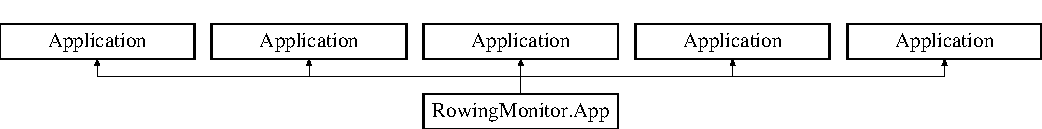
\includegraphics[height=1.709924cm]{class_rowing_monitor_1_1_app}
\end{center}
\end{figure}
\subsection*{Public Member Functions}
\begin{DoxyCompactItemize}
\item 
\hyperlink{class_rowing_monitor_1_1_app_a83d9e8a13163628ae72525843d35bbfe}{App} ()
\item 
void \hyperlink{class_rowing_monitor_1_1_app_a92cbce86d55626b5b411b795ec66c0c2}{Initialize\+Component} ()
\begin{DoxyCompactList}\small\item\em Initialize\+Component \end{DoxyCompactList}\item 
void \hyperlink{class_rowing_monitor_1_1_app_a92cbce86d55626b5b411b795ec66c0c2}{Initialize\+Component} ()
\begin{DoxyCompactList}\small\item\em Initialize\+Component \end{DoxyCompactList}\item 
void \hyperlink{class_rowing_monitor_1_1_app_a92cbce86d55626b5b411b795ec66c0c2}{Initialize\+Component} ()
\begin{DoxyCompactList}\small\item\em Initialize\+Component \end{DoxyCompactList}\item 
void \hyperlink{class_rowing_monitor_1_1_app_a92cbce86d55626b5b411b795ec66c0c2}{Initialize\+Component} ()
\begin{DoxyCompactList}\small\item\em Initialize\+Component \end{DoxyCompactList}\end{DoxyCompactItemize}
\subsection*{Static Public Member Functions}
\begin{DoxyCompactItemize}
\item 
static void \hyperlink{class_rowing_monitor_1_1_app_a3cb5b8569d044cd9687827e6c2072b7e}{Main} ()
\begin{DoxyCompactList}\small\item\em Application Entry Point. \end{DoxyCompactList}\item 
static void \hyperlink{class_rowing_monitor_1_1_app_a3cb5b8569d044cd9687827e6c2072b7e}{Main} ()
\begin{DoxyCompactList}\small\item\em Application Entry Point. \end{DoxyCompactList}\item 
static void \hyperlink{class_rowing_monitor_1_1_app_a3cb5b8569d044cd9687827e6c2072b7e}{Main} ()
\begin{DoxyCompactList}\small\item\em Application Entry Point. \end{DoxyCompactList}\item 
static void \hyperlink{class_rowing_monitor_1_1_app_a3cb5b8569d044cd9687827e6c2072b7e}{Main} ()
\begin{DoxyCompactList}\small\item\em Application Entry Point. \end{DoxyCompactList}\end{DoxyCompactItemize}
\subsection*{Protected Member Functions}
\begin{DoxyCompactItemize}
\item 
override void \hyperlink{class_rowing_monitor_1_1_app_a66e9b3baf5c2db1300758dddf3156f2f}{On\+Startup} (Startup\+Event\+Args e)
\end{DoxyCompactItemize}


\subsection{Detailed Description}
Interaktionslogik für \char`\"{}\+App.\+xaml\char`\"{} 

\hyperlink{class_rowing_monitor_1_1_app}{App} 

\subsection{Constructor \& Destructor Documentation}
\mbox{\Hypertarget{class_rowing_monitor_1_1_app_a83d9e8a13163628ae72525843d35bbfe}\label{class_rowing_monitor_1_1_app_a83d9e8a13163628ae72525843d35bbfe}} 
\index{Rowing\+Monitor\+::\+App@{Rowing\+Monitor\+::\+App}!App@{App}}
\index{App@{App}!Rowing\+Monitor\+::\+App@{Rowing\+Monitor\+::\+App}}
\subsubsection{\texorpdfstring{App()}{App()}}
{\footnotesize\ttfamily Rowing\+Monitor.\+App.\+App (\begin{DoxyParamCaption}{ }\end{DoxyParamCaption})}



\subsection{Member Function Documentation}
\mbox{\Hypertarget{class_rowing_monitor_1_1_app_a92cbce86d55626b5b411b795ec66c0c2}\label{class_rowing_monitor_1_1_app_a92cbce86d55626b5b411b795ec66c0c2}} 
\index{Rowing\+Monitor\+::\+App@{Rowing\+Monitor\+::\+App}!Initialize\+Component@{Initialize\+Component}}
\index{Initialize\+Component@{Initialize\+Component}!Rowing\+Monitor\+::\+App@{Rowing\+Monitor\+::\+App}}
\subsubsection{\texorpdfstring{Initialize\+Component()}{InitializeComponent()}\hspace{0.1cm}{\footnotesize\ttfamily [1/4]}}
{\footnotesize\ttfamily void Rowing\+Monitor.\+App.\+Initialize\+Component (\begin{DoxyParamCaption}{ }\end{DoxyParamCaption})}



Initialize\+Component 

\mbox{\Hypertarget{class_rowing_monitor_1_1_app_a92cbce86d55626b5b411b795ec66c0c2}\label{class_rowing_monitor_1_1_app_a92cbce86d55626b5b411b795ec66c0c2}} 
\index{Rowing\+Monitor\+::\+App@{Rowing\+Monitor\+::\+App}!Initialize\+Component@{Initialize\+Component}}
\index{Initialize\+Component@{Initialize\+Component}!Rowing\+Monitor\+::\+App@{Rowing\+Monitor\+::\+App}}
\subsubsection{\texorpdfstring{Initialize\+Component()}{InitializeComponent()}\hspace{0.1cm}{\footnotesize\ttfamily [2/4]}}
{\footnotesize\ttfamily void Rowing\+Monitor.\+App.\+Initialize\+Component (\begin{DoxyParamCaption}{ }\end{DoxyParamCaption})}



Initialize\+Component 

\mbox{\Hypertarget{class_rowing_monitor_1_1_app_a92cbce86d55626b5b411b795ec66c0c2}\label{class_rowing_monitor_1_1_app_a92cbce86d55626b5b411b795ec66c0c2}} 
\index{Rowing\+Monitor\+::\+App@{Rowing\+Monitor\+::\+App}!Initialize\+Component@{Initialize\+Component}}
\index{Initialize\+Component@{Initialize\+Component}!Rowing\+Monitor\+::\+App@{Rowing\+Monitor\+::\+App}}
\subsubsection{\texorpdfstring{Initialize\+Component()}{InitializeComponent()}\hspace{0.1cm}{\footnotesize\ttfamily [3/4]}}
{\footnotesize\ttfamily void Rowing\+Monitor.\+App.\+Initialize\+Component (\begin{DoxyParamCaption}{ }\end{DoxyParamCaption})}



Initialize\+Component 

\mbox{\Hypertarget{class_rowing_monitor_1_1_app_a92cbce86d55626b5b411b795ec66c0c2}\label{class_rowing_monitor_1_1_app_a92cbce86d55626b5b411b795ec66c0c2}} 
\index{Rowing\+Monitor\+::\+App@{Rowing\+Monitor\+::\+App}!Initialize\+Component@{Initialize\+Component}}
\index{Initialize\+Component@{Initialize\+Component}!Rowing\+Monitor\+::\+App@{Rowing\+Monitor\+::\+App}}
\subsubsection{\texorpdfstring{Initialize\+Component()}{InitializeComponent()}\hspace{0.1cm}{\footnotesize\ttfamily [4/4]}}
{\footnotesize\ttfamily void Rowing\+Monitor.\+App.\+Initialize\+Component (\begin{DoxyParamCaption}{ }\end{DoxyParamCaption})}



Initialize\+Component 

\mbox{\Hypertarget{class_rowing_monitor_1_1_app_a3cb5b8569d044cd9687827e6c2072b7e}\label{class_rowing_monitor_1_1_app_a3cb5b8569d044cd9687827e6c2072b7e}} 
\index{Rowing\+Monitor\+::\+App@{Rowing\+Monitor\+::\+App}!Main@{Main}}
\index{Main@{Main}!Rowing\+Monitor\+::\+App@{Rowing\+Monitor\+::\+App}}
\subsubsection{\texorpdfstring{Main()}{Main()}\hspace{0.1cm}{\footnotesize\ttfamily [1/4]}}
{\footnotesize\ttfamily static void Rowing\+Monitor.\+App.\+Main (\begin{DoxyParamCaption}{ }\end{DoxyParamCaption})\hspace{0.3cm}{\ttfamily [static]}}



Application Entry Point. 

\mbox{\Hypertarget{class_rowing_monitor_1_1_app_a3cb5b8569d044cd9687827e6c2072b7e}\label{class_rowing_monitor_1_1_app_a3cb5b8569d044cd9687827e6c2072b7e}} 
\index{Rowing\+Monitor\+::\+App@{Rowing\+Monitor\+::\+App}!Main@{Main}}
\index{Main@{Main}!Rowing\+Monitor\+::\+App@{Rowing\+Monitor\+::\+App}}
\subsubsection{\texorpdfstring{Main()}{Main()}\hspace{0.1cm}{\footnotesize\ttfamily [2/4]}}
{\footnotesize\ttfamily static void Rowing\+Monitor.\+App.\+Main (\begin{DoxyParamCaption}{ }\end{DoxyParamCaption})\hspace{0.3cm}{\ttfamily [static]}}



Application Entry Point. 

\mbox{\Hypertarget{class_rowing_monitor_1_1_app_a3cb5b8569d044cd9687827e6c2072b7e}\label{class_rowing_monitor_1_1_app_a3cb5b8569d044cd9687827e6c2072b7e}} 
\index{Rowing\+Monitor\+::\+App@{Rowing\+Monitor\+::\+App}!Main@{Main}}
\index{Main@{Main}!Rowing\+Monitor\+::\+App@{Rowing\+Monitor\+::\+App}}
\subsubsection{\texorpdfstring{Main()}{Main()}\hspace{0.1cm}{\footnotesize\ttfamily [3/4]}}
{\footnotesize\ttfamily static void Rowing\+Monitor.\+App.\+Main (\begin{DoxyParamCaption}{ }\end{DoxyParamCaption})\hspace{0.3cm}{\ttfamily [static]}}



Application Entry Point. 

\mbox{\Hypertarget{class_rowing_monitor_1_1_app_a3cb5b8569d044cd9687827e6c2072b7e}\label{class_rowing_monitor_1_1_app_a3cb5b8569d044cd9687827e6c2072b7e}} 
\index{Rowing\+Monitor\+::\+App@{Rowing\+Monitor\+::\+App}!Main@{Main}}
\index{Main@{Main}!Rowing\+Monitor\+::\+App@{Rowing\+Monitor\+::\+App}}
\subsubsection{\texorpdfstring{Main()}{Main()}\hspace{0.1cm}{\footnotesize\ttfamily [4/4]}}
{\footnotesize\ttfamily static void Rowing\+Monitor.\+App.\+Main (\begin{DoxyParamCaption}{ }\end{DoxyParamCaption})\hspace{0.3cm}{\ttfamily [static]}}



Application Entry Point. 

\mbox{\Hypertarget{class_rowing_monitor_1_1_app_a66e9b3baf5c2db1300758dddf3156f2f}\label{class_rowing_monitor_1_1_app_a66e9b3baf5c2db1300758dddf3156f2f}} 
\index{Rowing\+Monitor\+::\+App@{Rowing\+Monitor\+::\+App}!On\+Startup@{On\+Startup}}
\index{On\+Startup@{On\+Startup}!Rowing\+Monitor\+::\+App@{Rowing\+Monitor\+::\+App}}
\subsubsection{\texorpdfstring{On\+Startup()}{OnStartup()}}
{\footnotesize\ttfamily override void Rowing\+Monitor.\+App.\+On\+Startup (\begin{DoxyParamCaption}\item[{Startup\+Event\+Args}]{e }\end{DoxyParamCaption})\hspace{0.3cm}{\ttfamily [protected]}}



The documentation for this class was generated from the following files\+:\begin{DoxyCompactItemize}
\item 
\hyperlink{_app_8xaml_8cs}{App.\+xaml.\+cs}\item 
obj/\+Debug/\hyperlink{_debug_2_app_8g_8cs}{App.\+g.\+cs}\item 
obj/\+Debug/\hyperlink{_debug_2_app_8g_8i_8cs}{App.\+g.\+i.\+cs}\end{DoxyCompactItemize}

\hypertarget{class_rowing_monitor_1_1_model_1_1_body_not_fully_tracked_exception}{}\section{Rowing\+Monitor.\+Model.\+Body\+Not\+Fully\+Tracked\+Exception Class Reference}
\label{class_rowing_monitor_1_1_model_1_1_body_not_fully_tracked_exception}\index{Rowing\+Monitor.\+Model.\+Body\+Not\+Fully\+Tracked\+Exception@{Rowing\+Monitor.\+Model.\+Body\+Not\+Fully\+Tracked\+Exception}}
Inheritance diagram for Rowing\+Monitor.\+Model.\+Body\+Not\+Fully\+Tracked\+Exception\+:\begin{figure}[H]
\begin{center}
\leavevmode
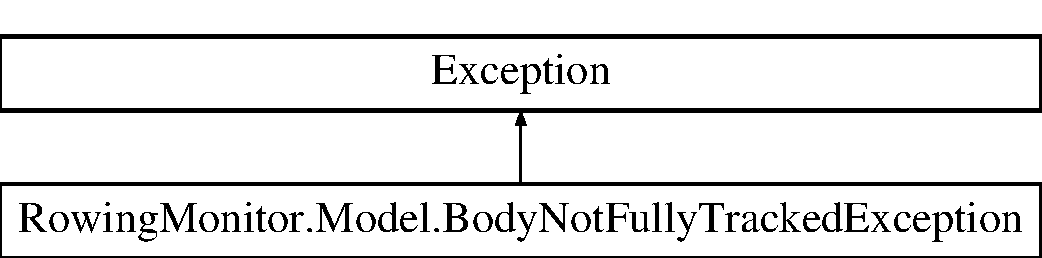
\includegraphics[height=2.000000cm]{class_rowing_monitor_1_1_model_1_1_body_not_fully_tracked_exception}
\end{center}
\end{figure}


The documentation for this class was generated from the following file\+:\begin{DoxyCompactItemize}
\item 
Model/\+Util/\hyperlink{_body_not_fully_tracked_exception_8cs}{Body\+Not\+Fully\+Tracked\+Exception.\+cs}\end{DoxyCompactItemize}

\hypertarget{class_rowing_monitor_1_1_model_1_1_calculated_frame_arrived_event_args}{}\section{Rowing\+Monitor.\+Model.\+Calculated\+Frame\+Arrived\+Event\+Args Class Reference}
\label{class_rowing_monitor_1_1_model_1_1_calculated_frame_arrived_event_args}\index{Rowing\+Monitor.\+Model.\+Calculated\+Frame\+Arrived\+Event\+Args@{Rowing\+Monitor.\+Model.\+Calculated\+Frame\+Arrived\+Event\+Args}}


Represents the arguments for a calculated frame arrived event.  


Inheritance diagram for Rowing\+Monitor.\+Model.\+Calculated\+Frame\+Arrived\+Event\+Args\+:\begin{figure}[H]
\begin{center}
\leavevmode
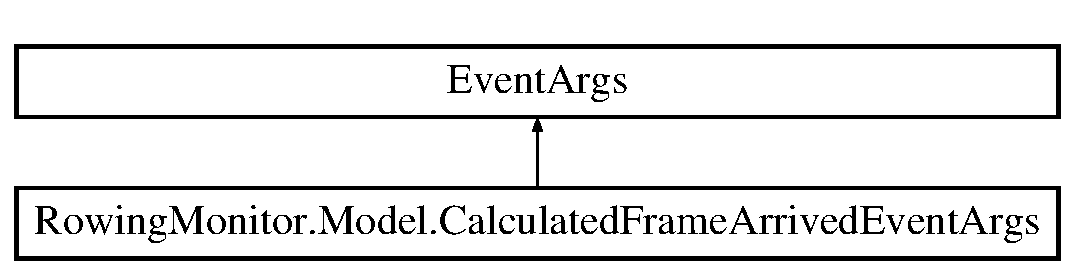
\includegraphics[height=2.000000cm]{class_rowing_monitor_1_1_model_1_1_calculated_frame_arrived_event_args}
\end{center}
\end{figure}
\subsection*{Public Member Functions}
\begin{DoxyCompactItemize}
\item 
\hyperlink{class_rowing_monitor_1_1_model_1_1_calculated_frame_arrived_event_args_ab73cb44f37b699c76ed2a5b1d98338d3}{Calculated\+Frame\+Arrived\+Event\+Args} (\hyperlink{struct_rowing_monitor_1_1_model_1_1_util_1_1_joint_data}{Joint\+Data} calculated\+Joint\+Data)
\end{DoxyCompactItemize}
\subsection*{Properties}
\begin{DoxyCompactItemize}
\item 
\hyperlink{struct_rowing_monitor_1_1_model_1_1_util_1_1_joint_data}{Joint\+Data} \hyperlink{class_rowing_monitor_1_1_model_1_1_calculated_frame_arrived_event_args_ad2a6d96247f32cec46b5e5006b4a867b}{Calculated\+Joint\+Data}\hspace{0.3cm}{\ttfamily  \mbox{[}get\mbox{]}}
\end{DoxyCompactItemize}


\subsection{Detailed Description}
Represents the arguments for a calculated frame arrived event. 



\subsection{Constructor \& Destructor Documentation}
\mbox{\Hypertarget{class_rowing_monitor_1_1_model_1_1_calculated_frame_arrived_event_args_ab73cb44f37b699c76ed2a5b1d98338d3}\label{class_rowing_monitor_1_1_model_1_1_calculated_frame_arrived_event_args_ab73cb44f37b699c76ed2a5b1d98338d3}} 
\index{Rowing\+Monitor\+::\+Model\+::\+Calculated\+Frame\+Arrived\+Event\+Args@{Rowing\+Monitor\+::\+Model\+::\+Calculated\+Frame\+Arrived\+Event\+Args}!Calculated\+Frame\+Arrived\+Event\+Args@{Calculated\+Frame\+Arrived\+Event\+Args}}
\index{Calculated\+Frame\+Arrived\+Event\+Args@{Calculated\+Frame\+Arrived\+Event\+Args}!Rowing\+Monitor\+::\+Model\+::\+Calculated\+Frame\+Arrived\+Event\+Args@{Rowing\+Monitor\+::\+Model\+::\+Calculated\+Frame\+Arrived\+Event\+Args}}
\subsubsection{\texorpdfstring{Calculated\+Frame\+Arrived\+Event\+Args()}{CalculatedFrameArrivedEventArgs()}}
{\footnotesize\ttfamily Rowing\+Monitor.\+Model.\+Calculated\+Frame\+Arrived\+Event\+Args.\+Calculated\+Frame\+Arrived\+Event\+Args (\begin{DoxyParamCaption}\item[{\hyperlink{struct_rowing_monitor_1_1_model_1_1_util_1_1_joint_data}{Joint\+Data}}]{calculated\+Joint\+Data }\end{DoxyParamCaption})}



\subsection{Property Documentation}
\mbox{\Hypertarget{class_rowing_monitor_1_1_model_1_1_calculated_frame_arrived_event_args_ad2a6d96247f32cec46b5e5006b4a867b}\label{class_rowing_monitor_1_1_model_1_1_calculated_frame_arrived_event_args_ad2a6d96247f32cec46b5e5006b4a867b}} 
\index{Rowing\+Monitor\+::\+Model\+::\+Calculated\+Frame\+Arrived\+Event\+Args@{Rowing\+Monitor\+::\+Model\+::\+Calculated\+Frame\+Arrived\+Event\+Args}!Calculated\+Joint\+Data@{Calculated\+Joint\+Data}}
\index{Calculated\+Joint\+Data@{Calculated\+Joint\+Data}!Rowing\+Monitor\+::\+Model\+::\+Calculated\+Frame\+Arrived\+Event\+Args@{Rowing\+Monitor\+::\+Model\+::\+Calculated\+Frame\+Arrived\+Event\+Args}}
\subsubsection{\texorpdfstring{Calculated\+Joint\+Data}{CalculatedJointData}}
{\footnotesize\ttfamily \hyperlink{struct_rowing_monitor_1_1_model_1_1_util_1_1_joint_data}{Joint\+Data} Rowing\+Monitor.\+Model.\+Calculated\+Frame\+Arrived\+Event\+Args.\+Calculated\+Joint\+Data\hspace{0.3cm}{\ttfamily [get]}}



The documentation for this class was generated from the following file\+:\begin{DoxyCompactItemize}
\item 
Model/\+Event\+Args/\hyperlink{_calculated_frame_arrived_event_args_8cs}{Calculated\+Frame\+Arrived\+Event\+Args.\+cs}\end{DoxyCompactItemize}

\hypertarget{class_rowing_monitor_1_1_model_1_1_util_1_1_circular_buffer}{}\section{Rowing\+Monitor.\+Model.\+Util.\+Circular\+Buffer Class Reference}
\label{class_rowing_monitor_1_1_model_1_1_util_1_1_circular_buffer}\index{Rowing\+Monitor.\+Model.\+Util.\+Circular\+Buffer@{Rowing\+Monitor.\+Model.\+Util.\+Circular\+Buffer}}


A F\+I\+FO buffer which overwrites old values if the size is reached.  


\subsection*{Public Member Functions}
\begin{DoxyCompactItemize}
\item 
\hyperlink{class_rowing_monitor_1_1_model_1_1_util_1_1_circular_buffer_a733322a69fc230d62c34e7704c0b63b1}{Circular\+Buffer} (int size)
\item 
void \hyperlink{class_rowing_monitor_1_1_model_1_1_util_1_1_circular_buffer_af301723b675ac785291d5d234c5557c7}{Enqueue} (object obj)
\item 
object \mbox{[}$\,$\mbox{]} \hyperlink{class_rowing_monitor_1_1_model_1_1_util_1_1_circular_buffer_a63e22497a191f7a4352e5aed13ce7e4a}{To\+Array} ()
\end{DoxyCompactItemize}


\subsection{Detailed Description}
A F\+I\+FO buffer which overwrites old values if the size is reached. 



\subsection{Constructor \& Destructor Documentation}
\mbox{\Hypertarget{class_rowing_monitor_1_1_model_1_1_util_1_1_circular_buffer_a733322a69fc230d62c34e7704c0b63b1}\label{class_rowing_monitor_1_1_model_1_1_util_1_1_circular_buffer_a733322a69fc230d62c34e7704c0b63b1}} 
\index{Rowing\+Monitor\+::\+Model\+::\+Util\+::\+Circular\+Buffer@{Rowing\+Monitor\+::\+Model\+::\+Util\+::\+Circular\+Buffer}!Circular\+Buffer@{Circular\+Buffer}}
\index{Circular\+Buffer@{Circular\+Buffer}!Rowing\+Monitor\+::\+Model\+::\+Util\+::\+Circular\+Buffer@{Rowing\+Monitor\+::\+Model\+::\+Util\+::\+Circular\+Buffer}}
\subsubsection{\texorpdfstring{Circular\+Buffer()}{CircularBuffer()}}
{\footnotesize\ttfamily Rowing\+Monitor.\+Model.\+Util.\+Circular\+Buffer.\+Circular\+Buffer (\begin{DoxyParamCaption}\item[{int}]{size }\end{DoxyParamCaption})}



\subsection{Member Function Documentation}
\mbox{\Hypertarget{class_rowing_monitor_1_1_model_1_1_util_1_1_circular_buffer_af301723b675ac785291d5d234c5557c7}\label{class_rowing_monitor_1_1_model_1_1_util_1_1_circular_buffer_af301723b675ac785291d5d234c5557c7}} 
\index{Rowing\+Monitor\+::\+Model\+::\+Util\+::\+Circular\+Buffer@{Rowing\+Monitor\+::\+Model\+::\+Util\+::\+Circular\+Buffer}!Enqueue@{Enqueue}}
\index{Enqueue@{Enqueue}!Rowing\+Monitor\+::\+Model\+::\+Util\+::\+Circular\+Buffer@{Rowing\+Monitor\+::\+Model\+::\+Util\+::\+Circular\+Buffer}}
\subsubsection{\texorpdfstring{Enqueue()}{Enqueue()}}
{\footnotesize\ttfamily void Rowing\+Monitor.\+Model.\+Util.\+Circular\+Buffer.\+Enqueue (\begin{DoxyParamCaption}\item[{object}]{obj }\end{DoxyParamCaption})}

\mbox{\Hypertarget{class_rowing_monitor_1_1_model_1_1_util_1_1_circular_buffer_a63e22497a191f7a4352e5aed13ce7e4a}\label{class_rowing_monitor_1_1_model_1_1_util_1_1_circular_buffer_a63e22497a191f7a4352e5aed13ce7e4a}} 
\index{Rowing\+Monitor\+::\+Model\+::\+Util\+::\+Circular\+Buffer@{Rowing\+Monitor\+::\+Model\+::\+Util\+::\+Circular\+Buffer}!To\+Array@{To\+Array}}
\index{To\+Array@{To\+Array}!Rowing\+Monitor\+::\+Model\+::\+Util\+::\+Circular\+Buffer@{Rowing\+Monitor\+::\+Model\+::\+Util\+::\+Circular\+Buffer}}
\subsubsection{\texorpdfstring{To\+Array()}{ToArray()}}
{\footnotesize\ttfamily object \mbox{[}$\,$\mbox{]} Rowing\+Monitor.\+Model.\+Util.\+Circular\+Buffer.\+To\+Array (\begin{DoxyParamCaption}{ }\end{DoxyParamCaption})}



The documentation for this class was generated from the following file\+:\begin{DoxyCompactItemize}
\item 
Model/\+Util/\hyperlink{_circular_buffer_8cs}{Circular\+Buffer.\+cs}\end{DoxyCompactItemize}

\hypertarget{class_rowing_monitor_1_1_view_1_1_coach_view}{}\section{Rowing\+Monitor.\+View.\+Coach\+View Class Reference}
\label{class_rowing_monitor_1_1_view_1_1_coach_view}\index{Rowing\+Monitor.\+View.\+Coach\+View@{Rowing\+Monitor.\+View.\+Coach\+View}}


\hyperlink{class_rowing_monitor_1_1_view_1_1_coach_view}{Coach\+View}  


Inheritance diagram for Rowing\+Monitor.\+View.\+Coach\+View\+:\begin{figure}[H]
\begin{center}
\leavevmode
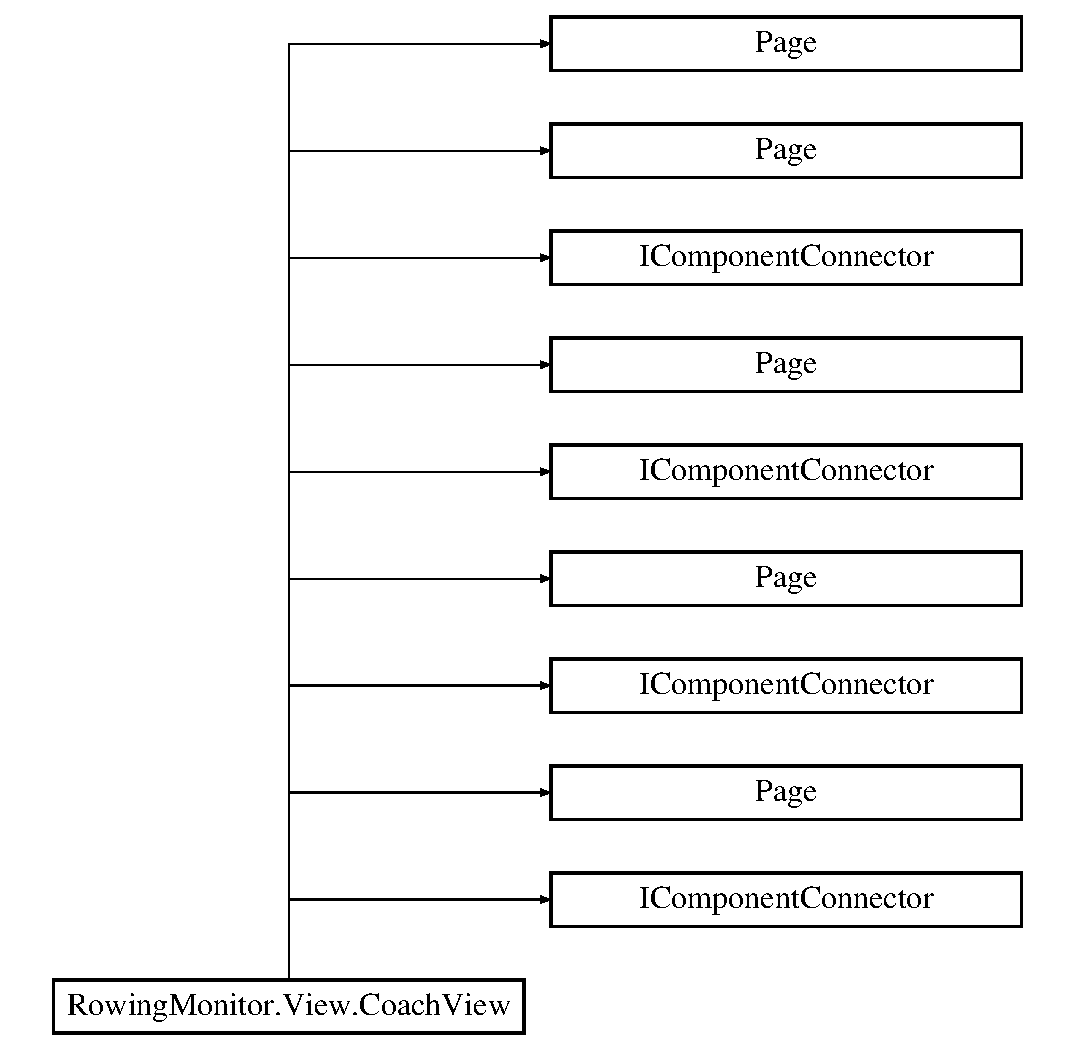
\includegraphics[height=10.000000cm]{class_rowing_monitor_1_1_view_1_1_coach_view}
\end{center}
\end{figure}
\subsection*{Public Member Functions}
\begin{DoxyCompactItemize}
\item 
void \hyperlink{class_rowing_monitor_1_1_view_1_1_coach_view_a4751c9ab7f066dceb54766893a536101}{Initialize\+Component} ()
\begin{DoxyCompactList}\small\item\em Initialize\+Component \end{DoxyCompactList}\item 
void \hyperlink{class_rowing_monitor_1_1_view_1_1_coach_view_a4751c9ab7f066dceb54766893a536101}{Initialize\+Component} ()
\begin{DoxyCompactList}\small\item\em Initialize\+Component \end{DoxyCompactList}\item 
void \hyperlink{class_rowing_monitor_1_1_view_1_1_coach_view_a4751c9ab7f066dceb54766893a536101}{Initialize\+Component} ()
\begin{DoxyCompactList}\small\item\em Initialize\+Component \end{DoxyCompactList}\item 
void \hyperlink{class_rowing_monitor_1_1_view_1_1_coach_view_a4751c9ab7f066dceb54766893a536101}{Initialize\+Component} ()
\begin{DoxyCompactList}\small\item\em Initialize\+Component \end{DoxyCompactList}\item 
\hyperlink{class_rowing_monitor_1_1_view_1_1_coach_view_acc1611840e2208b5dacd8bdd1927fef0}{Coach\+View} ()
\end{DoxyCompactItemize}


\subsection{Detailed Description}
\hyperlink{class_rowing_monitor_1_1_view_1_1_coach_view}{Coach\+View} 

Interaktionslogik für Coach\+View.\+xaml 

\subsection{Constructor \& Destructor Documentation}
\mbox{\Hypertarget{class_rowing_monitor_1_1_view_1_1_coach_view_acc1611840e2208b5dacd8bdd1927fef0}\label{class_rowing_monitor_1_1_view_1_1_coach_view_acc1611840e2208b5dacd8bdd1927fef0}} 
\index{Rowing\+Monitor\+::\+View\+::\+Coach\+View@{Rowing\+Monitor\+::\+View\+::\+Coach\+View}!Coach\+View@{Coach\+View}}
\index{Coach\+View@{Coach\+View}!Rowing\+Monitor\+::\+View\+::\+Coach\+View@{Rowing\+Monitor\+::\+View\+::\+Coach\+View}}
\subsubsection{\texorpdfstring{Coach\+View()}{CoachView()}}
{\footnotesize\ttfamily Rowing\+Monitor.\+View.\+Coach\+View.\+Coach\+View (\begin{DoxyParamCaption}{ }\end{DoxyParamCaption})}



\subsection{Member Function Documentation}
\mbox{\Hypertarget{class_rowing_monitor_1_1_view_1_1_coach_view_a4751c9ab7f066dceb54766893a536101}\label{class_rowing_monitor_1_1_view_1_1_coach_view_a4751c9ab7f066dceb54766893a536101}} 
\index{Rowing\+Monitor\+::\+View\+::\+Coach\+View@{Rowing\+Monitor\+::\+View\+::\+Coach\+View}!Initialize\+Component@{Initialize\+Component}}
\index{Initialize\+Component@{Initialize\+Component}!Rowing\+Monitor\+::\+View\+::\+Coach\+View@{Rowing\+Monitor\+::\+View\+::\+Coach\+View}}
\subsubsection{\texorpdfstring{Initialize\+Component()}{InitializeComponent()}\hspace{0.1cm}{\footnotesize\ttfamily [1/4]}}
{\footnotesize\ttfamily void Rowing\+Monitor.\+View.\+Coach\+View.\+Initialize\+Component (\begin{DoxyParamCaption}{ }\end{DoxyParamCaption})}



Initialize\+Component 

\mbox{\Hypertarget{class_rowing_monitor_1_1_view_1_1_coach_view_a4751c9ab7f066dceb54766893a536101}\label{class_rowing_monitor_1_1_view_1_1_coach_view_a4751c9ab7f066dceb54766893a536101}} 
\index{Rowing\+Monitor\+::\+View\+::\+Coach\+View@{Rowing\+Monitor\+::\+View\+::\+Coach\+View}!Initialize\+Component@{Initialize\+Component}}
\index{Initialize\+Component@{Initialize\+Component}!Rowing\+Monitor\+::\+View\+::\+Coach\+View@{Rowing\+Monitor\+::\+View\+::\+Coach\+View}}
\subsubsection{\texorpdfstring{Initialize\+Component()}{InitializeComponent()}\hspace{0.1cm}{\footnotesize\ttfamily [2/4]}}
{\footnotesize\ttfamily void Rowing\+Monitor.\+View.\+Coach\+View.\+Initialize\+Component (\begin{DoxyParamCaption}{ }\end{DoxyParamCaption})}



Initialize\+Component 

\mbox{\Hypertarget{class_rowing_monitor_1_1_view_1_1_coach_view_a4751c9ab7f066dceb54766893a536101}\label{class_rowing_monitor_1_1_view_1_1_coach_view_a4751c9ab7f066dceb54766893a536101}} 
\index{Rowing\+Monitor\+::\+View\+::\+Coach\+View@{Rowing\+Monitor\+::\+View\+::\+Coach\+View}!Initialize\+Component@{Initialize\+Component}}
\index{Initialize\+Component@{Initialize\+Component}!Rowing\+Monitor\+::\+View\+::\+Coach\+View@{Rowing\+Monitor\+::\+View\+::\+Coach\+View}}
\subsubsection{\texorpdfstring{Initialize\+Component()}{InitializeComponent()}\hspace{0.1cm}{\footnotesize\ttfamily [3/4]}}
{\footnotesize\ttfamily void Rowing\+Monitor.\+View.\+Coach\+View.\+Initialize\+Component (\begin{DoxyParamCaption}{ }\end{DoxyParamCaption})}



Initialize\+Component 

\mbox{\Hypertarget{class_rowing_monitor_1_1_view_1_1_coach_view_a4751c9ab7f066dceb54766893a536101}\label{class_rowing_monitor_1_1_view_1_1_coach_view_a4751c9ab7f066dceb54766893a536101}} 
\index{Rowing\+Monitor\+::\+View\+::\+Coach\+View@{Rowing\+Monitor\+::\+View\+::\+Coach\+View}!Initialize\+Component@{Initialize\+Component}}
\index{Initialize\+Component@{Initialize\+Component}!Rowing\+Monitor\+::\+View\+::\+Coach\+View@{Rowing\+Monitor\+::\+View\+::\+Coach\+View}}
\subsubsection{\texorpdfstring{Initialize\+Component()}{InitializeComponent()}\hspace{0.1cm}{\footnotesize\ttfamily [4/4]}}
{\footnotesize\ttfamily void Rowing\+Monitor.\+View.\+Coach\+View.\+Initialize\+Component (\begin{DoxyParamCaption}{ }\end{DoxyParamCaption})}



Initialize\+Component 



The documentation for this class was generated from the following files\+:\begin{DoxyCompactItemize}
\item 
obj/\+Debug/\+View/\hyperlink{_debug_2_view_2_coach_view_8g_8cs}{Coach\+View.\+g.\+cs}\item 
obj/\+Debug/\+View/\hyperlink{_debug_2_view_2_coach_view_8g_8i_8cs}{Coach\+View.\+g.\+i.\+cs}\item 
View/\hyperlink{_coach_view_8xaml_8cs}{Coach\+View.\+xaml.\+cs}\end{DoxyCompactItemize}

\hypertarget{class_rowing_monitor_1_1_view_model_1_1_coach_view_model}{}\section{Rowing\+Monitor.\+View\+Model.\+Coach\+View\+Model Class Reference}
\label{class_rowing_monitor_1_1_view_model_1_1_coach_view_model}\index{Rowing\+Monitor.\+View\+Model.\+Coach\+View\+Model@{Rowing\+Monitor.\+View\+Model.\+Coach\+View\+Model}}
Inheritance diagram for Rowing\+Monitor.\+View\+Model.\+Coach\+View\+Model\+:\begin{figure}[H]
\begin{center}
\leavevmode
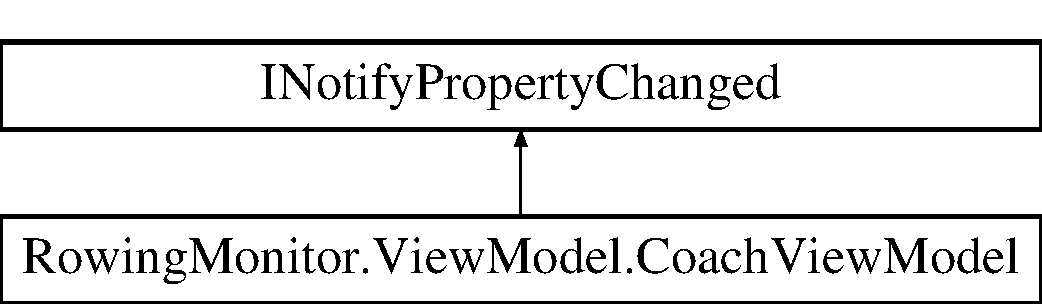
\includegraphics[height=2.000000cm]{class_rowing_monitor_1_1_view_model_1_1_coach_view_model}
\end{center}
\end{figure}
\subsection*{Public Member Functions}
\begin{DoxyCompactItemize}
\item 
\hyperlink{class_rowing_monitor_1_1_view_model_1_1_coach_view_model_a083e3b3fd6d99f73f46dfffd5a65f40a}{Coach\+View\+Model} ()
\item 
void \hyperlink{class_rowing_monitor_1_1_view_model_1_1_coach_view_model_aae36b0bb86b83b32b3cfe576fd917e7f}{View\+Loaded} ()
\item 
void \hyperlink{class_rowing_monitor_1_1_view_model_1_1_coach_view_model_a65df739b4a9b22d3241cf7afd18c0256}{View\+Unloaded} ()
\end{DoxyCompactItemize}
\subsection*{Properties}
\begin{DoxyCompactItemize}
\item 
Grid \hyperlink{class_rowing_monitor_1_1_view_model_1_1_coach_view_model_a7f736b8421cccf54c5b2c745c06c5e03}{Main\+Grid}\hspace{0.3cm}{\ttfamily  \mbox{[}get, set\mbox{]}}
\item 
string \hyperlink{class_rowing_monitor_1_1_view_model_1_1_coach_view_model_a698a6cf6a217844cef7c4173d36b8c31}{Session\+Time}\hspace{0.3cm}{\ttfamily  \mbox{[}get, set\mbox{]}}
\item 
string \hyperlink{class_rowing_monitor_1_1_view_model_1_1_coach_view_model_a9040dc6478b7f4f262d6be12642d7336}{Stroke\+Count}\hspace{0.3cm}{\ttfamily  \mbox{[}get, set\mbox{]}}
\item 
string \hyperlink{class_rowing_monitor_1_1_view_model_1_1_coach_view_model_a3b58669348fd3255eafae893d187e096}{Stroke\+Rate}\hspace{0.3cm}{\ttfamily  \mbox{[}get, set\mbox{]}}
\item 
string \hyperlink{class_rowing_monitor_1_1_view_model_1_1_coach_view_model_acca7bb0eeaae1c4b6f7ae6d06c0aa772}{Stroke\+Length}\hspace{0.3cm}{\ttfamily  \mbox{[}get, set\mbox{]}}
\item 
string \hyperlink{class_rowing_monitor_1_1_view_model_1_1_coach_view_model_aba749823320c686335dc09514bc8b6ab}{Mean\+Stroke\+Length}\hspace{0.3cm}{\ttfamily  \mbox{[}get, set\mbox{]}}
\item 
string \hyperlink{class_rowing_monitor_1_1_view_model_1_1_coach_view_model_a58d4825060e0b59a33fadb20883704eb}{Seat\+Travel}\hspace{0.3cm}{\ttfamily  \mbox{[}get, set\mbox{]}}
\item 
string \hyperlink{class_rowing_monitor_1_1_view_model_1_1_coach_view_model_a6a7e565b8183152d1894b9ca31184371}{Mean\+Seat\+Travel}\hspace{0.3cm}{\ttfamily  \mbox{[}get, set\mbox{]}}
\item 
string \hyperlink{class_rowing_monitor_1_1_view_model_1_1_coach_view_model_ab2037da08e713466849266a8a0bce535}{Stroke\+Time}\hspace{0.3cm}{\ttfamily  \mbox{[}get, set\mbox{]}}
\item 
string \hyperlink{class_rowing_monitor_1_1_view_model_1_1_coach_view_model_a4524d8e7f6e93686d46e26df699c956d}{Mean\+Stroke\+Time}\hspace{0.3cm}{\ttfamily  \mbox{[}get, set\mbox{]}}
\item 
string \hyperlink{class_rowing_monitor_1_1_view_model_1_1_coach_view_model_a61256f169d1e75c1f3d8fa7805d5e757}{Max\+Handle\+Velocity}\hspace{0.3cm}{\ttfamily  \mbox{[}get, set\mbox{]}}
\item 
string \hyperlink{class_rowing_monitor_1_1_view_model_1_1_coach_view_model_aba6a7eb887398580daaf9567bcf36d3f}{Mean\+Max\+Handle\+Velocity}\hspace{0.3cm}{\ttfamily  \mbox{[}get, set\mbox{]}}
\item 
string \hyperlink{class_rowing_monitor_1_1_view_model_1_1_coach_view_model_a438fdc5df5ae18d8cd154504912d9b65}{Max\+Legs\+Velocity}\hspace{0.3cm}{\ttfamily  \mbox{[}get, set\mbox{]}}
\item 
string \hyperlink{class_rowing_monitor_1_1_view_model_1_1_coach_view_model_aeac341cb4dc82ce1a7e784fdb7aa2aa9}{Mean\+Max\+Legs\+Velocity}\hspace{0.3cm}{\ttfamily  \mbox{[}get, set\mbox{]}}
\item 
string \hyperlink{class_rowing_monitor_1_1_view_model_1_1_coach_view_model_a8c119b77046f9ebc29a8bc51253423a1}{Max\+Arms\+Velocity}\hspace{0.3cm}{\ttfamily  \mbox{[}get, set\mbox{]}}
\item 
string \hyperlink{class_rowing_monitor_1_1_view_model_1_1_coach_view_model_ade526b71315b0698a4d784f0e4bc2860}{Mean\+Max\+Arms\+Velocity}\hspace{0.3cm}{\ttfamily  \mbox{[}get, set\mbox{]}}
\item 
string \hyperlink{class_rowing_monitor_1_1_view_model_1_1_coach_view_model_adc7d37e55dc2ac669f81356f9a2bc079}{Max\+Trunk\+Velocity}\hspace{0.3cm}{\ttfamily  \mbox{[}get, set\mbox{]}}
\item 
string \hyperlink{class_rowing_monitor_1_1_view_model_1_1_coach_view_model_a913a7dd526cef93b33d4d7a6dd85209c}{Mean\+Max\+Trunk\+Velocity}\hspace{0.3cm}{\ttfamily  \mbox{[}get, set\mbox{]}}
\item 
string \hyperlink{class_rowing_monitor_1_1_view_model_1_1_coach_view_model_a72b074890be114e880646d6856e1038d}{Mean\+Catch\+Factor}\hspace{0.3cm}{\ttfamily  \mbox{[}get, set\mbox{]}}
\item 
string \hyperlink{class_rowing_monitor_1_1_view_model_1_1_coach_view_model_a4d6e272b54fefc1195b28e6cadaa4b34}{Mean\+Rowing\+Style\+Factor}\hspace{0.3cm}{\ttfamily  \mbox{[}get, set\mbox{]}}
\end{DoxyCompactItemize}
\subsection*{Events}
\begin{DoxyCompactItemize}
\item 
Property\+Changed\+Event\+Handler \hyperlink{class_rowing_monitor_1_1_view_model_1_1_coach_view_model_ab3364d1cd88e9e02b866ae2a7f3fe688}{Property\+Changed}
\end{DoxyCompactItemize}


\subsection{Constructor \& Destructor Documentation}
\mbox{\Hypertarget{class_rowing_monitor_1_1_view_model_1_1_coach_view_model_a083e3b3fd6d99f73f46dfffd5a65f40a}\label{class_rowing_monitor_1_1_view_model_1_1_coach_view_model_a083e3b3fd6d99f73f46dfffd5a65f40a}} 
\index{Rowing\+Monitor\+::\+View\+Model\+::\+Coach\+View\+Model@{Rowing\+Monitor\+::\+View\+Model\+::\+Coach\+View\+Model}!Coach\+View\+Model@{Coach\+View\+Model}}
\index{Coach\+View\+Model@{Coach\+View\+Model}!Rowing\+Monitor\+::\+View\+Model\+::\+Coach\+View\+Model@{Rowing\+Monitor\+::\+View\+Model\+::\+Coach\+View\+Model}}
\subsubsection{\texorpdfstring{Coach\+View\+Model()}{CoachViewModel()}}
{\footnotesize\ttfamily Rowing\+Monitor.\+View\+Model.\+Coach\+View\+Model.\+Coach\+View\+Model (\begin{DoxyParamCaption}{ }\end{DoxyParamCaption})}



\subsection{Member Function Documentation}
\mbox{\Hypertarget{class_rowing_monitor_1_1_view_model_1_1_coach_view_model_aae36b0bb86b83b32b3cfe576fd917e7f}\label{class_rowing_monitor_1_1_view_model_1_1_coach_view_model_aae36b0bb86b83b32b3cfe576fd917e7f}} 
\index{Rowing\+Monitor\+::\+View\+Model\+::\+Coach\+View\+Model@{Rowing\+Monitor\+::\+View\+Model\+::\+Coach\+View\+Model}!View\+Loaded@{View\+Loaded}}
\index{View\+Loaded@{View\+Loaded}!Rowing\+Monitor\+::\+View\+Model\+::\+Coach\+View\+Model@{Rowing\+Monitor\+::\+View\+Model\+::\+Coach\+View\+Model}}
\subsubsection{\texorpdfstring{View\+Loaded()}{ViewLoaded()}}
{\footnotesize\ttfamily void Rowing\+Monitor.\+View\+Model.\+Coach\+View\+Model.\+View\+Loaded (\begin{DoxyParamCaption}{ }\end{DoxyParamCaption})}

\mbox{\Hypertarget{class_rowing_monitor_1_1_view_model_1_1_coach_view_model_a65df739b4a9b22d3241cf7afd18c0256}\label{class_rowing_monitor_1_1_view_model_1_1_coach_view_model_a65df739b4a9b22d3241cf7afd18c0256}} 
\index{Rowing\+Monitor\+::\+View\+Model\+::\+Coach\+View\+Model@{Rowing\+Monitor\+::\+View\+Model\+::\+Coach\+View\+Model}!View\+Unloaded@{View\+Unloaded}}
\index{View\+Unloaded@{View\+Unloaded}!Rowing\+Monitor\+::\+View\+Model\+::\+Coach\+View\+Model@{Rowing\+Monitor\+::\+View\+Model\+::\+Coach\+View\+Model}}
\subsubsection{\texorpdfstring{View\+Unloaded()}{ViewUnloaded()}}
{\footnotesize\ttfamily void Rowing\+Monitor.\+View\+Model.\+Coach\+View\+Model.\+View\+Unloaded (\begin{DoxyParamCaption}{ }\end{DoxyParamCaption})}



\subsection{Property Documentation}
\mbox{\Hypertarget{class_rowing_monitor_1_1_view_model_1_1_coach_view_model_a7f736b8421cccf54c5b2c745c06c5e03}\label{class_rowing_monitor_1_1_view_model_1_1_coach_view_model_a7f736b8421cccf54c5b2c745c06c5e03}} 
\index{Rowing\+Monitor\+::\+View\+Model\+::\+Coach\+View\+Model@{Rowing\+Monitor\+::\+View\+Model\+::\+Coach\+View\+Model}!Main\+Grid@{Main\+Grid}}
\index{Main\+Grid@{Main\+Grid}!Rowing\+Monitor\+::\+View\+Model\+::\+Coach\+View\+Model@{Rowing\+Monitor\+::\+View\+Model\+::\+Coach\+View\+Model}}
\subsubsection{\texorpdfstring{Main\+Grid}{MainGrid}}
{\footnotesize\ttfamily Grid Rowing\+Monitor.\+View\+Model.\+Coach\+View\+Model.\+Main\+Grid\hspace{0.3cm}{\ttfamily [get]}, {\ttfamily [set]}}

\mbox{\Hypertarget{class_rowing_monitor_1_1_view_model_1_1_coach_view_model_a8c119b77046f9ebc29a8bc51253423a1}\label{class_rowing_monitor_1_1_view_model_1_1_coach_view_model_a8c119b77046f9ebc29a8bc51253423a1}} 
\index{Rowing\+Monitor\+::\+View\+Model\+::\+Coach\+View\+Model@{Rowing\+Monitor\+::\+View\+Model\+::\+Coach\+View\+Model}!Max\+Arms\+Velocity@{Max\+Arms\+Velocity}}
\index{Max\+Arms\+Velocity@{Max\+Arms\+Velocity}!Rowing\+Monitor\+::\+View\+Model\+::\+Coach\+View\+Model@{Rowing\+Monitor\+::\+View\+Model\+::\+Coach\+View\+Model}}
\subsubsection{\texorpdfstring{Max\+Arms\+Velocity}{MaxArmsVelocity}}
{\footnotesize\ttfamily string Rowing\+Monitor.\+View\+Model.\+Coach\+View\+Model.\+Max\+Arms\+Velocity\hspace{0.3cm}{\ttfamily [get]}, {\ttfamily [set]}}

\mbox{\Hypertarget{class_rowing_monitor_1_1_view_model_1_1_coach_view_model_a61256f169d1e75c1f3d8fa7805d5e757}\label{class_rowing_monitor_1_1_view_model_1_1_coach_view_model_a61256f169d1e75c1f3d8fa7805d5e757}} 
\index{Rowing\+Monitor\+::\+View\+Model\+::\+Coach\+View\+Model@{Rowing\+Monitor\+::\+View\+Model\+::\+Coach\+View\+Model}!Max\+Handle\+Velocity@{Max\+Handle\+Velocity}}
\index{Max\+Handle\+Velocity@{Max\+Handle\+Velocity}!Rowing\+Monitor\+::\+View\+Model\+::\+Coach\+View\+Model@{Rowing\+Monitor\+::\+View\+Model\+::\+Coach\+View\+Model}}
\subsubsection{\texorpdfstring{Max\+Handle\+Velocity}{MaxHandleVelocity}}
{\footnotesize\ttfamily string Rowing\+Monitor.\+View\+Model.\+Coach\+View\+Model.\+Max\+Handle\+Velocity\hspace{0.3cm}{\ttfamily [get]}, {\ttfamily [set]}}

\mbox{\Hypertarget{class_rowing_monitor_1_1_view_model_1_1_coach_view_model_a438fdc5df5ae18d8cd154504912d9b65}\label{class_rowing_monitor_1_1_view_model_1_1_coach_view_model_a438fdc5df5ae18d8cd154504912d9b65}} 
\index{Rowing\+Monitor\+::\+View\+Model\+::\+Coach\+View\+Model@{Rowing\+Monitor\+::\+View\+Model\+::\+Coach\+View\+Model}!Max\+Legs\+Velocity@{Max\+Legs\+Velocity}}
\index{Max\+Legs\+Velocity@{Max\+Legs\+Velocity}!Rowing\+Monitor\+::\+View\+Model\+::\+Coach\+View\+Model@{Rowing\+Monitor\+::\+View\+Model\+::\+Coach\+View\+Model}}
\subsubsection{\texorpdfstring{Max\+Legs\+Velocity}{MaxLegsVelocity}}
{\footnotesize\ttfamily string Rowing\+Monitor.\+View\+Model.\+Coach\+View\+Model.\+Max\+Legs\+Velocity\hspace{0.3cm}{\ttfamily [get]}, {\ttfamily [set]}}

\mbox{\Hypertarget{class_rowing_monitor_1_1_view_model_1_1_coach_view_model_adc7d37e55dc2ac669f81356f9a2bc079}\label{class_rowing_monitor_1_1_view_model_1_1_coach_view_model_adc7d37e55dc2ac669f81356f9a2bc079}} 
\index{Rowing\+Monitor\+::\+View\+Model\+::\+Coach\+View\+Model@{Rowing\+Monitor\+::\+View\+Model\+::\+Coach\+View\+Model}!Max\+Trunk\+Velocity@{Max\+Trunk\+Velocity}}
\index{Max\+Trunk\+Velocity@{Max\+Trunk\+Velocity}!Rowing\+Monitor\+::\+View\+Model\+::\+Coach\+View\+Model@{Rowing\+Monitor\+::\+View\+Model\+::\+Coach\+View\+Model}}
\subsubsection{\texorpdfstring{Max\+Trunk\+Velocity}{MaxTrunkVelocity}}
{\footnotesize\ttfamily string Rowing\+Monitor.\+View\+Model.\+Coach\+View\+Model.\+Max\+Trunk\+Velocity\hspace{0.3cm}{\ttfamily [get]}, {\ttfamily [set]}}

\mbox{\Hypertarget{class_rowing_monitor_1_1_view_model_1_1_coach_view_model_a72b074890be114e880646d6856e1038d}\label{class_rowing_monitor_1_1_view_model_1_1_coach_view_model_a72b074890be114e880646d6856e1038d}} 
\index{Rowing\+Monitor\+::\+View\+Model\+::\+Coach\+View\+Model@{Rowing\+Monitor\+::\+View\+Model\+::\+Coach\+View\+Model}!Mean\+Catch\+Factor@{Mean\+Catch\+Factor}}
\index{Mean\+Catch\+Factor@{Mean\+Catch\+Factor}!Rowing\+Monitor\+::\+View\+Model\+::\+Coach\+View\+Model@{Rowing\+Monitor\+::\+View\+Model\+::\+Coach\+View\+Model}}
\subsubsection{\texorpdfstring{Mean\+Catch\+Factor}{MeanCatchFactor}}
{\footnotesize\ttfamily string Rowing\+Monitor.\+View\+Model.\+Coach\+View\+Model.\+Mean\+Catch\+Factor\hspace{0.3cm}{\ttfamily [get]}, {\ttfamily [set]}}

\mbox{\Hypertarget{class_rowing_monitor_1_1_view_model_1_1_coach_view_model_ade526b71315b0698a4d784f0e4bc2860}\label{class_rowing_monitor_1_1_view_model_1_1_coach_view_model_ade526b71315b0698a4d784f0e4bc2860}} 
\index{Rowing\+Monitor\+::\+View\+Model\+::\+Coach\+View\+Model@{Rowing\+Monitor\+::\+View\+Model\+::\+Coach\+View\+Model}!Mean\+Max\+Arms\+Velocity@{Mean\+Max\+Arms\+Velocity}}
\index{Mean\+Max\+Arms\+Velocity@{Mean\+Max\+Arms\+Velocity}!Rowing\+Monitor\+::\+View\+Model\+::\+Coach\+View\+Model@{Rowing\+Monitor\+::\+View\+Model\+::\+Coach\+View\+Model}}
\subsubsection{\texorpdfstring{Mean\+Max\+Arms\+Velocity}{MeanMaxArmsVelocity}}
{\footnotesize\ttfamily string Rowing\+Monitor.\+View\+Model.\+Coach\+View\+Model.\+Mean\+Max\+Arms\+Velocity\hspace{0.3cm}{\ttfamily [get]}, {\ttfamily [set]}}

\mbox{\Hypertarget{class_rowing_monitor_1_1_view_model_1_1_coach_view_model_aba6a7eb887398580daaf9567bcf36d3f}\label{class_rowing_monitor_1_1_view_model_1_1_coach_view_model_aba6a7eb887398580daaf9567bcf36d3f}} 
\index{Rowing\+Monitor\+::\+View\+Model\+::\+Coach\+View\+Model@{Rowing\+Monitor\+::\+View\+Model\+::\+Coach\+View\+Model}!Mean\+Max\+Handle\+Velocity@{Mean\+Max\+Handle\+Velocity}}
\index{Mean\+Max\+Handle\+Velocity@{Mean\+Max\+Handle\+Velocity}!Rowing\+Monitor\+::\+View\+Model\+::\+Coach\+View\+Model@{Rowing\+Monitor\+::\+View\+Model\+::\+Coach\+View\+Model}}
\subsubsection{\texorpdfstring{Mean\+Max\+Handle\+Velocity}{MeanMaxHandleVelocity}}
{\footnotesize\ttfamily string Rowing\+Monitor.\+View\+Model.\+Coach\+View\+Model.\+Mean\+Max\+Handle\+Velocity\hspace{0.3cm}{\ttfamily [get]}, {\ttfamily [set]}}

\mbox{\Hypertarget{class_rowing_monitor_1_1_view_model_1_1_coach_view_model_aeac341cb4dc82ce1a7e784fdb7aa2aa9}\label{class_rowing_monitor_1_1_view_model_1_1_coach_view_model_aeac341cb4dc82ce1a7e784fdb7aa2aa9}} 
\index{Rowing\+Monitor\+::\+View\+Model\+::\+Coach\+View\+Model@{Rowing\+Monitor\+::\+View\+Model\+::\+Coach\+View\+Model}!Mean\+Max\+Legs\+Velocity@{Mean\+Max\+Legs\+Velocity}}
\index{Mean\+Max\+Legs\+Velocity@{Mean\+Max\+Legs\+Velocity}!Rowing\+Monitor\+::\+View\+Model\+::\+Coach\+View\+Model@{Rowing\+Monitor\+::\+View\+Model\+::\+Coach\+View\+Model}}
\subsubsection{\texorpdfstring{Mean\+Max\+Legs\+Velocity}{MeanMaxLegsVelocity}}
{\footnotesize\ttfamily string Rowing\+Monitor.\+View\+Model.\+Coach\+View\+Model.\+Mean\+Max\+Legs\+Velocity\hspace{0.3cm}{\ttfamily [get]}, {\ttfamily [set]}}

\mbox{\Hypertarget{class_rowing_monitor_1_1_view_model_1_1_coach_view_model_a913a7dd526cef93b33d4d7a6dd85209c}\label{class_rowing_monitor_1_1_view_model_1_1_coach_view_model_a913a7dd526cef93b33d4d7a6dd85209c}} 
\index{Rowing\+Monitor\+::\+View\+Model\+::\+Coach\+View\+Model@{Rowing\+Monitor\+::\+View\+Model\+::\+Coach\+View\+Model}!Mean\+Max\+Trunk\+Velocity@{Mean\+Max\+Trunk\+Velocity}}
\index{Mean\+Max\+Trunk\+Velocity@{Mean\+Max\+Trunk\+Velocity}!Rowing\+Monitor\+::\+View\+Model\+::\+Coach\+View\+Model@{Rowing\+Monitor\+::\+View\+Model\+::\+Coach\+View\+Model}}
\subsubsection{\texorpdfstring{Mean\+Max\+Trunk\+Velocity}{MeanMaxTrunkVelocity}}
{\footnotesize\ttfamily string Rowing\+Monitor.\+View\+Model.\+Coach\+View\+Model.\+Mean\+Max\+Trunk\+Velocity\hspace{0.3cm}{\ttfamily [get]}, {\ttfamily [set]}}

\mbox{\Hypertarget{class_rowing_monitor_1_1_view_model_1_1_coach_view_model_a4d6e272b54fefc1195b28e6cadaa4b34}\label{class_rowing_monitor_1_1_view_model_1_1_coach_view_model_a4d6e272b54fefc1195b28e6cadaa4b34}} 
\index{Rowing\+Monitor\+::\+View\+Model\+::\+Coach\+View\+Model@{Rowing\+Monitor\+::\+View\+Model\+::\+Coach\+View\+Model}!Mean\+Rowing\+Style\+Factor@{Mean\+Rowing\+Style\+Factor}}
\index{Mean\+Rowing\+Style\+Factor@{Mean\+Rowing\+Style\+Factor}!Rowing\+Monitor\+::\+View\+Model\+::\+Coach\+View\+Model@{Rowing\+Monitor\+::\+View\+Model\+::\+Coach\+View\+Model}}
\subsubsection{\texorpdfstring{Mean\+Rowing\+Style\+Factor}{MeanRowingStyleFactor}}
{\footnotesize\ttfamily string Rowing\+Monitor.\+View\+Model.\+Coach\+View\+Model.\+Mean\+Rowing\+Style\+Factor\hspace{0.3cm}{\ttfamily [get]}, {\ttfamily [set]}}

\mbox{\Hypertarget{class_rowing_monitor_1_1_view_model_1_1_coach_view_model_a6a7e565b8183152d1894b9ca31184371}\label{class_rowing_monitor_1_1_view_model_1_1_coach_view_model_a6a7e565b8183152d1894b9ca31184371}} 
\index{Rowing\+Monitor\+::\+View\+Model\+::\+Coach\+View\+Model@{Rowing\+Monitor\+::\+View\+Model\+::\+Coach\+View\+Model}!Mean\+Seat\+Travel@{Mean\+Seat\+Travel}}
\index{Mean\+Seat\+Travel@{Mean\+Seat\+Travel}!Rowing\+Monitor\+::\+View\+Model\+::\+Coach\+View\+Model@{Rowing\+Monitor\+::\+View\+Model\+::\+Coach\+View\+Model}}
\subsubsection{\texorpdfstring{Mean\+Seat\+Travel}{MeanSeatTravel}}
{\footnotesize\ttfamily string Rowing\+Monitor.\+View\+Model.\+Coach\+View\+Model.\+Mean\+Seat\+Travel\hspace{0.3cm}{\ttfamily [get]}, {\ttfamily [set]}}

\mbox{\Hypertarget{class_rowing_monitor_1_1_view_model_1_1_coach_view_model_aba749823320c686335dc09514bc8b6ab}\label{class_rowing_monitor_1_1_view_model_1_1_coach_view_model_aba749823320c686335dc09514bc8b6ab}} 
\index{Rowing\+Monitor\+::\+View\+Model\+::\+Coach\+View\+Model@{Rowing\+Monitor\+::\+View\+Model\+::\+Coach\+View\+Model}!Mean\+Stroke\+Length@{Mean\+Stroke\+Length}}
\index{Mean\+Stroke\+Length@{Mean\+Stroke\+Length}!Rowing\+Monitor\+::\+View\+Model\+::\+Coach\+View\+Model@{Rowing\+Monitor\+::\+View\+Model\+::\+Coach\+View\+Model}}
\subsubsection{\texorpdfstring{Mean\+Stroke\+Length}{MeanStrokeLength}}
{\footnotesize\ttfamily string Rowing\+Monitor.\+View\+Model.\+Coach\+View\+Model.\+Mean\+Stroke\+Length\hspace{0.3cm}{\ttfamily [get]}, {\ttfamily [set]}}

\mbox{\Hypertarget{class_rowing_monitor_1_1_view_model_1_1_coach_view_model_a4524d8e7f6e93686d46e26df699c956d}\label{class_rowing_monitor_1_1_view_model_1_1_coach_view_model_a4524d8e7f6e93686d46e26df699c956d}} 
\index{Rowing\+Monitor\+::\+View\+Model\+::\+Coach\+View\+Model@{Rowing\+Monitor\+::\+View\+Model\+::\+Coach\+View\+Model}!Mean\+Stroke\+Time@{Mean\+Stroke\+Time}}
\index{Mean\+Stroke\+Time@{Mean\+Stroke\+Time}!Rowing\+Monitor\+::\+View\+Model\+::\+Coach\+View\+Model@{Rowing\+Monitor\+::\+View\+Model\+::\+Coach\+View\+Model}}
\subsubsection{\texorpdfstring{Mean\+Stroke\+Time}{MeanStrokeTime}}
{\footnotesize\ttfamily string Rowing\+Monitor.\+View\+Model.\+Coach\+View\+Model.\+Mean\+Stroke\+Time\hspace{0.3cm}{\ttfamily [get]}, {\ttfamily [set]}}

\mbox{\Hypertarget{class_rowing_monitor_1_1_view_model_1_1_coach_view_model_a58d4825060e0b59a33fadb20883704eb}\label{class_rowing_monitor_1_1_view_model_1_1_coach_view_model_a58d4825060e0b59a33fadb20883704eb}} 
\index{Rowing\+Monitor\+::\+View\+Model\+::\+Coach\+View\+Model@{Rowing\+Monitor\+::\+View\+Model\+::\+Coach\+View\+Model}!Seat\+Travel@{Seat\+Travel}}
\index{Seat\+Travel@{Seat\+Travel}!Rowing\+Monitor\+::\+View\+Model\+::\+Coach\+View\+Model@{Rowing\+Monitor\+::\+View\+Model\+::\+Coach\+View\+Model}}
\subsubsection{\texorpdfstring{Seat\+Travel}{SeatTravel}}
{\footnotesize\ttfamily string Rowing\+Monitor.\+View\+Model.\+Coach\+View\+Model.\+Seat\+Travel\hspace{0.3cm}{\ttfamily [get]}, {\ttfamily [set]}}

\mbox{\Hypertarget{class_rowing_monitor_1_1_view_model_1_1_coach_view_model_a698a6cf6a217844cef7c4173d36b8c31}\label{class_rowing_monitor_1_1_view_model_1_1_coach_view_model_a698a6cf6a217844cef7c4173d36b8c31}} 
\index{Rowing\+Monitor\+::\+View\+Model\+::\+Coach\+View\+Model@{Rowing\+Monitor\+::\+View\+Model\+::\+Coach\+View\+Model}!Session\+Time@{Session\+Time}}
\index{Session\+Time@{Session\+Time}!Rowing\+Monitor\+::\+View\+Model\+::\+Coach\+View\+Model@{Rowing\+Monitor\+::\+View\+Model\+::\+Coach\+View\+Model}}
\subsubsection{\texorpdfstring{Session\+Time}{SessionTime}}
{\footnotesize\ttfamily string Rowing\+Monitor.\+View\+Model.\+Coach\+View\+Model.\+Session\+Time\hspace{0.3cm}{\ttfamily [get]}, {\ttfamily [set]}}

\mbox{\Hypertarget{class_rowing_monitor_1_1_view_model_1_1_coach_view_model_a9040dc6478b7f4f262d6be12642d7336}\label{class_rowing_monitor_1_1_view_model_1_1_coach_view_model_a9040dc6478b7f4f262d6be12642d7336}} 
\index{Rowing\+Monitor\+::\+View\+Model\+::\+Coach\+View\+Model@{Rowing\+Monitor\+::\+View\+Model\+::\+Coach\+View\+Model}!Stroke\+Count@{Stroke\+Count}}
\index{Stroke\+Count@{Stroke\+Count}!Rowing\+Monitor\+::\+View\+Model\+::\+Coach\+View\+Model@{Rowing\+Monitor\+::\+View\+Model\+::\+Coach\+View\+Model}}
\subsubsection{\texorpdfstring{Stroke\+Count}{StrokeCount}}
{\footnotesize\ttfamily string Rowing\+Monitor.\+View\+Model.\+Coach\+View\+Model.\+Stroke\+Count\hspace{0.3cm}{\ttfamily [get]}, {\ttfamily [set]}}

\mbox{\Hypertarget{class_rowing_monitor_1_1_view_model_1_1_coach_view_model_acca7bb0eeaae1c4b6f7ae6d06c0aa772}\label{class_rowing_monitor_1_1_view_model_1_1_coach_view_model_acca7bb0eeaae1c4b6f7ae6d06c0aa772}} 
\index{Rowing\+Monitor\+::\+View\+Model\+::\+Coach\+View\+Model@{Rowing\+Monitor\+::\+View\+Model\+::\+Coach\+View\+Model}!Stroke\+Length@{Stroke\+Length}}
\index{Stroke\+Length@{Stroke\+Length}!Rowing\+Monitor\+::\+View\+Model\+::\+Coach\+View\+Model@{Rowing\+Monitor\+::\+View\+Model\+::\+Coach\+View\+Model}}
\subsubsection{\texorpdfstring{Stroke\+Length}{StrokeLength}}
{\footnotesize\ttfamily string Rowing\+Monitor.\+View\+Model.\+Coach\+View\+Model.\+Stroke\+Length\hspace{0.3cm}{\ttfamily [get]}, {\ttfamily [set]}}

\mbox{\Hypertarget{class_rowing_monitor_1_1_view_model_1_1_coach_view_model_a3b58669348fd3255eafae893d187e096}\label{class_rowing_monitor_1_1_view_model_1_1_coach_view_model_a3b58669348fd3255eafae893d187e096}} 
\index{Rowing\+Monitor\+::\+View\+Model\+::\+Coach\+View\+Model@{Rowing\+Monitor\+::\+View\+Model\+::\+Coach\+View\+Model}!Stroke\+Rate@{Stroke\+Rate}}
\index{Stroke\+Rate@{Stroke\+Rate}!Rowing\+Monitor\+::\+View\+Model\+::\+Coach\+View\+Model@{Rowing\+Monitor\+::\+View\+Model\+::\+Coach\+View\+Model}}
\subsubsection{\texorpdfstring{Stroke\+Rate}{StrokeRate}}
{\footnotesize\ttfamily string Rowing\+Monitor.\+View\+Model.\+Coach\+View\+Model.\+Stroke\+Rate\hspace{0.3cm}{\ttfamily [get]}, {\ttfamily [set]}}

\mbox{\Hypertarget{class_rowing_monitor_1_1_view_model_1_1_coach_view_model_ab2037da08e713466849266a8a0bce535}\label{class_rowing_monitor_1_1_view_model_1_1_coach_view_model_ab2037da08e713466849266a8a0bce535}} 
\index{Rowing\+Monitor\+::\+View\+Model\+::\+Coach\+View\+Model@{Rowing\+Monitor\+::\+View\+Model\+::\+Coach\+View\+Model}!Stroke\+Time@{Stroke\+Time}}
\index{Stroke\+Time@{Stroke\+Time}!Rowing\+Monitor\+::\+View\+Model\+::\+Coach\+View\+Model@{Rowing\+Monitor\+::\+View\+Model\+::\+Coach\+View\+Model}}
\subsubsection{\texorpdfstring{Stroke\+Time}{StrokeTime}}
{\footnotesize\ttfamily string Rowing\+Monitor.\+View\+Model.\+Coach\+View\+Model.\+Stroke\+Time\hspace{0.3cm}{\ttfamily [get]}, {\ttfamily [set]}}



\subsection{Event Documentation}
\mbox{\Hypertarget{class_rowing_monitor_1_1_view_model_1_1_coach_view_model_ab3364d1cd88e9e02b866ae2a7f3fe688}\label{class_rowing_monitor_1_1_view_model_1_1_coach_view_model_ab3364d1cd88e9e02b866ae2a7f3fe688}} 
\index{Rowing\+Monitor\+::\+View\+Model\+::\+Coach\+View\+Model@{Rowing\+Monitor\+::\+View\+Model\+::\+Coach\+View\+Model}!Property\+Changed@{Property\+Changed}}
\index{Property\+Changed@{Property\+Changed}!Rowing\+Monitor\+::\+View\+Model\+::\+Coach\+View\+Model@{Rowing\+Monitor\+::\+View\+Model\+::\+Coach\+View\+Model}}
\subsubsection{\texorpdfstring{Property\+Changed}{PropertyChanged}}
{\footnotesize\ttfamily Property\+Changed\+Event\+Handler Rowing\+Monitor.\+View\+Model.\+Coach\+View\+Model.\+Property\+Changed}



The documentation for this class was generated from the following file\+:\begin{DoxyCompactItemize}
\item 
View\+Model/\hyperlink{_coach_view_model_8cs}{Coach\+View\+Model.\+cs}\end{DoxyCompactItemize}

\hypertarget{class_rowing_monitor_1_1_model_1_1_color_frame_arrived_event_args}{}\section{Rowing\+Monitor.\+Model.\+Color\+Frame\+Arrived\+Event\+Args Class Reference}
\label{class_rowing_monitor_1_1_model_1_1_color_frame_arrived_event_args}\index{Rowing\+Monitor.\+Model.\+Color\+Frame\+Arrived\+Event\+Args@{Rowing\+Monitor.\+Model.\+Color\+Frame\+Arrived\+Event\+Args}}


Represents the arguments for a \hyperlink{class_rowing_monitor_1_1_model_1_1_kinect_reader}{Kinect\+Reader}\textquotesingle{}s Color\+Frame\+Arrived event.  


Inheritance diagram for Rowing\+Monitor.\+Model.\+Color\+Frame\+Arrived\+Event\+Args\+:\begin{figure}[H]
\begin{center}
\leavevmode
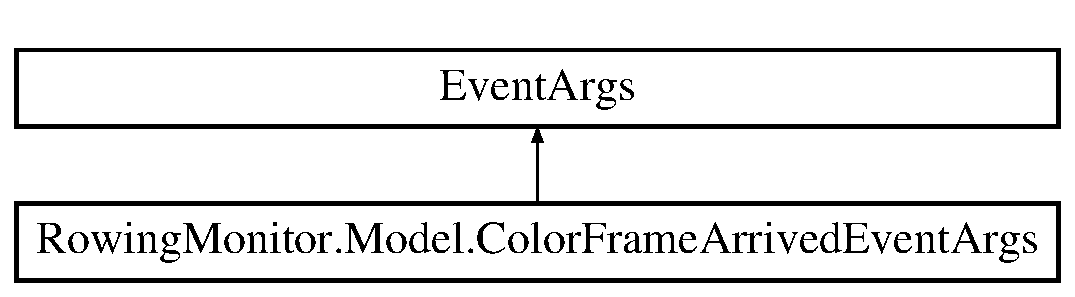
\includegraphics[height=2.000000cm]{class_rowing_monitor_1_1_model_1_1_color_frame_arrived_event_args}
\end{center}
\end{figure}
\subsection*{Public Member Functions}
\begin{DoxyCompactItemize}
\item 
\hyperlink{class_rowing_monitor_1_1_model_1_1_color_frame_arrived_event_args_a228785b0fda3657a17d7c30fd429ba1c}{Color\+Frame\+Arrived\+Event\+Args} (Writeable\+Bitmap color\+Bitmap)
\end{DoxyCompactItemize}
\subsection*{Properties}
\begin{DoxyCompactItemize}
\item 
Writeable\+Bitmap \hyperlink{class_rowing_monitor_1_1_model_1_1_color_frame_arrived_event_args_a2332327334320a56103d13596128a841}{Color\+Bitmap}\hspace{0.3cm}{\ttfamily  \mbox{[}get\mbox{]}}
\end{DoxyCompactItemize}


\subsection{Detailed Description}
Represents the arguments for a \hyperlink{class_rowing_monitor_1_1_model_1_1_kinect_reader}{Kinect\+Reader}\textquotesingle{}s Color\+Frame\+Arrived event. 



\subsection{Constructor \& Destructor Documentation}
\mbox{\Hypertarget{class_rowing_monitor_1_1_model_1_1_color_frame_arrived_event_args_a228785b0fda3657a17d7c30fd429ba1c}\label{class_rowing_monitor_1_1_model_1_1_color_frame_arrived_event_args_a228785b0fda3657a17d7c30fd429ba1c}} 
\index{Rowing\+Monitor\+::\+Model\+::\+Color\+Frame\+Arrived\+Event\+Args@{Rowing\+Monitor\+::\+Model\+::\+Color\+Frame\+Arrived\+Event\+Args}!Color\+Frame\+Arrived\+Event\+Args@{Color\+Frame\+Arrived\+Event\+Args}}
\index{Color\+Frame\+Arrived\+Event\+Args@{Color\+Frame\+Arrived\+Event\+Args}!Rowing\+Monitor\+::\+Model\+::\+Color\+Frame\+Arrived\+Event\+Args@{Rowing\+Monitor\+::\+Model\+::\+Color\+Frame\+Arrived\+Event\+Args}}
\subsubsection{\texorpdfstring{Color\+Frame\+Arrived\+Event\+Args()}{ColorFrameArrivedEventArgs()}}
{\footnotesize\ttfamily Rowing\+Monitor.\+Model.\+Color\+Frame\+Arrived\+Event\+Args.\+Color\+Frame\+Arrived\+Event\+Args (\begin{DoxyParamCaption}\item[{Writeable\+Bitmap}]{color\+Bitmap }\end{DoxyParamCaption})}



\subsection{Property Documentation}
\mbox{\Hypertarget{class_rowing_monitor_1_1_model_1_1_color_frame_arrived_event_args_a2332327334320a56103d13596128a841}\label{class_rowing_monitor_1_1_model_1_1_color_frame_arrived_event_args_a2332327334320a56103d13596128a841}} 
\index{Rowing\+Monitor\+::\+Model\+::\+Color\+Frame\+Arrived\+Event\+Args@{Rowing\+Monitor\+::\+Model\+::\+Color\+Frame\+Arrived\+Event\+Args}!Color\+Bitmap@{Color\+Bitmap}}
\index{Color\+Bitmap@{Color\+Bitmap}!Rowing\+Monitor\+::\+Model\+::\+Color\+Frame\+Arrived\+Event\+Args@{Rowing\+Monitor\+::\+Model\+::\+Color\+Frame\+Arrived\+Event\+Args}}
\subsubsection{\texorpdfstring{Color\+Bitmap}{ColorBitmap}}
{\footnotesize\ttfamily Writeable\+Bitmap Rowing\+Monitor.\+Model.\+Color\+Frame\+Arrived\+Event\+Args.\+Color\+Bitmap\hspace{0.3cm}{\ttfamily [get]}}



The documentation for this class was generated from the following file\+:\begin{DoxyCompactItemize}
\item 
Model/\+Event\+Args/\hyperlink{_color_frame_arrived_event_args_8cs}{Color\+Frame\+Arrived\+Event\+Args.\+cs}\end{DoxyCompactItemize}

\hypertarget{class_rowing_monitor_1_1_model_1_1_util_1_1_curve_fitting}{}\section{Rowing\+Monitor.\+Model.\+Util.\+Curve\+Fitting Class Reference}
\label{class_rowing_monitor_1_1_model_1_1_util_1_1_curve_fitting}\index{Rowing\+Monitor.\+Model.\+Util.\+Curve\+Fitting@{Rowing\+Monitor.\+Model.\+Util.\+Curve\+Fitting}}
\subsection*{Classes}
\begin{DoxyCompactItemize}
\item 
struct \hyperlink{struct_rowing_monitor_1_1_model_1_1_util_1_1_curve_fitting_1_1_quadratic_function_parameters}{Quadratic\+Function\+Parameters}
\end{DoxyCompactItemize}
\subsection*{Static Public Member Functions}
\begin{DoxyCompactItemize}
\item 
static \hyperlink{struct_rowing_monitor_1_1_model_1_1_util_1_1_curve_fitting_1_1_quadratic_function_parameters}{Quadratic\+Function\+Parameters} \hyperlink{class_rowing_monitor_1_1_model_1_1_util_1_1_curve_fitting_aab35f1296fc2b02ad4709abce8b52cf9}{Quadratic\+Function\+Fit} (double\mbox{[}$\,$\mbox{]} x, double\mbox{[}$\,$\mbox{]} y)
\item 
static double \hyperlink{class_rowing_monitor_1_1_model_1_1_util_1_1_curve_fitting_a0ce417f32d1e09fcceba1578a5955f3a}{Quadratic\+Function} (double x, double a, double b, double c)
\item 
static double \hyperlink{class_rowing_monitor_1_1_model_1_1_util_1_1_curve_fitting_a21bd155270e8abd871e52e400a896df0}{Quadratic\+Function} (double x, \hyperlink{struct_rowing_monitor_1_1_model_1_1_util_1_1_curve_fitting_1_1_quadratic_function_parameters}{Quadratic\+Function\+Parameters} param)
\end{DoxyCompactItemize}


\subsection{Member Function Documentation}
\mbox{\Hypertarget{class_rowing_monitor_1_1_model_1_1_util_1_1_curve_fitting_a0ce417f32d1e09fcceba1578a5955f3a}\label{class_rowing_monitor_1_1_model_1_1_util_1_1_curve_fitting_a0ce417f32d1e09fcceba1578a5955f3a}} 
\index{Rowing\+Monitor\+::\+Model\+::\+Util\+::\+Curve\+Fitting@{Rowing\+Monitor\+::\+Model\+::\+Util\+::\+Curve\+Fitting}!Quadratic\+Function@{Quadratic\+Function}}
\index{Quadratic\+Function@{Quadratic\+Function}!Rowing\+Monitor\+::\+Model\+::\+Util\+::\+Curve\+Fitting@{Rowing\+Monitor\+::\+Model\+::\+Util\+::\+Curve\+Fitting}}
\subsubsection{\texorpdfstring{Quadratic\+Function()}{QuadraticFunction()}\hspace{0.1cm}{\footnotesize\ttfamily [1/2]}}
{\footnotesize\ttfamily static double Rowing\+Monitor.\+Model.\+Util.\+Curve\+Fitting.\+Quadratic\+Function (\begin{DoxyParamCaption}\item[{double}]{x,  }\item[{double}]{a,  }\item[{double}]{b,  }\item[{double}]{c }\end{DoxyParamCaption})\hspace{0.3cm}{\ttfamily [static]}}

\mbox{\Hypertarget{class_rowing_monitor_1_1_model_1_1_util_1_1_curve_fitting_a21bd155270e8abd871e52e400a896df0}\label{class_rowing_monitor_1_1_model_1_1_util_1_1_curve_fitting_a21bd155270e8abd871e52e400a896df0}} 
\index{Rowing\+Monitor\+::\+Model\+::\+Util\+::\+Curve\+Fitting@{Rowing\+Monitor\+::\+Model\+::\+Util\+::\+Curve\+Fitting}!Quadratic\+Function@{Quadratic\+Function}}
\index{Quadratic\+Function@{Quadratic\+Function}!Rowing\+Monitor\+::\+Model\+::\+Util\+::\+Curve\+Fitting@{Rowing\+Monitor\+::\+Model\+::\+Util\+::\+Curve\+Fitting}}
\subsubsection{\texorpdfstring{Quadratic\+Function()}{QuadraticFunction()}\hspace{0.1cm}{\footnotesize\ttfamily [2/2]}}
{\footnotesize\ttfamily static double Rowing\+Monitor.\+Model.\+Util.\+Curve\+Fitting.\+Quadratic\+Function (\begin{DoxyParamCaption}\item[{double}]{x,  }\item[{\hyperlink{struct_rowing_monitor_1_1_model_1_1_util_1_1_curve_fitting_1_1_quadratic_function_parameters}{Quadratic\+Function\+Parameters}}]{param }\end{DoxyParamCaption})\hspace{0.3cm}{\ttfamily [static]}}

\mbox{\Hypertarget{class_rowing_monitor_1_1_model_1_1_util_1_1_curve_fitting_aab35f1296fc2b02ad4709abce8b52cf9}\label{class_rowing_monitor_1_1_model_1_1_util_1_1_curve_fitting_aab35f1296fc2b02ad4709abce8b52cf9}} 
\index{Rowing\+Monitor\+::\+Model\+::\+Util\+::\+Curve\+Fitting@{Rowing\+Monitor\+::\+Model\+::\+Util\+::\+Curve\+Fitting}!Quadratic\+Function\+Fit@{Quadratic\+Function\+Fit}}
\index{Quadratic\+Function\+Fit@{Quadratic\+Function\+Fit}!Rowing\+Monitor\+::\+Model\+::\+Util\+::\+Curve\+Fitting@{Rowing\+Monitor\+::\+Model\+::\+Util\+::\+Curve\+Fitting}}
\subsubsection{\texorpdfstring{Quadratic\+Function\+Fit()}{QuadraticFunctionFit()}}
{\footnotesize\ttfamily static \hyperlink{struct_rowing_monitor_1_1_model_1_1_util_1_1_curve_fitting_1_1_quadratic_function_parameters}{Quadratic\+Function\+Parameters} Rowing\+Monitor.\+Model.\+Util.\+Curve\+Fitting.\+Quadratic\+Function\+Fit (\begin{DoxyParamCaption}\item[{double \mbox{[}$\,$\mbox{]}}]{x,  }\item[{double \mbox{[}$\,$\mbox{]}}]{y }\end{DoxyParamCaption})\hspace{0.3cm}{\ttfamily [static]}}



The documentation for this class was generated from the following file\+:\begin{DoxyCompactItemize}
\item 
Model/\+Util/\hyperlink{_curve_fitting_8cs}{Curve\+Fitting.\+cs}\end{DoxyCompactItemize}

\hypertarget{class_rowing_monitor_1_1_view_1_1_debug_view}{}\section{Rowing\+Monitor.\+View.\+Debug\+View Class Reference}
\label{class_rowing_monitor_1_1_view_1_1_debug_view}\index{Rowing\+Monitor.\+View.\+Debug\+View@{Rowing\+Monitor.\+View.\+Debug\+View}}


\hyperlink{class_rowing_monitor_1_1_view_1_1_debug_view}{Debug\+View}  


Inheritance diagram for Rowing\+Monitor.\+View.\+Debug\+View\+:\begin{figure}[H]
\begin{center}
\leavevmode
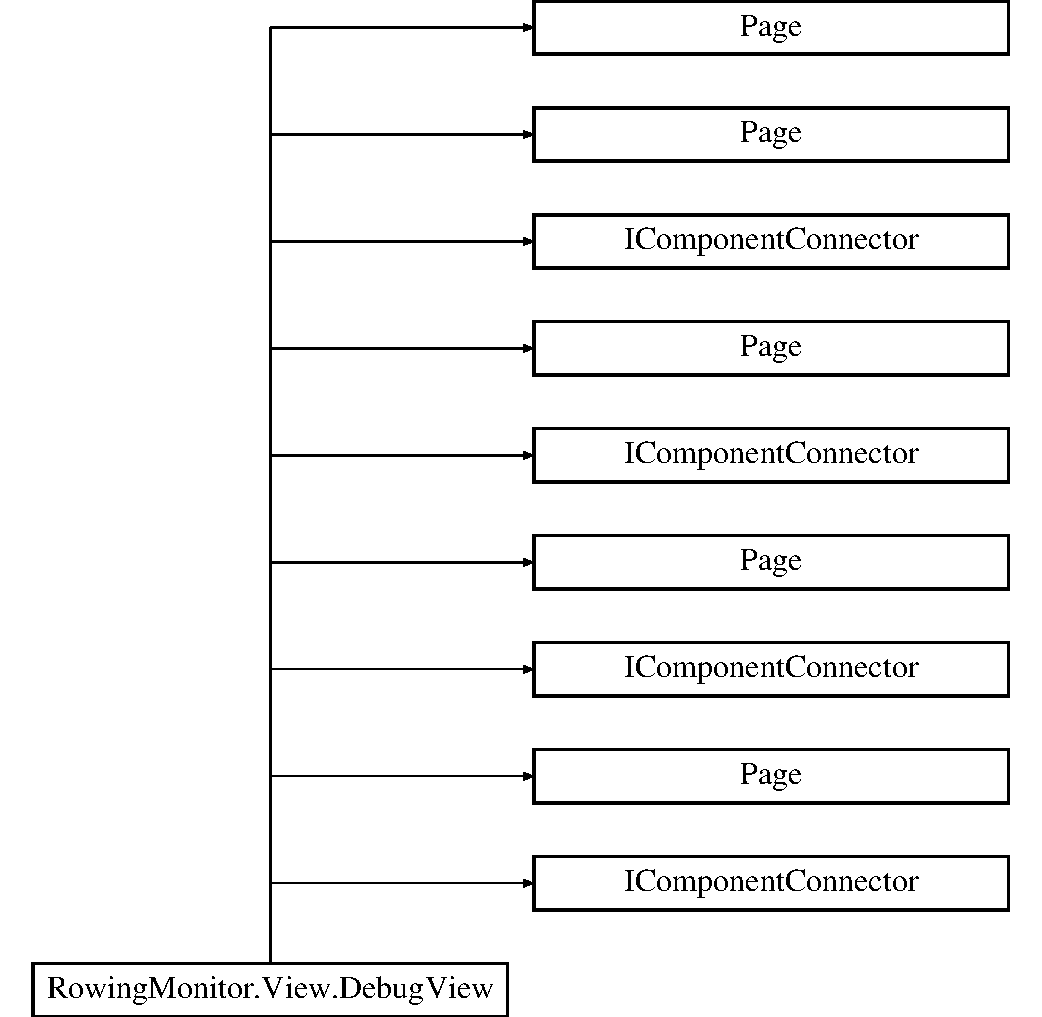
\includegraphics[height=10.000000cm]{class_rowing_monitor_1_1_view_1_1_debug_view}
\end{center}
\end{figure}
\subsection*{Public Member Functions}
\begin{DoxyCompactItemize}
\item 
void \hyperlink{class_rowing_monitor_1_1_view_1_1_debug_view_a3fd59a2688428b98569c4fc149657a70}{Initialize\+Component} ()
\begin{DoxyCompactList}\small\item\em Initialize\+Component \end{DoxyCompactList}\item 
void \hyperlink{class_rowing_monitor_1_1_view_1_1_debug_view_a3fd59a2688428b98569c4fc149657a70}{Initialize\+Component} ()
\begin{DoxyCompactList}\small\item\em Initialize\+Component \end{DoxyCompactList}\item 
void \hyperlink{class_rowing_monitor_1_1_view_1_1_debug_view_a3fd59a2688428b98569c4fc149657a70}{Initialize\+Component} ()
\begin{DoxyCompactList}\small\item\em Initialize\+Component \end{DoxyCompactList}\item 
void \hyperlink{class_rowing_monitor_1_1_view_1_1_debug_view_a3fd59a2688428b98569c4fc149657a70}{Initialize\+Component} ()
\begin{DoxyCompactList}\small\item\em Initialize\+Component \end{DoxyCompactList}\item 
\hyperlink{class_rowing_monitor_1_1_view_1_1_debug_view_a6fed59204b8250cd7d7af0a932c78394}{Debug\+View} ()
\end{DoxyCompactItemize}


\subsection{Detailed Description}
\hyperlink{class_rowing_monitor_1_1_view_1_1_debug_view}{Debug\+View} 

Interaktionslogik für Rowing\+Monitor\+Window.\+xaml 

\subsection{Constructor \& Destructor Documentation}
\mbox{\Hypertarget{class_rowing_monitor_1_1_view_1_1_debug_view_a6fed59204b8250cd7d7af0a932c78394}\label{class_rowing_monitor_1_1_view_1_1_debug_view_a6fed59204b8250cd7d7af0a932c78394}} 
\index{Rowing\+Monitor\+::\+View\+::\+Debug\+View@{Rowing\+Monitor\+::\+View\+::\+Debug\+View}!Debug\+View@{Debug\+View}}
\index{Debug\+View@{Debug\+View}!Rowing\+Monitor\+::\+View\+::\+Debug\+View@{Rowing\+Monitor\+::\+View\+::\+Debug\+View}}
\subsubsection{\texorpdfstring{Debug\+View()}{DebugView()}}
{\footnotesize\ttfamily Rowing\+Monitor.\+View.\+Debug\+View.\+Debug\+View (\begin{DoxyParamCaption}{ }\end{DoxyParamCaption})}



\subsection{Member Function Documentation}
\mbox{\Hypertarget{class_rowing_monitor_1_1_view_1_1_debug_view_a3fd59a2688428b98569c4fc149657a70}\label{class_rowing_monitor_1_1_view_1_1_debug_view_a3fd59a2688428b98569c4fc149657a70}} 
\index{Rowing\+Monitor\+::\+View\+::\+Debug\+View@{Rowing\+Monitor\+::\+View\+::\+Debug\+View}!Initialize\+Component@{Initialize\+Component}}
\index{Initialize\+Component@{Initialize\+Component}!Rowing\+Monitor\+::\+View\+::\+Debug\+View@{Rowing\+Monitor\+::\+View\+::\+Debug\+View}}
\subsubsection{\texorpdfstring{Initialize\+Component()}{InitializeComponent()}\hspace{0.1cm}{\footnotesize\ttfamily [1/4]}}
{\footnotesize\ttfamily void Rowing\+Monitor.\+View.\+Debug\+View.\+Initialize\+Component (\begin{DoxyParamCaption}{ }\end{DoxyParamCaption})}



Initialize\+Component 

\mbox{\Hypertarget{class_rowing_monitor_1_1_view_1_1_debug_view_a3fd59a2688428b98569c4fc149657a70}\label{class_rowing_monitor_1_1_view_1_1_debug_view_a3fd59a2688428b98569c4fc149657a70}} 
\index{Rowing\+Monitor\+::\+View\+::\+Debug\+View@{Rowing\+Monitor\+::\+View\+::\+Debug\+View}!Initialize\+Component@{Initialize\+Component}}
\index{Initialize\+Component@{Initialize\+Component}!Rowing\+Monitor\+::\+View\+::\+Debug\+View@{Rowing\+Monitor\+::\+View\+::\+Debug\+View}}
\subsubsection{\texorpdfstring{Initialize\+Component()}{InitializeComponent()}\hspace{0.1cm}{\footnotesize\ttfamily [2/4]}}
{\footnotesize\ttfamily void Rowing\+Monitor.\+View.\+Debug\+View.\+Initialize\+Component (\begin{DoxyParamCaption}{ }\end{DoxyParamCaption})}



Initialize\+Component 

\mbox{\Hypertarget{class_rowing_monitor_1_1_view_1_1_debug_view_a3fd59a2688428b98569c4fc149657a70}\label{class_rowing_monitor_1_1_view_1_1_debug_view_a3fd59a2688428b98569c4fc149657a70}} 
\index{Rowing\+Monitor\+::\+View\+::\+Debug\+View@{Rowing\+Monitor\+::\+View\+::\+Debug\+View}!Initialize\+Component@{Initialize\+Component}}
\index{Initialize\+Component@{Initialize\+Component}!Rowing\+Monitor\+::\+View\+::\+Debug\+View@{Rowing\+Monitor\+::\+View\+::\+Debug\+View}}
\subsubsection{\texorpdfstring{Initialize\+Component()}{InitializeComponent()}\hspace{0.1cm}{\footnotesize\ttfamily [3/4]}}
{\footnotesize\ttfamily void Rowing\+Monitor.\+View.\+Debug\+View.\+Initialize\+Component (\begin{DoxyParamCaption}{ }\end{DoxyParamCaption})}



Initialize\+Component 

\mbox{\Hypertarget{class_rowing_monitor_1_1_view_1_1_debug_view_a3fd59a2688428b98569c4fc149657a70}\label{class_rowing_monitor_1_1_view_1_1_debug_view_a3fd59a2688428b98569c4fc149657a70}} 
\index{Rowing\+Monitor\+::\+View\+::\+Debug\+View@{Rowing\+Monitor\+::\+View\+::\+Debug\+View}!Initialize\+Component@{Initialize\+Component}}
\index{Initialize\+Component@{Initialize\+Component}!Rowing\+Monitor\+::\+View\+::\+Debug\+View@{Rowing\+Monitor\+::\+View\+::\+Debug\+View}}
\subsubsection{\texorpdfstring{Initialize\+Component()}{InitializeComponent()}\hspace{0.1cm}{\footnotesize\ttfamily [4/4]}}
{\footnotesize\ttfamily void Rowing\+Monitor.\+View.\+Debug\+View.\+Initialize\+Component (\begin{DoxyParamCaption}{ }\end{DoxyParamCaption})}



Initialize\+Component 



The documentation for this class was generated from the following files\+:\begin{DoxyCompactItemize}
\item 
obj/\+Debug/\+View/\hyperlink{_debug_2_view_2_debug_view_8g_8cs}{Debug\+View.\+g.\+cs}\item 
obj/\+Debug/\+View/\hyperlink{_debug_2_view_2_debug_view_8g_8i_8cs}{Debug\+View.\+g.\+i.\+cs}\item 
View/\hyperlink{_debug_view_8xaml_8cs}{Debug\+View.\+xaml.\+cs}\end{DoxyCompactItemize}

\hypertarget{class_rowing_monitor_1_1_view_model_1_1_debug_view_model}{}\section{Rowing\+Monitor.\+View\+Model.\+Debug\+View\+Model Class Reference}
\label{class_rowing_monitor_1_1_view_model_1_1_debug_view_model}\index{Rowing\+Monitor.\+View\+Model.\+Debug\+View\+Model@{Rowing\+Monitor.\+View\+Model.\+Debug\+View\+Model}}
\subsection*{Public Member Functions}
\begin{DoxyCompactItemize}
\item 
\hyperlink{class_rowing_monitor_1_1_view_model_1_1_debug_view_model_a9a09d0e5bcf1e919b8bff6fd9e7bc446}{Debug\+View\+Model} ()
\item 
void \hyperlink{class_rowing_monitor_1_1_view_model_1_1_debug_view_model_ac98ef68bcbe80ff74e742877c0bad04a}{View\+Loaded} ()
\item 
void \hyperlink{class_rowing_monitor_1_1_view_model_1_1_debug_view_model_ad8fab68504357f6e002e8a3e8ef0522b}{View\+Unloaded} ()
\item 
void \hyperlink{class_rowing_monitor_1_1_view_model_1_1_debug_view_model_a13676053f64717dc6e3dded15b158016}{Change\+Segment\+Detector} ()
\item 
void \hyperlink{class_rowing_monitor_1_1_view_model_1_1_debug_view_model_a874acc432d71f1cc9118ff8fda71a2f6}{Change\+Smoothing\+Filter} ()
\end{DoxyCompactItemize}
\subsection*{Properties}
\begin{DoxyCompactItemize}
\item 
List$<$ Joint\+Type $>$ \hyperlink{class_rowing_monitor_1_1_view_model_1_1_debug_view_model_a41dc4f6035874ac84cf7e184d55786b5}{Plot\+Joint\+Types}\hspace{0.3cm}{\ttfamily  \mbox{[}get, set\mbox{]}}
\item 
List$<$ \hyperlink{namespace_rowing_monitor_1_1_model_1_1_util_a01e1a06061533b246feb7421c9d0107f}{Data\+Stream\+Type} $>$ \hyperlink{class_rowing_monitor_1_1_view_model_1_1_debug_view_model_adeea14566ca983399b9258a6d11ccd94}{Plot\+Measured\+Variables}\hspace{0.3cm}{\ttfamily  \mbox{[}get, set\mbox{]}}
\item 
bool \hyperlink{class_rowing_monitor_1_1_view_model_1_1_debug_view_model_a6b953c4498e5cf1bbe866176f2bcc194}{Use\+Kinect\+Joint\+Filter}\hspace{0.3cm}{\ttfamily  \mbox{[}get, set\mbox{]}}
\item 
bool \hyperlink{class_rowing_monitor_1_1_view_model_1_1_debug_view_model_a9d8e1ac2c56509c97522a409f3c87db1}{Use\+Z\+VC}\hspace{0.3cm}{\ttfamily  \mbox{[}get, set\mbox{]}}
\item 
float \hyperlink{class_rowing_monitor_1_1_view_model_1_1_debug_view_model_a3c5a6901e5cfe6d6ca2ea49f6939cc5e}{Plot\+Range}\hspace{0.3cm}{\ttfamily  \mbox{[}get, set\mbox{]}}
\item 
Grid \hyperlink{class_rowing_monitor_1_1_view_model_1_1_debug_view_model_a7ab2d29ceb37f0650a15ee6c32401c3f}{Grid}\hspace{0.3cm}{\ttfamily  \mbox{[}get, set\mbox{]}}
\item 
float \hyperlink{class_rowing_monitor_1_1_view_model_1_1_debug_view_model_a6945ae46c3ce1f69f39fdbdb90ae1d66}{Kleshnev\+Plot\+Range}\hspace{0.3cm}{\ttfamily  \mbox{[}get, set\mbox{]}}
\end{DoxyCompactItemize}


\subsection{Constructor \& Destructor Documentation}
\mbox{\Hypertarget{class_rowing_monitor_1_1_view_model_1_1_debug_view_model_a9a09d0e5bcf1e919b8bff6fd9e7bc446}\label{class_rowing_monitor_1_1_view_model_1_1_debug_view_model_a9a09d0e5bcf1e919b8bff6fd9e7bc446}} 
\index{Rowing\+Monitor\+::\+View\+Model\+::\+Debug\+View\+Model@{Rowing\+Monitor\+::\+View\+Model\+::\+Debug\+View\+Model}!Debug\+View\+Model@{Debug\+View\+Model}}
\index{Debug\+View\+Model@{Debug\+View\+Model}!Rowing\+Monitor\+::\+View\+Model\+::\+Debug\+View\+Model@{Rowing\+Monitor\+::\+View\+Model\+::\+Debug\+View\+Model}}
\subsubsection{\texorpdfstring{Debug\+View\+Model()}{DebugViewModel()}}
{\footnotesize\ttfamily Rowing\+Monitor.\+View\+Model.\+Debug\+View\+Model.\+Debug\+View\+Model (\begin{DoxyParamCaption}{ }\end{DoxyParamCaption})}



\subsection{Member Function Documentation}
\mbox{\Hypertarget{class_rowing_monitor_1_1_view_model_1_1_debug_view_model_a13676053f64717dc6e3dded15b158016}\label{class_rowing_monitor_1_1_view_model_1_1_debug_view_model_a13676053f64717dc6e3dded15b158016}} 
\index{Rowing\+Monitor\+::\+View\+Model\+::\+Debug\+View\+Model@{Rowing\+Monitor\+::\+View\+Model\+::\+Debug\+View\+Model}!Change\+Segment\+Detector@{Change\+Segment\+Detector}}
\index{Change\+Segment\+Detector@{Change\+Segment\+Detector}!Rowing\+Monitor\+::\+View\+Model\+::\+Debug\+View\+Model@{Rowing\+Monitor\+::\+View\+Model\+::\+Debug\+View\+Model}}
\subsubsection{\texorpdfstring{Change\+Segment\+Detector()}{ChangeSegmentDetector()}}
{\footnotesize\ttfamily void Rowing\+Monitor.\+View\+Model.\+Debug\+View\+Model.\+Change\+Segment\+Detector (\begin{DoxyParamCaption}{ }\end{DoxyParamCaption})}

\mbox{\Hypertarget{class_rowing_monitor_1_1_view_model_1_1_debug_view_model_a874acc432d71f1cc9118ff8fda71a2f6}\label{class_rowing_monitor_1_1_view_model_1_1_debug_view_model_a874acc432d71f1cc9118ff8fda71a2f6}} 
\index{Rowing\+Monitor\+::\+View\+Model\+::\+Debug\+View\+Model@{Rowing\+Monitor\+::\+View\+Model\+::\+Debug\+View\+Model}!Change\+Smoothing\+Filter@{Change\+Smoothing\+Filter}}
\index{Change\+Smoothing\+Filter@{Change\+Smoothing\+Filter}!Rowing\+Monitor\+::\+View\+Model\+::\+Debug\+View\+Model@{Rowing\+Monitor\+::\+View\+Model\+::\+Debug\+View\+Model}}
\subsubsection{\texorpdfstring{Change\+Smoothing\+Filter()}{ChangeSmoothingFilter()}}
{\footnotesize\ttfamily void Rowing\+Monitor.\+View\+Model.\+Debug\+View\+Model.\+Change\+Smoothing\+Filter (\begin{DoxyParamCaption}{ }\end{DoxyParamCaption})}

\mbox{\Hypertarget{class_rowing_monitor_1_1_view_model_1_1_debug_view_model_ac98ef68bcbe80ff74e742877c0bad04a}\label{class_rowing_monitor_1_1_view_model_1_1_debug_view_model_ac98ef68bcbe80ff74e742877c0bad04a}} 
\index{Rowing\+Monitor\+::\+View\+Model\+::\+Debug\+View\+Model@{Rowing\+Monitor\+::\+View\+Model\+::\+Debug\+View\+Model}!View\+Loaded@{View\+Loaded}}
\index{View\+Loaded@{View\+Loaded}!Rowing\+Monitor\+::\+View\+Model\+::\+Debug\+View\+Model@{Rowing\+Monitor\+::\+View\+Model\+::\+Debug\+View\+Model}}
\subsubsection{\texorpdfstring{View\+Loaded()}{ViewLoaded()}}
{\footnotesize\ttfamily void Rowing\+Monitor.\+View\+Model.\+Debug\+View\+Model.\+View\+Loaded (\begin{DoxyParamCaption}{ }\end{DoxyParamCaption})}

\mbox{\Hypertarget{class_rowing_monitor_1_1_view_model_1_1_debug_view_model_ad8fab68504357f6e002e8a3e8ef0522b}\label{class_rowing_monitor_1_1_view_model_1_1_debug_view_model_ad8fab68504357f6e002e8a3e8ef0522b}} 
\index{Rowing\+Monitor\+::\+View\+Model\+::\+Debug\+View\+Model@{Rowing\+Monitor\+::\+View\+Model\+::\+Debug\+View\+Model}!View\+Unloaded@{View\+Unloaded}}
\index{View\+Unloaded@{View\+Unloaded}!Rowing\+Monitor\+::\+View\+Model\+::\+Debug\+View\+Model@{Rowing\+Monitor\+::\+View\+Model\+::\+Debug\+View\+Model}}
\subsubsection{\texorpdfstring{View\+Unloaded()}{ViewUnloaded()}}
{\footnotesize\ttfamily void Rowing\+Monitor.\+View\+Model.\+Debug\+View\+Model.\+View\+Unloaded (\begin{DoxyParamCaption}{ }\end{DoxyParamCaption})}



\subsection{Property Documentation}
\mbox{\Hypertarget{class_rowing_monitor_1_1_view_model_1_1_debug_view_model_a7ab2d29ceb37f0650a15ee6c32401c3f}\label{class_rowing_monitor_1_1_view_model_1_1_debug_view_model_a7ab2d29ceb37f0650a15ee6c32401c3f}} 
\index{Rowing\+Monitor\+::\+View\+Model\+::\+Debug\+View\+Model@{Rowing\+Monitor\+::\+View\+Model\+::\+Debug\+View\+Model}!Grid@{Grid}}
\index{Grid@{Grid}!Rowing\+Monitor\+::\+View\+Model\+::\+Debug\+View\+Model@{Rowing\+Monitor\+::\+View\+Model\+::\+Debug\+View\+Model}}
\subsubsection{\texorpdfstring{Grid}{Grid}}
{\footnotesize\ttfamily Grid Rowing\+Monitor.\+View\+Model.\+Debug\+View\+Model.\+Grid\hspace{0.3cm}{\ttfamily [get]}, {\ttfamily [set]}}

\mbox{\Hypertarget{class_rowing_monitor_1_1_view_model_1_1_debug_view_model_a6945ae46c3ce1f69f39fdbdb90ae1d66}\label{class_rowing_monitor_1_1_view_model_1_1_debug_view_model_a6945ae46c3ce1f69f39fdbdb90ae1d66}} 
\index{Rowing\+Monitor\+::\+View\+Model\+::\+Debug\+View\+Model@{Rowing\+Monitor\+::\+View\+Model\+::\+Debug\+View\+Model}!Kleshnev\+Plot\+Range@{Kleshnev\+Plot\+Range}}
\index{Kleshnev\+Plot\+Range@{Kleshnev\+Plot\+Range}!Rowing\+Monitor\+::\+View\+Model\+::\+Debug\+View\+Model@{Rowing\+Monitor\+::\+View\+Model\+::\+Debug\+View\+Model}}
\subsubsection{\texorpdfstring{Kleshnev\+Plot\+Range}{KleshnevPlotRange}}
{\footnotesize\ttfamily float Rowing\+Monitor.\+View\+Model.\+Debug\+View\+Model.\+Kleshnev\+Plot\+Range\hspace{0.3cm}{\ttfamily [get]}, {\ttfamily [set]}}

\mbox{\Hypertarget{class_rowing_monitor_1_1_view_model_1_1_debug_view_model_a41dc4f6035874ac84cf7e184d55786b5}\label{class_rowing_monitor_1_1_view_model_1_1_debug_view_model_a41dc4f6035874ac84cf7e184d55786b5}} 
\index{Rowing\+Monitor\+::\+View\+Model\+::\+Debug\+View\+Model@{Rowing\+Monitor\+::\+View\+Model\+::\+Debug\+View\+Model}!Plot\+Joint\+Types@{Plot\+Joint\+Types}}
\index{Plot\+Joint\+Types@{Plot\+Joint\+Types}!Rowing\+Monitor\+::\+View\+Model\+::\+Debug\+View\+Model@{Rowing\+Monitor\+::\+View\+Model\+::\+Debug\+View\+Model}}
\subsubsection{\texorpdfstring{Plot\+Joint\+Types}{PlotJointTypes}}
{\footnotesize\ttfamily List$<$Joint\+Type$>$ Rowing\+Monitor.\+View\+Model.\+Debug\+View\+Model.\+Plot\+Joint\+Types\hspace{0.3cm}{\ttfamily [get]}, {\ttfamily [set]}}

\mbox{\Hypertarget{class_rowing_monitor_1_1_view_model_1_1_debug_view_model_adeea14566ca983399b9258a6d11ccd94}\label{class_rowing_monitor_1_1_view_model_1_1_debug_view_model_adeea14566ca983399b9258a6d11ccd94}} 
\index{Rowing\+Monitor\+::\+View\+Model\+::\+Debug\+View\+Model@{Rowing\+Monitor\+::\+View\+Model\+::\+Debug\+View\+Model}!Plot\+Measured\+Variables@{Plot\+Measured\+Variables}}
\index{Plot\+Measured\+Variables@{Plot\+Measured\+Variables}!Rowing\+Monitor\+::\+View\+Model\+::\+Debug\+View\+Model@{Rowing\+Monitor\+::\+View\+Model\+::\+Debug\+View\+Model}}
\subsubsection{\texorpdfstring{Plot\+Measured\+Variables}{PlotMeasuredVariables}}
{\footnotesize\ttfamily List$<$\hyperlink{namespace_rowing_monitor_1_1_model_1_1_util_a01e1a06061533b246feb7421c9d0107f}{Data\+Stream\+Type}$>$ Rowing\+Monitor.\+View\+Model.\+Debug\+View\+Model.\+Plot\+Measured\+Variables\hspace{0.3cm}{\ttfamily [get]}, {\ttfamily [set]}}

\mbox{\Hypertarget{class_rowing_monitor_1_1_view_model_1_1_debug_view_model_a3c5a6901e5cfe6d6ca2ea49f6939cc5e}\label{class_rowing_monitor_1_1_view_model_1_1_debug_view_model_a3c5a6901e5cfe6d6ca2ea49f6939cc5e}} 
\index{Rowing\+Monitor\+::\+View\+Model\+::\+Debug\+View\+Model@{Rowing\+Monitor\+::\+View\+Model\+::\+Debug\+View\+Model}!Plot\+Range@{Plot\+Range}}
\index{Plot\+Range@{Plot\+Range}!Rowing\+Monitor\+::\+View\+Model\+::\+Debug\+View\+Model@{Rowing\+Monitor\+::\+View\+Model\+::\+Debug\+View\+Model}}
\subsubsection{\texorpdfstring{Plot\+Range}{PlotRange}}
{\footnotesize\ttfamily float Rowing\+Monitor.\+View\+Model.\+Debug\+View\+Model.\+Plot\+Range\hspace{0.3cm}{\ttfamily [get]}, {\ttfamily [set]}}

\mbox{\Hypertarget{class_rowing_monitor_1_1_view_model_1_1_debug_view_model_a6b953c4498e5cf1bbe866176f2bcc194}\label{class_rowing_monitor_1_1_view_model_1_1_debug_view_model_a6b953c4498e5cf1bbe866176f2bcc194}} 
\index{Rowing\+Monitor\+::\+View\+Model\+::\+Debug\+View\+Model@{Rowing\+Monitor\+::\+View\+Model\+::\+Debug\+View\+Model}!Use\+Kinect\+Joint\+Filter@{Use\+Kinect\+Joint\+Filter}}
\index{Use\+Kinect\+Joint\+Filter@{Use\+Kinect\+Joint\+Filter}!Rowing\+Monitor\+::\+View\+Model\+::\+Debug\+View\+Model@{Rowing\+Monitor\+::\+View\+Model\+::\+Debug\+View\+Model}}
\subsubsection{\texorpdfstring{Use\+Kinect\+Joint\+Filter}{UseKinectJointFilter}}
{\footnotesize\ttfamily bool Rowing\+Monitor.\+View\+Model.\+Debug\+View\+Model.\+Use\+Kinect\+Joint\+Filter\hspace{0.3cm}{\ttfamily [get]}, {\ttfamily [set]}}

\mbox{\Hypertarget{class_rowing_monitor_1_1_view_model_1_1_debug_view_model_a9d8e1ac2c56509c97522a409f3c87db1}\label{class_rowing_monitor_1_1_view_model_1_1_debug_view_model_a9d8e1ac2c56509c97522a409f3c87db1}} 
\index{Rowing\+Monitor\+::\+View\+Model\+::\+Debug\+View\+Model@{Rowing\+Monitor\+::\+View\+Model\+::\+Debug\+View\+Model}!Use\+Z\+VC@{Use\+Z\+VC}}
\index{Use\+Z\+VC@{Use\+Z\+VC}!Rowing\+Monitor\+::\+View\+Model\+::\+Debug\+View\+Model@{Rowing\+Monitor\+::\+View\+Model\+::\+Debug\+View\+Model}}
\subsubsection{\texorpdfstring{Use\+Z\+VC}{UseZVC}}
{\footnotesize\ttfamily bool Rowing\+Monitor.\+View\+Model.\+Debug\+View\+Model.\+Use\+Z\+VC\hspace{0.3cm}{\ttfamily [get]}, {\ttfamily [set]}}



The documentation for this class was generated from the following file\+:\begin{DoxyCompactItemize}
\item 
View\+Model/\hyperlink{_debug_view_model_8cs}{Debug\+View\+Model.\+cs}\end{DoxyCompactItemize}

\hypertarget{class_rowing_monitor_1_1_model_1_1_util_1_1_degrees}{}\section{Rowing\+Monitor.\+Model.\+Util.\+Degrees Class Reference}
\label{class_rowing_monitor_1_1_model_1_1_util_1_1_degrees}\index{Rowing\+Monitor.\+Model.\+Util.\+Degrees@{Rowing\+Monitor.\+Model.\+Util.\+Degrees}}
\subsection*{Static Public Member Functions}
\begin{DoxyCompactItemize}
\item 
static double \hyperlink{class_rowing_monitor_1_1_model_1_1_util_1_1_degrees_a8d8da87b6f4f265742c46c1bca007819}{Degree\+To\+Radian} (double angle)
\item 
static double \hyperlink{class_rowing_monitor_1_1_model_1_1_util_1_1_degrees_aebe42221859cd2b97603d00bfc0e7c6c}{Radian\+To\+Degree} (double angle)
\end{DoxyCompactItemize}


\subsection{Member Function Documentation}
\mbox{\Hypertarget{class_rowing_monitor_1_1_model_1_1_util_1_1_degrees_a8d8da87b6f4f265742c46c1bca007819}\label{class_rowing_monitor_1_1_model_1_1_util_1_1_degrees_a8d8da87b6f4f265742c46c1bca007819}} 
\index{Rowing\+Monitor\+::\+Model\+::\+Util\+::\+Degrees@{Rowing\+Monitor\+::\+Model\+::\+Util\+::\+Degrees}!Degree\+To\+Radian@{Degree\+To\+Radian}}
\index{Degree\+To\+Radian@{Degree\+To\+Radian}!Rowing\+Monitor\+::\+Model\+::\+Util\+::\+Degrees@{Rowing\+Monitor\+::\+Model\+::\+Util\+::\+Degrees}}
\subsubsection{\texorpdfstring{Degree\+To\+Radian()}{DegreeToRadian()}}
{\footnotesize\ttfamily static double Rowing\+Monitor.\+Model.\+Util.\+Degrees.\+Degree\+To\+Radian (\begin{DoxyParamCaption}\item[{double}]{angle }\end{DoxyParamCaption})\hspace{0.3cm}{\ttfamily [static]}}

\mbox{\Hypertarget{class_rowing_monitor_1_1_model_1_1_util_1_1_degrees_aebe42221859cd2b97603d00bfc0e7c6c}\label{class_rowing_monitor_1_1_model_1_1_util_1_1_degrees_aebe42221859cd2b97603d00bfc0e7c6c}} 
\index{Rowing\+Monitor\+::\+Model\+::\+Util\+::\+Degrees@{Rowing\+Monitor\+::\+Model\+::\+Util\+::\+Degrees}!Radian\+To\+Degree@{Radian\+To\+Degree}}
\index{Radian\+To\+Degree@{Radian\+To\+Degree}!Rowing\+Monitor\+::\+Model\+::\+Util\+::\+Degrees@{Rowing\+Monitor\+::\+Model\+::\+Util\+::\+Degrees}}
\subsubsection{\texorpdfstring{Radian\+To\+Degree()}{RadianToDegree()}}
{\footnotesize\ttfamily static double Rowing\+Monitor.\+Model.\+Util.\+Degrees.\+Radian\+To\+Degree (\begin{DoxyParamCaption}\item[{double}]{angle }\end{DoxyParamCaption})\hspace{0.3cm}{\ttfamily [static]}}



The documentation for this class was generated from the following file\+:\begin{DoxyCompactItemize}
\item 
Model/\+Util/\hyperlink{_degrees_8cs}{Degrees.\+cs}\end{DoxyCompactItemize}

\hypertarget{class_rowing_monitor_1_1_model_1_1_pipeline_1_1_d_t_w_segment_detector}{}\section{Rowing\+Monitor.\+Model.\+Pipeline.\+D\+T\+W\+Segment\+Detector Class Reference}
\label{class_rowing_monitor_1_1_model_1_1_pipeline_1_1_d_t_w_segment_detector}\index{Rowing\+Monitor.\+Model.\+Pipeline.\+D\+T\+W\+Segment\+Detector@{Rowing\+Monitor.\+Model.\+Pipeline.\+D\+T\+W\+Segment\+Detector}}
Inheritance diagram for Rowing\+Monitor.\+Model.\+Pipeline.\+D\+T\+W\+Segment\+Detector\+:\begin{figure}[H]
\begin{center}
\leavevmode
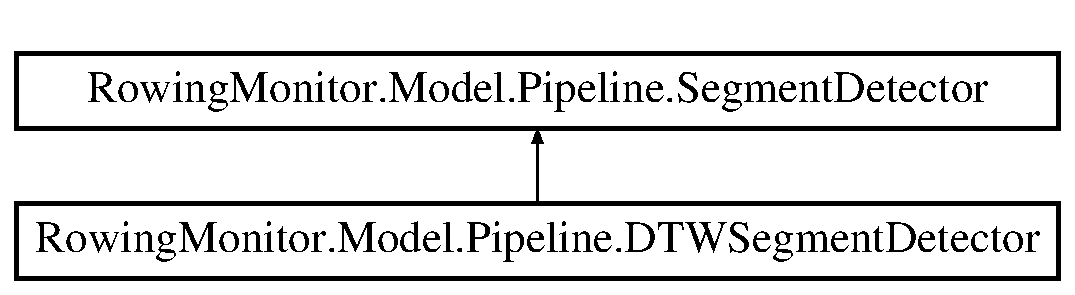
\includegraphics[height=2.000000cm]{class_rowing_monitor_1_1_model_1_1_pipeline_1_1_d_t_w_segment_detector}
\end{center}
\end{figure}
\subsection*{Public Member Functions}
\begin{DoxyCompactItemize}
\item 
\hyperlink{class_rowing_monitor_1_1_model_1_1_pipeline_1_1_d_t_w_segment_detector_abfb0a6199eaaf5bb079bbcf1c2eaecc5}{D\+T\+W\+Segment\+Detector} (float distance\+Threshold, int minimum\+Subsequence\+Length)
\item 
override void \hyperlink{class_rowing_monitor_1_1_model_1_1_pipeline_1_1_d_t_w_segment_detector_a211aec92693f8a229d88dd6a5b059eb4}{Update} (\hyperlink{struct_rowing_monitor_1_1_model_1_1_util_1_1_joint_data}{Joint\+Data} joint\+Data, Joint\+Type joint\+Type, string axis)
\item 
override List$<$ \hyperlink{struct_rowing_monitor_1_1_model_1_1_util_1_1_segment_hit}{Segment\+Hit} $>$ \hyperlink{class_rowing_monitor_1_1_model_1_1_pipeline_1_1_d_t_w_segment_detector_ab65c258b405b4a73e22ea114173965a6}{Detect} (\hyperlink{struct_rowing_monitor_1_1_model_1_1_util_1_1_joint_data}{Joint\+Data} joint\+Data, Joint\+Type joint\+Type, string axis)
\end{DoxyCompactItemize}
\subsection*{Protected Member Functions}
\begin{DoxyCompactItemize}
\item 
override void \hyperlink{class_rowing_monitor_1_1_model_1_1_pipeline_1_1_d_t_w_segment_detector_a6d2644f751e290cef82649c42becdd92}{On\+Segment\+Detected} (\hyperlink{class_rowing_monitor_1_1_model_1_1_segment_detected_event_args}{Segment\+Detected\+Event\+Args} e)
\end{DoxyCompactItemize}
\subsection*{Additional Inherited Members}


\subsection{Constructor \& Destructor Documentation}
\mbox{\Hypertarget{class_rowing_monitor_1_1_model_1_1_pipeline_1_1_d_t_w_segment_detector_abfb0a6199eaaf5bb079bbcf1c2eaecc5}\label{class_rowing_monitor_1_1_model_1_1_pipeline_1_1_d_t_w_segment_detector_abfb0a6199eaaf5bb079bbcf1c2eaecc5}} 
\index{Rowing\+Monitor\+::\+Model\+::\+Pipeline\+::\+D\+T\+W\+Segment\+Detector@{Rowing\+Monitor\+::\+Model\+::\+Pipeline\+::\+D\+T\+W\+Segment\+Detector}!D\+T\+W\+Segment\+Detector@{D\+T\+W\+Segment\+Detector}}
\index{D\+T\+W\+Segment\+Detector@{D\+T\+W\+Segment\+Detector}!Rowing\+Monitor\+::\+Model\+::\+Pipeline\+::\+D\+T\+W\+Segment\+Detector@{Rowing\+Monitor\+::\+Model\+::\+Pipeline\+::\+D\+T\+W\+Segment\+Detector}}
\subsubsection{\texorpdfstring{D\+T\+W\+Segment\+Detector()}{DTWSegmentDetector()}}
{\footnotesize\ttfamily Rowing\+Monitor.\+Model.\+Pipeline.\+D\+T\+W\+Segment\+Detector.\+D\+T\+W\+Segment\+Detector (\begin{DoxyParamCaption}\item[{float}]{distance\+Threshold,  }\item[{int}]{minimum\+Subsequence\+Length }\end{DoxyParamCaption})}



\subsection{Member Function Documentation}
\mbox{\Hypertarget{class_rowing_monitor_1_1_model_1_1_pipeline_1_1_d_t_w_segment_detector_ab65c258b405b4a73e22ea114173965a6}\label{class_rowing_monitor_1_1_model_1_1_pipeline_1_1_d_t_w_segment_detector_ab65c258b405b4a73e22ea114173965a6}} 
\index{Rowing\+Monitor\+::\+Model\+::\+Pipeline\+::\+D\+T\+W\+Segment\+Detector@{Rowing\+Monitor\+::\+Model\+::\+Pipeline\+::\+D\+T\+W\+Segment\+Detector}!Detect@{Detect}}
\index{Detect@{Detect}!Rowing\+Monitor\+::\+Model\+::\+Pipeline\+::\+D\+T\+W\+Segment\+Detector@{Rowing\+Monitor\+::\+Model\+::\+Pipeline\+::\+D\+T\+W\+Segment\+Detector}}
\subsubsection{\texorpdfstring{Detect()}{Detect()}}
{\footnotesize\ttfamily override List$<$\hyperlink{struct_rowing_monitor_1_1_model_1_1_util_1_1_segment_hit}{Segment\+Hit}$>$ Rowing\+Monitor.\+Model.\+Pipeline.\+D\+T\+W\+Segment\+Detector.\+Detect (\begin{DoxyParamCaption}\item[{\hyperlink{struct_rowing_monitor_1_1_model_1_1_util_1_1_joint_data}{Joint\+Data}}]{joint\+Data,  }\item[{Joint\+Type}]{joint\+Type,  }\item[{string}]{axis }\end{DoxyParamCaption})}

\mbox{\Hypertarget{class_rowing_monitor_1_1_model_1_1_pipeline_1_1_d_t_w_segment_detector_a6d2644f751e290cef82649c42becdd92}\label{class_rowing_monitor_1_1_model_1_1_pipeline_1_1_d_t_w_segment_detector_a6d2644f751e290cef82649c42becdd92}} 
\index{Rowing\+Monitor\+::\+Model\+::\+Pipeline\+::\+D\+T\+W\+Segment\+Detector@{Rowing\+Monitor\+::\+Model\+::\+Pipeline\+::\+D\+T\+W\+Segment\+Detector}!On\+Segment\+Detected@{On\+Segment\+Detected}}
\index{On\+Segment\+Detected@{On\+Segment\+Detected}!Rowing\+Monitor\+::\+Model\+::\+Pipeline\+::\+D\+T\+W\+Segment\+Detector@{Rowing\+Monitor\+::\+Model\+::\+Pipeline\+::\+D\+T\+W\+Segment\+Detector}}
\subsubsection{\texorpdfstring{On\+Segment\+Detected()}{OnSegmentDetected()}}
{\footnotesize\ttfamily override void Rowing\+Monitor.\+Model.\+Pipeline.\+D\+T\+W\+Segment\+Detector.\+On\+Segment\+Detected (\begin{DoxyParamCaption}\item[{\hyperlink{class_rowing_monitor_1_1_model_1_1_segment_detected_event_args}{Segment\+Detected\+Event\+Args}}]{e }\end{DoxyParamCaption})\hspace{0.3cm}{\ttfamily [protected]}, {\ttfamily [virtual]}}



Reimplemented from \hyperlink{class_rowing_monitor_1_1_model_1_1_pipeline_1_1_segment_detector_a30d5b8752257a3992db11770506f6a8a}{Rowing\+Monitor.\+Model.\+Pipeline.\+Segment\+Detector}.

\mbox{\Hypertarget{class_rowing_monitor_1_1_model_1_1_pipeline_1_1_d_t_w_segment_detector_a211aec92693f8a229d88dd6a5b059eb4}\label{class_rowing_monitor_1_1_model_1_1_pipeline_1_1_d_t_w_segment_detector_a211aec92693f8a229d88dd6a5b059eb4}} 
\index{Rowing\+Monitor\+::\+Model\+::\+Pipeline\+::\+D\+T\+W\+Segment\+Detector@{Rowing\+Monitor\+::\+Model\+::\+Pipeline\+::\+D\+T\+W\+Segment\+Detector}!Update@{Update}}
\index{Update@{Update}!Rowing\+Monitor\+::\+Model\+::\+Pipeline\+::\+D\+T\+W\+Segment\+Detector@{Rowing\+Monitor\+::\+Model\+::\+Pipeline\+::\+D\+T\+W\+Segment\+Detector}}
\subsubsection{\texorpdfstring{Update()}{Update()}}
{\footnotesize\ttfamily override void Rowing\+Monitor.\+Model.\+Pipeline.\+D\+T\+W\+Segment\+Detector.\+Update (\begin{DoxyParamCaption}\item[{\hyperlink{struct_rowing_monitor_1_1_model_1_1_util_1_1_joint_data}{Joint\+Data}}]{joint\+Data,  }\item[{Joint\+Type}]{joint\+Type,  }\item[{string}]{axis }\end{DoxyParamCaption})}



The documentation for this class was generated from the following file\+:\begin{DoxyCompactItemize}
\item 
Model/\+Pipeline/\hyperlink{_d_t_w_segment_detector_8cs}{D\+T\+W\+Segment\+Detector.\+cs}\end{DoxyCompactItemize}

\hypertarget{class_rowing_monitor_1_1_model_1_1_pipeline_1_1_kinect_joint_smoothing_filter_1_1_filter_double_exponential_data}{}\section{Rowing\+Monitor.\+Model.\+Pipeline.\+Kinect\+Joint\+Smoothing\+Filter.\+Filter\+Double\+Exponential\+Data Class Reference}
\label{class_rowing_monitor_1_1_model_1_1_pipeline_1_1_kinect_joint_smoothing_filter_1_1_filter_double_exponential_data}\index{Rowing\+Monitor.\+Model.\+Pipeline.\+Kinect\+Joint\+Smoothing\+Filter.\+Filter\+Double\+Exponential\+Data@{Rowing\+Monitor.\+Model.\+Pipeline.\+Kinect\+Joint\+Smoothing\+Filter.\+Filter\+Double\+Exponential\+Data}}
\subsection*{Public Attributes}
\begin{DoxyCompactItemize}
\item 
Camera\+Space\+Point \hyperlink{class_rowing_monitor_1_1_model_1_1_pipeline_1_1_kinect_joint_smoothing_filter_1_1_filter_double_exponential_data_aaa96edf113418068d2dc5e9ae97400ea}{m\+\_\+v\+Raw\+Position}
\item 
Camera\+Space\+Point \hyperlink{class_rowing_monitor_1_1_model_1_1_pipeline_1_1_kinect_joint_smoothing_filter_1_1_filter_double_exponential_data_a21b62353676c1da09291ff22fc273e19}{m\+\_\+v\+Filtered\+Position}
\item 
Camera\+Space\+Point \hyperlink{class_rowing_monitor_1_1_model_1_1_pipeline_1_1_kinect_joint_smoothing_filter_1_1_filter_double_exponential_data_a59e5535cdc6f5edb7dd8d6a3b37fa9cf}{m\+\_\+v\+Trend}
\item 
int \hyperlink{class_rowing_monitor_1_1_model_1_1_pipeline_1_1_kinect_joint_smoothing_filter_1_1_filter_double_exponential_data_a6e78b9e396880ae02df6ed4a22ef8d5a}{m\+\_\+dw\+Frame\+Count}
\end{DoxyCompactItemize}


\subsection{Member Data Documentation}
\mbox{\Hypertarget{class_rowing_monitor_1_1_model_1_1_pipeline_1_1_kinect_joint_smoothing_filter_1_1_filter_double_exponential_data_a6e78b9e396880ae02df6ed4a22ef8d5a}\label{class_rowing_monitor_1_1_model_1_1_pipeline_1_1_kinect_joint_smoothing_filter_1_1_filter_double_exponential_data_a6e78b9e396880ae02df6ed4a22ef8d5a}} 
\index{Rowing\+Monitor\+::\+Model\+::\+Pipeline\+::\+Kinect\+Joint\+Smoothing\+Filter\+::\+Filter\+Double\+Exponential\+Data@{Rowing\+Monitor\+::\+Model\+::\+Pipeline\+::\+Kinect\+Joint\+Smoothing\+Filter\+::\+Filter\+Double\+Exponential\+Data}!m\+\_\+dw\+Frame\+Count@{m\+\_\+dw\+Frame\+Count}}
\index{m\+\_\+dw\+Frame\+Count@{m\+\_\+dw\+Frame\+Count}!Rowing\+Monitor\+::\+Model\+::\+Pipeline\+::\+Kinect\+Joint\+Smoothing\+Filter\+::\+Filter\+Double\+Exponential\+Data@{Rowing\+Monitor\+::\+Model\+::\+Pipeline\+::\+Kinect\+Joint\+Smoothing\+Filter\+::\+Filter\+Double\+Exponential\+Data}}
\subsubsection{\texorpdfstring{m\+\_\+dw\+Frame\+Count}{m\_dwFrameCount}}
{\footnotesize\ttfamily int Rowing\+Monitor.\+Model.\+Pipeline.\+Kinect\+Joint\+Smoothing\+Filter.\+Filter\+Double\+Exponential\+Data.\+m\+\_\+dw\+Frame\+Count}

\mbox{\Hypertarget{class_rowing_monitor_1_1_model_1_1_pipeline_1_1_kinect_joint_smoothing_filter_1_1_filter_double_exponential_data_a21b62353676c1da09291ff22fc273e19}\label{class_rowing_monitor_1_1_model_1_1_pipeline_1_1_kinect_joint_smoothing_filter_1_1_filter_double_exponential_data_a21b62353676c1da09291ff22fc273e19}} 
\index{Rowing\+Monitor\+::\+Model\+::\+Pipeline\+::\+Kinect\+Joint\+Smoothing\+Filter\+::\+Filter\+Double\+Exponential\+Data@{Rowing\+Monitor\+::\+Model\+::\+Pipeline\+::\+Kinect\+Joint\+Smoothing\+Filter\+::\+Filter\+Double\+Exponential\+Data}!m\+\_\+v\+Filtered\+Position@{m\+\_\+v\+Filtered\+Position}}
\index{m\+\_\+v\+Filtered\+Position@{m\+\_\+v\+Filtered\+Position}!Rowing\+Monitor\+::\+Model\+::\+Pipeline\+::\+Kinect\+Joint\+Smoothing\+Filter\+::\+Filter\+Double\+Exponential\+Data@{Rowing\+Monitor\+::\+Model\+::\+Pipeline\+::\+Kinect\+Joint\+Smoothing\+Filter\+::\+Filter\+Double\+Exponential\+Data}}
\subsubsection{\texorpdfstring{m\+\_\+v\+Filtered\+Position}{m\_vFilteredPosition}}
{\footnotesize\ttfamily Camera\+Space\+Point Rowing\+Monitor.\+Model.\+Pipeline.\+Kinect\+Joint\+Smoothing\+Filter.\+Filter\+Double\+Exponential\+Data.\+m\+\_\+v\+Filtered\+Position}

\mbox{\Hypertarget{class_rowing_monitor_1_1_model_1_1_pipeline_1_1_kinect_joint_smoothing_filter_1_1_filter_double_exponential_data_aaa96edf113418068d2dc5e9ae97400ea}\label{class_rowing_monitor_1_1_model_1_1_pipeline_1_1_kinect_joint_smoothing_filter_1_1_filter_double_exponential_data_aaa96edf113418068d2dc5e9ae97400ea}} 
\index{Rowing\+Monitor\+::\+Model\+::\+Pipeline\+::\+Kinect\+Joint\+Smoothing\+Filter\+::\+Filter\+Double\+Exponential\+Data@{Rowing\+Monitor\+::\+Model\+::\+Pipeline\+::\+Kinect\+Joint\+Smoothing\+Filter\+::\+Filter\+Double\+Exponential\+Data}!m\+\_\+v\+Raw\+Position@{m\+\_\+v\+Raw\+Position}}
\index{m\+\_\+v\+Raw\+Position@{m\+\_\+v\+Raw\+Position}!Rowing\+Monitor\+::\+Model\+::\+Pipeline\+::\+Kinect\+Joint\+Smoothing\+Filter\+::\+Filter\+Double\+Exponential\+Data@{Rowing\+Monitor\+::\+Model\+::\+Pipeline\+::\+Kinect\+Joint\+Smoothing\+Filter\+::\+Filter\+Double\+Exponential\+Data}}
\subsubsection{\texorpdfstring{m\+\_\+v\+Raw\+Position}{m\_vRawPosition}}
{\footnotesize\ttfamily Camera\+Space\+Point Rowing\+Monitor.\+Model.\+Pipeline.\+Kinect\+Joint\+Smoothing\+Filter.\+Filter\+Double\+Exponential\+Data.\+m\+\_\+v\+Raw\+Position}

\mbox{\Hypertarget{class_rowing_monitor_1_1_model_1_1_pipeline_1_1_kinect_joint_smoothing_filter_1_1_filter_double_exponential_data_a59e5535cdc6f5edb7dd8d6a3b37fa9cf}\label{class_rowing_monitor_1_1_model_1_1_pipeline_1_1_kinect_joint_smoothing_filter_1_1_filter_double_exponential_data_a59e5535cdc6f5edb7dd8d6a3b37fa9cf}} 
\index{Rowing\+Monitor\+::\+Model\+::\+Pipeline\+::\+Kinect\+Joint\+Smoothing\+Filter\+::\+Filter\+Double\+Exponential\+Data@{Rowing\+Monitor\+::\+Model\+::\+Pipeline\+::\+Kinect\+Joint\+Smoothing\+Filter\+::\+Filter\+Double\+Exponential\+Data}!m\+\_\+v\+Trend@{m\+\_\+v\+Trend}}
\index{m\+\_\+v\+Trend@{m\+\_\+v\+Trend}!Rowing\+Monitor\+::\+Model\+::\+Pipeline\+::\+Kinect\+Joint\+Smoothing\+Filter\+::\+Filter\+Double\+Exponential\+Data@{Rowing\+Monitor\+::\+Model\+::\+Pipeline\+::\+Kinect\+Joint\+Smoothing\+Filter\+::\+Filter\+Double\+Exponential\+Data}}
\subsubsection{\texorpdfstring{m\+\_\+v\+Trend}{m\_vTrend}}
{\footnotesize\ttfamily Camera\+Space\+Point Rowing\+Monitor.\+Model.\+Pipeline.\+Kinect\+Joint\+Smoothing\+Filter.\+Filter\+Double\+Exponential\+Data.\+m\+\_\+v\+Trend}



The documentation for this class was generated from the following file\+:\begin{DoxyCompactItemize}
\item 
Model/\+Pipeline/\hyperlink{_kinect_joint_smoothing_filter_8cs}{Kinect\+Joint\+Smoothing\+Filter.\+cs}\end{DoxyCompactItemize}

\hypertarget{class_rowing_monitor_1_1_frontal_skeleton_view}{}\section{Rowing\+Monitor.\+Frontal\+Skeleton\+View Class Reference}
\label{class_rowing_monitor_1_1_frontal_skeleton_view}\index{Rowing\+Monitor.\+Frontal\+Skeleton\+View@{Rowing\+Monitor.\+Frontal\+Skeleton\+View}}


\hyperlink{class_rowing_monitor_1_1_frontal_skeleton_view}{Frontal\+Skeleton\+View}  


Inheritance diagram for Rowing\+Monitor.\+Frontal\+Skeleton\+View\+:\begin{figure}[H]
\begin{center}
\leavevmode
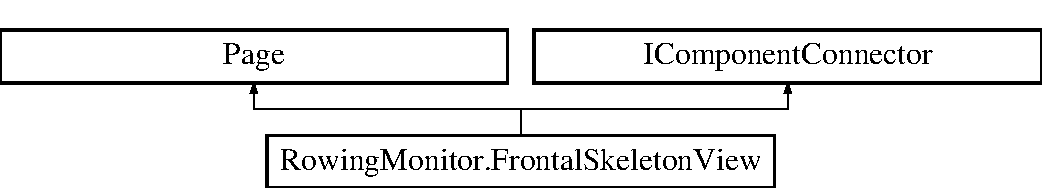
\includegraphics[height=2.000000cm]{class_rowing_monitor_1_1_frontal_skeleton_view}
\end{center}
\end{figure}
\subsection*{Public Member Functions}
\begin{DoxyCompactItemize}
\item 
void \hyperlink{class_rowing_monitor_1_1_frontal_skeleton_view_a201294a5b785283d5d71eeb51a5ad112}{Initialize\+Component} ()
\begin{DoxyCompactList}\small\item\em Initialize\+Component \end{DoxyCompactList}\end{DoxyCompactItemize}


\subsection{Detailed Description}
\hyperlink{class_rowing_monitor_1_1_frontal_skeleton_view}{Frontal\+Skeleton\+View} 



\subsection{Member Function Documentation}
\mbox{\Hypertarget{class_rowing_monitor_1_1_frontal_skeleton_view_a201294a5b785283d5d71eeb51a5ad112}\label{class_rowing_monitor_1_1_frontal_skeleton_view_a201294a5b785283d5d71eeb51a5ad112}} 
\index{Rowing\+Monitor\+::\+Frontal\+Skeleton\+View@{Rowing\+Monitor\+::\+Frontal\+Skeleton\+View}!Initialize\+Component@{Initialize\+Component}}
\index{Initialize\+Component@{Initialize\+Component}!Rowing\+Monitor\+::\+Frontal\+Skeleton\+View@{Rowing\+Monitor\+::\+Frontal\+Skeleton\+View}}
\subsubsection{\texorpdfstring{Initialize\+Component()}{InitializeComponent()}}
{\footnotesize\ttfamily void Rowing\+Monitor.\+Frontal\+Skeleton\+View.\+Initialize\+Component (\begin{DoxyParamCaption}{ }\end{DoxyParamCaption})}



Initialize\+Component 



The documentation for this class was generated from the following file\+:\begin{DoxyCompactItemize}
\item 
obj/\+Debug/\hyperlink{_frontal_skeleton_view_8g_8i_8cs}{Frontal\+Skeleton\+View.\+g.\+i.\+cs}\end{DoxyCompactItemize}

\hypertarget{class_xaml_generated_namespace_1_1_generated_internal_type_helper}{}\section{Xaml\+Generated\+Namespace.\+Generated\+Internal\+Type\+Helper Class Reference}
\label{class_xaml_generated_namespace_1_1_generated_internal_type_helper}\index{Xaml\+Generated\+Namespace.\+Generated\+Internal\+Type\+Helper@{Xaml\+Generated\+Namespace.\+Generated\+Internal\+Type\+Helper}}


\hyperlink{class_xaml_generated_namespace_1_1_generated_internal_type_helper}{Generated\+Internal\+Type\+Helper}  


Inheritance diagram for Xaml\+Generated\+Namespace.\+Generated\+Internal\+Type\+Helper\+:\begin{figure}[H]
\begin{center}
\leavevmode
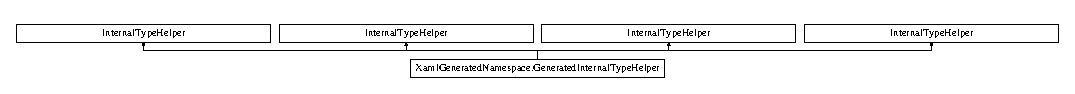
\includegraphics[height=2.000000cm]{class_xaml_generated_namespace_1_1_generated_internal_type_helper}
\end{center}
\end{figure}
\subsection*{Protected Member Functions}
\begin{DoxyCompactItemize}
\item 
override object \hyperlink{class_xaml_generated_namespace_1_1_generated_internal_type_helper_aefb7a98fceb9c287cef4756942f441d1}{Create\+Instance} (System.\+Type type, System.\+Globalization.\+Culture\+Info culture)
\begin{DoxyCompactList}\small\item\em Create\+Instance \end{DoxyCompactList}\item 
override object \hyperlink{class_xaml_generated_namespace_1_1_generated_internal_type_helper_afdc9fe15b56607d02082908d934480c6}{Get\+Property\+Value} (System.\+Reflection.\+Property\+Info property\+Info, object target, System.\+Globalization.\+Culture\+Info culture)
\begin{DoxyCompactList}\small\item\em Get\+Property\+Value \end{DoxyCompactList}\item 
override void \hyperlink{class_xaml_generated_namespace_1_1_generated_internal_type_helper_ade0f04c0f7b18dd5b170e071d5534d38}{Set\+Property\+Value} (System.\+Reflection.\+Property\+Info property\+Info, object target, object value, System.\+Globalization.\+Culture\+Info culture)
\begin{DoxyCompactList}\small\item\em Set\+Property\+Value \end{DoxyCompactList}\item 
override System.\+Delegate \hyperlink{class_xaml_generated_namespace_1_1_generated_internal_type_helper_a8ec4c37e82d9f4e867e9655f4eac3a78}{Create\+Delegate} (System.\+Type delegate\+Type, object target, string handler)
\begin{DoxyCompactList}\small\item\em Create\+Delegate \end{DoxyCompactList}\item 
override void \hyperlink{class_xaml_generated_namespace_1_1_generated_internal_type_helper_a73471f4a6d1ca4c4fceec9ad8610f0c8}{Add\+Event\+Handler} (System.\+Reflection.\+Event\+Info event\+Info, object target, System.\+Delegate handler)
\begin{DoxyCompactList}\small\item\em Add\+Event\+Handler \end{DoxyCompactList}\end{DoxyCompactItemize}


\subsection{Detailed Description}
\hyperlink{class_xaml_generated_namespace_1_1_generated_internal_type_helper}{Generated\+Internal\+Type\+Helper} 



\subsection{Member Function Documentation}
\mbox{\Hypertarget{class_xaml_generated_namespace_1_1_generated_internal_type_helper_a73471f4a6d1ca4c4fceec9ad8610f0c8}\label{class_xaml_generated_namespace_1_1_generated_internal_type_helper_a73471f4a6d1ca4c4fceec9ad8610f0c8}} 
\index{Xaml\+Generated\+Namespace\+::\+Generated\+Internal\+Type\+Helper@{Xaml\+Generated\+Namespace\+::\+Generated\+Internal\+Type\+Helper}!Add\+Event\+Handler@{Add\+Event\+Handler}}
\index{Add\+Event\+Handler@{Add\+Event\+Handler}!Xaml\+Generated\+Namespace\+::\+Generated\+Internal\+Type\+Helper@{Xaml\+Generated\+Namespace\+::\+Generated\+Internal\+Type\+Helper}}
\subsubsection{\texorpdfstring{Add\+Event\+Handler()}{AddEventHandler()}}
{\footnotesize\ttfamily override void Xaml\+Generated\+Namespace.\+Generated\+Internal\+Type\+Helper.\+Add\+Event\+Handler (\begin{DoxyParamCaption}\item[{System.\+Reflection.\+Event\+Info}]{event\+Info,  }\item[{object}]{target,  }\item[{System.\+Delegate}]{handler }\end{DoxyParamCaption})\hspace{0.3cm}{\ttfamily [protected]}}



Add\+Event\+Handler 

\mbox{\Hypertarget{class_xaml_generated_namespace_1_1_generated_internal_type_helper_a8ec4c37e82d9f4e867e9655f4eac3a78}\label{class_xaml_generated_namespace_1_1_generated_internal_type_helper_a8ec4c37e82d9f4e867e9655f4eac3a78}} 
\index{Xaml\+Generated\+Namespace\+::\+Generated\+Internal\+Type\+Helper@{Xaml\+Generated\+Namespace\+::\+Generated\+Internal\+Type\+Helper}!Create\+Delegate@{Create\+Delegate}}
\index{Create\+Delegate@{Create\+Delegate}!Xaml\+Generated\+Namespace\+::\+Generated\+Internal\+Type\+Helper@{Xaml\+Generated\+Namespace\+::\+Generated\+Internal\+Type\+Helper}}
\subsubsection{\texorpdfstring{Create\+Delegate()}{CreateDelegate()}}
{\footnotesize\ttfamily override System.\+Delegate Xaml\+Generated\+Namespace.\+Generated\+Internal\+Type\+Helper.\+Create\+Delegate (\begin{DoxyParamCaption}\item[{System.\+Type}]{delegate\+Type,  }\item[{object}]{target,  }\item[{string}]{handler }\end{DoxyParamCaption})\hspace{0.3cm}{\ttfamily [protected]}}



Create\+Delegate 

\mbox{\Hypertarget{class_xaml_generated_namespace_1_1_generated_internal_type_helper_aefb7a98fceb9c287cef4756942f441d1}\label{class_xaml_generated_namespace_1_1_generated_internal_type_helper_aefb7a98fceb9c287cef4756942f441d1}} 
\index{Xaml\+Generated\+Namespace\+::\+Generated\+Internal\+Type\+Helper@{Xaml\+Generated\+Namespace\+::\+Generated\+Internal\+Type\+Helper}!Create\+Instance@{Create\+Instance}}
\index{Create\+Instance@{Create\+Instance}!Xaml\+Generated\+Namespace\+::\+Generated\+Internal\+Type\+Helper@{Xaml\+Generated\+Namespace\+::\+Generated\+Internal\+Type\+Helper}}
\subsubsection{\texorpdfstring{Create\+Instance()}{CreateInstance()}}
{\footnotesize\ttfamily override object Xaml\+Generated\+Namespace.\+Generated\+Internal\+Type\+Helper.\+Create\+Instance (\begin{DoxyParamCaption}\item[{System.\+Type}]{type,  }\item[{System.\+Globalization.\+Culture\+Info}]{culture }\end{DoxyParamCaption})\hspace{0.3cm}{\ttfamily [protected]}}



Create\+Instance 

\mbox{\Hypertarget{class_xaml_generated_namespace_1_1_generated_internal_type_helper_afdc9fe15b56607d02082908d934480c6}\label{class_xaml_generated_namespace_1_1_generated_internal_type_helper_afdc9fe15b56607d02082908d934480c6}} 
\index{Xaml\+Generated\+Namespace\+::\+Generated\+Internal\+Type\+Helper@{Xaml\+Generated\+Namespace\+::\+Generated\+Internal\+Type\+Helper}!Get\+Property\+Value@{Get\+Property\+Value}}
\index{Get\+Property\+Value@{Get\+Property\+Value}!Xaml\+Generated\+Namespace\+::\+Generated\+Internal\+Type\+Helper@{Xaml\+Generated\+Namespace\+::\+Generated\+Internal\+Type\+Helper}}
\subsubsection{\texorpdfstring{Get\+Property\+Value()}{GetPropertyValue()}}
{\footnotesize\ttfamily override object Xaml\+Generated\+Namespace.\+Generated\+Internal\+Type\+Helper.\+Get\+Property\+Value (\begin{DoxyParamCaption}\item[{System.\+Reflection.\+Property\+Info}]{property\+Info,  }\item[{object}]{target,  }\item[{System.\+Globalization.\+Culture\+Info}]{culture }\end{DoxyParamCaption})\hspace{0.3cm}{\ttfamily [protected]}}



Get\+Property\+Value 

\mbox{\Hypertarget{class_xaml_generated_namespace_1_1_generated_internal_type_helper_ade0f04c0f7b18dd5b170e071d5534d38}\label{class_xaml_generated_namespace_1_1_generated_internal_type_helper_ade0f04c0f7b18dd5b170e071d5534d38}} 
\index{Xaml\+Generated\+Namespace\+::\+Generated\+Internal\+Type\+Helper@{Xaml\+Generated\+Namespace\+::\+Generated\+Internal\+Type\+Helper}!Set\+Property\+Value@{Set\+Property\+Value}}
\index{Set\+Property\+Value@{Set\+Property\+Value}!Xaml\+Generated\+Namespace\+::\+Generated\+Internal\+Type\+Helper@{Xaml\+Generated\+Namespace\+::\+Generated\+Internal\+Type\+Helper}}
\subsubsection{\texorpdfstring{Set\+Property\+Value()}{SetPropertyValue()}}
{\footnotesize\ttfamily override void Xaml\+Generated\+Namespace.\+Generated\+Internal\+Type\+Helper.\+Set\+Property\+Value (\begin{DoxyParamCaption}\item[{System.\+Reflection.\+Property\+Info}]{property\+Info,  }\item[{object}]{target,  }\item[{object}]{value,  }\item[{System.\+Globalization.\+Culture\+Info}]{culture }\end{DoxyParamCaption})\hspace{0.3cm}{\ttfamily [protected]}}



Set\+Property\+Value 



The documentation for this class was generated from the following file\+:\begin{DoxyCompactItemize}
\item 
obj/\+Debug/\hyperlink{_generated_internal_type_helper_8g_8i_8cs}{Generated\+Internal\+Type\+Helper.\+g.\+i.\+cs}\end{DoxyCompactItemize}

\hypertarget{class_rowing_monitor_1_1_view_1_1_home_view}{}\section{Rowing\+Monitor.\+View.\+Home\+View Class Reference}
\label{class_rowing_monitor_1_1_view_1_1_home_view}\index{Rowing\+Monitor.\+View.\+Home\+View@{Rowing\+Monitor.\+View.\+Home\+View}}


\hyperlink{class_rowing_monitor_1_1_view_1_1_home_view}{Home\+View}  


Inheritance diagram for Rowing\+Monitor.\+View.\+Home\+View\+:\begin{figure}[H]
\begin{center}
\leavevmode
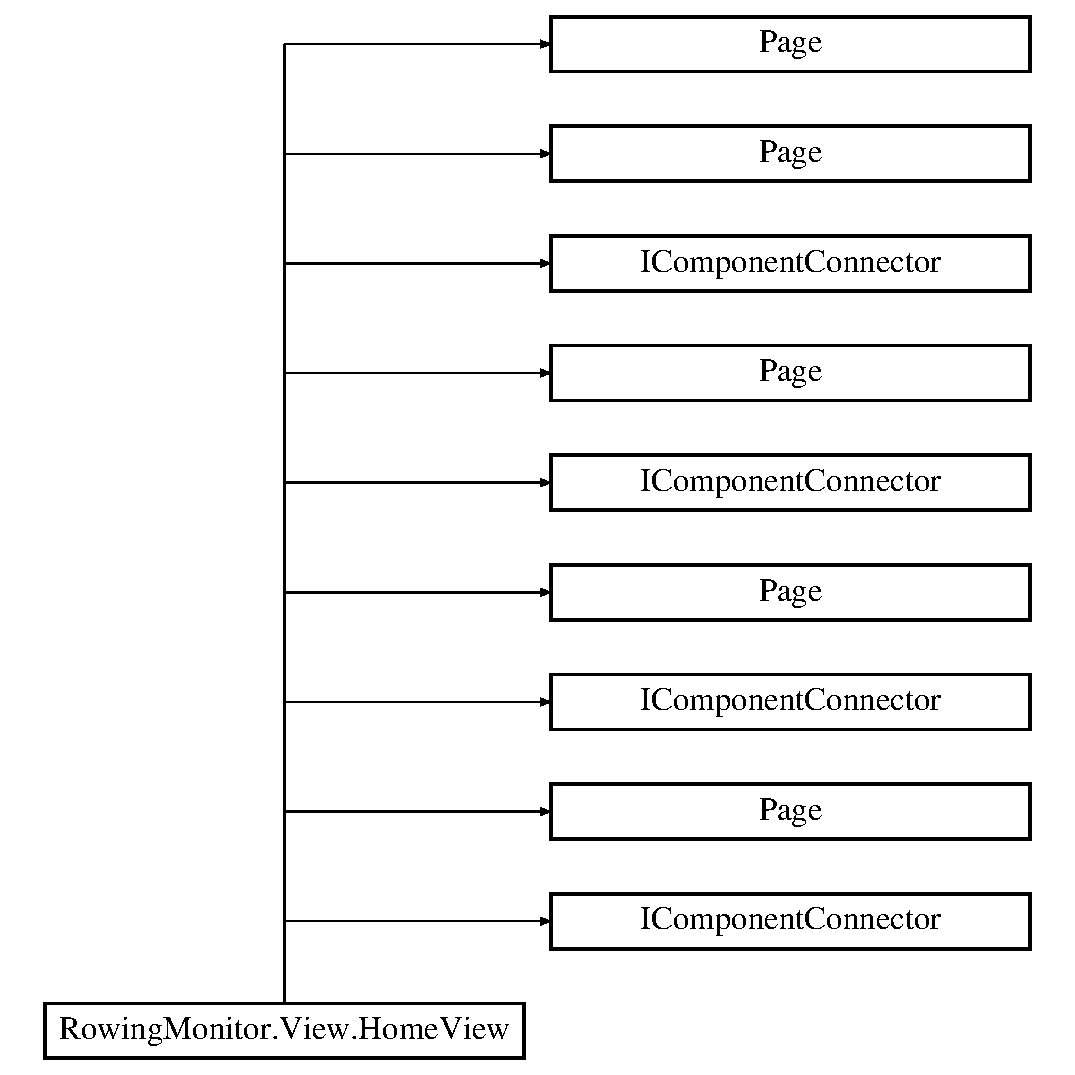
\includegraphics[height=10.000000cm]{class_rowing_monitor_1_1_view_1_1_home_view}
\end{center}
\end{figure}
\subsection*{Public Member Functions}
\begin{DoxyCompactItemize}
\item 
void \hyperlink{class_rowing_monitor_1_1_view_1_1_home_view_af517b7b90bd5fd7c31122f3058e32d4c}{Initialize\+Component} ()
\begin{DoxyCompactList}\small\item\em Initialize\+Component \end{DoxyCompactList}\item 
void \hyperlink{class_rowing_monitor_1_1_view_1_1_home_view_af517b7b90bd5fd7c31122f3058e32d4c}{Initialize\+Component} ()
\begin{DoxyCompactList}\small\item\em Initialize\+Component \end{DoxyCompactList}\item 
void \hyperlink{class_rowing_monitor_1_1_view_1_1_home_view_af517b7b90bd5fd7c31122f3058e32d4c}{Initialize\+Component} ()
\begin{DoxyCompactList}\small\item\em Initialize\+Component \end{DoxyCompactList}\item 
void \hyperlink{class_rowing_monitor_1_1_view_1_1_home_view_af517b7b90bd5fd7c31122f3058e32d4c}{Initialize\+Component} ()
\begin{DoxyCompactList}\small\item\em Initialize\+Component \end{DoxyCompactList}\item 
\hyperlink{class_rowing_monitor_1_1_view_1_1_home_view_a8b4e20793bd293f4e821c78b7f1d1281}{Home\+View} ()
\end{DoxyCompactItemize}


\subsection{Detailed Description}
\hyperlink{class_rowing_monitor_1_1_view_1_1_home_view}{Home\+View} 

Interaktionslogik für Home\+View.\+xaml 

\subsection{Constructor \& Destructor Documentation}
\mbox{\Hypertarget{class_rowing_monitor_1_1_view_1_1_home_view_a8b4e20793bd293f4e821c78b7f1d1281}\label{class_rowing_monitor_1_1_view_1_1_home_view_a8b4e20793bd293f4e821c78b7f1d1281}} 
\index{Rowing\+Monitor\+::\+View\+::\+Home\+View@{Rowing\+Monitor\+::\+View\+::\+Home\+View}!Home\+View@{Home\+View}}
\index{Home\+View@{Home\+View}!Rowing\+Monitor\+::\+View\+::\+Home\+View@{Rowing\+Monitor\+::\+View\+::\+Home\+View}}
\subsubsection{\texorpdfstring{Home\+View()}{HomeView()}}
{\footnotesize\ttfamily Rowing\+Monitor.\+View.\+Home\+View.\+Home\+View (\begin{DoxyParamCaption}{ }\end{DoxyParamCaption})}



\subsection{Member Function Documentation}
\mbox{\Hypertarget{class_rowing_monitor_1_1_view_1_1_home_view_af517b7b90bd5fd7c31122f3058e32d4c}\label{class_rowing_monitor_1_1_view_1_1_home_view_af517b7b90bd5fd7c31122f3058e32d4c}} 
\index{Rowing\+Monitor\+::\+View\+::\+Home\+View@{Rowing\+Monitor\+::\+View\+::\+Home\+View}!Initialize\+Component@{Initialize\+Component}}
\index{Initialize\+Component@{Initialize\+Component}!Rowing\+Monitor\+::\+View\+::\+Home\+View@{Rowing\+Monitor\+::\+View\+::\+Home\+View}}
\subsubsection{\texorpdfstring{Initialize\+Component()}{InitializeComponent()}\hspace{0.1cm}{\footnotesize\ttfamily [1/4]}}
{\footnotesize\ttfamily void Rowing\+Monitor.\+View.\+Home\+View.\+Initialize\+Component (\begin{DoxyParamCaption}{ }\end{DoxyParamCaption})}



Initialize\+Component 

\mbox{\Hypertarget{class_rowing_monitor_1_1_view_1_1_home_view_af517b7b90bd5fd7c31122f3058e32d4c}\label{class_rowing_monitor_1_1_view_1_1_home_view_af517b7b90bd5fd7c31122f3058e32d4c}} 
\index{Rowing\+Monitor\+::\+View\+::\+Home\+View@{Rowing\+Monitor\+::\+View\+::\+Home\+View}!Initialize\+Component@{Initialize\+Component}}
\index{Initialize\+Component@{Initialize\+Component}!Rowing\+Monitor\+::\+View\+::\+Home\+View@{Rowing\+Monitor\+::\+View\+::\+Home\+View}}
\subsubsection{\texorpdfstring{Initialize\+Component()}{InitializeComponent()}\hspace{0.1cm}{\footnotesize\ttfamily [2/4]}}
{\footnotesize\ttfamily void Rowing\+Monitor.\+View.\+Home\+View.\+Initialize\+Component (\begin{DoxyParamCaption}{ }\end{DoxyParamCaption})}



Initialize\+Component 

\mbox{\Hypertarget{class_rowing_monitor_1_1_view_1_1_home_view_af517b7b90bd5fd7c31122f3058e32d4c}\label{class_rowing_monitor_1_1_view_1_1_home_view_af517b7b90bd5fd7c31122f3058e32d4c}} 
\index{Rowing\+Monitor\+::\+View\+::\+Home\+View@{Rowing\+Monitor\+::\+View\+::\+Home\+View}!Initialize\+Component@{Initialize\+Component}}
\index{Initialize\+Component@{Initialize\+Component}!Rowing\+Monitor\+::\+View\+::\+Home\+View@{Rowing\+Monitor\+::\+View\+::\+Home\+View}}
\subsubsection{\texorpdfstring{Initialize\+Component()}{InitializeComponent()}\hspace{0.1cm}{\footnotesize\ttfamily [3/4]}}
{\footnotesize\ttfamily void Rowing\+Monitor.\+View.\+Home\+View.\+Initialize\+Component (\begin{DoxyParamCaption}{ }\end{DoxyParamCaption})}



Initialize\+Component 

\mbox{\Hypertarget{class_rowing_monitor_1_1_view_1_1_home_view_af517b7b90bd5fd7c31122f3058e32d4c}\label{class_rowing_monitor_1_1_view_1_1_home_view_af517b7b90bd5fd7c31122f3058e32d4c}} 
\index{Rowing\+Monitor\+::\+View\+::\+Home\+View@{Rowing\+Monitor\+::\+View\+::\+Home\+View}!Initialize\+Component@{Initialize\+Component}}
\index{Initialize\+Component@{Initialize\+Component}!Rowing\+Monitor\+::\+View\+::\+Home\+View@{Rowing\+Monitor\+::\+View\+::\+Home\+View}}
\subsubsection{\texorpdfstring{Initialize\+Component()}{InitializeComponent()}\hspace{0.1cm}{\footnotesize\ttfamily [4/4]}}
{\footnotesize\ttfamily void Rowing\+Monitor.\+View.\+Home\+View.\+Initialize\+Component (\begin{DoxyParamCaption}{ }\end{DoxyParamCaption})}



Initialize\+Component 



The documentation for this class was generated from the following files\+:\begin{DoxyCompactItemize}
\item 
obj/\+Debug/\+View/\hyperlink{_debug_2_view_2_home_view_8g_8cs}{Home\+View.\+g.\+cs}\item 
obj/\+Debug/\+View/\hyperlink{_debug_2_view_2_home_view_8g_8i_8cs}{Home\+View.\+g.\+i.\+cs}\item 
View/\hyperlink{_home_view_8xaml_8cs}{Home\+View.\+xaml.\+cs}\end{DoxyCompactItemize}

\hypertarget{class_rowing_monitor_1_1_view_model_1_1_home_view_model}{}\section{Rowing\+Monitor.\+View\+Model.\+Home\+View\+Model Class Reference}
\label{class_rowing_monitor_1_1_view_model_1_1_home_view_model}\index{Rowing\+Monitor.\+View\+Model.\+Home\+View\+Model@{Rowing\+Monitor.\+View\+Model.\+Home\+View\+Model}}
\subsection*{Public Member Functions}
\begin{DoxyCompactItemize}
\item 
\hyperlink{class_rowing_monitor_1_1_view_model_1_1_home_view_model_a6aeb83011dc7837b14abb2dac7e56aaa}{Home\+View\+Model} ()
\item 
void \hyperlink{class_rowing_monitor_1_1_view_model_1_1_home_view_model_ab20700b532293270bc43551ddcc783c6}{View\+Loaded} ()
\item 
void \hyperlink{class_rowing_monitor_1_1_view_model_1_1_home_view_model_adea01e64945f13fb6beafb3804b8fd6d}{View\+Unloaded} ()
\end{DoxyCompactItemize}
\subsection*{Properties}
\begin{DoxyCompactItemize}
\item 
Grid \hyperlink{class_rowing_monitor_1_1_view_model_1_1_home_view_model_a6a13d06451d7375e39108c273022cef4}{G\+U\+I\+Grid}\hspace{0.3cm}{\ttfamily  \mbox{[}get, set\mbox{]}}
\end{DoxyCompactItemize}


\subsection{Constructor \& Destructor Documentation}
\mbox{\Hypertarget{class_rowing_monitor_1_1_view_model_1_1_home_view_model_a6aeb83011dc7837b14abb2dac7e56aaa}\label{class_rowing_monitor_1_1_view_model_1_1_home_view_model_a6aeb83011dc7837b14abb2dac7e56aaa}} 
\index{Rowing\+Monitor\+::\+View\+Model\+::\+Home\+View\+Model@{Rowing\+Monitor\+::\+View\+Model\+::\+Home\+View\+Model}!Home\+View\+Model@{Home\+View\+Model}}
\index{Home\+View\+Model@{Home\+View\+Model}!Rowing\+Monitor\+::\+View\+Model\+::\+Home\+View\+Model@{Rowing\+Monitor\+::\+View\+Model\+::\+Home\+View\+Model}}
\subsubsection{\texorpdfstring{Home\+View\+Model()}{HomeViewModel()}}
{\footnotesize\ttfamily Rowing\+Monitor.\+View\+Model.\+Home\+View\+Model.\+Home\+View\+Model (\begin{DoxyParamCaption}{ }\end{DoxyParamCaption})}



\subsection{Member Function Documentation}
\mbox{\Hypertarget{class_rowing_monitor_1_1_view_model_1_1_home_view_model_ab20700b532293270bc43551ddcc783c6}\label{class_rowing_monitor_1_1_view_model_1_1_home_view_model_ab20700b532293270bc43551ddcc783c6}} 
\index{Rowing\+Monitor\+::\+View\+Model\+::\+Home\+View\+Model@{Rowing\+Monitor\+::\+View\+Model\+::\+Home\+View\+Model}!View\+Loaded@{View\+Loaded}}
\index{View\+Loaded@{View\+Loaded}!Rowing\+Monitor\+::\+View\+Model\+::\+Home\+View\+Model@{Rowing\+Monitor\+::\+View\+Model\+::\+Home\+View\+Model}}
\subsubsection{\texorpdfstring{View\+Loaded()}{ViewLoaded()}}
{\footnotesize\ttfamily void Rowing\+Monitor.\+View\+Model.\+Home\+View\+Model.\+View\+Loaded (\begin{DoxyParamCaption}{ }\end{DoxyParamCaption})}

\mbox{\Hypertarget{class_rowing_monitor_1_1_view_model_1_1_home_view_model_adea01e64945f13fb6beafb3804b8fd6d}\label{class_rowing_monitor_1_1_view_model_1_1_home_view_model_adea01e64945f13fb6beafb3804b8fd6d}} 
\index{Rowing\+Monitor\+::\+View\+Model\+::\+Home\+View\+Model@{Rowing\+Monitor\+::\+View\+Model\+::\+Home\+View\+Model}!View\+Unloaded@{View\+Unloaded}}
\index{View\+Unloaded@{View\+Unloaded}!Rowing\+Monitor\+::\+View\+Model\+::\+Home\+View\+Model@{Rowing\+Monitor\+::\+View\+Model\+::\+Home\+View\+Model}}
\subsubsection{\texorpdfstring{View\+Unloaded()}{ViewUnloaded()}}
{\footnotesize\ttfamily void Rowing\+Monitor.\+View\+Model.\+Home\+View\+Model.\+View\+Unloaded (\begin{DoxyParamCaption}{ }\end{DoxyParamCaption})}



\subsection{Property Documentation}
\mbox{\Hypertarget{class_rowing_monitor_1_1_view_model_1_1_home_view_model_a6a13d06451d7375e39108c273022cef4}\label{class_rowing_monitor_1_1_view_model_1_1_home_view_model_a6a13d06451d7375e39108c273022cef4}} 
\index{Rowing\+Monitor\+::\+View\+Model\+::\+Home\+View\+Model@{Rowing\+Monitor\+::\+View\+Model\+::\+Home\+View\+Model}!G\+U\+I\+Grid@{G\+U\+I\+Grid}}
\index{G\+U\+I\+Grid@{G\+U\+I\+Grid}!Rowing\+Monitor\+::\+View\+Model\+::\+Home\+View\+Model@{Rowing\+Monitor\+::\+View\+Model\+::\+Home\+View\+Model}}
\subsubsection{\texorpdfstring{G\+U\+I\+Grid}{GUIGrid}}
{\footnotesize\ttfamily Grid Rowing\+Monitor.\+View\+Model.\+Home\+View\+Model.\+G\+U\+I\+Grid\hspace{0.3cm}{\ttfamily [get]}, {\ttfamily [set]}}



The documentation for this class was generated from the following file\+:\begin{DoxyCompactItemize}
\item 
View\+Model/\hyperlink{_home_view_model_8cs}{Home\+View\+Model.\+cs}\end{DoxyCompactItemize}

\hypertarget{struct_rowing_monitor_1_1_model_1_1_util_1_1_joint_data}{}\section{Rowing\+Monitor.\+Model.\+Util.\+Joint\+Data Struct Reference}
\label{struct_rowing_monitor_1_1_model_1_1_util_1_1_joint_data}\index{Rowing\+Monitor.\+Model.\+Util.\+Joint\+Data@{Rowing\+Monitor.\+Model.\+Util.\+Joint\+Data}}
\subsection*{Properties}
\begin{DoxyCompactItemize}
\item 
double \hyperlink{struct_rowing_monitor_1_1_model_1_1_util_1_1_joint_data_a56463d7bd16c6e5cad4e3619e9df9508}{Rel\+Timestamp}\hspace{0.3cm}{\ttfamily  \mbox{[}get, set\mbox{]}}
\begin{DoxyCompactList}\small\item\em Time in milliseconds since Kinect sensor started. \end{DoxyCompactList}\item 
double \hyperlink{struct_rowing_monitor_1_1_model_1_1_util_1_1_joint_data_a2c951ee40b3e49be73b92cf39c5aa9ab}{Abs\+Timestamp}\hspace{0.3cm}{\ttfamily  \mbox{[}get, set\mbox{]}}
\begin{DoxyCompactList}\small\item\em Time in milliseconds since first frame. \end{DoxyCompactList}\item 
I\+Read\+Only\+Dictionary$<$ Joint\+Type, Joint $>$ \hyperlink{struct_rowing_monitor_1_1_model_1_1_util_1_1_joint_data_afa67f920730db9679102686913774e69}{Joints}\hspace{0.3cm}{\ttfamily  \mbox{[}get, set\mbox{]}}
\begin{DoxyCompactList}\small\item\em Positions of all joints. \end{DoxyCompactList}\item 
long \hyperlink{struct_rowing_monitor_1_1_model_1_1_util_1_1_joint_data_a2193c6359b3e9e2d6dfdb6178351a8b3}{Index}\hspace{0.3cm}{\ttfamily  \mbox{[}get, set\mbox{]}}
\begin{DoxyCompactList}\small\item\em Incrementing number of frames. \end{DoxyCompactList}\item 
List$<$ double $>$ \hyperlink{struct_rowing_monitor_1_1_model_1_1_util_1_1_joint_data_a98bf571ea92c7f9b8e197062f17ddc27}{Timestamps}\hspace{0.3cm}{\ttfamily  \mbox{[}get, set\mbox{]}}
\begin{DoxyCompactList}\small\item\em List of all timestamps that were set in the pipeline \end{DoxyCompactList}\item 
\hyperlink{namespace_rowing_monitor_1_1_model_1_1_util_a01e1a06061533b246feb7421c9d0107f}{Data\+Stream\+Type} \hyperlink{struct_rowing_monitor_1_1_model_1_1_util_1_1_joint_data_a8ed0022c598484f0b418ad30b50bbfb6}{Data\+Stream\+Type}\hspace{0.3cm}{\ttfamily  \mbox{[}get, set\mbox{]}}
\begin{DoxyCompactList}\small\item\em Type of the data. \end{DoxyCompactList}\item 
bool \hyperlink{struct_rowing_monitor_1_1_model_1_1_util_1_1_joint_data_a1e86bf9206df62d0fb4b77c8017ccf8a}{Is\+Empty}\hspace{0.3cm}{\ttfamily  \mbox{[}get\mbox{]}}
\begin{DoxyCompactList}\small\item\em Returns true if this element conatins no joint data. \end{DoxyCompactList}\end{DoxyCompactItemize}


\subsection{Property Documentation}
\mbox{\Hypertarget{struct_rowing_monitor_1_1_model_1_1_util_1_1_joint_data_a2c951ee40b3e49be73b92cf39c5aa9ab}\label{struct_rowing_monitor_1_1_model_1_1_util_1_1_joint_data_a2c951ee40b3e49be73b92cf39c5aa9ab}} 
\index{Rowing\+Monitor\+::\+Model\+::\+Util\+::\+Joint\+Data@{Rowing\+Monitor\+::\+Model\+::\+Util\+::\+Joint\+Data}!Abs\+Timestamp@{Abs\+Timestamp}}
\index{Abs\+Timestamp@{Abs\+Timestamp}!Rowing\+Monitor\+::\+Model\+::\+Util\+::\+Joint\+Data@{Rowing\+Monitor\+::\+Model\+::\+Util\+::\+Joint\+Data}}
\subsubsection{\texorpdfstring{Abs\+Timestamp}{AbsTimestamp}}
{\footnotesize\ttfamily double Rowing\+Monitor.\+Model.\+Util.\+Joint\+Data.\+Abs\+Timestamp\hspace{0.3cm}{\ttfamily [get]}, {\ttfamily [set]}}



Time in milliseconds since first frame. 

\mbox{\Hypertarget{struct_rowing_monitor_1_1_model_1_1_util_1_1_joint_data_a8ed0022c598484f0b418ad30b50bbfb6}\label{struct_rowing_monitor_1_1_model_1_1_util_1_1_joint_data_a8ed0022c598484f0b418ad30b50bbfb6}} 
\index{Rowing\+Monitor\+::\+Model\+::\+Util\+::\+Joint\+Data@{Rowing\+Monitor\+::\+Model\+::\+Util\+::\+Joint\+Data}!Data\+Stream\+Type@{Data\+Stream\+Type}}
\index{Data\+Stream\+Type@{Data\+Stream\+Type}!Rowing\+Monitor\+::\+Model\+::\+Util\+::\+Joint\+Data@{Rowing\+Monitor\+::\+Model\+::\+Util\+::\+Joint\+Data}}
\subsubsection{\texorpdfstring{Data\+Stream\+Type}{DataStreamType}}
{\footnotesize\ttfamily \hyperlink{namespace_rowing_monitor_1_1_model_1_1_util_a01e1a06061533b246feb7421c9d0107f}{Data\+Stream\+Type} Rowing\+Monitor.\+Model.\+Util.\+Joint\+Data.\+Data\+Stream\+Type\hspace{0.3cm}{\ttfamily [get]}, {\ttfamily [set]}}



Type of the data. 

\mbox{\Hypertarget{struct_rowing_monitor_1_1_model_1_1_util_1_1_joint_data_a2193c6359b3e9e2d6dfdb6178351a8b3}\label{struct_rowing_monitor_1_1_model_1_1_util_1_1_joint_data_a2193c6359b3e9e2d6dfdb6178351a8b3}} 
\index{Rowing\+Monitor\+::\+Model\+::\+Util\+::\+Joint\+Data@{Rowing\+Monitor\+::\+Model\+::\+Util\+::\+Joint\+Data}!Index@{Index}}
\index{Index@{Index}!Rowing\+Monitor\+::\+Model\+::\+Util\+::\+Joint\+Data@{Rowing\+Monitor\+::\+Model\+::\+Util\+::\+Joint\+Data}}
\subsubsection{\texorpdfstring{Index}{Index}}
{\footnotesize\ttfamily long Rowing\+Monitor.\+Model.\+Util.\+Joint\+Data.\+Index\hspace{0.3cm}{\ttfamily [get]}, {\ttfamily [set]}}



Incrementing number of frames. 

\mbox{\Hypertarget{struct_rowing_monitor_1_1_model_1_1_util_1_1_joint_data_a1e86bf9206df62d0fb4b77c8017ccf8a}\label{struct_rowing_monitor_1_1_model_1_1_util_1_1_joint_data_a1e86bf9206df62d0fb4b77c8017ccf8a}} 
\index{Rowing\+Monitor\+::\+Model\+::\+Util\+::\+Joint\+Data@{Rowing\+Monitor\+::\+Model\+::\+Util\+::\+Joint\+Data}!Is\+Empty@{Is\+Empty}}
\index{Is\+Empty@{Is\+Empty}!Rowing\+Monitor\+::\+Model\+::\+Util\+::\+Joint\+Data@{Rowing\+Monitor\+::\+Model\+::\+Util\+::\+Joint\+Data}}
\subsubsection{\texorpdfstring{Is\+Empty}{IsEmpty}}
{\footnotesize\ttfamily bool Rowing\+Monitor.\+Model.\+Util.\+Joint\+Data.\+Is\+Empty\hspace{0.3cm}{\ttfamily [get]}}



Returns true if this element conatins no joint data. 

\mbox{\Hypertarget{struct_rowing_monitor_1_1_model_1_1_util_1_1_joint_data_afa67f920730db9679102686913774e69}\label{struct_rowing_monitor_1_1_model_1_1_util_1_1_joint_data_afa67f920730db9679102686913774e69}} 
\index{Rowing\+Monitor\+::\+Model\+::\+Util\+::\+Joint\+Data@{Rowing\+Monitor\+::\+Model\+::\+Util\+::\+Joint\+Data}!Joints@{Joints}}
\index{Joints@{Joints}!Rowing\+Monitor\+::\+Model\+::\+Util\+::\+Joint\+Data@{Rowing\+Monitor\+::\+Model\+::\+Util\+::\+Joint\+Data}}
\subsubsection{\texorpdfstring{Joints}{Joints}}
{\footnotesize\ttfamily I\+Read\+Only\+Dictionary$<$Joint\+Type, Joint$>$ Rowing\+Monitor.\+Model.\+Util.\+Joint\+Data.\+Joints\hspace{0.3cm}{\ttfamily [get]}, {\ttfamily [set]}}



Positions of all joints. 

\mbox{\Hypertarget{struct_rowing_monitor_1_1_model_1_1_util_1_1_joint_data_a56463d7bd16c6e5cad4e3619e9df9508}\label{struct_rowing_monitor_1_1_model_1_1_util_1_1_joint_data_a56463d7bd16c6e5cad4e3619e9df9508}} 
\index{Rowing\+Monitor\+::\+Model\+::\+Util\+::\+Joint\+Data@{Rowing\+Monitor\+::\+Model\+::\+Util\+::\+Joint\+Data}!Rel\+Timestamp@{Rel\+Timestamp}}
\index{Rel\+Timestamp@{Rel\+Timestamp}!Rowing\+Monitor\+::\+Model\+::\+Util\+::\+Joint\+Data@{Rowing\+Monitor\+::\+Model\+::\+Util\+::\+Joint\+Data}}
\subsubsection{\texorpdfstring{Rel\+Timestamp}{RelTimestamp}}
{\footnotesize\ttfamily double Rowing\+Monitor.\+Model.\+Util.\+Joint\+Data.\+Rel\+Timestamp\hspace{0.3cm}{\ttfamily [get]}, {\ttfamily [set]}}



Time in milliseconds since Kinect sensor started. 

\mbox{\Hypertarget{struct_rowing_monitor_1_1_model_1_1_util_1_1_joint_data_a98bf571ea92c7f9b8e197062f17ddc27}\label{struct_rowing_monitor_1_1_model_1_1_util_1_1_joint_data_a98bf571ea92c7f9b8e197062f17ddc27}} 
\index{Rowing\+Monitor\+::\+Model\+::\+Util\+::\+Joint\+Data@{Rowing\+Monitor\+::\+Model\+::\+Util\+::\+Joint\+Data}!Timestamps@{Timestamps}}
\index{Timestamps@{Timestamps}!Rowing\+Monitor\+::\+Model\+::\+Util\+::\+Joint\+Data@{Rowing\+Monitor\+::\+Model\+::\+Util\+::\+Joint\+Data}}
\subsubsection{\texorpdfstring{Timestamps}{Timestamps}}
{\footnotesize\ttfamily List$<$double$>$ Rowing\+Monitor.\+Model.\+Util.\+Joint\+Data.\+Timestamps\hspace{0.3cm}{\ttfamily [get]}, {\ttfamily [set]}}



List of all timestamps that were set in the pipeline 



The documentation for this struct was generated from the following file\+:\begin{DoxyCompactItemize}
\item 
Model/\+Util/\hyperlink{_joint_data_handler_8cs}{Joint\+Data\+Handler.\+cs}\end{DoxyCompactItemize}

\hypertarget{class_rowing_monitor_1_1_model_1_1_util_1_1_joint_data_handler}{}\section{Rowing\+Monitor.\+Model.\+Util.\+Joint\+Data\+Handler Class Reference}
\label{class_rowing_monitor_1_1_model_1_1_util_1_1_joint_data_handler}\index{Rowing\+Monitor.\+Model.\+Util.\+Joint\+Data\+Handler@{Rowing\+Monitor.\+Model.\+Util.\+Joint\+Data\+Handler}}
\subsection*{Public Member Functions}
\begin{DoxyCompactItemize}
\item 
\hyperlink{struct_rowing_monitor_1_1_model_1_1_util_1_1_joint_data}{Joint\+Data} \hyperlink{class_rowing_monitor_1_1_model_1_1_util_1_1_joint_data_handler_af9945324e3ca88ac94ccc052f172f68d}{Create\+New\+Joint\+Data} (double rel\+Timestamp, double creation\+Timestamp, I\+Read\+Only\+Dictionary$<$ Joint\+Type, Joint $>$ joints)
\item 
Body \hyperlink{class_rowing_monitor_1_1_model_1_1_util_1_1_joint_data_handler_a93577e6689cfac35636d2a97f9ddee49}{Get\+First\+Tracked\+Body} ()
\begin{DoxyCompactList}\small\item\em Return the longest tracked body. \end{DoxyCompactList}\end{DoxyCompactItemize}
\subsection*{Static Public Member Functions}
\begin{DoxyCompactItemize}
\item 
static \hyperlink{struct_rowing_monitor_1_1_model_1_1_util_1_1_joint_data}{Joint\+Data} \hyperlink{class_rowing_monitor_1_1_model_1_1_util_1_1_joint_data_handler_a7fed5b351470a66f22bb242dee429b99}{Replace\+Joints\+In\+Joint\+Data} (\hyperlink{struct_rowing_monitor_1_1_model_1_1_util_1_1_joint_data}{Joint\+Data} old\+Joint\+Data, double creation\+Timestamp, I\+Read\+Only\+Dictionary$<$ Joint\+Type, Joint $>$ new\+Joints, \hyperlink{namespace_rowing_monitor_1_1_model_1_1_util_a01e1a06061533b246feb7421c9d0107f}{Data\+Stream\+Type} data\+Stream\+Type)
\end{DoxyCompactItemize}
\subsection*{Properties}
\begin{DoxyCompactItemize}
\item 
static \hyperlink{class_rowing_monitor_1_1_model_1_1_util_1_1_joint_data_handler}{Joint\+Data\+Handler} \hyperlink{class_rowing_monitor_1_1_model_1_1_util_1_1_joint_data_handler_a3ad8535ad9430e2a635071976a73c2ea}{Instance}\hspace{0.3cm}{\ttfamily  \mbox{[}get\mbox{]}}
\item 
double \hyperlink{class_rowing_monitor_1_1_model_1_1_util_1_1_joint_data_handler_a6a861fd29d1f7d9e5257d2b4fd995e7d}{Rel\+Start\+Time}\hspace{0.3cm}{\ttfamily  \mbox{[}get, set\mbox{]}}
\item 
long \hyperlink{class_rowing_monitor_1_1_model_1_1_util_1_1_joint_data_handler_ae5d278181fb0c1896766b4482e5a4f7e}{Last\+Index}\hspace{0.3cm}{\ttfamily  \mbox{[}get, set\mbox{]}}
\item 
Body \mbox{[}$\,$\mbox{]} \hyperlink{class_rowing_monitor_1_1_model_1_1_util_1_1_joint_data_handler_a0c4ffc4145ad48004d1ffb064801adae}{Bodies}\hspace{0.3cm}{\ttfamily  \mbox{[}get, set\mbox{]}}
\end{DoxyCompactItemize}


\subsection{Member Function Documentation}
\mbox{\Hypertarget{class_rowing_monitor_1_1_model_1_1_util_1_1_joint_data_handler_af9945324e3ca88ac94ccc052f172f68d}\label{class_rowing_monitor_1_1_model_1_1_util_1_1_joint_data_handler_af9945324e3ca88ac94ccc052f172f68d}} 
\index{Rowing\+Monitor\+::\+Model\+::\+Util\+::\+Joint\+Data\+Handler@{Rowing\+Monitor\+::\+Model\+::\+Util\+::\+Joint\+Data\+Handler}!Create\+New\+Joint\+Data@{Create\+New\+Joint\+Data}}
\index{Create\+New\+Joint\+Data@{Create\+New\+Joint\+Data}!Rowing\+Monitor\+::\+Model\+::\+Util\+::\+Joint\+Data\+Handler@{Rowing\+Monitor\+::\+Model\+::\+Util\+::\+Joint\+Data\+Handler}}
\subsubsection{\texorpdfstring{Create\+New\+Joint\+Data()}{CreateNewJointData()}}
{\footnotesize\ttfamily \hyperlink{struct_rowing_monitor_1_1_model_1_1_util_1_1_joint_data}{Joint\+Data} Rowing\+Monitor.\+Model.\+Util.\+Joint\+Data\+Handler.\+Create\+New\+Joint\+Data (\begin{DoxyParamCaption}\item[{double}]{rel\+Timestamp,  }\item[{double}]{creation\+Timestamp,  }\item[{I\+Read\+Only\+Dictionary$<$ Joint\+Type, Joint $>$}]{joints }\end{DoxyParamCaption})}

\mbox{\Hypertarget{class_rowing_monitor_1_1_model_1_1_util_1_1_joint_data_handler_a93577e6689cfac35636d2a97f9ddee49}\label{class_rowing_monitor_1_1_model_1_1_util_1_1_joint_data_handler_a93577e6689cfac35636d2a97f9ddee49}} 
\index{Rowing\+Monitor\+::\+Model\+::\+Util\+::\+Joint\+Data\+Handler@{Rowing\+Monitor\+::\+Model\+::\+Util\+::\+Joint\+Data\+Handler}!Get\+First\+Tracked\+Body@{Get\+First\+Tracked\+Body}}
\index{Get\+First\+Tracked\+Body@{Get\+First\+Tracked\+Body}!Rowing\+Monitor\+::\+Model\+::\+Util\+::\+Joint\+Data\+Handler@{Rowing\+Monitor\+::\+Model\+::\+Util\+::\+Joint\+Data\+Handler}}
\subsubsection{\texorpdfstring{Get\+First\+Tracked\+Body()}{GetFirstTrackedBody()}}
{\footnotesize\ttfamily Body Rowing\+Monitor.\+Model.\+Util.\+Joint\+Data\+Handler.\+Get\+First\+Tracked\+Body (\begin{DoxyParamCaption}{ }\end{DoxyParamCaption})}



Return the longest tracked body. 

\begin{DoxyReturn}{Returns}

\end{DoxyReturn}
\mbox{\Hypertarget{class_rowing_monitor_1_1_model_1_1_util_1_1_joint_data_handler_a7fed5b351470a66f22bb242dee429b99}\label{class_rowing_monitor_1_1_model_1_1_util_1_1_joint_data_handler_a7fed5b351470a66f22bb242dee429b99}} 
\index{Rowing\+Monitor\+::\+Model\+::\+Util\+::\+Joint\+Data\+Handler@{Rowing\+Monitor\+::\+Model\+::\+Util\+::\+Joint\+Data\+Handler}!Replace\+Joints\+In\+Joint\+Data@{Replace\+Joints\+In\+Joint\+Data}}
\index{Replace\+Joints\+In\+Joint\+Data@{Replace\+Joints\+In\+Joint\+Data}!Rowing\+Monitor\+::\+Model\+::\+Util\+::\+Joint\+Data\+Handler@{Rowing\+Monitor\+::\+Model\+::\+Util\+::\+Joint\+Data\+Handler}}
\subsubsection{\texorpdfstring{Replace\+Joints\+In\+Joint\+Data()}{ReplaceJointsInJointData()}}
{\footnotesize\ttfamily static \hyperlink{struct_rowing_monitor_1_1_model_1_1_util_1_1_joint_data}{Joint\+Data} Rowing\+Monitor.\+Model.\+Util.\+Joint\+Data\+Handler.\+Replace\+Joints\+In\+Joint\+Data (\begin{DoxyParamCaption}\item[{\hyperlink{struct_rowing_monitor_1_1_model_1_1_util_1_1_joint_data}{Joint\+Data}}]{old\+Joint\+Data,  }\item[{double}]{creation\+Timestamp,  }\item[{I\+Read\+Only\+Dictionary$<$ Joint\+Type, Joint $>$}]{new\+Joints,  }\item[{\hyperlink{namespace_rowing_monitor_1_1_model_1_1_util_a01e1a06061533b246feb7421c9d0107f}{Data\+Stream\+Type}}]{data\+Stream\+Type }\end{DoxyParamCaption})\hspace{0.3cm}{\ttfamily [static]}}



\subsection{Property Documentation}
\mbox{\Hypertarget{class_rowing_monitor_1_1_model_1_1_util_1_1_joint_data_handler_a0c4ffc4145ad48004d1ffb064801adae}\label{class_rowing_monitor_1_1_model_1_1_util_1_1_joint_data_handler_a0c4ffc4145ad48004d1ffb064801adae}} 
\index{Rowing\+Monitor\+::\+Model\+::\+Util\+::\+Joint\+Data\+Handler@{Rowing\+Monitor\+::\+Model\+::\+Util\+::\+Joint\+Data\+Handler}!Bodies@{Bodies}}
\index{Bodies@{Bodies}!Rowing\+Monitor\+::\+Model\+::\+Util\+::\+Joint\+Data\+Handler@{Rowing\+Monitor\+::\+Model\+::\+Util\+::\+Joint\+Data\+Handler}}
\subsubsection{\texorpdfstring{Bodies}{Bodies}}
{\footnotesize\ttfamily Body \mbox{[}$\,$\mbox{]} Rowing\+Monitor.\+Model.\+Util.\+Joint\+Data\+Handler.\+Bodies\hspace{0.3cm}{\ttfamily [get]}, {\ttfamily [set]}}

\mbox{\Hypertarget{class_rowing_monitor_1_1_model_1_1_util_1_1_joint_data_handler_a3ad8535ad9430e2a635071976a73c2ea}\label{class_rowing_monitor_1_1_model_1_1_util_1_1_joint_data_handler_a3ad8535ad9430e2a635071976a73c2ea}} 
\index{Rowing\+Monitor\+::\+Model\+::\+Util\+::\+Joint\+Data\+Handler@{Rowing\+Monitor\+::\+Model\+::\+Util\+::\+Joint\+Data\+Handler}!Instance@{Instance}}
\index{Instance@{Instance}!Rowing\+Monitor\+::\+Model\+::\+Util\+::\+Joint\+Data\+Handler@{Rowing\+Monitor\+::\+Model\+::\+Util\+::\+Joint\+Data\+Handler}}
\subsubsection{\texorpdfstring{Instance}{Instance}}
{\footnotesize\ttfamily \hyperlink{class_rowing_monitor_1_1_model_1_1_util_1_1_joint_data_handler}{Joint\+Data\+Handler} Rowing\+Monitor.\+Model.\+Util.\+Joint\+Data\+Handler.\+Instance\hspace{0.3cm}{\ttfamily [static]}, {\ttfamily [get]}}

\mbox{\Hypertarget{class_rowing_monitor_1_1_model_1_1_util_1_1_joint_data_handler_ae5d278181fb0c1896766b4482e5a4f7e}\label{class_rowing_monitor_1_1_model_1_1_util_1_1_joint_data_handler_ae5d278181fb0c1896766b4482e5a4f7e}} 
\index{Rowing\+Monitor\+::\+Model\+::\+Util\+::\+Joint\+Data\+Handler@{Rowing\+Monitor\+::\+Model\+::\+Util\+::\+Joint\+Data\+Handler}!Last\+Index@{Last\+Index}}
\index{Last\+Index@{Last\+Index}!Rowing\+Monitor\+::\+Model\+::\+Util\+::\+Joint\+Data\+Handler@{Rowing\+Monitor\+::\+Model\+::\+Util\+::\+Joint\+Data\+Handler}}
\subsubsection{\texorpdfstring{Last\+Index}{LastIndex}}
{\footnotesize\ttfamily long Rowing\+Monitor.\+Model.\+Util.\+Joint\+Data\+Handler.\+Last\+Index\hspace{0.3cm}{\ttfamily [get]}, {\ttfamily [set]}}

\mbox{\Hypertarget{class_rowing_monitor_1_1_model_1_1_util_1_1_joint_data_handler_a6a861fd29d1f7d9e5257d2b4fd995e7d}\label{class_rowing_monitor_1_1_model_1_1_util_1_1_joint_data_handler_a6a861fd29d1f7d9e5257d2b4fd995e7d}} 
\index{Rowing\+Monitor\+::\+Model\+::\+Util\+::\+Joint\+Data\+Handler@{Rowing\+Monitor\+::\+Model\+::\+Util\+::\+Joint\+Data\+Handler}!Rel\+Start\+Time@{Rel\+Start\+Time}}
\index{Rel\+Start\+Time@{Rel\+Start\+Time}!Rowing\+Monitor\+::\+Model\+::\+Util\+::\+Joint\+Data\+Handler@{Rowing\+Monitor\+::\+Model\+::\+Util\+::\+Joint\+Data\+Handler}}
\subsubsection{\texorpdfstring{Rel\+Start\+Time}{RelStartTime}}
{\footnotesize\ttfamily double Rowing\+Monitor.\+Model.\+Util.\+Joint\+Data\+Handler.\+Rel\+Start\+Time\hspace{0.3cm}{\ttfamily [get]}, {\ttfamily [set]}}



The documentation for this class was generated from the following file\+:\begin{DoxyCompactItemize}
\item 
Model/\+Util/\hyperlink{_joint_data_handler_8cs}{Joint\+Data\+Handler.\+cs}\end{DoxyCompactItemize}

\hypertarget{class_rowing_monitor_1_1_model_1_1_pipeline_1_1_joint_data_plot}{}\section{Rowing\+Monitor.\+Model.\+Pipeline.\+Joint\+Data\+Plot Class Reference}
\label{class_rowing_monitor_1_1_model_1_1_pipeline_1_1_joint_data_plot}\index{Rowing\+Monitor.\+Model.\+Pipeline.\+Joint\+Data\+Plot@{Rowing\+Monitor.\+Model.\+Pipeline.\+Joint\+Data\+Plot}}
\subsection*{Public Member Functions}
\begin{DoxyCompactItemize}
\item 
\hyperlink{class_rowing_monitor_1_1_model_1_1_pipeline_1_1_joint_data_plot_ab5f09dd3d3b8ea21748dc9fc89fb15d4}{Joint\+Data\+Plot} (float range=0.\+0f)
\begin{DoxyCompactList}\small\item\em Creates a plot for joint data. \end{DoxyCompactList}\item 
void \hyperlink{class_rowing_monitor_1_1_model_1_1_pipeline_1_1_joint_data_plot_a83387641d5b1ceac07367c3ad42274f9}{Render} ()
\end{DoxyCompactItemize}
\subsection*{Properties}
\begin{DoxyCompactItemize}
\item 
Action\+Block$<$ \hyperlink{struct_rowing_monitor_1_1_model_1_1_util_1_1_joint_data}{Joint\+Data} $>$ \hyperlink{class_rowing_monitor_1_1_model_1_1_pipeline_1_1_joint_data_plot_ac580ee2b3b8065298302bba6b23035d1}{Plot\+Joint\+Data\+Block}\hspace{0.3cm}{\ttfamily  \mbox{[}get, set\mbox{]}}
\begin{DoxyCompactList}\small\item\em \hyperlink{namespace_rowing_monitor_1_1_model_1_1_pipeline}{Pipeline} block to plot joints data. \end{DoxyCompactList}\item 
Action\+Block$<$ List$<$ \hyperlink{struct_rowing_monitor_1_1_model_1_1_util_1_1_segment_hit}{Segment\+Hit} $>$ $>$ \hyperlink{class_rowing_monitor_1_1_model_1_1_pipeline_1_1_joint_data_plot_a695de68579c19a18da88d8498a1b9efa}{Plot\+Hits\+Block}\hspace{0.3cm}{\ttfamily  \mbox{[}get, set\mbox{]}}
\begin{DoxyCompactList}\small\item\em \hyperlink{namespace_rowing_monitor_1_1_model_1_1_pipeline}{Pipeline} block to block segment hits. \end{DoxyCompactList}\item 
float \hyperlink{class_rowing_monitor_1_1_model_1_1_pipeline_1_1_joint_data_plot_a37144296343e14f93d65bbfb28725cb9}{Range}\hspace{0.3cm}{\ttfamily  \mbox{[}get, set\mbox{]}}
\item 
\hyperlink{class_rowing_monitor_1_1_view_1_1_joint_data_plot_view}{Joint\+Data\+Plot\+View} \hyperlink{class_rowing_monitor_1_1_model_1_1_pipeline_1_1_joint_data_plot_a599fac0eeb5a00077a17f9359f32a224}{View}\hspace{0.3cm}{\ttfamily  \mbox{[}get\mbox{]}}
\item 
List$<$ Joint\+Type $>$ \hyperlink{class_rowing_monitor_1_1_model_1_1_pipeline_1_1_joint_data_plot_a47e49071f1b58e6c2edec002becf8a67}{Plot\+Joint\+Types}\hspace{0.3cm}{\ttfamily  \mbox{[}get, set\mbox{]}}
\item 
List$<$ \hyperlink{namespace_rowing_monitor_1_1_model_1_1_util_a01e1a06061533b246feb7421c9d0107f}{Data\+Stream\+Type} $>$ \hyperlink{class_rowing_monitor_1_1_model_1_1_pipeline_1_1_joint_data_plot_a95475a3d828259105ad1c08f8eb73504}{Plot\+Measured\+Variables}\hspace{0.3cm}{\ttfamily  \mbox{[}get, set\mbox{]}}
\end{DoxyCompactItemize}


\subsection{Constructor \& Destructor Documentation}
\mbox{\Hypertarget{class_rowing_monitor_1_1_model_1_1_pipeline_1_1_joint_data_plot_ab5f09dd3d3b8ea21748dc9fc89fb15d4}\label{class_rowing_monitor_1_1_model_1_1_pipeline_1_1_joint_data_plot_ab5f09dd3d3b8ea21748dc9fc89fb15d4}} 
\index{Rowing\+Monitor\+::\+Model\+::\+Pipeline\+::\+Joint\+Data\+Plot@{Rowing\+Monitor\+::\+Model\+::\+Pipeline\+::\+Joint\+Data\+Plot}!Joint\+Data\+Plot@{Joint\+Data\+Plot}}
\index{Joint\+Data\+Plot@{Joint\+Data\+Plot}!Rowing\+Monitor\+::\+Model\+::\+Pipeline\+::\+Joint\+Data\+Plot@{Rowing\+Monitor\+::\+Model\+::\+Pipeline\+::\+Joint\+Data\+Plot}}
\subsubsection{\texorpdfstring{Joint\+Data\+Plot()}{JointDataPlot()}}
{\footnotesize\ttfamily Rowing\+Monitor.\+Model.\+Pipeline.\+Joint\+Data\+Plot.\+Joint\+Data\+Plot (\begin{DoxyParamCaption}\item[{float}]{range = {\ttfamily 0.0f} }\end{DoxyParamCaption})}



Creates a plot for joint data. 

The range determines the maximum difference between the last x value and the first x value shown. 


\begin{DoxyParams}{Parameters}
{\em range} & Range of values along the x axis.\\
\hline
\end{DoxyParams}


\subsection{Member Function Documentation}
\mbox{\Hypertarget{class_rowing_monitor_1_1_model_1_1_pipeline_1_1_joint_data_plot_a83387641d5b1ceac07367c3ad42274f9}\label{class_rowing_monitor_1_1_model_1_1_pipeline_1_1_joint_data_plot_a83387641d5b1ceac07367c3ad42274f9}} 
\index{Rowing\+Monitor\+::\+Model\+::\+Pipeline\+::\+Joint\+Data\+Plot@{Rowing\+Monitor\+::\+Model\+::\+Pipeline\+::\+Joint\+Data\+Plot}!Render@{Render}}
\index{Render@{Render}!Rowing\+Monitor\+::\+Model\+::\+Pipeline\+::\+Joint\+Data\+Plot@{Rowing\+Monitor\+::\+Model\+::\+Pipeline\+::\+Joint\+Data\+Plot}}
\subsubsection{\texorpdfstring{Render()}{Render()}}
{\footnotesize\ttfamily void Rowing\+Monitor.\+Model.\+Pipeline.\+Joint\+Data\+Plot.\+Render (\begin{DoxyParamCaption}{ }\end{DoxyParamCaption})}



\subsection{Property Documentation}
\mbox{\Hypertarget{class_rowing_monitor_1_1_model_1_1_pipeline_1_1_joint_data_plot_a695de68579c19a18da88d8498a1b9efa}\label{class_rowing_monitor_1_1_model_1_1_pipeline_1_1_joint_data_plot_a695de68579c19a18da88d8498a1b9efa}} 
\index{Rowing\+Monitor\+::\+Model\+::\+Pipeline\+::\+Joint\+Data\+Plot@{Rowing\+Monitor\+::\+Model\+::\+Pipeline\+::\+Joint\+Data\+Plot}!Plot\+Hits\+Block@{Plot\+Hits\+Block}}
\index{Plot\+Hits\+Block@{Plot\+Hits\+Block}!Rowing\+Monitor\+::\+Model\+::\+Pipeline\+::\+Joint\+Data\+Plot@{Rowing\+Monitor\+::\+Model\+::\+Pipeline\+::\+Joint\+Data\+Plot}}
\subsubsection{\texorpdfstring{Plot\+Hits\+Block}{PlotHitsBlock}}
{\footnotesize\ttfamily Action\+Block$<$List$<$\hyperlink{struct_rowing_monitor_1_1_model_1_1_util_1_1_segment_hit}{Segment\+Hit}$>$ $>$ Rowing\+Monitor.\+Model.\+Pipeline.\+Joint\+Data\+Plot.\+Plot\+Hits\+Block\hspace{0.3cm}{\ttfamily [get]}, {\ttfamily [set]}}



\hyperlink{namespace_rowing_monitor_1_1_model_1_1_pipeline}{Pipeline} block to block segment hits. 

\mbox{\Hypertarget{class_rowing_monitor_1_1_model_1_1_pipeline_1_1_joint_data_plot_ac580ee2b3b8065298302bba6b23035d1}\label{class_rowing_monitor_1_1_model_1_1_pipeline_1_1_joint_data_plot_ac580ee2b3b8065298302bba6b23035d1}} 
\index{Rowing\+Monitor\+::\+Model\+::\+Pipeline\+::\+Joint\+Data\+Plot@{Rowing\+Monitor\+::\+Model\+::\+Pipeline\+::\+Joint\+Data\+Plot}!Plot\+Joint\+Data\+Block@{Plot\+Joint\+Data\+Block}}
\index{Plot\+Joint\+Data\+Block@{Plot\+Joint\+Data\+Block}!Rowing\+Monitor\+::\+Model\+::\+Pipeline\+::\+Joint\+Data\+Plot@{Rowing\+Monitor\+::\+Model\+::\+Pipeline\+::\+Joint\+Data\+Plot}}
\subsubsection{\texorpdfstring{Plot\+Joint\+Data\+Block}{PlotJointDataBlock}}
{\footnotesize\ttfamily Action\+Block$<$\hyperlink{struct_rowing_monitor_1_1_model_1_1_util_1_1_joint_data}{Joint\+Data}$>$ Rowing\+Monitor.\+Model.\+Pipeline.\+Joint\+Data\+Plot.\+Plot\+Joint\+Data\+Block\hspace{0.3cm}{\ttfamily [get]}, {\ttfamily [set]}}



\hyperlink{namespace_rowing_monitor_1_1_model_1_1_pipeline}{Pipeline} block to plot joints data. 

\mbox{\Hypertarget{class_rowing_monitor_1_1_model_1_1_pipeline_1_1_joint_data_plot_a47e49071f1b58e6c2edec002becf8a67}\label{class_rowing_monitor_1_1_model_1_1_pipeline_1_1_joint_data_plot_a47e49071f1b58e6c2edec002becf8a67}} 
\index{Rowing\+Monitor\+::\+Model\+::\+Pipeline\+::\+Joint\+Data\+Plot@{Rowing\+Monitor\+::\+Model\+::\+Pipeline\+::\+Joint\+Data\+Plot}!Plot\+Joint\+Types@{Plot\+Joint\+Types}}
\index{Plot\+Joint\+Types@{Plot\+Joint\+Types}!Rowing\+Monitor\+::\+Model\+::\+Pipeline\+::\+Joint\+Data\+Plot@{Rowing\+Monitor\+::\+Model\+::\+Pipeline\+::\+Joint\+Data\+Plot}}
\subsubsection{\texorpdfstring{Plot\+Joint\+Types}{PlotJointTypes}}
{\footnotesize\ttfamily List$<$Joint\+Type$>$ Rowing\+Monitor.\+Model.\+Pipeline.\+Joint\+Data\+Plot.\+Plot\+Joint\+Types\hspace{0.3cm}{\ttfamily [get]}, {\ttfamily [set]}}

\mbox{\Hypertarget{class_rowing_monitor_1_1_model_1_1_pipeline_1_1_joint_data_plot_a95475a3d828259105ad1c08f8eb73504}\label{class_rowing_monitor_1_1_model_1_1_pipeline_1_1_joint_data_plot_a95475a3d828259105ad1c08f8eb73504}} 
\index{Rowing\+Monitor\+::\+Model\+::\+Pipeline\+::\+Joint\+Data\+Plot@{Rowing\+Monitor\+::\+Model\+::\+Pipeline\+::\+Joint\+Data\+Plot}!Plot\+Measured\+Variables@{Plot\+Measured\+Variables}}
\index{Plot\+Measured\+Variables@{Plot\+Measured\+Variables}!Rowing\+Monitor\+::\+Model\+::\+Pipeline\+::\+Joint\+Data\+Plot@{Rowing\+Monitor\+::\+Model\+::\+Pipeline\+::\+Joint\+Data\+Plot}}
\subsubsection{\texorpdfstring{Plot\+Measured\+Variables}{PlotMeasuredVariables}}
{\footnotesize\ttfamily List$<$\hyperlink{namespace_rowing_monitor_1_1_model_1_1_util_a01e1a06061533b246feb7421c9d0107f}{Data\+Stream\+Type}$>$ Rowing\+Monitor.\+Model.\+Pipeline.\+Joint\+Data\+Plot.\+Plot\+Measured\+Variables\hspace{0.3cm}{\ttfamily [get]}, {\ttfamily [set]}}

\mbox{\Hypertarget{class_rowing_monitor_1_1_model_1_1_pipeline_1_1_joint_data_plot_a37144296343e14f93d65bbfb28725cb9}\label{class_rowing_monitor_1_1_model_1_1_pipeline_1_1_joint_data_plot_a37144296343e14f93d65bbfb28725cb9}} 
\index{Rowing\+Monitor\+::\+Model\+::\+Pipeline\+::\+Joint\+Data\+Plot@{Rowing\+Monitor\+::\+Model\+::\+Pipeline\+::\+Joint\+Data\+Plot}!Range@{Range}}
\index{Range@{Range}!Rowing\+Monitor\+::\+Model\+::\+Pipeline\+::\+Joint\+Data\+Plot@{Rowing\+Monitor\+::\+Model\+::\+Pipeline\+::\+Joint\+Data\+Plot}}
\subsubsection{\texorpdfstring{Range}{Range}}
{\footnotesize\ttfamily float Rowing\+Monitor.\+Model.\+Pipeline.\+Joint\+Data\+Plot.\+Range\hspace{0.3cm}{\ttfamily [get]}, {\ttfamily [set]}}

\mbox{\Hypertarget{class_rowing_monitor_1_1_model_1_1_pipeline_1_1_joint_data_plot_a599fac0eeb5a00077a17f9359f32a224}\label{class_rowing_monitor_1_1_model_1_1_pipeline_1_1_joint_data_plot_a599fac0eeb5a00077a17f9359f32a224}} 
\index{Rowing\+Monitor\+::\+Model\+::\+Pipeline\+::\+Joint\+Data\+Plot@{Rowing\+Monitor\+::\+Model\+::\+Pipeline\+::\+Joint\+Data\+Plot}!View@{View}}
\index{View@{View}!Rowing\+Monitor\+::\+Model\+::\+Pipeline\+::\+Joint\+Data\+Plot@{Rowing\+Monitor\+::\+Model\+::\+Pipeline\+::\+Joint\+Data\+Plot}}
\subsubsection{\texorpdfstring{View}{View}}
{\footnotesize\ttfamily \hyperlink{class_rowing_monitor_1_1_view_1_1_joint_data_plot_view}{Joint\+Data\+Plot\+View} Rowing\+Monitor.\+Model.\+Pipeline.\+Joint\+Data\+Plot.\+View\hspace{0.3cm}{\ttfamily [get]}}



The documentation for this class was generated from the following file\+:\begin{DoxyCompactItemize}
\item 
Model/\+Pipeline/\hyperlink{_joint_data_plot_8cs}{Joint\+Data\+Plot.\+cs}\end{DoxyCompactItemize}

\hypertarget{class_rowing_monitor_1_1_joint_data_plot}{}\section{Rowing\+Monitor.\+Joint\+Data\+Plot Class Reference}
\label{class_rowing_monitor_1_1_joint_data_plot}\index{Rowing\+Monitor.\+Joint\+Data\+Plot@{Rowing\+Monitor.\+Joint\+Data\+Plot}}


\hyperlink{class_rowing_monitor_1_1_joint_data_plot}{Joint\+Data\+Plot}  


Inheritance diagram for Rowing\+Monitor.\+Joint\+Data\+Plot\+:\begin{figure}[H]
\begin{center}
\leavevmode
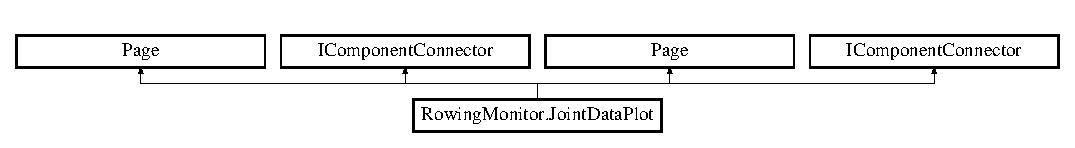
\includegraphics[height=1.538461cm]{class_rowing_monitor_1_1_joint_data_plot}
\end{center}
\end{figure}
\subsection*{Public Member Functions}
\begin{DoxyCompactItemize}
\item 
void \hyperlink{class_rowing_monitor_1_1_joint_data_plot_a8cfc1167162972427c71ab8247c1d19d}{Initialize\+Component} ()
\begin{DoxyCompactList}\small\item\em Initialize\+Component \end{DoxyCompactList}\item 
void \hyperlink{class_rowing_monitor_1_1_joint_data_plot_a8cfc1167162972427c71ab8247c1d19d}{Initialize\+Component} ()
\begin{DoxyCompactList}\small\item\em Initialize\+Component \end{DoxyCompactList}\end{DoxyCompactItemize}


\subsection{Detailed Description}
\hyperlink{class_rowing_monitor_1_1_joint_data_plot}{Joint\+Data\+Plot} 



\subsection{Member Function Documentation}
\mbox{\Hypertarget{class_rowing_monitor_1_1_joint_data_plot_a8cfc1167162972427c71ab8247c1d19d}\label{class_rowing_monitor_1_1_joint_data_plot_a8cfc1167162972427c71ab8247c1d19d}} 
\index{Rowing\+Monitor\+::\+Joint\+Data\+Plot@{Rowing\+Monitor\+::\+Joint\+Data\+Plot}!Initialize\+Component@{Initialize\+Component}}
\index{Initialize\+Component@{Initialize\+Component}!Rowing\+Monitor\+::\+Joint\+Data\+Plot@{Rowing\+Monitor\+::\+Joint\+Data\+Plot}}
\subsubsection{\texorpdfstring{Initialize\+Component()}{InitializeComponent()}\hspace{0.1cm}{\footnotesize\ttfamily [1/2]}}
{\footnotesize\ttfamily void Rowing\+Monitor.\+Joint\+Data\+Plot.\+Initialize\+Component (\begin{DoxyParamCaption}{ }\end{DoxyParamCaption})}



Initialize\+Component 

\mbox{\Hypertarget{class_rowing_monitor_1_1_joint_data_plot_a8cfc1167162972427c71ab8247c1d19d}\label{class_rowing_monitor_1_1_joint_data_plot_a8cfc1167162972427c71ab8247c1d19d}} 
\index{Rowing\+Monitor\+::\+Joint\+Data\+Plot@{Rowing\+Monitor\+::\+Joint\+Data\+Plot}!Initialize\+Component@{Initialize\+Component}}
\index{Initialize\+Component@{Initialize\+Component}!Rowing\+Monitor\+::\+Joint\+Data\+Plot@{Rowing\+Monitor\+::\+Joint\+Data\+Plot}}
\subsubsection{\texorpdfstring{Initialize\+Component()}{InitializeComponent()}\hspace{0.1cm}{\footnotesize\ttfamily [2/2]}}
{\footnotesize\ttfamily void Rowing\+Monitor.\+Joint\+Data\+Plot.\+Initialize\+Component (\begin{DoxyParamCaption}{ }\end{DoxyParamCaption})}



Initialize\+Component 



The documentation for this class was generated from the following files\+:\begin{DoxyCompactItemize}
\item 
obj/\+Debug/\hyperlink{_joint_data_plot_8g_8i_8cs}{Joint\+Data\+Plot.\+g.\+i.\+cs}\item 
obj/\+Debug/\hyperlink{_debug_2_joint_data_plot_view_8g_8i_8cs}{Joint\+Data\+Plot\+View.\+g.\+i.\+cs}\end{DoxyCompactItemize}

\hypertarget{class_rowing_monitor_1_1_view_1_1_joint_data_plot_view}{}\section{Rowing\+Monitor.\+View.\+Joint\+Data\+Plot\+View Class Reference}
\label{class_rowing_monitor_1_1_view_1_1_joint_data_plot_view}\index{Rowing\+Monitor.\+View.\+Joint\+Data\+Plot\+View@{Rowing\+Monitor.\+View.\+Joint\+Data\+Plot\+View}}


\hyperlink{class_rowing_monitor_1_1_view_1_1_joint_data_plot_view}{Joint\+Data\+Plot\+View}  


Inheritance diagram for Rowing\+Monitor.\+View.\+Joint\+Data\+Plot\+View\+:\begin{figure}[H]
\begin{center}
\leavevmode
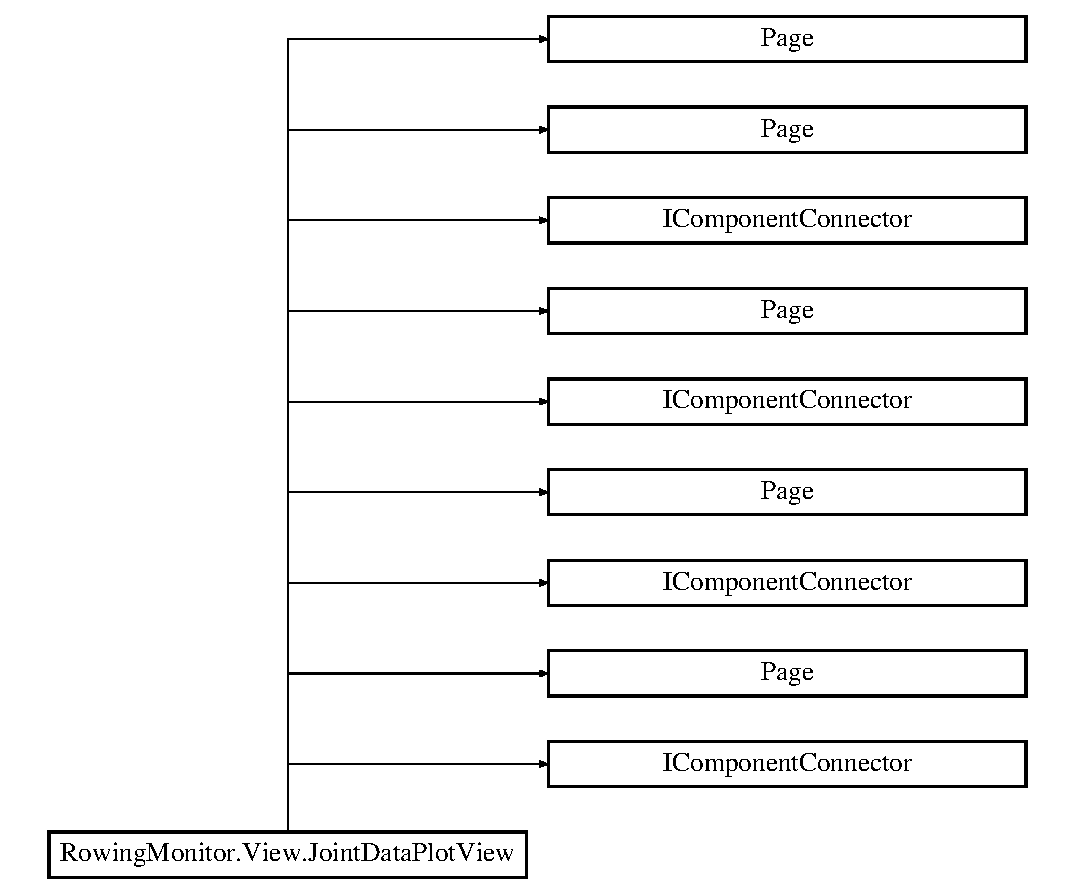
\includegraphics[height=10.000000cm]{class_rowing_monitor_1_1_view_1_1_joint_data_plot_view}
\end{center}
\end{figure}
\subsection*{Public Member Functions}
\begin{DoxyCompactItemize}
\item 
void \hyperlink{class_rowing_monitor_1_1_view_1_1_joint_data_plot_view_af935c9c9673d5672bb0359db871acc5d}{Initialize\+Component} ()
\begin{DoxyCompactList}\small\item\em Initialize\+Component \end{DoxyCompactList}\item 
void \hyperlink{class_rowing_monitor_1_1_view_1_1_joint_data_plot_view_af935c9c9673d5672bb0359db871acc5d}{Initialize\+Component} ()
\begin{DoxyCompactList}\small\item\em Initialize\+Component \end{DoxyCompactList}\item 
void \hyperlink{class_rowing_monitor_1_1_view_1_1_joint_data_plot_view_af935c9c9673d5672bb0359db871acc5d}{Initialize\+Component} ()
\begin{DoxyCompactList}\small\item\em Initialize\+Component \end{DoxyCompactList}\item 
void \hyperlink{class_rowing_monitor_1_1_view_1_1_joint_data_plot_view_af935c9c9673d5672bb0359db871acc5d}{Initialize\+Component} ()
\begin{DoxyCompactList}\small\item\em Initialize\+Component \end{DoxyCompactList}\item 
\hyperlink{class_rowing_monitor_1_1_view_1_1_joint_data_plot_view_a4b629e47777ec1c5a13c8e134a35ebb4}{Joint\+Data\+Plot\+View} ()
\end{DoxyCompactItemize}


\subsection{Detailed Description}
\hyperlink{class_rowing_monitor_1_1_view_1_1_joint_data_plot_view}{Joint\+Data\+Plot\+View} 

Interaktionslogik für Joint\+Data\+Plot\+View.\+xaml 

\subsection{Constructor \& Destructor Documentation}
\mbox{\Hypertarget{class_rowing_monitor_1_1_view_1_1_joint_data_plot_view_a4b629e47777ec1c5a13c8e134a35ebb4}\label{class_rowing_monitor_1_1_view_1_1_joint_data_plot_view_a4b629e47777ec1c5a13c8e134a35ebb4}} 
\index{Rowing\+Monitor\+::\+View\+::\+Joint\+Data\+Plot\+View@{Rowing\+Monitor\+::\+View\+::\+Joint\+Data\+Plot\+View}!Joint\+Data\+Plot\+View@{Joint\+Data\+Plot\+View}}
\index{Joint\+Data\+Plot\+View@{Joint\+Data\+Plot\+View}!Rowing\+Monitor\+::\+View\+::\+Joint\+Data\+Plot\+View@{Rowing\+Monitor\+::\+View\+::\+Joint\+Data\+Plot\+View}}
\subsubsection{\texorpdfstring{Joint\+Data\+Plot\+View()}{JointDataPlotView()}}
{\footnotesize\ttfamily Rowing\+Monitor.\+View.\+Joint\+Data\+Plot\+View.\+Joint\+Data\+Plot\+View (\begin{DoxyParamCaption}{ }\end{DoxyParamCaption})}



\subsection{Member Function Documentation}
\mbox{\Hypertarget{class_rowing_monitor_1_1_view_1_1_joint_data_plot_view_af935c9c9673d5672bb0359db871acc5d}\label{class_rowing_monitor_1_1_view_1_1_joint_data_plot_view_af935c9c9673d5672bb0359db871acc5d}} 
\index{Rowing\+Monitor\+::\+View\+::\+Joint\+Data\+Plot\+View@{Rowing\+Monitor\+::\+View\+::\+Joint\+Data\+Plot\+View}!Initialize\+Component@{Initialize\+Component}}
\index{Initialize\+Component@{Initialize\+Component}!Rowing\+Monitor\+::\+View\+::\+Joint\+Data\+Plot\+View@{Rowing\+Monitor\+::\+View\+::\+Joint\+Data\+Plot\+View}}
\subsubsection{\texorpdfstring{Initialize\+Component()}{InitializeComponent()}\hspace{0.1cm}{\footnotesize\ttfamily [1/4]}}
{\footnotesize\ttfamily void Rowing\+Monitor.\+View.\+Joint\+Data\+Plot\+View.\+Initialize\+Component (\begin{DoxyParamCaption}{ }\end{DoxyParamCaption})}



Initialize\+Component 

\mbox{\Hypertarget{class_rowing_monitor_1_1_view_1_1_joint_data_plot_view_af935c9c9673d5672bb0359db871acc5d}\label{class_rowing_monitor_1_1_view_1_1_joint_data_plot_view_af935c9c9673d5672bb0359db871acc5d}} 
\index{Rowing\+Monitor\+::\+View\+::\+Joint\+Data\+Plot\+View@{Rowing\+Monitor\+::\+View\+::\+Joint\+Data\+Plot\+View}!Initialize\+Component@{Initialize\+Component}}
\index{Initialize\+Component@{Initialize\+Component}!Rowing\+Monitor\+::\+View\+::\+Joint\+Data\+Plot\+View@{Rowing\+Monitor\+::\+View\+::\+Joint\+Data\+Plot\+View}}
\subsubsection{\texorpdfstring{Initialize\+Component()}{InitializeComponent()}\hspace{0.1cm}{\footnotesize\ttfamily [2/4]}}
{\footnotesize\ttfamily void Rowing\+Monitor.\+View.\+Joint\+Data\+Plot\+View.\+Initialize\+Component (\begin{DoxyParamCaption}{ }\end{DoxyParamCaption})}



Initialize\+Component 

\mbox{\Hypertarget{class_rowing_monitor_1_1_view_1_1_joint_data_plot_view_af935c9c9673d5672bb0359db871acc5d}\label{class_rowing_monitor_1_1_view_1_1_joint_data_plot_view_af935c9c9673d5672bb0359db871acc5d}} 
\index{Rowing\+Monitor\+::\+View\+::\+Joint\+Data\+Plot\+View@{Rowing\+Monitor\+::\+View\+::\+Joint\+Data\+Plot\+View}!Initialize\+Component@{Initialize\+Component}}
\index{Initialize\+Component@{Initialize\+Component}!Rowing\+Monitor\+::\+View\+::\+Joint\+Data\+Plot\+View@{Rowing\+Monitor\+::\+View\+::\+Joint\+Data\+Plot\+View}}
\subsubsection{\texorpdfstring{Initialize\+Component()}{InitializeComponent()}\hspace{0.1cm}{\footnotesize\ttfamily [3/4]}}
{\footnotesize\ttfamily void Rowing\+Monitor.\+View.\+Joint\+Data\+Plot\+View.\+Initialize\+Component (\begin{DoxyParamCaption}{ }\end{DoxyParamCaption})}



Initialize\+Component 

\mbox{\Hypertarget{class_rowing_monitor_1_1_view_1_1_joint_data_plot_view_af935c9c9673d5672bb0359db871acc5d}\label{class_rowing_monitor_1_1_view_1_1_joint_data_plot_view_af935c9c9673d5672bb0359db871acc5d}} 
\index{Rowing\+Monitor\+::\+View\+::\+Joint\+Data\+Plot\+View@{Rowing\+Monitor\+::\+View\+::\+Joint\+Data\+Plot\+View}!Initialize\+Component@{Initialize\+Component}}
\index{Initialize\+Component@{Initialize\+Component}!Rowing\+Monitor\+::\+View\+::\+Joint\+Data\+Plot\+View@{Rowing\+Monitor\+::\+View\+::\+Joint\+Data\+Plot\+View}}
\subsubsection{\texorpdfstring{Initialize\+Component()}{InitializeComponent()}\hspace{0.1cm}{\footnotesize\ttfamily [4/4]}}
{\footnotesize\ttfamily void Rowing\+Monitor.\+View.\+Joint\+Data\+Plot\+View.\+Initialize\+Component (\begin{DoxyParamCaption}{ }\end{DoxyParamCaption})}



Initialize\+Component 



The documentation for this class was generated from the following files\+:\begin{DoxyCompactItemize}
\item 
obj/\+Debug/\+View/\hyperlink{_debug_2_view_2_joint_data_plot_view_8g_8cs}{Joint\+Data\+Plot\+View.\+g.\+cs}\item 
obj/\+Debug/\+View/\hyperlink{_debug_2_view_2_joint_data_plot_view_8g_8i_8cs}{Joint\+Data\+Plot\+View.\+g.\+i.\+cs}\item 
View/\hyperlink{_joint_data_plot_view_8xaml_8cs}{Joint\+Data\+Plot\+View.\+xaml.\+cs}\end{DoxyCompactItemize}

\hypertarget{class_rowing_monitor_1_1_view_model_1_1_joint_data_plot_view_model}{}\section{Rowing\+Monitor.\+View\+Model.\+Joint\+Data\+Plot\+View\+Model Class Reference}
\label{class_rowing_monitor_1_1_view_model_1_1_joint_data_plot_view_model}\index{Rowing\+Monitor.\+View\+Model.\+Joint\+Data\+Plot\+View\+Model@{Rowing\+Monitor.\+View\+Model.\+Joint\+Data\+Plot\+View\+Model}}
Inheritance diagram for Rowing\+Monitor.\+View\+Model.\+Joint\+Data\+Plot\+View\+Model\+:\begin{figure}[H]
\begin{center}
\leavevmode
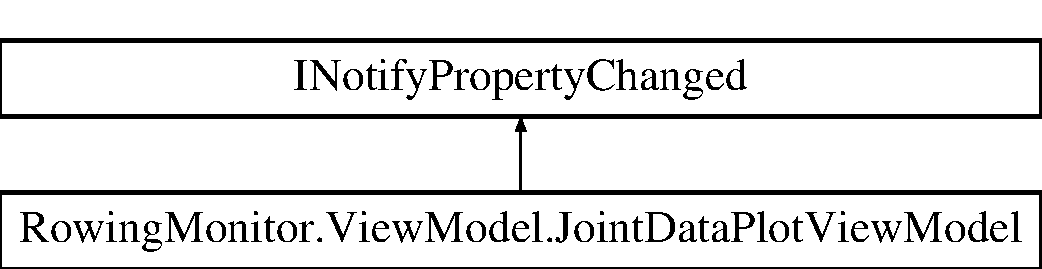
\includegraphics[height=2.000000cm]{class_rowing_monitor_1_1_view_model_1_1_joint_data_plot_view_model}
\end{center}
\end{figure}
\subsection*{Public Member Functions}
\begin{DoxyCompactItemize}
\item 
\hyperlink{class_rowing_monitor_1_1_view_model_1_1_joint_data_plot_view_model_a0617e5a1a406a41c3c0c0efb38fc4544}{Joint\+Data\+Plot\+View\+Model} ()
\item 
void \hyperlink{class_rowing_monitor_1_1_view_model_1_1_joint_data_plot_view_model_a7ade73f5c7afaf03a13fdf3839169a96}{Render} ()
\item 
void \hyperlink{class_rowing_monitor_1_1_view_model_1_1_joint_data_plot_view_model_a3b5455dd7cdb0c4309c8fe410d438abe}{Update} (\hyperlink{class_rowing_monitor_1_1_view_model_1_1_joint_data_plot_view_model_a68e8da622523739caafdfb6da1d9d112}{Plot\+Model} plot\+Model)
\end{DoxyCompactItemize}
\subsection*{Properties}
\begin{DoxyCompactItemize}
\item 
Plot\+Model \hyperlink{class_rowing_monitor_1_1_view_model_1_1_joint_data_plot_view_model_a68e8da622523739caafdfb6da1d9d112}{Plot\+Model}\hspace{0.3cm}{\ttfamily  \mbox{[}get, set\mbox{]}}
\begin{DoxyCompactList}\small\item\em Represents the plot. \end{DoxyCompactList}\end{DoxyCompactItemize}
\subsection*{Events}
\begin{DoxyCompactItemize}
\item 
Property\+Changed\+Event\+Handler \hyperlink{class_rowing_monitor_1_1_view_model_1_1_joint_data_plot_view_model_ae2148e9e8b2dbb242f0a4cff6265e837}{Property\+Changed}
\end{DoxyCompactItemize}


\subsection{Constructor \& Destructor Documentation}
\mbox{\Hypertarget{class_rowing_monitor_1_1_view_model_1_1_joint_data_plot_view_model_a0617e5a1a406a41c3c0c0efb38fc4544}\label{class_rowing_monitor_1_1_view_model_1_1_joint_data_plot_view_model_a0617e5a1a406a41c3c0c0efb38fc4544}} 
\index{Rowing\+Monitor\+::\+View\+Model\+::\+Joint\+Data\+Plot\+View\+Model@{Rowing\+Monitor\+::\+View\+Model\+::\+Joint\+Data\+Plot\+View\+Model}!Joint\+Data\+Plot\+View\+Model@{Joint\+Data\+Plot\+View\+Model}}
\index{Joint\+Data\+Plot\+View\+Model@{Joint\+Data\+Plot\+View\+Model}!Rowing\+Monitor\+::\+View\+Model\+::\+Joint\+Data\+Plot\+View\+Model@{Rowing\+Monitor\+::\+View\+Model\+::\+Joint\+Data\+Plot\+View\+Model}}
\subsubsection{\texorpdfstring{Joint\+Data\+Plot\+View\+Model()}{JointDataPlotViewModel()}}
{\footnotesize\ttfamily Rowing\+Monitor.\+View\+Model.\+Joint\+Data\+Plot\+View\+Model.\+Joint\+Data\+Plot\+View\+Model (\begin{DoxyParamCaption}{ }\end{DoxyParamCaption})}



\subsection{Member Function Documentation}
\mbox{\Hypertarget{class_rowing_monitor_1_1_view_model_1_1_joint_data_plot_view_model_a7ade73f5c7afaf03a13fdf3839169a96}\label{class_rowing_monitor_1_1_view_model_1_1_joint_data_plot_view_model_a7ade73f5c7afaf03a13fdf3839169a96}} 
\index{Rowing\+Monitor\+::\+View\+Model\+::\+Joint\+Data\+Plot\+View\+Model@{Rowing\+Monitor\+::\+View\+Model\+::\+Joint\+Data\+Plot\+View\+Model}!Render@{Render}}
\index{Render@{Render}!Rowing\+Monitor\+::\+View\+Model\+::\+Joint\+Data\+Plot\+View\+Model@{Rowing\+Monitor\+::\+View\+Model\+::\+Joint\+Data\+Plot\+View\+Model}}
\subsubsection{\texorpdfstring{Render()}{Render()}}
{\footnotesize\ttfamily void Rowing\+Monitor.\+View\+Model.\+Joint\+Data\+Plot\+View\+Model.\+Render (\begin{DoxyParamCaption}{ }\end{DoxyParamCaption})}

\mbox{\Hypertarget{class_rowing_monitor_1_1_view_model_1_1_joint_data_plot_view_model_a3b5455dd7cdb0c4309c8fe410d438abe}\label{class_rowing_monitor_1_1_view_model_1_1_joint_data_plot_view_model_a3b5455dd7cdb0c4309c8fe410d438abe}} 
\index{Rowing\+Monitor\+::\+View\+Model\+::\+Joint\+Data\+Plot\+View\+Model@{Rowing\+Monitor\+::\+View\+Model\+::\+Joint\+Data\+Plot\+View\+Model}!Update@{Update}}
\index{Update@{Update}!Rowing\+Monitor\+::\+View\+Model\+::\+Joint\+Data\+Plot\+View\+Model@{Rowing\+Monitor\+::\+View\+Model\+::\+Joint\+Data\+Plot\+View\+Model}}
\subsubsection{\texorpdfstring{Update()}{Update()}}
{\footnotesize\ttfamily void Rowing\+Monitor.\+View\+Model.\+Joint\+Data\+Plot\+View\+Model.\+Update (\begin{DoxyParamCaption}\item[{\hyperlink{class_rowing_monitor_1_1_view_model_1_1_joint_data_plot_view_model_a68e8da622523739caafdfb6da1d9d112}{Plot\+Model}}]{plot\+Model }\end{DoxyParamCaption})}



\subsection{Property Documentation}
\mbox{\Hypertarget{class_rowing_monitor_1_1_view_model_1_1_joint_data_plot_view_model_a68e8da622523739caafdfb6da1d9d112}\label{class_rowing_monitor_1_1_view_model_1_1_joint_data_plot_view_model_a68e8da622523739caafdfb6da1d9d112}} 
\index{Rowing\+Monitor\+::\+View\+Model\+::\+Joint\+Data\+Plot\+View\+Model@{Rowing\+Monitor\+::\+View\+Model\+::\+Joint\+Data\+Plot\+View\+Model}!Plot\+Model@{Plot\+Model}}
\index{Plot\+Model@{Plot\+Model}!Rowing\+Monitor\+::\+View\+Model\+::\+Joint\+Data\+Plot\+View\+Model@{Rowing\+Monitor\+::\+View\+Model\+::\+Joint\+Data\+Plot\+View\+Model}}
\subsubsection{\texorpdfstring{Plot\+Model}{PlotModel}}
{\footnotesize\ttfamily Plot\+Model Rowing\+Monitor.\+View\+Model.\+Joint\+Data\+Plot\+View\+Model.\+Plot\+Model\hspace{0.3cm}{\ttfamily [get]}, {\ttfamily [set]}}



Represents the plot. 



\subsection{Event Documentation}
\mbox{\Hypertarget{class_rowing_monitor_1_1_view_model_1_1_joint_data_plot_view_model_ae2148e9e8b2dbb242f0a4cff6265e837}\label{class_rowing_monitor_1_1_view_model_1_1_joint_data_plot_view_model_ae2148e9e8b2dbb242f0a4cff6265e837}} 
\index{Rowing\+Monitor\+::\+View\+Model\+::\+Joint\+Data\+Plot\+View\+Model@{Rowing\+Monitor\+::\+View\+Model\+::\+Joint\+Data\+Plot\+View\+Model}!Property\+Changed@{Property\+Changed}}
\index{Property\+Changed@{Property\+Changed}!Rowing\+Monitor\+::\+View\+Model\+::\+Joint\+Data\+Plot\+View\+Model@{Rowing\+Monitor\+::\+View\+Model\+::\+Joint\+Data\+Plot\+View\+Model}}
\subsubsection{\texorpdfstring{Property\+Changed}{PropertyChanged}}
{\footnotesize\ttfamily Property\+Changed\+Event\+Handler Rowing\+Monitor.\+View\+Model.\+Joint\+Data\+Plot\+View\+Model.\+Property\+Changed}



The documentation for this class was generated from the following file\+:\begin{DoxyCompactItemize}
\item 
View\+Model/\hyperlink{_joint_data_plot_view_model_8cs}{Joint\+Data\+Plot\+View\+Model.\+cs}\end{DoxyCompactItemize}

\hypertarget{class_rowing_monitor_1_1_model_1_1_kinect_frame_arrived_event_args}{}\section{Rowing\+Monitor.\+Model.\+Kinect\+Frame\+Arrived\+Event\+Args Class Reference}
\label{class_rowing_monitor_1_1_model_1_1_kinect_frame_arrived_event_args}\index{Rowing\+Monitor.\+Model.\+Kinect\+Frame\+Arrived\+Event\+Args@{Rowing\+Monitor.\+Model.\+Kinect\+Frame\+Arrived\+Event\+Args}}


Represents the arguments for a Kinect\+Reader\textquotesingle{}s Frame\+Arrived event.  


Inheritance diagram for Rowing\+Monitor.\+Model.\+Kinect\+Frame\+Arrived\+Event\+Args\+:\begin{figure}[H]
\begin{center}
\leavevmode
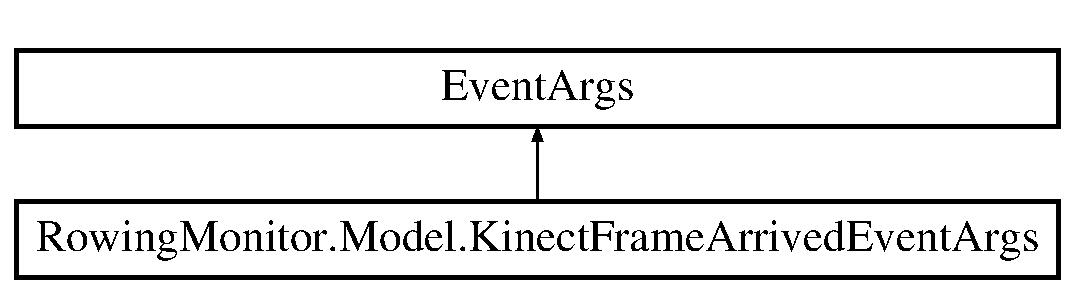
\includegraphics[height=2.000000cm]{class_rowing_monitor_1_1_model_1_1_kinect_frame_arrived_event_args}
\end{center}
\end{figure}
\subsection*{Public Member Functions}
\begin{DoxyCompactItemize}
\item 
\hyperlink{class_rowing_monitor_1_1_model_1_1_kinect_frame_arrived_event_args_a6c0155b21bc19c9fe163c5ea9ef66b21}{Kinect\+Frame\+Arrived\+Event\+Args} (\hyperlink{struct_rowing_monitor_1_1_model_1_1_util_1_1_joint_data}{Joint\+Data} joint\+Data)
\end{DoxyCompactItemize}
\subsection*{Properties}
\begin{DoxyCompactItemize}
\item 
\hyperlink{struct_rowing_monitor_1_1_model_1_1_util_1_1_joint_data}{Joint\+Data} \hyperlink{class_rowing_monitor_1_1_model_1_1_kinect_frame_arrived_event_args_a2249c19be25bb9b2c3627fb1bfa7512b}{Joint\+Data}\hspace{0.3cm}{\ttfamily  \mbox{[}get\mbox{]}}
\end{DoxyCompactItemize}


\subsection{Detailed Description}
Represents the arguments for a Kinect\+Reader\textquotesingle{}s Frame\+Arrived event. 



\subsection{Constructor \& Destructor Documentation}
\mbox{\Hypertarget{class_rowing_monitor_1_1_model_1_1_kinect_frame_arrived_event_args_a6c0155b21bc19c9fe163c5ea9ef66b21}\label{class_rowing_monitor_1_1_model_1_1_kinect_frame_arrived_event_args_a6c0155b21bc19c9fe163c5ea9ef66b21}} 
\index{Rowing\+Monitor\+::\+Model\+::\+Kinect\+Frame\+Arrived\+Event\+Args@{Rowing\+Monitor\+::\+Model\+::\+Kinect\+Frame\+Arrived\+Event\+Args}!Kinect\+Frame\+Arrived\+Event\+Args@{Kinect\+Frame\+Arrived\+Event\+Args}}
\index{Kinect\+Frame\+Arrived\+Event\+Args@{Kinect\+Frame\+Arrived\+Event\+Args}!Rowing\+Monitor\+::\+Model\+::\+Kinect\+Frame\+Arrived\+Event\+Args@{Rowing\+Monitor\+::\+Model\+::\+Kinect\+Frame\+Arrived\+Event\+Args}}
\subsubsection{\texorpdfstring{Kinect\+Frame\+Arrived\+Event\+Args()}{KinectFrameArrivedEventArgs()}}
{\footnotesize\ttfamily Rowing\+Monitor.\+Model.\+Kinect\+Frame\+Arrived\+Event\+Args.\+Kinect\+Frame\+Arrived\+Event\+Args (\begin{DoxyParamCaption}\item[{\hyperlink{struct_rowing_monitor_1_1_model_1_1_util_1_1_joint_data}{Joint\+Data}}]{joint\+Data }\end{DoxyParamCaption})}



\subsection{Property Documentation}
\mbox{\Hypertarget{class_rowing_monitor_1_1_model_1_1_kinect_frame_arrived_event_args_a2249c19be25bb9b2c3627fb1bfa7512b}\label{class_rowing_monitor_1_1_model_1_1_kinect_frame_arrived_event_args_a2249c19be25bb9b2c3627fb1bfa7512b}} 
\index{Rowing\+Monitor\+::\+Model\+::\+Kinect\+Frame\+Arrived\+Event\+Args@{Rowing\+Monitor\+::\+Model\+::\+Kinect\+Frame\+Arrived\+Event\+Args}!Joint\+Data@{Joint\+Data}}
\index{Joint\+Data@{Joint\+Data}!Rowing\+Monitor\+::\+Model\+::\+Kinect\+Frame\+Arrived\+Event\+Args@{Rowing\+Monitor\+::\+Model\+::\+Kinect\+Frame\+Arrived\+Event\+Args}}
\subsubsection{\texorpdfstring{Joint\+Data}{JointData}}
{\footnotesize\ttfamily \hyperlink{struct_rowing_monitor_1_1_model_1_1_util_1_1_joint_data}{Joint\+Data} Rowing\+Monitor.\+Model.\+Kinect\+Frame\+Arrived\+Event\+Args.\+Joint\+Data\hspace{0.3cm}{\ttfamily [get]}}



The documentation for this class was generated from the following file\+:\begin{DoxyCompactItemize}
\item 
Model/\+Event\+Args/\hyperlink{_kinect_frame_arrived_event_args_8cs}{Kinect\+Frame\+Arrived\+Event\+Args.\+cs}\end{DoxyCompactItemize}

\hypertarget{class_rowing_monitor_1_1_model_1_1_pipeline_1_1_kinect_joint_smoothing_filter}{}\section{Rowing\+Monitor.\+Model.\+Pipeline.\+Kinect\+Joint\+Smoothing\+Filter Class Reference}
\label{class_rowing_monitor_1_1_model_1_1_pipeline_1_1_kinect_joint_smoothing_filter}\index{Rowing\+Monitor.\+Model.\+Pipeline.\+Kinect\+Joint\+Smoothing\+Filter@{Rowing\+Monitor.\+Model.\+Pipeline.\+Kinect\+Joint\+Smoothing\+Filter}}


Adapted default Kinect smoothing filter to work with the pipeline. \href{https://social.msdn.microsoft.com/Forums/en-US/ffbc8ec7-7551-4462-88aa-2fab69eac38f/joint-smoothing-code-c-errors-in-kinectjointfilter-class?forum=kinectv2sdk}{\tt https\+://social.\+msdn.\+microsoft.\+com/\+Forums/en-\/\+U\+S/ffbc8ec7-\/7551-\/4462-\/88aa-\/2fab69eac38f/joint-\/smoothing-\/code-\/c-\/errors-\/in-\/kinectjointfilter-\/class?forum=kinectv2sdk}  


Inheritance diagram for Rowing\+Monitor.\+Model.\+Pipeline.\+Kinect\+Joint\+Smoothing\+Filter\+:\begin{figure}[H]
\begin{center}
\leavevmode
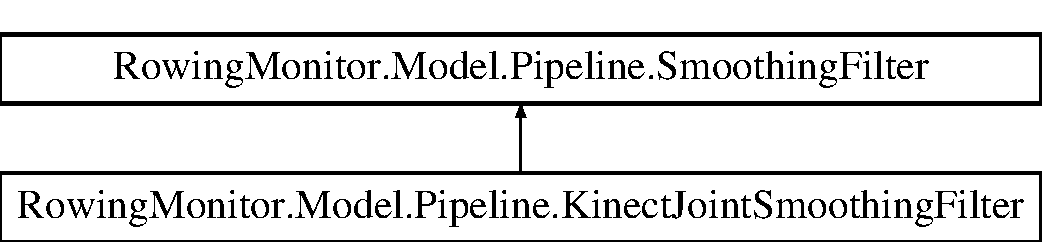
\includegraphics[height=2.000000cm]{class_rowing_monitor_1_1_model_1_1_pipeline_1_1_kinect_joint_smoothing_filter}
\end{center}
\end{figure}
\subsection*{Classes}
\begin{DoxyCompactItemize}
\item 
class \hyperlink{class_rowing_monitor_1_1_model_1_1_pipeline_1_1_kinect_joint_smoothing_filter_1_1_filter_double_exponential_data}{Filter\+Double\+Exponential\+Data}
\item 
struct \hyperlink{struct_rowing_monitor_1_1_model_1_1_pipeline_1_1_kinect_joint_smoothing_filter_1_1_t_r_a_n_s_f_o9fb8ee9e37e15ee7ab8d318a72b8984e}{T\+R\+A\+N\+S\+F\+O\+R\+M\+\_\+\+S\+M\+O\+O\+T\+H\+\_\+\+P\+A\+R\+A\+M\+E\+T\+E\+RS}
\end{DoxyCompactItemize}
\subsection*{Public Member Functions}
\begin{DoxyCompactItemize}
\item 
\hyperlink{class_rowing_monitor_1_1_model_1_1_pipeline_1_1_kinect_joint_smoothing_filter_a66e7c67626da3288c67427b6aa8f974b}{Kinect\+Joint\+Smoothing\+Filter} (\hyperlink{namespace_rowing_monitor_1_1_model_1_1_util_a01e1a06061533b246feb7421c9d0107f}{Data\+Stream\+Type} output\+Data\+Stream\+Type)
\item 
void \hyperlink{class_rowing_monitor_1_1_model_1_1_pipeline_1_1_kinect_joint_smoothing_filter_a77e9c9b72aeeb466af5d5f6791e1d568}{Init} (float f\+Smoothing=0.\+25f, float f\+Correction=0.\+25f, float f\+Prediction=0.\+25f, float f\+Jitter\+Radius=0.\+03f, float f\+Max\+Deviation\+Radius=0.\+05f)
\item 
void \hyperlink{class_rowing_monitor_1_1_model_1_1_pipeline_1_1_kinect_joint_smoothing_filter_a3f04af3eae0d014a73ac950c685b669b}{Shutdown} ()
\item 
void \hyperlink{class_rowing_monitor_1_1_model_1_1_pipeline_1_1_kinect_joint_smoothing_filter_a47c8d921b68fbf92a773a83c9ab602b7}{Reset} (float f\+Smoothing=0.\+25f, float f\+Correction=0.\+25f, float f\+Prediction=0.\+25f, float f\+Jitter\+Radius=0.\+03f, float f\+Max\+Deviation\+Radius=0.\+05f)
\item 
override void \hyperlink{class_rowing_monitor_1_1_model_1_1_pipeline_1_1_kinect_joint_smoothing_filter_a93cb6db0e00796dd2791789e472457b5}{Update} (\hyperlink{struct_rowing_monitor_1_1_model_1_1_util_1_1_joint_data}{Joint\+Data} joint\+Data)
\item 
Camera\+Space\+Point \mbox{[}$\,$\mbox{]} \hyperlink{class_rowing_monitor_1_1_model_1_1_pipeline_1_1_kinect_joint_smoothing_filter_aac138f87f70caab7b0c14071b52e84c7}{Get\+Filtered\+Joints} ()
\item 
override \hyperlink{struct_rowing_monitor_1_1_model_1_1_util_1_1_joint_data}{Joint\+Data} \hyperlink{class_rowing_monitor_1_1_model_1_1_pipeline_1_1_kinect_joint_smoothing_filter_a31ee74610f6c7de082306691f59d2f1c}{Smooth} (\hyperlink{struct_rowing_monitor_1_1_model_1_1_util_1_1_joint_data}{Joint\+Data} joint\+Data)
\end{DoxyCompactItemize}
\subsection*{Protected Member Functions}
\begin{DoxyCompactItemize}
\item 
override void \hyperlink{class_rowing_monitor_1_1_model_1_1_pipeline_1_1_kinect_joint_smoothing_filter_a944294caee0b2b26c0023a1c2d0c1a67}{On\+Smoothed\+Frame\+Finished} (\hyperlink{class_rowing_monitor_1_1_model_1_1_smoothed_frame_arrived_event_args}{Smoothed\+Frame\+Arrived\+Event\+Args} e)
\end{DoxyCompactItemize}
\subsection*{Additional Inherited Members}


\subsection{Detailed Description}
Adapted default Kinect smoothing filter to work with the pipeline. \href{https://social.msdn.microsoft.com/Forums/en-US/ffbc8ec7-7551-4462-88aa-2fab69eac38f/joint-smoothing-code-c-errors-in-kinectjointfilter-class?forum=kinectv2sdk}{\tt https\+://social.\+msdn.\+microsoft.\+com/\+Forums/en-\/\+U\+S/ffbc8ec7-\/7551-\/4462-\/88aa-\/2fab69eac38f/joint-\/smoothing-\/code-\/c-\/errors-\/in-\/kinectjointfilter-\/class?forum=kinectv2sdk} 



\subsection{Constructor \& Destructor Documentation}
\mbox{\Hypertarget{class_rowing_monitor_1_1_model_1_1_pipeline_1_1_kinect_joint_smoothing_filter_a66e7c67626da3288c67427b6aa8f974b}\label{class_rowing_monitor_1_1_model_1_1_pipeline_1_1_kinect_joint_smoothing_filter_a66e7c67626da3288c67427b6aa8f974b}} 
\index{Rowing\+Monitor\+::\+Model\+::\+Pipeline\+::\+Kinect\+Joint\+Smoothing\+Filter@{Rowing\+Monitor\+::\+Model\+::\+Pipeline\+::\+Kinect\+Joint\+Smoothing\+Filter}!Kinect\+Joint\+Smoothing\+Filter@{Kinect\+Joint\+Smoothing\+Filter}}
\index{Kinect\+Joint\+Smoothing\+Filter@{Kinect\+Joint\+Smoothing\+Filter}!Rowing\+Monitor\+::\+Model\+::\+Pipeline\+::\+Kinect\+Joint\+Smoothing\+Filter@{Rowing\+Monitor\+::\+Model\+::\+Pipeline\+::\+Kinect\+Joint\+Smoothing\+Filter}}
\subsubsection{\texorpdfstring{Kinect\+Joint\+Smoothing\+Filter()}{KinectJointSmoothingFilter()}}
{\footnotesize\ttfamily Rowing\+Monitor.\+Model.\+Pipeline.\+Kinect\+Joint\+Smoothing\+Filter.\+Kinect\+Joint\+Smoothing\+Filter (\begin{DoxyParamCaption}\item[{\hyperlink{namespace_rowing_monitor_1_1_model_1_1_util_a01e1a06061533b246feb7421c9d0107f}{Data\+Stream\+Type}}]{output\+Data\+Stream\+Type }\end{DoxyParamCaption})}



\subsection{Member Function Documentation}
\mbox{\Hypertarget{class_rowing_monitor_1_1_model_1_1_pipeline_1_1_kinect_joint_smoothing_filter_aac138f87f70caab7b0c14071b52e84c7}\label{class_rowing_monitor_1_1_model_1_1_pipeline_1_1_kinect_joint_smoothing_filter_aac138f87f70caab7b0c14071b52e84c7}} 
\index{Rowing\+Monitor\+::\+Model\+::\+Pipeline\+::\+Kinect\+Joint\+Smoothing\+Filter@{Rowing\+Monitor\+::\+Model\+::\+Pipeline\+::\+Kinect\+Joint\+Smoothing\+Filter}!Get\+Filtered\+Joints@{Get\+Filtered\+Joints}}
\index{Get\+Filtered\+Joints@{Get\+Filtered\+Joints}!Rowing\+Monitor\+::\+Model\+::\+Pipeline\+::\+Kinect\+Joint\+Smoothing\+Filter@{Rowing\+Monitor\+::\+Model\+::\+Pipeline\+::\+Kinect\+Joint\+Smoothing\+Filter}}
\subsubsection{\texorpdfstring{Get\+Filtered\+Joints()}{GetFilteredJoints()}}
{\footnotesize\ttfamily Camera\+Space\+Point \mbox{[}$\,$\mbox{]} Rowing\+Monitor.\+Model.\+Pipeline.\+Kinect\+Joint\+Smoothing\+Filter.\+Get\+Filtered\+Joints (\begin{DoxyParamCaption}{ }\end{DoxyParamCaption})}

\mbox{\Hypertarget{class_rowing_monitor_1_1_model_1_1_pipeline_1_1_kinect_joint_smoothing_filter_a77e9c9b72aeeb466af5d5f6791e1d568}\label{class_rowing_monitor_1_1_model_1_1_pipeline_1_1_kinect_joint_smoothing_filter_a77e9c9b72aeeb466af5d5f6791e1d568}} 
\index{Rowing\+Monitor\+::\+Model\+::\+Pipeline\+::\+Kinect\+Joint\+Smoothing\+Filter@{Rowing\+Monitor\+::\+Model\+::\+Pipeline\+::\+Kinect\+Joint\+Smoothing\+Filter}!Init@{Init}}
\index{Init@{Init}!Rowing\+Monitor\+::\+Model\+::\+Pipeline\+::\+Kinect\+Joint\+Smoothing\+Filter@{Rowing\+Monitor\+::\+Model\+::\+Pipeline\+::\+Kinect\+Joint\+Smoothing\+Filter}}
\subsubsection{\texorpdfstring{Init()}{Init()}}
{\footnotesize\ttfamily void Rowing\+Monitor.\+Model.\+Pipeline.\+Kinect\+Joint\+Smoothing\+Filter.\+Init (\begin{DoxyParamCaption}\item[{float}]{f\+Smoothing = {\ttfamily 0.25f},  }\item[{float}]{f\+Correction = {\ttfamily 0.25f},  }\item[{float}]{f\+Prediction = {\ttfamily 0.25f},  }\item[{float}]{f\+Jitter\+Radius = {\ttfamily 0.03f},  }\item[{float}]{f\+Max\+Deviation\+Radius = {\ttfamily 0.05f} }\end{DoxyParamCaption})}

\mbox{\Hypertarget{class_rowing_monitor_1_1_model_1_1_pipeline_1_1_kinect_joint_smoothing_filter_a944294caee0b2b26c0023a1c2d0c1a67}\label{class_rowing_monitor_1_1_model_1_1_pipeline_1_1_kinect_joint_smoothing_filter_a944294caee0b2b26c0023a1c2d0c1a67}} 
\index{Rowing\+Monitor\+::\+Model\+::\+Pipeline\+::\+Kinect\+Joint\+Smoothing\+Filter@{Rowing\+Monitor\+::\+Model\+::\+Pipeline\+::\+Kinect\+Joint\+Smoothing\+Filter}!On\+Smoothed\+Frame\+Finished@{On\+Smoothed\+Frame\+Finished}}
\index{On\+Smoothed\+Frame\+Finished@{On\+Smoothed\+Frame\+Finished}!Rowing\+Monitor\+::\+Model\+::\+Pipeline\+::\+Kinect\+Joint\+Smoothing\+Filter@{Rowing\+Monitor\+::\+Model\+::\+Pipeline\+::\+Kinect\+Joint\+Smoothing\+Filter}}
\subsubsection{\texorpdfstring{On\+Smoothed\+Frame\+Finished()}{OnSmoothedFrameFinished()}}
{\footnotesize\ttfamily override void Rowing\+Monitor.\+Model.\+Pipeline.\+Kinect\+Joint\+Smoothing\+Filter.\+On\+Smoothed\+Frame\+Finished (\begin{DoxyParamCaption}\item[{\hyperlink{class_rowing_monitor_1_1_model_1_1_smoothed_frame_arrived_event_args}{Smoothed\+Frame\+Arrived\+Event\+Args}}]{e }\end{DoxyParamCaption})\hspace{0.3cm}{\ttfamily [protected]}, {\ttfamily [virtual]}}



Reimplemented from \hyperlink{class_rowing_monitor_1_1_model_1_1_pipeline_1_1_smoothing_filter_ac47b399ad4ae1ad899f5e571d6f6c05c}{Rowing\+Monitor.\+Model.\+Pipeline.\+Smoothing\+Filter}.

\mbox{\Hypertarget{class_rowing_monitor_1_1_model_1_1_pipeline_1_1_kinect_joint_smoothing_filter_a47c8d921b68fbf92a773a83c9ab602b7}\label{class_rowing_monitor_1_1_model_1_1_pipeline_1_1_kinect_joint_smoothing_filter_a47c8d921b68fbf92a773a83c9ab602b7}} 
\index{Rowing\+Monitor\+::\+Model\+::\+Pipeline\+::\+Kinect\+Joint\+Smoothing\+Filter@{Rowing\+Monitor\+::\+Model\+::\+Pipeline\+::\+Kinect\+Joint\+Smoothing\+Filter}!Reset@{Reset}}
\index{Reset@{Reset}!Rowing\+Monitor\+::\+Model\+::\+Pipeline\+::\+Kinect\+Joint\+Smoothing\+Filter@{Rowing\+Monitor\+::\+Model\+::\+Pipeline\+::\+Kinect\+Joint\+Smoothing\+Filter}}
\subsubsection{\texorpdfstring{Reset()}{Reset()}}
{\footnotesize\ttfamily void Rowing\+Monitor.\+Model.\+Pipeline.\+Kinect\+Joint\+Smoothing\+Filter.\+Reset (\begin{DoxyParamCaption}\item[{float}]{f\+Smoothing = {\ttfamily 0.25f},  }\item[{float}]{f\+Correction = {\ttfamily 0.25f},  }\item[{float}]{f\+Prediction = {\ttfamily 0.25f},  }\item[{float}]{f\+Jitter\+Radius = {\ttfamily 0.03f},  }\item[{float}]{f\+Max\+Deviation\+Radius = {\ttfamily 0.05f} }\end{DoxyParamCaption})}

\mbox{\Hypertarget{class_rowing_monitor_1_1_model_1_1_pipeline_1_1_kinect_joint_smoothing_filter_a3f04af3eae0d014a73ac950c685b669b}\label{class_rowing_monitor_1_1_model_1_1_pipeline_1_1_kinect_joint_smoothing_filter_a3f04af3eae0d014a73ac950c685b669b}} 
\index{Rowing\+Monitor\+::\+Model\+::\+Pipeline\+::\+Kinect\+Joint\+Smoothing\+Filter@{Rowing\+Monitor\+::\+Model\+::\+Pipeline\+::\+Kinect\+Joint\+Smoothing\+Filter}!Shutdown@{Shutdown}}
\index{Shutdown@{Shutdown}!Rowing\+Monitor\+::\+Model\+::\+Pipeline\+::\+Kinect\+Joint\+Smoothing\+Filter@{Rowing\+Monitor\+::\+Model\+::\+Pipeline\+::\+Kinect\+Joint\+Smoothing\+Filter}}
\subsubsection{\texorpdfstring{Shutdown()}{Shutdown()}}
{\footnotesize\ttfamily void Rowing\+Monitor.\+Model.\+Pipeline.\+Kinect\+Joint\+Smoothing\+Filter.\+Shutdown (\begin{DoxyParamCaption}{ }\end{DoxyParamCaption})}

\mbox{\Hypertarget{class_rowing_monitor_1_1_model_1_1_pipeline_1_1_kinect_joint_smoothing_filter_a31ee74610f6c7de082306691f59d2f1c}\label{class_rowing_monitor_1_1_model_1_1_pipeline_1_1_kinect_joint_smoothing_filter_a31ee74610f6c7de082306691f59d2f1c}} 
\index{Rowing\+Monitor\+::\+Model\+::\+Pipeline\+::\+Kinect\+Joint\+Smoothing\+Filter@{Rowing\+Monitor\+::\+Model\+::\+Pipeline\+::\+Kinect\+Joint\+Smoothing\+Filter}!Smooth@{Smooth}}
\index{Smooth@{Smooth}!Rowing\+Monitor\+::\+Model\+::\+Pipeline\+::\+Kinect\+Joint\+Smoothing\+Filter@{Rowing\+Monitor\+::\+Model\+::\+Pipeline\+::\+Kinect\+Joint\+Smoothing\+Filter}}
\subsubsection{\texorpdfstring{Smooth()}{Smooth()}}
{\footnotesize\ttfamily override \hyperlink{struct_rowing_monitor_1_1_model_1_1_util_1_1_joint_data}{Joint\+Data} Rowing\+Monitor.\+Model.\+Pipeline.\+Kinect\+Joint\+Smoothing\+Filter.\+Smooth (\begin{DoxyParamCaption}\item[{\hyperlink{struct_rowing_monitor_1_1_model_1_1_util_1_1_joint_data}{Joint\+Data}}]{joint\+Data }\end{DoxyParamCaption})\hspace{0.3cm}{\ttfamily [virtual]}}



Implements \hyperlink{class_rowing_monitor_1_1_model_1_1_pipeline_1_1_smoothing_filter_a65ba6a5a48fbf5a51fb564dbeefc95fe}{Rowing\+Monitor.\+Model.\+Pipeline.\+Smoothing\+Filter}.

\mbox{\Hypertarget{class_rowing_monitor_1_1_model_1_1_pipeline_1_1_kinect_joint_smoothing_filter_a93cb6db0e00796dd2791789e472457b5}\label{class_rowing_monitor_1_1_model_1_1_pipeline_1_1_kinect_joint_smoothing_filter_a93cb6db0e00796dd2791789e472457b5}} 
\index{Rowing\+Monitor\+::\+Model\+::\+Pipeline\+::\+Kinect\+Joint\+Smoothing\+Filter@{Rowing\+Monitor\+::\+Model\+::\+Pipeline\+::\+Kinect\+Joint\+Smoothing\+Filter}!Update@{Update}}
\index{Update@{Update}!Rowing\+Monitor\+::\+Model\+::\+Pipeline\+::\+Kinect\+Joint\+Smoothing\+Filter@{Rowing\+Monitor\+::\+Model\+::\+Pipeline\+::\+Kinect\+Joint\+Smoothing\+Filter}}
\subsubsection{\texorpdfstring{Update()}{Update()}}
{\footnotesize\ttfamily override void Rowing\+Monitor.\+Model.\+Pipeline.\+Kinect\+Joint\+Smoothing\+Filter.\+Update (\begin{DoxyParamCaption}\item[{\hyperlink{struct_rowing_monitor_1_1_model_1_1_util_1_1_joint_data}{Joint\+Data}}]{joint\+Data }\end{DoxyParamCaption})\hspace{0.3cm}{\ttfamily [virtual]}}



Implements \hyperlink{class_rowing_monitor_1_1_model_1_1_pipeline_1_1_smoothing_filter_a6f017782fee0747d4ece9ec3ffea6115}{Rowing\+Monitor.\+Model.\+Pipeline.\+Smoothing\+Filter}.



The documentation for this class was generated from the following file\+:\begin{DoxyCompactItemize}
\item 
Model/\+Pipeline/\hyperlink{_kinect_joint_smoothing_filter_8cs}{Kinect\+Joint\+Smoothing\+Filter.\+cs}\end{DoxyCompactItemize}

\hypertarget{class_rowing_monitor_1_1_model_1_1_pipeline_1_1_kinect_reader}{}\section{Rowing\+Monitor.\+Model.\+Pipeline.\+Kinect\+Reader Class Reference}
\label{class_rowing_monitor_1_1_model_1_1_pipeline_1_1_kinect_reader}\index{Rowing\+Monitor.\+Model.\+Pipeline.\+Kinect\+Reader@{Rowing\+Monitor.\+Model.\+Pipeline.\+Kinect\+Reader}}


The \hyperlink{class_rowing_monitor_1_1_model_1_1_pipeline_1_1_kinect_reader}{Kinect\+Reader} class connects the application to the Kinect device.  


\subsection*{Public Member Functions}
\begin{DoxyCompactItemize}
\item 
delegate void \hyperlink{class_rowing_monitor_1_1_model_1_1_pipeline_1_1_kinect_reader_a324ac8a3e20e308a754f163e0925e95a}{Kinect\+Frame\+Arrived\+Event\+Handler} (Object sender, \hyperlink{class_rowing_monitor_1_1_model_1_1_kinect_frame_arrived_event_args}{Kinect\+Frame\+Arrived\+Event\+Args} e)
\item 
delegate void \hyperlink{class_rowing_monitor_1_1_model_1_1_pipeline_1_1_kinect_reader_aefbafde39c2c91e3b57c1db7073198bc}{Color\+Frame\+Arrived\+Event\+Handler} (Object sender, \hyperlink{class_rowing_monitor_1_1_model_1_1_color_frame_arrived_event_args}{Color\+Frame\+Arrived\+Event\+Args} e)
\item 
void \hyperlink{class_rowing_monitor_1_1_model_1_1_pipeline_1_1_kinect_reader_a191df86e5b421857d4eed6a534738461}{Start\+Reader} ()
\begin{DoxyCompactList}\small\item\em Start the reader to aquire sensor data from the kinect sensor. \end{DoxyCompactList}\item 
void \hyperlink{class_rowing_monitor_1_1_model_1_1_pipeline_1_1_kinect_reader_a1beeef16207c67ed6a29d0c7b47b368d}{Stop\+Reader} ()
\begin{DoxyCompactList}\small\item\em Stop the kinect reader and clean up. \end{DoxyCompactList}\end{DoxyCompactItemize}
\subsection*{Properties}
\begin{DoxyCompactItemize}
\item 
Coordinate\+Mapper \hyperlink{class_rowing_monitor_1_1_model_1_1_pipeline_1_1_kinect_reader_abb848deb4ea9ed2ed53f6d95ce1945db}{Coordinate\+Mapper}\hspace{0.3cm}{\ttfamily  \mbox{[}get\mbox{]}}
\item 
string \hyperlink{class_rowing_monitor_1_1_model_1_1_pipeline_1_1_kinect_reader_a75073cd905041d0675f11e6ac23836bf}{Status\+Text}\hspace{0.3cm}{\ttfamily  \mbox{[}get\mbox{]}}
\item 
static \hyperlink{class_rowing_monitor_1_1_model_1_1_pipeline_1_1_kinect_reader}{Kinect\+Reader} \hyperlink{class_rowing_monitor_1_1_model_1_1_pipeline_1_1_kinect_reader_ae0ef04719102355582b9c41b5affed8c}{Instance}\hspace{0.3cm}{\ttfamily  \mbox{[}get\mbox{]}}
\begin{DoxyCompactList}\small\item\em Instance of \hyperlink{class_rowing_monitor_1_1_model_1_1_pipeline_1_1_kinect_reader}{Kinect\+Reader} singleton \end{DoxyCompactList}\item 
Broadcast\+Block$<$ \hyperlink{struct_rowing_monitor_1_1_model_1_1_util_1_1_joint_data}{Joint\+Data} $>$ \hyperlink{class_rowing_monitor_1_1_model_1_1_pipeline_1_1_kinect_reader_a6e860c115b12d8f17b8f800f9bc64645}{Joint\+Data\+Block}\hspace{0.3cm}{\ttfamily  \mbox{[}get\mbox{]}}
\item 
Broadcast\+Block$<$ Writeable\+Bitmap $>$ \hyperlink{class_rowing_monitor_1_1_model_1_1_pipeline_1_1_kinect_reader_acfc75a10c6a18c1a8f511944cb411937}{Color\+Frame\+Block}\hspace{0.3cm}{\ttfamily  \mbox{[}get\mbox{]}}
\item 
Frame\+Description \hyperlink{class_rowing_monitor_1_1_model_1_1_pipeline_1_1_kinect_reader_a8aafd70dd48e36b6cc55ad2bee4ae0e6}{Depth\+Frame\+Description}\hspace{0.3cm}{\ttfamily  \mbox{[}get\mbox{]}}
\item 
Frame\+Description \hyperlink{class_rowing_monitor_1_1_model_1_1_pipeline_1_1_kinect_reader_a43790d6bdb5e70d50c418fb17ac90ee6}{Color\+Frame\+Description}\hspace{0.3cm}{\ttfamily  \mbox{[}get\mbox{]}}
\end{DoxyCompactItemize}
\subsection*{Events}
\begin{DoxyCompactItemize}
\item 
\hyperlink{class_rowing_monitor_1_1_model_1_1_pipeline_1_1_kinect_reader_a324ac8a3e20e308a754f163e0925e95a}{Kinect\+Frame\+Arrived\+Event\+Handler} \hyperlink{class_rowing_monitor_1_1_model_1_1_pipeline_1_1_kinect_reader_a69f71477e3f769bab61917c3654b4965}{Kinect\+Frame\+Arrived}
\item 
\hyperlink{class_rowing_monitor_1_1_model_1_1_pipeline_1_1_kinect_reader_aefbafde39c2c91e3b57c1db7073198bc}{Color\+Frame\+Arrived\+Event\+Handler} \hyperlink{class_rowing_monitor_1_1_model_1_1_pipeline_1_1_kinect_reader_a5de5efaee2ef12948b7dfc6f8937b94d}{Color\+Frame\+Arrived}
\end{DoxyCompactItemize}


\subsection{Detailed Description}
The \hyperlink{class_rowing_monitor_1_1_model_1_1_pipeline_1_1_kinect_reader}{Kinect\+Reader} class connects the application to the Kinect device. 

This class uses the singleton pattern with static initialization. 

\subsection{Member Function Documentation}
\mbox{\Hypertarget{class_rowing_monitor_1_1_model_1_1_pipeline_1_1_kinect_reader_aefbafde39c2c91e3b57c1db7073198bc}\label{class_rowing_monitor_1_1_model_1_1_pipeline_1_1_kinect_reader_aefbafde39c2c91e3b57c1db7073198bc}} 
\index{Rowing\+Monitor\+::\+Model\+::\+Pipeline\+::\+Kinect\+Reader@{Rowing\+Monitor\+::\+Model\+::\+Pipeline\+::\+Kinect\+Reader}!Color\+Frame\+Arrived\+Event\+Handler@{Color\+Frame\+Arrived\+Event\+Handler}}
\index{Color\+Frame\+Arrived\+Event\+Handler@{Color\+Frame\+Arrived\+Event\+Handler}!Rowing\+Monitor\+::\+Model\+::\+Pipeline\+::\+Kinect\+Reader@{Rowing\+Monitor\+::\+Model\+::\+Pipeline\+::\+Kinect\+Reader}}
\subsubsection{\texorpdfstring{Color\+Frame\+Arrived\+Event\+Handler()}{ColorFrameArrivedEventHandler()}}
{\footnotesize\ttfamily delegate void Rowing\+Monitor.\+Model.\+Pipeline.\+Kinect\+Reader.\+Color\+Frame\+Arrived\+Event\+Handler (\begin{DoxyParamCaption}\item[{Object}]{sender,  }\item[{\hyperlink{class_rowing_monitor_1_1_model_1_1_color_frame_arrived_event_args}{Color\+Frame\+Arrived\+Event\+Args}}]{e }\end{DoxyParamCaption})}

\mbox{\Hypertarget{class_rowing_monitor_1_1_model_1_1_pipeline_1_1_kinect_reader_a324ac8a3e20e308a754f163e0925e95a}\label{class_rowing_monitor_1_1_model_1_1_pipeline_1_1_kinect_reader_a324ac8a3e20e308a754f163e0925e95a}} 
\index{Rowing\+Monitor\+::\+Model\+::\+Pipeline\+::\+Kinect\+Reader@{Rowing\+Monitor\+::\+Model\+::\+Pipeline\+::\+Kinect\+Reader}!Kinect\+Frame\+Arrived\+Event\+Handler@{Kinect\+Frame\+Arrived\+Event\+Handler}}
\index{Kinect\+Frame\+Arrived\+Event\+Handler@{Kinect\+Frame\+Arrived\+Event\+Handler}!Rowing\+Monitor\+::\+Model\+::\+Pipeline\+::\+Kinect\+Reader@{Rowing\+Monitor\+::\+Model\+::\+Pipeline\+::\+Kinect\+Reader}}
\subsubsection{\texorpdfstring{Kinect\+Frame\+Arrived\+Event\+Handler()}{KinectFrameArrivedEventHandler()}}
{\footnotesize\ttfamily delegate void Rowing\+Monitor.\+Model.\+Pipeline.\+Kinect\+Reader.\+Kinect\+Frame\+Arrived\+Event\+Handler (\begin{DoxyParamCaption}\item[{Object}]{sender,  }\item[{\hyperlink{class_rowing_monitor_1_1_model_1_1_kinect_frame_arrived_event_args}{Kinect\+Frame\+Arrived\+Event\+Args}}]{e }\end{DoxyParamCaption})}

\mbox{\Hypertarget{class_rowing_monitor_1_1_model_1_1_pipeline_1_1_kinect_reader_a191df86e5b421857d4eed6a534738461}\label{class_rowing_monitor_1_1_model_1_1_pipeline_1_1_kinect_reader_a191df86e5b421857d4eed6a534738461}} 
\index{Rowing\+Monitor\+::\+Model\+::\+Pipeline\+::\+Kinect\+Reader@{Rowing\+Monitor\+::\+Model\+::\+Pipeline\+::\+Kinect\+Reader}!Start\+Reader@{Start\+Reader}}
\index{Start\+Reader@{Start\+Reader}!Rowing\+Monitor\+::\+Model\+::\+Pipeline\+::\+Kinect\+Reader@{Rowing\+Monitor\+::\+Model\+::\+Pipeline\+::\+Kinect\+Reader}}
\subsubsection{\texorpdfstring{Start\+Reader()}{StartReader()}}
{\footnotesize\ttfamily void Rowing\+Monitor.\+Model.\+Pipeline.\+Kinect\+Reader.\+Start\+Reader (\begin{DoxyParamCaption}{ }\end{DoxyParamCaption})}



Start the reader to aquire sensor data from the kinect sensor. 

\mbox{\Hypertarget{class_rowing_monitor_1_1_model_1_1_pipeline_1_1_kinect_reader_a1beeef16207c67ed6a29d0c7b47b368d}\label{class_rowing_monitor_1_1_model_1_1_pipeline_1_1_kinect_reader_a1beeef16207c67ed6a29d0c7b47b368d}} 
\index{Rowing\+Monitor\+::\+Model\+::\+Pipeline\+::\+Kinect\+Reader@{Rowing\+Monitor\+::\+Model\+::\+Pipeline\+::\+Kinect\+Reader}!Stop\+Reader@{Stop\+Reader}}
\index{Stop\+Reader@{Stop\+Reader}!Rowing\+Monitor\+::\+Model\+::\+Pipeline\+::\+Kinect\+Reader@{Rowing\+Monitor\+::\+Model\+::\+Pipeline\+::\+Kinect\+Reader}}
\subsubsection{\texorpdfstring{Stop\+Reader()}{StopReader()}}
{\footnotesize\ttfamily void Rowing\+Monitor.\+Model.\+Pipeline.\+Kinect\+Reader.\+Stop\+Reader (\begin{DoxyParamCaption}{ }\end{DoxyParamCaption})}



Stop the kinect reader and clean up. 



\subsection{Property Documentation}
\mbox{\Hypertarget{class_rowing_monitor_1_1_model_1_1_pipeline_1_1_kinect_reader_acfc75a10c6a18c1a8f511944cb411937}\label{class_rowing_monitor_1_1_model_1_1_pipeline_1_1_kinect_reader_acfc75a10c6a18c1a8f511944cb411937}} 
\index{Rowing\+Monitor\+::\+Model\+::\+Pipeline\+::\+Kinect\+Reader@{Rowing\+Monitor\+::\+Model\+::\+Pipeline\+::\+Kinect\+Reader}!Color\+Frame\+Block@{Color\+Frame\+Block}}
\index{Color\+Frame\+Block@{Color\+Frame\+Block}!Rowing\+Monitor\+::\+Model\+::\+Pipeline\+::\+Kinect\+Reader@{Rowing\+Monitor\+::\+Model\+::\+Pipeline\+::\+Kinect\+Reader}}
\subsubsection{\texorpdfstring{Color\+Frame\+Block}{ColorFrameBlock}}
{\footnotesize\ttfamily Broadcast\+Block$<$Writeable\+Bitmap$>$ Rowing\+Monitor.\+Model.\+Pipeline.\+Kinect\+Reader.\+Color\+Frame\+Block\hspace{0.3cm}{\ttfamily [get]}}

\mbox{\Hypertarget{class_rowing_monitor_1_1_model_1_1_pipeline_1_1_kinect_reader_a43790d6bdb5e70d50c418fb17ac90ee6}\label{class_rowing_monitor_1_1_model_1_1_pipeline_1_1_kinect_reader_a43790d6bdb5e70d50c418fb17ac90ee6}} 
\index{Rowing\+Monitor\+::\+Model\+::\+Pipeline\+::\+Kinect\+Reader@{Rowing\+Monitor\+::\+Model\+::\+Pipeline\+::\+Kinect\+Reader}!Color\+Frame\+Description@{Color\+Frame\+Description}}
\index{Color\+Frame\+Description@{Color\+Frame\+Description}!Rowing\+Monitor\+::\+Model\+::\+Pipeline\+::\+Kinect\+Reader@{Rowing\+Monitor\+::\+Model\+::\+Pipeline\+::\+Kinect\+Reader}}
\subsubsection{\texorpdfstring{Color\+Frame\+Description}{ColorFrameDescription}}
{\footnotesize\ttfamily Frame\+Description Rowing\+Monitor.\+Model.\+Pipeline.\+Kinect\+Reader.\+Color\+Frame\+Description\hspace{0.3cm}{\ttfamily [get]}}

\mbox{\Hypertarget{class_rowing_monitor_1_1_model_1_1_pipeline_1_1_kinect_reader_abb848deb4ea9ed2ed53f6d95ce1945db}\label{class_rowing_monitor_1_1_model_1_1_pipeline_1_1_kinect_reader_abb848deb4ea9ed2ed53f6d95ce1945db}} 
\index{Rowing\+Monitor\+::\+Model\+::\+Pipeline\+::\+Kinect\+Reader@{Rowing\+Monitor\+::\+Model\+::\+Pipeline\+::\+Kinect\+Reader}!Coordinate\+Mapper@{Coordinate\+Mapper}}
\index{Coordinate\+Mapper@{Coordinate\+Mapper}!Rowing\+Monitor\+::\+Model\+::\+Pipeline\+::\+Kinect\+Reader@{Rowing\+Monitor\+::\+Model\+::\+Pipeline\+::\+Kinect\+Reader}}
\subsubsection{\texorpdfstring{Coordinate\+Mapper}{CoordinateMapper}}
{\footnotesize\ttfamily Coordinate\+Mapper Rowing\+Monitor.\+Model.\+Pipeline.\+Kinect\+Reader.\+Coordinate\+Mapper\hspace{0.3cm}{\ttfamily [get]}}

\mbox{\Hypertarget{class_rowing_monitor_1_1_model_1_1_pipeline_1_1_kinect_reader_a8aafd70dd48e36b6cc55ad2bee4ae0e6}\label{class_rowing_monitor_1_1_model_1_1_pipeline_1_1_kinect_reader_a8aafd70dd48e36b6cc55ad2bee4ae0e6}} 
\index{Rowing\+Monitor\+::\+Model\+::\+Pipeline\+::\+Kinect\+Reader@{Rowing\+Monitor\+::\+Model\+::\+Pipeline\+::\+Kinect\+Reader}!Depth\+Frame\+Description@{Depth\+Frame\+Description}}
\index{Depth\+Frame\+Description@{Depth\+Frame\+Description}!Rowing\+Monitor\+::\+Model\+::\+Pipeline\+::\+Kinect\+Reader@{Rowing\+Monitor\+::\+Model\+::\+Pipeline\+::\+Kinect\+Reader}}
\subsubsection{\texorpdfstring{Depth\+Frame\+Description}{DepthFrameDescription}}
{\footnotesize\ttfamily Frame\+Description Rowing\+Monitor.\+Model.\+Pipeline.\+Kinect\+Reader.\+Depth\+Frame\+Description\hspace{0.3cm}{\ttfamily [get]}}

\mbox{\Hypertarget{class_rowing_monitor_1_1_model_1_1_pipeline_1_1_kinect_reader_ae0ef04719102355582b9c41b5affed8c}\label{class_rowing_monitor_1_1_model_1_1_pipeline_1_1_kinect_reader_ae0ef04719102355582b9c41b5affed8c}} 
\index{Rowing\+Monitor\+::\+Model\+::\+Pipeline\+::\+Kinect\+Reader@{Rowing\+Monitor\+::\+Model\+::\+Pipeline\+::\+Kinect\+Reader}!Instance@{Instance}}
\index{Instance@{Instance}!Rowing\+Monitor\+::\+Model\+::\+Pipeline\+::\+Kinect\+Reader@{Rowing\+Monitor\+::\+Model\+::\+Pipeline\+::\+Kinect\+Reader}}
\subsubsection{\texorpdfstring{Instance}{Instance}}
{\footnotesize\ttfamily \hyperlink{class_rowing_monitor_1_1_model_1_1_pipeline_1_1_kinect_reader}{Kinect\+Reader} Rowing\+Monitor.\+Model.\+Pipeline.\+Kinect\+Reader.\+Instance\hspace{0.3cm}{\ttfamily [static]}, {\ttfamily [get]}}



Instance of \hyperlink{class_rowing_monitor_1_1_model_1_1_pipeline_1_1_kinect_reader}{Kinect\+Reader} singleton 

\mbox{\Hypertarget{class_rowing_monitor_1_1_model_1_1_pipeline_1_1_kinect_reader_a6e860c115b12d8f17b8f800f9bc64645}\label{class_rowing_monitor_1_1_model_1_1_pipeline_1_1_kinect_reader_a6e860c115b12d8f17b8f800f9bc64645}} 
\index{Rowing\+Monitor\+::\+Model\+::\+Pipeline\+::\+Kinect\+Reader@{Rowing\+Monitor\+::\+Model\+::\+Pipeline\+::\+Kinect\+Reader}!Joint\+Data\+Block@{Joint\+Data\+Block}}
\index{Joint\+Data\+Block@{Joint\+Data\+Block}!Rowing\+Monitor\+::\+Model\+::\+Pipeline\+::\+Kinect\+Reader@{Rowing\+Monitor\+::\+Model\+::\+Pipeline\+::\+Kinect\+Reader}}
\subsubsection{\texorpdfstring{Joint\+Data\+Block}{JointDataBlock}}
{\footnotesize\ttfamily Broadcast\+Block$<$\hyperlink{struct_rowing_monitor_1_1_model_1_1_util_1_1_joint_data}{Joint\+Data}$>$ Rowing\+Monitor.\+Model.\+Pipeline.\+Kinect\+Reader.\+Joint\+Data\+Block\hspace{0.3cm}{\ttfamily [get]}}

\mbox{\Hypertarget{class_rowing_monitor_1_1_model_1_1_pipeline_1_1_kinect_reader_a75073cd905041d0675f11e6ac23836bf}\label{class_rowing_monitor_1_1_model_1_1_pipeline_1_1_kinect_reader_a75073cd905041d0675f11e6ac23836bf}} 
\index{Rowing\+Monitor\+::\+Model\+::\+Pipeline\+::\+Kinect\+Reader@{Rowing\+Monitor\+::\+Model\+::\+Pipeline\+::\+Kinect\+Reader}!Status\+Text@{Status\+Text}}
\index{Status\+Text@{Status\+Text}!Rowing\+Monitor\+::\+Model\+::\+Pipeline\+::\+Kinect\+Reader@{Rowing\+Monitor\+::\+Model\+::\+Pipeline\+::\+Kinect\+Reader}}
\subsubsection{\texorpdfstring{Status\+Text}{StatusText}}
{\footnotesize\ttfamily string Rowing\+Monitor.\+Model.\+Pipeline.\+Kinect\+Reader.\+Status\+Text\hspace{0.3cm}{\ttfamily [get]}}



\subsection{Event Documentation}
\mbox{\Hypertarget{class_rowing_monitor_1_1_model_1_1_pipeline_1_1_kinect_reader_a5de5efaee2ef12948b7dfc6f8937b94d}\label{class_rowing_monitor_1_1_model_1_1_pipeline_1_1_kinect_reader_a5de5efaee2ef12948b7dfc6f8937b94d}} 
\index{Rowing\+Monitor\+::\+Model\+::\+Pipeline\+::\+Kinect\+Reader@{Rowing\+Monitor\+::\+Model\+::\+Pipeline\+::\+Kinect\+Reader}!Color\+Frame\+Arrived@{Color\+Frame\+Arrived}}
\index{Color\+Frame\+Arrived@{Color\+Frame\+Arrived}!Rowing\+Monitor\+::\+Model\+::\+Pipeline\+::\+Kinect\+Reader@{Rowing\+Monitor\+::\+Model\+::\+Pipeline\+::\+Kinect\+Reader}}
\subsubsection{\texorpdfstring{Color\+Frame\+Arrived}{ColorFrameArrived}}
{\footnotesize\ttfamily \hyperlink{class_rowing_monitor_1_1_model_1_1_pipeline_1_1_kinect_reader_aefbafde39c2c91e3b57c1db7073198bc}{Color\+Frame\+Arrived\+Event\+Handler} Rowing\+Monitor.\+Model.\+Pipeline.\+Kinect\+Reader.\+Color\+Frame\+Arrived}

\mbox{\Hypertarget{class_rowing_monitor_1_1_model_1_1_pipeline_1_1_kinect_reader_a69f71477e3f769bab61917c3654b4965}\label{class_rowing_monitor_1_1_model_1_1_pipeline_1_1_kinect_reader_a69f71477e3f769bab61917c3654b4965}} 
\index{Rowing\+Monitor\+::\+Model\+::\+Pipeline\+::\+Kinect\+Reader@{Rowing\+Monitor\+::\+Model\+::\+Pipeline\+::\+Kinect\+Reader}!Kinect\+Frame\+Arrived@{Kinect\+Frame\+Arrived}}
\index{Kinect\+Frame\+Arrived@{Kinect\+Frame\+Arrived}!Rowing\+Monitor\+::\+Model\+::\+Pipeline\+::\+Kinect\+Reader@{Rowing\+Monitor\+::\+Model\+::\+Pipeline\+::\+Kinect\+Reader}}
\subsubsection{\texorpdfstring{Kinect\+Frame\+Arrived}{KinectFrameArrived}}
{\footnotesize\ttfamily \hyperlink{class_rowing_monitor_1_1_model_1_1_pipeline_1_1_kinect_reader_a324ac8a3e20e308a754f163e0925e95a}{Kinect\+Frame\+Arrived\+Event\+Handler} Rowing\+Monitor.\+Model.\+Pipeline.\+Kinect\+Reader.\+Kinect\+Frame\+Arrived}



The documentation for this class was generated from the following file\+:\begin{DoxyCompactItemize}
\item 
Model/\+Pipeline/\hyperlink{_kinect_reader_8cs}{Kinect\+Reader.\+cs}\end{DoxyCompactItemize}

\hypertarget{struct_rowing_monitor_1_1_model_1_1_pipeline_1_1_kleshnev_data}{}\section{Rowing\+Monitor.\+Model.\+Pipeline.\+Kleshnev\+Data Struct Reference}
\label{struct_rowing_monitor_1_1_model_1_1_pipeline_1_1_kleshnev_data}\index{Rowing\+Monitor.\+Model.\+Pipeline.\+Kleshnev\+Data@{Rowing\+Monitor.\+Model.\+Pipeline.\+Kleshnev\+Data}}
\subsection*{Properties}
\begin{DoxyCompactItemize}
\item 
double \hyperlink{struct_rowing_monitor_1_1_model_1_1_pipeline_1_1_kleshnev_data_ab0f0ba7b2c4c9ec7248fca81c9a5f482}{Rel\+Timestamp}\hspace{0.3cm}{\ttfamily  \mbox{[}get, set\mbox{]}}
\item 
double \hyperlink{struct_rowing_monitor_1_1_model_1_1_pipeline_1_1_kleshnev_data_ad59fa89e9efe861ab2c0afd23297a62a}{Abs\+Timestamp}\hspace{0.3cm}{\ttfamily  \mbox{[}get, set\mbox{]}}
\item 
Dictionary$<$ \hyperlink{namespace_rowing_monitor_1_1_model_1_1_util_a45e0956b123d438555a1cb3997bd5cb4}{Kleshnev\+Velocity\+Type}, double $>$ \hyperlink{struct_rowing_monitor_1_1_model_1_1_pipeline_1_1_kleshnev_data_a62142432ba1620e06b133e9119b33493}{Velocities}\hspace{0.3cm}{\ttfamily  \mbox{[}get, set\mbox{]}}
\item 
long \hyperlink{struct_rowing_monitor_1_1_model_1_1_pipeline_1_1_kleshnev_data_a1b21f8ca17372b1da98a8f0126c5bcf2}{Index}\hspace{0.3cm}{\ttfamily  \mbox{[}get, set\mbox{]}}
\end{DoxyCompactItemize}


\subsection{Property Documentation}
\mbox{\Hypertarget{struct_rowing_monitor_1_1_model_1_1_pipeline_1_1_kleshnev_data_ad59fa89e9efe861ab2c0afd23297a62a}\label{struct_rowing_monitor_1_1_model_1_1_pipeline_1_1_kleshnev_data_ad59fa89e9efe861ab2c0afd23297a62a}} 
\index{Rowing\+Monitor\+::\+Model\+::\+Pipeline\+::\+Kleshnev\+Data@{Rowing\+Monitor\+::\+Model\+::\+Pipeline\+::\+Kleshnev\+Data}!Abs\+Timestamp@{Abs\+Timestamp}}
\index{Abs\+Timestamp@{Abs\+Timestamp}!Rowing\+Monitor\+::\+Model\+::\+Pipeline\+::\+Kleshnev\+Data@{Rowing\+Monitor\+::\+Model\+::\+Pipeline\+::\+Kleshnev\+Data}}
\subsubsection{\texorpdfstring{Abs\+Timestamp}{AbsTimestamp}}
{\footnotesize\ttfamily double Rowing\+Monitor.\+Model.\+Pipeline.\+Kleshnev\+Data.\+Abs\+Timestamp\hspace{0.3cm}{\ttfamily [get]}, {\ttfamily [set]}}

\mbox{\Hypertarget{struct_rowing_monitor_1_1_model_1_1_pipeline_1_1_kleshnev_data_a1b21f8ca17372b1da98a8f0126c5bcf2}\label{struct_rowing_monitor_1_1_model_1_1_pipeline_1_1_kleshnev_data_a1b21f8ca17372b1da98a8f0126c5bcf2}} 
\index{Rowing\+Monitor\+::\+Model\+::\+Pipeline\+::\+Kleshnev\+Data@{Rowing\+Monitor\+::\+Model\+::\+Pipeline\+::\+Kleshnev\+Data}!Index@{Index}}
\index{Index@{Index}!Rowing\+Monitor\+::\+Model\+::\+Pipeline\+::\+Kleshnev\+Data@{Rowing\+Monitor\+::\+Model\+::\+Pipeline\+::\+Kleshnev\+Data}}
\subsubsection{\texorpdfstring{Index}{Index}}
{\footnotesize\ttfamily long Rowing\+Monitor.\+Model.\+Pipeline.\+Kleshnev\+Data.\+Index\hspace{0.3cm}{\ttfamily [get]}, {\ttfamily [set]}}

\mbox{\Hypertarget{struct_rowing_monitor_1_1_model_1_1_pipeline_1_1_kleshnev_data_ab0f0ba7b2c4c9ec7248fca81c9a5f482}\label{struct_rowing_monitor_1_1_model_1_1_pipeline_1_1_kleshnev_data_ab0f0ba7b2c4c9ec7248fca81c9a5f482}} 
\index{Rowing\+Monitor\+::\+Model\+::\+Pipeline\+::\+Kleshnev\+Data@{Rowing\+Monitor\+::\+Model\+::\+Pipeline\+::\+Kleshnev\+Data}!Rel\+Timestamp@{Rel\+Timestamp}}
\index{Rel\+Timestamp@{Rel\+Timestamp}!Rowing\+Monitor\+::\+Model\+::\+Pipeline\+::\+Kleshnev\+Data@{Rowing\+Monitor\+::\+Model\+::\+Pipeline\+::\+Kleshnev\+Data}}
\subsubsection{\texorpdfstring{Rel\+Timestamp}{RelTimestamp}}
{\footnotesize\ttfamily double Rowing\+Monitor.\+Model.\+Pipeline.\+Kleshnev\+Data.\+Rel\+Timestamp\hspace{0.3cm}{\ttfamily [get]}, {\ttfamily [set]}}

\mbox{\Hypertarget{struct_rowing_monitor_1_1_model_1_1_pipeline_1_1_kleshnev_data_a62142432ba1620e06b133e9119b33493}\label{struct_rowing_monitor_1_1_model_1_1_pipeline_1_1_kleshnev_data_a62142432ba1620e06b133e9119b33493}} 
\index{Rowing\+Monitor\+::\+Model\+::\+Pipeline\+::\+Kleshnev\+Data@{Rowing\+Monitor\+::\+Model\+::\+Pipeline\+::\+Kleshnev\+Data}!Velocities@{Velocities}}
\index{Velocities@{Velocities}!Rowing\+Monitor\+::\+Model\+::\+Pipeline\+::\+Kleshnev\+Data@{Rowing\+Monitor\+::\+Model\+::\+Pipeline\+::\+Kleshnev\+Data}}
\subsubsection{\texorpdfstring{Velocities}{Velocities}}
{\footnotesize\ttfamily Dictionary$<$\hyperlink{namespace_rowing_monitor_1_1_model_1_1_util_a45e0956b123d438555a1cb3997bd5cb4}{Kleshnev\+Velocity\+Type}, double$>$ Rowing\+Monitor.\+Model.\+Pipeline.\+Kleshnev\+Data.\+Velocities\hspace{0.3cm}{\ttfamily [get]}, {\ttfamily [set]}}



The documentation for this struct was generated from the following file\+:\begin{DoxyCompactItemize}
\item 
Model/\+Pipeline/\hyperlink{_kleshnev_velocity_calculator_8cs}{Kleshnev\+Velocity\+Calculator.\+cs}\end{DoxyCompactItemize}

\hypertarget{class_rowing_monitor_1_1_model_1_1_kleshnev_event_args}{}\section{Rowing\+Monitor.\+Model.\+Kleshnev\+Event\+Args Class Reference}
\label{class_rowing_monitor_1_1_model_1_1_kleshnev_event_args}\index{Rowing\+Monitor.\+Model.\+Kleshnev\+Event\+Args@{Rowing\+Monitor.\+Model.\+Kleshnev\+Event\+Args}}


Represents the arguments for a finished Kleshnev analysis.  


Inheritance diagram for Rowing\+Monitor.\+Model.\+Kleshnev\+Event\+Args\+:\begin{figure}[H]
\begin{center}
\leavevmode
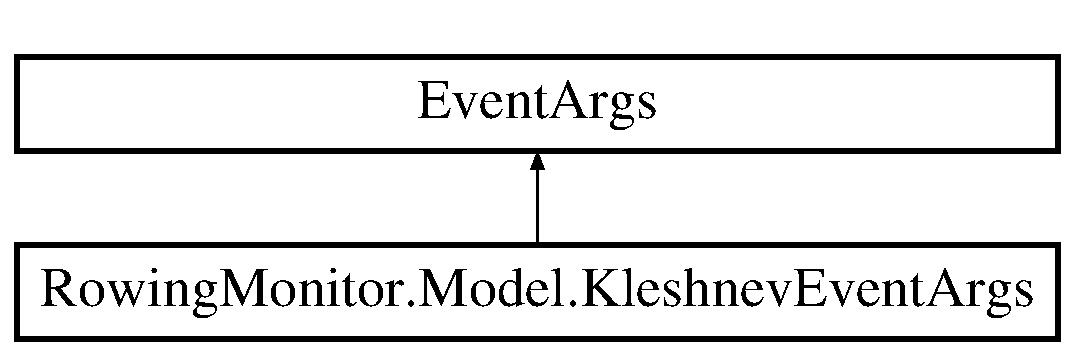
\includegraphics[height=2.000000cm]{class_rowing_monitor_1_1_model_1_1_kleshnev_event_args}
\end{center}
\end{figure}
\subsection*{Public Member Functions}
\begin{DoxyCompactItemize}
\item 
\hyperlink{class_rowing_monitor_1_1_model_1_1_kleshnev_event_args_ad371c1b70b890d6991665a29120fb554}{Kleshnev\+Event\+Args} (List$<$ \hyperlink{struct_rowing_monitor_1_1_model_1_1_pipeline_1_1_kleshnev_data}{Kleshnev\+Data} $>$ kleshnev\+Data)
\end{DoxyCompactItemize}


\subsection{Detailed Description}
Represents the arguments for a finished Kleshnev analysis. 



\subsection{Constructor \& Destructor Documentation}
\mbox{\Hypertarget{class_rowing_monitor_1_1_model_1_1_kleshnev_event_args_ad371c1b70b890d6991665a29120fb554}\label{class_rowing_monitor_1_1_model_1_1_kleshnev_event_args_ad371c1b70b890d6991665a29120fb554}} 
\index{Rowing\+Monitor\+::\+Model\+::\+Kleshnev\+Event\+Args@{Rowing\+Monitor\+::\+Model\+::\+Kleshnev\+Event\+Args}!Kleshnev\+Event\+Args@{Kleshnev\+Event\+Args}}
\index{Kleshnev\+Event\+Args@{Kleshnev\+Event\+Args}!Rowing\+Monitor\+::\+Model\+::\+Kleshnev\+Event\+Args@{Rowing\+Monitor\+::\+Model\+::\+Kleshnev\+Event\+Args}}
\subsubsection{\texorpdfstring{Kleshnev\+Event\+Args()}{KleshnevEventArgs()}}
{\footnotesize\ttfamily Rowing\+Monitor.\+Model.\+Kleshnev\+Event\+Args.\+Kleshnev\+Event\+Args (\begin{DoxyParamCaption}\item[{List$<$ \hyperlink{struct_rowing_monitor_1_1_model_1_1_pipeline_1_1_kleshnev_data}{Kleshnev\+Data} $>$}]{kleshnev\+Data }\end{DoxyParamCaption})}



The documentation for this class was generated from the following file\+:\begin{DoxyCompactItemize}
\item 
Model/\+Event\+Args/\hyperlink{_kleshnev_event_args_8cs}{Kleshnev\+Event\+Args.\+cs}\end{DoxyCompactItemize}

\hypertarget{class_rowing_monitor_1_1_model_1_1_pipeline_1_1_kleshnev_plot}{}\section{Rowing\+Monitor.\+Model.\+Pipeline.\+Kleshnev\+Plot Class Reference}
\label{class_rowing_monitor_1_1_model_1_1_pipeline_1_1_kleshnev_plot}\index{Rowing\+Monitor.\+Model.\+Pipeline.\+Kleshnev\+Plot@{Rowing\+Monitor.\+Model.\+Pipeline.\+Kleshnev\+Plot}}
\subsection*{Public Member Functions}
\begin{DoxyCompactItemize}
\item 
\hyperlink{class_rowing_monitor_1_1_model_1_1_pipeline_1_1_kleshnev_plot_a892c72567b10ca5cd3ef48b4ad9adb6e}{Kleshnev\+Plot} (float range=0.\+0f)
\begin{DoxyCompactList}\small\item\em Creates a new Kleshnev plot with a plot for the last complete segment and an realtime plot of the current Kleshnev velocities. \end{DoxyCompactList}\item 
void \hyperlink{class_rowing_monitor_1_1_model_1_1_pipeline_1_1_kleshnev_plot_a879f9fed320882b414bee01067dbe904}{Render} ()
\end{DoxyCompactItemize}
\subsection*{Properties}
\begin{DoxyCompactItemize}
\item 
float \hyperlink{class_rowing_monitor_1_1_model_1_1_pipeline_1_1_kleshnev_plot_a207085f1a6dc22991a7f8bf6a0452cb8}{Range}\hspace{0.3cm}{\ttfamily  \mbox{[}get, set\mbox{]}}
\item 
Action\+Block$<$ \hyperlink{struct_rowing_monitor_1_1_model_1_1_pipeline_1_1_kleshnev_data}{Kleshnev\+Data} $>$ \hyperlink{class_rowing_monitor_1_1_model_1_1_pipeline_1_1_kleshnev_plot_af3a6e1668ca2bd06362f6849dbd1dd3d}{Kleshnev\+Data\+Block}\hspace{0.3cm}{\ttfamily  \mbox{[}get, set\mbox{]}}
\item 
Action\+Block$<$ List$<$ \hyperlink{struct_rowing_monitor_1_1_model_1_1_util_1_1_segment_hit}{Segment\+Hit} $>$ $>$ \hyperlink{class_rowing_monitor_1_1_model_1_1_pipeline_1_1_kleshnev_plot_a59b2751dcbac682302c7dff7f404f8e0}{Plot\+Hits\+Block}\hspace{0.3cm}{\ttfamily  \mbox{[}get, set\mbox{]}}
\item 
\hyperlink{class_rowing_monitor_1_1_view_1_1_kleshnev_plot_view}{Kleshnev\+Plot\+View} \hyperlink{class_rowing_monitor_1_1_model_1_1_pipeline_1_1_kleshnev_plot_a154ed82243dd60d53794d7aa2eaed202}{View}\hspace{0.3cm}{\ttfamily  \mbox{[}get, set\mbox{]}}
\end{DoxyCompactItemize}


\subsection{Constructor \& Destructor Documentation}
\mbox{\Hypertarget{class_rowing_monitor_1_1_model_1_1_pipeline_1_1_kleshnev_plot_a892c72567b10ca5cd3ef48b4ad9adb6e}\label{class_rowing_monitor_1_1_model_1_1_pipeline_1_1_kleshnev_plot_a892c72567b10ca5cd3ef48b4ad9adb6e}} 
\index{Rowing\+Monitor\+::\+Model\+::\+Pipeline\+::\+Kleshnev\+Plot@{Rowing\+Monitor\+::\+Model\+::\+Pipeline\+::\+Kleshnev\+Plot}!Kleshnev\+Plot@{Kleshnev\+Plot}}
\index{Kleshnev\+Plot@{Kleshnev\+Plot}!Rowing\+Monitor\+::\+Model\+::\+Pipeline\+::\+Kleshnev\+Plot@{Rowing\+Monitor\+::\+Model\+::\+Pipeline\+::\+Kleshnev\+Plot}}
\subsubsection{\texorpdfstring{Kleshnev\+Plot()}{KleshnevPlot()}}
{\footnotesize\ttfamily Rowing\+Monitor.\+Model.\+Pipeline.\+Kleshnev\+Plot.\+Kleshnev\+Plot (\begin{DoxyParamCaption}\item[{float}]{range = {\ttfamily 0.0f} }\end{DoxyParamCaption})}



Creates a new Kleshnev plot with a plot for the last complete segment and an realtime plot of the current Kleshnev velocities. 


\begin{DoxyParams}{Parameters}
{\em range} & Sets the time range in seconds to display in the realtime plot.\\
\hline
\end{DoxyParams}


\subsection{Member Function Documentation}
\mbox{\Hypertarget{class_rowing_monitor_1_1_model_1_1_pipeline_1_1_kleshnev_plot_a879f9fed320882b414bee01067dbe904}\label{class_rowing_monitor_1_1_model_1_1_pipeline_1_1_kleshnev_plot_a879f9fed320882b414bee01067dbe904}} 
\index{Rowing\+Monitor\+::\+Model\+::\+Pipeline\+::\+Kleshnev\+Plot@{Rowing\+Monitor\+::\+Model\+::\+Pipeline\+::\+Kleshnev\+Plot}!Render@{Render}}
\index{Render@{Render}!Rowing\+Monitor\+::\+Model\+::\+Pipeline\+::\+Kleshnev\+Plot@{Rowing\+Monitor\+::\+Model\+::\+Pipeline\+::\+Kleshnev\+Plot}}
\subsubsection{\texorpdfstring{Render()}{Render()}}
{\footnotesize\ttfamily void Rowing\+Monitor.\+Model.\+Pipeline.\+Kleshnev\+Plot.\+Render (\begin{DoxyParamCaption}{ }\end{DoxyParamCaption})}



\subsection{Property Documentation}
\mbox{\Hypertarget{class_rowing_monitor_1_1_model_1_1_pipeline_1_1_kleshnev_plot_af3a6e1668ca2bd06362f6849dbd1dd3d}\label{class_rowing_monitor_1_1_model_1_1_pipeline_1_1_kleshnev_plot_af3a6e1668ca2bd06362f6849dbd1dd3d}} 
\index{Rowing\+Monitor\+::\+Model\+::\+Pipeline\+::\+Kleshnev\+Plot@{Rowing\+Monitor\+::\+Model\+::\+Pipeline\+::\+Kleshnev\+Plot}!Kleshnev\+Data\+Block@{Kleshnev\+Data\+Block}}
\index{Kleshnev\+Data\+Block@{Kleshnev\+Data\+Block}!Rowing\+Monitor\+::\+Model\+::\+Pipeline\+::\+Kleshnev\+Plot@{Rowing\+Monitor\+::\+Model\+::\+Pipeline\+::\+Kleshnev\+Plot}}
\subsubsection{\texorpdfstring{Kleshnev\+Data\+Block}{KleshnevDataBlock}}
{\footnotesize\ttfamily Action\+Block$<$\hyperlink{struct_rowing_monitor_1_1_model_1_1_pipeline_1_1_kleshnev_data}{Kleshnev\+Data}$>$ Rowing\+Monitor.\+Model.\+Pipeline.\+Kleshnev\+Plot.\+Kleshnev\+Data\+Block\hspace{0.3cm}{\ttfamily [get]}, {\ttfamily [set]}}

\mbox{\Hypertarget{class_rowing_monitor_1_1_model_1_1_pipeline_1_1_kleshnev_plot_a59b2751dcbac682302c7dff7f404f8e0}\label{class_rowing_monitor_1_1_model_1_1_pipeline_1_1_kleshnev_plot_a59b2751dcbac682302c7dff7f404f8e0}} 
\index{Rowing\+Monitor\+::\+Model\+::\+Pipeline\+::\+Kleshnev\+Plot@{Rowing\+Monitor\+::\+Model\+::\+Pipeline\+::\+Kleshnev\+Plot}!Plot\+Hits\+Block@{Plot\+Hits\+Block}}
\index{Plot\+Hits\+Block@{Plot\+Hits\+Block}!Rowing\+Monitor\+::\+Model\+::\+Pipeline\+::\+Kleshnev\+Plot@{Rowing\+Monitor\+::\+Model\+::\+Pipeline\+::\+Kleshnev\+Plot}}
\subsubsection{\texorpdfstring{Plot\+Hits\+Block}{PlotHitsBlock}}
{\footnotesize\ttfamily Action\+Block$<$List$<$\hyperlink{struct_rowing_monitor_1_1_model_1_1_util_1_1_segment_hit}{Segment\+Hit}$>$ $>$ Rowing\+Monitor.\+Model.\+Pipeline.\+Kleshnev\+Plot.\+Plot\+Hits\+Block\hspace{0.3cm}{\ttfamily [get]}, {\ttfamily [set]}}

\mbox{\Hypertarget{class_rowing_monitor_1_1_model_1_1_pipeline_1_1_kleshnev_plot_a207085f1a6dc22991a7f8bf6a0452cb8}\label{class_rowing_monitor_1_1_model_1_1_pipeline_1_1_kleshnev_plot_a207085f1a6dc22991a7f8bf6a0452cb8}} 
\index{Rowing\+Monitor\+::\+Model\+::\+Pipeline\+::\+Kleshnev\+Plot@{Rowing\+Monitor\+::\+Model\+::\+Pipeline\+::\+Kleshnev\+Plot}!Range@{Range}}
\index{Range@{Range}!Rowing\+Monitor\+::\+Model\+::\+Pipeline\+::\+Kleshnev\+Plot@{Rowing\+Monitor\+::\+Model\+::\+Pipeline\+::\+Kleshnev\+Plot}}
\subsubsection{\texorpdfstring{Range}{Range}}
{\footnotesize\ttfamily float Rowing\+Monitor.\+Model.\+Pipeline.\+Kleshnev\+Plot.\+Range\hspace{0.3cm}{\ttfamily [get]}, {\ttfamily [set]}}

\mbox{\Hypertarget{class_rowing_monitor_1_1_model_1_1_pipeline_1_1_kleshnev_plot_a154ed82243dd60d53794d7aa2eaed202}\label{class_rowing_monitor_1_1_model_1_1_pipeline_1_1_kleshnev_plot_a154ed82243dd60d53794d7aa2eaed202}} 
\index{Rowing\+Monitor\+::\+Model\+::\+Pipeline\+::\+Kleshnev\+Plot@{Rowing\+Monitor\+::\+Model\+::\+Pipeline\+::\+Kleshnev\+Plot}!View@{View}}
\index{View@{View}!Rowing\+Monitor\+::\+Model\+::\+Pipeline\+::\+Kleshnev\+Plot@{Rowing\+Monitor\+::\+Model\+::\+Pipeline\+::\+Kleshnev\+Plot}}
\subsubsection{\texorpdfstring{View}{View}}
{\footnotesize\ttfamily \hyperlink{class_rowing_monitor_1_1_view_1_1_kleshnev_plot_view}{Kleshnev\+Plot\+View} Rowing\+Monitor.\+Model.\+Pipeline.\+Kleshnev\+Plot.\+View\hspace{0.3cm}{\ttfamily [get]}, {\ttfamily [set]}}



The documentation for this class was generated from the following file\+:\begin{DoxyCompactItemize}
\item 
Model/\+Pipeline/\hyperlink{_kleshnev_plot_8cs}{Kleshnev\+Plot.\+cs}\end{DoxyCompactItemize}

\hypertarget{class_rowing_monitor_1_1_view_1_1_kleshnev_plot_view}{}\section{Rowing\+Monitor.\+View.\+Kleshnev\+Plot\+View Class Reference}
\label{class_rowing_monitor_1_1_view_1_1_kleshnev_plot_view}\index{Rowing\+Monitor.\+View.\+Kleshnev\+Plot\+View@{Rowing\+Monitor.\+View.\+Kleshnev\+Plot\+View}}


\hyperlink{class_rowing_monitor_1_1_view_1_1_kleshnev_plot_view}{Kleshnev\+Plot\+View}  


Inheritance diagram for Rowing\+Monitor.\+View.\+Kleshnev\+Plot\+View\+:\begin{figure}[H]
\begin{center}
\leavevmode
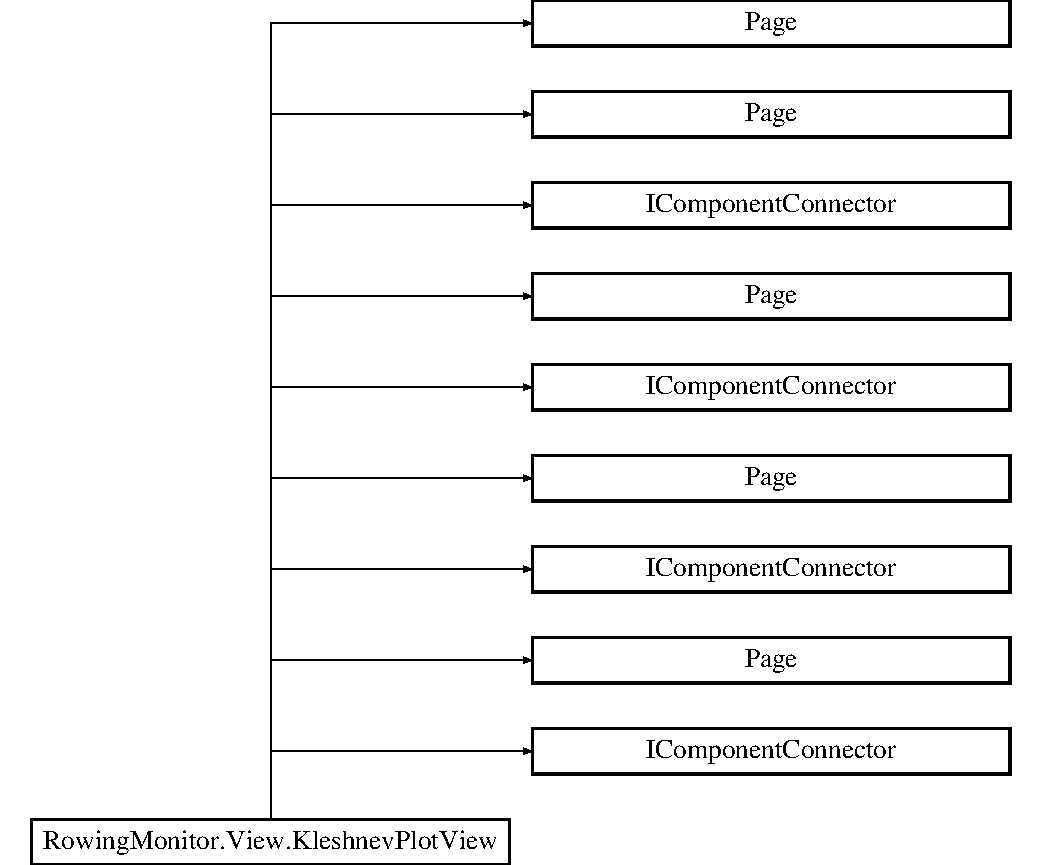
\includegraphics[height=10.000000cm]{class_rowing_monitor_1_1_view_1_1_kleshnev_plot_view}
\end{center}
\end{figure}
\subsection*{Public Member Functions}
\begin{DoxyCompactItemize}
\item 
void \hyperlink{class_rowing_monitor_1_1_view_1_1_kleshnev_plot_view_a378530c44bc7cb052db6f3a13cfc2db8}{Initialize\+Component} ()
\begin{DoxyCompactList}\small\item\em Initialize\+Component \end{DoxyCompactList}\item 
void \hyperlink{class_rowing_monitor_1_1_view_1_1_kleshnev_plot_view_a378530c44bc7cb052db6f3a13cfc2db8}{Initialize\+Component} ()
\begin{DoxyCompactList}\small\item\em Initialize\+Component \end{DoxyCompactList}\item 
void \hyperlink{class_rowing_monitor_1_1_view_1_1_kleshnev_plot_view_a378530c44bc7cb052db6f3a13cfc2db8}{Initialize\+Component} ()
\begin{DoxyCompactList}\small\item\em Initialize\+Component \end{DoxyCompactList}\item 
void \hyperlink{class_rowing_monitor_1_1_view_1_1_kleshnev_plot_view_a378530c44bc7cb052db6f3a13cfc2db8}{Initialize\+Component} ()
\begin{DoxyCompactList}\small\item\em Initialize\+Component \end{DoxyCompactList}\item 
\hyperlink{class_rowing_monitor_1_1_view_1_1_kleshnev_plot_view_a3e703e3daef530061957b5c15978ae56}{Kleshnev\+Plot\+View} ()
\end{DoxyCompactItemize}


\subsection{Detailed Description}
\hyperlink{class_rowing_monitor_1_1_view_1_1_kleshnev_plot_view}{Kleshnev\+Plot\+View} 

Interaktionslogik für Kleshnev\+Plot\+View.\+xaml 

\subsection{Constructor \& Destructor Documentation}
\mbox{\Hypertarget{class_rowing_monitor_1_1_view_1_1_kleshnev_plot_view_a3e703e3daef530061957b5c15978ae56}\label{class_rowing_monitor_1_1_view_1_1_kleshnev_plot_view_a3e703e3daef530061957b5c15978ae56}} 
\index{Rowing\+Monitor\+::\+View\+::\+Kleshnev\+Plot\+View@{Rowing\+Monitor\+::\+View\+::\+Kleshnev\+Plot\+View}!Kleshnev\+Plot\+View@{Kleshnev\+Plot\+View}}
\index{Kleshnev\+Plot\+View@{Kleshnev\+Plot\+View}!Rowing\+Monitor\+::\+View\+::\+Kleshnev\+Plot\+View@{Rowing\+Monitor\+::\+View\+::\+Kleshnev\+Plot\+View}}
\subsubsection{\texorpdfstring{Kleshnev\+Plot\+View()}{KleshnevPlotView()}}
{\footnotesize\ttfamily Rowing\+Monitor.\+View.\+Kleshnev\+Plot\+View.\+Kleshnev\+Plot\+View (\begin{DoxyParamCaption}{ }\end{DoxyParamCaption})}



\subsection{Member Function Documentation}
\mbox{\Hypertarget{class_rowing_monitor_1_1_view_1_1_kleshnev_plot_view_a378530c44bc7cb052db6f3a13cfc2db8}\label{class_rowing_monitor_1_1_view_1_1_kleshnev_plot_view_a378530c44bc7cb052db6f3a13cfc2db8}} 
\index{Rowing\+Monitor\+::\+View\+::\+Kleshnev\+Plot\+View@{Rowing\+Monitor\+::\+View\+::\+Kleshnev\+Plot\+View}!Initialize\+Component@{Initialize\+Component}}
\index{Initialize\+Component@{Initialize\+Component}!Rowing\+Monitor\+::\+View\+::\+Kleshnev\+Plot\+View@{Rowing\+Monitor\+::\+View\+::\+Kleshnev\+Plot\+View}}
\subsubsection{\texorpdfstring{Initialize\+Component()}{InitializeComponent()}\hspace{0.1cm}{\footnotesize\ttfamily [1/4]}}
{\footnotesize\ttfamily void Rowing\+Monitor.\+View.\+Kleshnev\+Plot\+View.\+Initialize\+Component (\begin{DoxyParamCaption}{ }\end{DoxyParamCaption})}



Initialize\+Component 

\mbox{\Hypertarget{class_rowing_monitor_1_1_view_1_1_kleshnev_plot_view_a378530c44bc7cb052db6f3a13cfc2db8}\label{class_rowing_monitor_1_1_view_1_1_kleshnev_plot_view_a378530c44bc7cb052db6f3a13cfc2db8}} 
\index{Rowing\+Monitor\+::\+View\+::\+Kleshnev\+Plot\+View@{Rowing\+Monitor\+::\+View\+::\+Kleshnev\+Plot\+View}!Initialize\+Component@{Initialize\+Component}}
\index{Initialize\+Component@{Initialize\+Component}!Rowing\+Monitor\+::\+View\+::\+Kleshnev\+Plot\+View@{Rowing\+Monitor\+::\+View\+::\+Kleshnev\+Plot\+View}}
\subsubsection{\texorpdfstring{Initialize\+Component()}{InitializeComponent()}\hspace{0.1cm}{\footnotesize\ttfamily [2/4]}}
{\footnotesize\ttfamily void Rowing\+Monitor.\+View.\+Kleshnev\+Plot\+View.\+Initialize\+Component (\begin{DoxyParamCaption}{ }\end{DoxyParamCaption})}



Initialize\+Component 

\mbox{\Hypertarget{class_rowing_monitor_1_1_view_1_1_kleshnev_plot_view_a378530c44bc7cb052db6f3a13cfc2db8}\label{class_rowing_monitor_1_1_view_1_1_kleshnev_plot_view_a378530c44bc7cb052db6f3a13cfc2db8}} 
\index{Rowing\+Monitor\+::\+View\+::\+Kleshnev\+Plot\+View@{Rowing\+Monitor\+::\+View\+::\+Kleshnev\+Plot\+View}!Initialize\+Component@{Initialize\+Component}}
\index{Initialize\+Component@{Initialize\+Component}!Rowing\+Monitor\+::\+View\+::\+Kleshnev\+Plot\+View@{Rowing\+Monitor\+::\+View\+::\+Kleshnev\+Plot\+View}}
\subsubsection{\texorpdfstring{Initialize\+Component()}{InitializeComponent()}\hspace{0.1cm}{\footnotesize\ttfamily [3/4]}}
{\footnotesize\ttfamily void Rowing\+Monitor.\+View.\+Kleshnev\+Plot\+View.\+Initialize\+Component (\begin{DoxyParamCaption}{ }\end{DoxyParamCaption})}



Initialize\+Component 

\mbox{\Hypertarget{class_rowing_monitor_1_1_view_1_1_kleshnev_plot_view_a378530c44bc7cb052db6f3a13cfc2db8}\label{class_rowing_monitor_1_1_view_1_1_kleshnev_plot_view_a378530c44bc7cb052db6f3a13cfc2db8}} 
\index{Rowing\+Monitor\+::\+View\+::\+Kleshnev\+Plot\+View@{Rowing\+Monitor\+::\+View\+::\+Kleshnev\+Plot\+View}!Initialize\+Component@{Initialize\+Component}}
\index{Initialize\+Component@{Initialize\+Component}!Rowing\+Monitor\+::\+View\+::\+Kleshnev\+Plot\+View@{Rowing\+Monitor\+::\+View\+::\+Kleshnev\+Plot\+View}}
\subsubsection{\texorpdfstring{Initialize\+Component()}{InitializeComponent()}\hspace{0.1cm}{\footnotesize\ttfamily [4/4]}}
{\footnotesize\ttfamily void Rowing\+Monitor.\+View.\+Kleshnev\+Plot\+View.\+Initialize\+Component (\begin{DoxyParamCaption}{ }\end{DoxyParamCaption})}



Initialize\+Component 



The documentation for this class was generated from the following files\+:\begin{DoxyCompactItemize}
\item 
obj/\+Debug/\+View/\hyperlink{_debug_2_view_2_kleshnev_plot_view_8g_8cs}{Kleshnev\+Plot\+View.\+g.\+cs}\item 
obj/\+Debug/\+View/\hyperlink{_debug_2_view_2_kleshnev_plot_view_8g_8i_8cs}{Kleshnev\+Plot\+View.\+g.\+i.\+cs}\item 
View/\hyperlink{_kleshnev_plot_view_8xaml_8cs}{Kleshnev\+Plot\+View.\+xaml.\+cs}\end{DoxyCompactItemize}

\hypertarget{class_rowing_monitor_1_1_view_model_1_1_kleshnev_plot_view_model}{}\section{Rowing\+Monitor.\+View\+Model.\+Kleshnev\+Plot\+View\+Model Class Reference}
\label{class_rowing_monitor_1_1_view_model_1_1_kleshnev_plot_view_model}\index{Rowing\+Monitor.\+View\+Model.\+Kleshnev\+Plot\+View\+Model@{Rowing\+Monitor.\+View\+Model.\+Kleshnev\+Plot\+View\+Model}}
Inheritance diagram for Rowing\+Monitor.\+View\+Model.\+Kleshnev\+Plot\+View\+Model\+:\begin{figure}[H]
\begin{center}
\leavevmode
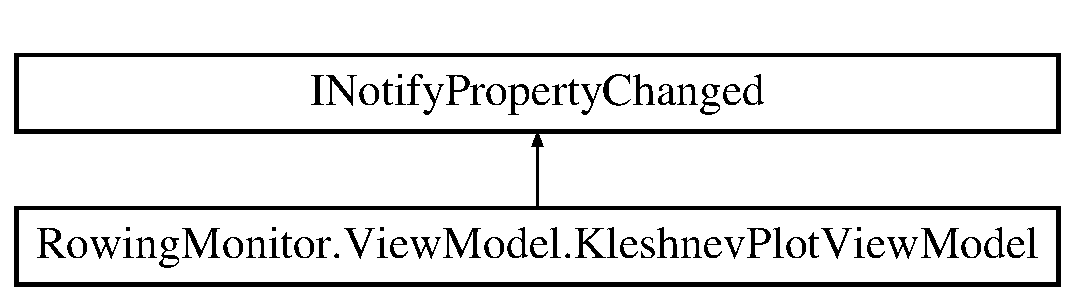
\includegraphics[height=2.000000cm]{class_rowing_monitor_1_1_view_model_1_1_kleshnev_plot_view_model}
\end{center}
\end{figure}
\subsection*{Public Member Functions}
\begin{DoxyCompactItemize}
\item 
\hyperlink{class_rowing_monitor_1_1_view_model_1_1_kleshnev_plot_view_model_a4389cc85cf8f9505fc14e8c9dac8ce36}{Kleshnev\+Plot\+View\+Model} ()
\item 
void \hyperlink{class_rowing_monitor_1_1_view_model_1_1_kleshnev_plot_view_model_ae9d5c76eadb7b4830a05757b0f1cedc3}{Render} ()
\item 
void \hyperlink{class_rowing_monitor_1_1_view_model_1_1_kleshnev_plot_view_model_abf17c79d9aa509a6e21b44ccfa47bc8c}{Update\+Last\+Segment\+Plot} (Plot\+Model last\+Segment\+Plot)
\item 
void \hyperlink{class_rowing_monitor_1_1_view_model_1_1_kleshnev_plot_view_model_a7d0c67c1ca826d8de7ff9093d19f9d72}{Update\+Current\+Segment\+Plot} (Plot\+Model current\+Segment\+Plot)
\end{DoxyCompactItemize}
\subsection*{Properties}
\begin{DoxyCompactItemize}
\item 
Plot\+Model \hyperlink{class_rowing_monitor_1_1_view_model_1_1_kleshnev_plot_view_model_af35d0a979c83141a6dc40e71df701ed2}{Last\+Segment\+Plot\+Model}\hspace{0.3cm}{\ttfamily  \mbox{[}get, set\mbox{]}}
\item 
Plot\+Model \hyperlink{class_rowing_monitor_1_1_view_model_1_1_kleshnev_plot_view_model_a7d8136280ae36f895edb930c7235da7b}{Current\+Segment\+Plot\+Model}\hspace{0.3cm}{\ttfamily  \mbox{[}get, set\mbox{]}}
\end{DoxyCompactItemize}
\subsection*{Events}
\begin{DoxyCompactItemize}
\item 
Property\+Changed\+Event\+Handler \hyperlink{class_rowing_monitor_1_1_view_model_1_1_kleshnev_plot_view_model_a6c7aa3954d98984a2b6c360a207af8aa}{Property\+Changed}
\end{DoxyCompactItemize}


\subsection{Constructor \& Destructor Documentation}
\mbox{\Hypertarget{class_rowing_monitor_1_1_view_model_1_1_kleshnev_plot_view_model_a4389cc85cf8f9505fc14e8c9dac8ce36}\label{class_rowing_monitor_1_1_view_model_1_1_kleshnev_plot_view_model_a4389cc85cf8f9505fc14e8c9dac8ce36}} 
\index{Rowing\+Monitor\+::\+View\+Model\+::\+Kleshnev\+Plot\+View\+Model@{Rowing\+Monitor\+::\+View\+Model\+::\+Kleshnev\+Plot\+View\+Model}!Kleshnev\+Plot\+View\+Model@{Kleshnev\+Plot\+View\+Model}}
\index{Kleshnev\+Plot\+View\+Model@{Kleshnev\+Plot\+View\+Model}!Rowing\+Monitor\+::\+View\+Model\+::\+Kleshnev\+Plot\+View\+Model@{Rowing\+Monitor\+::\+View\+Model\+::\+Kleshnev\+Plot\+View\+Model}}
\subsubsection{\texorpdfstring{Kleshnev\+Plot\+View\+Model()}{KleshnevPlotViewModel()}}
{\footnotesize\ttfamily Rowing\+Monitor.\+View\+Model.\+Kleshnev\+Plot\+View\+Model.\+Kleshnev\+Plot\+View\+Model (\begin{DoxyParamCaption}{ }\end{DoxyParamCaption})}



\subsection{Member Function Documentation}
\mbox{\Hypertarget{class_rowing_monitor_1_1_view_model_1_1_kleshnev_plot_view_model_ae9d5c76eadb7b4830a05757b0f1cedc3}\label{class_rowing_monitor_1_1_view_model_1_1_kleshnev_plot_view_model_ae9d5c76eadb7b4830a05757b0f1cedc3}} 
\index{Rowing\+Monitor\+::\+View\+Model\+::\+Kleshnev\+Plot\+View\+Model@{Rowing\+Monitor\+::\+View\+Model\+::\+Kleshnev\+Plot\+View\+Model}!Render@{Render}}
\index{Render@{Render}!Rowing\+Monitor\+::\+View\+Model\+::\+Kleshnev\+Plot\+View\+Model@{Rowing\+Monitor\+::\+View\+Model\+::\+Kleshnev\+Plot\+View\+Model}}
\subsubsection{\texorpdfstring{Render()}{Render()}}
{\footnotesize\ttfamily void Rowing\+Monitor.\+View\+Model.\+Kleshnev\+Plot\+View\+Model.\+Render (\begin{DoxyParamCaption}{ }\end{DoxyParamCaption})}

\mbox{\Hypertarget{class_rowing_monitor_1_1_view_model_1_1_kleshnev_plot_view_model_a7d0c67c1ca826d8de7ff9093d19f9d72}\label{class_rowing_monitor_1_1_view_model_1_1_kleshnev_plot_view_model_a7d0c67c1ca826d8de7ff9093d19f9d72}} 
\index{Rowing\+Monitor\+::\+View\+Model\+::\+Kleshnev\+Plot\+View\+Model@{Rowing\+Monitor\+::\+View\+Model\+::\+Kleshnev\+Plot\+View\+Model}!Update\+Current\+Segment\+Plot@{Update\+Current\+Segment\+Plot}}
\index{Update\+Current\+Segment\+Plot@{Update\+Current\+Segment\+Plot}!Rowing\+Monitor\+::\+View\+Model\+::\+Kleshnev\+Plot\+View\+Model@{Rowing\+Monitor\+::\+View\+Model\+::\+Kleshnev\+Plot\+View\+Model}}
\subsubsection{\texorpdfstring{Update\+Current\+Segment\+Plot()}{UpdateCurrentSegmentPlot()}}
{\footnotesize\ttfamily void Rowing\+Monitor.\+View\+Model.\+Kleshnev\+Plot\+View\+Model.\+Update\+Current\+Segment\+Plot (\begin{DoxyParamCaption}\item[{Plot\+Model}]{current\+Segment\+Plot }\end{DoxyParamCaption})}

\mbox{\Hypertarget{class_rowing_monitor_1_1_view_model_1_1_kleshnev_plot_view_model_abf17c79d9aa509a6e21b44ccfa47bc8c}\label{class_rowing_monitor_1_1_view_model_1_1_kleshnev_plot_view_model_abf17c79d9aa509a6e21b44ccfa47bc8c}} 
\index{Rowing\+Monitor\+::\+View\+Model\+::\+Kleshnev\+Plot\+View\+Model@{Rowing\+Monitor\+::\+View\+Model\+::\+Kleshnev\+Plot\+View\+Model}!Update\+Last\+Segment\+Plot@{Update\+Last\+Segment\+Plot}}
\index{Update\+Last\+Segment\+Plot@{Update\+Last\+Segment\+Plot}!Rowing\+Monitor\+::\+View\+Model\+::\+Kleshnev\+Plot\+View\+Model@{Rowing\+Monitor\+::\+View\+Model\+::\+Kleshnev\+Plot\+View\+Model}}
\subsubsection{\texorpdfstring{Update\+Last\+Segment\+Plot()}{UpdateLastSegmentPlot()}}
{\footnotesize\ttfamily void Rowing\+Monitor.\+View\+Model.\+Kleshnev\+Plot\+View\+Model.\+Update\+Last\+Segment\+Plot (\begin{DoxyParamCaption}\item[{Plot\+Model}]{last\+Segment\+Plot }\end{DoxyParamCaption})}



\subsection{Property Documentation}
\mbox{\Hypertarget{class_rowing_monitor_1_1_view_model_1_1_kleshnev_plot_view_model_a7d8136280ae36f895edb930c7235da7b}\label{class_rowing_monitor_1_1_view_model_1_1_kleshnev_plot_view_model_a7d8136280ae36f895edb930c7235da7b}} 
\index{Rowing\+Monitor\+::\+View\+Model\+::\+Kleshnev\+Plot\+View\+Model@{Rowing\+Monitor\+::\+View\+Model\+::\+Kleshnev\+Plot\+View\+Model}!Current\+Segment\+Plot\+Model@{Current\+Segment\+Plot\+Model}}
\index{Current\+Segment\+Plot\+Model@{Current\+Segment\+Plot\+Model}!Rowing\+Monitor\+::\+View\+Model\+::\+Kleshnev\+Plot\+View\+Model@{Rowing\+Monitor\+::\+View\+Model\+::\+Kleshnev\+Plot\+View\+Model}}
\subsubsection{\texorpdfstring{Current\+Segment\+Plot\+Model}{CurrentSegmentPlotModel}}
{\footnotesize\ttfamily Plot\+Model Rowing\+Monitor.\+View\+Model.\+Kleshnev\+Plot\+View\+Model.\+Current\+Segment\+Plot\+Model\hspace{0.3cm}{\ttfamily [get]}, {\ttfamily [set]}}

\mbox{\Hypertarget{class_rowing_monitor_1_1_view_model_1_1_kleshnev_plot_view_model_af35d0a979c83141a6dc40e71df701ed2}\label{class_rowing_monitor_1_1_view_model_1_1_kleshnev_plot_view_model_af35d0a979c83141a6dc40e71df701ed2}} 
\index{Rowing\+Monitor\+::\+View\+Model\+::\+Kleshnev\+Plot\+View\+Model@{Rowing\+Monitor\+::\+View\+Model\+::\+Kleshnev\+Plot\+View\+Model}!Last\+Segment\+Plot\+Model@{Last\+Segment\+Plot\+Model}}
\index{Last\+Segment\+Plot\+Model@{Last\+Segment\+Plot\+Model}!Rowing\+Monitor\+::\+View\+Model\+::\+Kleshnev\+Plot\+View\+Model@{Rowing\+Monitor\+::\+View\+Model\+::\+Kleshnev\+Plot\+View\+Model}}
\subsubsection{\texorpdfstring{Last\+Segment\+Plot\+Model}{LastSegmentPlotModel}}
{\footnotesize\ttfamily Plot\+Model Rowing\+Monitor.\+View\+Model.\+Kleshnev\+Plot\+View\+Model.\+Last\+Segment\+Plot\+Model\hspace{0.3cm}{\ttfamily [get]}, {\ttfamily [set]}}



\subsection{Event Documentation}
\mbox{\Hypertarget{class_rowing_monitor_1_1_view_model_1_1_kleshnev_plot_view_model_a6c7aa3954d98984a2b6c360a207af8aa}\label{class_rowing_monitor_1_1_view_model_1_1_kleshnev_plot_view_model_a6c7aa3954d98984a2b6c360a207af8aa}} 
\index{Rowing\+Monitor\+::\+View\+Model\+::\+Kleshnev\+Plot\+View\+Model@{Rowing\+Monitor\+::\+View\+Model\+::\+Kleshnev\+Plot\+View\+Model}!Property\+Changed@{Property\+Changed}}
\index{Property\+Changed@{Property\+Changed}!Rowing\+Monitor\+::\+View\+Model\+::\+Kleshnev\+Plot\+View\+Model@{Rowing\+Monitor\+::\+View\+Model\+::\+Kleshnev\+Plot\+View\+Model}}
\subsubsection{\texorpdfstring{Property\+Changed}{PropertyChanged}}
{\footnotesize\ttfamily Property\+Changed\+Event\+Handler Rowing\+Monitor.\+View\+Model.\+Kleshnev\+Plot\+View\+Model.\+Property\+Changed}



The documentation for this class was generated from the following file\+:\begin{DoxyCompactItemize}
\item 
View\+Model/\hyperlink{_kleshnev_plot_view_model_8cs}{Kleshnev\+Plot\+View\+Model.\+cs}\end{DoxyCompactItemize}

\hypertarget{class_rowing_monitor_1_1_model_1_1_pipeline_1_1_kleshnev_velocity_calculator}{}\section{Rowing\+Monitor.\+Model.\+Pipeline.\+Kleshnev\+Velocity\+Calculator Class Reference}
\label{class_rowing_monitor_1_1_model_1_1_pipeline_1_1_kleshnev_velocity_calculator}\index{Rowing\+Monitor.\+Model.\+Pipeline.\+Kleshnev\+Velocity\+Calculator@{Rowing\+Monitor.\+Model.\+Pipeline.\+Kleshnev\+Velocity\+Calculator}}
\subsection*{Public Member Functions}
\begin{DoxyCompactItemize}
\item 
delegate void \hyperlink{class_rowing_monitor_1_1_model_1_1_pipeline_1_1_kleshnev_velocity_calculator_aa8c251dc416d32f364bf138f4abeada7}{Kleshnev\+Calculation\+Finished\+Event\+Handler} (Object sender, \hyperlink{class_rowing_monitor_1_1_model_1_1_kleshnev_event_args}{Kleshnev\+Event\+Args} e)
\item 
\hyperlink{class_rowing_monitor_1_1_model_1_1_pipeline_1_1_kleshnev_velocity_calculator_ae642d137281c0ce38a84300066b28a64}{Kleshnev\+Velocity\+Calculator} ()
\item 
void \hyperlink{class_rowing_monitor_1_1_model_1_1_pipeline_1_1_kleshnev_velocity_calculator_af2ff2cb627827d1167732566636cc593}{Update} (\hyperlink{struct_rowing_monitor_1_1_model_1_1_util_1_1_joint_data}{Joint\+Data} joint\+Data)
\item 
List$<$ \hyperlink{struct_rowing_monitor_1_1_model_1_1_pipeline_1_1_kleshnev_data}{Kleshnev\+Data} $>$ \hyperlink{class_rowing_monitor_1_1_model_1_1_pipeline_1_1_kleshnev_velocity_calculator_a24776dfe3d1a8d3a499bfa48e721a868}{Calculate\+Kleshnev\+Velocities} (\hyperlink{struct_rowing_monitor_1_1_model_1_1_util_1_1_joint_data}{Joint\+Data} velocity\+Joint\+Data)
\end{DoxyCompactItemize}
\subsection*{Properties}
\begin{DoxyCompactItemize}
\item 
Broadcast\+Block$<$ \hyperlink{struct_rowing_monitor_1_1_model_1_1_pipeline_1_1_kleshnev_data}{Kleshnev\+Data} $>$ \hyperlink{class_rowing_monitor_1_1_model_1_1_pipeline_1_1_kleshnev_velocity_calculator_aed5495aa6d896a442ce39926ee30ed2c}{Output}\hspace{0.3cm}{\ttfamily  \mbox{[}get, set\mbox{]}}
\item 
Action\+Block$<$ \hyperlink{struct_rowing_monitor_1_1_model_1_1_util_1_1_joint_data}{Joint\+Data} $>$ \hyperlink{class_rowing_monitor_1_1_model_1_1_pipeline_1_1_kleshnev_velocity_calculator_a87c25ad950ba36047df4367a3a90cd20}{Input}\hspace{0.3cm}{\ttfamily  \mbox{[}get, set\mbox{]}}
\end{DoxyCompactItemize}
\subsection*{Events}
\begin{DoxyCompactItemize}
\item 
\hyperlink{class_rowing_monitor_1_1_model_1_1_pipeline_1_1_kleshnev_velocity_calculator_aa8c251dc416d32f364bf138f4abeada7}{Kleshnev\+Calculation\+Finished\+Event\+Handler} \hyperlink{class_rowing_monitor_1_1_model_1_1_pipeline_1_1_kleshnev_velocity_calculator_afc60a4e7b76e1bfd9c12b5aacda05a51}{Kleshnev\+Calculation\+Finished}
\end{DoxyCompactItemize}


\subsection{Constructor \& Destructor Documentation}
\mbox{\Hypertarget{class_rowing_monitor_1_1_model_1_1_pipeline_1_1_kleshnev_velocity_calculator_ae642d137281c0ce38a84300066b28a64}\label{class_rowing_monitor_1_1_model_1_1_pipeline_1_1_kleshnev_velocity_calculator_ae642d137281c0ce38a84300066b28a64}} 
\index{Rowing\+Monitor\+::\+Model\+::\+Pipeline\+::\+Kleshnev\+Velocity\+Calculator@{Rowing\+Monitor\+::\+Model\+::\+Pipeline\+::\+Kleshnev\+Velocity\+Calculator}!Kleshnev\+Velocity\+Calculator@{Kleshnev\+Velocity\+Calculator}}
\index{Kleshnev\+Velocity\+Calculator@{Kleshnev\+Velocity\+Calculator}!Rowing\+Monitor\+::\+Model\+::\+Pipeline\+::\+Kleshnev\+Velocity\+Calculator@{Rowing\+Monitor\+::\+Model\+::\+Pipeline\+::\+Kleshnev\+Velocity\+Calculator}}
\subsubsection{\texorpdfstring{Kleshnev\+Velocity\+Calculator()}{KleshnevVelocityCalculator()}}
{\footnotesize\ttfamily Rowing\+Monitor.\+Model.\+Pipeline.\+Kleshnev\+Velocity\+Calculator.\+Kleshnev\+Velocity\+Calculator (\begin{DoxyParamCaption}{ }\end{DoxyParamCaption})}



\subsection{Member Function Documentation}
\mbox{\Hypertarget{class_rowing_monitor_1_1_model_1_1_pipeline_1_1_kleshnev_velocity_calculator_a24776dfe3d1a8d3a499bfa48e721a868}\label{class_rowing_monitor_1_1_model_1_1_pipeline_1_1_kleshnev_velocity_calculator_a24776dfe3d1a8d3a499bfa48e721a868}} 
\index{Rowing\+Monitor\+::\+Model\+::\+Pipeline\+::\+Kleshnev\+Velocity\+Calculator@{Rowing\+Monitor\+::\+Model\+::\+Pipeline\+::\+Kleshnev\+Velocity\+Calculator}!Calculate\+Kleshnev\+Velocities@{Calculate\+Kleshnev\+Velocities}}
\index{Calculate\+Kleshnev\+Velocities@{Calculate\+Kleshnev\+Velocities}!Rowing\+Monitor\+::\+Model\+::\+Pipeline\+::\+Kleshnev\+Velocity\+Calculator@{Rowing\+Monitor\+::\+Model\+::\+Pipeline\+::\+Kleshnev\+Velocity\+Calculator}}
\subsubsection{\texorpdfstring{Calculate\+Kleshnev\+Velocities()}{CalculateKleshnevVelocities()}}
{\footnotesize\ttfamily List$<$\hyperlink{struct_rowing_monitor_1_1_model_1_1_pipeline_1_1_kleshnev_data}{Kleshnev\+Data}$>$ Rowing\+Monitor.\+Model.\+Pipeline.\+Kleshnev\+Velocity\+Calculator.\+Calculate\+Kleshnev\+Velocities (\begin{DoxyParamCaption}\item[{\hyperlink{struct_rowing_monitor_1_1_model_1_1_util_1_1_joint_data}{Joint\+Data}}]{velocity\+Joint\+Data }\end{DoxyParamCaption})}

\mbox{\Hypertarget{class_rowing_monitor_1_1_model_1_1_pipeline_1_1_kleshnev_velocity_calculator_aa8c251dc416d32f364bf138f4abeada7}\label{class_rowing_monitor_1_1_model_1_1_pipeline_1_1_kleshnev_velocity_calculator_aa8c251dc416d32f364bf138f4abeada7}} 
\index{Rowing\+Monitor\+::\+Model\+::\+Pipeline\+::\+Kleshnev\+Velocity\+Calculator@{Rowing\+Monitor\+::\+Model\+::\+Pipeline\+::\+Kleshnev\+Velocity\+Calculator}!Kleshnev\+Calculation\+Finished\+Event\+Handler@{Kleshnev\+Calculation\+Finished\+Event\+Handler}}
\index{Kleshnev\+Calculation\+Finished\+Event\+Handler@{Kleshnev\+Calculation\+Finished\+Event\+Handler}!Rowing\+Monitor\+::\+Model\+::\+Pipeline\+::\+Kleshnev\+Velocity\+Calculator@{Rowing\+Monitor\+::\+Model\+::\+Pipeline\+::\+Kleshnev\+Velocity\+Calculator}}
\subsubsection{\texorpdfstring{Kleshnev\+Calculation\+Finished\+Event\+Handler()}{KleshnevCalculationFinishedEventHandler()}}
{\footnotesize\ttfamily delegate void Rowing\+Monitor.\+Model.\+Pipeline.\+Kleshnev\+Velocity\+Calculator.\+Kleshnev\+Calculation\+Finished\+Event\+Handler (\begin{DoxyParamCaption}\item[{Object}]{sender,  }\item[{\hyperlink{class_rowing_monitor_1_1_model_1_1_kleshnev_event_args}{Kleshnev\+Event\+Args}}]{e }\end{DoxyParamCaption})}

\mbox{\Hypertarget{class_rowing_monitor_1_1_model_1_1_pipeline_1_1_kleshnev_velocity_calculator_af2ff2cb627827d1167732566636cc593}\label{class_rowing_monitor_1_1_model_1_1_pipeline_1_1_kleshnev_velocity_calculator_af2ff2cb627827d1167732566636cc593}} 
\index{Rowing\+Monitor\+::\+Model\+::\+Pipeline\+::\+Kleshnev\+Velocity\+Calculator@{Rowing\+Monitor\+::\+Model\+::\+Pipeline\+::\+Kleshnev\+Velocity\+Calculator}!Update@{Update}}
\index{Update@{Update}!Rowing\+Monitor\+::\+Model\+::\+Pipeline\+::\+Kleshnev\+Velocity\+Calculator@{Rowing\+Monitor\+::\+Model\+::\+Pipeline\+::\+Kleshnev\+Velocity\+Calculator}}
\subsubsection{\texorpdfstring{Update()}{Update()}}
{\footnotesize\ttfamily void Rowing\+Monitor.\+Model.\+Pipeline.\+Kleshnev\+Velocity\+Calculator.\+Update (\begin{DoxyParamCaption}\item[{\hyperlink{struct_rowing_monitor_1_1_model_1_1_util_1_1_joint_data}{Joint\+Data}}]{joint\+Data }\end{DoxyParamCaption})}



\subsection{Property Documentation}
\mbox{\Hypertarget{class_rowing_monitor_1_1_model_1_1_pipeline_1_1_kleshnev_velocity_calculator_a87c25ad950ba36047df4367a3a90cd20}\label{class_rowing_monitor_1_1_model_1_1_pipeline_1_1_kleshnev_velocity_calculator_a87c25ad950ba36047df4367a3a90cd20}} 
\index{Rowing\+Monitor\+::\+Model\+::\+Pipeline\+::\+Kleshnev\+Velocity\+Calculator@{Rowing\+Monitor\+::\+Model\+::\+Pipeline\+::\+Kleshnev\+Velocity\+Calculator}!Input@{Input}}
\index{Input@{Input}!Rowing\+Monitor\+::\+Model\+::\+Pipeline\+::\+Kleshnev\+Velocity\+Calculator@{Rowing\+Monitor\+::\+Model\+::\+Pipeline\+::\+Kleshnev\+Velocity\+Calculator}}
\subsubsection{\texorpdfstring{Input}{Input}}
{\footnotesize\ttfamily Action\+Block$<$\hyperlink{struct_rowing_monitor_1_1_model_1_1_util_1_1_joint_data}{Joint\+Data}$>$ Rowing\+Monitor.\+Model.\+Pipeline.\+Kleshnev\+Velocity\+Calculator.\+Input\hspace{0.3cm}{\ttfamily [get]}, {\ttfamily [set]}}

\mbox{\Hypertarget{class_rowing_monitor_1_1_model_1_1_pipeline_1_1_kleshnev_velocity_calculator_aed5495aa6d896a442ce39926ee30ed2c}\label{class_rowing_monitor_1_1_model_1_1_pipeline_1_1_kleshnev_velocity_calculator_aed5495aa6d896a442ce39926ee30ed2c}} 
\index{Rowing\+Monitor\+::\+Model\+::\+Pipeline\+::\+Kleshnev\+Velocity\+Calculator@{Rowing\+Monitor\+::\+Model\+::\+Pipeline\+::\+Kleshnev\+Velocity\+Calculator}!Output@{Output}}
\index{Output@{Output}!Rowing\+Monitor\+::\+Model\+::\+Pipeline\+::\+Kleshnev\+Velocity\+Calculator@{Rowing\+Monitor\+::\+Model\+::\+Pipeline\+::\+Kleshnev\+Velocity\+Calculator}}
\subsubsection{\texorpdfstring{Output}{Output}}
{\footnotesize\ttfamily Broadcast\+Block$<$\hyperlink{struct_rowing_monitor_1_1_model_1_1_pipeline_1_1_kleshnev_data}{Kleshnev\+Data}$>$ Rowing\+Monitor.\+Model.\+Pipeline.\+Kleshnev\+Velocity\+Calculator.\+Output\hspace{0.3cm}{\ttfamily [get]}, {\ttfamily [set]}}



\subsection{Event Documentation}
\mbox{\Hypertarget{class_rowing_monitor_1_1_model_1_1_pipeline_1_1_kleshnev_velocity_calculator_afc60a4e7b76e1bfd9c12b5aacda05a51}\label{class_rowing_monitor_1_1_model_1_1_pipeline_1_1_kleshnev_velocity_calculator_afc60a4e7b76e1bfd9c12b5aacda05a51}} 
\index{Rowing\+Monitor\+::\+Model\+::\+Pipeline\+::\+Kleshnev\+Velocity\+Calculator@{Rowing\+Monitor\+::\+Model\+::\+Pipeline\+::\+Kleshnev\+Velocity\+Calculator}!Kleshnev\+Calculation\+Finished@{Kleshnev\+Calculation\+Finished}}
\index{Kleshnev\+Calculation\+Finished@{Kleshnev\+Calculation\+Finished}!Rowing\+Monitor\+::\+Model\+::\+Pipeline\+::\+Kleshnev\+Velocity\+Calculator@{Rowing\+Monitor\+::\+Model\+::\+Pipeline\+::\+Kleshnev\+Velocity\+Calculator}}
\subsubsection{\texorpdfstring{Kleshnev\+Calculation\+Finished}{KleshnevCalculationFinished}}
{\footnotesize\ttfamily \hyperlink{class_rowing_monitor_1_1_model_1_1_pipeline_1_1_kleshnev_velocity_calculator_aa8c251dc416d32f364bf138f4abeada7}{Kleshnev\+Calculation\+Finished\+Event\+Handler} Rowing\+Monitor.\+Model.\+Pipeline.\+Kleshnev\+Velocity\+Calculator.\+Kleshnev\+Calculation\+Finished}



The documentation for this class was generated from the following file\+:\begin{DoxyCompactItemize}
\item 
Model/\+Pipeline/\hyperlink{_kleshnev_velocity_calculator_8cs}{Kleshnev\+Velocity\+Calculator.\+cs}\end{DoxyCompactItemize}

\hypertarget{class_rowing_monitor_1_1_model_1_1_util_1_1_logger}{}\section{Rowing\+Monitor.\+Model.\+Util.\+Logger Class Reference}
\label{class_rowing_monitor_1_1_model_1_1_util_1_1_logger}\index{Rowing\+Monitor.\+Model.\+Util.\+Logger@{Rowing\+Monitor.\+Model.\+Util.\+Logger}}
\subsection*{Static Public Member Functions}
\begin{DoxyCompactItemize}
\item 
static void \hyperlink{class_rowing_monitor_1_1_model_1_1_util_1_1_logger_aa64fcd49049d76a54281be04da4c0d5b}{Log\+Times} (List$<$ double $>$ times, string module, string additional\+Info)
\item 
static void \hyperlink{class_rowing_monitor_1_1_model_1_1_util_1_1_logger_a2e14f39dd12fdf95095720632e55b621}{Log\+Timestamps} (List$<$ double $>$ timestamps, string module, string additional\+Info)
\item 
static void \hyperlink{class_rowing_monitor_1_1_model_1_1_util_1_1_logger_a1b414168be6dbaa6947e29cef91ac47f}{Log} (string module, string message)
\end{DoxyCompactItemize}


\subsection{Member Function Documentation}
\mbox{\Hypertarget{class_rowing_monitor_1_1_model_1_1_util_1_1_logger_a1b414168be6dbaa6947e29cef91ac47f}\label{class_rowing_monitor_1_1_model_1_1_util_1_1_logger_a1b414168be6dbaa6947e29cef91ac47f}} 
\index{Rowing\+Monitor\+::\+Model\+::\+Util\+::\+Logger@{Rowing\+Monitor\+::\+Model\+::\+Util\+::\+Logger}!Log@{Log}}
\index{Log@{Log}!Rowing\+Monitor\+::\+Model\+::\+Util\+::\+Logger@{Rowing\+Monitor\+::\+Model\+::\+Util\+::\+Logger}}
\subsubsection{\texorpdfstring{Log()}{Log()}}
{\footnotesize\ttfamily static void Rowing\+Monitor.\+Model.\+Util.\+Logger.\+Log (\begin{DoxyParamCaption}\item[{string}]{module,  }\item[{string}]{message }\end{DoxyParamCaption})\hspace{0.3cm}{\ttfamily [static]}}

\mbox{\Hypertarget{class_rowing_monitor_1_1_model_1_1_util_1_1_logger_aa64fcd49049d76a54281be04da4c0d5b}\label{class_rowing_monitor_1_1_model_1_1_util_1_1_logger_aa64fcd49049d76a54281be04da4c0d5b}} 
\index{Rowing\+Monitor\+::\+Model\+::\+Util\+::\+Logger@{Rowing\+Monitor\+::\+Model\+::\+Util\+::\+Logger}!Log\+Times@{Log\+Times}}
\index{Log\+Times@{Log\+Times}!Rowing\+Monitor\+::\+Model\+::\+Util\+::\+Logger@{Rowing\+Monitor\+::\+Model\+::\+Util\+::\+Logger}}
\subsubsection{\texorpdfstring{Log\+Times()}{LogTimes()}}
{\footnotesize\ttfamily static void Rowing\+Monitor.\+Model.\+Util.\+Logger.\+Log\+Times (\begin{DoxyParamCaption}\item[{List$<$ double $>$}]{times,  }\item[{string}]{module,  }\item[{string}]{additional\+Info }\end{DoxyParamCaption})\hspace{0.3cm}{\ttfamily [static]}}

\mbox{\Hypertarget{class_rowing_monitor_1_1_model_1_1_util_1_1_logger_a2e14f39dd12fdf95095720632e55b621}\label{class_rowing_monitor_1_1_model_1_1_util_1_1_logger_a2e14f39dd12fdf95095720632e55b621}} 
\index{Rowing\+Monitor\+::\+Model\+::\+Util\+::\+Logger@{Rowing\+Monitor\+::\+Model\+::\+Util\+::\+Logger}!Log\+Timestamps@{Log\+Timestamps}}
\index{Log\+Timestamps@{Log\+Timestamps}!Rowing\+Monitor\+::\+Model\+::\+Util\+::\+Logger@{Rowing\+Monitor\+::\+Model\+::\+Util\+::\+Logger}}
\subsubsection{\texorpdfstring{Log\+Timestamps()}{LogTimestamps()}}
{\footnotesize\ttfamily static void Rowing\+Monitor.\+Model.\+Util.\+Logger.\+Log\+Timestamps (\begin{DoxyParamCaption}\item[{List$<$ double $>$}]{timestamps,  }\item[{string}]{module,  }\item[{string}]{additional\+Info }\end{DoxyParamCaption})\hspace{0.3cm}{\ttfamily [static]}}



The documentation for this class was generated from the following file\+:\begin{DoxyCompactItemize}
\item 
Model/\+Util/\hyperlink{_logger_8cs}{Logger.\+cs}\end{DoxyCompactItemize}

\hypertarget{class_rowing_monitor_1_1_model_1_1_low_pass_filter}{}\section{Rowing\+Monitor.\+Model.\+Low\+Pass\+Filter Class Reference}
\label{class_rowing_monitor_1_1_model_1_1_low_pass_filter}\index{Rowing\+Monitor.\+Model.\+Low\+Pass\+Filter@{Rowing\+Monitor.\+Model.\+Low\+Pass\+Filter}}
\subsection*{Public Member Functions}
\begin{DoxyCompactItemize}
\item 
\hyperlink{class_rowing_monitor_1_1_model_1_1_low_pass_filter_ae2409a1bea75885b3de02c300f46bb68}{Low\+Pass\+Filter} ()
\item 
Dictionary$<$ Joint\+Type, Joint $>$ \hyperlink{class_rowing_monitor_1_1_model_1_1_low_pass_filter_abd95054e31280d78ad6d0d4a5bd106ea}{Filter} (Dictionary$<$ Joint\+Type, Joint $>$ joints, Dictionary$<$ Joint\+Type, Dictionary$<$ String, Double $>$$>$ alpha)
\end{DoxyCompactItemize}
\subsection*{Properties}
\begin{DoxyCompactItemize}
\item 
Dictionary$<$ Joint\+Type, Joint $>$ \hyperlink{class_rowing_monitor_1_1_model_1_1_low_pass_filter_ab5c930d79699ed13c290b56a9d4501c6}{Hatxprev}\hspace{0.3cm}{\ttfamily  \mbox{[}get\mbox{]}}
\end{DoxyCompactItemize}


\subsection{Constructor \& Destructor Documentation}
\mbox{\Hypertarget{class_rowing_monitor_1_1_model_1_1_low_pass_filter_ae2409a1bea75885b3de02c300f46bb68}\label{class_rowing_monitor_1_1_model_1_1_low_pass_filter_ae2409a1bea75885b3de02c300f46bb68}} 
\index{Rowing\+Monitor\+::\+Model\+::\+Low\+Pass\+Filter@{Rowing\+Monitor\+::\+Model\+::\+Low\+Pass\+Filter}!Low\+Pass\+Filter@{Low\+Pass\+Filter}}
\index{Low\+Pass\+Filter@{Low\+Pass\+Filter}!Rowing\+Monitor\+::\+Model\+::\+Low\+Pass\+Filter@{Rowing\+Monitor\+::\+Model\+::\+Low\+Pass\+Filter}}
\subsubsection{\texorpdfstring{Low\+Pass\+Filter()}{LowPassFilter()}}
{\footnotesize\ttfamily Rowing\+Monitor.\+Model.\+Low\+Pass\+Filter.\+Low\+Pass\+Filter (\begin{DoxyParamCaption}{ }\end{DoxyParamCaption})}



\subsection{Member Function Documentation}
\mbox{\Hypertarget{class_rowing_monitor_1_1_model_1_1_low_pass_filter_abd95054e31280d78ad6d0d4a5bd106ea}\label{class_rowing_monitor_1_1_model_1_1_low_pass_filter_abd95054e31280d78ad6d0d4a5bd106ea}} 
\index{Rowing\+Monitor\+::\+Model\+::\+Low\+Pass\+Filter@{Rowing\+Monitor\+::\+Model\+::\+Low\+Pass\+Filter}!Filter@{Filter}}
\index{Filter@{Filter}!Rowing\+Monitor\+::\+Model\+::\+Low\+Pass\+Filter@{Rowing\+Monitor\+::\+Model\+::\+Low\+Pass\+Filter}}
\subsubsection{\texorpdfstring{Filter()}{Filter()}}
{\footnotesize\ttfamily Dictionary$<$Joint\+Type, Joint$>$ Rowing\+Monitor.\+Model.\+Low\+Pass\+Filter.\+Filter (\begin{DoxyParamCaption}\item[{Dictionary$<$ Joint\+Type, Joint $>$}]{joints,  }\item[{Dictionary$<$ Joint\+Type, Dictionary$<$ String, Double $>$$>$}]{alpha }\end{DoxyParamCaption})}



\subsection{Property Documentation}
\mbox{\Hypertarget{class_rowing_monitor_1_1_model_1_1_low_pass_filter_ab5c930d79699ed13c290b56a9d4501c6}\label{class_rowing_monitor_1_1_model_1_1_low_pass_filter_ab5c930d79699ed13c290b56a9d4501c6}} 
\index{Rowing\+Monitor\+::\+Model\+::\+Low\+Pass\+Filter@{Rowing\+Monitor\+::\+Model\+::\+Low\+Pass\+Filter}!Hatxprev@{Hatxprev}}
\index{Hatxprev@{Hatxprev}!Rowing\+Monitor\+::\+Model\+::\+Low\+Pass\+Filter@{Rowing\+Monitor\+::\+Model\+::\+Low\+Pass\+Filter}}
\subsubsection{\texorpdfstring{Hatxprev}{Hatxprev}}
{\footnotesize\ttfamily Dictionary$<$Joint\+Type, Joint$>$ Rowing\+Monitor.\+Model.\+Low\+Pass\+Filter.\+Hatxprev\hspace{0.3cm}{\ttfamily [get]}}



The documentation for this class was generated from the following file\+:\begin{DoxyCompactItemize}
\item 
Model/\+Util/\hyperlink{_low_pass_filter_8cs}{Low\+Pass\+Filter.\+cs}\end{DoxyCompactItemize}

\hypertarget{class_rowing_monitor_1_1_model_1_1_util_1_1_lowpass_filter}{}\section{Rowing\+Monitor.\+Model.\+Util.\+Lowpass\+Filter Class Reference}
\label{class_rowing_monitor_1_1_model_1_1_util_1_1_lowpass_filter}\index{Rowing\+Monitor.\+Model.\+Util.\+Lowpass\+Filter@{Rowing\+Monitor.\+Model.\+Util.\+Lowpass\+Filter}}
\subsection*{Public Member Functions}
\begin{DoxyCompactItemize}
\item 
\hyperlink{class_rowing_monitor_1_1_model_1_1_util_1_1_lowpass_filter_a258e84fac0e6e0ab6abdf72c4aec1c41}{Lowpass\+Filter} ()
\item 
double \hyperlink{class_rowing_monitor_1_1_model_1_1_util_1_1_lowpass_filter_a2a851f6f9830809a675e07110f58c745}{Last} ()
\item 
double \hyperlink{class_rowing_monitor_1_1_model_1_1_util_1_1_lowpass_filter_a68efc64ceb80ce939a693f4a4389c0c8}{Filter} (double x, double alpha)
\end{DoxyCompactItemize}
\subsection*{Protected Attributes}
\begin{DoxyCompactItemize}
\item 
bool \hyperlink{class_rowing_monitor_1_1_model_1_1_util_1_1_lowpass_filter_a8d81ed9b3a6d910cf22d7ef743bb6163}{first\+Time}
\item 
double \hyperlink{class_rowing_monitor_1_1_model_1_1_util_1_1_lowpass_filter_a4f370cfcfee67c57efb594b6b4b0562d}{hat\+X\+Prev}
\end{DoxyCompactItemize}


\subsection{Constructor \& Destructor Documentation}
\mbox{\Hypertarget{class_rowing_monitor_1_1_model_1_1_util_1_1_lowpass_filter_a258e84fac0e6e0ab6abdf72c4aec1c41}\label{class_rowing_monitor_1_1_model_1_1_util_1_1_lowpass_filter_a258e84fac0e6e0ab6abdf72c4aec1c41}} 
\index{Rowing\+Monitor\+::\+Model\+::\+Util\+::\+Lowpass\+Filter@{Rowing\+Monitor\+::\+Model\+::\+Util\+::\+Lowpass\+Filter}!Lowpass\+Filter@{Lowpass\+Filter}}
\index{Lowpass\+Filter@{Lowpass\+Filter}!Rowing\+Monitor\+::\+Model\+::\+Util\+::\+Lowpass\+Filter@{Rowing\+Monitor\+::\+Model\+::\+Util\+::\+Lowpass\+Filter}}
\subsubsection{\texorpdfstring{Lowpass\+Filter()}{LowpassFilter()}}
{\footnotesize\ttfamily Rowing\+Monitor.\+Model.\+Util.\+Lowpass\+Filter.\+Lowpass\+Filter (\begin{DoxyParamCaption}{ }\end{DoxyParamCaption})}



\subsection{Member Function Documentation}
\mbox{\Hypertarget{class_rowing_monitor_1_1_model_1_1_util_1_1_lowpass_filter_a68efc64ceb80ce939a693f4a4389c0c8}\label{class_rowing_monitor_1_1_model_1_1_util_1_1_lowpass_filter_a68efc64ceb80ce939a693f4a4389c0c8}} 
\index{Rowing\+Monitor\+::\+Model\+::\+Util\+::\+Lowpass\+Filter@{Rowing\+Monitor\+::\+Model\+::\+Util\+::\+Lowpass\+Filter}!Filter@{Filter}}
\index{Filter@{Filter}!Rowing\+Monitor\+::\+Model\+::\+Util\+::\+Lowpass\+Filter@{Rowing\+Monitor\+::\+Model\+::\+Util\+::\+Lowpass\+Filter}}
\subsubsection{\texorpdfstring{Filter()}{Filter()}}
{\footnotesize\ttfamily double Rowing\+Monitor.\+Model.\+Util.\+Lowpass\+Filter.\+Filter (\begin{DoxyParamCaption}\item[{double}]{x,  }\item[{double}]{alpha }\end{DoxyParamCaption})}

\mbox{\Hypertarget{class_rowing_monitor_1_1_model_1_1_util_1_1_lowpass_filter_a2a851f6f9830809a675e07110f58c745}\label{class_rowing_monitor_1_1_model_1_1_util_1_1_lowpass_filter_a2a851f6f9830809a675e07110f58c745}} 
\index{Rowing\+Monitor\+::\+Model\+::\+Util\+::\+Lowpass\+Filter@{Rowing\+Monitor\+::\+Model\+::\+Util\+::\+Lowpass\+Filter}!Last@{Last}}
\index{Last@{Last}!Rowing\+Monitor\+::\+Model\+::\+Util\+::\+Lowpass\+Filter@{Rowing\+Monitor\+::\+Model\+::\+Util\+::\+Lowpass\+Filter}}
\subsubsection{\texorpdfstring{Last()}{Last()}}
{\footnotesize\ttfamily double Rowing\+Monitor.\+Model.\+Util.\+Lowpass\+Filter.\+Last (\begin{DoxyParamCaption}{ }\end{DoxyParamCaption})}



\subsection{Member Data Documentation}
\mbox{\Hypertarget{class_rowing_monitor_1_1_model_1_1_util_1_1_lowpass_filter_a8d81ed9b3a6d910cf22d7ef743bb6163}\label{class_rowing_monitor_1_1_model_1_1_util_1_1_lowpass_filter_a8d81ed9b3a6d910cf22d7ef743bb6163}} 
\index{Rowing\+Monitor\+::\+Model\+::\+Util\+::\+Lowpass\+Filter@{Rowing\+Monitor\+::\+Model\+::\+Util\+::\+Lowpass\+Filter}!first\+Time@{first\+Time}}
\index{first\+Time@{first\+Time}!Rowing\+Monitor\+::\+Model\+::\+Util\+::\+Lowpass\+Filter@{Rowing\+Monitor\+::\+Model\+::\+Util\+::\+Lowpass\+Filter}}
\subsubsection{\texorpdfstring{first\+Time}{firstTime}}
{\footnotesize\ttfamily bool Rowing\+Monitor.\+Model.\+Util.\+Lowpass\+Filter.\+first\+Time\hspace{0.3cm}{\ttfamily [protected]}}

\mbox{\Hypertarget{class_rowing_monitor_1_1_model_1_1_util_1_1_lowpass_filter_a4f370cfcfee67c57efb594b6b4b0562d}\label{class_rowing_monitor_1_1_model_1_1_util_1_1_lowpass_filter_a4f370cfcfee67c57efb594b6b4b0562d}} 
\index{Rowing\+Monitor\+::\+Model\+::\+Util\+::\+Lowpass\+Filter@{Rowing\+Monitor\+::\+Model\+::\+Util\+::\+Lowpass\+Filter}!hat\+X\+Prev@{hat\+X\+Prev}}
\index{hat\+X\+Prev@{hat\+X\+Prev}!Rowing\+Monitor\+::\+Model\+::\+Util\+::\+Lowpass\+Filter@{Rowing\+Monitor\+::\+Model\+::\+Util\+::\+Lowpass\+Filter}}
\subsubsection{\texorpdfstring{hat\+X\+Prev}{hatXPrev}}
{\footnotesize\ttfamily double Rowing\+Monitor.\+Model.\+Util.\+Lowpass\+Filter.\+hat\+X\+Prev\hspace{0.3cm}{\ttfamily [protected]}}



The documentation for this class was generated from the following file\+:\begin{DoxyCompactItemize}
\item 
Model/\+Util/\hyperlink{_one_euro_filter_8cs}{One\+Euro\+Filter.\+cs}\end{DoxyCompactItemize}

\hypertarget{class_rowing_monitor_1_1_main_window}{}\section{Rowing\+Monitor.\+Main\+Window Class Reference}
\label{class_rowing_monitor_1_1_main_window}\index{Rowing\+Monitor.\+Main\+Window@{Rowing\+Monitor.\+Main\+Window}}


Interaktionslogik für Main\+Window.\+xaml  


Inheritance diagram for Rowing\+Monitor.\+Main\+Window\+:\begin{figure}[H]
\begin{center}
\leavevmode
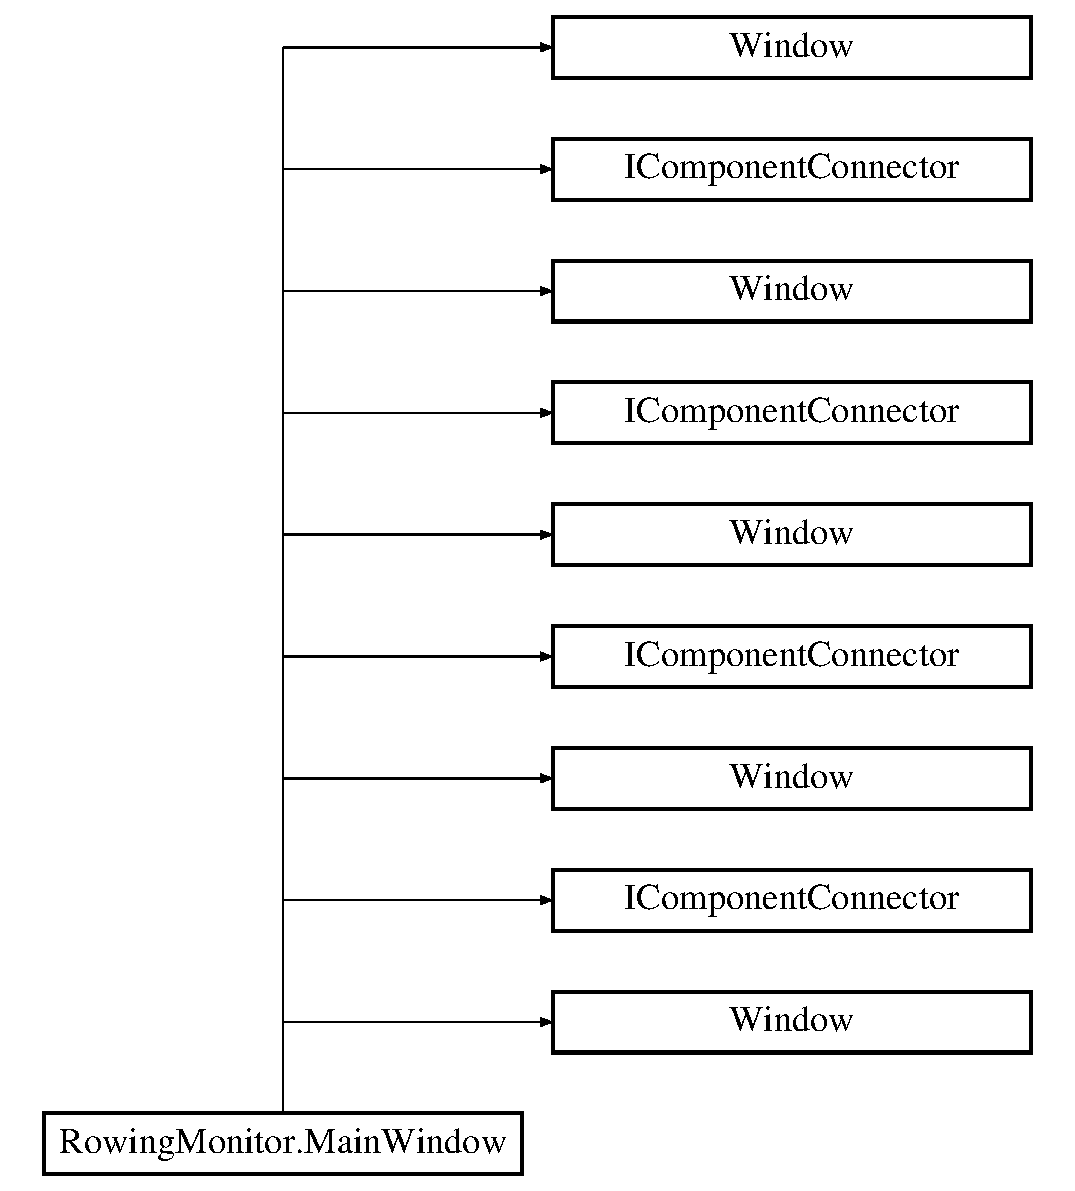
\includegraphics[height=9.000000cm]{class_rowing_monitor_1_1_main_window}
\end{center}
\end{figure}
\subsection*{Public Member Functions}
\begin{DoxyCompactItemize}
\item 
\hyperlink{class_rowing_monitor_1_1_main_window_aa33d7965b0fa09c32b1e7e2f782817d0}{Main\+Window} ()
\item 
void \hyperlink{class_rowing_monitor_1_1_main_window_afe76deea60e7fd9a534277f34037d22c}{Initialize\+Component} ()
\begin{DoxyCompactList}\small\item\em Initialize\+Component \end{DoxyCompactList}\item 
void \hyperlink{class_rowing_monitor_1_1_main_window_afe76deea60e7fd9a534277f34037d22c}{Initialize\+Component} ()
\begin{DoxyCompactList}\small\item\em Initialize\+Component \end{DoxyCompactList}\item 
void \hyperlink{class_rowing_monitor_1_1_main_window_afe76deea60e7fd9a534277f34037d22c}{Initialize\+Component} ()
\begin{DoxyCompactList}\small\item\em Initialize\+Component \end{DoxyCompactList}\item 
void \hyperlink{class_rowing_monitor_1_1_main_window_afe76deea60e7fd9a534277f34037d22c}{Initialize\+Component} ()
\begin{DoxyCompactList}\small\item\em Initialize\+Component \end{DoxyCompactList}\end{DoxyCompactItemize}


\subsection{Detailed Description}
Interaktionslogik für Main\+Window.\+xaml 

\hyperlink{class_rowing_monitor_1_1_main_window}{Main\+Window} 

\subsection{Constructor \& Destructor Documentation}
\mbox{\Hypertarget{class_rowing_monitor_1_1_main_window_aa33d7965b0fa09c32b1e7e2f782817d0}\label{class_rowing_monitor_1_1_main_window_aa33d7965b0fa09c32b1e7e2f782817d0}} 
\index{Rowing\+Monitor\+::\+Main\+Window@{Rowing\+Monitor\+::\+Main\+Window}!Main\+Window@{Main\+Window}}
\index{Main\+Window@{Main\+Window}!Rowing\+Monitor\+::\+Main\+Window@{Rowing\+Monitor\+::\+Main\+Window}}
\subsubsection{\texorpdfstring{Main\+Window()}{MainWindow()}}
{\footnotesize\ttfamily Rowing\+Monitor.\+Main\+Window.\+Main\+Window (\begin{DoxyParamCaption}{ }\end{DoxyParamCaption})}



\subsection{Member Function Documentation}
\mbox{\Hypertarget{class_rowing_monitor_1_1_main_window_afe76deea60e7fd9a534277f34037d22c}\label{class_rowing_monitor_1_1_main_window_afe76deea60e7fd9a534277f34037d22c}} 
\index{Rowing\+Monitor\+::\+Main\+Window@{Rowing\+Monitor\+::\+Main\+Window}!Initialize\+Component@{Initialize\+Component}}
\index{Initialize\+Component@{Initialize\+Component}!Rowing\+Monitor\+::\+Main\+Window@{Rowing\+Monitor\+::\+Main\+Window}}
\subsubsection{\texorpdfstring{Initialize\+Component()}{InitializeComponent()}\hspace{0.1cm}{\footnotesize\ttfamily [1/4]}}
{\footnotesize\ttfamily void Rowing\+Monitor.\+Main\+Window.\+Initialize\+Component (\begin{DoxyParamCaption}{ }\end{DoxyParamCaption})}



Initialize\+Component 

\mbox{\Hypertarget{class_rowing_monitor_1_1_main_window_afe76deea60e7fd9a534277f34037d22c}\label{class_rowing_monitor_1_1_main_window_afe76deea60e7fd9a534277f34037d22c}} 
\index{Rowing\+Monitor\+::\+Main\+Window@{Rowing\+Monitor\+::\+Main\+Window}!Initialize\+Component@{Initialize\+Component}}
\index{Initialize\+Component@{Initialize\+Component}!Rowing\+Monitor\+::\+Main\+Window@{Rowing\+Monitor\+::\+Main\+Window}}
\subsubsection{\texorpdfstring{Initialize\+Component()}{InitializeComponent()}\hspace{0.1cm}{\footnotesize\ttfamily [2/4]}}
{\footnotesize\ttfamily void Rowing\+Monitor.\+Main\+Window.\+Initialize\+Component (\begin{DoxyParamCaption}{ }\end{DoxyParamCaption})}



Initialize\+Component 

\mbox{\Hypertarget{class_rowing_monitor_1_1_main_window_afe76deea60e7fd9a534277f34037d22c}\label{class_rowing_monitor_1_1_main_window_afe76deea60e7fd9a534277f34037d22c}} 
\index{Rowing\+Monitor\+::\+Main\+Window@{Rowing\+Monitor\+::\+Main\+Window}!Initialize\+Component@{Initialize\+Component}}
\index{Initialize\+Component@{Initialize\+Component}!Rowing\+Monitor\+::\+Main\+Window@{Rowing\+Monitor\+::\+Main\+Window}}
\subsubsection{\texorpdfstring{Initialize\+Component()}{InitializeComponent()}\hspace{0.1cm}{\footnotesize\ttfamily [3/4]}}
{\footnotesize\ttfamily void Rowing\+Monitor.\+Main\+Window.\+Initialize\+Component (\begin{DoxyParamCaption}{ }\end{DoxyParamCaption})}



Initialize\+Component 

\mbox{\Hypertarget{class_rowing_monitor_1_1_main_window_afe76deea60e7fd9a534277f34037d22c}\label{class_rowing_monitor_1_1_main_window_afe76deea60e7fd9a534277f34037d22c}} 
\index{Rowing\+Monitor\+::\+Main\+Window@{Rowing\+Monitor\+::\+Main\+Window}!Initialize\+Component@{Initialize\+Component}}
\index{Initialize\+Component@{Initialize\+Component}!Rowing\+Monitor\+::\+Main\+Window@{Rowing\+Monitor\+::\+Main\+Window}}
\subsubsection{\texorpdfstring{Initialize\+Component()}{InitializeComponent()}\hspace{0.1cm}{\footnotesize\ttfamily [4/4]}}
{\footnotesize\ttfamily void Rowing\+Monitor.\+Main\+Window.\+Initialize\+Component (\begin{DoxyParamCaption}{ }\end{DoxyParamCaption})}



Initialize\+Component 



The documentation for this class was generated from the following files\+:\begin{DoxyCompactItemize}
\item 
\hyperlink{_main_window_8xaml_8cs}{Main\+Window.\+xaml.\+cs}\item 
obj/\+Debug/\hyperlink{_debug_2_main_window_8g_8cs}{Main\+Window.\+g.\+cs}\item 
obj/\+Debug/\hyperlink{_debug_2_main_window_8g_8i_8cs}{Main\+Window.\+g.\+i.\+cs}\end{DoxyCompactItemize}

\hypertarget{class_rowing_monitor_1_1_model_1_1_util_1_1_one_euro_filter}{}\section{Rowing\+Monitor.\+Model.\+Util.\+One\+Euro\+Filter Class Reference}
\label{class_rowing_monitor_1_1_model_1_1_util_1_1_one_euro_filter}\index{Rowing\+Monitor.\+Model.\+Util.\+One\+Euro\+Filter@{Rowing\+Monitor.\+Model.\+Util.\+One\+Euro\+Filter}}
\subsection*{Public Member Functions}
\begin{DoxyCompactItemize}
\item 
\hyperlink{class_rowing_monitor_1_1_model_1_1_util_1_1_one_euro_filter_a945b190ec38aa5a4fd9d440800becda5}{One\+Euro\+Filter} (double \hyperlink{class_rowing_monitor_1_1_model_1_1_util_1_1_one_euro_filter_a54c70fc75d1de35642fc30ef4ef78782}{min\+Cutoff}, double \hyperlink{class_rowing_monitor_1_1_model_1_1_util_1_1_one_euro_filter_a11b6badcd4065baa9453aa4672300fb3}{beta})
\item 
double \hyperlink{class_rowing_monitor_1_1_model_1_1_util_1_1_one_euro_filter_a4c0409d8b95c07c2b6dd4567fb438532}{Filter} (double x, double rate)
\end{DoxyCompactItemize}
\subsection*{Protected Member Functions}
\begin{DoxyCompactItemize}
\item 
double \hyperlink{class_rowing_monitor_1_1_model_1_1_util_1_1_one_euro_filter_abc822a48fcbff3daad7bbf5b9d056c8e}{Alpha} (double rate, double cutoff)
\end{DoxyCompactItemize}
\subsection*{Protected Attributes}
\begin{DoxyCompactItemize}
\item 
bool \hyperlink{class_rowing_monitor_1_1_model_1_1_util_1_1_one_euro_filter_aef4128061f9e58498c536a2f0238fb5e}{first\+Time}
\item 
double \hyperlink{class_rowing_monitor_1_1_model_1_1_util_1_1_one_euro_filter_a54c70fc75d1de35642fc30ef4ef78782}{min\+Cutoff}
\item 
double \hyperlink{class_rowing_monitor_1_1_model_1_1_util_1_1_one_euro_filter_a11b6badcd4065baa9453aa4672300fb3}{beta}
\item 
\hyperlink{class_rowing_monitor_1_1_model_1_1_util_1_1_lowpass_filter}{Lowpass\+Filter} \hyperlink{class_rowing_monitor_1_1_model_1_1_util_1_1_one_euro_filter_a8c5c8ede133408fde40a26fd11f0e9c0}{x\+Filt}
\item 
\hyperlink{class_rowing_monitor_1_1_model_1_1_util_1_1_lowpass_filter}{Lowpass\+Filter} \hyperlink{class_rowing_monitor_1_1_model_1_1_util_1_1_one_euro_filter_ab825015c12eda6bdbe6deaaa69ea44da}{dx\+Filt}
\item 
double \hyperlink{class_rowing_monitor_1_1_model_1_1_util_1_1_one_euro_filter_a6856ece1fd3069d3fda984a17be3f2f4}{dcutoff}
\end{DoxyCompactItemize}
\subsection*{Properties}
\begin{DoxyCompactItemize}
\item 
double \hyperlink{class_rowing_monitor_1_1_model_1_1_util_1_1_one_euro_filter_a65d1767883d487c73e340389d066f097}{Min\+Cutoff}\hspace{0.3cm}{\ttfamily  \mbox{[}get, set\mbox{]}}
\item 
double \hyperlink{class_rowing_monitor_1_1_model_1_1_util_1_1_one_euro_filter_a16e8bfe237364453b4ed8d79d05ba662}{Beta}\hspace{0.3cm}{\ttfamily  \mbox{[}get, set\mbox{]}}
\end{DoxyCompactItemize}


\subsection{Constructor \& Destructor Documentation}
\mbox{\Hypertarget{class_rowing_monitor_1_1_model_1_1_util_1_1_one_euro_filter_a945b190ec38aa5a4fd9d440800becda5}\label{class_rowing_monitor_1_1_model_1_1_util_1_1_one_euro_filter_a945b190ec38aa5a4fd9d440800becda5}} 
\index{Rowing\+Monitor\+::\+Model\+::\+Util\+::\+One\+Euro\+Filter@{Rowing\+Monitor\+::\+Model\+::\+Util\+::\+One\+Euro\+Filter}!One\+Euro\+Filter@{One\+Euro\+Filter}}
\index{One\+Euro\+Filter@{One\+Euro\+Filter}!Rowing\+Monitor\+::\+Model\+::\+Util\+::\+One\+Euro\+Filter@{Rowing\+Monitor\+::\+Model\+::\+Util\+::\+One\+Euro\+Filter}}
\subsubsection{\texorpdfstring{One\+Euro\+Filter()}{OneEuroFilter()}}
{\footnotesize\ttfamily Rowing\+Monitor.\+Model.\+Util.\+One\+Euro\+Filter.\+One\+Euro\+Filter (\begin{DoxyParamCaption}\item[{double}]{min\+Cutoff,  }\item[{double}]{beta }\end{DoxyParamCaption})}



\subsection{Member Function Documentation}
\mbox{\Hypertarget{class_rowing_monitor_1_1_model_1_1_util_1_1_one_euro_filter_abc822a48fcbff3daad7bbf5b9d056c8e}\label{class_rowing_monitor_1_1_model_1_1_util_1_1_one_euro_filter_abc822a48fcbff3daad7bbf5b9d056c8e}} 
\index{Rowing\+Monitor\+::\+Model\+::\+Util\+::\+One\+Euro\+Filter@{Rowing\+Monitor\+::\+Model\+::\+Util\+::\+One\+Euro\+Filter}!Alpha@{Alpha}}
\index{Alpha@{Alpha}!Rowing\+Monitor\+::\+Model\+::\+Util\+::\+One\+Euro\+Filter@{Rowing\+Monitor\+::\+Model\+::\+Util\+::\+One\+Euro\+Filter}}
\subsubsection{\texorpdfstring{Alpha()}{Alpha()}}
{\footnotesize\ttfamily double Rowing\+Monitor.\+Model.\+Util.\+One\+Euro\+Filter.\+Alpha (\begin{DoxyParamCaption}\item[{double}]{rate,  }\item[{double}]{cutoff }\end{DoxyParamCaption})\hspace{0.3cm}{\ttfamily [protected]}}

\mbox{\Hypertarget{class_rowing_monitor_1_1_model_1_1_util_1_1_one_euro_filter_a4c0409d8b95c07c2b6dd4567fb438532}\label{class_rowing_monitor_1_1_model_1_1_util_1_1_one_euro_filter_a4c0409d8b95c07c2b6dd4567fb438532}} 
\index{Rowing\+Monitor\+::\+Model\+::\+Util\+::\+One\+Euro\+Filter@{Rowing\+Monitor\+::\+Model\+::\+Util\+::\+One\+Euro\+Filter}!Filter@{Filter}}
\index{Filter@{Filter}!Rowing\+Monitor\+::\+Model\+::\+Util\+::\+One\+Euro\+Filter@{Rowing\+Monitor\+::\+Model\+::\+Util\+::\+One\+Euro\+Filter}}
\subsubsection{\texorpdfstring{Filter()}{Filter()}}
{\footnotesize\ttfamily double Rowing\+Monitor.\+Model.\+Util.\+One\+Euro\+Filter.\+Filter (\begin{DoxyParamCaption}\item[{double}]{x,  }\item[{double}]{rate }\end{DoxyParamCaption})}



\subsection{Member Data Documentation}
\mbox{\Hypertarget{class_rowing_monitor_1_1_model_1_1_util_1_1_one_euro_filter_a11b6badcd4065baa9453aa4672300fb3}\label{class_rowing_monitor_1_1_model_1_1_util_1_1_one_euro_filter_a11b6badcd4065baa9453aa4672300fb3}} 
\index{Rowing\+Monitor\+::\+Model\+::\+Util\+::\+One\+Euro\+Filter@{Rowing\+Monitor\+::\+Model\+::\+Util\+::\+One\+Euro\+Filter}!beta@{beta}}
\index{beta@{beta}!Rowing\+Monitor\+::\+Model\+::\+Util\+::\+One\+Euro\+Filter@{Rowing\+Monitor\+::\+Model\+::\+Util\+::\+One\+Euro\+Filter}}
\subsubsection{\texorpdfstring{beta}{beta}}
{\footnotesize\ttfamily double Rowing\+Monitor.\+Model.\+Util.\+One\+Euro\+Filter.\+beta\hspace{0.3cm}{\ttfamily [protected]}}

\mbox{\Hypertarget{class_rowing_monitor_1_1_model_1_1_util_1_1_one_euro_filter_a6856ece1fd3069d3fda984a17be3f2f4}\label{class_rowing_monitor_1_1_model_1_1_util_1_1_one_euro_filter_a6856ece1fd3069d3fda984a17be3f2f4}} 
\index{Rowing\+Monitor\+::\+Model\+::\+Util\+::\+One\+Euro\+Filter@{Rowing\+Monitor\+::\+Model\+::\+Util\+::\+One\+Euro\+Filter}!dcutoff@{dcutoff}}
\index{dcutoff@{dcutoff}!Rowing\+Monitor\+::\+Model\+::\+Util\+::\+One\+Euro\+Filter@{Rowing\+Monitor\+::\+Model\+::\+Util\+::\+One\+Euro\+Filter}}
\subsubsection{\texorpdfstring{dcutoff}{dcutoff}}
{\footnotesize\ttfamily double Rowing\+Monitor.\+Model.\+Util.\+One\+Euro\+Filter.\+dcutoff\hspace{0.3cm}{\ttfamily [protected]}}

\mbox{\Hypertarget{class_rowing_monitor_1_1_model_1_1_util_1_1_one_euro_filter_ab825015c12eda6bdbe6deaaa69ea44da}\label{class_rowing_monitor_1_1_model_1_1_util_1_1_one_euro_filter_ab825015c12eda6bdbe6deaaa69ea44da}} 
\index{Rowing\+Monitor\+::\+Model\+::\+Util\+::\+One\+Euro\+Filter@{Rowing\+Monitor\+::\+Model\+::\+Util\+::\+One\+Euro\+Filter}!dx\+Filt@{dx\+Filt}}
\index{dx\+Filt@{dx\+Filt}!Rowing\+Monitor\+::\+Model\+::\+Util\+::\+One\+Euro\+Filter@{Rowing\+Monitor\+::\+Model\+::\+Util\+::\+One\+Euro\+Filter}}
\subsubsection{\texorpdfstring{dx\+Filt}{dxFilt}}
{\footnotesize\ttfamily \hyperlink{class_rowing_monitor_1_1_model_1_1_util_1_1_lowpass_filter}{Lowpass\+Filter} Rowing\+Monitor.\+Model.\+Util.\+One\+Euro\+Filter.\+dx\+Filt\hspace{0.3cm}{\ttfamily [protected]}}

\mbox{\Hypertarget{class_rowing_monitor_1_1_model_1_1_util_1_1_one_euro_filter_aef4128061f9e58498c536a2f0238fb5e}\label{class_rowing_monitor_1_1_model_1_1_util_1_1_one_euro_filter_aef4128061f9e58498c536a2f0238fb5e}} 
\index{Rowing\+Monitor\+::\+Model\+::\+Util\+::\+One\+Euro\+Filter@{Rowing\+Monitor\+::\+Model\+::\+Util\+::\+One\+Euro\+Filter}!first\+Time@{first\+Time}}
\index{first\+Time@{first\+Time}!Rowing\+Monitor\+::\+Model\+::\+Util\+::\+One\+Euro\+Filter@{Rowing\+Monitor\+::\+Model\+::\+Util\+::\+One\+Euro\+Filter}}
\subsubsection{\texorpdfstring{first\+Time}{firstTime}}
{\footnotesize\ttfamily bool Rowing\+Monitor.\+Model.\+Util.\+One\+Euro\+Filter.\+first\+Time\hspace{0.3cm}{\ttfamily [protected]}}

\mbox{\Hypertarget{class_rowing_monitor_1_1_model_1_1_util_1_1_one_euro_filter_a54c70fc75d1de35642fc30ef4ef78782}\label{class_rowing_monitor_1_1_model_1_1_util_1_1_one_euro_filter_a54c70fc75d1de35642fc30ef4ef78782}} 
\index{Rowing\+Monitor\+::\+Model\+::\+Util\+::\+One\+Euro\+Filter@{Rowing\+Monitor\+::\+Model\+::\+Util\+::\+One\+Euro\+Filter}!min\+Cutoff@{min\+Cutoff}}
\index{min\+Cutoff@{min\+Cutoff}!Rowing\+Monitor\+::\+Model\+::\+Util\+::\+One\+Euro\+Filter@{Rowing\+Monitor\+::\+Model\+::\+Util\+::\+One\+Euro\+Filter}}
\subsubsection{\texorpdfstring{min\+Cutoff}{minCutoff}}
{\footnotesize\ttfamily double Rowing\+Monitor.\+Model.\+Util.\+One\+Euro\+Filter.\+min\+Cutoff\hspace{0.3cm}{\ttfamily [protected]}}

\mbox{\Hypertarget{class_rowing_monitor_1_1_model_1_1_util_1_1_one_euro_filter_a8c5c8ede133408fde40a26fd11f0e9c0}\label{class_rowing_monitor_1_1_model_1_1_util_1_1_one_euro_filter_a8c5c8ede133408fde40a26fd11f0e9c0}} 
\index{Rowing\+Monitor\+::\+Model\+::\+Util\+::\+One\+Euro\+Filter@{Rowing\+Monitor\+::\+Model\+::\+Util\+::\+One\+Euro\+Filter}!x\+Filt@{x\+Filt}}
\index{x\+Filt@{x\+Filt}!Rowing\+Monitor\+::\+Model\+::\+Util\+::\+One\+Euro\+Filter@{Rowing\+Monitor\+::\+Model\+::\+Util\+::\+One\+Euro\+Filter}}
\subsubsection{\texorpdfstring{x\+Filt}{xFilt}}
{\footnotesize\ttfamily \hyperlink{class_rowing_monitor_1_1_model_1_1_util_1_1_lowpass_filter}{Lowpass\+Filter} Rowing\+Monitor.\+Model.\+Util.\+One\+Euro\+Filter.\+x\+Filt\hspace{0.3cm}{\ttfamily [protected]}}



\subsection{Property Documentation}
\mbox{\Hypertarget{class_rowing_monitor_1_1_model_1_1_util_1_1_one_euro_filter_a16e8bfe237364453b4ed8d79d05ba662}\label{class_rowing_monitor_1_1_model_1_1_util_1_1_one_euro_filter_a16e8bfe237364453b4ed8d79d05ba662}} 
\index{Rowing\+Monitor\+::\+Model\+::\+Util\+::\+One\+Euro\+Filter@{Rowing\+Monitor\+::\+Model\+::\+Util\+::\+One\+Euro\+Filter}!Beta@{Beta}}
\index{Beta@{Beta}!Rowing\+Monitor\+::\+Model\+::\+Util\+::\+One\+Euro\+Filter@{Rowing\+Monitor\+::\+Model\+::\+Util\+::\+One\+Euro\+Filter}}
\subsubsection{\texorpdfstring{Beta}{Beta}}
{\footnotesize\ttfamily double Rowing\+Monitor.\+Model.\+Util.\+One\+Euro\+Filter.\+Beta\hspace{0.3cm}{\ttfamily [get]}, {\ttfamily [set]}}

\mbox{\Hypertarget{class_rowing_monitor_1_1_model_1_1_util_1_1_one_euro_filter_a65d1767883d487c73e340389d066f097}\label{class_rowing_monitor_1_1_model_1_1_util_1_1_one_euro_filter_a65d1767883d487c73e340389d066f097}} 
\index{Rowing\+Monitor\+::\+Model\+::\+Util\+::\+One\+Euro\+Filter@{Rowing\+Monitor\+::\+Model\+::\+Util\+::\+One\+Euro\+Filter}!Min\+Cutoff@{Min\+Cutoff}}
\index{Min\+Cutoff@{Min\+Cutoff}!Rowing\+Monitor\+::\+Model\+::\+Util\+::\+One\+Euro\+Filter@{Rowing\+Monitor\+::\+Model\+::\+Util\+::\+One\+Euro\+Filter}}
\subsubsection{\texorpdfstring{Min\+Cutoff}{MinCutoff}}
{\footnotesize\ttfamily double Rowing\+Monitor.\+Model.\+Util.\+One\+Euro\+Filter.\+Min\+Cutoff\hspace{0.3cm}{\ttfamily [get]}, {\ttfamily [set]}}



The documentation for this class was generated from the following file\+:\begin{DoxyCompactItemize}
\item 
Model/\+Util/\hyperlink{_one_euro_filter_8cs}{One\+Euro\+Filter.\+cs}\end{DoxyCompactItemize}

\hypertarget{class_rowing_monitor_1_1_model_1_1_pipeline_1_1_one_euro_smoothing_filter}{}\section{Rowing\+Monitor.\+Model.\+Pipeline.\+One\+Euro\+Smoothing\+Filter Class Reference}
\label{class_rowing_monitor_1_1_model_1_1_pipeline_1_1_one_euro_smoothing_filter}\index{Rowing\+Monitor.\+Model.\+Pipeline.\+One\+Euro\+Smoothing\+Filter@{Rowing\+Monitor.\+Model.\+Pipeline.\+One\+Euro\+Smoothing\+Filter}}
Inheritance diagram for Rowing\+Monitor.\+Model.\+Pipeline.\+One\+Euro\+Smoothing\+Filter\+:\begin{figure}[H]
\begin{center}
\leavevmode
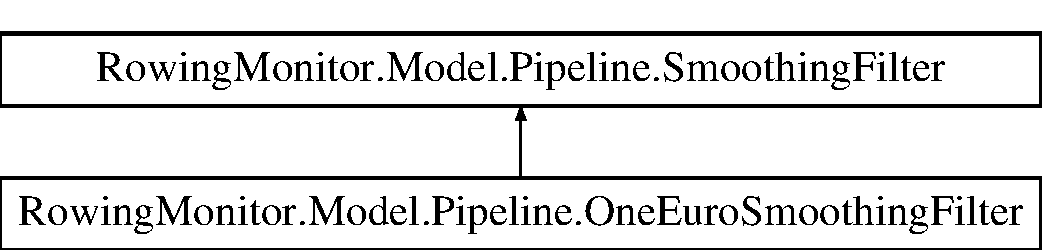
\includegraphics[height=2.000000cm]{class_rowing_monitor_1_1_model_1_1_pipeline_1_1_one_euro_smoothing_filter}
\end{center}
\end{figure}
\subsection*{Public Member Functions}
\begin{DoxyCompactItemize}
\item 
\hyperlink{class_rowing_monitor_1_1_model_1_1_pipeline_1_1_one_euro_smoothing_filter_a40e995e638198ea34d3c233663f6462c}{One\+Euro\+Smoothing\+Filter} (\hyperlink{namespace_rowing_monitor_1_1_model_1_1_util_a01e1a06061533b246feb7421c9d0107f}{Data\+Stream\+Type} output\+Data\+Stream\+Type)
\item 
override void \hyperlink{class_rowing_monitor_1_1_model_1_1_pipeline_1_1_one_euro_smoothing_filter_a2e518ce98440b3004aaf1af9a4eba399}{Update} (\hyperlink{struct_rowing_monitor_1_1_model_1_1_util_1_1_joint_data}{Joint\+Data} joint\+Data)
\item 
override \hyperlink{struct_rowing_monitor_1_1_model_1_1_util_1_1_joint_data}{Joint\+Data} \hyperlink{class_rowing_monitor_1_1_model_1_1_pipeline_1_1_one_euro_smoothing_filter_afd860237def583deb4499bc3c9fac868}{Smooth} (\hyperlink{struct_rowing_monitor_1_1_model_1_1_util_1_1_joint_data}{Joint\+Data} joint\+Data)
\end{DoxyCompactItemize}
\subsection*{Static Public Member Functions}
\begin{DoxyCompactItemize}
\item 
static Dictionary$<$ Joint\+Type, Dictionary$<$ String, Double $>$ $>$ \hyperlink{class_rowing_monitor_1_1_model_1_1_pipeline_1_1_one_euro_smoothing_filter_ab7a606c7bb286da8df457e553dc987eb}{Init\+Cutoff\+Dictionary} (Double value)
\begin{DoxyCompactList}\small\item\em Initliazies a dictionary of all joint types with a given value. \end{DoxyCompactList}\end{DoxyCompactItemize}
\subsection*{Protected Member Functions}
\begin{DoxyCompactItemize}
\item 
override void \hyperlink{class_rowing_monitor_1_1_model_1_1_pipeline_1_1_one_euro_smoothing_filter_ab4f64e95b9e02fb1562aeee79a75e695}{On\+Smoothed\+Frame\+Finished} (\hyperlink{class_rowing_monitor_1_1_model_1_1_smoothed_frame_arrived_event_args}{Smoothed\+Frame\+Arrived\+Event\+Args} e)
\end{DoxyCompactItemize}
\subsection*{Properties}
\begin{DoxyCompactItemize}
\item 
Double \hyperlink{class_rowing_monitor_1_1_model_1_1_pipeline_1_1_one_euro_smoothing_filter_aa9fe6be1fe6687a2fe7e1f8a77864527}{Beta}\hspace{0.3cm}{\ttfamily  \mbox{[}get, set\mbox{]}}
\item 
double \hyperlink{class_rowing_monitor_1_1_model_1_1_pipeline_1_1_one_euro_smoothing_filter_a8bb01ead704c4df8a684e64789762a7d}{Fcmin}\hspace{0.3cm}{\ttfamily  \mbox{[}get, set\mbox{]}}
\item 
Dictionary$<$ Joint\+Type, Dictionary$<$ string, double $>$ $>$ \hyperlink{class_rowing_monitor_1_1_model_1_1_pipeline_1_1_one_euro_smoothing_filter_a25584ff866652d0985ff677725a32f77}{Mincutoff}\hspace{0.3cm}{\ttfamily  \mbox{[}get, set\mbox{]}}
\end{DoxyCompactItemize}
\subsection*{Additional Inherited Members}


\subsection{Constructor \& Destructor Documentation}
\mbox{\Hypertarget{class_rowing_monitor_1_1_model_1_1_pipeline_1_1_one_euro_smoothing_filter_a40e995e638198ea34d3c233663f6462c}\label{class_rowing_monitor_1_1_model_1_1_pipeline_1_1_one_euro_smoothing_filter_a40e995e638198ea34d3c233663f6462c}} 
\index{Rowing\+Monitor\+::\+Model\+::\+Pipeline\+::\+One\+Euro\+Smoothing\+Filter@{Rowing\+Monitor\+::\+Model\+::\+Pipeline\+::\+One\+Euro\+Smoothing\+Filter}!One\+Euro\+Smoothing\+Filter@{One\+Euro\+Smoothing\+Filter}}
\index{One\+Euro\+Smoothing\+Filter@{One\+Euro\+Smoothing\+Filter}!Rowing\+Monitor\+::\+Model\+::\+Pipeline\+::\+One\+Euro\+Smoothing\+Filter@{Rowing\+Monitor\+::\+Model\+::\+Pipeline\+::\+One\+Euro\+Smoothing\+Filter}}
\subsubsection{\texorpdfstring{One\+Euro\+Smoothing\+Filter()}{OneEuroSmoothingFilter()}}
{\footnotesize\ttfamily Rowing\+Monitor.\+Model.\+Pipeline.\+One\+Euro\+Smoothing\+Filter.\+One\+Euro\+Smoothing\+Filter (\begin{DoxyParamCaption}\item[{\hyperlink{namespace_rowing_monitor_1_1_model_1_1_util_a01e1a06061533b246feb7421c9d0107f}{Data\+Stream\+Type}}]{output\+Data\+Stream\+Type }\end{DoxyParamCaption})}



\subsection{Member Function Documentation}
\mbox{\Hypertarget{class_rowing_monitor_1_1_model_1_1_pipeline_1_1_one_euro_smoothing_filter_ab7a606c7bb286da8df457e553dc987eb}\label{class_rowing_monitor_1_1_model_1_1_pipeline_1_1_one_euro_smoothing_filter_ab7a606c7bb286da8df457e553dc987eb}} 
\index{Rowing\+Monitor\+::\+Model\+::\+Pipeline\+::\+One\+Euro\+Smoothing\+Filter@{Rowing\+Monitor\+::\+Model\+::\+Pipeline\+::\+One\+Euro\+Smoothing\+Filter}!Init\+Cutoff\+Dictionary@{Init\+Cutoff\+Dictionary}}
\index{Init\+Cutoff\+Dictionary@{Init\+Cutoff\+Dictionary}!Rowing\+Monitor\+::\+Model\+::\+Pipeline\+::\+One\+Euro\+Smoothing\+Filter@{Rowing\+Monitor\+::\+Model\+::\+Pipeline\+::\+One\+Euro\+Smoothing\+Filter}}
\subsubsection{\texorpdfstring{Init\+Cutoff\+Dictionary()}{InitCutoffDictionary()}}
{\footnotesize\ttfamily static Dictionary$<$Joint\+Type, Dictionary$<$String, Double$>$ $>$ Rowing\+Monitor.\+Model.\+Pipeline.\+One\+Euro\+Smoothing\+Filter.\+Init\+Cutoff\+Dictionary (\begin{DoxyParamCaption}\item[{Double}]{value }\end{DoxyParamCaption})\hspace{0.3cm}{\ttfamily [static]}}



Initliazies a dictionary of all joint types with a given value. 


\begin{DoxyParams}{Parameters}
{\em value} & \\
\hline
\end{DoxyParams}
\begin{DoxyReturn}{Returns}

\end{DoxyReturn}
\mbox{\Hypertarget{class_rowing_monitor_1_1_model_1_1_pipeline_1_1_one_euro_smoothing_filter_ab4f64e95b9e02fb1562aeee79a75e695}\label{class_rowing_monitor_1_1_model_1_1_pipeline_1_1_one_euro_smoothing_filter_ab4f64e95b9e02fb1562aeee79a75e695}} 
\index{Rowing\+Monitor\+::\+Model\+::\+Pipeline\+::\+One\+Euro\+Smoothing\+Filter@{Rowing\+Monitor\+::\+Model\+::\+Pipeline\+::\+One\+Euro\+Smoothing\+Filter}!On\+Smoothed\+Frame\+Finished@{On\+Smoothed\+Frame\+Finished}}
\index{On\+Smoothed\+Frame\+Finished@{On\+Smoothed\+Frame\+Finished}!Rowing\+Monitor\+::\+Model\+::\+Pipeline\+::\+One\+Euro\+Smoothing\+Filter@{Rowing\+Monitor\+::\+Model\+::\+Pipeline\+::\+One\+Euro\+Smoothing\+Filter}}
\subsubsection{\texorpdfstring{On\+Smoothed\+Frame\+Finished()}{OnSmoothedFrameFinished()}}
{\footnotesize\ttfamily override void Rowing\+Monitor.\+Model.\+Pipeline.\+One\+Euro\+Smoothing\+Filter.\+On\+Smoothed\+Frame\+Finished (\begin{DoxyParamCaption}\item[{\hyperlink{class_rowing_monitor_1_1_model_1_1_smoothed_frame_arrived_event_args}{Smoothed\+Frame\+Arrived\+Event\+Args}}]{e }\end{DoxyParamCaption})\hspace{0.3cm}{\ttfamily [protected]}, {\ttfamily [virtual]}}



Reimplemented from \hyperlink{class_rowing_monitor_1_1_model_1_1_pipeline_1_1_smoothing_filter_ac47b399ad4ae1ad899f5e571d6f6c05c}{Rowing\+Monitor.\+Model.\+Pipeline.\+Smoothing\+Filter}.

\mbox{\Hypertarget{class_rowing_monitor_1_1_model_1_1_pipeline_1_1_one_euro_smoothing_filter_afd860237def583deb4499bc3c9fac868}\label{class_rowing_monitor_1_1_model_1_1_pipeline_1_1_one_euro_smoothing_filter_afd860237def583deb4499bc3c9fac868}} 
\index{Rowing\+Monitor\+::\+Model\+::\+Pipeline\+::\+One\+Euro\+Smoothing\+Filter@{Rowing\+Monitor\+::\+Model\+::\+Pipeline\+::\+One\+Euro\+Smoothing\+Filter}!Smooth@{Smooth}}
\index{Smooth@{Smooth}!Rowing\+Monitor\+::\+Model\+::\+Pipeline\+::\+One\+Euro\+Smoothing\+Filter@{Rowing\+Monitor\+::\+Model\+::\+Pipeline\+::\+One\+Euro\+Smoothing\+Filter}}
\subsubsection{\texorpdfstring{Smooth()}{Smooth()}}
{\footnotesize\ttfamily override \hyperlink{struct_rowing_monitor_1_1_model_1_1_util_1_1_joint_data}{Joint\+Data} Rowing\+Monitor.\+Model.\+Pipeline.\+One\+Euro\+Smoothing\+Filter.\+Smooth (\begin{DoxyParamCaption}\item[{\hyperlink{struct_rowing_monitor_1_1_model_1_1_util_1_1_joint_data}{Joint\+Data}}]{joint\+Data }\end{DoxyParamCaption})\hspace{0.3cm}{\ttfamily [virtual]}}



Implements \hyperlink{class_rowing_monitor_1_1_model_1_1_pipeline_1_1_smoothing_filter_a65ba6a5a48fbf5a51fb564dbeefc95fe}{Rowing\+Monitor.\+Model.\+Pipeline.\+Smoothing\+Filter}.

\mbox{\Hypertarget{class_rowing_monitor_1_1_model_1_1_pipeline_1_1_one_euro_smoothing_filter_a2e518ce98440b3004aaf1af9a4eba399}\label{class_rowing_monitor_1_1_model_1_1_pipeline_1_1_one_euro_smoothing_filter_a2e518ce98440b3004aaf1af9a4eba399}} 
\index{Rowing\+Monitor\+::\+Model\+::\+Pipeline\+::\+One\+Euro\+Smoothing\+Filter@{Rowing\+Monitor\+::\+Model\+::\+Pipeline\+::\+One\+Euro\+Smoothing\+Filter}!Update@{Update}}
\index{Update@{Update}!Rowing\+Monitor\+::\+Model\+::\+Pipeline\+::\+One\+Euro\+Smoothing\+Filter@{Rowing\+Monitor\+::\+Model\+::\+Pipeline\+::\+One\+Euro\+Smoothing\+Filter}}
\subsubsection{\texorpdfstring{Update()}{Update()}}
{\footnotesize\ttfamily override void Rowing\+Monitor.\+Model.\+Pipeline.\+One\+Euro\+Smoothing\+Filter.\+Update (\begin{DoxyParamCaption}\item[{\hyperlink{struct_rowing_monitor_1_1_model_1_1_util_1_1_joint_data}{Joint\+Data}}]{joint\+Data }\end{DoxyParamCaption})\hspace{0.3cm}{\ttfamily [virtual]}}



Implements \hyperlink{class_rowing_monitor_1_1_model_1_1_pipeline_1_1_smoothing_filter_a6f017782fee0747d4ece9ec3ffea6115}{Rowing\+Monitor.\+Model.\+Pipeline.\+Smoothing\+Filter}.



\subsection{Property Documentation}
\mbox{\Hypertarget{class_rowing_monitor_1_1_model_1_1_pipeline_1_1_one_euro_smoothing_filter_aa9fe6be1fe6687a2fe7e1f8a77864527}\label{class_rowing_monitor_1_1_model_1_1_pipeline_1_1_one_euro_smoothing_filter_aa9fe6be1fe6687a2fe7e1f8a77864527}} 
\index{Rowing\+Monitor\+::\+Model\+::\+Pipeline\+::\+One\+Euro\+Smoothing\+Filter@{Rowing\+Monitor\+::\+Model\+::\+Pipeline\+::\+One\+Euro\+Smoothing\+Filter}!Beta@{Beta}}
\index{Beta@{Beta}!Rowing\+Monitor\+::\+Model\+::\+Pipeline\+::\+One\+Euro\+Smoothing\+Filter@{Rowing\+Monitor\+::\+Model\+::\+Pipeline\+::\+One\+Euro\+Smoothing\+Filter}}
\subsubsection{\texorpdfstring{Beta}{Beta}}
{\footnotesize\ttfamily Double Rowing\+Monitor.\+Model.\+Pipeline.\+One\+Euro\+Smoothing\+Filter.\+Beta\hspace{0.3cm}{\ttfamily [get]}, {\ttfamily [set]}}

\mbox{\Hypertarget{class_rowing_monitor_1_1_model_1_1_pipeline_1_1_one_euro_smoothing_filter_a8bb01ead704c4df8a684e64789762a7d}\label{class_rowing_monitor_1_1_model_1_1_pipeline_1_1_one_euro_smoothing_filter_a8bb01ead704c4df8a684e64789762a7d}} 
\index{Rowing\+Monitor\+::\+Model\+::\+Pipeline\+::\+One\+Euro\+Smoothing\+Filter@{Rowing\+Monitor\+::\+Model\+::\+Pipeline\+::\+One\+Euro\+Smoothing\+Filter}!Fcmin@{Fcmin}}
\index{Fcmin@{Fcmin}!Rowing\+Monitor\+::\+Model\+::\+Pipeline\+::\+One\+Euro\+Smoothing\+Filter@{Rowing\+Monitor\+::\+Model\+::\+Pipeline\+::\+One\+Euro\+Smoothing\+Filter}}
\subsubsection{\texorpdfstring{Fcmin}{Fcmin}}
{\footnotesize\ttfamily double Rowing\+Monitor.\+Model.\+Pipeline.\+One\+Euro\+Smoothing\+Filter.\+Fcmin\hspace{0.3cm}{\ttfamily [get]}, {\ttfamily [set]}}

\mbox{\Hypertarget{class_rowing_monitor_1_1_model_1_1_pipeline_1_1_one_euro_smoothing_filter_a25584ff866652d0985ff677725a32f77}\label{class_rowing_monitor_1_1_model_1_1_pipeline_1_1_one_euro_smoothing_filter_a25584ff866652d0985ff677725a32f77}} 
\index{Rowing\+Monitor\+::\+Model\+::\+Pipeline\+::\+One\+Euro\+Smoothing\+Filter@{Rowing\+Monitor\+::\+Model\+::\+Pipeline\+::\+One\+Euro\+Smoothing\+Filter}!Mincutoff@{Mincutoff}}
\index{Mincutoff@{Mincutoff}!Rowing\+Monitor\+::\+Model\+::\+Pipeline\+::\+One\+Euro\+Smoothing\+Filter@{Rowing\+Monitor\+::\+Model\+::\+Pipeline\+::\+One\+Euro\+Smoothing\+Filter}}
\subsubsection{\texorpdfstring{Mincutoff}{Mincutoff}}
{\footnotesize\ttfamily Dictionary$<$Joint\+Type, Dictionary$<$string, double$>$ $>$ Rowing\+Monitor.\+Model.\+Pipeline.\+One\+Euro\+Smoothing\+Filter.\+Mincutoff\hspace{0.3cm}{\ttfamily [get]}, {\ttfamily [set]}}



The documentation for this class was generated from the following file\+:\begin{DoxyCompactItemize}
\item 
Model/\+Pipeline/\hyperlink{_one_euro_smoothing_filter_8cs}{One\+Euro\+Smoothing\+Filter.\+cs}\end{DoxyCompactItemize}

\hypertarget{class_rowing_monitor_1_1_view_1_1_page1}{}\section{Rowing\+Monitor.\+View.\+Page1 Class Reference}
\label{class_rowing_monitor_1_1_view_1_1_page1}\index{Rowing\+Monitor.\+View.\+Page1@{Rowing\+Monitor.\+View.\+Page1}}


\hyperlink{class_rowing_monitor_1_1_view_1_1_page1}{Page1}  


Inheritance diagram for Rowing\+Monitor.\+View.\+Page1\+:\begin{figure}[H]
\begin{center}
\leavevmode
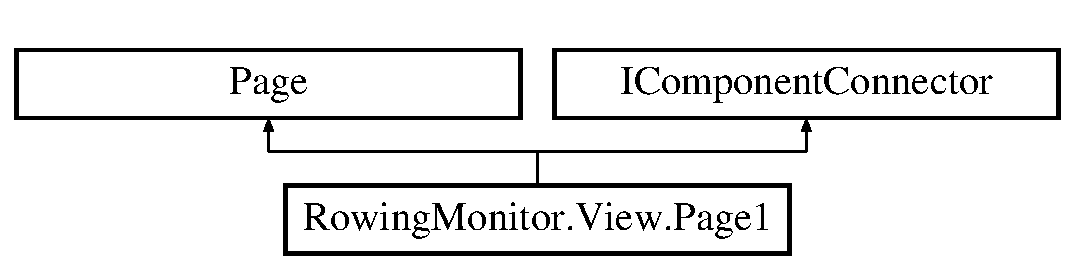
\includegraphics[height=2.000000cm]{class_rowing_monitor_1_1_view_1_1_page1}
\end{center}
\end{figure}
\subsection*{Public Member Functions}
\begin{DoxyCompactItemize}
\item 
void \hyperlink{class_rowing_monitor_1_1_view_1_1_page1_adf20b2105a2051a245d128555ee9b568}{Initialize\+Component} ()
\begin{DoxyCompactList}\small\item\em Initialize\+Component \end{DoxyCompactList}\end{DoxyCompactItemize}


\subsection{Detailed Description}
\hyperlink{class_rowing_monitor_1_1_view_1_1_page1}{Page1} 



\subsection{Member Function Documentation}
\mbox{\Hypertarget{class_rowing_monitor_1_1_view_1_1_page1_adf20b2105a2051a245d128555ee9b568}\label{class_rowing_monitor_1_1_view_1_1_page1_adf20b2105a2051a245d128555ee9b568}} 
\index{Rowing\+Monitor\+::\+View\+::\+Page1@{Rowing\+Monitor\+::\+View\+::\+Page1}!Initialize\+Component@{Initialize\+Component}}
\index{Initialize\+Component@{Initialize\+Component}!Rowing\+Monitor\+::\+View\+::\+Page1@{Rowing\+Monitor\+::\+View\+::\+Page1}}
\subsubsection{\texorpdfstring{Initialize\+Component()}{InitializeComponent()}}
{\footnotesize\ttfamily void Rowing\+Monitor.\+View.\+Page1.\+Initialize\+Component (\begin{DoxyParamCaption}{ }\end{DoxyParamCaption})}



Initialize\+Component 



The documentation for this class was generated from the following file\+:\begin{DoxyCompactItemize}
\item 
obj/\+Debug/\+View/\hyperlink{_page1_8g_8i_8cs}{Page1.\+g.\+i.\+cs}\end{DoxyCompactItemize}

\hypertarget{struct_rowing_monitor_1_1_model_1_1_util_1_1_plot_data}{}\section{Rowing\+Monitor.\+Model.\+Util.\+Plot\+Data Struct Reference}
\label{struct_rowing_monitor_1_1_model_1_1_util_1_1_plot_data}\index{Rowing\+Monitor.\+Model.\+Util.\+Plot\+Data@{Rowing\+Monitor.\+Model.\+Util.\+Plot\+Data}}
\subsection*{Properties}
\begin{DoxyCompactItemize}
\item 
double \hyperlink{struct_rowing_monitor_1_1_model_1_1_util_1_1_plot_data_aecf4f967ff34d6f3ff541792a3de2cb2}{X}\hspace{0.3cm}{\ttfamily  \mbox{[}get, set\mbox{]}}
\item 
double \hyperlink{struct_rowing_monitor_1_1_model_1_1_util_1_1_plot_data_ad481a32ecc84d09b772a1e7737728e46}{Y}\hspace{0.3cm}{\ttfamily  \mbox{[}get, set\mbox{]}}
\item 
string \hyperlink{struct_rowing_monitor_1_1_model_1_1_util_1_1_plot_data_a1ea10a21ea1ba58e32f59a6fe97d3f40}{Annotation}\hspace{0.3cm}{\ttfamily  \mbox{[}get, set\mbox{]}}
\item 
\hyperlink{namespace_rowing_monitor_1_1_model_1_1_util_a01e1a06061533b246feb7421c9d0107f}{Data\+Stream\+Type} \hyperlink{struct_rowing_monitor_1_1_model_1_1_util_1_1_plot_data_a774cc0b6b03996964e6bde85b993ca2d}{Data\+Stream\+Type}\hspace{0.3cm}{\ttfamily  \mbox{[}get, set\mbox{]}}
\end{DoxyCompactItemize}


\subsection{Property Documentation}
\mbox{\Hypertarget{struct_rowing_monitor_1_1_model_1_1_util_1_1_plot_data_a1ea10a21ea1ba58e32f59a6fe97d3f40}\label{struct_rowing_monitor_1_1_model_1_1_util_1_1_plot_data_a1ea10a21ea1ba58e32f59a6fe97d3f40}} 
\index{Rowing\+Monitor\+::\+Model\+::\+Util\+::\+Plot\+Data@{Rowing\+Monitor\+::\+Model\+::\+Util\+::\+Plot\+Data}!Annotation@{Annotation}}
\index{Annotation@{Annotation}!Rowing\+Monitor\+::\+Model\+::\+Util\+::\+Plot\+Data@{Rowing\+Monitor\+::\+Model\+::\+Util\+::\+Plot\+Data}}
\subsubsection{\texorpdfstring{Annotation}{Annotation}}
{\footnotesize\ttfamily string Rowing\+Monitor.\+Model.\+Util.\+Plot\+Data.\+Annotation\hspace{0.3cm}{\ttfamily [get]}, {\ttfamily [set]}}

\mbox{\Hypertarget{struct_rowing_monitor_1_1_model_1_1_util_1_1_plot_data_a774cc0b6b03996964e6bde85b993ca2d}\label{struct_rowing_monitor_1_1_model_1_1_util_1_1_plot_data_a774cc0b6b03996964e6bde85b993ca2d}} 
\index{Rowing\+Monitor\+::\+Model\+::\+Util\+::\+Plot\+Data@{Rowing\+Monitor\+::\+Model\+::\+Util\+::\+Plot\+Data}!Data\+Stream\+Type@{Data\+Stream\+Type}}
\index{Data\+Stream\+Type@{Data\+Stream\+Type}!Rowing\+Monitor\+::\+Model\+::\+Util\+::\+Plot\+Data@{Rowing\+Monitor\+::\+Model\+::\+Util\+::\+Plot\+Data}}
\subsubsection{\texorpdfstring{Data\+Stream\+Type}{DataStreamType}}
{\footnotesize\ttfamily \hyperlink{namespace_rowing_monitor_1_1_model_1_1_util_a01e1a06061533b246feb7421c9d0107f}{Data\+Stream\+Type} Rowing\+Monitor.\+Model.\+Util.\+Plot\+Data.\+Data\+Stream\+Type\hspace{0.3cm}{\ttfamily [get]}, {\ttfamily [set]}}

\mbox{\Hypertarget{struct_rowing_monitor_1_1_model_1_1_util_1_1_plot_data_aecf4f967ff34d6f3ff541792a3de2cb2}\label{struct_rowing_monitor_1_1_model_1_1_util_1_1_plot_data_aecf4f967ff34d6f3ff541792a3de2cb2}} 
\index{Rowing\+Monitor\+::\+Model\+::\+Util\+::\+Plot\+Data@{Rowing\+Monitor\+::\+Model\+::\+Util\+::\+Plot\+Data}!X@{X}}
\index{X@{X}!Rowing\+Monitor\+::\+Model\+::\+Util\+::\+Plot\+Data@{Rowing\+Monitor\+::\+Model\+::\+Util\+::\+Plot\+Data}}
\subsubsection{\texorpdfstring{X}{X}}
{\footnotesize\ttfamily double Rowing\+Monitor.\+Model.\+Util.\+Plot\+Data.\+X\hspace{0.3cm}{\ttfamily [get]}, {\ttfamily [set]}}

\mbox{\Hypertarget{struct_rowing_monitor_1_1_model_1_1_util_1_1_plot_data_ad481a32ecc84d09b772a1e7737728e46}\label{struct_rowing_monitor_1_1_model_1_1_util_1_1_plot_data_ad481a32ecc84d09b772a1e7737728e46}} 
\index{Rowing\+Monitor\+::\+Model\+::\+Util\+::\+Plot\+Data@{Rowing\+Monitor\+::\+Model\+::\+Util\+::\+Plot\+Data}!Y@{Y}}
\index{Y@{Y}!Rowing\+Monitor\+::\+Model\+::\+Util\+::\+Plot\+Data@{Rowing\+Monitor\+::\+Model\+::\+Util\+::\+Plot\+Data}}
\subsubsection{\texorpdfstring{Y}{Y}}
{\footnotesize\ttfamily double Rowing\+Monitor.\+Model.\+Util.\+Plot\+Data.\+Y\hspace{0.3cm}{\ttfamily [get]}, {\ttfamily [set]}}



The documentation for this struct was generated from the following file\+:\begin{DoxyCompactItemize}
\item 
Model/\+Util/\hyperlink{_plot_data_handler_8cs}{Plot\+Data\+Handler.\+cs}\end{DoxyCompactItemize}

\hypertarget{class_rowing_monitor_1_1_model_1_1_util_1_1_plot_data_handler}{}\section{Rowing\+Monitor.\+Model.\+Util.\+Plot\+Data\+Handler Class Reference}
\label{class_rowing_monitor_1_1_model_1_1_util_1_1_plot_data_handler}\index{Rowing\+Monitor.\+Model.\+Util.\+Plot\+Data\+Handler@{Rowing\+Monitor.\+Model.\+Util.\+Plot\+Data\+Handler}}


The documentation for this class was generated from the following file\+:\begin{DoxyCompactItemize}
\item 
Model/\+Util/\hyperlink{_plot_data_handler_8cs}{Plot\+Data\+Handler.\+cs}\end{DoxyCompactItemize}

\hypertarget{struct_rowing_monitor_1_1_model_1_1_util_1_1_curve_fitting_1_1_quadratic_function_parameters}{}\section{Rowing\+Monitor.\+Model.\+Util.\+Curve\+Fitting.\+Quadratic\+Function\+Parameters Struct Reference}
\label{struct_rowing_monitor_1_1_model_1_1_util_1_1_curve_fitting_1_1_quadratic_function_parameters}\index{Rowing\+Monitor.\+Model.\+Util.\+Curve\+Fitting.\+Quadratic\+Function\+Parameters@{Rowing\+Monitor.\+Model.\+Util.\+Curve\+Fitting.\+Quadratic\+Function\+Parameters}}
\subsection*{Public Attributes}
\begin{DoxyCompactItemize}
\item 
double \hyperlink{struct_rowing_monitor_1_1_model_1_1_util_1_1_curve_fitting_1_1_quadratic_function_parameters_a32e4362875df9f14ce040d57678e2788}{a}
\item 
double \hyperlink{struct_rowing_monitor_1_1_model_1_1_util_1_1_curve_fitting_1_1_quadratic_function_parameters_afe1a5177263ae1fa5a9077a0c5747b95}{b}
\item 
double \hyperlink{struct_rowing_monitor_1_1_model_1_1_util_1_1_curve_fitting_1_1_quadratic_function_parameters_a9e1baacfac496277b584a696bc83bbba}{c}
\item 
double \hyperlink{struct_rowing_monitor_1_1_model_1_1_util_1_1_curve_fitting_1_1_quadratic_function_parameters_ac0528b38840754899c904c31efd81545}{x\+Max}
\item 
double \hyperlink{struct_rowing_monitor_1_1_model_1_1_util_1_1_curve_fitting_1_1_quadratic_function_parameters_a7265f213951d92146c03ddc6235964f5}{y\+Max}
\end{DoxyCompactItemize}
\subsection*{Properties}
\begin{DoxyCompactItemize}
\item 
double \hyperlink{struct_rowing_monitor_1_1_model_1_1_util_1_1_curve_fitting_1_1_quadratic_function_parameters_ad636ac64e2f8404cae7d100a95d543ce}{A}\hspace{0.3cm}{\ttfamily  \mbox{[}get, set\mbox{]}}
\item 
double \hyperlink{struct_rowing_monitor_1_1_model_1_1_util_1_1_curve_fitting_1_1_quadratic_function_parameters_a74b2faac51507b9c925a2ee9185605e2}{B}\hspace{0.3cm}{\ttfamily  \mbox{[}get, set\mbox{]}}
\item 
double \hyperlink{struct_rowing_monitor_1_1_model_1_1_util_1_1_curve_fitting_1_1_quadratic_function_parameters_a2c26f634699927ecf6586043bf7a134b}{C}\hspace{0.3cm}{\ttfamily  \mbox{[}get, set\mbox{]}}
\item 
double \hyperlink{struct_rowing_monitor_1_1_model_1_1_util_1_1_curve_fitting_1_1_quadratic_function_parameters_a40123a6904fd646645844bd2e23bbaef}{X\+Max}\hspace{0.3cm}{\ttfamily  \mbox{[}get, set\mbox{]}}
\item 
double \hyperlink{struct_rowing_monitor_1_1_model_1_1_util_1_1_curve_fitting_1_1_quadratic_function_parameters_a873310b852028fc7ec7629bb3fb49f86}{Y\+Max}\hspace{0.3cm}{\ttfamily  \mbox{[}get, set\mbox{]}}
\end{DoxyCompactItemize}


\subsection{Member Data Documentation}
\mbox{\Hypertarget{struct_rowing_monitor_1_1_model_1_1_util_1_1_curve_fitting_1_1_quadratic_function_parameters_a32e4362875df9f14ce040d57678e2788}\label{struct_rowing_monitor_1_1_model_1_1_util_1_1_curve_fitting_1_1_quadratic_function_parameters_a32e4362875df9f14ce040d57678e2788}} 
\index{Rowing\+Monitor\+::\+Model\+::\+Util\+::\+Curve\+Fitting\+::\+Quadratic\+Function\+Parameters@{Rowing\+Monitor\+::\+Model\+::\+Util\+::\+Curve\+Fitting\+::\+Quadratic\+Function\+Parameters}!a@{a}}
\index{a@{a}!Rowing\+Monitor\+::\+Model\+::\+Util\+::\+Curve\+Fitting\+::\+Quadratic\+Function\+Parameters@{Rowing\+Monitor\+::\+Model\+::\+Util\+::\+Curve\+Fitting\+::\+Quadratic\+Function\+Parameters}}
\subsubsection{\texorpdfstring{a}{a}}
{\footnotesize\ttfamily double Rowing\+Monitor.\+Model.\+Util.\+Curve\+Fitting.\+Quadratic\+Function\+Parameters.\+a}

\mbox{\Hypertarget{struct_rowing_monitor_1_1_model_1_1_util_1_1_curve_fitting_1_1_quadratic_function_parameters_afe1a5177263ae1fa5a9077a0c5747b95}\label{struct_rowing_monitor_1_1_model_1_1_util_1_1_curve_fitting_1_1_quadratic_function_parameters_afe1a5177263ae1fa5a9077a0c5747b95}} 
\index{Rowing\+Monitor\+::\+Model\+::\+Util\+::\+Curve\+Fitting\+::\+Quadratic\+Function\+Parameters@{Rowing\+Monitor\+::\+Model\+::\+Util\+::\+Curve\+Fitting\+::\+Quadratic\+Function\+Parameters}!b@{b}}
\index{b@{b}!Rowing\+Monitor\+::\+Model\+::\+Util\+::\+Curve\+Fitting\+::\+Quadratic\+Function\+Parameters@{Rowing\+Monitor\+::\+Model\+::\+Util\+::\+Curve\+Fitting\+::\+Quadratic\+Function\+Parameters}}
\subsubsection{\texorpdfstring{b}{b}}
{\footnotesize\ttfamily double Rowing\+Monitor.\+Model.\+Util.\+Curve\+Fitting.\+Quadratic\+Function\+Parameters.\+b}

\mbox{\Hypertarget{struct_rowing_monitor_1_1_model_1_1_util_1_1_curve_fitting_1_1_quadratic_function_parameters_a9e1baacfac496277b584a696bc83bbba}\label{struct_rowing_monitor_1_1_model_1_1_util_1_1_curve_fitting_1_1_quadratic_function_parameters_a9e1baacfac496277b584a696bc83bbba}} 
\index{Rowing\+Monitor\+::\+Model\+::\+Util\+::\+Curve\+Fitting\+::\+Quadratic\+Function\+Parameters@{Rowing\+Monitor\+::\+Model\+::\+Util\+::\+Curve\+Fitting\+::\+Quadratic\+Function\+Parameters}!c@{c}}
\index{c@{c}!Rowing\+Monitor\+::\+Model\+::\+Util\+::\+Curve\+Fitting\+::\+Quadratic\+Function\+Parameters@{Rowing\+Monitor\+::\+Model\+::\+Util\+::\+Curve\+Fitting\+::\+Quadratic\+Function\+Parameters}}
\subsubsection{\texorpdfstring{c}{c}}
{\footnotesize\ttfamily double Rowing\+Monitor.\+Model.\+Util.\+Curve\+Fitting.\+Quadratic\+Function\+Parameters.\+c}

\mbox{\Hypertarget{struct_rowing_monitor_1_1_model_1_1_util_1_1_curve_fitting_1_1_quadratic_function_parameters_ac0528b38840754899c904c31efd81545}\label{struct_rowing_monitor_1_1_model_1_1_util_1_1_curve_fitting_1_1_quadratic_function_parameters_ac0528b38840754899c904c31efd81545}} 
\index{Rowing\+Monitor\+::\+Model\+::\+Util\+::\+Curve\+Fitting\+::\+Quadratic\+Function\+Parameters@{Rowing\+Monitor\+::\+Model\+::\+Util\+::\+Curve\+Fitting\+::\+Quadratic\+Function\+Parameters}!x\+Max@{x\+Max}}
\index{x\+Max@{x\+Max}!Rowing\+Monitor\+::\+Model\+::\+Util\+::\+Curve\+Fitting\+::\+Quadratic\+Function\+Parameters@{Rowing\+Monitor\+::\+Model\+::\+Util\+::\+Curve\+Fitting\+::\+Quadratic\+Function\+Parameters}}
\subsubsection{\texorpdfstring{x\+Max}{xMax}}
{\footnotesize\ttfamily double Rowing\+Monitor.\+Model.\+Util.\+Curve\+Fitting.\+Quadratic\+Function\+Parameters.\+x\+Max}

\mbox{\Hypertarget{struct_rowing_monitor_1_1_model_1_1_util_1_1_curve_fitting_1_1_quadratic_function_parameters_a7265f213951d92146c03ddc6235964f5}\label{struct_rowing_monitor_1_1_model_1_1_util_1_1_curve_fitting_1_1_quadratic_function_parameters_a7265f213951d92146c03ddc6235964f5}} 
\index{Rowing\+Monitor\+::\+Model\+::\+Util\+::\+Curve\+Fitting\+::\+Quadratic\+Function\+Parameters@{Rowing\+Monitor\+::\+Model\+::\+Util\+::\+Curve\+Fitting\+::\+Quadratic\+Function\+Parameters}!y\+Max@{y\+Max}}
\index{y\+Max@{y\+Max}!Rowing\+Monitor\+::\+Model\+::\+Util\+::\+Curve\+Fitting\+::\+Quadratic\+Function\+Parameters@{Rowing\+Monitor\+::\+Model\+::\+Util\+::\+Curve\+Fitting\+::\+Quadratic\+Function\+Parameters}}
\subsubsection{\texorpdfstring{y\+Max}{yMax}}
{\footnotesize\ttfamily double Rowing\+Monitor.\+Model.\+Util.\+Curve\+Fitting.\+Quadratic\+Function\+Parameters.\+y\+Max}



\subsection{Property Documentation}
\mbox{\Hypertarget{struct_rowing_monitor_1_1_model_1_1_util_1_1_curve_fitting_1_1_quadratic_function_parameters_ad636ac64e2f8404cae7d100a95d543ce}\label{struct_rowing_monitor_1_1_model_1_1_util_1_1_curve_fitting_1_1_quadratic_function_parameters_ad636ac64e2f8404cae7d100a95d543ce}} 
\index{Rowing\+Monitor\+::\+Model\+::\+Util\+::\+Curve\+Fitting\+::\+Quadratic\+Function\+Parameters@{Rowing\+Monitor\+::\+Model\+::\+Util\+::\+Curve\+Fitting\+::\+Quadratic\+Function\+Parameters}!A@{A}}
\index{A@{A}!Rowing\+Monitor\+::\+Model\+::\+Util\+::\+Curve\+Fitting\+::\+Quadratic\+Function\+Parameters@{Rowing\+Monitor\+::\+Model\+::\+Util\+::\+Curve\+Fitting\+::\+Quadratic\+Function\+Parameters}}
\subsubsection{\texorpdfstring{A}{A}}
{\footnotesize\ttfamily double Rowing\+Monitor.\+Model.\+Util.\+Curve\+Fitting.\+Quadratic\+Function\+Parameters.\+A\hspace{0.3cm}{\ttfamily [get]}, {\ttfamily [set]}}

\mbox{\Hypertarget{struct_rowing_monitor_1_1_model_1_1_util_1_1_curve_fitting_1_1_quadratic_function_parameters_a74b2faac51507b9c925a2ee9185605e2}\label{struct_rowing_monitor_1_1_model_1_1_util_1_1_curve_fitting_1_1_quadratic_function_parameters_a74b2faac51507b9c925a2ee9185605e2}} 
\index{Rowing\+Monitor\+::\+Model\+::\+Util\+::\+Curve\+Fitting\+::\+Quadratic\+Function\+Parameters@{Rowing\+Monitor\+::\+Model\+::\+Util\+::\+Curve\+Fitting\+::\+Quadratic\+Function\+Parameters}!B@{B}}
\index{B@{B}!Rowing\+Monitor\+::\+Model\+::\+Util\+::\+Curve\+Fitting\+::\+Quadratic\+Function\+Parameters@{Rowing\+Monitor\+::\+Model\+::\+Util\+::\+Curve\+Fitting\+::\+Quadratic\+Function\+Parameters}}
\subsubsection{\texorpdfstring{B}{B}}
{\footnotesize\ttfamily double Rowing\+Monitor.\+Model.\+Util.\+Curve\+Fitting.\+Quadratic\+Function\+Parameters.\+B\hspace{0.3cm}{\ttfamily [get]}, {\ttfamily [set]}}

\mbox{\Hypertarget{struct_rowing_monitor_1_1_model_1_1_util_1_1_curve_fitting_1_1_quadratic_function_parameters_a2c26f634699927ecf6586043bf7a134b}\label{struct_rowing_monitor_1_1_model_1_1_util_1_1_curve_fitting_1_1_quadratic_function_parameters_a2c26f634699927ecf6586043bf7a134b}} 
\index{Rowing\+Monitor\+::\+Model\+::\+Util\+::\+Curve\+Fitting\+::\+Quadratic\+Function\+Parameters@{Rowing\+Monitor\+::\+Model\+::\+Util\+::\+Curve\+Fitting\+::\+Quadratic\+Function\+Parameters}!C@{C}}
\index{C@{C}!Rowing\+Monitor\+::\+Model\+::\+Util\+::\+Curve\+Fitting\+::\+Quadratic\+Function\+Parameters@{Rowing\+Monitor\+::\+Model\+::\+Util\+::\+Curve\+Fitting\+::\+Quadratic\+Function\+Parameters}}
\subsubsection{\texorpdfstring{C}{C}}
{\footnotesize\ttfamily double Rowing\+Monitor.\+Model.\+Util.\+Curve\+Fitting.\+Quadratic\+Function\+Parameters.\+C\hspace{0.3cm}{\ttfamily [get]}, {\ttfamily [set]}}

\mbox{\Hypertarget{struct_rowing_monitor_1_1_model_1_1_util_1_1_curve_fitting_1_1_quadratic_function_parameters_a40123a6904fd646645844bd2e23bbaef}\label{struct_rowing_monitor_1_1_model_1_1_util_1_1_curve_fitting_1_1_quadratic_function_parameters_a40123a6904fd646645844bd2e23bbaef}} 
\index{Rowing\+Monitor\+::\+Model\+::\+Util\+::\+Curve\+Fitting\+::\+Quadratic\+Function\+Parameters@{Rowing\+Monitor\+::\+Model\+::\+Util\+::\+Curve\+Fitting\+::\+Quadratic\+Function\+Parameters}!X\+Max@{X\+Max}}
\index{X\+Max@{X\+Max}!Rowing\+Monitor\+::\+Model\+::\+Util\+::\+Curve\+Fitting\+::\+Quadratic\+Function\+Parameters@{Rowing\+Monitor\+::\+Model\+::\+Util\+::\+Curve\+Fitting\+::\+Quadratic\+Function\+Parameters}}
\subsubsection{\texorpdfstring{X\+Max}{XMax}}
{\footnotesize\ttfamily double Rowing\+Monitor.\+Model.\+Util.\+Curve\+Fitting.\+Quadratic\+Function\+Parameters.\+X\+Max\hspace{0.3cm}{\ttfamily [get]}, {\ttfamily [set]}}

\mbox{\Hypertarget{struct_rowing_monitor_1_1_model_1_1_util_1_1_curve_fitting_1_1_quadratic_function_parameters_a873310b852028fc7ec7629bb3fb49f86}\label{struct_rowing_monitor_1_1_model_1_1_util_1_1_curve_fitting_1_1_quadratic_function_parameters_a873310b852028fc7ec7629bb3fb49f86}} 
\index{Rowing\+Monitor\+::\+Model\+::\+Util\+::\+Curve\+Fitting\+::\+Quadratic\+Function\+Parameters@{Rowing\+Monitor\+::\+Model\+::\+Util\+::\+Curve\+Fitting\+::\+Quadratic\+Function\+Parameters}!Y\+Max@{Y\+Max}}
\index{Y\+Max@{Y\+Max}!Rowing\+Monitor\+::\+Model\+::\+Util\+::\+Curve\+Fitting\+::\+Quadratic\+Function\+Parameters@{Rowing\+Monitor\+::\+Model\+::\+Util\+::\+Curve\+Fitting\+::\+Quadratic\+Function\+Parameters}}
\subsubsection{\texorpdfstring{Y\+Max}{YMax}}
{\footnotesize\ttfamily double Rowing\+Monitor.\+Model.\+Util.\+Curve\+Fitting.\+Quadratic\+Function\+Parameters.\+Y\+Max\hspace{0.3cm}{\ttfamily [get]}, {\ttfamily [set]}}



The documentation for this struct was generated from the following file\+:\begin{DoxyCompactItemize}
\item 
Model/\+Util/\hyperlink{_curve_fitting_8cs}{Curve\+Fitting.\+cs}\end{DoxyCompactItemize}

\hypertarget{class_rowing_monitor_1_1_relay_command}{}\section{Rowing\+Monitor.\+Relay\+Command Class Reference}
\label{class_rowing_monitor_1_1_relay_command}\index{Rowing\+Monitor.\+Relay\+Command@{Rowing\+Monitor.\+Relay\+Command}}
Inheritance diagram for Rowing\+Monitor.\+Relay\+Command\+:\begin{figure}[H]
\begin{center}
\leavevmode
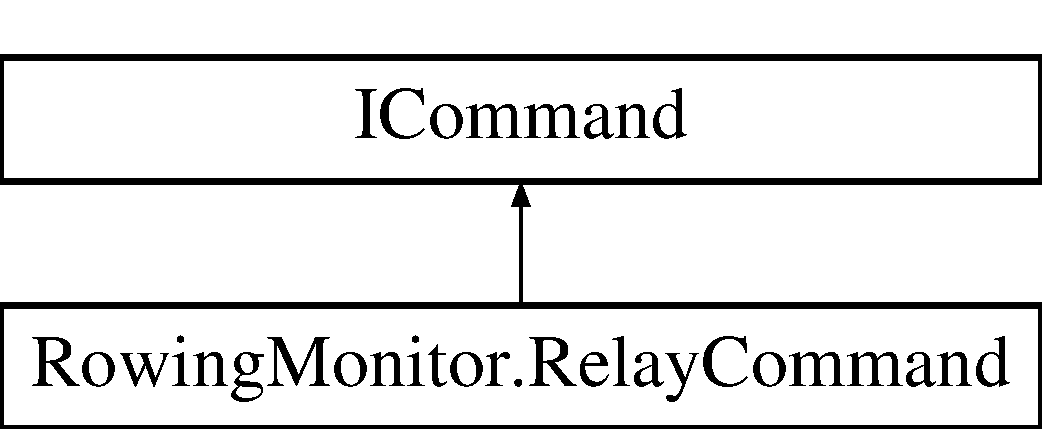
\includegraphics[height=2.000000cm]{class_rowing_monitor_1_1_relay_command}
\end{center}
\end{figure}
\subsection*{Public Member Functions}
\begin{DoxyCompactItemize}
\item 
\hyperlink{class_rowing_monitor_1_1_relay_command_a489257b2b64ff595ac8cf6f4dea07822}{Relay\+Command} (Action$<$ object $>$ execute)
\item 
\hyperlink{class_rowing_monitor_1_1_relay_command_a683db6291fb9d78a125cff700be862d6}{Relay\+Command} (Action$<$ object $>$ execute, Predicate$<$ object $>$ can\+Execute)
\item 
void \hyperlink{class_rowing_monitor_1_1_relay_command_ac4ca734c8e04bfb87cf1a1c295fb2d5b}{Execute} (object parameter)
\item 
bool \hyperlink{class_rowing_monitor_1_1_relay_command_a85fe9d9b44a1db38da8e1330d6715b30}{Can\+Execute} (object parameter)
\end{DoxyCompactItemize}
\subsection*{Properties}
\begin{DoxyCompactItemize}
\item 
Event\+Handler \hyperlink{class_rowing_monitor_1_1_relay_command_ae4dd035ea91a110089885a49c15fa525}{Can\+Execute\+Changed}
\end{DoxyCompactItemize}


\subsection{Constructor \& Destructor Documentation}
\mbox{\Hypertarget{class_rowing_monitor_1_1_relay_command_a489257b2b64ff595ac8cf6f4dea07822}\label{class_rowing_monitor_1_1_relay_command_a489257b2b64ff595ac8cf6f4dea07822}} 
\index{Rowing\+Monitor\+::\+Relay\+Command@{Rowing\+Monitor\+::\+Relay\+Command}!Relay\+Command@{Relay\+Command}}
\index{Relay\+Command@{Relay\+Command}!Rowing\+Monitor\+::\+Relay\+Command@{Rowing\+Monitor\+::\+Relay\+Command}}
\subsubsection{\texorpdfstring{Relay\+Command()}{RelayCommand()}\hspace{0.1cm}{\footnotesize\ttfamily [1/2]}}
{\footnotesize\ttfamily Rowing\+Monitor.\+Relay\+Command.\+Relay\+Command (\begin{DoxyParamCaption}\item[{Action$<$ object $>$}]{execute }\end{DoxyParamCaption})}

\mbox{\Hypertarget{class_rowing_monitor_1_1_relay_command_a683db6291fb9d78a125cff700be862d6}\label{class_rowing_monitor_1_1_relay_command_a683db6291fb9d78a125cff700be862d6}} 
\index{Rowing\+Monitor\+::\+Relay\+Command@{Rowing\+Monitor\+::\+Relay\+Command}!Relay\+Command@{Relay\+Command}}
\index{Relay\+Command@{Relay\+Command}!Rowing\+Monitor\+::\+Relay\+Command@{Rowing\+Monitor\+::\+Relay\+Command}}
\subsubsection{\texorpdfstring{Relay\+Command()}{RelayCommand()}\hspace{0.1cm}{\footnotesize\ttfamily [2/2]}}
{\footnotesize\ttfamily Rowing\+Monitor.\+Relay\+Command.\+Relay\+Command (\begin{DoxyParamCaption}\item[{Action$<$ object $>$}]{execute,  }\item[{Predicate$<$ object $>$}]{can\+Execute }\end{DoxyParamCaption})}



\subsection{Member Function Documentation}
\mbox{\Hypertarget{class_rowing_monitor_1_1_relay_command_a85fe9d9b44a1db38da8e1330d6715b30}\label{class_rowing_monitor_1_1_relay_command_a85fe9d9b44a1db38da8e1330d6715b30}} 
\index{Rowing\+Monitor\+::\+Relay\+Command@{Rowing\+Monitor\+::\+Relay\+Command}!Can\+Execute@{Can\+Execute}}
\index{Can\+Execute@{Can\+Execute}!Rowing\+Monitor\+::\+Relay\+Command@{Rowing\+Monitor\+::\+Relay\+Command}}
\subsubsection{\texorpdfstring{Can\+Execute()}{CanExecute()}}
{\footnotesize\ttfamily bool Rowing\+Monitor.\+Relay\+Command.\+Can\+Execute (\begin{DoxyParamCaption}\item[{object}]{parameter }\end{DoxyParamCaption})}

\mbox{\Hypertarget{class_rowing_monitor_1_1_relay_command_ac4ca734c8e04bfb87cf1a1c295fb2d5b}\label{class_rowing_monitor_1_1_relay_command_ac4ca734c8e04bfb87cf1a1c295fb2d5b}} 
\index{Rowing\+Monitor\+::\+Relay\+Command@{Rowing\+Monitor\+::\+Relay\+Command}!Execute@{Execute}}
\index{Execute@{Execute}!Rowing\+Monitor\+::\+Relay\+Command@{Rowing\+Monitor\+::\+Relay\+Command}}
\subsubsection{\texorpdfstring{Execute()}{Execute()}}
{\footnotesize\ttfamily void Rowing\+Monitor.\+Relay\+Command.\+Execute (\begin{DoxyParamCaption}\item[{object}]{parameter }\end{DoxyParamCaption})}



\subsection{Property Documentation}
\mbox{\Hypertarget{class_rowing_monitor_1_1_relay_command_ae4dd035ea91a110089885a49c15fa525}\label{class_rowing_monitor_1_1_relay_command_ae4dd035ea91a110089885a49c15fa525}} 
\index{Rowing\+Monitor\+::\+Relay\+Command@{Rowing\+Monitor\+::\+Relay\+Command}!Can\+Execute\+Changed@{Can\+Execute\+Changed}}
\index{Can\+Execute\+Changed@{Can\+Execute\+Changed}!Rowing\+Monitor\+::\+Relay\+Command@{Rowing\+Monitor\+::\+Relay\+Command}}
\subsubsection{\texorpdfstring{Can\+Execute\+Changed}{CanExecuteChanged}}
{\footnotesize\ttfamily Event\+Handler Rowing\+Monitor.\+Relay\+Command.\+Can\+Execute\+Changed\hspace{0.3cm}{\ttfamily [add]}, {\ttfamily [remove]}}



The documentation for this class was generated from the following file\+:\begin{DoxyCompactItemize}
\item 
Model/\+Util/\hyperlink{_relay_command_8cs}{Relay\+Command.\+cs}\end{DoxyCompactItemize}

\hypertarget{class_rowing_monitor_1_1_properties_1_1_resources}{}\section{Rowing\+Monitor.\+Properties.\+Resources Class Reference}
\label{class_rowing_monitor_1_1_properties_1_1_resources}\index{Rowing\+Monitor.\+Properties.\+Resources@{Rowing\+Monitor.\+Properties.\+Resources}}


Eine stark typisierte Ressourcenklasse zum Suchen von lokalisierten Zeichenfolgen usw.  


\subsection*{Properties}
\begin{DoxyCompactItemize}
\item 
static global\+::\+System.\+Resources.\+Resource\+Manager \hyperlink{class_rowing_monitor_1_1_properties_1_1_resources_ad922a285236bdd870f295d1094dc602d}{Resource\+Manager}\hspace{0.3cm}{\ttfamily  \mbox{[}get\mbox{]}}
\begin{DoxyCompactList}\small\item\em Gibt die zwischengespeicherte Resource\+Manager-\/\+Instanz zurück, die von dieser Klasse verwendet wird. \end{DoxyCompactList}\item 
static global\+::\+System.\+Globalization.\+Culture\+Info \hyperlink{class_rowing_monitor_1_1_properties_1_1_resources_a99dee899703451cc2050cff9b778058a}{Culture}\hspace{0.3cm}{\ttfamily  \mbox{[}get, set\mbox{]}}
\begin{DoxyCompactList}\small\item\em Überschreibt die Current\+U\+I\+Culture-\/\+Eigenschaft des aktuellen Threads für alle Ressourcenzuordnungen, die diese stark typisierte Ressourcenklasse verwenden. \end{DoxyCompactList}\item 
static string \hyperlink{class_rowing_monitor_1_1_properties_1_1_resources_a387e94c12ed72def984e5c51c268cf0a}{Catch\+Factor}\hspace{0.3cm}{\ttfamily  \mbox{[}get\mbox{]}}
\begin{DoxyCompactList}\small\item\em Sucht eine lokalisierte Zeichenfolge, die Catch factor (ms) ähnelt. \end{DoxyCompactList}\item 
static string \hyperlink{class_rowing_monitor_1_1_properties_1_1_resources_a1a12bdf0feea59667d2d272370806cfa}{Catch\+Trunk\+Angle\+Title}\hspace{0.3cm}{\ttfamily  \mbox{[}get\mbox{]}}
\begin{DoxyCompactList}\small\item\em Sucht eine lokalisierte Zeichenfolge, die Catch trunk angle ähnelt. \end{DoxyCompactList}\item 
static string \hyperlink{class_rowing_monitor_1_1_properties_1_1_resources_aaff4b4081f166baef8672bd7a8fb0a46}{Coach\+Message}\hspace{0.3cm}{\ttfamily  \mbox{[}get\mbox{]}}
\begin{DoxyCompactList}\small\item\em Sucht eine lokalisierte Zeichenfolge, die Start tracking with the dashboard layout for coaches. ähnelt. \end{DoxyCompactList}\item 
static string \hyperlink{class_rowing_monitor_1_1_properties_1_1_resources_a23437e7fcfbd5a143a7dcb88fd19ae11}{Coach\+Title}\hspace{0.3cm}{\ttfamily  \mbox{[}get\mbox{]}}
\begin{DoxyCompactList}\small\item\em Sucht eine lokalisierte Zeichenfolge, die Coach view ähnelt. \end{DoxyCompactList}\item 
static string \hyperlink{class_rowing_monitor_1_1_properties_1_1_resources_a31be075f6145a715b6449bd05c48a441}{Debug\+Message}\hspace{0.3cm}{\ttfamily  \mbox{[}get\mbox{]}}
\begin{DoxyCompactList}\small\item\em Sucht eine lokalisierte Zeichenfolge, die Start tracking and show all available evaluation elements. ähnelt. \end{DoxyCompactList}\item 
static string \hyperlink{class_rowing_monitor_1_1_properties_1_1_resources_ac197e44538c0c710513c11a63d98f236}{Debug\+Title}\hspace{0.3cm}{\ttfamily  \mbox{[}get\mbox{]}}
\begin{DoxyCompactList}\small\item\em Sucht eine lokalisierte Zeichenfolge, die Debug view ähnelt. \end{DoxyCompactList}\item 
static string \hyperlink{class_rowing_monitor_1_1_properties_1_1_resources_a82fbb12913d48de07a02c10dd756b575}{Failed\+Screenshot\+Status\+Text\+Format}\hspace{0.3cm}{\ttfamily  \mbox{[}get\mbox{]}}
\begin{DoxyCompactList}\small\item\em Sucht eine lokalisierte Zeichenfolge, die Failed to write screenshot to \{0\} ähnelt. \end{DoxyCompactList}\item 
static string \hyperlink{class_rowing_monitor_1_1_properties_1_1_resources_acd7d5d6ec683cf057f592a4376863aaf}{Finish\+Trunk\+Angle\+Title}\hspace{0.3cm}{\ttfamily  \mbox{[}get\mbox{]}}
\begin{DoxyCompactList}\small\item\em Sucht eine lokalisierte Zeichenfolge, die Finish trunk angle ähnelt. \end{DoxyCompactList}\item 
static string \hyperlink{class_rowing_monitor_1_1_properties_1_1_resources_a63d3b05296e1f16c61a2b7a9d1b3b651}{Frame\+Index}\hspace{0.3cm}{\ttfamily  \mbox{[}get\mbox{]}}
\begin{DoxyCompactList}\small\item\em Sucht eine lokalisierte Zeichenfolge, die Frame index ähnelt. \end{DoxyCompactList}\item 
static string \hyperlink{class_rowing_monitor_1_1_properties_1_1_resources_af4884ca8ac262911b1fc76c39483a14a}{Home\+Title}\hspace{0.3cm}{\ttfamily  \mbox{[}get\mbox{]}}
\begin{DoxyCompactList}\small\item\em Sucht eine lokalisierte Zeichenfolge, die Choose a view ähnelt. \end{DoxyCompactList}\item 
static string \hyperlink{class_rowing_monitor_1_1_properties_1_1_resources_a60670c6f75fd3d65281c6341933120b4}{Kinect\+Calibration\+Message}\hspace{0.3cm}{\ttfamily  \mbox{[}get\mbox{]}}
\begin{DoxyCompactList}\small\item\em Sucht eine lokalisierte Zeichenfolge, die Find a position for the Kinect sensor and trainee. The skeleton should stay green for the complete stroke to get the best results. ähnelt. \end{DoxyCompactList}\item 
static string \hyperlink{class_rowing_monitor_1_1_properties_1_1_resources_a609ea52354bf88d51d0cebd9bd48de8d}{Kinect\+Calibration\+Title}\hspace{0.3cm}{\ttfamily  \mbox{[}get\mbox{]}}
\begin{DoxyCompactList}\small\item\em Sucht eine lokalisierte Zeichenfolge, die Kinect calibration ähnelt. \end{DoxyCompactList}\item 
static string \hyperlink{class_rowing_monitor_1_1_properties_1_1_resources_a33975b96d05a09f0d029609632c10ff9}{Kinect\+Not\+Found\+Message}\hspace{0.3cm}{\ttfamily  \mbox{[}get\mbox{]}}
\begin{DoxyCompactList}\small\item\em Sucht eine lokalisierte Zeichenfolge, die Kinect not connected. ähnelt. \end{DoxyCompactList}\item 
static string \hyperlink{class_rowing_monitor_1_1_properties_1_1_resources_a24ae603ed8d743173db5ad95422f1b43}{Max\+Arms\+Velocity}\hspace{0.3cm}{\ttfamily  \mbox{[}get\mbox{]}}
\begin{DoxyCompactList}\small\item\em Sucht eine lokalisierte Zeichenfolge, die Maximum arms velocity (m/s) ähnelt. \end{DoxyCompactList}\item 
static string \hyperlink{class_rowing_monitor_1_1_properties_1_1_resources_a719188712de0b0ca68430d55ef6e056a}{Max\+Catch\+Trunk\+Angle}\hspace{0.3cm}{\ttfamily  \mbox{[}get\mbox{]}}
\begin{DoxyCompactList}\small\item\em Sucht eine lokalisierte Zeichenfolge, die Maximum catch trunk angle (°) ähnelt. \end{DoxyCompactList}\item 
static string \hyperlink{class_rowing_monitor_1_1_properties_1_1_resources_ab2e04d859eccef5e7fe84566c5d19a9e}{Max\+Finish\+Trunk\+Angle}\hspace{0.3cm}{\ttfamily  \mbox{[}get\mbox{]}}
\begin{DoxyCompactList}\small\item\em Sucht eine lokalisierte Zeichenfolge, die Maximum finish trunk angle (°) ähnelt. \end{DoxyCompactList}\item 
static string \hyperlink{class_rowing_monitor_1_1_properties_1_1_resources_ae64ee05cc7efe5061d819604243cc329}{Max\+Handle\+Velocity}\hspace{0.3cm}{\ttfamily  \mbox{[}get\mbox{]}}
\begin{DoxyCompactList}\small\item\em Sucht eine lokalisierte Zeichenfolge, die Maximum handle velocity (m/s) ähnelt. \end{DoxyCompactList}\item 
static string \hyperlink{class_rowing_monitor_1_1_properties_1_1_resources_a1be32a40d9aabe3ccd2a5e2a4c13c5e6}{Max\+Legs\+Velocity}\hspace{0.3cm}{\ttfamily  \mbox{[}get\mbox{]}}
\begin{DoxyCompactList}\small\item\em Sucht eine lokalisierte Zeichenfolge, die Maximum legs velocity (m/s) ähnelt. \end{DoxyCompactList}\item 
static string \hyperlink{class_rowing_monitor_1_1_properties_1_1_resources_a55adc5e7b70ad437f1d5cc217fd3e799}{Max\+Trunk\+Velocity}\hspace{0.3cm}{\ttfamily  \mbox{[}get\mbox{]}}
\begin{DoxyCompactList}\small\item\em Sucht eine lokalisierte Zeichenfolge, die Maximum trunk velocity (m/s) ähnelt. \end{DoxyCompactList}\item 
static string \hyperlink{class_rowing_monitor_1_1_properties_1_1_resources_afd9d96b64031744615932ca371e64257}{Mean\+Catch\+Factor}\hspace{0.3cm}{\ttfamily  \mbox{[}get\mbox{]}}
\begin{DoxyCompactList}\small\item\em Sucht eine lokalisierte Zeichenfolge, die Mean catch factor (ms) ähnelt. \end{DoxyCompactList}\item 
static string \hyperlink{class_rowing_monitor_1_1_properties_1_1_resources_aefe138efd7d84e783a37820fd4655069}{Mean\+Max\+Arms\+Velocity}\hspace{0.3cm}{\ttfamily  \mbox{[}get\mbox{]}}
\begin{DoxyCompactList}\small\item\em Sucht eine lokalisierte Zeichenfolge, die Mean maximum arms velocity (m/s) ähnelt. \end{DoxyCompactList}\item 
static string \hyperlink{class_rowing_monitor_1_1_properties_1_1_resources_a9259f46ec2e511e16397345db30b083c}{Mean\+Max\+Handle\+Velocity}\hspace{0.3cm}{\ttfamily  \mbox{[}get\mbox{]}}
\begin{DoxyCompactList}\small\item\em Sucht eine lokalisierte Zeichenfolge, die Mean maximum handle velocity (m/s) ähnelt. \end{DoxyCompactList}\item 
static string \hyperlink{class_rowing_monitor_1_1_properties_1_1_resources_a2254769cd88372fb92595fc59c36e0ad}{Mean\+Max\+Legs\+Velocity}\hspace{0.3cm}{\ttfamily  \mbox{[}get\mbox{]}}
\begin{DoxyCompactList}\small\item\em Sucht eine lokalisierte Zeichenfolge, die Mean maximum legs velocity (m/s) ähnelt. \end{DoxyCompactList}\item 
static string \hyperlink{class_rowing_monitor_1_1_properties_1_1_resources_ae8925670637fe28af1a497d4d9e99f1f}{Mean\+Max\+Trunk\+Velocity}\hspace{0.3cm}{\ttfamily  \mbox{[}get\mbox{]}}
\begin{DoxyCompactList}\small\item\em Sucht eine lokalisierte Zeichenfolge, die Mean maximum trunk velocity (m/s) ähnelt. \end{DoxyCompactList}\item 
static string \hyperlink{class_rowing_monitor_1_1_properties_1_1_resources_a6a72ee7d9006274b2c616410c5dc89bf}{Mean\+Rowing\+Style\+Factor}\hspace{0.3cm}{\ttfamily  \mbox{[}get\mbox{]}}
\begin{DoxyCompactList}\small\item\em Sucht eine lokalisierte Zeichenfolge, die Mean rowing style factor (\%) ähnelt. \end{DoxyCompactList}\item 
static string \hyperlink{class_rowing_monitor_1_1_properties_1_1_resources_ac34d72eb29be8388d7d551b906bf0995}{Mean\+Seat\+Travel\+Distance}\hspace{0.3cm}{\ttfamily  \mbox{[}get\mbox{]}}
\begin{DoxyCompactList}\small\item\em Sucht eine lokalisierte Zeichenfolge, die Mean seat travelled (m) ähnelt. \end{DoxyCompactList}\item 
static string \hyperlink{class_rowing_monitor_1_1_properties_1_1_resources_a704f021aad75ca92700dfe7cdb189670}{Mean\+Stroke\+Length}\hspace{0.3cm}{\ttfamily  \mbox{[}get\mbox{]}}
\begin{DoxyCompactList}\small\item\em Sucht eine lokalisierte Zeichenfolge, die Mean stroke length (m) ähnelt. \end{DoxyCompactList}\item 
static string \hyperlink{class_rowing_monitor_1_1_properties_1_1_resources_a880c3e3f52ed32f7e09fb5dde7f7220a}{Mean\+Stroke\+Time}\hspace{0.3cm}{\ttfamily  \mbox{[}get\mbox{]}}
\begin{DoxyCompactList}\small\item\em Sucht eine lokalisierte Zeichenfolge, die Mean stroke time (s) ähnelt. \end{DoxyCompactList}\item 
static string \hyperlink{class_rowing_monitor_1_1_properties_1_1_resources_a47a30e91e4789279914f53985bae7151}{No\+Sensor\+Status\+Text}\hspace{0.3cm}{\ttfamily  \mbox{[}get\mbox{]}}
\begin{DoxyCompactList}\small\item\em Sucht eine lokalisierte Zeichenfolge, die No ready Kinect found! ähnelt. \end{DoxyCompactList}\item 
static string \hyperlink{class_rowing_monitor_1_1_properties_1_1_resources_abdf073638a1892c68c06325cff16f382}{Rowing\+Style\+Factor}\hspace{0.3cm}{\ttfamily  \mbox{[}get\mbox{]}}
\begin{DoxyCompactList}\small\item\em Sucht eine lokalisierte Zeichenfolge, die Rowing style factor (\%) ähnelt. \end{DoxyCompactList}\item 
static string \hyperlink{class_rowing_monitor_1_1_properties_1_1_resources_a12657e89c9fff2bec7af3cf8caaf6093}{Running\+Status\+Text}\hspace{0.3cm}{\ttfamily  \mbox{[}get\mbox{]}}
\begin{DoxyCompactList}\small\item\em Sucht eine lokalisierte Zeichenfolge, die Running ähnelt. \end{DoxyCompactList}\item 
static string \hyperlink{class_rowing_monitor_1_1_properties_1_1_resources_aca5c841d63ec2df9c33e4728c09fdf8f}{Seat\+Travel\+Distance}\hspace{0.3cm}{\ttfamily  \mbox{[}get\mbox{]}}
\begin{DoxyCompactList}\small\item\em Sucht eine lokalisierte Zeichenfolge, die Seat travelled (m) ähnelt. \end{DoxyCompactList}\item 
static string \hyperlink{class_rowing_monitor_1_1_properties_1_1_resources_a9966b553e0fb646c78b9256ef6574b53}{Sensor\+Not\+Available\+Status\+Text}\hspace{0.3cm}{\ttfamily  \mbox{[}get\mbox{]}}
\begin{DoxyCompactList}\small\item\em Sucht eine lokalisierte Zeichenfolge, die Kinect not available! ähnelt. \end{DoxyCompactList}\item 
static string \hyperlink{class_rowing_monitor_1_1_properties_1_1_resources_a0224e4993f61a965fcf0daadb31bfc97}{Session\+Time}\hspace{0.3cm}{\ttfamily  \mbox{[}get\mbox{]}}
\begin{DoxyCompactList}\small\item\em Sucht eine lokalisierte Zeichenfolge, die Session duration in (m) ähnelt. \end{DoxyCompactList}\item 
static string \hyperlink{class_rowing_monitor_1_1_properties_1_1_resources_a655e6b7c1b7acdb6fadf85cd16f3a419}{Settings\+Title}\hspace{0.3cm}{\ttfamily  \mbox{[}get\mbox{]}}
\begin{DoxyCompactList}\small\item\em Sucht eine lokalisierte Zeichenfolge, die Settings ähnelt. \end{DoxyCompactList}\item 
static string \hyperlink{class_rowing_monitor_1_1_properties_1_1_resources_a09527fe0922f1b0c8ebfa2cb18864020}{Stroke\+Count}\hspace{0.3cm}{\ttfamily  \mbox{[}get\mbox{]}}
\begin{DoxyCompactList}\small\item\em Sucht eine lokalisierte Zeichenfolge, die Number of strokes ähnelt. \end{DoxyCompactList}\item 
static string \hyperlink{class_rowing_monitor_1_1_properties_1_1_resources_a4d981dd414bccd9c3ce89a0e4b039fb2}{Stroke\+Length}\hspace{0.3cm}{\ttfamily  \mbox{[}get\mbox{]}}
\begin{DoxyCompactList}\small\item\em Sucht eine lokalisierte Zeichenfolge, die Stroke length (m) ähnelt. \end{DoxyCompactList}\item 
static string \hyperlink{class_rowing_monitor_1_1_properties_1_1_resources_aabc0c41d4809bfc5722d408ce806b33f}{Stroke\+Rate}\hspace{0.3cm}{\ttfamily  \mbox{[}get\mbox{]}}
\begin{DoxyCompactList}\small\item\em Sucht eine lokalisierte Zeichenfolge, die Stroke rate ähnelt. \end{DoxyCompactList}\item 
static string \hyperlink{class_rowing_monitor_1_1_properties_1_1_resources_afb08e8d0b2a23eb35c2474f4da6403f0}{Strokes\+Per\+Minute}\hspace{0.3cm}{\ttfamily  \mbox{[}get\mbox{]}}
\begin{DoxyCompactList}\small\item\em Sucht eine lokalisierte Zeichenfolge, die Strokes per minute ähnelt. \end{DoxyCompactList}\item 
static string \hyperlink{class_rowing_monitor_1_1_properties_1_1_resources_aab7fa214e8f9007449965d132bbe7d4d}{Stroke\+Time}\hspace{0.3cm}{\ttfamily  \mbox{[}get\mbox{]}}
\begin{DoxyCompactList}\small\item\em Sucht eine lokalisierte Zeichenfolge, die Stroke time (s) ähnelt. \end{DoxyCompactList}\item 
static string \hyperlink{class_rowing_monitor_1_1_properties_1_1_resources_ad8c651181f3f820b2604964cf28ec195}{Trainee\+Message}\hspace{0.3cm}{\ttfamily  \mbox{[}get\mbox{]}}
\begin{DoxyCompactList}\small\item\em Sucht eine lokalisierte Zeichenfolge, die Start tracking with the dashboard layout for trainees. ähnelt. \end{DoxyCompactList}\item 
static string \hyperlink{class_rowing_monitor_1_1_properties_1_1_resources_a0208603dd9c860960fd717afc0754559}{Trainee\+Title}\hspace{0.3cm}{\ttfamily  \mbox{[}get\mbox{]}}
\begin{DoxyCompactList}\small\item\em Sucht eine lokalisierte Zeichenfolge, die Trainee view ähnelt. \end{DoxyCompactList}\item 
static string \hyperlink{class_rowing_monitor_1_1_properties_1_1_resources_acc2d7716003cd33c03211424dc63b7c9}{Trunk\+Angle}\hspace{0.3cm}{\ttfamily  \mbox{[}get\mbox{]}}
\begin{DoxyCompactList}\small\item\em Sucht eine lokalisierte Zeichenfolge, die Trunk angle (°) ähnelt. \end{DoxyCompactList}\item 
static string \hyperlink{class_rowing_monitor_1_1_properties_1_1_resources_a8e28b98be3db69f55589b3fd45ef4afd}{Trunk\+Angle\+Title}\hspace{0.3cm}{\ttfamily  \mbox{[}get\mbox{]}}
\begin{DoxyCompactList}\small\item\em Sucht eine lokalisierte Zeichenfolge, die Trunk angle ähnelt. \end{DoxyCompactList}\end{DoxyCompactItemize}


\subsection{Detailed Description}
Eine stark typisierte Ressourcenklasse zum Suchen von lokalisierten Zeichenfolgen usw. 



\subsection{Property Documentation}
\mbox{\Hypertarget{class_rowing_monitor_1_1_properties_1_1_resources_a387e94c12ed72def984e5c51c268cf0a}\label{class_rowing_monitor_1_1_properties_1_1_resources_a387e94c12ed72def984e5c51c268cf0a}} 
\index{Rowing\+Monitor\+::\+Properties\+::\+Resources@{Rowing\+Monitor\+::\+Properties\+::\+Resources}!Catch\+Factor@{Catch\+Factor}}
\index{Catch\+Factor@{Catch\+Factor}!Rowing\+Monitor\+::\+Properties\+::\+Resources@{Rowing\+Monitor\+::\+Properties\+::\+Resources}}
\subsubsection{\texorpdfstring{Catch\+Factor}{CatchFactor}}
{\footnotesize\ttfamily string Rowing\+Monitor.\+Properties.\+Resources.\+Catch\+Factor\hspace{0.3cm}{\ttfamily [static]}, {\ttfamily [get]}}



Sucht eine lokalisierte Zeichenfolge, die Catch factor (ms) ähnelt. 

\mbox{\Hypertarget{class_rowing_monitor_1_1_properties_1_1_resources_a1a12bdf0feea59667d2d272370806cfa}\label{class_rowing_monitor_1_1_properties_1_1_resources_a1a12bdf0feea59667d2d272370806cfa}} 
\index{Rowing\+Monitor\+::\+Properties\+::\+Resources@{Rowing\+Monitor\+::\+Properties\+::\+Resources}!Catch\+Trunk\+Angle\+Title@{Catch\+Trunk\+Angle\+Title}}
\index{Catch\+Trunk\+Angle\+Title@{Catch\+Trunk\+Angle\+Title}!Rowing\+Monitor\+::\+Properties\+::\+Resources@{Rowing\+Monitor\+::\+Properties\+::\+Resources}}
\subsubsection{\texorpdfstring{Catch\+Trunk\+Angle\+Title}{CatchTrunkAngleTitle}}
{\footnotesize\ttfamily string Rowing\+Monitor.\+Properties.\+Resources.\+Catch\+Trunk\+Angle\+Title\hspace{0.3cm}{\ttfamily [static]}, {\ttfamily [get]}}



Sucht eine lokalisierte Zeichenfolge, die Catch trunk angle ähnelt. 

\mbox{\Hypertarget{class_rowing_monitor_1_1_properties_1_1_resources_aaff4b4081f166baef8672bd7a8fb0a46}\label{class_rowing_monitor_1_1_properties_1_1_resources_aaff4b4081f166baef8672bd7a8fb0a46}} 
\index{Rowing\+Monitor\+::\+Properties\+::\+Resources@{Rowing\+Monitor\+::\+Properties\+::\+Resources}!Coach\+Message@{Coach\+Message}}
\index{Coach\+Message@{Coach\+Message}!Rowing\+Monitor\+::\+Properties\+::\+Resources@{Rowing\+Monitor\+::\+Properties\+::\+Resources}}
\subsubsection{\texorpdfstring{Coach\+Message}{CoachMessage}}
{\footnotesize\ttfamily string Rowing\+Monitor.\+Properties.\+Resources.\+Coach\+Message\hspace{0.3cm}{\ttfamily [static]}, {\ttfamily [get]}}



Sucht eine lokalisierte Zeichenfolge, die Start tracking with the dashboard layout for coaches. ähnelt. 

\mbox{\Hypertarget{class_rowing_monitor_1_1_properties_1_1_resources_a23437e7fcfbd5a143a7dcb88fd19ae11}\label{class_rowing_monitor_1_1_properties_1_1_resources_a23437e7fcfbd5a143a7dcb88fd19ae11}} 
\index{Rowing\+Monitor\+::\+Properties\+::\+Resources@{Rowing\+Monitor\+::\+Properties\+::\+Resources}!Coach\+Title@{Coach\+Title}}
\index{Coach\+Title@{Coach\+Title}!Rowing\+Monitor\+::\+Properties\+::\+Resources@{Rowing\+Monitor\+::\+Properties\+::\+Resources}}
\subsubsection{\texorpdfstring{Coach\+Title}{CoachTitle}}
{\footnotesize\ttfamily string Rowing\+Monitor.\+Properties.\+Resources.\+Coach\+Title\hspace{0.3cm}{\ttfamily [static]}, {\ttfamily [get]}}



Sucht eine lokalisierte Zeichenfolge, die Coach view ähnelt. 

\mbox{\Hypertarget{class_rowing_monitor_1_1_properties_1_1_resources_a99dee899703451cc2050cff9b778058a}\label{class_rowing_monitor_1_1_properties_1_1_resources_a99dee899703451cc2050cff9b778058a}} 
\index{Rowing\+Monitor\+::\+Properties\+::\+Resources@{Rowing\+Monitor\+::\+Properties\+::\+Resources}!Culture@{Culture}}
\index{Culture@{Culture}!Rowing\+Monitor\+::\+Properties\+::\+Resources@{Rowing\+Monitor\+::\+Properties\+::\+Resources}}
\subsubsection{\texorpdfstring{Culture}{Culture}}
{\footnotesize\ttfamily global.\+System.\+Globalization.\+Culture\+Info Rowing\+Monitor.\+Properties.\+Resources.\+Culture\hspace{0.3cm}{\ttfamily [static]}, {\ttfamily [get]}, {\ttfamily [set]}}



Überschreibt die Current\+U\+I\+Culture-\/\+Eigenschaft des aktuellen Threads für alle Ressourcenzuordnungen, die diese stark typisierte Ressourcenklasse verwenden. 

\mbox{\Hypertarget{class_rowing_monitor_1_1_properties_1_1_resources_a31be075f6145a715b6449bd05c48a441}\label{class_rowing_monitor_1_1_properties_1_1_resources_a31be075f6145a715b6449bd05c48a441}} 
\index{Rowing\+Monitor\+::\+Properties\+::\+Resources@{Rowing\+Monitor\+::\+Properties\+::\+Resources}!Debug\+Message@{Debug\+Message}}
\index{Debug\+Message@{Debug\+Message}!Rowing\+Monitor\+::\+Properties\+::\+Resources@{Rowing\+Monitor\+::\+Properties\+::\+Resources}}
\subsubsection{\texorpdfstring{Debug\+Message}{DebugMessage}}
{\footnotesize\ttfamily string Rowing\+Monitor.\+Properties.\+Resources.\+Debug\+Message\hspace{0.3cm}{\ttfamily [static]}, {\ttfamily [get]}}



Sucht eine lokalisierte Zeichenfolge, die Start tracking and show all available evaluation elements. ähnelt. 

\mbox{\Hypertarget{class_rowing_monitor_1_1_properties_1_1_resources_ac197e44538c0c710513c11a63d98f236}\label{class_rowing_monitor_1_1_properties_1_1_resources_ac197e44538c0c710513c11a63d98f236}} 
\index{Rowing\+Monitor\+::\+Properties\+::\+Resources@{Rowing\+Monitor\+::\+Properties\+::\+Resources}!Debug\+Title@{Debug\+Title}}
\index{Debug\+Title@{Debug\+Title}!Rowing\+Monitor\+::\+Properties\+::\+Resources@{Rowing\+Monitor\+::\+Properties\+::\+Resources}}
\subsubsection{\texorpdfstring{Debug\+Title}{DebugTitle}}
{\footnotesize\ttfamily string Rowing\+Monitor.\+Properties.\+Resources.\+Debug\+Title\hspace{0.3cm}{\ttfamily [static]}, {\ttfamily [get]}}



Sucht eine lokalisierte Zeichenfolge, die Debug view ähnelt. 

\mbox{\Hypertarget{class_rowing_monitor_1_1_properties_1_1_resources_a82fbb12913d48de07a02c10dd756b575}\label{class_rowing_monitor_1_1_properties_1_1_resources_a82fbb12913d48de07a02c10dd756b575}} 
\index{Rowing\+Monitor\+::\+Properties\+::\+Resources@{Rowing\+Monitor\+::\+Properties\+::\+Resources}!Failed\+Screenshot\+Status\+Text\+Format@{Failed\+Screenshot\+Status\+Text\+Format}}
\index{Failed\+Screenshot\+Status\+Text\+Format@{Failed\+Screenshot\+Status\+Text\+Format}!Rowing\+Monitor\+::\+Properties\+::\+Resources@{Rowing\+Monitor\+::\+Properties\+::\+Resources}}
\subsubsection{\texorpdfstring{Failed\+Screenshot\+Status\+Text\+Format}{FailedScreenshotStatusTextFormat}}
{\footnotesize\ttfamily string Rowing\+Monitor.\+Properties.\+Resources.\+Failed\+Screenshot\+Status\+Text\+Format\hspace{0.3cm}{\ttfamily [static]}, {\ttfamily [get]}}



Sucht eine lokalisierte Zeichenfolge, die Failed to write screenshot to \{0\} ähnelt. 

\mbox{\Hypertarget{class_rowing_monitor_1_1_properties_1_1_resources_acd7d5d6ec683cf057f592a4376863aaf}\label{class_rowing_monitor_1_1_properties_1_1_resources_acd7d5d6ec683cf057f592a4376863aaf}} 
\index{Rowing\+Monitor\+::\+Properties\+::\+Resources@{Rowing\+Monitor\+::\+Properties\+::\+Resources}!Finish\+Trunk\+Angle\+Title@{Finish\+Trunk\+Angle\+Title}}
\index{Finish\+Trunk\+Angle\+Title@{Finish\+Trunk\+Angle\+Title}!Rowing\+Monitor\+::\+Properties\+::\+Resources@{Rowing\+Monitor\+::\+Properties\+::\+Resources}}
\subsubsection{\texorpdfstring{Finish\+Trunk\+Angle\+Title}{FinishTrunkAngleTitle}}
{\footnotesize\ttfamily string Rowing\+Monitor.\+Properties.\+Resources.\+Finish\+Trunk\+Angle\+Title\hspace{0.3cm}{\ttfamily [static]}, {\ttfamily [get]}}



Sucht eine lokalisierte Zeichenfolge, die Finish trunk angle ähnelt. 

\mbox{\Hypertarget{class_rowing_monitor_1_1_properties_1_1_resources_a63d3b05296e1f16c61a2b7a9d1b3b651}\label{class_rowing_monitor_1_1_properties_1_1_resources_a63d3b05296e1f16c61a2b7a9d1b3b651}} 
\index{Rowing\+Monitor\+::\+Properties\+::\+Resources@{Rowing\+Monitor\+::\+Properties\+::\+Resources}!Frame\+Index@{Frame\+Index}}
\index{Frame\+Index@{Frame\+Index}!Rowing\+Monitor\+::\+Properties\+::\+Resources@{Rowing\+Monitor\+::\+Properties\+::\+Resources}}
\subsubsection{\texorpdfstring{Frame\+Index}{FrameIndex}}
{\footnotesize\ttfamily string Rowing\+Monitor.\+Properties.\+Resources.\+Frame\+Index\hspace{0.3cm}{\ttfamily [static]}, {\ttfamily [get]}}



Sucht eine lokalisierte Zeichenfolge, die Frame index ähnelt. 

\mbox{\Hypertarget{class_rowing_monitor_1_1_properties_1_1_resources_af4884ca8ac262911b1fc76c39483a14a}\label{class_rowing_monitor_1_1_properties_1_1_resources_af4884ca8ac262911b1fc76c39483a14a}} 
\index{Rowing\+Monitor\+::\+Properties\+::\+Resources@{Rowing\+Monitor\+::\+Properties\+::\+Resources}!Home\+Title@{Home\+Title}}
\index{Home\+Title@{Home\+Title}!Rowing\+Monitor\+::\+Properties\+::\+Resources@{Rowing\+Monitor\+::\+Properties\+::\+Resources}}
\subsubsection{\texorpdfstring{Home\+Title}{HomeTitle}}
{\footnotesize\ttfamily string Rowing\+Monitor.\+Properties.\+Resources.\+Home\+Title\hspace{0.3cm}{\ttfamily [static]}, {\ttfamily [get]}}



Sucht eine lokalisierte Zeichenfolge, die Choose a view ähnelt. 

\mbox{\Hypertarget{class_rowing_monitor_1_1_properties_1_1_resources_a60670c6f75fd3d65281c6341933120b4}\label{class_rowing_monitor_1_1_properties_1_1_resources_a60670c6f75fd3d65281c6341933120b4}} 
\index{Rowing\+Monitor\+::\+Properties\+::\+Resources@{Rowing\+Monitor\+::\+Properties\+::\+Resources}!Kinect\+Calibration\+Message@{Kinect\+Calibration\+Message}}
\index{Kinect\+Calibration\+Message@{Kinect\+Calibration\+Message}!Rowing\+Monitor\+::\+Properties\+::\+Resources@{Rowing\+Monitor\+::\+Properties\+::\+Resources}}
\subsubsection{\texorpdfstring{Kinect\+Calibration\+Message}{KinectCalibrationMessage}}
{\footnotesize\ttfamily string Rowing\+Monitor.\+Properties.\+Resources.\+Kinect\+Calibration\+Message\hspace{0.3cm}{\ttfamily [static]}, {\ttfamily [get]}}



Sucht eine lokalisierte Zeichenfolge, die Find a position for the Kinect sensor and trainee. The skeleton should stay green for the complete stroke to get the best results. ähnelt. 

\mbox{\Hypertarget{class_rowing_monitor_1_1_properties_1_1_resources_a609ea52354bf88d51d0cebd9bd48de8d}\label{class_rowing_monitor_1_1_properties_1_1_resources_a609ea52354bf88d51d0cebd9bd48de8d}} 
\index{Rowing\+Monitor\+::\+Properties\+::\+Resources@{Rowing\+Monitor\+::\+Properties\+::\+Resources}!Kinect\+Calibration\+Title@{Kinect\+Calibration\+Title}}
\index{Kinect\+Calibration\+Title@{Kinect\+Calibration\+Title}!Rowing\+Monitor\+::\+Properties\+::\+Resources@{Rowing\+Monitor\+::\+Properties\+::\+Resources}}
\subsubsection{\texorpdfstring{Kinect\+Calibration\+Title}{KinectCalibrationTitle}}
{\footnotesize\ttfamily string Rowing\+Monitor.\+Properties.\+Resources.\+Kinect\+Calibration\+Title\hspace{0.3cm}{\ttfamily [static]}, {\ttfamily [get]}}



Sucht eine lokalisierte Zeichenfolge, die Kinect calibration ähnelt. 

\mbox{\Hypertarget{class_rowing_monitor_1_1_properties_1_1_resources_a33975b96d05a09f0d029609632c10ff9}\label{class_rowing_monitor_1_1_properties_1_1_resources_a33975b96d05a09f0d029609632c10ff9}} 
\index{Rowing\+Monitor\+::\+Properties\+::\+Resources@{Rowing\+Monitor\+::\+Properties\+::\+Resources}!Kinect\+Not\+Found\+Message@{Kinect\+Not\+Found\+Message}}
\index{Kinect\+Not\+Found\+Message@{Kinect\+Not\+Found\+Message}!Rowing\+Monitor\+::\+Properties\+::\+Resources@{Rowing\+Monitor\+::\+Properties\+::\+Resources}}
\subsubsection{\texorpdfstring{Kinect\+Not\+Found\+Message}{KinectNotFoundMessage}}
{\footnotesize\ttfamily string Rowing\+Monitor.\+Properties.\+Resources.\+Kinect\+Not\+Found\+Message\hspace{0.3cm}{\ttfamily [static]}, {\ttfamily [get]}}



Sucht eine lokalisierte Zeichenfolge, die Kinect not connected. ähnelt. 

\mbox{\Hypertarget{class_rowing_monitor_1_1_properties_1_1_resources_a24ae603ed8d743173db5ad95422f1b43}\label{class_rowing_monitor_1_1_properties_1_1_resources_a24ae603ed8d743173db5ad95422f1b43}} 
\index{Rowing\+Monitor\+::\+Properties\+::\+Resources@{Rowing\+Monitor\+::\+Properties\+::\+Resources}!Max\+Arms\+Velocity@{Max\+Arms\+Velocity}}
\index{Max\+Arms\+Velocity@{Max\+Arms\+Velocity}!Rowing\+Monitor\+::\+Properties\+::\+Resources@{Rowing\+Monitor\+::\+Properties\+::\+Resources}}
\subsubsection{\texorpdfstring{Max\+Arms\+Velocity}{MaxArmsVelocity}}
{\footnotesize\ttfamily string Rowing\+Monitor.\+Properties.\+Resources.\+Max\+Arms\+Velocity\hspace{0.3cm}{\ttfamily [static]}, {\ttfamily [get]}}



Sucht eine lokalisierte Zeichenfolge, die Maximum arms velocity (m/s) ähnelt. 

\mbox{\Hypertarget{class_rowing_monitor_1_1_properties_1_1_resources_a719188712de0b0ca68430d55ef6e056a}\label{class_rowing_monitor_1_1_properties_1_1_resources_a719188712de0b0ca68430d55ef6e056a}} 
\index{Rowing\+Monitor\+::\+Properties\+::\+Resources@{Rowing\+Monitor\+::\+Properties\+::\+Resources}!Max\+Catch\+Trunk\+Angle@{Max\+Catch\+Trunk\+Angle}}
\index{Max\+Catch\+Trunk\+Angle@{Max\+Catch\+Trunk\+Angle}!Rowing\+Monitor\+::\+Properties\+::\+Resources@{Rowing\+Monitor\+::\+Properties\+::\+Resources}}
\subsubsection{\texorpdfstring{Max\+Catch\+Trunk\+Angle}{MaxCatchTrunkAngle}}
{\footnotesize\ttfamily string Rowing\+Monitor.\+Properties.\+Resources.\+Max\+Catch\+Trunk\+Angle\hspace{0.3cm}{\ttfamily [static]}, {\ttfamily [get]}}



Sucht eine lokalisierte Zeichenfolge, die Maximum catch trunk angle (°) ähnelt. 

\mbox{\Hypertarget{class_rowing_monitor_1_1_properties_1_1_resources_ab2e04d859eccef5e7fe84566c5d19a9e}\label{class_rowing_monitor_1_1_properties_1_1_resources_ab2e04d859eccef5e7fe84566c5d19a9e}} 
\index{Rowing\+Monitor\+::\+Properties\+::\+Resources@{Rowing\+Monitor\+::\+Properties\+::\+Resources}!Max\+Finish\+Trunk\+Angle@{Max\+Finish\+Trunk\+Angle}}
\index{Max\+Finish\+Trunk\+Angle@{Max\+Finish\+Trunk\+Angle}!Rowing\+Monitor\+::\+Properties\+::\+Resources@{Rowing\+Monitor\+::\+Properties\+::\+Resources}}
\subsubsection{\texorpdfstring{Max\+Finish\+Trunk\+Angle}{MaxFinishTrunkAngle}}
{\footnotesize\ttfamily string Rowing\+Monitor.\+Properties.\+Resources.\+Max\+Finish\+Trunk\+Angle\hspace{0.3cm}{\ttfamily [static]}, {\ttfamily [get]}}



Sucht eine lokalisierte Zeichenfolge, die Maximum finish trunk angle (°) ähnelt. 

\mbox{\Hypertarget{class_rowing_monitor_1_1_properties_1_1_resources_ae64ee05cc7efe5061d819604243cc329}\label{class_rowing_monitor_1_1_properties_1_1_resources_ae64ee05cc7efe5061d819604243cc329}} 
\index{Rowing\+Monitor\+::\+Properties\+::\+Resources@{Rowing\+Monitor\+::\+Properties\+::\+Resources}!Max\+Handle\+Velocity@{Max\+Handle\+Velocity}}
\index{Max\+Handle\+Velocity@{Max\+Handle\+Velocity}!Rowing\+Monitor\+::\+Properties\+::\+Resources@{Rowing\+Monitor\+::\+Properties\+::\+Resources}}
\subsubsection{\texorpdfstring{Max\+Handle\+Velocity}{MaxHandleVelocity}}
{\footnotesize\ttfamily string Rowing\+Monitor.\+Properties.\+Resources.\+Max\+Handle\+Velocity\hspace{0.3cm}{\ttfamily [static]}, {\ttfamily [get]}}



Sucht eine lokalisierte Zeichenfolge, die Maximum handle velocity (m/s) ähnelt. 

\mbox{\Hypertarget{class_rowing_monitor_1_1_properties_1_1_resources_a1be32a40d9aabe3ccd2a5e2a4c13c5e6}\label{class_rowing_monitor_1_1_properties_1_1_resources_a1be32a40d9aabe3ccd2a5e2a4c13c5e6}} 
\index{Rowing\+Monitor\+::\+Properties\+::\+Resources@{Rowing\+Monitor\+::\+Properties\+::\+Resources}!Max\+Legs\+Velocity@{Max\+Legs\+Velocity}}
\index{Max\+Legs\+Velocity@{Max\+Legs\+Velocity}!Rowing\+Monitor\+::\+Properties\+::\+Resources@{Rowing\+Monitor\+::\+Properties\+::\+Resources}}
\subsubsection{\texorpdfstring{Max\+Legs\+Velocity}{MaxLegsVelocity}}
{\footnotesize\ttfamily string Rowing\+Monitor.\+Properties.\+Resources.\+Max\+Legs\+Velocity\hspace{0.3cm}{\ttfamily [static]}, {\ttfamily [get]}}



Sucht eine lokalisierte Zeichenfolge, die Maximum legs velocity (m/s) ähnelt. 

\mbox{\Hypertarget{class_rowing_monitor_1_1_properties_1_1_resources_a55adc5e7b70ad437f1d5cc217fd3e799}\label{class_rowing_monitor_1_1_properties_1_1_resources_a55adc5e7b70ad437f1d5cc217fd3e799}} 
\index{Rowing\+Monitor\+::\+Properties\+::\+Resources@{Rowing\+Monitor\+::\+Properties\+::\+Resources}!Max\+Trunk\+Velocity@{Max\+Trunk\+Velocity}}
\index{Max\+Trunk\+Velocity@{Max\+Trunk\+Velocity}!Rowing\+Monitor\+::\+Properties\+::\+Resources@{Rowing\+Monitor\+::\+Properties\+::\+Resources}}
\subsubsection{\texorpdfstring{Max\+Trunk\+Velocity}{MaxTrunkVelocity}}
{\footnotesize\ttfamily string Rowing\+Monitor.\+Properties.\+Resources.\+Max\+Trunk\+Velocity\hspace{0.3cm}{\ttfamily [static]}, {\ttfamily [get]}}



Sucht eine lokalisierte Zeichenfolge, die Maximum trunk velocity (m/s) ähnelt. 

\mbox{\Hypertarget{class_rowing_monitor_1_1_properties_1_1_resources_afd9d96b64031744615932ca371e64257}\label{class_rowing_monitor_1_1_properties_1_1_resources_afd9d96b64031744615932ca371e64257}} 
\index{Rowing\+Monitor\+::\+Properties\+::\+Resources@{Rowing\+Monitor\+::\+Properties\+::\+Resources}!Mean\+Catch\+Factor@{Mean\+Catch\+Factor}}
\index{Mean\+Catch\+Factor@{Mean\+Catch\+Factor}!Rowing\+Monitor\+::\+Properties\+::\+Resources@{Rowing\+Monitor\+::\+Properties\+::\+Resources}}
\subsubsection{\texorpdfstring{Mean\+Catch\+Factor}{MeanCatchFactor}}
{\footnotesize\ttfamily string Rowing\+Monitor.\+Properties.\+Resources.\+Mean\+Catch\+Factor\hspace{0.3cm}{\ttfamily [static]}, {\ttfamily [get]}}



Sucht eine lokalisierte Zeichenfolge, die Mean catch factor (ms) ähnelt. 

\mbox{\Hypertarget{class_rowing_monitor_1_1_properties_1_1_resources_aefe138efd7d84e783a37820fd4655069}\label{class_rowing_monitor_1_1_properties_1_1_resources_aefe138efd7d84e783a37820fd4655069}} 
\index{Rowing\+Monitor\+::\+Properties\+::\+Resources@{Rowing\+Monitor\+::\+Properties\+::\+Resources}!Mean\+Max\+Arms\+Velocity@{Mean\+Max\+Arms\+Velocity}}
\index{Mean\+Max\+Arms\+Velocity@{Mean\+Max\+Arms\+Velocity}!Rowing\+Monitor\+::\+Properties\+::\+Resources@{Rowing\+Monitor\+::\+Properties\+::\+Resources}}
\subsubsection{\texorpdfstring{Mean\+Max\+Arms\+Velocity}{MeanMaxArmsVelocity}}
{\footnotesize\ttfamily string Rowing\+Monitor.\+Properties.\+Resources.\+Mean\+Max\+Arms\+Velocity\hspace{0.3cm}{\ttfamily [static]}, {\ttfamily [get]}}



Sucht eine lokalisierte Zeichenfolge, die Mean maximum arms velocity (m/s) ähnelt. 

\mbox{\Hypertarget{class_rowing_monitor_1_1_properties_1_1_resources_a9259f46ec2e511e16397345db30b083c}\label{class_rowing_monitor_1_1_properties_1_1_resources_a9259f46ec2e511e16397345db30b083c}} 
\index{Rowing\+Monitor\+::\+Properties\+::\+Resources@{Rowing\+Monitor\+::\+Properties\+::\+Resources}!Mean\+Max\+Handle\+Velocity@{Mean\+Max\+Handle\+Velocity}}
\index{Mean\+Max\+Handle\+Velocity@{Mean\+Max\+Handle\+Velocity}!Rowing\+Monitor\+::\+Properties\+::\+Resources@{Rowing\+Monitor\+::\+Properties\+::\+Resources}}
\subsubsection{\texorpdfstring{Mean\+Max\+Handle\+Velocity}{MeanMaxHandleVelocity}}
{\footnotesize\ttfamily string Rowing\+Monitor.\+Properties.\+Resources.\+Mean\+Max\+Handle\+Velocity\hspace{0.3cm}{\ttfamily [static]}, {\ttfamily [get]}}



Sucht eine lokalisierte Zeichenfolge, die Mean maximum handle velocity (m/s) ähnelt. 

\mbox{\Hypertarget{class_rowing_monitor_1_1_properties_1_1_resources_a2254769cd88372fb92595fc59c36e0ad}\label{class_rowing_monitor_1_1_properties_1_1_resources_a2254769cd88372fb92595fc59c36e0ad}} 
\index{Rowing\+Monitor\+::\+Properties\+::\+Resources@{Rowing\+Monitor\+::\+Properties\+::\+Resources}!Mean\+Max\+Legs\+Velocity@{Mean\+Max\+Legs\+Velocity}}
\index{Mean\+Max\+Legs\+Velocity@{Mean\+Max\+Legs\+Velocity}!Rowing\+Monitor\+::\+Properties\+::\+Resources@{Rowing\+Monitor\+::\+Properties\+::\+Resources}}
\subsubsection{\texorpdfstring{Mean\+Max\+Legs\+Velocity}{MeanMaxLegsVelocity}}
{\footnotesize\ttfamily string Rowing\+Monitor.\+Properties.\+Resources.\+Mean\+Max\+Legs\+Velocity\hspace{0.3cm}{\ttfamily [static]}, {\ttfamily [get]}}



Sucht eine lokalisierte Zeichenfolge, die Mean maximum legs velocity (m/s) ähnelt. 

\mbox{\Hypertarget{class_rowing_monitor_1_1_properties_1_1_resources_ae8925670637fe28af1a497d4d9e99f1f}\label{class_rowing_monitor_1_1_properties_1_1_resources_ae8925670637fe28af1a497d4d9e99f1f}} 
\index{Rowing\+Monitor\+::\+Properties\+::\+Resources@{Rowing\+Monitor\+::\+Properties\+::\+Resources}!Mean\+Max\+Trunk\+Velocity@{Mean\+Max\+Trunk\+Velocity}}
\index{Mean\+Max\+Trunk\+Velocity@{Mean\+Max\+Trunk\+Velocity}!Rowing\+Monitor\+::\+Properties\+::\+Resources@{Rowing\+Monitor\+::\+Properties\+::\+Resources}}
\subsubsection{\texorpdfstring{Mean\+Max\+Trunk\+Velocity}{MeanMaxTrunkVelocity}}
{\footnotesize\ttfamily string Rowing\+Monitor.\+Properties.\+Resources.\+Mean\+Max\+Trunk\+Velocity\hspace{0.3cm}{\ttfamily [static]}, {\ttfamily [get]}}



Sucht eine lokalisierte Zeichenfolge, die Mean maximum trunk velocity (m/s) ähnelt. 

\mbox{\Hypertarget{class_rowing_monitor_1_1_properties_1_1_resources_a6a72ee7d9006274b2c616410c5dc89bf}\label{class_rowing_monitor_1_1_properties_1_1_resources_a6a72ee7d9006274b2c616410c5dc89bf}} 
\index{Rowing\+Monitor\+::\+Properties\+::\+Resources@{Rowing\+Monitor\+::\+Properties\+::\+Resources}!Mean\+Rowing\+Style\+Factor@{Mean\+Rowing\+Style\+Factor}}
\index{Mean\+Rowing\+Style\+Factor@{Mean\+Rowing\+Style\+Factor}!Rowing\+Monitor\+::\+Properties\+::\+Resources@{Rowing\+Monitor\+::\+Properties\+::\+Resources}}
\subsubsection{\texorpdfstring{Mean\+Rowing\+Style\+Factor}{MeanRowingStyleFactor}}
{\footnotesize\ttfamily string Rowing\+Monitor.\+Properties.\+Resources.\+Mean\+Rowing\+Style\+Factor\hspace{0.3cm}{\ttfamily [static]}, {\ttfamily [get]}}



Sucht eine lokalisierte Zeichenfolge, die Mean rowing style factor (\%) ähnelt. 

\mbox{\Hypertarget{class_rowing_monitor_1_1_properties_1_1_resources_ac34d72eb29be8388d7d551b906bf0995}\label{class_rowing_monitor_1_1_properties_1_1_resources_ac34d72eb29be8388d7d551b906bf0995}} 
\index{Rowing\+Monitor\+::\+Properties\+::\+Resources@{Rowing\+Monitor\+::\+Properties\+::\+Resources}!Mean\+Seat\+Travel\+Distance@{Mean\+Seat\+Travel\+Distance}}
\index{Mean\+Seat\+Travel\+Distance@{Mean\+Seat\+Travel\+Distance}!Rowing\+Monitor\+::\+Properties\+::\+Resources@{Rowing\+Monitor\+::\+Properties\+::\+Resources}}
\subsubsection{\texorpdfstring{Mean\+Seat\+Travel\+Distance}{MeanSeatTravelDistance}}
{\footnotesize\ttfamily string Rowing\+Monitor.\+Properties.\+Resources.\+Mean\+Seat\+Travel\+Distance\hspace{0.3cm}{\ttfamily [static]}, {\ttfamily [get]}}



Sucht eine lokalisierte Zeichenfolge, die Mean seat travelled (m) ähnelt. 

\mbox{\Hypertarget{class_rowing_monitor_1_1_properties_1_1_resources_a704f021aad75ca92700dfe7cdb189670}\label{class_rowing_monitor_1_1_properties_1_1_resources_a704f021aad75ca92700dfe7cdb189670}} 
\index{Rowing\+Monitor\+::\+Properties\+::\+Resources@{Rowing\+Monitor\+::\+Properties\+::\+Resources}!Mean\+Stroke\+Length@{Mean\+Stroke\+Length}}
\index{Mean\+Stroke\+Length@{Mean\+Stroke\+Length}!Rowing\+Monitor\+::\+Properties\+::\+Resources@{Rowing\+Monitor\+::\+Properties\+::\+Resources}}
\subsubsection{\texorpdfstring{Mean\+Stroke\+Length}{MeanStrokeLength}}
{\footnotesize\ttfamily string Rowing\+Monitor.\+Properties.\+Resources.\+Mean\+Stroke\+Length\hspace{0.3cm}{\ttfamily [static]}, {\ttfamily [get]}}



Sucht eine lokalisierte Zeichenfolge, die Mean stroke length (m) ähnelt. 

\mbox{\Hypertarget{class_rowing_monitor_1_1_properties_1_1_resources_a880c3e3f52ed32f7e09fb5dde7f7220a}\label{class_rowing_monitor_1_1_properties_1_1_resources_a880c3e3f52ed32f7e09fb5dde7f7220a}} 
\index{Rowing\+Monitor\+::\+Properties\+::\+Resources@{Rowing\+Monitor\+::\+Properties\+::\+Resources}!Mean\+Stroke\+Time@{Mean\+Stroke\+Time}}
\index{Mean\+Stroke\+Time@{Mean\+Stroke\+Time}!Rowing\+Monitor\+::\+Properties\+::\+Resources@{Rowing\+Monitor\+::\+Properties\+::\+Resources}}
\subsubsection{\texorpdfstring{Mean\+Stroke\+Time}{MeanStrokeTime}}
{\footnotesize\ttfamily string Rowing\+Monitor.\+Properties.\+Resources.\+Mean\+Stroke\+Time\hspace{0.3cm}{\ttfamily [static]}, {\ttfamily [get]}}



Sucht eine lokalisierte Zeichenfolge, die Mean stroke time (s) ähnelt. 

\mbox{\Hypertarget{class_rowing_monitor_1_1_properties_1_1_resources_a47a30e91e4789279914f53985bae7151}\label{class_rowing_monitor_1_1_properties_1_1_resources_a47a30e91e4789279914f53985bae7151}} 
\index{Rowing\+Monitor\+::\+Properties\+::\+Resources@{Rowing\+Monitor\+::\+Properties\+::\+Resources}!No\+Sensor\+Status\+Text@{No\+Sensor\+Status\+Text}}
\index{No\+Sensor\+Status\+Text@{No\+Sensor\+Status\+Text}!Rowing\+Monitor\+::\+Properties\+::\+Resources@{Rowing\+Monitor\+::\+Properties\+::\+Resources}}
\subsubsection{\texorpdfstring{No\+Sensor\+Status\+Text}{NoSensorStatusText}}
{\footnotesize\ttfamily string Rowing\+Monitor.\+Properties.\+Resources.\+No\+Sensor\+Status\+Text\hspace{0.3cm}{\ttfamily [static]}, {\ttfamily [get]}}



Sucht eine lokalisierte Zeichenfolge, die No ready Kinect found! ähnelt. 

\mbox{\Hypertarget{class_rowing_monitor_1_1_properties_1_1_resources_ad922a285236bdd870f295d1094dc602d}\label{class_rowing_monitor_1_1_properties_1_1_resources_ad922a285236bdd870f295d1094dc602d}} 
\index{Rowing\+Monitor\+::\+Properties\+::\+Resources@{Rowing\+Monitor\+::\+Properties\+::\+Resources}!Resource\+Manager@{Resource\+Manager}}
\index{Resource\+Manager@{Resource\+Manager}!Rowing\+Monitor\+::\+Properties\+::\+Resources@{Rowing\+Monitor\+::\+Properties\+::\+Resources}}
\subsubsection{\texorpdfstring{Resource\+Manager}{ResourceManager}}
{\footnotesize\ttfamily global.\+System.\+Resources.\+Resource\+Manager Rowing\+Monitor.\+Properties.\+Resources.\+Resource\+Manager\hspace{0.3cm}{\ttfamily [static]}, {\ttfamily [get]}}



Gibt die zwischengespeicherte Resource\+Manager-\/\+Instanz zurück, die von dieser Klasse verwendet wird. 

\mbox{\Hypertarget{class_rowing_monitor_1_1_properties_1_1_resources_abdf073638a1892c68c06325cff16f382}\label{class_rowing_monitor_1_1_properties_1_1_resources_abdf073638a1892c68c06325cff16f382}} 
\index{Rowing\+Monitor\+::\+Properties\+::\+Resources@{Rowing\+Monitor\+::\+Properties\+::\+Resources}!Rowing\+Style\+Factor@{Rowing\+Style\+Factor}}
\index{Rowing\+Style\+Factor@{Rowing\+Style\+Factor}!Rowing\+Monitor\+::\+Properties\+::\+Resources@{Rowing\+Monitor\+::\+Properties\+::\+Resources}}
\subsubsection{\texorpdfstring{Rowing\+Style\+Factor}{RowingStyleFactor}}
{\footnotesize\ttfamily string Rowing\+Monitor.\+Properties.\+Resources.\+Rowing\+Style\+Factor\hspace{0.3cm}{\ttfamily [static]}, {\ttfamily [get]}}



Sucht eine lokalisierte Zeichenfolge, die Rowing style factor (\%) ähnelt. 

\mbox{\Hypertarget{class_rowing_monitor_1_1_properties_1_1_resources_a12657e89c9fff2bec7af3cf8caaf6093}\label{class_rowing_monitor_1_1_properties_1_1_resources_a12657e89c9fff2bec7af3cf8caaf6093}} 
\index{Rowing\+Monitor\+::\+Properties\+::\+Resources@{Rowing\+Monitor\+::\+Properties\+::\+Resources}!Running\+Status\+Text@{Running\+Status\+Text}}
\index{Running\+Status\+Text@{Running\+Status\+Text}!Rowing\+Monitor\+::\+Properties\+::\+Resources@{Rowing\+Monitor\+::\+Properties\+::\+Resources}}
\subsubsection{\texorpdfstring{Running\+Status\+Text}{RunningStatusText}}
{\footnotesize\ttfamily string Rowing\+Monitor.\+Properties.\+Resources.\+Running\+Status\+Text\hspace{0.3cm}{\ttfamily [static]}, {\ttfamily [get]}}



Sucht eine lokalisierte Zeichenfolge, die Running ähnelt. 

\mbox{\Hypertarget{class_rowing_monitor_1_1_properties_1_1_resources_aca5c841d63ec2df9c33e4728c09fdf8f}\label{class_rowing_monitor_1_1_properties_1_1_resources_aca5c841d63ec2df9c33e4728c09fdf8f}} 
\index{Rowing\+Monitor\+::\+Properties\+::\+Resources@{Rowing\+Monitor\+::\+Properties\+::\+Resources}!Seat\+Travel\+Distance@{Seat\+Travel\+Distance}}
\index{Seat\+Travel\+Distance@{Seat\+Travel\+Distance}!Rowing\+Monitor\+::\+Properties\+::\+Resources@{Rowing\+Monitor\+::\+Properties\+::\+Resources}}
\subsubsection{\texorpdfstring{Seat\+Travel\+Distance}{SeatTravelDistance}}
{\footnotesize\ttfamily string Rowing\+Monitor.\+Properties.\+Resources.\+Seat\+Travel\+Distance\hspace{0.3cm}{\ttfamily [static]}, {\ttfamily [get]}}



Sucht eine lokalisierte Zeichenfolge, die Seat travelled (m) ähnelt. 

\mbox{\Hypertarget{class_rowing_monitor_1_1_properties_1_1_resources_a9966b553e0fb646c78b9256ef6574b53}\label{class_rowing_monitor_1_1_properties_1_1_resources_a9966b553e0fb646c78b9256ef6574b53}} 
\index{Rowing\+Monitor\+::\+Properties\+::\+Resources@{Rowing\+Monitor\+::\+Properties\+::\+Resources}!Sensor\+Not\+Available\+Status\+Text@{Sensor\+Not\+Available\+Status\+Text}}
\index{Sensor\+Not\+Available\+Status\+Text@{Sensor\+Not\+Available\+Status\+Text}!Rowing\+Monitor\+::\+Properties\+::\+Resources@{Rowing\+Monitor\+::\+Properties\+::\+Resources}}
\subsubsection{\texorpdfstring{Sensor\+Not\+Available\+Status\+Text}{SensorNotAvailableStatusText}}
{\footnotesize\ttfamily string Rowing\+Monitor.\+Properties.\+Resources.\+Sensor\+Not\+Available\+Status\+Text\hspace{0.3cm}{\ttfamily [static]}, {\ttfamily [get]}}



Sucht eine lokalisierte Zeichenfolge, die Kinect not available! ähnelt. 

\mbox{\Hypertarget{class_rowing_monitor_1_1_properties_1_1_resources_a0224e4993f61a965fcf0daadb31bfc97}\label{class_rowing_monitor_1_1_properties_1_1_resources_a0224e4993f61a965fcf0daadb31bfc97}} 
\index{Rowing\+Monitor\+::\+Properties\+::\+Resources@{Rowing\+Monitor\+::\+Properties\+::\+Resources}!Session\+Time@{Session\+Time}}
\index{Session\+Time@{Session\+Time}!Rowing\+Monitor\+::\+Properties\+::\+Resources@{Rowing\+Monitor\+::\+Properties\+::\+Resources}}
\subsubsection{\texorpdfstring{Session\+Time}{SessionTime}}
{\footnotesize\ttfamily string Rowing\+Monitor.\+Properties.\+Resources.\+Session\+Time\hspace{0.3cm}{\ttfamily [static]}, {\ttfamily [get]}}



Sucht eine lokalisierte Zeichenfolge, die Session duration in (m) ähnelt. 

\mbox{\Hypertarget{class_rowing_monitor_1_1_properties_1_1_resources_a655e6b7c1b7acdb6fadf85cd16f3a419}\label{class_rowing_monitor_1_1_properties_1_1_resources_a655e6b7c1b7acdb6fadf85cd16f3a419}} 
\index{Rowing\+Monitor\+::\+Properties\+::\+Resources@{Rowing\+Monitor\+::\+Properties\+::\+Resources}!Settings\+Title@{Settings\+Title}}
\index{Settings\+Title@{Settings\+Title}!Rowing\+Monitor\+::\+Properties\+::\+Resources@{Rowing\+Monitor\+::\+Properties\+::\+Resources}}
\subsubsection{\texorpdfstring{Settings\+Title}{SettingsTitle}}
{\footnotesize\ttfamily string Rowing\+Monitor.\+Properties.\+Resources.\+Settings\+Title\hspace{0.3cm}{\ttfamily [static]}, {\ttfamily [get]}}



Sucht eine lokalisierte Zeichenfolge, die Settings ähnelt. 

\mbox{\Hypertarget{class_rowing_monitor_1_1_properties_1_1_resources_a09527fe0922f1b0c8ebfa2cb18864020}\label{class_rowing_monitor_1_1_properties_1_1_resources_a09527fe0922f1b0c8ebfa2cb18864020}} 
\index{Rowing\+Monitor\+::\+Properties\+::\+Resources@{Rowing\+Monitor\+::\+Properties\+::\+Resources}!Stroke\+Count@{Stroke\+Count}}
\index{Stroke\+Count@{Stroke\+Count}!Rowing\+Monitor\+::\+Properties\+::\+Resources@{Rowing\+Monitor\+::\+Properties\+::\+Resources}}
\subsubsection{\texorpdfstring{Stroke\+Count}{StrokeCount}}
{\footnotesize\ttfamily string Rowing\+Monitor.\+Properties.\+Resources.\+Stroke\+Count\hspace{0.3cm}{\ttfamily [static]}, {\ttfamily [get]}}



Sucht eine lokalisierte Zeichenfolge, die Number of strokes ähnelt. 

\mbox{\Hypertarget{class_rowing_monitor_1_1_properties_1_1_resources_a4d981dd414bccd9c3ce89a0e4b039fb2}\label{class_rowing_monitor_1_1_properties_1_1_resources_a4d981dd414bccd9c3ce89a0e4b039fb2}} 
\index{Rowing\+Monitor\+::\+Properties\+::\+Resources@{Rowing\+Monitor\+::\+Properties\+::\+Resources}!Stroke\+Length@{Stroke\+Length}}
\index{Stroke\+Length@{Stroke\+Length}!Rowing\+Monitor\+::\+Properties\+::\+Resources@{Rowing\+Monitor\+::\+Properties\+::\+Resources}}
\subsubsection{\texorpdfstring{Stroke\+Length}{StrokeLength}}
{\footnotesize\ttfamily string Rowing\+Monitor.\+Properties.\+Resources.\+Stroke\+Length\hspace{0.3cm}{\ttfamily [static]}, {\ttfamily [get]}}



Sucht eine lokalisierte Zeichenfolge, die Stroke length (m) ähnelt. 

\mbox{\Hypertarget{class_rowing_monitor_1_1_properties_1_1_resources_aabc0c41d4809bfc5722d408ce806b33f}\label{class_rowing_monitor_1_1_properties_1_1_resources_aabc0c41d4809bfc5722d408ce806b33f}} 
\index{Rowing\+Monitor\+::\+Properties\+::\+Resources@{Rowing\+Monitor\+::\+Properties\+::\+Resources}!Stroke\+Rate@{Stroke\+Rate}}
\index{Stroke\+Rate@{Stroke\+Rate}!Rowing\+Monitor\+::\+Properties\+::\+Resources@{Rowing\+Monitor\+::\+Properties\+::\+Resources}}
\subsubsection{\texorpdfstring{Stroke\+Rate}{StrokeRate}}
{\footnotesize\ttfamily string Rowing\+Monitor.\+Properties.\+Resources.\+Stroke\+Rate\hspace{0.3cm}{\ttfamily [static]}, {\ttfamily [get]}}



Sucht eine lokalisierte Zeichenfolge, die Stroke rate ähnelt. 

\mbox{\Hypertarget{class_rowing_monitor_1_1_properties_1_1_resources_afb08e8d0b2a23eb35c2474f4da6403f0}\label{class_rowing_monitor_1_1_properties_1_1_resources_afb08e8d0b2a23eb35c2474f4da6403f0}} 
\index{Rowing\+Monitor\+::\+Properties\+::\+Resources@{Rowing\+Monitor\+::\+Properties\+::\+Resources}!Strokes\+Per\+Minute@{Strokes\+Per\+Minute}}
\index{Strokes\+Per\+Minute@{Strokes\+Per\+Minute}!Rowing\+Monitor\+::\+Properties\+::\+Resources@{Rowing\+Monitor\+::\+Properties\+::\+Resources}}
\subsubsection{\texorpdfstring{Strokes\+Per\+Minute}{StrokesPerMinute}}
{\footnotesize\ttfamily string Rowing\+Monitor.\+Properties.\+Resources.\+Strokes\+Per\+Minute\hspace{0.3cm}{\ttfamily [static]}, {\ttfamily [get]}}



Sucht eine lokalisierte Zeichenfolge, die Strokes per minute ähnelt. 

\mbox{\Hypertarget{class_rowing_monitor_1_1_properties_1_1_resources_aab7fa214e8f9007449965d132bbe7d4d}\label{class_rowing_monitor_1_1_properties_1_1_resources_aab7fa214e8f9007449965d132bbe7d4d}} 
\index{Rowing\+Monitor\+::\+Properties\+::\+Resources@{Rowing\+Monitor\+::\+Properties\+::\+Resources}!Stroke\+Time@{Stroke\+Time}}
\index{Stroke\+Time@{Stroke\+Time}!Rowing\+Monitor\+::\+Properties\+::\+Resources@{Rowing\+Monitor\+::\+Properties\+::\+Resources}}
\subsubsection{\texorpdfstring{Stroke\+Time}{StrokeTime}}
{\footnotesize\ttfamily string Rowing\+Monitor.\+Properties.\+Resources.\+Stroke\+Time\hspace{0.3cm}{\ttfamily [static]}, {\ttfamily [get]}}



Sucht eine lokalisierte Zeichenfolge, die Stroke time (s) ähnelt. 

\mbox{\Hypertarget{class_rowing_monitor_1_1_properties_1_1_resources_ad8c651181f3f820b2604964cf28ec195}\label{class_rowing_monitor_1_1_properties_1_1_resources_ad8c651181f3f820b2604964cf28ec195}} 
\index{Rowing\+Monitor\+::\+Properties\+::\+Resources@{Rowing\+Monitor\+::\+Properties\+::\+Resources}!Trainee\+Message@{Trainee\+Message}}
\index{Trainee\+Message@{Trainee\+Message}!Rowing\+Monitor\+::\+Properties\+::\+Resources@{Rowing\+Monitor\+::\+Properties\+::\+Resources}}
\subsubsection{\texorpdfstring{Trainee\+Message}{TraineeMessage}}
{\footnotesize\ttfamily string Rowing\+Monitor.\+Properties.\+Resources.\+Trainee\+Message\hspace{0.3cm}{\ttfamily [static]}, {\ttfamily [get]}}



Sucht eine lokalisierte Zeichenfolge, die Start tracking with the dashboard layout for trainees. ähnelt. 

\mbox{\Hypertarget{class_rowing_monitor_1_1_properties_1_1_resources_a0208603dd9c860960fd717afc0754559}\label{class_rowing_monitor_1_1_properties_1_1_resources_a0208603dd9c860960fd717afc0754559}} 
\index{Rowing\+Monitor\+::\+Properties\+::\+Resources@{Rowing\+Monitor\+::\+Properties\+::\+Resources}!Trainee\+Title@{Trainee\+Title}}
\index{Trainee\+Title@{Trainee\+Title}!Rowing\+Monitor\+::\+Properties\+::\+Resources@{Rowing\+Monitor\+::\+Properties\+::\+Resources}}
\subsubsection{\texorpdfstring{Trainee\+Title}{TraineeTitle}}
{\footnotesize\ttfamily string Rowing\+Monitor.\+Properties.\+Resources.\+Trainee\+Title\hspace{0.3cm}{\ttfamily [static]}, {\ttfamily [get]}}



Sucht eine lokalisierte Zeichenfolge, die Trainee view ähnelt. 

\mbox{\Hypertarget{class_rowing_monitor_1_1_properties_1_1_resources_acc2d7716003cd33c03211424dc63b7c9}\label{class_rowing_monitor_1_1_properties_1_1_resources_acc2d7716003cd33c03211424dc63b7c9}} 
\index{Rowing\+Monitor\+::\+Properties\+::\+Resources@{Rowing\+Monitor\+::\+Properties\+::\+Resources}!Trunk\+Angle@{Trunk\+Angle}}
\index{Trunk\+Angle@{Trunk\+Angle}!Rowing\+Monitor\+::\+Properties\+::\+Resources@{Rowing\+Monitor\+::\+Properties\+::\+Resources}}
\subsubsection{\texorpdfstring{Trunk\+Angle}{TrunkAngle}}
{\footnotesize\ttfamily string Rowing\+Monitor.\+Properties.\+Resources.\+Trunk\+Angle\hspace{0.3cm}{\ttfamily [static]}, {\ttfamily [get]}}



Sucht eine lokalisierte Zeichenfolge, die Trunk angle (°) ähnelt. 

\mbox{\Hypertarget{class_rowing_monitor_1_1_properties_1_1_resources_a8e28b98be3db69f55589b3fd45ef4afd}\label{class_rowing_monitor_1_1_properties_1_1_resources_a8e28b98be3db69f55589b3fd45ef4afd}} 
\index{Rowing\+Monitor\+::\+Properties\+::\+Resources@{Rowing\+Monitor\+::\+Properties\+::\+Resources}!Trunk\+Angle\+Title@{Trunk\+Angle\+Title}}
\index{Trunk\+Angle\+Title@{Trunk\+Angle\+Title}!Rowing\+Monitor\+::\+Properties\+::\+Resources@{Rowing\+Monitor\+::\+Properties\+::\+Resources}}
\subsubsection{\texorpdfstring{Trunk\+Angle\+Title}{TrunkAngleTitle}}
{\footnotesize\ttfamily string Rowing\+Monitor.\+Properties.\+Resources.\+Trunk\+Angle\+Title\hspace{0.3cm}{\ttfamily [static]}, {\ttfamily [get]}}



Sucht eine lokalisierte Zeichenfolge, die Trunk angle ähnelt. 



The documentation for this class was generated from the following file\+:\begin{DoxyCompactItemize}
\item 
Properties/\hyperlink{_resources_8_designer_8cs}{Resources.\+Designer.\+cs}\end{DoxyCompactItemize}

\hypertarget{struct_rowing_monitor_1_1_model_1_1_util_1_1_rowing_meta_data}{}\section{Rowing\+Monitor.\+Model.\+Util.\+Rowing\+Meta\+Data Struct Reference}
\label{struct_rowing_monitor_1_1_model_1_1_util_1_1_rowing_meta_data}\index{Rowing\+Monitor.\+Model.\+Util.\+Rowing\+Meta\+Data@{Rowing\+Monitor.\+Model.\+Util.\+Rowing\+Meta\+Data}}


Calculated meta data that describes the current rowing session.  


\subsection*{Properties}
\begin{DoxyCompactItemize}
\item 
long \hyperlink{struct_rowing_monitor_1_1_model_1_1_util_1_1_rowing_meta_data_ab7ef075ce0af5f7b3e021608f8d6cfa1}{Index}\hspace{0.3cm}{\ttfamily  \mbox{[}get, set\mbox{]}}
\begin{DoxyCompactList}\small\item\em Incrementing number of frames. \end{DoxyCompactList}\item 
double \hyperlink{struct_rowing_monitor_1_1_model_1_1_util_1_1_rowing_meta_data_aba87a074cf6175de532c7811b0eac220}{Abs\+Timestamp}\hspace{0.3cm}{\ttfamily  \mbox{[}get, set\mbox{]}}
\begin{DoxyCompactList}\small\item\em Time in milliseconds since first frame. \end{DoxyCompactList}\item 
double \hyperlink{struct_rowing_monitor_1_1_model_1_1_util_1_1_rowing_meta_data_a15a8820504d40faccd35d33d54fd90a9}{Rel\+Timestamp}\hspace{0.3cm}{\ttfamily  \mbox{[}get, set\mbox{]}}
\begin{DoxyCompactList}\small\item\em Time in milliseconds since Kinect sensor started. \end{DoxyCompactList}\item 
\hyperlink{namespace_rowing_monitor_1_1_model_1_1_util_aab07192bda8b488e80710841de62e4df}{Segment\+State} \hyperlink{struct_rowing_monitor_1_1_model_1_1_util_1_1_rowing_meta_data_a0aa65f7e48c8f87b9d19872521d10412}{Segment\+State}\hspace{0.3cm}{\ttfamily  \mbox{[}get, set\mbox{]}}
\begin{DoxyCompactList}\small\item\em State of the segment that this meta data belongs to. \end{DoxyCompactList}\item 
double \hyperlink{struct_rowing_monitor_1_1_model_1_1_util_1_1_rowing_meta_data_a6b022eb7dc4c2f43b268e9dfd6b64f40}{Session\+Time}\hspace{0.3cm}{\ttfamily  \mbox{[}get, set\mbox{]}}
\begin{DoxyCompactList}\small\item\em Full time of this monitoring session in milliseconds. \end{DoxyCompactList}\item 
int \hyperlink{struct_rowing_monitor_1_1_model_1_1_util_1_1_rowing_meta_data_ab239dacce3cc8f8aecf57b529d3b18e7}{Stroke\+Count}\hspace{0.3cm}{\ttfamily  \mbox{[}get, set\mbox{]}}
\begin{DoxyCompactList}\small\item\em Absolute count of strokes in this session. \end{DoxyCompactList}\item 
double \hyperlink{struct_rowing_monitor_1_1_model_1_1_util_1_1_rowing_meta_data_a8cf515fd8a5e7339192fb0a9aabfd721}{Stroke\+Rate}\hspace{0.3cm}{\ttfamily  \mbox{[}get, set\mbox{]}}
\begin{DoxyCompactList}\small\item\em ??? \end{DoxyCompactList}\item 
double \hyperlink{struct_rowing_monitor_1_1_model_1_1_util_1_1_rowing_meta_data_aa16578566b33c3a692a1040ede071d2a}{Catch\+Factor}\hspace{0.3cm}{\ttfamily  \mbox{[}get, set\mbox{]}}
\begin{DoxyCompactList}\small\item\em Time in milliseconds between the change of direction of the seat and the handle. Also known as Catch Timing Factor. \end{DoxyCompactList}\item 
double \hyperlink{struct_rowing_monitor_1_1_model_1_1_util_1_1_rowing_meta_data_a141b6b4cc593aa32e034b30dea6820b0}{Mean\+Catch\+Factor}\hspace{0.3cm}{\ttfamily  \mbox{[}get, set\mbox{]}}
\begin{DoxyCompactList}\small\item\em Mean time in milliseconds between the change of direction of the seat and the handle. \end{DoxyCompactList}\item 
double \hyperlink{struct_rowing_monitor_1_1_model_1_1_util_1_1_rowing_meta_data_aef2308b378aa333bfc56ab06b9379728}{Rowing\+Style\+Factor}\hspace{0.3cm}{\ttfamily  \mbox{[}get, set\mbox{]}}
\begin{DoxyCompactList}\small\item\em The ratio of the seat and handle travels during the first 20\% of the drive. Also known as Legs Trunk Factor. \end{DoxyCompactList}\item 
double \hyperlink{struct_rowing_monitor_1_1_model_1_1_util_1_1_rowing_meta_data_accb0b7482873df604c048f9b6b3e7cda}{Mean\+Rowing\+Style\+Factor}\hspace{0.3cm}{\ttfamily  \mbox{[}get, set\mbox{]}}
\begin{DoxyCompactList}\small\item\em The mean ratio of the seat and handle travels during the first 20\% of the drive. \end{DoxyCompactList}\item 
double \hyperlink{struct_rowing_monitor_1_1_model_1_1_util_1_1_rowing_meta_data_a8ac52168564edafe178adb9ee25656e8}{Stroke\+Length}\hspace{0.3cm}{\ttfamily  \mbox{[}get, set\mbox{]}}
\begin{DoxyCompactList}\small\item\em Length in meter of the stroke in this segment. \end{DoxyCompactList}\item 
double \hyperlink{struct_rowing_monitor_1_1_model_1_1_util_1_1_rowing_meta_data_a80c9a6c9f230a1f7a84c8ed3e1f3353b}{Mean\+Stroke\+Length}\hspace{0.3cm}{\ttfamily  \mbox{[}get, set\mbox{]}}
\begin{DoxyCompactList}\small\item\em Mean length in meter of all strokes in this session. \end{DoxyCompactList}\item 
double \hyperlink{struct_rowing_monitor_1_1_model_1_1_util_1_1_rowing_meta_data_aee2b36d9b2b283dc8a0231c745b4e6e8}{Seat\+Travel\+Distance}\hspace{0.3cm}{\ttfamily  \mbox{[}get, set\mbox{]}}
\begin{DoxyCompactList}\small\item\em Distance in meter that the seat travelled in this segment. \end{DoxyCompactList}\item 
double \hyperlink{struct_rowing_monitor_1_1_model_1_1_util_1_1_rowing_meta_data_adfa552780cb390fa805206e24b1c7a70}{Mean\+Seat\+Travel\+Distance}\hspace{0.3cm}{\ttfamily  \mbox{[}get, set\mbox{]}}
\begin{DoxyCompactList}\small\item\em Mean distance in meter that the seat travelled in all segments of this session. \end{DoxyCompactList}\item 
double \hyperlink{struct_rowing_monitor_1_1_model_1_1_util_1_1_rowing_meta_data_a047d5fd079a23902d4390d17c5c85a6a}{Max\+Handle\+Velocity}\hspace{0.3cm}{\ttfamily  \mbox{[}get, set\mbox{]}}
\begin{DoxyCompactList}\small\item\em Maximum handle velocity in m/s of this segment. \end{DoxyCompactList}\item 
double \hyperlink{struct_rowing_monitor_1_1_model_1_1_util_1_1_rowing_meta_data_af9c451462cc99b03c003b2f8f95e1fe3}{Mean\+Max\+Handle\+Velocity}\hspace{0.3cm}{\ttfamily  \mbox{[}get, set\mbox{]}}
\begin{DoxyCompactList}\small\item\em Mean maximum handle velocity in m/s of all segments in this session. \end{DoxyCompactList}\item 
double \hyperlink{struct_rowing_monitor_1_1_model_1_1_util_1_1_rowing_meta_data_af6bde9eeda004b3614bd1cacd68771e8}{Max\+Legs\+Velocity}\hspace{0.3cm}{\ttfamily  \mbox{[}get, set\mbox{]}}
\begin{DoxyCompactList}\small\item\em Maximum legs velocity in m/s of this segment. \end{DoxyCompactList}\item 
double \hyperlink{struct_rowing_monitor_1_1_model_1_1_util_1_1_rowing_meta_data_a4cdba49e59a66f68b5df5ca6ab4742cb}{Mean\+Max\+Legs\+Velocity}\hspace{0.3cm}{\ttfamily  \mbox{[}get, set\mbox{]}}
\begin{DoxyCompactList}\small\item\em Mean maximum legs velocity in m/s of all segments in this session. \end{DoxyCompactList}\item 
double \hyperlink{struct_rowing_monitor_1_1_model_1_1_util_1_1_rowing_meta_data_a7143799bca95bc54ea1089ba941c8df4}{Max\+Arms\+Velocity}\hspace{0.3cm}{\ttfamily  \mbox{[}get, set\mbox{]}}
\begin{DoxyCompactList}\small\item\em Maximum arms velocity in m/s of this segment. \end{DoxyCompactList}\item 
double \hyperlink{struct_rowing_monitor_1_1_model_1_1_util_1_1_rowing_meta_data_a57df10beaf4d3ecc43d25e1ecb669e51}{Mean\+Max\+Arms\+Velocity}\hspace{0.3cm}{\ttfamily  \mbox{[}get, set\mbox{]}}
\begin{DoxyCompactList}\small\item\em Mean maximum arms velocity in m/s of all segments in this session. \end{DoxyCompactList}\item 
double \hyperlink{struct_rowing_monitor_1_1_model_1_1_util_1_1_rowing_meta_data_abdfd0d10608e2655f12994cda812b060}{Max\+Trunk\+Velocity}\hspace{0.3cm}{\ttfamily  \mbox{[}get, set\mbox{]}}
\begin{DoxyCompactList}\small\item\em Maximum trunk velocity in m/s of this segment. \end{DoxyCompactList}\item 
double \hyperlink{struct_rowing_monitor_1_1_model_1_1_util_1_1_rowing_meta_data_a191473e54dbd2ae98eac311b16b51067}{Mean\+Max\+Trunk\+Velocity}\hspace{0.3cm}{\ttfamily  \mbox{[}get, set\mbox{]}}
\begin{DoxyCompactList}\small\item\em Mean maximum trunk velocity in m/s of all segments in this session. \end{DoxyCompactList}\item 
double \hyperlink{struct_rowing_monitor_1_1_model_1_1_util_1_1_rowing_meta_data_a902fe8ed57c2f5456ebe952c15e22a41}{Strokes\+Per\+Minute}\hspace{0.3cm}{\ttfamily  \mbox{[}get, set\mbox{]}}
\begin{DoxyCompactList}\small\item\em Achived strokes per minute in this session. \end{DoxyCompactList}\item 
double \hyperlink{struct_rowing_monitor_1_1_model_1_1_util_1_1_rowing_meta_data_af5d1c9f60b7d822db1aa9054e7a9e8ff}{Trunk\+Angle}\hspace{0.3cm}{\ttfamily  \mbox{[}get, set\mbox{]}}
\begin{DoxyCompactList}\small\item\em Current trunk angle in radians. \end{DoxyCompactList}\item 
double \hyperlink{struct_rowing_monitor_1_1_model_1_1_util_1_1_rowing_meta_data_a584871b9e8b5cd821f4d080acd9cd917}{Max\+Catch\+Trunk\+Angle}\hspace{0.3cm}{\ttfamily  \mbox{[}get, set\mbox{]}}
\begin{DoxyCompactList}\small\item\em Current maximum trunk angle in radians of the catch phase. \end{DoxyCompactList}\item 
double \hyperlink{struct_rowing_monitor_1_1_model_1_1_util_1_1_rowing_meta_data_a754aef1dc0344af59d83e10debf08b8b}{Max\+Finish\+Trunk\+Angle}\hspace{0.3cm}{\ttfamily  \mbox{[}get, set\mbox{]}}
\begin{DoxyCompactList}\small\item\em Current maximum trunk angle in radians of the finish phase. \end{DoxyCompactList}\item 
double \hyperlink{struct_rowing_monitor_1_1_model_1_1_util_1_1_rowing_meta_data_a0a6432675dcb22807c72965ee2576422}{Stroke\+Time}\hspace{0.3cm}{\ttfamily  \mbox{[}get, set\mbox{]}}
\begin{DoxyCompactList}\small\item\em Time in milliseconds of the stroke in this segment. \end{DoxyCompactList}\item 
double \hyperlink{struct_rowing_monitor_1_1_model_1_1_util_1_1_rowing_meta_data_ae25c2935da8062e6decc9c8a0a02f423}{Mean\+Stroke\+Time}\hspace{0.3cm}{\ttfamily  \mbox{[}get, set\mbox{]}}
\begin{DoxyCompactList}\small\item\em Mean time in milliseconds of a stroke in all segments of this session. \end{DoxyCompactList}\end{DoxyCompactItemize}


\subsection{Detailed Description}
Calculated meta data that describes the current rowing session. 



\subsection{Property Documentation}
\mbox{\Hypertarget{struct_rowing_monitor_1_1_model_1_1_util_1_1_rowing_meta_data_aba87a074cf6175de532c7811b0eac220}\label{struct_rowing_monitor_1_1_model_1_1_util_1_1_rowing_meta_data_aba87a074cf6175de532c7811b0eac220}} 
\index{Rowing\+Monitor\+::\+Model\+::\+Util\+::\+Rowing\+Meta\+Data@{Rowing\+Monitor\+::\+Model\+::\+Util\+::\+Rowing\+Meta\+Data}!Abs\+Timestamp@{Abs\+Timestamp}}
\index{Abs\+Timestamp@{Abs\+Timestamp}!Rowing\+Monitor\+::\+Model\+::\+Util\+::\+Rowing\+Meta\+Data@{Rowing\+Monitor\+::\+Model\+::\+Util\+::\+Rowing\+Meta\+Data}}
\subsubsection{\texorpdfstring{Abs\+Timestamp}{AbsTimestamp}}
{\footnotesize\ttfamily double Rowing\+Monitor.\+Model.\+Util.\+Rowing\+Meta\+Data.\+Abs\+Timestamp\hspace{0.3cm}{\ttfamily [get]}, {\ttfamily [set]}}



Time in milliseconds since first frame. 

\mbox{\Hypertarget{struct_rowing_monitor_1_1_model_1_1_util_1_1_rowing_meta_data_aa16578566b33c3a692a1040ede071d2a}\label{struct_rowing_monitor_1_1_model_1_1_util_1_1_rowing_meta_data_aa16578566b33c3a692a1040ede071d2a}} 
\index{Rowing\+Monitor\+::\+Model\+::\+Util\+::\+Rowing\+Meta\+Data@{Rowing\+Monitor\+::\+Model\+::\+Util\+::\+Rowing\+Meta\+Data}!Catch\+Factor@{Catch\+Factor}}
\index{Catch\+Factor@{Catch\+Factor}!Rowing\+Monitor\+::\+Model\+::\+Util\+::\+Rowing\+Meta\+Data@{Rowing\+Monitor\+::\+Model\+::\+Util\+::\+Rowing\+Meta\+Data}}
\subsubsection{\texorpdfstring{Catch\+Factor}{CatchFactor}}
{\footnotesize\ttfamily double Rowing\+Monitor.\+Model.\+Util.\+Rowing\+Meta\+Data.\+Catch\+Factor\hspace{0.3cm}{\ttfamily [get]}, {\ttfamily [set]}}



Time in milliseconds between the change of direction of the seat and the handle. Also known as Catch Timing Factor. 

\mbox{\Hypertarget{struct_rowing_monitor_1_1_model_1_1_util_1_1_rowing_meta_data_ab7ef075ce0af5f7b3e021608f8d6cfa1}\label{struct_rowing_monitor_1_1_model_1_1_util_1_1_rowing_meta_data_ab7ef075ce0af5f7b3e021608f8d6cfa1}} 
\index{Rowing\+Monitor\+::\+Model\+::\+Util\+::\+Rowing\+Meta\+Data@{Rowing\+Monitor\+::\+Model\+::\+Util\+::\+Rowing\+Meta\+Data}!Index@{Index}}
\index{Index@{Index}!Rowing\+Monitor\+::\+Model\+::\+Util\+::\+Rowing\+Meta\+Data@{Rowing\+Monitor\+::\+Model\+::\+Util\+::\+Rowing\+Meta\+Data}}
\subsubsection{\texorpdfstring{Index}{Index}}
{\footnotesize\ttfamily long Rowing\+Monitor.\+Model.\+Util.\+Rowing\+Meta\+Data.\+Index\hspace{0.3cm}{\ttfamily [get]}, {\ttfamily [set]}}



Incrementing number of frames. 

\mbox{\Hypertarget{struct_rowing_monitor_1_1_model_1_1_util_1_1_rowing_meta_data_a7143799bca95bc54ea1089ba941c8df4}\label{struct_rowing_monitor_1_1_model_1_1_util_1_1_rowing_meta_data_a7143799bca95bc54ea1089ba941c8df4}} 
\index{Rowing\+Monitor\+::\+Model\+::\+Util\+::\+Rowing\+Meta\+Data@{Rowing\+Monitor\+::\+Model\+::\+Util\+::\+Rowing\+Meta\+Data}!Max\+Arms\+Velocity@{Max\+Arms\+Velocity}}
\index{Max\+Arms\+Velocity@{Max\+Arms\+Velocity}!Rowing\+Monitor\+::\+Model\+::\+Util\+::\+Rowing\+Meta\+Data@{Rowing\+Monitor\+::\+Model\+::\+Util\+::\+Rowing\+Meta\+Data}}
\subsubsection{\texorpdfstring{Max\+Arms\+Velocity}{MaxArmsVelocity}}
{\footnotesize\ttfamily double Rowing\+Monitor.\+Model.\+Util.\+Rowing\+Meta\+Data.\+Max\+Arms\+Velocity\hspace{0.3cm}{\ttfamily [get]}, {\ttfamily [set]}}



Maximum arms velocity in m/s of this segment. 

\mbox{\Hypertarget{struct_rowing_monitor_1_1_model_1_1_util_1_1_rowing_meta_data_a584871b9e8b5cd821f4d080acd9cd917}\label{struct_rowing_monitor_1_1_model_1_1_util_1_1_rowing_meta_data_a584871b9e8b5cd821f4d080acd9cd917}} 
\index{Rowing\+Monitor\+::\+Model\+::\+Util\+::\+Rowing\+Meta\+Data@{Rowing\+Monitor\+::\+Model\+::\+Util\+::\+Rowing\+Meta\+Data}!Max\+Catch\+Trunk\+Angle@{Max\+Catch\+Trunk\+Angle}}
\index{Max\+Catch\+Trunk\+Angle@{Max\+Catch\+Trunk\+Angle}!Rowing\+Monitor\+::\+Model\+::\+Util\+::\+Rowing\+Meta\+Data@{Rowing\+Monitor\+::\+Model\+::\+Util\+::\+Rowing\+Meta\+Data}}
\subsubsection{\texorpdfstring{Max\+Catch\+Trunk\+Angle}{MaxCatchTrunkAngle}}
{\footnotesize\ttfamily double Rowing\+Monitor.\+Model.\+Util.\+Rowing\+Meta\+Data.\+Max\+Catch\+Trunk\+Angle\hspace{0.3cm}{\ttfamily [get]}, {\ttfamily [set]}}



Current maximum trunk angle in radians of the catch phase. 

\mbox{\Hypertarget{struct_rowing_monitor_1_1_model_1_1_util_1_1_rowing_meta_data_a754aef1dc0344af59d83e10debf08b8b}\label{struct_rowing_monitor_1_1_model_1_1_util_1_1_rowing_meta_data_a754aef1dc0344af59d83e10debf08b8b}} 
\index{Rowing\+Monitor\+::\+Model\+::\+Util\+::\+Rowing\+Meta\+Data@{Rowing\+Monitor\+::\+Model\+::\+Util\+::\+Rowing\+Meta\+Data}!Max\+Finish\+Trunk\+Angle@{Max\+Finish\+Trunk\+Angle}}
\index{Max\+Finish\+Trunk\+Angle@{Max\+Finish\+Trunk\+Angle}!Rowing\+Monitor\+::\+Model\+::\+Util\+::\+Rowing\+Meta\+Data@{Rowing\+Monitor\+::\+Model\+::\+Util\+::\+Rowing\+Meta\+Data}}
\subsubsection{\texorpdfstring{Max\+Finish\+Trunk\+Angle}{MaxFinishTrunkAngle}}
{\footnotesize\ttfamily double Rowing\+Monitor.\+Model.\+Util.\+Rowing\+Meta\+Data.\+Max\+Finish\+Trunk\+Angle\hspace{0.3cm}{\ttfamily [get]}, {\ttfamily [set]}}



Current maximum trunk angle in radians of the finish phase. 

\mbox{\Hypertarget{struct_rowing_monitor_1_1_model_1_1_util_1_1_rowing_meta_data_a047d5fd079a23902d4390d17c5c85a6a}\label{struct_rowing_monitor_1_1_model_1_1_util_1_1_rowing_meta_data_a047d5fd079a23902d4390d17c5c85a6a}} 
\index{Rowing\+Monitor\+::\+Model\+::\+Util\+::\+Rowing\+Meta\+Data@{Rowing\+Monitor\+::\+Model\+::\+Util\+::\+Rowing\+Meta\+Data}!Max\+Handle\+Velocity@{Max\+Handle\+Velocity}}
\index{Max\+Handle\+Velocity@{Max\+Handle\+Velocity}!Rowing\+Monitor\+::\+Model\+::\+Util\+::\+Rowing\+Meta\+Data@{Rowing\+Monitor\+::\+Model\+::\+Util\+::\+Rowing\+Meta\+Data}}
\subsubsection{\texorpdfstring{Max\+Handle\+Velocity}{MaxHandleVelocity}}
{\footnotesize\ttfamily double Rowing\+Monitor.\+Model.\+Util.\+Rowing\+Meta\+Data.\+Max\+Handle\+Velocity\hspace{0.3cm}{\ttfamily [get]}, {\ttfamily [set]}}



Maximum handle velocity in m/s of this segment. 

\mbox{\Hypertarget{struct_rowing_monitor_1_1_model_1_1_util_1_1_rowing_meta_data_af6bde9eeda004b3614bd1cacd68771e8}\label{struct_rowing_monitor_1_1_model_1_1_util_1_1_rowing_meta_data_af6bde9eeda004b3614bd1cacd68771e8}} 
\index{Rowing\+Monitor\+::\+Model\+::\+Util\+::\+Rowing\+Meta\+Data@{Rowing\+Monitor\+::\+Model\+::\+Util\+::\+Rowing\+Meta\+Data}!Max\+Legs\+Velocity@{Max\+Legs\+Velocity}}
\index{Max\+Legs\+Velocity@{Max\+Legs\+Velocity}!Rowing\+Monitor\+::\+Model\+::\+Util\+::\+Rowing\+Meta\+Data@{Rowing\+Monitor\+::\+Model\+::\+Util\+::\+Rowing\+Meta\+Data}}
\subsubsection{\texorpdfstring{Max\+Legs\+Velocity}{MaxLegsVelocity}}
{\footnotesize\ttfamily double Rowing\+Monitor.\+Model.\+Util.\+Rowing\+Meta\+Data.\+Max\+Legs\+Velocity\hspace{0.3cm}{\ttfamily [get]}, {\ttfamily [set]}}



Maximum legs velocity in m/s of this segment. 

\mbox{\Hypertarget{struct_rowing_monitor_1_1_model_1_1_util_1_1_rowing_meta_data_abdfd0d10608e2655f12994cda812b060}\label{struct_rowing_monitor_1_1_model_1_1_util_1_1_rowing_meta_data_abdfd0d10608e2655f12994cda812b060}} 
\index{Rowing\+Monitor\+::\+Model\+::\+Util\+::\+Rowing\+Meta\+Data@{Rowing\+Monitor\+::\+Model\+::\+Util\+::\+Rowing\+Meta\+Data}!Max\+Trunk\+Velocity@{Max\+Trunk\+Velocity}}
\index{Max\+Trunk\+Velocity@{Max\+Trunk\+Velocity}!Rowing\+Monitor\+::\+Model\+::\+Util\+::\+Rowing\+Meta\+Data@{Rowing\+Monitor\+::\+Model\+::\+Util\+::\+Rowing\+Meta\+Data}}
\subsubsection{\texorpdfstring{Max\+Trunk\+Velocity}{MaxTrunkVelocity}}
{\footnotesize\ttfamily double Rowing\+Monitor.\+Model.\+Util.\+Rowing\+Meta\+Data.\+Max\+Trunk\+Velocity\hspace{0.3cm}{\ttfamily [get]}, {\ttfamily [set]}}



Maximum trunk velocity in m/s of this segment. 

\mbox{\Hypertarget{struct_rowing_monitor_1_1_model_1_1_util_1_1_rowing_meta_data_a141b6b4cc593aa32e034b30dea6820b0}\label{struct_rowing_monitor_1_1_model_1_1_util_1_1_rowing_meta_data_a141b6b4cc593aa32e034b30dea6820b0}} 
\index{Rowing\+Monitor\+::\+Model\+::\+Util\+::\+Rowing\+Meta\+Data@{Rowing\+Monitor\+::\+Model\+::\+Util\+::\+Rowing\+Meta\+Data}!Mean\+Catch\+Factor@{Mean\+Catch\+Factor}}
\index{Mean\+Catch\+Factor@{Mean\+Catch\+Factor}!Rowing\+Monitor\+::\+Model\+::\+Util\+::\+Rowing\+Meta\+Data@{Rowing\+Monitor\+::\+Model\+::\+Util\+::\+Rowing\+Meta\+Data}}
\subsubsection{\texorpdfstring{Mean\+Catch\+Factor}{MeanCatchFactor}}
{\footnotesize\ttfamily double Rowing\+Monitor.\+Model.\+Util.\+Rowing\+Meta\+Data.\+Mean\+Catch\+Factor\hspace{0.3cm}{\ttfamily [get]}, {\ttfamily [set]}}



Mean time in milliseconds between the change of direction of the seat and the handle. 

\mbox{\Hypertarget{struct_rowing_monitor_1_1_model_1_1_util_1_1_rowing_meta_data_a57df10beaf4d3ecc43d25e1ecb669e51}\label{struct_rowing_monitor_1_1_model_1_1_util_1_1_rowing_meta_data_a57df10beaf4d3ecc43d25e1ecb669e51}} 
\index{Rowing\+Monitor\+::\+Model\+::\+Util\+::\+Rowing\+Meta\+Data@{Rowing\+Monitor\+::\+Model\+::\+Util\+::\+Rowing\+Meta\+Data}!Mean\+Max\+Arms\+Velocity@{Mean\+Max\+Arms\+Velocity}}
\index{Mean\+Max\+Arms\+Velocity@{Mean\+Max\+Arms\+Velocity}!Rowing\+Monitor\+::\+Model\+::\+Util\+::\+Rowing\+Meta\+Data@{Rowing\+Monitor\+::\+Model\+::\+Util\+::\+Rowing\+Meta\+Data}}
\subsubsection{\texorpdfstring{Mean\+Max\+Arms\+Velocity}{MeanMaxArmsVelocity}}
{\footnotesize\ttfamily double Rowing\+Monitor.\+Model.\+Util.\+Rowing\+Meta\+Data.\+Mean\+Max\+Arms\+Velocity\hspace{0.3cm}{\ttfamily [get]}, {\ttfamily [set]}}



Mean maximum arms velocity in m/s of all segments in this session. 

\mbox{\Hypertarget{struct_rowing_monitor_1_1_model_1_1_util_1_1_rowing_meta_data_af9c451462cc99b03c003b2f8f95e1fe3}\label{struct_rowing_monitor_1_1_model_1_1_util_1_1_rowing_meta_data_af9c451462cc99b03c003b2f8f95e1fe3}} 
\index{Rowing\+Monitor\+::\+Model\+::\+Util\+::\+Rowing\+Meta\+Data@{Rowing\+Monitor\+::\+Model\+::\+Util\+::\+Rowing\+Meta\+Data}!Mean\+Max\+Handle\+Velocity@{Mean\+Max\+Handle\+Velocity}}
\index{Mean\+Max\+Handle\+Velocity@{Mean\+Max\+Handle\+Velocity}!Rowing\+Monitor\+::\+Model\+::\+Util\+::\+Rowing\+Meta\+Data@{Rowing\+Monitor\+::\+Model\+::\+Util\+::\+Rowing\+Meta\+Data}}
\subsubsection{\texorpdfstring{Mean\+Max\+Handle\+Velocity}{MeanMaxHandleVelocity}}
{\footnotesize\ttfamily double Rowing\+Monitor.\+Model.\+Util.\+Rowing\+Meta\+Data.\+Mean\+Max\+Handle\+Velocity\hspace{0.3cm}{\ttfamily [get]}, {\ttfamily [set]}}



Mean maximum handle velocity in m/s of all segments in this session. 

\mbox{\Hypertarget{struct_rowing_monitor_1_1_model_1_1_util_1_1_rowing_meta_data_a4cdba49e59a66f68b5df5ca6ab4742cb}\label{struct_rowing_monitor_1_1_model_1_1_util_1_1_rowing_meta_data_a4cdba49e59a66f68b5df5ca6ab4742cb}} 
\index{Rowing\+Monitor\+::\+Model\+::\+Util\+::\+Rowing\+Meta\+Data@{Rowing\+Monitor\+::\+Model\+::\+Util\+::\+Rowing\+Meta\+Data}!Mean\+Max\+Legs\+Velocity@{Mean\+Max\+Legs\+Velocity}}
\index{Mean\+Max\+Legs\+Velocity@{Mean\+Max\+Legs\+Velocity}!Rowing\+Monitor\+::\+Model\+::\+Util\+::\+Rowing\+Meta\+Data@{Rowing\+Monitor\+::\+Model\+::\+Util\+::\+Rowing\+Meta\+Data}}
\subsubsection{\texorpdfstring{Mean\+Max\+Legs\+Velocity}{MeanMaxLegsVelocity}}
{\footnotesize\ttfamily double Rowing\+Monitor.\+Model.\+Util.\+Rowing\+Meta\+Data.\+Mean\+Max\+Legs\+Velocity\hspace{0.3cm}{\ttfamily [get]}, {\ttfamily [set]}}



Mean maximum legs velocity in m/s of all segments in this session. 

\mbox{\Hypertarget{struct_rowing_monitor_1_1_model_1_1_util_1_1_rowing_meta_data_a191473e54dbd2ae98eac311b16b51067}\label{struct_rowing_monitor_1_1_model_1_1_util_1_1_rowing_meta_data_a191473e54dbd2ae98eac311b16b51067}} 
\index{Rowing\+Monitor\+::\+Model\+::\+Util\+::\+Rowing\+Meta\+Data@{Rowing\+Monitor\+::\+Model\+::\+Util\+::\+Rowing\+Meta\+Data}!Mean\+Max\+Trunk\+Velocity@{Mean\+Max\+Trunk\+Velocity}}
\index{Mean\+Max\+Trunk\+Velocity@{Mean\+Max\+Trunk\+Velocity}!Rowing\+Monitor\+::\+Model\+::\+Util\+::\+Rowing\+Meta\+Data@{Rowing\+Monitor\+::\+Model\+::\+Util\+::\+Rowing\+Meta\+Data}}
\subsubsection{\texorpdfstring{Mean\+Max\+Trunk\+Velocity}{MeanMaxTrunkVelocity}}
{\footnotesize\ttfamily double Rowing\+Monitor.\+Model.\+Util.\+Rowing\+Meta\+Data.\+Mean\+Max\+Trunk\+Velocity\hspace{0.3cm}{\ttfamily [get]}, {\ttfamily [set]}}



Mean maximum trunk velocity in m/s of all segments in this session. 

\mbox{\Hypertarget{struct_rowing_monitor_1_1_model_1_1_util_1_1_rowing_meta_data_accb0b7482873df604c048f9b6b3e7cda}\label{struct_rowing_monitor_1_1_model_1_1_util_1_1_rowing_meta_data_accb0b7482873df604c048f9b6b3e7cda}} 
\index{Rowing\+Monitor\+::\+Model\+::\+Util\+::\+Rowing\+Meta\+Data@{Rowing\+Monitor\+::\+Model\+::\+Util\+::\+Rowing\+Meta\+Data}!Mean\+Rowing\+Style\+Factor@{Mean\+Rowing\+Style\+Factor}}
\index{Mean\+Rowing\+Style\+Factor@{Mean\+Rowing\+Style\+Factor}!Rowing\+Monitor\+::\+Model\+::\+Util\+::\+Rowing\+Meta\+Data@{Rowing\+Monitor\+::\+Model\+::\+Util\+::\+Rowing\+Meta\+Data}}
\subsubsection{\texorpdfstring{Mean\+Rowing\+Style\+Factor}{MeanRowingStyleFactor}}
{\footnotesize\ttfamily double Rowing\+Monitor.\+Model.\+Util.\+Rowing\+Meta\+Data.\+Mean\+Rowing\+Style\+Factor\hspace{0.3cm}{\ttfamily [get]}, {\ttfamily [set]}}



The mean ratio of the seat and handle travels during the first 20\% of the drive. 

\mbox{\Hypertarget{struct_rowing_monitor_1_1_model_1_1_util_1_1_rowing_meta_data_adfa552780cb390fa805206e24b1c7a70}\label{struct_rowing_monitor_1_1_model_1_1_util_1_1_rowing_meta_data_adfa552780cb390fa805206e24b1c7a70}} 
\index{Rowing\+Monitor\+::\+Model\+::\+Util\+::\+Rowing\+Meta\+Data@{Rowing\+Monitor\+::\+Model\+::\+Util\+::\+Rowing\+Meta\+Data}!Mean\+Seat\+Travel\+Distance@{Mean\+Seat\+Travel\+Distance}}
\index{Mean\+Seat\+Travel\+Distance@{Mean\+Seat\+Travel\+Distance}!Rowing\+Monitor\+::\+Model\+::\+Util\+::\+Rowing\+Meta\+Data@{Rowing\+Monitor\+::\+Model\+::\+Util\+::\+Rowing\+Meta\+Data}}
\subsubsection{\texorpdfstring{Mean\+Seat\+Travel\+Distance}{MeanSeatTravelDistance}}
{\footnotesize\ttfamily double Rowing\+Monitor.\+Model.\+Util.\+Rowing\+Meta\+Data.\+Mean\+Seat\+Travel\+Distance\hspace{0.3cm}{\ttfamily [get]}, {\ttfamily [set]}}



Mean distance in meter that the seat travelled in all segments of this session. 

\mbox{\Hypertarget{struct_rowing_monitor_1_1_model_1_1_util_1_1_rowing_meta_data_a80c9a6c9f230a1f7a84c8ed3e1f3353b}\label{struct_rowing_monitor_1_1_model_1_1_util_1_1_rowing_meta_data_a80c9a6c9f230a1f7a84c8ed3e1f3353b}} 
\index{Rowing\+Monitor\+::\+Model\+::\+Util\+::\+Rowing\+Meta\+Data@{Rowing\+Monitor\+::\+Model\+::\+Util\+::\+Rowing\+Meta\+Data}!Mean\+Stroke\+Length@{Mean\+Stroke\+Length}}
\index{Mean\+Stroke\+Length@{Mean\+Stroke\+Length}!Rowing\+Monitor\+::\+Model\+::\+Util\+::\+Rowing\+Meta\+Data@{Rowing\+Monitor\+::\+Model\+::\+Util\+::\+Rowing\+Meta\+Data}}
\subsubsection{\texorpdfstring{Mean\+Stroke\+Length}{MeanStrokeLength}}
{\footnotesize\ttfamily double Rowing\+Monitor.\+Model.\+Util.\+Rowing\+Meta\+Data.\+Mean\+Stroke\+Length\hspace{0.3cm}{\ttfamily [get]}, {\ttfamily [set]}}



Mean length in meter of all strokes in this session. 

\mbox{\Hypertarget{struct_rowing_monitor_1_1_model_1_1_util_1_1_rowing_meta_data_ae25c2935da8062e6decc9c8a0a02f423}\label{struct_rowing_monitor_1_1_model_1_1_util_1_1_rowing_meta_data_ae25c2935da8062e6decc9c8a0a02f423}} 
\index{Rowing\+Monitor\+::\+Model\+::\+Util\+::\+Rowing\+Meta\+Data@{Rowing\+Monitor\+::\+Model\+::\+Util\+::\+Rowing\+Meta\+Data}!Mean\+Stroke\+Time@{Mean\+Stroke\+Time}}
\index{Mean\+Stroke\+Time@{Mean\+Stroke\+Time}!Rowing\+Monitor\+::\+Model\+::\+Util\+::\+Rowing\+Meta\+Data@{Rowing\+Monitor\+::\+Model\+::\+Util\+::\+Rowing\+Meta\+Data}}
\subsubsection{\texorpdfstring{Mean\+Stroke\+Time}{MeanStrokeTime}}
{\footnotesize\ttfamily double Rowing\+Monitor.\+Model.\+Util.\+Rowing\+Meta\+Data.\+Mean\+Stroke\+Time\hspace{0.3cm}{\ttfamily [get]}, {\ttfamily [set]}}



Mean time in milliseconds of a stroke in all segments of this session. 

\mbox{\Hypertarget{struct_rowing_monitor_1_1_model_1_1_util_1_1_rowing_meta_data_a15a8820504d40faccd35d33d54fd90a9}\label{struct_rowing_monitor_1_1_model_1_1_util_1_1_rowing_meta_data_a15a8820504d40faccd35d33d54fd90a9}} 
\index{Rowing\+Monitor\+::\+Model\+::\+Util\+::\+Rowing\+Meta\+Data@{Rowing\+Monitor\+::\+Model\+::\+Util\+::\+Rowing\+Meta\+Data}!Rel\+Timestamp@{Rel\+Timestamp}}
\index{Rel\+Timestamp@{Rel\+Timestamp}!Rowing\+Monitor\+::\+Model\+::\+Util\+::\+Rowing\+Meta\+Data@{Rowing\+Monitor\+::\+Model\+::\+Util\+::\+Rowing\+Meta\+Data}}
\subsubsection{\texorpdfstring{Rel\+Timestamp}{RelTimestamp}}
{\footnotesize\ttfamily double Rowing\+Monitor.\+Model.\+Util.\+Rowing\+Meta\+Data.\+Rel\+Timestamp\hspace{0.3cm}{\ttfamily [get]}, {\ttfamily [set]}}



Time in milliseconds since Kinect sensor started. 

\mbox{\Hypertarget{struct_rowing_monitor_1_1_model_1_1_util_1_1_rowing_meta_data_aef2308b378aa333bfc56ab06b9379728}\label{struct_rowing_monitor_1_1_model_1_1_util_1_1_rowing_meta_data_aef2308b378aa333bfc56ab06b9379728}} 
\index{Rowing\+Monitor\+::\+Model\+::\+Util\+::\+Rowing\+Meta\+Data@{Rowing\+Monitor\+::\+Model\+::\+Util\+::\+Rowing\+Meta\+Data}!Rowing\+Style\+Factor@{Rowing\+Style\+Factor}}
\index{Rowing\+Style\+Factor@{Rowing\+Style\+Factor}!Rowing\+Monitor\+::\+Model\+::\+Util\+::\+Rowing\+Meta\+Data@{Rowing\+Monitor\+::\+Model\+::\+Util\+::\+Rowing\+Meta\+Data}}
\subsubsection{\texorpdfstring{Rowing\+Style\+Factor}{RowingStyleFactor}}
{\footnotesize\ttfamily double Rowing\+Monitor.\+Model.\+Util.\+Rowing\+Meta\+Data.\+Rowing\+Style\+Factor\hspace{0.3cm}{\ttfamily [get]}, {\ttfamily [set]}}



The ratio of the seat and handle travels during the first 20\% of the drive. Also known as Legs Trunk Factor. 

\mbox{\Hypertarget{struct_rowing_monitor_1_1_model_1_1_util_1_1_rowing_meta_data_aee2b36d9b2b283dc8a0231c745b4e6e8}\label{struct_rowing_monitor_1_1_model_1_1_util_1_1_rowing_meta_data_aee2b36d9b2b283dc8a0231c745b4e6e8}} 
\index{Rowing\+Monitor\+::\+Model\+::\+Util\+::\+Rowing\+Meta\+Data@{Rowing\+Monitor\+::\+Model\+::\+Util\+::\+Rowing\+Meta\+Data}!Seat\+Travel\+Distance@{Seat\+Travel\+Distance}}
\index{Seat\+Travel\+Distance@{Seat\+Travel\+Distance}!Rowing\+Monitor\+::\+Model\+::\+Util\+::\+Rowing\+Meta\+Data@{Rowing\+Monitor\+::\+Model\+::\+Util\+::\+Rowing\+Meta\+Data}}
\subsubsection{\texorpdfstring{Seat\+Travel\+Distance}{SeatTravelDistance}}
{\footnotesize\ttfamily double Rowing\+Monitor.\+Model.\+Util.\+Rowing\+Meta\+Data.\+Seat\+Travel\+Distance\hspace{0.3cm}{\ttfamily [get]}, {\ttfamily [set]}}



Distance in meter that the seat travelled in this segment. 

\mbox{\Hypertarget{struct_rowing_monitor_1_1_model_1_1_util_1_1_rowing_meta_data_a0aa65f7e48c8f87b9d19872521d10412}\label{struct_rowing_monitor_1_1_model_1_1_util_1_1_rowing_meta_data_a0aa65f7e48c8f87b9d19872521d10412}} 
\index{Rowing\+Monitor\+::\+Model\+::\+Util\+::\+Rowing\+Meta\+Data@{Rowing\+Monitor\+::\+Model\+::\+Util\+::\+Rowing\+Meta\+Data}!Segment\+State@{Segment\+State}}
\index{Segment\+State@{Segment\+State}!Rowing\+Monitor\+::\+Model\+::\+Util\+::\+Rowing\+Meta\+Data@{Rowing\+Monitor\+::\+Model\+::\+Util\+::\+Rowing\+Meta\+Data}}
\subsubsection{\texorpdfstring{Segment\+State}{SegmentState}}
{\footnotesize\ttfamily \hyperlink{namespace_rowing_monitor_1_1_model_1_1_util_aab07192bda8b488e80710841de62e4df}{Segment\+State} Rowing\+Monitor.\+Model.\+Util.\+Rowing\+Meta\+Data.\+Segment\+State\hspace{0.3cm}{\ttfamily [get]}, {\ttfamily [set]}}



State of the segment that this meta data belongs to. 

\mbox{\Hypertarget{struct_rowing_monitor_1_1_model_1_1_util_1_1_rowing_meta_data_a6b022eb7dc4c2f43b268e9dfd6b64f40}\label{struct_rowing_monitor_1_1_model_1_1_util_1_1_rowing_meta_data_a6b022eb7dc4c2f43b268e9dfd6b64f40}} 
\index{Rowing\+Monitor\+::\+Model\+::\+Util\+::\+Rowing\+Meta\+Data@{Rowing\+Monitor\+::\+Model\+::\+Util\+::\+Rowing\+Meta\+Data}!Session\+Time@{Session\+Time}}
\index{Session\+Time@{Session\+Time}!Rowing\+Monitor\+::\+Model\+::\+Util\+::\+Rowing\+Meta\+Data@{Rowing\+Monitor\+::\+Model\+::\+Util\+::\+Rowing\+Meta\+Data}}
\subsubsection{\texorpdfstring{Session\+Time}{SessionTime}}
{\footnotesize\ttfamily double Rowing\+Monitor.\+Model.\+Util.\+Rowing\+Meta\+Data.\+Session\+Time\hspace{0.3cm}{\ttfamily [get]}, {\ttfamily [set]}}



Full time of this monitoring session in milliseconds. 

\mbox{\Hypertarget{struct_rowing_monitor_1_1_model_1_1_util_1_1_rowing_meta_data_ab239dacce3cc8f8aecf57b529d3b18e7}\label{struct_rowing_monitor_1_1_model_1_1_util_1_1_rowing_meta_data_ab239dacce3cc8f8aecf57b529d3b18e7}} 
\index{Rowing\+Monitor\+::\+Model\+::\+Util\+::\+Rowing\+Meta\+Data@{Rowing\+Monitor\+::\+Model\+::\+Util\+::\+Rowing\+Meta\+Data}!Stroke\+Count@{Stroke\+Count}}
\index{Stroke\+Count@{Stroke\+Count}!Rowing\+Monitor\+::\+Model\+::\+Util\+::\+Rowing\+Meta\+Data@{Rowing\+Monitor\+::\+Model\+::\+Util\+::\+Rowing\+Meta\+Data}}
\subsubsection{\texorpdfstring{Stroke\+Count}{StrokeCount}}
{\footnotesize\ttfamily int Rowing\+Monitor.\+Model.\+Util.\+Rowing\+Meta\+Data.\+Stroke\+Count\hspace{0.3cm}{\ttfamily [get]}, {\ttfamily [set]}}



Absolute count of strokes in this session. 

\mbox{\Hypertarget{struct_rowing_monitor_1_1_model_1_1_util_1_1_rowing_meta_data_a8ac52168564edafe178adb9ee25656e8}\label{struct_rowing_monitor_1_1_model_1_1_util_1_1_rowing_meta_data_a8ac52168564edafe178adb9ee25656e8}} 
\index{Rowing\+Monitor\+::\+Model\+::\+Util\+::\+Rowing\+Meta\+Data@{Rowing\+Monitor\+::\+Model\+::\+Util\+::\+Rowing\+Meta\+Data}!Stroke\+Length@{Stroke\+Length}}
\index{Stroke\+Length@{Stroke\+Length}!Rowing\+Monitor\+::\+Model\+::\+Util\+::\+Rowing\+Meta\+Data@{Rowing\+Monitor\+::\+Model\+::\+Util\+::\+Rowing\+Meta\+Data}}
\subsubsection{\texorpdfstring{Stroke\+Length}{StrokeLength}}
{\footnotesize\ttfamily double Rowing\+Monitor.\+Model.\+Util.\+Rowing\+Meta\+Data.\+Stroke\+Length\hspace{0.3cm}{\ttfamily [get]}, {\ttfamily [set]}}



Length in meter of the stroke in this segment. 

\mbox{\Hypertarget{struct_rowing_monitor_1_1_model_1_1_util_1_1_rowing_meta_data_a8cf515fd8a5e7339192fb0a9aabfd721}\label{struct_rowing_monitor_1_1_model_1_1_util_1_1_rowing_meta_data_a8cf515fd8a5e7339192fb0a9aabfd721}} 
\index{Rowing\+Monitor\+::\+Model\+::\+Util\+::\+Rowing\+Meta\+Data@{Rowing\+Monitor\+::\+Model\+::\+Util\+::\+Rowing\+Meta\+Data}!Stroke\+Rate@{Stroke\+Rate}}
\index{Stroke\+Rate@{Stroke\+Rate}!Rowing\+Monitor\+::\+Model\+::\+Util\+::\+Rowing\+Meta\+Data@{Rowing\+Monitor\+::\+Model\+::\+Util\+::\+Rowing\+Meta\+Data}}
\subsubsection{\texorpdfstring{Stroke\+Rate}{StrokeRate}}
{\footnotesize\ttfamily double Rowing\+Monitor.\+Model.\+Util.\+Rowing\+Meta\+Data.\+Stroke\+Rate\hspace{0.3cm}{\ttfamily [get]}, {\ttfamily [set]}}



??? 

\mbox{\Hypertarget{struct_rowing_monitor_1_1_model_1_1_util_1_1_rowing_meta_data_a902fe8ed57c2f5456ebe952c15e22a41}\label{struct_rowing_monitor_1_1_model_1_1_util_1_1_rowing_meta_data_a902fe8ed57c2f5456ebe952c15e22a41}} 
\index{Rowing\+Monitor\+::\+Model\+::\+Util\+::\+Rowing\+Meta\+Data@{Rowing\+Monitor\+::\+Model\+::\+Util\+::\+Rowing\+Meta\+Data}!Strokes\+Per\+Minute@{Strokes\+Per\+Minute}}
\index{Strokes\+Per\+Minute@{Strokes\+Per\+Minute}!Rowing\+Monitor\+::\+Model\+::\+Util\+::\+Rowing\+Meta\+Data@{Rowing\+Monitor\+::\+Model\+::\+Util\+::\+Rowing\+Meta\+Data}}
\subsubsection{\texorpdfstring{Strokes\+Per\+Minute}{StrokesPerMinute}}
{\footnotesize\ttfamily double Rowing\+Monitor.\+Model.\+Util.\+Rowing\+Meta\+Data.\+Strokes\+Per\+Minute\hspace{0.3cm}{\ttfamily [get]}, {\ttfamily [set]}}



Achived strokes per minute in this session. 

\mbox{\Hypertarget{struct_rowing_monitor_1_1_model_1_1_util_1_1_rowing_meta_data_a0a6432675dcb22807c72965ee2576422}\label{struct_rowing_monitor_1_1_model_1_1_util_1_1_rowing_meta_data_a0a6432675dcb22807c72965ee2576422}} 
\index{Rowing\+Monitor\+::\+Model\+::\+Util\+::\+Rowing\+Meta\+Data@{Rowing\+Monitor\+::\+Model\+::\+Util\+::\+Rowing\+Meta\+Data}!Stroke\+Time@{Stroke\+Time}}
\index{Stroke\+Time@{Stroke\+Time}!Rowing\+Monitor\+::\+Model\+::\+Util\+::\+Rowing\+Meta\+Data@{Rowing\+Monitor\+::\+Model\+::\+Util\+::\+Rowing\+Meta\+Data}}
\subsubsection{\texorpdfstring{Stroke\+Time}{StrokeTime}}
{\footnotesize\ttfamily double Rowing\+Monitor.\+Model.\+Util.\+Rowing\+Meta\+Data.\+Stroke\+Time\hspace{0.3cm}{\ttfamily [get]}, {\ttfamily [set]}}



Time in milliseconds of the stroke in this segment. 

\mbox{\Hypertarget{struct_rowing_monitor_1_1_model_1_1_util_1_1_rowing_meta_data_af5d1c9f60b7d822db1aa9054e7a9e8ff}\label{struct_rowing_monitor_1_1_model_1_1_util_1_1_rowing_meta_data_af5d1c9f60b7d822db1aa9054e7a9e8ff}} 
\index{Rowing\+Monitor\+::\+Model\+::\+Util\+::\+Rowing\+Meta\+Data@{Rowing\+Monitor\+::\+Model\+::\+Util\+::\+Rowing\+Meta\+Data}!Trunk\+Angle@{Trunk\+Angle}}
\index{Trunk\+Angle@{Trunk\+Angle}!Rowing\+Monitor\+::\+Model\+::\+Util\+::\+Rowing\+Meta\+Data@{Rowing\+Monitor\+::\+Model\+::\+Util\+::\+Rowing\+Meta\+Data}}
\subsubsection{\texorpdfstring{Trunk\+Angle}{TrunkAngle}}
{\footnotesize\ttfamily double Rowing\+Monitor.\+Model.\+Util.\+Rowing\+Meta\+Data.\+Trunk\+Angle\hspace{0.3cm}{\ttfamily [get]}, {\ttfamily [set]}}



Current trunk angle in radians. 



The documentation for this struct was generated from the following file\+:\begin{DoxyCompactItemize}
\item 
Model/\+Util/\hyperlink{_rowing_meta_data_handler_8cs}{Rowing\+Meta\+Data\+Handler.\+cs}\end{DoxyCompactItemize}

\hypertarget{class_rowing_monitor_1_1_model_1_1_pipeline_1_1_rowing_meta_data_calculator}{}\section{Rowing\+Monitor.\+Model.\+Pipeline.\+Rowing\+Meta\+Data\+Calculator Class Reference}
\label{class_rowing_monitor_1_1_model_1_1_pipeline_1_1_rowing_meta_data_calculator}\index{Rowing\+Monitor.\+Model.\+Pipeline.\+Rowing\+Meta\+Data\+Calculator@{Rowing\+Monitor.\+Model.\+Pipeline.\+Rowing\+Meta\+Data\+Calculator}}


Calculates all needed rowing analysis values and makes them accessible to the pipeline.  


\subsection*{Public Member Functions}
\begin{DoxyCompactItemize}
\item 
\hyperlink{class_rowing_monitor_1_1_model_1_1_pipeline_1_1_rowing_meta_data_calculator_af1602d11001fcae17d0cb717d494f78a}{Rowing\+Meta\+Data\+Calculator} ()
\begin{DoxyCompactList}\small\item\em Creates a new rowing meta data calculator instance. \end{DoxyCompactList}\end{DoxyCompactItemize}
\subsection*{Properties}
\begin{DoxyCompactItemize}
\item 
Action\+Block$<$ \hyperlink{struct_rowing_monitor_1_1_model_1_1_util_1_1_joint_data}{Joint\+Data} $>$ \hyperlink{class_rowing_monitor_1_1_model_1_1_pipeline_1_1_rowing_meta_data_calculator_afb7cb4aa5c2cd60bd77407ff7b14e436}{Input}\hspace{0.3cm}{\ttfamily  \mbox{[}get, set\mbox{]}}
\item 
Action\+Block$<$ \hyperlink{struct_rowing_monitor_1_1_model_1_1_pipeline_1_1_kleshnev_data}{Kleshnev\+Data} $>$ \hyperlink{class_rowing_monitor_1_1_model_1_1_pipeline_1_1_rowing_meta_data_calculator_a2f5893ac20a7f23bd3ee75114d0192b4}{Input\+Kleshnev\+Data}\hspace{0.3cm}{\ttfamily  \mbox{[}get, set\mbox{]}}
\item 
Action\+Block$<$ List$<$ \hyperlink{struct_rowing_monitor_1_1_model_1_1_util_1_1_segment_hit}{Segment\+Hit} $>$ $>$ \hyperlink{class_rowing_monitor_1_1_model_1_1_pipeline_1_1_rowing_meta_data_calculator_aeb9c1c4d50032138bba36996c1bed23a}{Input\+Segment\+Hits}\hspace{0.3cm}{\ttfamily  \mbox{[}get, set\mbox{]}}
\item 
Action\+Block$<$ \hyperlink{struct_rowing_monitor_1_1_model_1_1_util_1_1_joint_data}{Joint\+Data} $>$ \hyperlink{class_rowing_monitor_1_1_model_1_1_pipeline_1_1_rowing_meta_data_calculator_abc9554152134ffbecb285cbef206929e}{Input\+Velocity\+Joint\+Data}\hspace{0.3cm}{\ttfamily  \mbox{[}get, set\mbox{]}}
\item 
Broadcast\+Block$<$ \hyperlink{struct_rowing_monitor_1_1_model_1_1_util_1_1_rowing_meta_data}{Rowing\+Meta\+Data} $>$ \hyperlink{class_rowing_monitor_1_1_model_1_1_pipeline_1_1_rowing_meta_data_calculator_ad3df3f9628998716d78822a6cd424a62}{Output}\hspace{0.3cm}{\ttfamily  \mbox{[}get, set\mbox{]}}
\end{DoxyCompactItemize}


\subsection{Detailed Description}
Calculates all needed rowing analysis values and makes them accessible to the pipeline. 



\subsection{Constructor \& Destructor Documentation}
\mbox{\Hypertarget{class_rowing_monitor_1_1_model_1_1_pipeline_1_1_rowing_meta_data_calculator_af1602d11001fcae17d0cb717d494f78a}\label{class_rowing_monitor_1_1_model_1_1_pipeline_1_1_rowing_meta_data_calculator_af1602d11001fcae17d0cb717d494f78a}} 
\index{Rowing\+Monitor\+::\+Model\+::\+Pipeline\+::\+Rowing\+Meta\+Data\+Calculator@{Rowing\+Monitor\+::\+Model\+::\+Pipeline\+::\+Rowing\+Meta\+Data\+Calculator}!Rowing\+Meta\+Data\+Calculator@{Rowing\+Meta\+Data\+Calculator}}
\index{Rowing\+Meta\+Data\+Calculator@{Rowing\+Meta\+Data\+Calculator}!Rowing\+Monitor\+::\+Model\+::\+Pipeline\+::\+Rowing\+Meta\+Data\+Calculator@{Rowing\+Monitor\+::\+Model\+::\+Pipeline\+::\+Rowing\+Meta\+Data\+Calculator}}
\subsubsection{\texorpdfstring{Rowing\+Meta\+Data\+Calculator()}{RowingMetaDataCalculator()}}
{\footnotesize\ttfamily Rowing\+Monitor.\+Model.\+Pipeline.\+Rowing\+Meta\+Data\+Calculator.\+Rowing\+Meta\+Data\+Calculator (\begin{DoxyParamCaption}{ }\end{DoxyParamCaption})}



Creates a new rowing meta data calculator instance. 



\subsection{Property Documentation}
\mbox{\Hypertarget{class_rowing_monitor_1_1_model_1_1_pipeline_1_1_rowing_meta_data_calculator_afb7cb4aa5c2cd60bd77407ff7b14e436}\label{class_rowing_monitor_1_1_model_1_1_pipeline_1_1_rowing_meta_data_calculator_afb7cb4aa5c2cd60bd77407ff7b14e436}} 
\index{Rowing\+Monitor\+::\+Model\+::\+Pipeline\+::\+Rowing\+Meta\+Data\+Calculator@{Rowing\+Monitor\+::\+Model\+::\+Pipeline\+::\+Rowing\+Meta\+Data\+Calculator}!Input@{Input}}
\index{Input@{Input}!Rowing\+Monitor\+::\+Model\+::\+Pipeline\+::\+Rowing\+Meta\+Data\+Calculator@{Rowing\+Monitor\+::\+Model\+::\+Pipeline\+::\+Rowing\+Meta\+Data\+Calculator}}
\subsubsection{\texorpdfstring{Input}{Input}}
{\footnotesize\ttfamily Action\+Block$<$\hyperlink{struct_rowing_monitor_1_1_model_1_1_util_1_1_joint_data}{Joint\+Data}$>$ Rowing\+Monitor.\+Model.\+Pipeline.\+Rowing\+Meta\+Data\+Calculator.\+Input\hspace{0.3cm}{\ttfamily [get]}, {\ttfamily [set]}}

\mbox{\Hypertarget{class_rowing_monitor_1_1_model_1_1_pipeline_1_1_rowing_meta_data_calculator_a2f5893ac20a7f23bd3ee75114d0192b4}\label{class_rowing_monitor_1_1_model_1_1_pipeline_1_1_rowing_meta_data_calculator_a2f5893ac20a7f23bd3ee75114d0192b4}} 
\index{Rowing\+Monitor\+::\+Model\+::\+Pipeline\+::\+Rowing\+Meta\+Data\+Calculator@{Rowing\+Monitor\+::\+Model\+::\+Pipeline\+::\+Rowing\+Meta\+Data\+Calculator}!Input\+Kleshnev\+Data@{Input\+Kleshnev\+Data}}
\index{Input\+Kleshnev\+Data@{Input\+Kleshnev\+Data}!Rowing\+Monitor\+::\+Model\+::\+Pipeline\+::\+Rowing\+Meta\+Data\+Calculator@{Rowing\+Monitor\+::\+Model\+::\+Pipeline\+::\+Rowing\+Meta\+Data\+Calculator}}
\subsubsection{\texorpdfstring{Input\+Kleshnev\+Data}{InputKleshnevData}}
{\footnotesize\ttfamily Action\+Block$<$\hyperlink{struct_rowing_monitor_1_1_model_1_1_pipeline_1_1_kleshnev_data}{Kleshnev\+Data}$>$ Rowing\+Monitor.\+Model.\+Pipeline.\+Rowing\+Meta\+Data\+Calculator.\+Input\+Kleshnev\+Data\hspace{0.3cm}{\ttfamily [get]}, {\ttfamily [set]}}

\mbox{\Hypertarget{class_rowing_monitor_1_1_model_1_1_pipeline_1_1_rowing_meta_data_calculator_aeb9c1c4d50032138bba36996c1bed23a}\label{class_rowing_monitor_1_1_model_1_1_pipeline_1_1_rowing_meta_data_calculator_aeb9c1c4d50032138bba36996c1bed23a}} 
\index{Rowing\+Monitor\+::\+Model\+::\+Pipeline\+::\+Rowing\+Meta\+Data\+Calculator@{Rowing\+Monitor\+::\+Model\+::\+Pipeline\+::\+Rowing\+Meta\+Data\+Calculator}!Input\+Segment\+Hits@{Input\+Segment\+Hits}}
\index{Input\+Segment\+Hits@{Input\+Segment\+Hits}!Rowing\+Monitor\+::\+Model\+::\+Pipeline\+::\+Rowing\+Meta\+Data\+Calculator@{Rowing\+Monitor\+::\+Model\+::\+Pipeline\+::\+Rowing\+Meta\+Data\+Calculator}}
\subsubsection{\texorpdfstring{Input\+Segment\+Hits}{InputSegmentHits}}
{\footnotesize\ttfamily Action\+Block$<$List$<$\hyperlink{struct_rowing_monitor_1_1_model_1_1_util_1_1_segment_hit}{Segment\+Hit}$>$ $>$ Rowing\+Monitor.\+Model.\+Pipeline.\+Rowing\+Meta\+Data\+Calculator.\+Input\+Segment\+Hits\hspace{0.3cm}{\ttfamily [get]}, {\ttfamily [set]}}

\mbox{\Hypertarget{class_rowing_monitor_1_1_model_1_1_pipeline_1_1_rowing_meta_data_calculator_abc9554152134ffbecb285cbef206929e}\label{class_rowing_monitor_1_1_model_1_1_pipeline_1_1_rowing_meta_data_calculator_abc9554152134ffbecb285cbef206929e}} 
\index{Rowing\+Monitor\+::\+Model\+::\+Pipeline\+::\+Rowing\+Meta\+Data\+Calculator@{Rowing\+Monitor\+::\+Model\+::\+Pipeline\+::\+Rowing\+Meta\+Data\+Calculator}!Input\+Velocity\+Joint\+Data@{Input\+Velocity\+Joint\+Data}}
\index{Input\+Velocity\+Joint\+Data@{Input\+Velocity\+Joint\+Data}!Rowing\+Monitor\+::\+Model\+::\+Pipeline\+::\+Rowing\+Meta\+Data\+Calculator@{Rowing\+Monitor\+::\+Model\+::\+Pipeline\+::\+Rowing\+Meta\+Data\+Calculator}}
\subsubsection{\texorpdfstring{Input\+Velocity\+Joint\+Data}{InputVelocityJointData}}
{\footnotesize\ttfamily Action\+Block$<$\hyperlink{struct_rowing_monitor_1_1_model_1_1_util_1_1_joint_data}{Joint\+Data}$>$ Rowing\+Monitor.\+Model.\+Pipeline.\+Rowing\+Meta\+Data\+Calculator.\+Input\+Velocity\+Joint\+Data\hspace{0.3cm}{\ttfamily [get]}, {\ttfamily [set]}}

\mbox{\Hypertarget{class_rowing_monitor_1_1_model_1_1_pipeline_1_1_rowing_meta_data_calculator_ad3df3f9628998716d78822a6cd424a62}\label{class_rowing_monitor_1_1_model_1_1_pipeline_1_1_rowing_meta_data_calculator_ad3df3f9628998716d78822a6cd424a62}} 
\index{Rowing\+Monitor\+::\+Model\+::\+Pipeline\+::\+Rowing\+Meta\+Data\+Calculator@{Rowing\+Monitor\+::\+Model\+::\+Pipeline\+::\+Rowing\+Meta\+Data\+Calculator}!Output@{Output}}
\index{Output@{Output}!Rowing\+Monitor\+::\+Model\+::\+Pipeline\+::\+Rowing\+Meta\+Data\+Calculator@{Rowing\+Monitor\+::\+Model\+::\+Pipeline\+::\+Rowing\+Meta\+Data\+Calculator}}
\subsubsection{\texorpdfstring{Output}{Output}}
{\footnotesize\ttfamily Broadcast\+Block$<$\hyperlink{struct_rowing_monitor_1_1_model_1_1_util_1_1_rowing_meta_data}{Rowing\+Meta\+Data}$>$ Rowing\+Monitor.\+Model.\+Pipeline.\+Rowing\+Meta\+Data\+Calculator.\+Output\hspace{0.3cm}{\ttfamily [get]}, {\ttfamily [set]}}



The documentation for this class was generated from the following files\+:\begin{DoxyCompactItemize}
\item 
Model/\+Pipeline/\hyperlink{_rowing_meta_data_calculator_8_calculations_8cs}{Rowing\+Meta\+Data\+Calculator.\+Calculations.\+cs}\item 
Model/\+Pipeline/\hyperlink{_rowing_meta_data_calculator_8cs}{Rowing\+Meta\+Data\+Calculator.\+cs}\end{DoxyCompactItemize}

\hypertarget{class_rowing_monitor_1_1_model_1_1_pipeline_1_1_rowing_meta_data_debug_display}{}\section{Rowing\+Monitor.\+Model.\+Pipeline.\+Rowing\+Meta\+Data\+Debug\+Display Class Reference}
\label{class_rowing_monitor_1_1_model_1_1_pipeline_1_1_rowing_meta_data_debug_display}\index{Rowing\+Monitor.\+Model.\+Pipeline.\+Rowing\+Meta\+Data\+Debug\+Display@{Rowing\+Monitor.\+Model.\+Pipeline.\+Rowing\+Meta\+Data\+Debug\+Display}}
\subsection*{Public Member Functions}
\begin{DoxyCompactItemize}
\item 
\hyperlink{class_rowing_monitor_1_1_model_1_1_pipeline_1_1_rowing_meta_data_debug_display_af388cf5defbc14871168eeebb1f4dfb6}{Rowing\+Meta\+Data\+Debug\+Display} ()
\item 
void \hyperlink{class_rowing_monitor_1_1_model_1_1_pipeline_1_1_rowing_meta_data_debug_display_a29bf406aa629dac9c69277d4dc43d0c2}{Render} ()
\end{DoxyCompactItemize}
\subsection*{Properties}
\begin{DoxyCompactItemize}
\item 
Action\+Block$<$ \hyperlink{struct_rowing_monitor_1_1_model_1_1_util_1_1_rowing_meta_data}{Rowing\+Meta\+Data} $>$ \hyperlink{class_rowing_monitor_1_1_model_1_1_pipeline_1_1_rowing_meta_data_debug_display_a2f00aa60c9a8b1adfdc2e315b83df336}{Input}\hspace{0.3cm}{\ttfamily  \mbox{[}get, set\mbox{]}}
\item 
\hyperlink{class_rowing_monitor_1_1_view_1_1_rowing_meta_data_debug_view}{Rowing\+Meta\+Data\+Debug\+View} \hyperlink{class_rowing_monitor_1_1_model_1_1_pipeline_1_1_rowing_meta_data_debug_display_a7f1b6ca457ce19e755f5b6708cc7c930}{View}\hspace{0.3cm}{\ttfamily  \mbox{[}get, set\mbox{]}}
\end{DoxyCompactItemize}


\subsection{Constructor \& Destructor Documentation}
\mbox{\Hypertarget{class_rowing_monitor_1_1_model_1_1_pipeline_1_1_rowing_meta_data_debug_display_af388cf5defbc14871168eeebb1f4dfb6}\label{class_rowing_monitor_1_1_model_1_1_pipeline_1_1_rowing_meta_data_debug_display_af388cf5defbc14871168eeebb1f4dfb6}} 
\index{Rowing\+Monitor\+::\+Model\+::\+Pipeline\+::\+Rowing\+Meta\+Data\+Debug\+Display@{Rowing\+Monitor\+::\+Model\+::\+Pipeline\+::\+Rowing\+Meta\+Data\+Debug\+Display}!Rowing\+Meta\+Data\+Debug\+Display@{Rowing\+Meta\+Data\+Debug\+Display}}
\index{Rowing\+Meta\+Data\+Debug\+Display@{Rowing\+Meta\+Data\+Debug\+Display}!Rowing\+Monitor\+::\+Model\+::\+Pipeline\+::\+Rowing\+Meta\+Data\+Debug\+Display@{Rowing\+Monitor\+::\+Model\+::\+Pipeline\+::\+Rowing\+Meta\+Data\+Debug\+Display}}
\subsubsection{\texorpdfstring{Rowing\+Meta\+Data\+Debug\+Display()}{RowingMetaDataDebugDisplay()}}
{\footnotesize\ttfamily Rowing\+Monitor.\+Model.\+Pipeline.\+Rowing\+Meta\+Data\+Debug\+Display.\+Rowing\+Meta\+Data\+Debug\+Display (\begin{DoxyParamCaption}{ }\end{DoxyParamCaption})}



\subsection{Member Function Documentation}
\mbox{\Hypertarget{class_rowing_monitor_1_1_model_1_1_pipeline_1_1_rowing_meta_data_debug_display_a29bf406aa629dac9c69277d4dc43d0c2}\label{class_rowing_monitor_1_1_model_1_1_pipeline_1_1_rowing_meta_data_debug_display_a29bf406aa629dac9c69277d4dc43d0c2}} 
\index{Rowing\+Monitor\+::\+Model\+::\+Pipeline\+::\+Rowing\+Meta\+Data\+Debug\+Display@{Rowing\+Monitor\+::\+Model\+::\+Pipeline\+::\+Rowing\+Meta\+Data\+Debug\+Display}!Render@{Render}}
\index{Render@{Render}!Rowing\+Monitor\+::\+Model\+::\+Pipeline\+::\+Rowing\+Meta\+Data\+Debug\+Display@{Rowing\+Monitor\+::\+Model\+::\+Pipeline\+::\+Rowing\+Meta\+Data\+Debug\+Display}}
\subsubsection{\texorpdfstring{Render()}{Render()}}
{\footnotesize\ttfamily void Rowing\+Monitor.\+Model.\+Pipeline.\+Rowing\+Meta\+Data\+Debug\+Display.\+Render (\begin{DoxyParamCaption}{ }\end{DoxyParamCaption})}



\subsection{Property Documentation}
\mbox{\Hypertarget{class_rowing_monitor_1_1_model_1_1_pipeline_1_1_rowing_meta_data_debug_display_a2f00aa60c9a8b1adfdc2e315b83df336}\label{class_rowing_monitor_1_1_model_1_1_pipeline_1_1_rowing_meta_data_debug_display_a2f00aa60c9a8b1adfdc2e315b83df336}} 
\index{Rowing\+Monitor\+::\+Model\+::\+Pipeline\+::\+Rowing\+Meta\+Data\+Debug\+Display@{Rowing\+Monitor\+::\+Model\+::\+Pipeline\+::\+Rowing\+Meta\+Data\+Debug\+Display}!Input@{Input}}
\index{Input@{Input}!Rowing\+Monitor\+::\+Model\+::\+Pipeline\+::\+Rowing\+Meta\+Data\+Debug\+Display@{Rowing\+Monitor\+::\+Model\+::\+Pipeline\+::\+Rowing\+Meta\+Data\+Debug\+Display}}
\subsubsection{\texorpdfstring{Input}{Input}}
{\footnotesize\ttfamily Action\+Block$<$\hyperlink{struct_rowing_monitor_1_1_model_1_1_util_1_1_rowing_meta_data}{Rowing\+Meta\+Data}$>$ Rowing\+Monitor.\+Model.\+Pipeline.\+Rowing\+Meta\+Data\+Debug\+Display.\+Input\hspace{0.3cm}{\ttfamily [get]}, {\ttfamily [set]}}

\mbox{\Hypertarget{class_rowing_monitor_1_1_model_1_1_pipeline_1_1_rowing_meta_data_debug_display_a7f1b6ca457ce19e755f5b6708cc7c930}\label{class_rowing_monitor_1_1_model_1_1_pipeline_1_1_rowing_meta_data_debug_display_a7f1b6ca457ce19e755f5b6708cc7c930}} 
\index{Rowing\+Monitor\+::\+Model\+::\+Pipeline\+::\+Rowing\+Meta\+Data\+Debug\+Display@{Rowing\+Monitor\+::\+Model\+::\+Pipeline\+::\+Rowing\+Meta\+Data\+Debug\+Display}!View@{View}}
\index{View@{View}!Rowing\+Monitor\+::\+Model\+::\+Pipeline\+::\+Rowing\+Meta\+Data\+Debug\+Display@{Rowing\+Monitor\+::\+Model\+::\+Pipeline\+::\+Rowing\+Meta\+Data\+Debug\+Display}}
\subsubsection{\texorpdfstring{View}{View}}
{\footnotesize\ttfamily \hyperlink{class_rowing_monitor_1_1_view_1_1_rowing_meta_data_debug_view}{Rowing\+Meta\+Data\+Debug\+View} Rowing\+Monitor.\+Model.\+Pipeline.\+Rowing\+Meta\+Data\+Debug\+Display.\+View\hspace{0.3cm}{\ttfamily [get]}, {\ttfamily [set]}}



The documentation for this class was generated from the following file\+:\begin{DoxyCompactItemize}
\item 
Model/\+Pipeline/\hyperlink{_rowing_meta_data_debug_display_8cs}{Rowing\+Meta\+Data\+Debug\+Display.\+cs}\end{DoxyCompactItemize}

\hypertarget{class_rowing_monitor_1_1_view_1_1_rowing_meta_data_debug_view}{}\section{Rowing\+Monitor.\+View.\+Rowing\+Meta\+Data\+Debug\+View Class Reference}
\label{class_rowing_monitor_1_1_view_1_1_rowing_meta_data_debug_view}\index{Rowing\+Monitor.\+View.\+Rowing\+Meta\+Data\+Debug\+View@{Rowing\+Monitor.\+View.\+Rowing\+Meta\+Data\+Debug\+View}}


\hyperlink{class_rowing_monitor_1_1_view_1_1_rowing_meta_data_debug_view}{Rowing\+Meta\+Data\+Debug\+View}  


Inheritance diagram for Rowing\+Monitor.\+View.\+Rowing\+Meta\+Data\+Debug\+View\+:\begin{figure}[H]
\begin{center}
\leavevmode
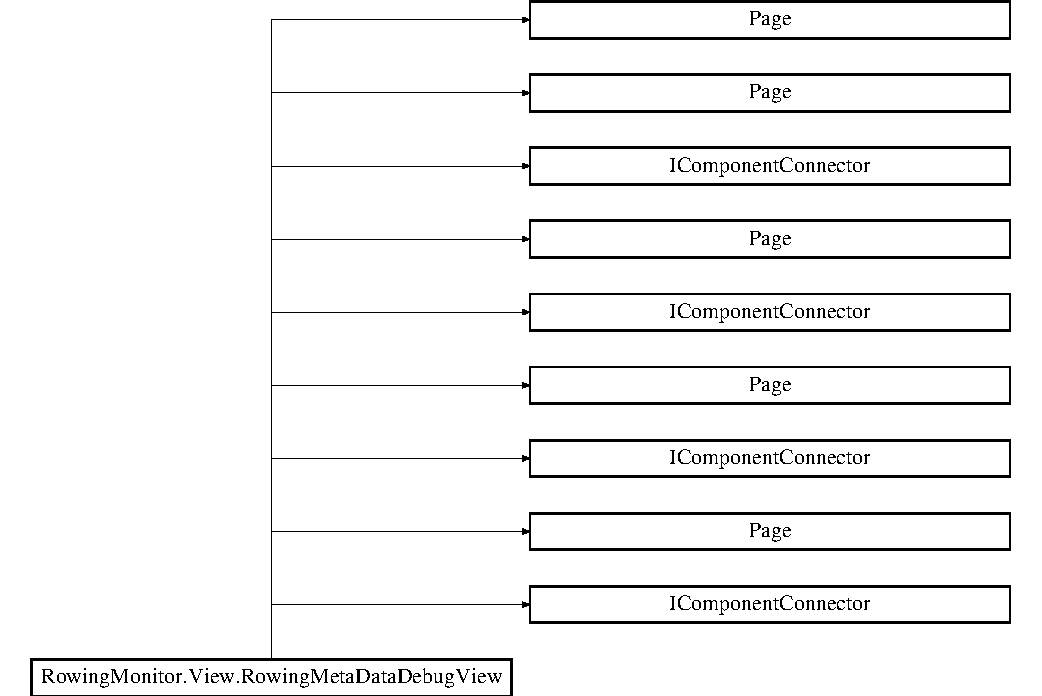
\includegraphics[height=9.333333cm]{class_rowing_monitor_1_1_view_1_1_rowing_meta_data_debug_view}
\end{center}
\end{figure}
\subsection*{Public Member Functions}
\begin{DoxyCompactItemize}
\item 
void \hyperlink{class_rowing_monitor_1_1_view_1_1_rowing_meta_data_debug_view_abc8c4176d174df5466c0503576ecc5c9}{Initialize\+Component} ()
\begin{DoxyCompactList}\small\item\em Initialize\+Component \end{DoxyCompactList}\item 
void \hyperlink{class_rowing_monitor_1_1_view_1_1_rowing_meta_data_debug_view_abc8c4176d174df5466c0503576ecc5c9}{Initialize\+Component} ()
\begin{DoxyCompactList}\small\item\em Initialize\+Component \end{DoxyCompactList}\item 
void \hyperlink{class_rowing_monitor_1_1_view_1_1_rowing_meta_data_debug_view_abc8c4176d174df5466c0503576ecc5c9}{Initialize\+Component} ()
\begin{DoxyCompactList}\small\item\em Initialize\+Component \end{DoxyCompactList}\item 
void \hyperlink{class_rowing_monitor_1_1_view_1_1_rowing_meta_data_debug_view_abc8c4176d174df5466c0503576ecc5c9}{Initialize\+Component} ()
\begin{DoxyCompactList}\small\item\em Initialize\+Component \end{DoxyCompactList}\item 
\hyperlink{class_rowing_monitor_1_1_view_1_1_rowing_meta_data_debug_view_aeffe9774bb2511a7f8217a495fc25d60}{Rowing\+Meta\+Data\+Debug\+View} ()
\end{DoxyCompactItemize}


\subsection{Detailed Description}
\hyperlink{class_rowing_monitor_1_1_view_1_1_rowing_meta_data_debug_view}{Rowing\+Meta\+Data\+Debug\+View} 

Interaktionslogik für Rowing\+Meta\+Data\+View.\+xaml 

\subsection{Constructor \& Destructor Documentation}
\mbox{\Hypertarget{class_rowing_monitor_1_1_view_1_1_rowing_meta_data_debug_view_aeffe9774bb2511a7f8217a495fc25d60}\label{class_rowing_monitor_1_1_view_1_1_rowing_meta_data_debug_view_aeffe9774bb2511a7f8217a495fc25d60}} 
\index{Rowing\+Monitor\+::\+View\+::\+Rowing\+Meta\+Data\+Debug\+View@{Rowing\+Monitor\+::\+View\+::\+Rowing\+Meta\+Data\+Debug\+View}!Rowing\+Meta\+Data\+Debug\+View@{Rowing\+Meta\+Data\+Debug\+View}}
\index{Rowing\+Meta\+Data\+Debug\+View@{Rowing\+Meta\+Data\+Debug\+View}!Rowing\+Monitor\+::\+View\+::\+Rowing\+Meta\+Data\+Debug\+View@{Rowing\+Monitor\+::\+View\+::\+Rowing\+Meta\+Data\+Debug\+View}}
\subsubsection{\texorpdfstring{Rowing\+Meta\+Data\+Debug\+View()}{RowingMetaDataDebugView()}}
{\footnotesize\ttfamily Rowing\+Monitor.\+View.\+Rowing\+Meta\+Data\+Debug\+View.\+Rowing\+Meta\+Data\+Debug\+View (\begin{DoxyParamCaption}{ }\end{DoxyParamCaption})}



\subsection{Member Function Documentation}
\mbox{\Hypertarget{class_rowing_monitor_1_1_view_1_1_rowing_meta_data_debug_view_abc8c4176d174df5466c0503576ecc5c9}\label{class_rowing_monitor_1_1_view_1_1_rowing_meta_data_debug_view_abc8c4176d174df5466c0503576ecc5c9}} 
\index{Rowing\+Monitor\+::\+View\+::\+Rowing\+Meta\+Data\+Debug\+View@{Rowing\+Monitor\+::\+View\+::\+Rowing\+Meta\+Data\+Debug\+View}!Initialize\+Component@{Initialize\+Component}}
\index{Initialize\+Component@{Initialize\+Component}!Rowing\+Monitor\+::\+View\+::\+Rowing\+Meta\+Data\+Debug\+View@{Rowing\+Monitor\+::\+View\+::\+Rowing\+Meta\+Data\+Debug\+View}}
\subsubsection{\texorpdfstring{Initialize\+Component()}{InitializeComponent()}\hspace{0.1cm}{\footnotesize\ttfamily [1/4]}}
{\footnotesize\ttfamily void Rowing\+Monitor.\+View.\+Rowing\+Meta\+Data\+Debug\+View.\+Initialize\+Component (\begin{DoxyParamCaption}{ }\end{DoxyParamCaption})}



Initialize\+Component 

\mbox{\Hypertarget{class_rowing_monitor_1_1_view_1_1_rowing_meta_data_debug_view_abc8c4176d174df5466c0503576ecc5c9}\label{class_rowing_monitor_1_1_view_1_1_rowing_meta_data_debug_view_abc8c4176d174df5466c0503576ecc5c9}} 
\index{Rowing\+Monitor\+::\+View\+::\+Rowing\+Meta\+Data\+Debug\+View@{Rowing\+Monitor\+::\+View\+::\+Rowing\+Meta\+Data\+Debug\+View}!Initialize\+Component@{Initialize\+Component}}
\index{Initialize\+Component@{Initialize\+Component}!Rowing\+Monitor\+::\+View\+::\+Rowing\+Meta\+Data\+Debug\+View@{Rowing\+Monitor\+::\+View\+::\+Rowing\+Meta\+Data\+Debug\+View}}
\subsubsection{\texorpdfstring{Initialize\+Component()}{InitializeComponent()}\hspace{0.1cm}{\footnotesize\ttfamily [2/4]}}
{\footnotesize\ttfamily void Rowing\+Monitor.\+View.\+Rowing\+Meta\+Data\+Debug\+View.\+Initialize\+Component (\begin{DoxyParamCaption}{ }\end{DoxyParamCaption})}



Initialize\+Component 

\mbox{\Hypertarget{class_rowing_monitor_1_1_view_1_1_rowing_meta_data_debug_view_abc8c4176d174df5466c0503576ecc5c9}\label{class_rowing_monitor_1_1_view_1_1_rowing_meta_data_debug_view_abc8c4176d174df5466c0503576ecc5c9}} 
\index{Rowing\+Monitor\+::\+View\+::\+Rowing\+Meta\+Data\+Debug\+View@{Rowing\+Monitor\+::\+View\+::\+Rowing\+Meta\+Data\+Debug\+View}!Initialize\+Component@{Initialize\+Component}}
\index{Initialize\+Component@{Initialize\+Component}!Rowing\+Monitor\+::\+View\+::\+Rowing\+Meta\+Data\+Debug\+View@{Rowing\+Monitor\+::\+View\+::\+Rowing\+Meta\+Data\+Debug\+View}}
\subsubsection{\texorpdfstring{Initialize\+Component()}{InitializeComponent()}\hspace{0.1cm}{\footnotesize\ttfamily [3/4]}}
{\footnotesize\ttfamily void Rowing\+Monitor.\+View.\+Rowing\+Meta\+Data\+Debug\+View.\+Initialize\+Component (\begin{DoxyParamCaption}{ }\end{DoxyParamCaption})}



Initialize\+Component 

\mbox{\Hypertarget{class_rowing_monitor_1_1_view_1_1_rowing_meta_data_debug_view_abc8c4176d174df5466c0503576ecc5c9}\label{class_rowing_monitor_1_1_view_1_1_rowing_meta_data_debug_view_abc8c4176d174df5466c0503576ecc5c9}} 
\index{Rowing\+Monitor\+::\+View\+::\+Rowing\+Meta\+Data\+Debug\+View@{Rowing\+Monitor\+::\+View\+::\+Rowing\+Meta\+Data\+Debug\+View}!Initialize\+Component@{Initialize\+Component}}
\index{Initialize\+Component@{Initialize\+Component}!Rowing\+Monitor\+::\+View\+::\+Rowing\+Meta\+Data\+Debug\+View@{Rowing\+Monitor\+::\+View\+::\+Rowing\+Meta\+Data\+Debug\+View}}
\subsubsection{\texorpdfstring{Initialize\+Component()}{InitializeComponent()}\hspace{0.1cm}{\footnotesize\ttfamily [4/4]}}
{\footnotesize\ttfamily void Rowing\+Monitor.\+View.\+Rowing\+Meta\+Data\+Debug\+View.\+Initialize\+Component (\begin{DoxyParamCaption}{ }\end{DoxyParamCaption})}



Initialize\+Component 



The documentation for this class was generated from the following files\+:\begin{DoxyCompactItemize}
\item 
obj/\+Debug/\+View/\hyperlink{_debug_2_view_2_rowing_meta_data_debug_view_8g_8cs}{Rowing\+Meta\+Data\+Debug\+View.\+g.\+cs}\item 
obj/\+Debug/\+View/\hyperlink{_debug_2_view_2_rowing_meta_data_debug_view_8g_8i_8cs}{Rowing\+Meta\+Data\+Debug\+View.\+g.\+i.\+cs}\item 
View/\hyperlink{_rowing_meta_data_debug_view_8xaml_8cs}{Rowing\+Meta\+Data\+Debug\+View.\+xaml.\+cs}\end{DoxyCompactItemize}

\hypertarget{class_rowing_monitor_1_1_view_model_1_1_rowing_meta_data_debug_view_model}{}\section{Rowing\+Monitor.\+View\+Model.\+Rowing\+Meta\+Data\+Debug\+View\+Model Class Reference}
\label{class_rowing_monitor_1_1_view_model_1_1_rowing_meta_data_debug_view_model}\index{Rowing\+Monitor.\+View\+Model.\+Rowing\+Meta\+Data\+Debug\+View\+Model@{Rowing\+Monitor.\+View\+Model.\+Rowing\+Meta\+Data\+Debug\+View\+Model}}
Inheritance diagram for Rowing\+Monitor.\+View\+Model.\+Rowing\+Meta\+Data\+Debug\+View\+Model\+:\begin{figure}[H]
\begin{center}
\leavevmode
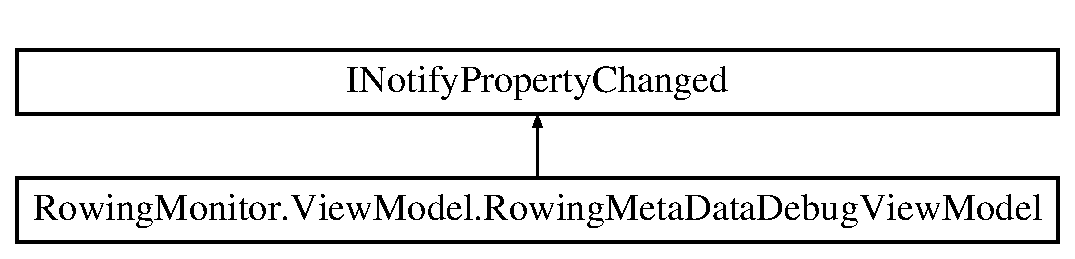
\includegraphics[height=2.000000cm]{class_rowing_monitor_1_1_view_model_1_1_rowing_meta_data_debug_view_model}
\end{center}
\end{figure}
\subsection*{Properties}
\begin{DoxyCompactItemize}
\item 
string \hyperlink{class_rowing_monitor_1_1_view_model_1_1_rowing_meta_data_debug_view_model_a122ab7c38d644175936ddf8d9e38ed5a}{Frame\+Index}\hspace{0.3cm}{\ttfamily  \mbox{[}get, set\mbox{]}}
\item 
string \hyperlink{class_rowing_monitor_1_1_view_model_1_1_rowing_meta_data_debug_view_model_a91697f56e459a585375ee42c5f40c7ed}{Session\+Time}\hspace{0.3cm}{\ttfamily  \mbox{[}get, set\mbox{]}}
\item 
string \hyperlink{class_rowing_monitor_1_1_view_model_1_1_rowing_meta_data_debug_view_model_a021415d1fc0638252b5a8a61dd5f65e0}{Stroke\+Count}\hspace{0.3cm}{\ttfamily  \mbox{[}get, set\mbox{]}}
\item 
string \hyperlink{class_rowing_monitor_1_1_view_model_1_1_rowing_meta_data_debug_view_model_a64647b5423d75ba18d9ea406770ff978}{Stroke\+Rate}\hspace{0.3cm}{\ttfamily  \mbox{[}get, set\mbox{]}}
\item 
string \hyperlink{class_rowing_monitor_1_1_view_model_1_1_rowing_meta_data_debug_view_model_a5682203c76d68ac2d357a667ec9f1a4e}{Catch\+Factor}\hspace{0.3cm}{\ttfamily  \mbox{[}get, set\mbox{]}}
\item 
string \hyperlink{class_rowing_monitor_1_1_view_model_1_1_rowing_meta_data_debug_view_model_a7cddb5fccddd903feca0984a9569f026}{Rowing\+Style\+Factor}\hspace{0.3cm}{\ttfamily  \mbox{[}get, set\mbox{]}}
\item 
string \hyperlink{class_rowing_monitor_1_1_view_model_1_1_rowing_meta_data_debug_view_model_ac65397ddf6a6af53e3f7f2a984152927}{Stroke\+Length}\hspace{0.3cm}{\ttfamily  \mbox{[}get, set\mbox{]}}
\item 
string \hyperlink{class_rowing_monitor_1_1_view_model_1_1_rowing_meta_data_debug_view_model_acbef052db26e08c4caa332017e8df8b3}{Mean\+Stroke\+Length}\hspace{0.3cm}{\ttfamily  \mbox{[}get, set\mbox{]}}
\item 
string \hyperlink{class_rowing_monitor_1_1_view_model_1_1_rowing_meta_data_debug_view_model_a9b95b1133bd4fba4a5dfbf82c7e4ea28}{Stroke\+Time}\hspace{0.3cm}{\ttfamily  \mbox{[}get, set\mbox{]}}
\item 
string \hyperlink{class_rowing_monitor_1_1_view_model_1_1_rowing_meta_data_debug_view_model_a79f3e7cbda926c9a2776bc195b60d950}{Mean\+Stroke\+Time}\hspace{0.3cm}{\ttfamily  \mbox{[}get, set\mbox{]}}
\item 
string \hyperlink{class_rowing_monitor_1_1_view_model_1_1_rowing_meta_data_debug_view_model_af3c7829aed005ae5421ee0501fd34e68}{Seat\+Travel\+Distance}\hspace{0.3cm}{\ttfamily  \mbox{[}get, set\mbox{]}}
\item 
string \hyperlink{class_rowing_monitor_1_1_view_model_1_1_rowing_meta_data_debug_view_model_a4b6c793a6db1654c7684fc6c6b71ce17}{Mean\+Seat\+Travel\+Distance}\hspace{0.3cm}{\ttfamily  \mbox{[}get, set\mbox{]}}
\item 
string \hyperlink{class_rowing_monitor_1_1_view_model_1_1_rowing_meta_data_debug_view_model_a18263a166b9e48a60aa19c1127d9eee2}{Max\+Handle\+Velocity}\hspace{0.3cm}{\ttfamily  \mbox{[}get, set\mbox{]}}
\item 
string \hyperlink{class_rowing_monitor_1_1_view_model_1_1_rowing_meta_data_debug_view_model_a1c1582da513792bc11943d02807fc720}{Mean\+Max\+Handle\+Velocity}\hspace{0.3cm}{\ttfamily  \mbox{[}get, set\mbox{]}}
\item 
string \hyperlink{class_rowing_monitor_1_1_view_model_1_1_rowing_meta_data_debug_view_model_ae78027aa407b8a37e860f223a5269eb8}{Max\+Legs\+Velocity}\hspace{0.3cm}{\ttfamily  \mbox{[}get, set\mbox{]}}
\item 
string \hyperlink{class_rowing_monitor_1_1_view_model_1_1_rowing_meta_data_debug_view_model_ad58213bfbf02d861242aa5d9c78845cd}{Mean\+Max\+Legs\+Velocity}\hspace{0.3cm}{\ttfamily  \mbox{[}get, set\mbox{]}}
\item 
string \hyperlink{class_rowing_monitor_1_1_view_model_1_1_rowing_meta_data_debug_view_model_ac5820eda650e646eac2a0adf4f88eb0d}{Max\+Arms\+Velocity}\hspace{0.3cm}{\ttfamily  \mbox{[}get, set\mbox{]}}
\item 
string \hyperlink{class_rowing_monitor_1_1_view_model_1_1_rowing_meta_data_debug_view_model_ad7dc40c4a166f7ba1a5321f35a979238}{Mean\+Max\+Arms\+Velocity}\hspace{0.3cm}{\ttfamily  \mbox{[}get, set\mbox{]}}
\item 
string \hyperlink{class_rowing_monitor_1_1_view_model_1_1_rowing_meta_data_debug_view_model_a9b29fed094b5664914c1399758bc7728}{Max\+Trunk\+Velocity}\hspace{0.3cm}{\ttfamily  \mbox{[}get, set\mbox{]}}
\item 
string \hyperlink{class_rowing_monitor_1_1_view_model_1_1_rowing_meta_data_debug_view_model_acc977e2c789b254b73a4ecbe0dc49577}{Mean\+Max\+Trunk\+Velocity}\hspace{0.3cm}{\ttfamily  \mbox{[}get, set\mbox{]}}
\item 
string \hyperlink{class_rowing_monitor_1_1_view_model_1_1_rowing_meta_data_debug_view_model_a344eb969d50db850f7e8a2ffbff96a49}{Strokes\+Per\+Minute}\hspace{0.3cm}{\ttfamily  \mbox{[}get, set\mbox{]}}
\item 
string \hyperlink{class_rowing_monitor_1_1_view_model_1_1_rowing_meta_data_debug_view_model_a42a2354e28f13dcf7ff4db58093d5604}{Trunk\+Angle}\hspace{0.3cm}{\ttfamily  \mbox{[}get, set\mbox{]}}
\item 
string \hyperlink{class_rowing_monitor_1_1_view_model_1_1_rowing_meta_data_debug_view_model_a25b04c304c6c3a5977bd2520ede1e7c3}{Max\+Catch\+Trunk\+Angle}\hspace{0.3cm}{\ttfamily  \mbox{[}get, set\mbox{]}}
\item 
string \hyperlink{class_rowing_monitor_1_1_view_model_1_1_rowing_meta_data_debug_view_model_a2fe2f846ba972b3bfa62f08d8f7e054e}{Max\+Finish\+Trunk\+Angle}\hspace{0.3cm}{\ttfamily  \mbox{[}get, set\mbox{]}}
\item 
string \hyperlink{class_rowing_monitor_1_1_view_model_1_1_rowing_meta_data_debug_view_model_ab2e80c441072f488f247942c99fa70b4}{Mean\+Catch\+Factor}\hspace{0.3cm}{\ttfamily  \mbox{[}get, set\mbox{]}}
\item 
string \hyperlink{class_rowing_monitor_1_1_view_model_1_1_rowing_meta_data_debug_view_model_a282c3663e2a5727a308e6ac8667158c8}{Mean\+Rowing\+Style\+Factor}\hspace{0.3cm}{\ttfamily  \mbox{[}get, set\mbox{]}}
\end{DoxyCompactItemize}
\subsection*{Events}
\begin{DoxyCompactItemize}
\item 
Property\+Changed\+Event\+Handler \hyperlink{class_rowing_monitor_1_1_view_model_1_1_rowing_meta_data_debug_view_model_a330fed4ef7c22c9c2f114759e07957cb}{Property\+Changed}
\end{DoxyCompactItemize}


\subsection{Property Documentation}
\mbox{\Hypertarget{class_rowing_monitor_1_1_view_model_1_1_rowing_meta_data_debug_view_model_a5682203c76d68ac2d357a667ec9f1a4e}\label{class_rowing_monitor_1_1_view_model_1_1_rowing_meta_data_debug_view_model_a5682203c76d68ac2d357a667ec9f1a4e}} 
\index{Rowing\+Monitor\+::\+View\+Model\+::\+Rowing\+Meta\+Data\+Debug\+View\+Model@{Rowing\+Monitor\+::\+View\+Model\+::\+Rowing\+Meta\+Data\+Debug\+View\+Model}!Catch\+Factor@{Catch\+Factor}}
\index{Catch\+Factor@{Catch\+Factor}!Rowing\+Monitor\+::\+View\+Model\+::\+Rowing\+Meta\+Data\+Debug\+View\+Model@{Rowing\+Monitor\+::\+View\+Model\+::\+Rowing\+Meta\+Data\+Debug\+View\+Model}}
\subsubsection{\texorpdfstring{Catch\+Factor}{CatchFactor}}
{\footnotesize\ttfamily string Rowing\+Monitor.\+View\+Model.\+Rowing\+Meta\+Data\+Debug\+View\+Model.\+Catch\+Factor\hspace{0.3cm}{\ttfamily [get]}, {\ttfamily [set]}}

\mbox{\Hypertarget{class_rowing_monitor_1_1_view_model_1_1_rowing_meta_data_debug_view_model_a122ab7c38d644175936ddf8d9e38ed5a}\label{class_rowing_monitor_1_1_view_model_1_1_rowing_meta_data_debug_view_model_a122ab7c38d644175936ddf8d9e38ed5a}} 
\index{Rowing\+Monitor\+::\+View\+Model\+::\+Rowing\+Meta\+Data\+Debug\+View\+Model@{Rowing\+Monitor\+::\+View\+Model\+::\+Rowing\+Meta\+Data\+Debug\+View\+Model}!Frame\+Index@{Frame\+Index}}
\index{Frame\+Index@{Frame\+Index}!Rowing\+Monitor\+::\+View\+Model\+::\+Rowing\+Meta\+Data\+Debug\+View\+Model@{Rowing\+Monitor\+::\+View\+Model\+::\+Rowing\+Meta\+Data\+Debug\+View\+Model}}
\subsubsection{\texorpdfstring{Frame\+Index}{FrameIndex}}
{\footnotesize\ttfamily string Rowing\+Monitor.\+View\+Model.\+Rowing\+Meta\+Data\+Debug\+View\+Model.\+Frame\+Index\hspace{0.3cm}{\ttfamily [get]}, {\ttfamily [set]}}

\mbox{\Hypertarget{class_rowing_monitor_1_1_view_model_1_1_rowing_meta_data_debug_view_model_ac5820eda650e646eac2a0adf4f88eb0d}\label{class_rowing_monitor_1_1_view_model_1_1_rowing_meta_data_debug_view_model_ac5820eda650e646eac2a0adf4f88eb0d}} 
\index{Rowing\+Monitor\+::\+View\+Model\+::\+Rowing\+Meta\+Data\+Debug\+View\+Model@{Rowing\+Monitor\+::\+View\+Model\+::\+Rowing\+Meta\+Data\+Debug\+View\+Model}!Max\+Arms\+Velocity@{Max\+Arms\+Velocity}}
\index{Max\+Arms\+Velocity@{Max\+Arms\+Velocity}!Rowing\+Monitor\+::\+View\+Model\+::\+Rowing\+Meta\+Data\+Debug\+View\+Model@{Rowing\+Monitor\+::\+View\+Model\+::\+Rowing\+Meta\+Data\+Debug\+View\+Model}}
\subsubsection{\texorpdfstring{Max\+Arms\+Velocity}{MaxArmsVelocity}}
{\footnotesize\ttfamily string Rowing\+Monitor.\+View\+Model.\+Rowing\+Meta\+Data\+Debug\+View\+Model.\+Max\+Arms\+Velocity\hspace{0.3cm}{\ttfamily [get]}, {\ttfamily [set]}}

\mbox{\Hypertarget{class_rowing_monitor_1_1_view_model_1_1_rowing_meta_data_debug_view_model_a25b04c304c6c3a5977bd2520ede1e7c3}\label{class_rowing_monitor_1_1_view_model_1_1_rowing_meta_data_debug_view_model_a25b04c304c6c3a5977bd2520ede1e7c3}} 
\index{Rowing\+Monitor\+::\+View\+Model\+::\+Rowing\+Meta\+Data\+Debug\+View\+Model@{Rowing\+Monitor\+::\+View\+Model\+::\+Rowing\+Meta\+Data\+Debug\+View\+Model}!Max\+Catch\+Trunk\+Angle@{Max\+Catch\+Trunk\+Angle}}
\index{Max\+Catch\+Trunk\+Angle@{Max\+Catch\+Trunk\+Angle}!Rowing\+Monitor\+::\+View\+Model\+::\+Rowing\+Meta\+Data\+Debug\+View\+Model@{Rowing\+Monitor\+::\+View\+Model\+::\+Rowing\+Meta\+Data\+Debug\+View\+Model}}
\subsubsection{\texorpdfstring{Max\+Catch\+Trunk\+Angle}{MaxCatchTrunkAngle}}
{\footnotesize\ttfamily string Rowing\+Monitor.\+View\+Model.\+Rowing\+Meta\+Data\+Debug\+View\+Model.\+Max\+Catch\+Trunk\+Angle\hspace{0.3cm}{\ttfamily [get]}, {\ttfamily [set]}}

\mbox{\Hypertarget{class_rowing_monitor_1_1_view_model_1_1_rowing_meta_data_debug_view_model_a2fe2f846ba972b3bfa62f08d8f7e054e}\label{class_rowing_monitor_1_1_view_model_1_1_rowing_meta_data_debug_view_model_a2fe2f846ba972b3bfa62f08d8f7e054e}} 
\index{Rowing\+Monitor\+::\+View\+Model\+::\+Rowing\+Meta\+Data\+Debug\+View\+Model@{Rowing\+Monitor\+::\+View\+Model\+::\+Rowing\+Meta\+Data\+Debug\+View\+Model}!Max\+Finish\+Trunk\+Angle@{Max\+Finish\+Trunk\+Angle}}
\index{Max\+Finish\+Trunk\+Angle@{Max\+Finish\+Trunk\+Angle}!Rowing\+Monitor\+::\+View\+Model\+::\+Rowing\+Meta\+Data\+Debug\+View\+Model@{Rowing\+Monitor\+::\+View\+Model\+::\+Rowing\+Meta\+Data\+Debug\+View\+Model}}
\subsubsection{\texorpdfstring{Max\+Finish\+Trunk\+Angle}{MaxFinishTrunkAngle}}
{\footnotesize\ttfamily string Rowing\+Monitor.\+View\+Model.\+Rowing\+Meta\+Data\+Debug\+View\+Model.\+Max\+Finish\+Trunk\+Angle\hspace{0.3cm}{\ttfamily [get]}, {\ttfamily [set]}}

\mbox{\Hypertarget{class_rowing_monitor_1_1_view_model_1_1_rowing_meta_data_debug_view_model_a18263a166b9e48a60aa19c1127d9eee2}\label{class_rowing_monitor_1_1_view_model_1_1_rowing_meta_data_debug_view_model_a18263a166b9e48a60aa19c1127d9eee2}} 
\index{Rowing\+Monitor\+::\+View\+Model\+::\+Rowing\+Meta\+Data\+Debug\+View\+Model@{Rowing\+Monitor\+::\+View\+Model\+::\+Rowing\+Meta\+Data\+Debug\+View\+Model}!Max\+Handle\+Velocity@{Max\+Handle\+Velocity}}
\index{Max\+Handle\+Velocity@{Max\+Handle\+Velocity}!Rowing\+Monitor\+::\+View\+Model\+::\+Rowing\+Meta\+Data\+Debug\+View\+Model@{Rowing\+Monitor\+::\+View\+Model\+::\+Rowing\+Meta\+Data\+Debug\+View\+Model}}
\subsubsection{\texorpdfstring{Max\+Handle\+Velocity}{MaxHandleVelocity}}
{\footnotesize\ttfamily string Rowing\+Monitor.\+View\+Model.\+Rowing\+Meta\+Data\+Debug\+View\+Model.\+Max\+Handle\+Velocity\hspace{0.3cm}{\ttfamily [get]}, {\ttfamily [set]}}

\mbox{\Hypertarget{class_rowing_monitor_1_1_view_model_1_1_rowing_meta_data_debug_view_model_ae78027aa407b8a37e860f223a5269eb8}\label{class_rowing_monitor_1_1_view_model_1_1_rowing_meta_data_debug_view_model_ae78027aa407b8a37e860f223a5269eb8}} 
\index{Rowing\+Monitor\+::\+View\+Model\+::\+Rowing\+Meta\+Data\+Debug\+View\+Model@{Rowing\+Monitor\+::\+View\+Model\+::\+Rowing\+Meta\+Data\+Debug\+View\+Model}!Max\+Legs\+Velocity@{Max\+Legs\+Velocity}}
\index{Max\+Legs\+Velocity@{Max\+Legs\+Velocity}!Rowing\+Monitor\+::\+View\+Model\+::\+Rowing\+Meta\+Data\+Debug\+View\+Model@{Rowing\+Monitor\+::\+View\+Model\+::\+Rowing\+Meta\+Data\+Debug\+View\+Model}}
\subsubsection{\texorpdfstring{Max\+Legs\+Velocity}{MaxLegsVelocity}}
{\footnotesize\ttfamily string Rowing\+Monitor.\+View\+Model.\+Rowing\+Meta\+Data\+Debug\+View\+Model.\+Max\+Legs\+Velocity\hspace{0.3cm}{\ttfamily [get]}, {\ttfamily [set]}}

\mbox{\Hypertarget{class_rowing_monitor_1_1_view_model_1_1_rowing_meta_data_debug_view_model_a9b29fed094b5664914c1399758bc7728}\label{class_rowing_monitor_1_1_view_model_1_1_rowing_meta_data_debug_view_model_a9b29fed094b5664914c1399758bc7728}} 
\index{Rowing\+Monitor\+::\+View\+Model\+::\+Rowing\+Meta\+Data\+Debug\+View\+Model@{Rowing\+Monitor\+::\+View\+Model\+::\+Rowing\+Meta\+Data\+Debug\+View\+Model}!Max\+Trunk\+Velocity@{Max\+Trunk\+Velocity}}
\index{Max\+Trunk\+Velocity@{Max\+Trunk\+Velocity}!Rowing\+Monitor\+::\+View\+Model\+::\+Rowing\+Meta\+Data\+Debug\+View\+Model@{Rowing\+Monitor\+::\+View\+Model\+::\+Rowing\+Meta\+Data\+Debug\+View\+Model}}
\subsubsection{\texorpdfstring{Max\+Trunk\+Velocity}{MaxTrunkVelocity}}
{\footnotesize\ttfamily string Rowing\+Monitor.\+View\+Model.\+Rowing\+Meta\+Data\+Debug\+View\+Model.\+Max\+Trunk\+Velocity\hspace{0.3cm}{\ttfamily [get]}, {\ttfamily [set]}}

\mbox{\Hypertarget{class_rowing_monitor_1_1_view_model_1_1_rowing_meta_data_debug_view_model_ab2e80c441072f488f247942c99fa70b4}\label{class_rowing_monitor_1_1_view_model_1_1_rowing_meta_data_debug_view_model_ab2e80c441072f488f247942c99fa70b4}} 
\index{Rowing\+Monitor\+::\+View\+Model\+::\+Rowing\+Meta\+Data\+Debug\+View\+Model@{Rowing\+Monitor\+::\+View\+Model\+::\+Rowing\+Meta\+Data\+Debug\+View\+Model}!Mean\+Catch\+Factor@{Mean\+Catch\+Factor}}
\index{Mean\+Catch\+Factor@{Mean\+Catch\+Factor}!Rowing\+Monitor\+::\+View\+Model\+::\+Rowing\+Meta\+Data\+Debug\+View\+Model@{Rowing\+Monitor\+::\+View\+Model\+::\+Rowing\+Meta\+Data\+Debug\+View\+Model}}
\subsubsection{\texorpdfstring{Mean\+Catch\+Factor}{MeanCatchFactor}}
{\footnotesize\ttfamily string Rowing\+Monitor.\+View\+Model.\+Rowing\+Meta\+Data\+Debug\+View\+Model.\+Mean\+Catch\+Factor\hspace{0.3cm}{\ttfamily [get]}, {\ttfamily [set]}}

\mbox{\Hypertarget{class_rowing_monitor_1_1_view_model_1_1_rowing_meta_data_debug_view_model_ad7dc40c4a166f7ba1a5321f35a979238}\label{class_rowing_monitor_1_1_view_model_1_1_rowing_meta_data_debug_view_model_ad7dc40c4a166f7ba1a5321f35a979238}} 
\index{Rowing\+Monitor\+::\+View\+Model\+::\+Rowing\+Meta\+Data\+Debug\+View\+Model@{Rowing\+Monitor\+::\+View\+Model\+::\+Rowing\+Meta\+Data\+Debug\+View\+Model}!Mean\+Max\+Arms\+Velocity@{Mean\+Max\+Arms\+Velocity}}
\index{Mean\+Max\+Arms\+Velocity@{Mean\+Max\+Arms\+Velocity}!Rowing\+Monitor\+::\+View\+Model\+::\+Rowing\+Meta\+Data\+Debug\+View\+Model@{Rowing\+Monitor\+::\+View\+Model\+::\+Rowing\+Meta\+Data\+Debug\+View\+Model}}
\subsubsection{\texorpdfstring{Mean\+Max\+Arms\+Velocity}{MeanMaxArmsVelocity}}
{\footnotesize\ttfamily string Rowing\+Monitor.\+View\+Model.\+Rowing\+Meta\+Data\+Debug\+View\+Model.\+Mean\+Max\+Arms\+Velocity\hspace{0.3cm}{\ttfamily [get]}, {\ttfamily [set]}}

\mbox{\Hypertarget{class_rowing_monitor_1_1_view_model_1_1_rowing_meta_data_debug_view_model_a1c1582da513792bc11943d02807fc720}\label{class_rowing_monitor_1_1_view_model_1_1_rowing_meta_data_debug_view_model_a1c1582da513792bc11943d02807fc720}} 
\index{Rowing\+Monitor\+::\+View\+Model\+::\+Rowing\+Meta\+Data\+Debug\+View\+Model@{Rowing\+Monitor\+::\+View\+Model\+::\+Rowing\+Meta\+Data\+Debug\+View\+Model}!Mean\+Max\+Handle\+Velocity@{Mean\+Max\+Handle\+Velocity}}
\index{Mean\+Max\+Handle\+Velocity@{Mean\+Max\+Handle\+Velocity}!Rowing\+Monitor\+::\+View\+Model\+::\+Rowing\+Meta\+Data\+Debug\+View\+Model@{Rowing\+Monitor\+::\+View\+Model\+::\+Rowing\+Meta\+Data\+Debug\+View\+Model}}
\subsubsection{\texorpdfstring{Mean\+Max\+Handle\+Velocity}{MeanMaxHandleVelocity}}
{\footnotesize\ttfamily string Rowing\+Monitor.\+View\+Model.\+Rowing\+Meta\+Data\+Debug\+View\+Model.\+Mean\+Max\+Handle\+Velocity\hspace{0.3cm}{\ttfamily [get]}, {\ttfamily [set]}}

\mbox{\Hypertarget{class_rowing_monitor_1_1_view_model_1_1_rowing_meta_data_debug_view_model_ad58213bfbf02d861242aa5d9c78845cd}\label{class_rowing_monitor_1_1_view_model_1_1_rowing_meta_data_debug_view_model_ad58213bfbf02d861242aa5d9c78845cd}} 
\index{Rowing\+Monitor\+::\+View\+Model\+::\+Rowing\+Meta\+Data\+Debug\+View\+Model@{Rowing\+Monitor\+::\+View\+Model\+::\+Rowing\+Meta\+Data\+Debug\+View\+Model}!Mean\+Max\+Legs\+Velocity@{Mean\+Max\+Legs\+Velocity}}
\index{Mean\+Max\+Legs\+Velocity@{Mean\+Max\+Legs\+Velocity}!Rowing\+Monitor\+::\+View\+Model\+::\+Rowing\+Meta\+Data\+Debug\+View\+Model@{Rowing\+Monitor\+::\+View\+Model\+::\+Rowing\+Meta\+Data\+Debug\+View\+Model}}
\subsubsection{\texorpdfstring{Mean\+Max\+Legs\+Velocity}{MeanMaxLegsVelocity}}
{\footnotesize\ttfamily string Rowing\+Monitor.\+View\+Model.\+Rowing\+Meta\+Data\+Debug\+View\+Model.\+Mean\+Max\+Legs\+Velocity\hspace{0.3cm}{\ttfamily [get]}, {\ttfamily [set]}}

\mbox{\Hypertarget{class_rowing_monitor_1_1_view_model_1_1_rowing_meta_data_debug_view_model_acc977e2c789b254b73a4ecbe0dc49577}\label{class_rowing_monitor_1_1_view_model_1_1_rowing_meta_data_debug_view_model_acc977e2c789b254b73a4ecbe0dc49577}} 
\index{Rowing\+Monitor\+::\+View\+Model\+::\+Rowing\+Meta\+Data\+Debug\+View\+Model@{Rowing\+Monitor\+::\+View\+Model\+::\+Rowing\+Meta\+Data\+Debug\+View\+Model}!Mean\+Max\+Trunk\+Velocity@{Mean\+Max\+Trunk\+Velocity}}
\index{Mean\+Max\+Trunk\+Velocity@{Mean\+Max\+Trunk\+Velocity}!Rowing\+Monitor\+::\+View\+Model\+::\+Rowing\+Meta\+Data\+Debug\+View\+Model@{Rowing\+Monitor\+::\+View\+Model\+::\+Rowing\+Meta\+Data\+Debug\+View\+Model}}
\subsubsection{\texorpdfstring{Mean\+Max\+Trunk\+Velocity}{MeanMaxTrunkVelocity}}
{\footnotesize\ttfamily string Rowing\+Monitor.\+View\+Model.\+Rowing\+Meta\+Data\+Debug\+View\+Model.\+Mean\+Max\+Trunk\+Velocity\hspace{0.3cm}{\ttfamily [get]}, {\ttfamily [set]}}

\mbox{\Hypertarget{class_rowing_monitor_1_1_view_model_1_1_rowing_meta_data_debug_view_model_a282c3663e2a5727a308e6ac8667158c8}\label{class_rowing_monitor_1_1_view_model_1_1_rowing_meta_data_debug_view_model_a282c3663e2a5727a308e6ac8667158c8}} 
\index{Rowing\+Monitor\+::\+View\+Model\+::\+Rowing\+Meta\+Data\+Debug\+View\+Model@{Rowing\+Monitor\+::\+View\+Model\+::\+Rowing\+Meta\+Data\+Debug\+View\+Model}!Mean\+Rowing\+Style\+Factor@{Mean\+Rowing\+Style\+Factor}}
\index{Mean\+Rowing\+Style\+Factor@{Mean\+Rowing\+Style\+Factor}!Rowing\+Monitor\+::\+View\+Model\+::\+Rowing\+Meta\+Data\+Debug\+View\+Model@{Rowing\+Monitor\+::\+View\+Model\+::\+Rowing\+Meta\+Data\+Debug\+View\+Model}}
\subsubsection{\texorpdfstring{Mean\+Rowing\+Style\+Factor}{MeanRowingStyleFactor}}
{\footnotesize\ttfamily string Rowing\+Monitor.\+View\+Model.\+Rowing\+Meta\+Data\+Debug\+View\+Model.\+Mean\+Rowing\+Style\+Factor\hspace{0.3cm}{\ttfamily [get]}, {\ttfamily [set]}}

\mbox{\Hypertarget{class_rowing_monitor_1_1_view_model_1_1_rowing_meta_data_debug_view_model_a4b6c793a6db1654c7684fc6c6b71ce17}\label{class_rowing_monitor_1_1_view_model_1_1_rowing_meta_data_debug_view_model_a4b6c793a6db1654c7684fc6c6b71ce17}} 
\index{Rowing\+Monitor\+::\+View\+Model\+::\+Rowing\+Meta\+Data\+Debug\+View\+Model@{Rowing\+Monitor\+::\+View\+Model\+::\+Rowing\+Meta\+Data\+Debug\+View\+Model}!Mean\+Seat\+Travel\+Distance@{Mean\+Seat\+Travel\+Distance}}
\index{Mean\+Seat\+Travel\+Distance@{Mean\+Seat\+Travel\+Distance}!Rowing\+Monitor\+::\+View\+Model\+::\+Rowing\+Meta\+Data\+Debug\+View\+Model@{Rowing\+Monitor\+::\+View\+Model\+::\+Rowing\+Meta\+Data\+Debug\+View\+Model}}
\subsubsection{\texorpdfstring{Mean\+Seat\+Travel\+Distance}{MeanSeatTravelDistance}}
{\footnotesize\ttfamily string Rowing\+Monitor.\+View\+Model.\+Rowing\+Meta\+Data\+Debug\+View\+Model.\+Mean\+Seat\+Travel\+Distance\hspace{0.3cm}{\ttfamily [get]}, {\ttfamily [set]}}

\mbox{\Hypertarget{class_rowing_monitor_1_1_view_model_1_1_rowing_meta_data_debug_view_model_acbef052db26e08c4caa332017e8df8b3}\label{class_rowing_monitor_1_1_view_model_1_1_rowing_meta_data_debug_view_model_acbef052db26e08c4caa332017e8df8b3}} 
\index{Rowing\+Monitor\+::\+View\+Model\+::\+Rowing\+Meta\+Data\+Debug\+View\+Model@{Rowing\+Monitor\+::\+View\+Model\+::\+Rowing\+Meta\+Data\+Debug\+View\+Model}!Mean\+Stroke\+Length@{Mean\+Stroke\+Length}}
\index{Mean\+Stroke\+Length@{Mean\+Stroke\+Length}!Rowing\+Monitor\+::\+View\+Model\+::\+Rowing\+Meta\+Data\+Debug\+View\+Model@{Rowing\+Monitor\+::\+View\+Model\+::\+Rowing\+Meta\+Data\+Debug\+View\+Model}}
\subsubsection{\texorpdfstring{Mean\+Stroke\+Length}{MeanStrokeLength}}
{\footnotesize\ttfamily string Rowing\+Monitor.\+View\+Model.\+Rowing\+Meta\+Data\+Debug\+View\+Model.\+Mean\+Stroke\+Length\hspace{0.3cm}{\ttfamily [get]}, {\ttfamily [set]}}

\mbox{\Hypertarget{class_rowing_monitor_1_1_view_model_1_1_rowing_meta_data_debug_view_model_a79f3e7cbda926c9a2776bc195b60d950}\label{class_rowing_monitor_1_1_view_model_1_1_rowing_meta_data_debug_view_model_a79f3e7cbda926c9a2776bc195b60d950}} 
\index{Rowing\+Monitor\+::\+View\+Model\+::\+Rowing\+Meta\+Data\+Debug\+View\+Model@{Rowing\+Monitor\+::\+View\+Model\+::\+Rowing\+Meta\+Data\+Debug\+View\+Model}!Mean\+Stroke\+Time@{Mean\+Stroke\+Time}}
\index{Mean\+Stroke\+Time@{Mean\+Stroke\+Time}!Rowing\+Monitor\+::\+View\+Model\+::\+Rowing\+Meta\+Data\+Debug\+View\+Model@{Rowing\+Monitor\+::\+View\+Model\+::\+Rowing\+Meta\+Data\+Debug\+View\+Model}}
\subsubsection{\texorpdfstring{Mean\+Stroke\+Time}{MeanStrokeTime}}
{\footnotesize\ttfamily string Rowing\+Monitor.\+View\+Model.\+Rowing\+Meta\+Data\+Debug\+View\+Model.\+Mean\+Stroke\+Time\hspace{0.3cm}{\ttfamily [get]}, {\ttfamily [set]}}

\mbox{\Hypertarget{class_rowing_monitor_1_1_view_model_1_1_rowing_meta_data_debug_view_model_a7cddb5fccddd903feca0984a9569f026}\label{class_rowing_monitor_1_1_view_model_1_1_rowing_meta_data_debug_view_model_a7cddb5fccddd903feca0984a9569f026}} 
\index{Rowing\+Monitor\+::\+View\+Model\+::\+Rowing\+Meta\+Data\+Debug\+View\+Model@{Rowing\+Monitor\+::\+View\+Model\+::\+Rowing\+Meta\+Data\+Debug\+View\+Model}!Rowing\+Style\+Factor@{Rowing\+Style\+Factor}}
\index{Rowing\+Style\+Factor@{Rowing\+Style\+Factor}!Rowing\+Monitor\+::\+View\+Model\+::\+Rowing\+Meta\+Data\+Debug\+View\+Model@{Rowing\+Monitor\+::\+View\+Model\+::\+Rowing\+Meta\+Data\+Debug\+View\+Model}}
\subsubsection{\texorpdfstring{Rowing\+Style\+Factor}{RowingStyleFactor}}
{\footnotesize\ttfamily string Rowing\+Monitor.\+View\+Model.\+Rowing\+Meta\+Data\+Debug\+View\+Model.\+Rowing\+Style\+Factor\hspace{0.3cm}{\ttfamily [get]}, {\ttfamily [set]}}

\mbox{\Hypertarget{class_rowing_monitor_1_1_view_model_1_1_rowing_meta_data_debug_view_model_af3c7829aed005ae5421ee0501fd34e68}\label{class_rowing_monitor_1_1_view_model_1_1_rowing_meta_data_debug_view_model_af3c7829aed005ae5421ee0501fd34e68}} 
\index{Rowing\+Monitor\+::\+View\+Model\+::\+Rowing\+Meta\+Data\+Debug\+View\+Model@{Rowing\+Monitor\+::\+View\+Model\+::\+Rowing\+Meta\+Data\+Debug\+View\+Model}!Seat\+Travel\+Distance@{Seat\+Travel\+Distance}}
\index{Seat\+Travel\+Distance@{Seat\+Travel\+Distance}!Rowing\+Monitor\+::\+View\+Model\+::\+Rowing\+Meta\+Data\+Debug\+View\+Model@{Rowing\+Monitor\+::\+View\+Model\+::\+Rowing\+Meta\+Data\+Debug\+View\+Model}}
\subsubsection{\texorpdfstring{Seat\+Travel\+Distance}{SeatTravelDistance}}
{\footnotesize\ttfamily string Rowing\+Monitor.\+View\+Model.\+Rowing\+Meta\+Data\+Debug\+View\+Model.\+Seat\+Travel\+Distance\hspace{0.3cm}{\ttfamily [get]}, {\ttfamily [set]}}

\mbox{\Hypertarget{class_rowing_monitor_1_1_view_model_1_1_rowing_meta_data_debug_view_model_a91697f56e459a585375ee42c5f40c7ed}\label{class_rowing_monitor_1_1_view_model_1_1_rowing_meta_data_debug_view_model_a91697f56e459a585375ee42c5f40c7ed}} 
\index{Rowing\+Monitor\+::\+View\+Model\+::\+Rowing\+Meta\+Data\+Debug\+View\+Model@{Rowing\+Monitor\+::\+View\+Model\+::\+Rowing\+Meta\+Data\+Debug\+View\+Model}!Session\+Time@{Session\+Time}}
\index{Session\+Time@{Session\+Time}!Rowing\+Monitor\+::\+View\+Model\+::\+Rowing\+Meta\+Data\+Debug\+View\+Model@{Rowing\+Monitor\+::\+View\+Model\+::\+Rowing\+Meta\+Data\+Debug\+View\+Model}}
\subsubsection{\texorpdfstring{Session\+Time}{SessionTime}}
{\footnotesize\ttfamily string Rowing\+Monitor.\+View\+Model.\+Rowing\+Meta\+Data\+Debug\+View\+Model.\+Session\+Time\hspace{0.3cm}{\ttfamily [get]}, {\ttfamily [set]}}

\mbox{\Hypertarget{class_rowing_monitor_1_1_view_model_1_1_rowing_meta_data_debug_view_model_a021415d1fc0638252b5a8a61dd5f65e0}\label{class_rowing_monitor_1_1_view_model_1_1_rowing_meta_data_debug_view_model_a021415d1fc0638252b5a8a61dd5f65e0}} 
\index{Rowing\+Monitor\+::\+View\+Model\+::\+Rowing\+Meta\+Data\+Debug\+View\+Model@{Rowing\+Monitor\+::\+View\+Model\+::\+Rowing\+Meta\+Data\+Debug\+View\+Model}!Stroke\+Count@{Stroke\+Count}}
\index{Stroke\+Count@{Stroke\+Count}!Rowing\+Monitor\+::\+View\+Model\+::\+Rowing\+Meta\+Data\+Debug\+View\+Model@{Rowing\+Monitor\+::\+View\+Model\+::\+Rowing\+Meta\+Data\+Debug\+View\+Model}}
\subsubsection{\texorpdfstring{Stroke\+Count}{StrokeCount}}
{\footnotesize\ttfamily string Rowing\+Monitor.\+View\+Model.\+Rowing\+Meta\+Data\+Debug\+View\+Model.\+Stroke\+Count\hspace{0.3cm}{\ttfamily [get]}, {\ttfamily [set]}}

\mbox{\Hypertarget{class_rowing_monitor_1_1_view_model_1_1_rowing_meta_data_debug_view_model_ac65397ddf6a6af53e3f7f2a984152927}\label{class_rowing_monitor_1_1_view_model_1_1_rowing_meta_data_debug_view_model_ac65397ddf6a6af53e3f7f2a984152927}} 
\index{Rowing\+Monitor\+::\+View\+Model\+::\+Rowing\+Meta\+Data\+Debug\+View\+Model@{Rowing\+Monitor\+::\+View\+Model\+::\+Rowing\+Meta\+Data\+Debug\+View\+Model}!Stroke\+Length@{Stroke\+Length}}
\index{Stroke\+Length@{Stroke\+Length}!Rowing\+Monitor\+::\+View\+Model\+::\+Rowing\+Meta\+Data\+Debug\+View\+Model@{Rowing\+Monitor\+::\+View\+Model\+::\+Rowing\+Meta\+Data\+Debug\+View\+Model}}
\subsubsection{\texorpdfstring{Stroke\+Length}{StrokeLength}}
{\footnotesize\ttfamily string Rowing\+Monitor.\+View\+Model.\+Rowing\+Meta\+Data\+Debug\+View\+Model.\+Stroke\+Length\hspace{0.3cm}{\ttfamily [get]}, {\ttfamily [set]}}

\mbox{\Hypertarget{class_rowing_monitor_1_1_view_model_1_1_rowing_meta_data_debug_view_model_a64647b5423d75ba18d9ea406770ff978}\label{class_rowing_monitor_1_1_view_model_1_1_rowing_meta_data_debug_view_model_a64647b5423d75ba18d9ea406770ff978}} 
\index{Rowing\+Monitor\+::\+View\+Model\+::\+Rowing\+Meta\+Data\+Debug\+View\+Model@{Rowing\+Monitor\+::\+View\+Model\+::\+Rowing\+Meta\+Data\+Debug\+View\+Model}!Stroke\+Rate@{Stroke\+Rate}}
\index{Stroke\+Rate@{Stroke\+Rate}!Rowing\+Monitor\+::\+View\+Model\+::\+Rowing\+Meta\+Data\+Debug\+View\+Model@{Rowing\+Monitor\+::\+View\+Model\+::\+Rowing\+Meta\+Data\+Debug\+View\+Model}}
\subsubsection{\texorpdfstring{Stroke\+Rate}{StrokeRate}}
{\footnotesize\ttfamily string Rowing\+Monitor.\+View\+Model.\+Rowing\+Meta\+Data\+Debug\+View\+Model.\+Stroke\+Rate\hspace{0.3cm}{\ttfamily [get]}, {\ttfamily [set]}}

\mbox{\Hypertarget{class_rowing_monitor_1_1_view_model_1_1_rowing_meta_data_debug_view_model_a344eb969d50db850f7e8a2ffbff96a49}\label{class_rowing_monitor_1_1_view_model_1_1_rowing_meta_data_debug_view_model_a344eb969d50db850f7e8a2ffbff96a49}} 
\index{Rowing\+Monitor\+::\+View\+Model\+::\+Rowing\+Meta\+Data\+Debug\+View\+Model@{Rowing\+Monitor\+::\+View\+Model\+::\+Rowing\+Meta\+Data\+Debug\+View\+Model}!Strokes\+Per\+Minute@{Strokes\+Per\+Minute}}
\index{Strokes\+Per\+Minute@{Strokes\+Per\+Minute}!Rowing\+Monitor\+::\+View\+Model\+::\+Rowing\+Meta\+Data\+Debug\+View\+Model@{Rowing\+Monitor\+::\+View\+Model\+::\+Rowing\+Meta\+Data\+Debug\+View\+Model}}
\subsubsection{\texorpdfstring{Strokes\+Per\+Minute}{StrokesPerMinute}}
{\footnotesize\ttfamily string Rowing\+Monitor.\+View\+Model.\+Rowing\+Meta\+Data\+Debug\+View\+Model.\+Strokes\+Per\+Minute\hspace{0.3cm}{\ttfamily [get]}, {\ttfamily [set]}}

\mbox{\Hypertarget{class_rowing_monitor_1_1_view_model_1_1_rowing_meta_data_debug_view_model_a9b95b1133bd4fba4a5dfbf82c7e4ea28}\label{class_rowing_monitor_1_1_view_model_1_1_rowing_meta_data_debug_view_model_a9b95b1133bd4fba4a5dfbf82c7e4ea28}} 
\index{Rowing\+Monitor\+::\+View\+Model\+::\+Rowing\+Meta\+Data\+Debug\+View\+Model@{Rowing\+Monitor\+::\+View\+Model\+::\+Rowing\+Meta\+Data\+Debug\+View\+Model}!Stroke\+Time@{Stroke\+Time}}
\index{Stroke\+Time@{Stroke\+Time}!Rowing\+Monitor\+::\+View\+Model\+::\+Rowing\+Meta\+Data\+Debug\+View\+Model@{Rowing\+Monitor\+::\+View\+Model\+::\+Rowing\+Meta\+Data\+Debug\+View\+Model}}
\subsubsection{\texorpdfstring{Stroke\+Time}{StrokeTime}}
{\footnotesize\ttfamily string Rowing\+Monitor.\+View\+Model.\+Rowing\+Meta\+Data\+Debug\+View\+Model.\+Stroke\+Time\hspace{0.3cm}{\ttfamily [get]}, {\ttfamily [set]}}

\mbox{\Hypertarget{class_rowing_monitor_1_1_view_model_1_1_rowing_meta_data_debug_view_model_a42a2354e28f13dcf7ff4db58093d5604}\label{class_rowing_monitor_1_1_view_model_1_1_rowing_meta_data_debug_view_model_a42a2354e28f13dcf7ff4db58093d5604}} 
\index{Rowing\+Monitor\+::\+View\+Model\+::\+Rowing\+Meta\+Data\+Debug\+View\+Model@{Rowing\+Monitor\+::\+View\+Model\+::\+Rowing\+Meta\+Data\+Debug\+View\+Model}!Trunk\+Angle@{Trunk\+Angle}}
\index{Trunk\+Angle@{Trunk\+Angle}!Rowing\+Monitor\+::\+View\+Model\+::\+Rowing\+Meta\+Data\+Debug\+View\+Model@{Rowing\+Monitor\+::\+View\+Model\+::\+Rowing\+Meta\+Data\+Debug\+View\+Model}}
\subsubsection{\texorpdfstring{Trunk\+Angle}{TrunkAngle}}
{\footnotesize\ttfamily string Rowing\+Monitor.\+View\+Model.\+Rowing\+Meta\+Data\+Debug\+View\+Model.\+Trunk\+Angle\hspace{0.3cm}{\ttfamily [get]}, {\ttfamily [set]}}



\subsection{Event Documentation}
\mbox{\Hypertarget{class_rowing_monitor_1_1_view_model_1_1_rowing_meta_data_debug_view_model_a330fed4ef7c22c9c2f114759e07957cb}\label{class_rowing_monitor_1_1_view_model_1_1_rowing_meta_data_debug_view_model_a330fed4ef7c22c9c2f114759e07957cb}} 
\index{Rowing\+Monitor\+::\+View\+Model\+::\+Rowing\+Meta\+Data\+Debug\+View\+Model@{Rowing\+Monitor\+::\+View\+Model\+::\+Rowing\+Meta\+Data\+Debug\+View\+Model}!Property\+Changed@{Property\+Changed}}
\index{Property\+Changed@{Property\+Changed}!Rowing\+Monitor\+::\+View\+Model\+::\+Rowing\+Meta\+Data\+Debug\+View\+Model@{Rowing\+Monitor\+::\+View\+Model\+::\+Rowing\+Meta\+Data\+Debug\+View\+Model}}
\subsubsection{\texorpdfstring{Property\+Changed}{PropertyChanged}}
{\footnotesize\ttfamily Property\+Changed\+Event\+Handler Rowing\+Monitor.\+View\+Model.\+Rowing\+Meta\+Data\+Debug\+View\+Model.\+Property\+Changed}



The documentation for this class was generated from the following file\+:\begin{DoxyCompactItemize}
\item 
View\+Model/\hyperlink{_rowing_meta_data_debug_view_model_8cs}{Rowing\+Meta\+Data\+Debug\+View\+Model.\+cs}\end{DoxyCompactItemize}

\hypertarget{class_rowing_monitor_1_1_model_1_1_util_1_1_rowing_meta_data_handler}{}\section{Rowing\+Monitor.\+Model.\+Util.\+Rowing\+Meta\+Data\+Handler Class Reference}
\label{class_rowing_monitor_1_1_model_1_1_util_1_1_rowing_meta_data_handler}\index{Rowing\+Monitor.\+Model.\+Util.\+Rowing\+Meta\+Data\+Handler@{Rowing\+Monitor.\+Model.\+Util.\+Rowing\+Meta\+Data\+Handler}}


The documentation for this class was generated from the following file\+:\begin{DoxyCompactItemize}
\item 
Model/\+Util/\hyperlink{_rowing_meta_data_handler_8cs}{Rowing\+Meta\+Data\+Handler.\+cs}\end{DoxyCompactItemize}

\hypertarget{class_rowing_monitor_1_1_view_1_1_rowing_meta_data_view}{}\section{Rowing\+Monitor.\+View.\+Rowing\+Meta\+Data\+View Class Reference}
\label{class_rowing_monitor_1_1_view_1_1_rowing_meta_data_view}\index{Rowing\+Monitor.\+View.\+Rowing\+Meta\+Data\+View@{Rowing\+Monitor.\+View.\+Rowing\+Meta\+Data\+View}}


\hyperlink{class_rowing_monitor_1_1_view_1_1_rowing_meta_data_view}{Rowing\+Meta\+Data\+View}  


Inheritance diagram for Rowing\+Monitor.\+View.\+Rowing\+Meta\+Data\+View\+:\begin{figure}[H]
\begin{center}
\leavevmode
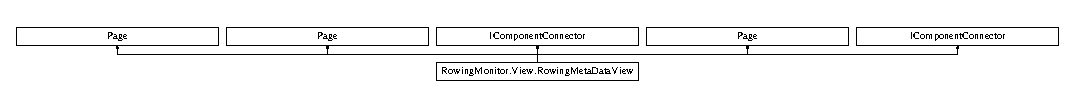
\includegraphics[height=0.851711cm]{class_rowing_monitor_1_1_view_1_1_rowing_meta_data_view}
\end{center}
\end{figure}
\subsection*{Public Member Functions}
\begin{DoxyCompactItemize}
\item 
void \hyperlink{class_rowing_monitor_1_1_view_1_1_rowing_meta_data_view_a3d445692062269ce977812772d5c4d97}{Initialize\+Component} ()
\begin{DoxyCompactList}\small\item\em Initialize\+Component \end{DoxyCompactList}\item 
void \hyperlink{class_rowing_monitor_1_1_view_1_1_rowing_meta_data_view_a3d445692062269ce977812772d5c4d97}{Initialize\+Component} ()
\begin{DoxyCompactList}\small\item\em Initialize\+Component \end{DoxyCompactList}\item 
\hyperlink{class_rowing_monitor_1_1_view_1_1_rowing_meta_data_view_a0d89dc0f01cc88aed475f15a5aff4059}{Rowing\+Meta\+Data\+View} ()
\end{DoxyCompactItemize}


\subsection{Detailed Description}
\hyperlink{class_rowing_monitor_1_1_view_1_1_rowing_meta_data_view}{Rowing\+Meta\+Data\+View} 

Interaktionslogik für Rowing\+Meta\+Data\+View.\+xaml 

\subsection{Constructor \& Destructor Documentation}
\mbox{\Hypertarget{class_rowing_monitor_1_1_view_1_1_rowing_meta_data_view_a0d89dc0f01cc88aed475f15a5aff4059}\label{class_rowing_monitor_1_1_view_1_1_rowing_meta_data_view_a0d89dc0f01cc88aed475f15a5aff4059}} 
\index{Rowing\+Monitor\+::\+View\+::\+Rowing\+Meta\+Data\+View@{Rowing\+Monitor\+::\+View\+::\+Rowing\+Meta\+Data\+View}!Rowing\+Meta\+Data\+View@{Rowing\+Meta\+Data\+View}}
\index{Rowing\+Meta\+Data\+View@{Rowing\+Meta\+Data\+View}!Rowing\+Monitor\+::\+View\+::\+Rowing\+Meta\+Data\+View@{Rowing\+Monitor\+::\+View\+::\+Rowing\+Meta\+Data\+View}}
\subsubsection{\texorpdfstring{Rowing\+Meta\+Data\+View()}{RowingMetaDataView()}}
{\footnotesize\ttfamily Rowing\+Monitor.\+View.\+Rowing\+Meta\+Data\+View.\+Rowing\+Meta\+Data\+View (\begin{DoxyParamCaption}{ }\end{DoxyParamCaption})}



\subsection{Member Function Documentation}
\mbox{\Hypertarget{class_rowing_monitor_1_1_view_1_1_rowing_meta_data_view_a3d445692062269ce977812772d5c4d97}\label{class_rowing_monitor_1_1_view_1_1_rowing_meta_data_view_a3d445692062269ce977812772d5c4d97}} 
\index{Rowing\+Monitor\+::\+View\+::\+Rowing\+Meta\+Data\+View@{Rowing\+Monitor\+::\+View\+::\+Rowing\+Meta\+Data\+View}!Initialize\+Component@{Initialize\+Component}}
\index{Initialize\+Component@{Initialize\+Component}!Rowing\+Monitor\+::\+View\+::\+Rowing\+Meta\+Data\+View@{Rowing\+Monitor\+::\+View\+::\+Rowing\+Meta\+Data\+View}}
\subsubsection{\texorpdfstring{Initialize\+Component()}{InitializeComponent()}\hspace{0.1cm}{\footnotesize\ttfamily [1/2]}}
{\footnotesize\ttfamily void Rowing\+Monitor.\+View.\+Rowing\+Meta\+Data\+View.\+Initialize\+Component (\begin{DoxyParamCaption}{ }\end{DoxyParamCaption})}



Initialize\+Component 

\mbox{\Hypertarget{class_rowing_monitor_1_1_view_1_1_rowing_meta_data_view_a3d445692062269ce977812772d5c4d97}\label{class_rowing_monitor_1_1_view_1_1_rowing_meta_data_view_a3d445692062269ce977812772d5c4d97}} 
\index{Rowing\+Monitor\+::\+View\+::\+Rowing\+Meta\+Data\+View@{Rowing\+Monitor\+::\+View\+::\+Rowing\+Meta\+Data\+View}!Initialize\+Component@{Initialize\+Component}}
\index{Initialize\+Component@{Initialize\+Component}!Rowing\+Monitor\+::\+View\+::\+Rowing\+Meta\+Data\+View@{Rowing\+Monitor\+::\+View\+::\+Rowing\+Meta\+Data\+View}}
\subsubsection{\texorpdfstring{Initialize\+Component()}{InitializeComponent()}\hspace{0.1cm}{\footnotesize\ttfamily [2/2]}}
{\footnotesize\ttfamily void Rowing\+Monitor.\+View.\+Rowing\+Meta\+Data\+View.\+Initialize\+Component (\begin{DoxyParamCaption}{ }\end{DoxyParamCaption})}



Initialize\+Component 



The documentation for this class was generated from the following files\+:\begin{DoxyCompactItemize}
\item 
obj/\+Debug/\+View/\hyperlink{_rowing_meta_data_view_8g_8cs}{Rowing\+Meta\+Data\+View.\+g.\+cs}\item 
obj/\+Debug/\+View/\hyperlink{_rowing_meta_data_view_8g_8i_8cs}{Rowing\+Meta\+Data\+View.\+g.\+i.\+cs}\item 
View/\hyperlink{_rowing_meta_data_view_8xaml_8cs}{Rowing\+Meta\+Data\+View.\+xaml.\+cs}\end{DoxyCompactItemize}

\hypertarget{class_rowing_monitor_1_1_model_1_1_pipeline_1_1_rowing_meta_data_widgets_display}{}\section{Rowing\+Monitor.\+Model.\+Pipeline.\+Rowing\+Meta\+Data\+Widgets\+Display Class Reference}
\label{class_rowing_monitor_1_1_model_1_1_pipeline_1_1_rowing_meta_data_widgets_display}\index{Rowing\+Monitor.\+Model.\+Pipeline.\+Rowing\+Meta\+Data\+Widgets\+Display@{Rowing\+Monitor.\+Model.\+Pipeline.\+Rowing\+Meta\+Data\+Widgets\+Display}}
\subsection*{Public Member Functions}
\begin{DoxyCompactItemize}
\item 
\hyperlink{class_rowing_monitor_1_1_model_1_1_pipeline_1_1_rowing_meta_data_widgets_display_a7ed8966ffb6bb02591cfa8f770ebb979}{Rowing\+Meta\+Data\+Widgets\+Display} ()
\item 
void \hyperlink{class_rowing_monitor_1_1_model_1_1_pipeline_1_1_rowing_meta_data_widgets_display_a09e7f318f293d98ad7d18949aea1f47a}{Render} ()
\end{DoxyCompactItemize}
\subsection*{Properties}
\begin{DoxyCompactItemize}
\item 
Action\+Block$<$ \hyperlink{struct_rowing_monitor_1_1_model_1_1_util_1_1_rowing_meta_data}{Rowing\+Meta\+Data} $>$ \hyperlink{class_rowing_monitor_1_1_model_1_1_pipeline_1_1_rowing_meta_data_widgets_display_a283a70144d7d3d3c495d3fd987410bc8}{Input}\hspace{0.3cm}{\ttfamily  \mbox{[}get, set\mbox{]}}
\item 
\hyperlink{class_rowing_monitor_1_1_view_1_1_rowing_meta_data_widgets_view}{Rowing\+Meta\+Data\+Widgets\+View} \hyperlink{class_rowing_monitor_1_1_model_1_1_pipeline_1_1_rowing_meta_data_widgets_display_ab88d3d1b60306b8e0b02df376f613d07}{View}\hspace{0.3cm}{\ttfamily  \mbox{[}get, set\mbox{]}}
\end{DoxyCompactItemize}


\subsection{Constructor \& Destructor Documentation}
\mbox{\Hypertarget{class_rowing_monitor_1_1_model_1_1_pipeline_1_1_rowing_meta_data_widgets_display_a7ed8966ffb6bb02591cfa8f770ebb979}\label{class_rowing_monitor_1_1_model_1_1_pipeline_1_1_rowing_meta_data_widgets_display_a7ed8966ffb6bb02591cfa8f770ebb979}} 
\index{Rowing\+Monitor\+::\+Model\+::\+Pipeline\+::\+Rowing\+Meta\+Data\+Widgets\+Display@{Rowing\+Monitor\+::\+Model\+::\+Pipeline\+::\+Rowing\+Meta\+Data\+Widgets\+Display}!Rowing\+Meta\+Data\+Widgets\+Display@{Rowing\+Meta\+Data\+Widgets\+Display}}
\index{Rowing\+Meta\+Data\+Widgets\+Display@{Rowing\+Meta\+Data\+Widgets\+Display}!Rowing\+Monitor\+::\+Model\+::\+Pipeline\+::\+Rowing\+Meta\+Data\+Widgets\+Display@{Rowing\+Monitor\+::\+Model\+::\+Pipeline\+::\+Rowing\+Meta\+Data\+Widgets\+Display}}
\subsubsection{\texorpdfstring{Rowing\+Meta\+Data\+Widgets\+Display()}{RowingMetaDataWidgetsDisplay()}}
{\footnotesize\ttfamily Rowing\+Monitor.\+Model.\+Pipeline.\+Rowing\+Meta\+Data\+Widgets\+Display.\+Rowing\+Meta\+Data\+Widgets\+Display (\begin{DoxyParamCaption}{ }\end{DoxyParamCaption})}



\subsection{Member Function Documentation}
\mbox{\Hypertarget{class_rowing_monitor_1_1_model_1_1_pipeline_1_1_rowing_meta_data_widgets_display_a09e7f318f293d98ad7d18949aea1f47a}\label{class_rowing_monitor_1_1_model_1_1_pipeline_1_1_rowing_meta_data_widgets_display_a09e7f318f293d98ad7d18949aea1f47a}} 
\index{Rowing\+Monitor\+::\+Model\+::\+Pipeline\+::\+Rowing\+Meta\+Data\+Widgets\+Display@{Rowing\+Monitor\+::\+Model\+::\+Pipeline\+::\+Rowing\+Meta\+Data\+Widgets\+Display}!Render@{Render}}
\index{Render@{Render}!Rowing\+Monitor\+::\+Model\+::\+Pipeline\+::\+Rowing\+Meta\+Data\+Widgets\+Display@{Rowing\+Monitor\+::\+Model\+::\+Pipeline\+::\+Rowing\+Meta\+Data\+Widgets\+Display}}
\subsubsection{\texorpdfstring{Render()}{Render()}}
{\footnotesize\ttfamily void Rowing\+Monitor.\+Model.\+Pipeline.\+Rowing\+Meta\+Data\+Widgets\+Display.\+Render (\begin{DoxyParamCaption}{ }\end{DoxyParamCaption})}



\subsection{Property Documentation}
\mbox{\Hypertarget{class_rowing_monitor_1_1_model_1_1_pipeline_1_1_rowing_meta_data_widgets_display_a283a70144d7d3d3c495d3fd987410bc8}\label{class_rowing_monitor_1_1_model_1_1_pipeline_1_1_rowing_meta_data_widgets_display_a283a70144d7d3d3c495d3fd987410bc8}} 
\index{Rowing\+Monitor\+::\+Model\+::\+Pipeline\+::\+Rowing\+Meta\+Data\+Widgets\+Display@{Rowing\+Monitor\+::\+Model\+::\+Pipeline\+::\+Rowing\+Meta\+Data\+Widgets\+Display}!Input@{Input}}
\index{Input@{Input}!Rowing\+Monitor\+::\+Model\+::\+Pipeline\+::\+Rowing\+Meta\+Data\+Widgets\+Display@{Rowing\+Monitor\+::\+Model\+::\+Pipeline\+::\+Rowing\+Meta\+Data\+Widgets\+Display}}
\subsubsection{\texorpdfstring{Input}{Input}}
{\footnotesize\ttfamily Action\+Block$<$\hyperlink{struct_rowing_monitor_1_1_model_1_1_util_1_1_rowing_meta_data}{Rowing\+Meta\+Data}$>$ Rowing\+Monitor.\+Model.\+Pipeline.\+Rowing\+Meta\+Data\+Widgets\+Display.\+Input\hspace{0.3cm}{\ttfamily [get]}, {\ttfamily [set]}}

\mbox{\Hypertarget{class_rowing_monitor_1_1_model_1_1_pipeline_1_1_rowing_meta_data_widgets_display_ab88d3d1b60306b8e0b02df376f613d07}\label{class_rowing_monitor_1_1_model_1_1_pipeline_1_1_rowing_meta_data_widgets_display_ab88d3d1b60306b8e0b02df376f613d07}} 
\index{Rowing\+Monitor\+::\+Model\+::\+Pipeline\+::\+Rowing\+Meta\+Data\+Widgets\+Display@{Rowing\+Monitor\+::\+Model\+::\+Pipeline\+::\+Rowing\+Meta\+Data\+Widgets\+Display}!View@{View}}
\index{View@{View}!Rowing\+Monitor\+::\+Model\+::\+Pipeline\+::\+Rowing\+Meta\+Data\+Widgets\+Display@{Rowing\+Monitor\+::\+Model\+::\+Pipeline\+::\+Rowing\+Meta\+Data\+Widgets\+Display}}
\subsubsection{\texorpdfstring{View}{View}}
{\footnotesize\ttfamily \hyperlink{class_rowing_monitor_1_1_view_1_1_rowing_meta_data_widgets_view}{Rowing\+Meta\+Data\+Widgets\+View} Rowing\+Monitor.\+Model.\+Pipeline.\+Rowing\+Meta\+Data\+Widgets\+Display.\+View\hspace{0.3cm}{\ttfamily [get]}, {\ttfamily [set]}}



The documentation for this class was generated from the following file\+:\begin{DoxyCompactItemize}
\item 
Model/\+Pipeline/\hyperlink{_rowing_meta_data_widgets_display_8cs}{Rowing\+Meta\+Data\+Widgets\+Display.\+cs}\end{DoxyCompactItemize}

\hypertarget{class_rowing_monitor_1_1_view_1_1_rowing_meta_data_widgets_view}{}\section{Rowing\+Monitor.\+View.\+Rowing\+Meta\+Data\+Widgets\+View Class Reference}
\label{class_rowing_monitor_1_1_view_1_1_rowing_meta_data_widgets_view}\index{Rowing\+Monitor.\+View.\+Rowing\+Meta\+Data\+Widgets\+View@{Rowing\+Monitor.\+View.\+Rowing\+Meta\+Data\+Widgets\+View}}


\hyperlink{class_rowing_monitor_1_1_view_1_1_rowing_meta_data_widgets_view}{Rowing\+Meta\+Data\+Widgets\+View}  


Inheritance diagram for Rowing\+Monitor.\+View.\+Rowing\+Meta\+Data\+Widgets\+View\+:\begin{figure}[H]
\begin{center}
\leavevmode
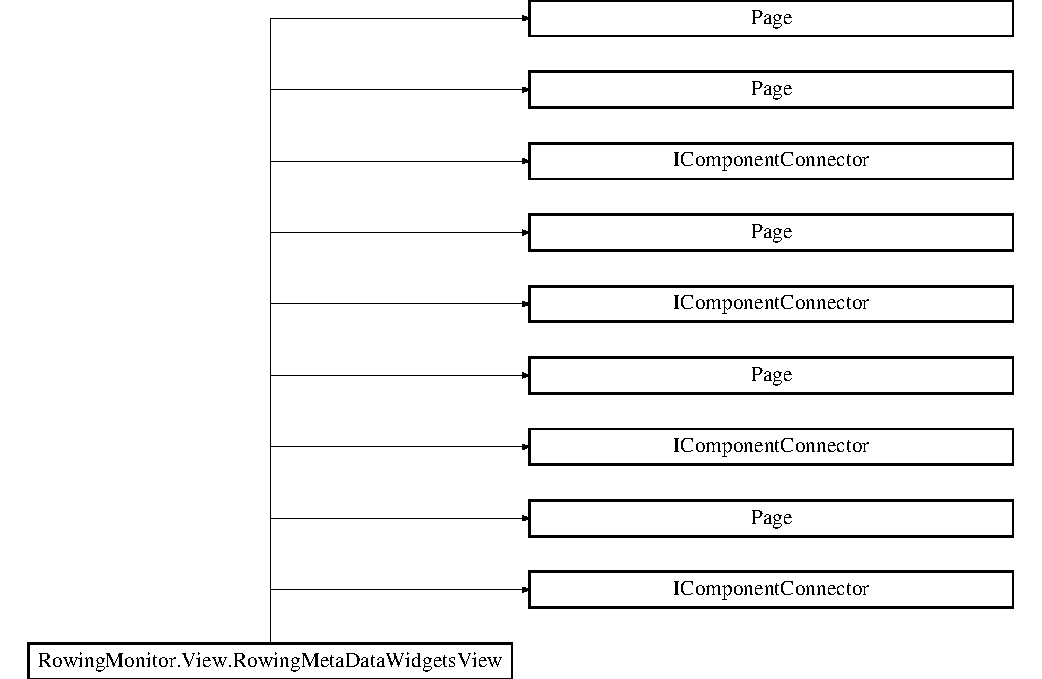
\includegraphics[height=9.120521cm]{class_rowing_monitor_1_1_view_1_1_rowing_meta_data_widgets_view}
\end{center}
\end{figure}
\subsection*{Public Member Functions}
\begin{DoxyCompactItemize}
\item 
void \hyperlink{class_rowing_monitor_1_1_view_1_1_rowing_meta_data_widgets_view_a156acf6faf9d7cd9925d2e164052d3d6}{Initialize\+Component} ()
\begin{DoxyCompactList}\small\item\em Initialize\+Component \end{DoxyCompactList}\item 
void \hyperlink{class_rowing_monitor_1_1_view_1_1_rowing_meta_data_widgets_view_a156acf6faf9d7cd9925d2e164052d3d6}{Initialize\+Component} ()
\begin{DoxyCompactList}\small\item\em Initialize\+Component \end{DoxyCompactList}\item 
void \hyperlink{class_rowing_monitor_1_1_view_1_1_rowing_meta_data_widgets_view_a156acf6faf9d7cd9925d2e164052d3d6}{Initialize\+Component} ()
\begin{DoxyCompactList}\small\item\em Initialize\+Component \end{DoxyCompactList}\item 
void \hyperlink{class_rowing_monitor_1_1_view_1_1_rowing_meta_data_widgets_view_a156acf6faf9d7cd9925d2e164052d3d6}{Initialize\+Component} ()
\begin{DoxyCompactList}\small\item\em Initialize\+Component \end{DoxyCompactList}\item 
\hyperlink{class_rowing_monitor_1_1_view_1_1_rowing_meta_data_widgets_view_a115912abc22b1d4f20694f03f5974502}{Rowing\+Meta\+Data\+Widgets\+View} ()
\end{DoxyCompactItemize}


\subsection{Detailed Description}
\hyperlink{class_rowing_monitor_1_1_view_1_1_rowing_meta_data_widgets_view}{Rowing\+Meta\+Data\+Widgets\+View} 

Interaktionslogik für Rowing\+Meta\+Data\+Widgets\+View.\+xaml 

\subsection{Constructor \& Destructor Documentation}
\mbox{\Hypertarget{class_rowing_monitor_1_1_view_1_1_rowing_meta_data_widgets_view_a115912abc22b1d4f20694f03f5974502}\label{class_rowing_monitor_1_1_view_1_1_rowing_meta_data_widgets_view_a115912abc22b1d4f20694f03f5974502}} 
\index{Rowing\+Monitor\+::\+View\+::\+Rowing\+Meta\+Data\+Widgets\+View@{Rowing\+Monitor\+::\+View\+::\+Rowing\+Meta\+Data\+Widgets\+View}!Rowing\+Meta\+Data\+Widgets\+View@{Rowing\+Meta\+Data\+Widgets\+View}}
\index{Rowing\+Meta\+Data\+Widgets\+View@{Rowing\+Meta\+Data\+Widgets\+View}!Rowing\+Monitor\+::\+View\+::\+Rowing\+Meta\+Data\+Widgets\+View@{Rowing\+Monitor\+::\+View\+::\+Rowing\+Meta\+Data\+Widgets\+View}}
\subsubsection{\texorpdfstring{Rowing\+Meta\+Data\+Widgets\+View()}{RowingMetaDataWidgetsView()}}
{\footnotesize\ttfamily Rowing\+Monitor.\+View.\+Rowing\+Meta\+Data\+Widgets\+View.\+Rowing\+Meta\+Data\+Widgets\+View (\begin{DoxyParamCaption}{ }\end{DoxyParamCaption})}



\subsection{Member Function Documentation}
\mbox{\Hypertarget{class_rowing_monitor_1_1_view_1_1_rowing_meta_data_widgets_view_a156acf6faf9d7cd9925d2e164052d3d6}\label{class_rowing_monitor_1_1_view_1_1_rowing_meta_data_widgets_view_a156acf6faf9d7cd9925d2e164052d3d6}} 
\index{Rowing\+Monitor\+::\+View\+::\+Rowing\+Meta\+Data\+Widgets\+View@{Rowing\+Monitor\+::\+View\+::\+Rowing\+Meta\+Data\+Widgets\+View}!Initialize\+Component@{Initialize\+Component}}
\index{Initialize\+Component@{Initialize\+Component}!Rowing\+Monitor\+::\+View\+::\+Rowing\+Meta\+Data\+Widgets\+View@{Rowing\+Monitor\+::\+View\+::\+Rowing\+Meta\+Data\+Widgets\+View}}
\subsubsection{\texorpdfstring{Initialize\+Component()}{InitializeComponent()}\hspace{0.1cm}{\footnotesize\ttfamily [1/4]}}
{\footnotesize\ttfamily void Rowing\+Monitor.\+View.\+Rowing\+Meta\+Data\+Widgets\+View.\+Initialize\+Component (\begin{DoxyParamCaption}{ }\end{DoxyParamCaption})}



Initialize\+Component 

\mbox{\Hypertarget{class_rowing_monitor_1_1_view_1_1_rowing_meta_data_widgets_view_a156acf6faf9d7cd9925d2e164052d3d6}\label{class_rowing_monitor_1_1_view_1_1_rowing_meta_data_widgets_view_a156acf6faf9d7cd9925d2e164052d3d6}} 
\index{Rowing\+Monitor\+::\+View\+::\+Rowing\+Meta\+Data\+Widgets\+View@{Rowing\+Monitor\+::\+View\+::\+Rowing\+Meta\+Data\+Widgets\+View}!Initialize\+Component@{Initialize\+Component}}
\index{Initialize\+Component@{Initialize\+Component}!Rowing\+Monitor\+::\+View\+::\+Rowing\+Meta\+Data\+Widgets\+View@{Rowing\+Monitor\+::\+View\+::\+Rowing\+Meta\+Data\+Widgets\+View}}
\subsubsection{\texorpdfstring{Initialize\+Component()}{InitializeComponent()}\hspace{0.1cm}{\footnotesize\ttfamily [2/4]}}
{\footnotesize\ttfamily void Rowing\+Monitor.\+View.\+Rowing\+Meta\+Data\+Widgets\+View.\+Initialize\+Component (\begin{DoxyParamCaption}{ }\end{DoxyParamCaption})}



Initialize\+Component 

\mbox{\Hypertarget{class_rowing_monitor_1_1_view_1_1_rowing_meta_data_widgets_view_a156acf6faf9d7cd9925d2e164052d3d6}\label{class_rowing_monitor_1_1_view_1_1_rowing_meta_data_widgets_view_a156acf6faf9d7cd9925d2e164052d3d6}} 
\index{Rowing\+Monitor\+::\+View\+::\+Rowing\+Meta\+Data\+Widgets\+View@{Rowing\+Monitor\+::\+View\+::\+Rowing\+Meta\+Data\+Widgets\+View}!Initialize\+Component@{Initialize\+Component}}
\index{Initialize\+Component@{Initialize\+Component}!Rowing\+Monitor\+::\+View\+::\+Rowing\+Meta\+Data\+Widgets\+View@{Rowing\+Monitor\+::\+View\+::\+Rowing\+Meta\+Data\+Widgets\+View}}
\subsubsection{\texorpdfstring{Initialize\+Component()}{InitializeComponent()}\hspace{0.1cm}{\footnotesize\ttfamily [3/4]}}
{\footnotesize\ttfamily void Rowing\+Monitor.\+View.\+Rowing\+Meta\+Data\+Widgets\+View.\+Initialize\+Component (\begin{DoxyParamCaption}{ }\end{DoxyParamCaption})}



Initialize\+Component 

\mbox{\Hypertarget{class_rowing_monitor_1_1_view_1_1_rowing_meta_data_widgets_view_a156acf6faf9d7cd9925d2e164052d3d6}\label{class_rowing_monitor_1_1_view_1_1_rowing_meta_data_widgets_view_a156acf6faf9d7cd9925d2e164052d3d6}} 
\index{Rowing\+Monitor\+::\+View\+::\+Rowing\+Meta\+Data\+Widgets\+View@{Rowing\+Monitor\+::\+View\+::\+Rowing\+Meta\+Data\+Widgets\+View}!Initialize\+Component@{Initialize\+Component}}
\index{Initialize\+Component@{Initialize\+Component}!Rowing\+Monitor\+::\+View\+::\+Rowing\+Meta\+Data\+Widgets\+View@{Rowing\+Monitor\+::\+View\+::\+Rowing\+Meta\+Data\+Widgets\+View}}
\subsubsection{\texorpdfstring{Initialize\+Component()}{InitializeComponent()}\hspace{0.1cm}{\footnotesize\ttfamily [4/4]}}
{\footnotesize\ttfamily void Rowing\+Monitor.\+View.\+Rowing\+Meta\+Data\+Widgets\+View.\+Initialize\+Component (\begin{DoxyParamCaption}{ }\end{DoxyParamCaption})}



Initialize\+Component 



The documentation for this class was generated from the following files\+:\begin{DoxyCompactItemize}
\item 
obj/\+Debug/\+View/\hyperlink{_debug_2_view_2_rowing_meta_data_widgets_view_8g_8cs}{Rowing\+Meta\+Data\+Widgets\+View.\+g.\+cs}\item 
obj/\+Debug/\+View/\hyperlink{_debug_2_view_2_rowing_meta_data_widgets_view_8g_8i_8cs}{Rowing\+Meta\+Data\+Widgets\+View.\+g.\+i.\+cs}\item 
View/\hyperlink{_rowing_meta_data_widgets_view_8xaml_8cs}{Rowing\+Meta\+Data\+Widgets\+View.\+xaml.\+cs}\end{DoxyCompactItemize}

\hypertarget{class_rowing_monitor_1_1_view_model_1_1_rowing_meta_data_widgets_view_model}{}\section{Rowing\+Monitor.\+View\+Model.\+Rowing\+Meta\+Data\+Widgets\+View\+Model Class Reference}
\label{class_rowing_monitor_1_1_view_model_1_1_rowing_meta_data_widgets_view_model}\index{Rowing\+Monitor.\+View\+Model.\+Rowing\+Meta\+Data\+Widgets\+View\+Model@{Rowing\+Monitor.\+View\+Model.\+Rowing\+Meta\+Data\+Widgets\+View\+Model}}
Inheritance diagram for Rowing\+Monitor.\+View\+Model.\+Rowing\+Meta\+Data\+Widgets\+View\+Model\+:\begin{figure}[H]
\begin{center}
\leavevmode
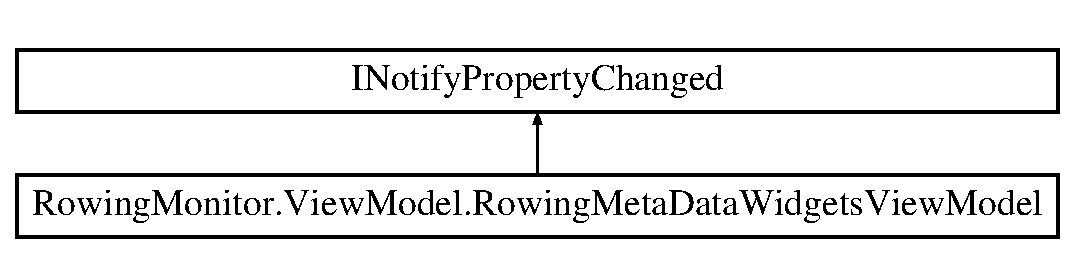
\includegraphics[height=2.000000cm]{class_rowing_monitor_1_1_view_model_1_1_rowing_meta_data_widgets_view_model}
\end{center}
\end{figure}
\subsection*{Public Member Functions}
\begin{DoxyCompactItemize}
\item 
void \hyperlink{class_rowing_monitor_1_1_view_model_1_1_rowing_meta_data_widgets_view_model_a272d9f725b957aadf11817c893020636}{Render} (double catch\+Factor, double rowing\+Style\+Factor)
\end{DoxyCompactItemize}
\subsection*{Properties}
\begin{DoxyCompactItemize}
\item 
Thickness \hyperlink{class_rowing_monitor_1_1_view_model_1_1_rowing_meta_data_widgets_view_model_a2dedfb7b57cfcd67b61e777b14891a1e}{Catch\+Factor\+Margin}\hspace{0.3cm}{\ttfamily  \mbox{[}get, set\mbox{]}}
\item 
Thickness \hyperlink{class_rowing_monitor_1_1_view_model_1_1_rowing_meta_data_widgets_view_model_acfee03e813686ca119576f0abbf83c87}{Rowing\+Style\+Factor\+Margin}\hspace{0.3cm}{\ttfamily  \mbox{[}get, set\mbox{]}}
\item 
string \hyperlink{class_rowing_monitor_1_1_view_model_1_1_rowing_meta_data_widgets_view_model_a209ec36ede2c8cdbfcb12630d28218b2}{Catch\+Factor}\hspace{0.3cm}{\ttfamily  \mbox{[}get, set\mbox{]}}
\item 
string \hyperlink{class_rowing_monitor_1_1_view_model_1_1_rowing_meta_data_widgets_view_model_a9d85f12031925615071fcd2a7ac53d26}{Rowing\+Style\+Factor}\hspace{0.3cm}{\ttfamily  \mbox{[}get, set\mbox{]}}
\item 
Brush \hyperlink{class_rowing_monitor_1_1_view_model_1_1_rowing_meta_data_widgets_view_model_aa93ca40fd565fffd75085d27262d242b}{Catch\+Factor\+Color}\hspace{0.3cm}{\ttfamily  \mbox{[}get, set\mbox{]}}
\item 
Brush \hyperlink{class_rowing_monitor_1_1_view_model_1_1_rowing_meta_data_widgets_view_model_abab0580c7f52967dc957aed741b52673}{Rowing\+Style\+Factor\+Color}\hspace{0.3cm}{\ttfamily  \mbox{[}get, set\mbox{]}}
\end{DoxyCompactItemize}
\subsection*{Events}
\begin{DoxyCompactItemize}
\item 
Property\+Changed\+Event\+Handler \hyperlink{class_rowing_monitor_1_1_view_model_1_1_rowing_meta_data_widgets_view_model_a4661a90884262be4e23ae44e73db22df}{Property\+Changed}
\end{DoxyCompactItemize}


\subsection{Member Function Documentation}
\mbox{\Hypertarget{class_rowing_monitor_1_1_view_model_1_1_rowing_meta_data_widgets_view_model_a272d9f725b957aadf11817c893020636}\label{class_rowing_monitor_1_1_view_model_1_1_rowing_meta_data_widgets_view_model_a272d9f725b957aadf11817c893020636}} 
\index{Rowing\+Monitor\+::\+View\+Model\+::\+Rowing\+Meta\+Data\+Widgets\+View\+Model@{Rowing\+Monitor\+::\+View\+Model\+::\+Rowing\+Meta\+Data\+Widgets\+View\+Model}!Render@{Render}}
\index{Render@{Render}!Rowing\+Monitor\+::\+View\+Model\+::\+Rowing\+Meta\+Data\+Widgets\+View\+Model@{Rowing\+Monitor\+::\+View\+Model\+::\+Rowing\+Meta\+Data\+Widgets\+View\+Model}}
\subsubsection{\texorpdfstring{Render()}{Render()}}
{\footnotesize\ttfamily void Rowing\+Monitor.\+View\+Model.\+Rowing\+Meta\+Data\+Widgets\+View\+Model.\+Render (\begin{DoxyParamCaption}\item[{double}]{catch\+Factor,  }\item[{double}]{rowing\+Style\+Factor }\end{DoxyParamCaption})}



\subsection{Property Documentation}
\mbox{\Hypertarget{class_rowing_monitor_1_1_view_model_1_1_rowing_meta_data_widgets_view_model_a209ec36ede2c8cdbfcb12630d28218b2}\label{class_rowing_monitor_1_1_view_model_1_1_rowing_meta_data_widgets_view_model_a209ec36ede2c8cdbfcb12630d28218b2}} 
\index{Rowing\+Monitor\+::\+View\+Model\+::\+Rowing\+Meta\+Data\+Widgets\+View\+Model@{Rowing\+Monitor\+::\+View\+Model\+::\+Rowing\+Meta\+Data\+Widgets\+View\+Model}!Catch\+Factor@{Catch\+Factor}}
\index{Catch\+Factor@{Catch\+Factor}!Rowing\+Monitor\+::\+View\+Model\+::\+Rowing\+Meta\+Data\+Widgets\+View\+Model@{Rowing\+Monitor\+::\+View\+Model\+::\+Rowing\+Meta\+Data\+Widgets\+View\+Model}}
\subsubsection{\texorpdfstring{Catch\+Factor}{CatchFactor}}
{\footnotesize\ttfamily string Rowing\+Monitor.\+View\+Model.\+Rowing\+Meta\+Data\+Widgets\+View\+Model.\+Catch\+Factor\hspace{0.3cm}{\ttfamily [get]}, {\ttfamily [set]}}

\mbox{\Hypertarget{class_rowing_monitor_1_1_view_model_1_1_rowing_meta_data_widgets_view_model_aa93ca40fd565fffd75085d27262d242b}\label{class_rowing_monitor_1_1_view_model_1_1_rowing_meta_data_widgets_view_model_aa93ca40fd565fffd75085d27262d242b}} 
\index{Rowing\+Monitor\+::\+View\+Model\+::\+Rowing\+Meta\+Data\+Widgets\+View\+Model@{Rowing\+Monitor\+::\+View\+Model\+::\+Rowing\+Meta\+Data\+Widgets\+View\+Model}!Catch\+Factor\+Color@{Catch\+Factor\+Color}}
\index{Catch\+Factor\+Color@{Catch\+Factor\+Color}!Rowing\+Monitor\+::\+View\+Model\+::\+Rowing\+Meta\+Data\+Widgets\+View\+Model@{Rowing\+Monitor\+::\+View\+Model\+::\+Rowing\+Meta\+Data\+Widgets\+View\+Model}}
\subsubsection{\texorpdfstring{Catch\+Factor\+Color}{CatchFactorColor}}
{\footnotesize\ttfamily Brush Rowing\+Monitor.\+View\+Model.\+Rowing\+Meta\+Data\+Widgets\+View\+Model.\+Catch\+Factor\+Color\hspace{0.3cm}{\ttfamily [get]}, {\ttfamily [set]}}

\mbox{\Hypertarget{class_rowing_monitor_1_1_view_model_1_1_rowing_meta_data_widgets_view_model_a2dedfb7b57cfcd67b61e777b14891a1e}\label{class_rowing_monitor_1_1_view_model_1_1_rowing_meta_data_widgets_view_model_a2dedfb7b57cfcd67b61e777b14891a1e}} 
\index{Rowing\+Monitor\+::\+View\+Model\+::\+Rowing\+Meta\+Data\+Widgets\+View\+Model@{Rowing\+Monitor\+::\+View\+Model\+::\+Rowing\+Meta\+Data\+Widgets\+View\+Model}!Catch\+Factor\+Margin@{Catch\+Factor\+Margin}}
\index{Catch\+Factor\+Margin@{Catch\+Factor\+Margin}!Rowing\+Monitor\+::\+View\+Model\+::\+Rowing\+Meta\+Data\+Widgets\+View\+Model@{Rowing\+Monitor\+::\+View\+Model\+::\+Rowing\+Meta\+Data\+Widgets\+View\+Model}}
\subsubsection{\texorpdfstring{Catch\+Factor\+Margin}{CatchFactorMargin}}
{\footnotesize\ttfamily Thickness Rowing\+Monitor.\+View\+Model.\+Rowing\+Meta\+Data\+Widgets\+View\+Model.\+Catch\+Factor\+Margin\hspace{0.3cm}{\ttfamily [get]}, {\ttfamily [set]}}

\mbox{\Hypertarget{class_rowing_monitor_1_1_view_model_1_1_rowing_meta_data_widgets_view_model_a9d85f12031925615071fcd2a7ac53d26}\label{class_rowing_monitor_1_1_view_model_1_1_rowing_meta_data_widgets_view_model_a9d85f12031925615071fcd2a7ac53d26}} 
\index{Rowing\+Monitor\+::\+View\+Model\+::\+Rowing\+Meta\+Data\+Widgets\+View\+Model@{Rowing\+Monitor\+::\+View\+Model\+::\+Rowing\+Meta\+Data\+Widgets\+View\+Model}!Rowing\+Style\+Factor@{Rowing\+Style\+Factor}}
\index{Rowing\+Style\+Factor@{Rowing\+Style\+Factor}!Rowing\+Monitor\+::\+View\+Model\+::\+Rowing\+Meta\+Data\+Widgets\+View\+Model@{Rowing\+Monitor\+::\+View\+Model\+::\+Rowing\+Meta\+Data\+Widgets\+View\+Model}}
\subsubsection{\texorpdfstring{Rowing\+Style\+Factor}{RowingStyleFactor}}
{\footnotesize\ttfamily string Rowing\+Monitor.\+View\+Model.\+Rowing\+Meta\+Data\+Widgets\+View\+Model.\+Rowing\+Style\+Factor\hspace{0.3cm}{\ttfamily [get]}, {\ttfamily [set]}}

\mbox{\Hypertarget{class_rowing_monitor_1_1_view_model_1_1_rowing_meta_data_widgets_view_model_abab0580c7f52967dc957aed741b52673}\label{class_rowing_monitor_1_1_view_model_1_1_rowing_meta_data_widgets_view_model_abab0580c7f52967dc957aed741b52673}} 
\index{Rowing\+Monitor\+::\+View\+Model\+::\+Rowing\+Meta\+Data\+Widgets\+View\+Model@{Rowing\+Monitor\+::\+View\+Model\+::\+Rowing\+Meta\+Data\+Widgets\+View\+Model}!Rowing\+Style\+Factor\+Color@{Rowing\+Style\+Factor\+Color}}
\index{Rowing\+Style\+Factor\+Color@{Rowing\+Style\+Factor\+Color}!Rowing\+Monitor\+::\+View\+Model\+::\+Rowing\+Meta\+Data\+Widgets\+View\+Model@{Rowing\+Monitor\+::\+View\+Model\+::\+Rowing\+Meta\+Data\+Widgets\+View\+Model}}
\subsubsection{\texorpdfstring{Rowing\+Style\+Factor\+Color}{RowingStyleFactorColor}}
{\footnotesize\ttfamily Brush Rowing\+Monitor.\+View\+Model.\+Rowing\+Meta\+Data\+Widgets\+View\+Model.\+Rowing\+Style\+Factor\+Color\hspace{0.3cm}{\ttfamily [get]}, {\ttfamily [set]}}

\mbox{\Hypertarget{class_rowing_monitor_1_1_view_model_1_1_rowing_meta_data_widgets_view_model_acfee03e813686ca119576f0abbf83c87}\label{class_rowing_monitor_1_1_view_model_1_1_rowing_meta_data_widgets_view_model_acfee03e813686ca119576f0abbf83c87}} 
\index{Rowing\+Monitor\+::\+View\+Model\+::\+Rowing\+Meta\+Data\+Widgets\+View\+Model@{Rowing\+Monitor\+::\+View\+Model\+::\+Rowing\+Meta\+Data\+Widgets\+View\+Model}!Rowing\+Style\+Factor\+Margin@{Rowing\+Style\+Factor\+Margin}}
\index{Rowing\+Style\+Factor\+Margin@{Rowing\+Style\+Factor\+Margin}!Rowing\+Monitor\+::\+View\+Model\+::\+Rowing\+Meta\+Data\+Widgets\+View\+Model@{Rowing\+Monitor\+::\+View\+Model\+::\+Rowing\+Meta\+Data\+Widgets\+View\+Model}}
\subsubsection{\texorpdfstring{Rowing\+Style\+Factor\+Margin}{RowingStyleFactorMargin}}
{\footnotesize\ttfamily Thickness Rowing\+Monitor.\+View\+Model.\+Rowing\+Meta\+Data\+Widgets\+View\+Model.\+Rowing\+Style\+Factor\+Margin\hspace{0.3cm}{\ttfamily [get]}, {\ttfamily [set]}}



\subsection{Event Documentation}
\mbox{\Hypertarget{class_rowing_monitor_1_1_view_model_1_1_rowing_meta_data_widgets_view_model_a4661a90884262be4e23ae44e73db22df}\label{class_rowing_monitor_1_1_view_model_1_1_rowing_meta_data_widgets_view_model_a4661a90884262be4e23ae44e73db22df}} 
\index{Rowing\+Monitor\+::\+View\+Model\+::\+Rowing\+Meta\+Data\+Widgets\+View\+Model@{Rowing\+Monitor\+::\+View\+Model\+::\+Rowing\+Meta\+Data\+Widgets\+View\+Model}!Property\+Changed@{Property\+Changed}}
\index{Property\+Changed@{Property\+Changed}!Rowing\+Monitor\+::\+View\+Model\+::\+Rowing\+Meta\+Data\+Widgets\+View\+Model@{Rowing\+Monitor\+::\+View\+Model\+::\+Rowing\+Meta\+Data\+Widgets\+View\+Model}}
\subsubsection{\texorpdfstring{Property\+Changed}{PropertyChanged}}
{\footnotesize\ttfamily Property\+Changed\+Event\+Handler Rowing\+Monitor.\+View\+Model.\+Rowing\+Meta\+Data\+Widgets\+View\+Model.\+Property\+Changed}



The documentation for this class was generated from the following file\+:\begin{DoxyCompactItemize}
\item 
View\+Model/\hyperlink{_rowing_meta_data_widgets_view_model_8cs}{Rowing\+Meta\+Data\+Widgets\+View\+Model.\+cs}\end{DoxyCompactItemize}

\hypertarget{class_rowing_monitor_1_1_rowing_monitor_window}{}\section{Rowing\+Monitor.\+Rowing\+Monitor\+Window Class Reference}
\label{class_rowing_monitor_1_1_rowing_monitor_window}\index{Rowing\+Monitor.\+Rowing\+Monitor\+Window@{Rowing\+Monitor.\+Rowing\+Monitor\+Window}}


\hyperlink{class_rowing_monitor_1_1_rowing_monitor_window}{Rowing\+Monitor\+Window}  


Inheritance diagram for Rowing\+Monitor.\+Rowing\+Monitor\+Window\+:\begin{figure}[H]
\begin{center}
\leavevmode
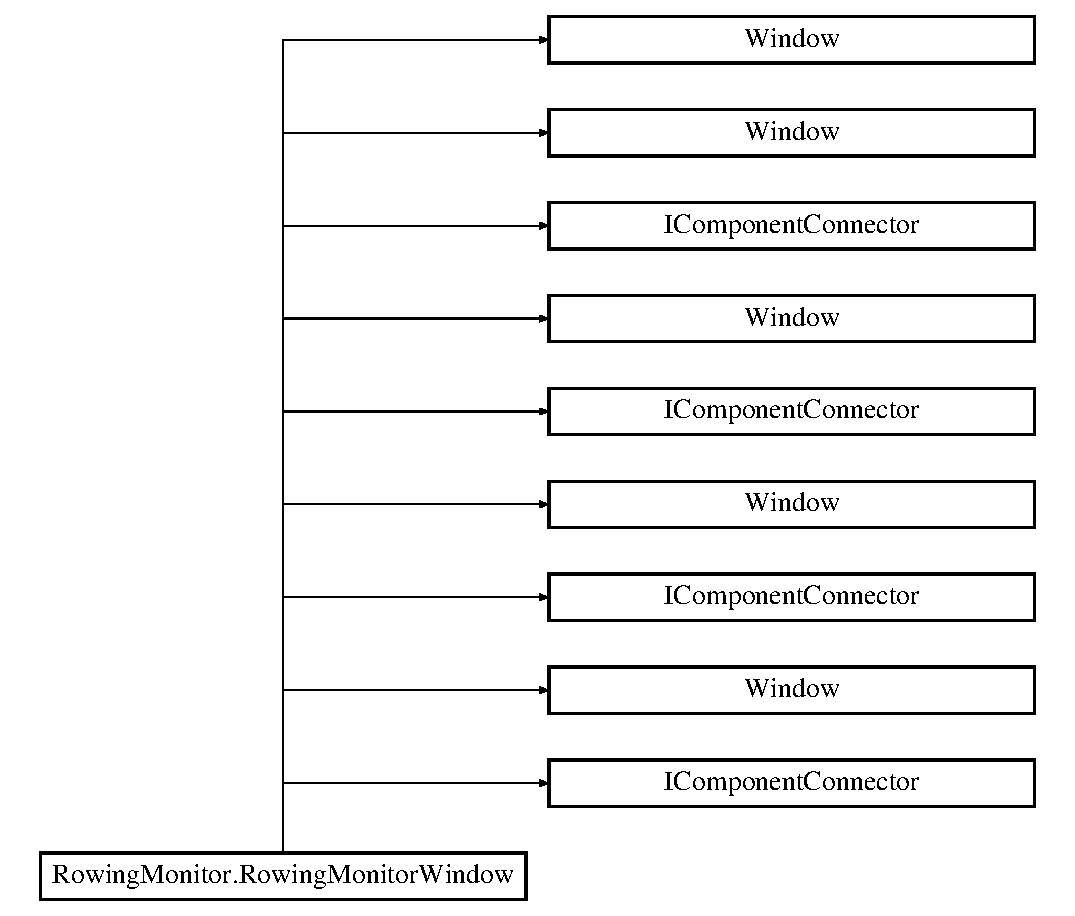
\includegraphics[height=10.000000cm]{class_rowing_monitor_1_1_rowing_monitor_window}
\end{center}
\end{figure}
\subsection*{Public Member Functions}
\begin{DoxyCompactItemize}
\item 
void \hyperlink{class_rowing_monitor_1_1_rowing_monitor_window_ace5d64ad5ace3448f5390d3bb57ddc2e}{Initialize\+Component} ()
\begin{DoxyCompactList}\small\item\em Initialize\+Component \end{DoxyCompactList}\item 
void \hyperlink{class_rowing_monitor_1_1_rowing_monitor_window_ace5d64ad5ace3448f5390d3bb57ddc2e}{Initialize\+Component} ()
\begin{DoxyCompactList}\small\item\em Initialize\+Component \end{DoxyCompactList}\item 
void \hyperlink{class_rowing_monitor_1_1_rowing_monitor_window_ace5d64ad5ace3448f5390d3bb57ddc2e}{Initialize\+Component} ()
\begin{DoxyCompactList}\small\item\em Initialize\+Component \end{DoxyCompactList}\item 
void \hyperlink{class_rowing_monitor_1_1_rowing_monitor_window_ace5d64ad5ace3448f5390d3bb57ddc2e}{Initialize\+Component} ()
\begin{DoxyCompactList}\small\item\em Initialize\+Component \end{DoxyCompactList}\item 
\hyperlink{class_rowing_monitor_1_1_rowing_monitor_window_aa2e686844acc551384743df9d9eebf42}{Rowing\+Monitor\+Window} ()
\end{DoxyCompactItemize}


\subsection{Detailed Description}
\hyperlink{class_rowing_monitor_1_1_rowing_monitor_window}{Rowing\+Monitor\+Window} 

Interaktionslogik für Rowing\+Monitor\+Window.\+xaml 

\subsection{Constructor \& Destructor Documentation}
\mbox{\Hypertarget{class_rowing_monitor_1_1_rowing_monitor_window_aa2e686844acc551384743df9d9eebf42}\label{class_rowing_monitor_1_1_rowing_monitor_window_aa2e686844acc551384743df9d9eebf42}} 
\index{Rowing\+Monitor\+::\+Rowing\+Monitor\+Window@{Rowing\+Monitor\+::\+Rowing\+Monitor\+Window}!Rowing\+Monitor\+Window@{Rowing\+Monitor\+Window}}
\index{Rowing\+Monitor\+Window@{Rowing\+Monitor\+Window}!Rowing\+Monitor\+::\+Rowing\+Monitor\+Window@{Rowing\+Monitor\+::\+Rowing\+Monitor\+Window}}
\subsubsection{\texorpdfstring{Rowing\+Monitor\+Window()}{RowingMonitorWindow()}}
{\footnotesize\ttfamily Rowing\+Monitor.\+Rowing\+Monitor\+Window.\+Rowing\+Monitor\+Window (\begin{DoxyParamCaption}{ }\end{DoxyParamCaption})}



\subsection{Member Function Documentation}
\mbox{\Hypertarget{class_rowing_monitor_1_1_rowing_monitor_window_ace5d64ad5ace3448f5390d3bb57ddc2e}\label{class_rowing_monitor_1_1_rowing_monitor_window_ace5d64ad5ace3448f5390d3bb57ddc2e}} 
\index{Rowing\+Monitor\+::\+Rowing\+Monitor\+Window@{Rowing\+Monitor\+::\+Rowing\+Monitor\+Window}!Initialize\+Component@{Initialize\+Component}}
\index{Initialize\+Component@{Initialize\+Component}!Rowing\+Monitor\+::\+Rowing\+Monitor\+Window@{Rowing\+Monitor\+::\+Rowing\+Monitor\+Window}}
\subsubsection{\texorpdfstring{Initialize\+Component()}{InitializeComponent()}\hspace{0.1cm}{\footnotesize\ttfamily [1/4]}}
{\footnotesize\ttfamily void Rowing\+Monitor.\+Rowing\+Monitor\+Window.\+Initialize\+Component (\begin{DoxyParamCaption}{ }\end{DoxyParamCaption})}



Initialize\+Component 

\mbox{\Hypertarget{class_rowing_monitor_1_1_rowing_monitor_window_ace5d64ad5ace3448f5390d3bb57ddc2e}\label{class_rowing_monitor_1_1_rowing_monitor_window_ace5d64ad5ace3448f5390d3bb57ddc2e}} 
\index{Rowing\+Monitor\+::\+Rowing\+Monitor\+Window@{Rowing\+Monitor\+::\+Rowing\+Monitor\+Window}!Initialize\+Component@{Initialize\+Component}}
\index{Initialize\+Component@{Initialize\+Component}!Rowing\+Monitor\+::\+Rowing\+Monitor\+Window@{Rowing\+Monitor\+::\+Rowing\+Monitor\+Window}}
\subsubsection{\texorpdfstring{Initialize\+Component()}{InitializeComponent()}\hspace{0.1cm}{\footnotesize\ttfamily [2/4]}}
{\footnotesize\ttfamily void Rowing\+Monitor.\+Rowing\+Monitor\+Window.\+Initialize\+Component (\begin{DoxyParamCaption}{ }\end{DoxyParamCaption})}



Initialize\+Component 

\mbox{\Hypertarget{class_rowing_monitor_1_1_rowing_monitor_window_ace5d64ad5ace3448f5390d3bb57ddc2e}\label{class_rowing_monitor_1_1_rowing_monitor_window_ace5d64ad5ace3448f5390d3bb57ddc2e}} 
\index{Rowing\+Monitor\+::\+Rowing\+Monitor\+Window@{Rowing\+Monitor\+::\+Rowing\+Monitor\+Window}!Initialize\+Component@{Initialize\+Component}}
\index{Initialize\+Component@{Initialize\+Component}!Rowing\+Monitor\+::\+Rowing\+Monitor\+Window@{Rowing\+Monitor\+::\+Rowing\+Monitor\+Window}}
\subsubsection{\texorpdfstring{Initialize\+Component()}{InitializeComponent()}\hspace{0.1cm}{\footnotesize\ttfamily [3/4]}}
{\footnotesize\ttfamily void Rowing\+Monitor.\+Rowing\+Monitor\+Window.\+Initialize\+Component (\begin{DoxyParamCaption}{ }\end{DoxyParamCaption})}



Initialize\+Component 

\mbox{\Hypertarget{class_rowing_monitor_1_1_rowing_monitor_window_ace5d64ad5ace3448f5390d3bb57ddc2e}\label{class_rowing_monitor_1_1_rowing_monitor_window_ace5d64ad5ace3448f5390d3bb57ddc2e}} 
\index{Rowing\+Monitor\+::\+Rowing\+Monitor\+Window@{Rowing\+Monitor\+::\+Rowing\+Monitor\+Window}!Initialize\+Component@{Initialize\+Component}}
\index{Initialize\+Component@{Initialize\+Component}!Rowing\+Monitor\+::\+Rowing\+Monitor\+Window@{Rowing\+Monitor\+::\+Rowing\+Monitor\+Window}}
\subsubsection{\texorpdfstring{Initialize\+Component()}{InitializeComponent()}\hspace{0.1cm}{\footnotesize\ttfamily [4/4]}}
{\footnotesize\ttfamily void Rowing\+Monitor.\+Rowing\+Monitor\+Window.\+Initialize\+Component (\begin{DoxyParamCaption}{ }\end{DoxyParamCaption})}



Initialize\+Component 



The documentation for this class was generated from the following files\+:\begin{DoxyCompactItemize}
\item 
obj/\+Debug/\hyperlink{_debug_2_rowing_monitor_window_8g_8cs}{Rowing\+Monitor\+Window.\+g.\+cs}\item 
obj/\+Debug/\hyperlink{_debug_2_rowing_monitor_window_8g_8i_8cs}{Rowing\+Monitor\+Window.\+g.\+i.\+cs}\item 
\hyperlink{_rowing_monitor_window_8xaml_8cs}{Rowing\+Monitor\+Window.\+xaml.\+cs}\end{DoxyCompactItemize}

\hypertarget{class_rowing_monitor_1_1_model_1_1_pipeline_1_1_rowing_sonification}{}\section{Rowing\+Monitor.\+Model.\+Pipeline.\+Rowing\+Sonification Class Reference}
\label{class_rowing_monitor_1_1_model_1_1_pipeline_1_1_rowing_sonification}\index{Rowing\+Monitor.\+Model.\+Pipeline.\+Rowing\+Sonification@{Rowing\+Monitor.\+Model.\+Pipeline.\+Rowing\+Sonification}}
\subsection*{Public Member Functions}
\begin{DoxyCompactItemize}
\item 
\hyperlink{class_rowing_monitor_1_1_model_1_1_pipeline_1_1_rowing_sonification_aa3189ffe2f7c36a9cc5afaad8c7d896d}{Rowing\+Sonification} ()
\end{DoxyCompactItemize}
\subsection*{Properties}
\begin{DoxyCompactItemize}
\item 
bool \hyperlink{class_rowing_monitor_1_1_model_1_1_pipeline_1_1_rowing_sonification_af076633c8ac6e8f30336b0ca0bb891e0}{Mute}\hspace{0.3cm}{\ttfamily  \mbox{[}get, set\mbox{]}}
\item 
Action\+Block$<$ \hyperlink{struct_rowing_monitor_1_1_model_1_1_pipeline_1_1_kleshnev_data}{Kleshnev\+Data} $>$ \hyperlink{class_rowing_monitor_1_1_model_1_1_pipeline_1_1_rowing_sonification_aa36c7f6801b612cb4363e2c0338e6e70}{Input}\hspace{0.3cm}{\ttfamily  \mbox{[}get, set\mbox{]}}
\item 
Action\+Block$<$ List$<$ \hyperlink{struct_rowing_monitor_1_1_model_1_1_util_1_1_segment_hit}{Segment\+Hit} $>$ $>$ \hyperlink{class_rowing_monitor_1_1_model_1_1_pipeline_1_1_rowing_sonification_a52fbdd66e6e0d5a8a936df0a193ab59a}{Input\+Segment\+Hits}\hspace{0.3cm}{\ttfamily  \mbox{[}get, set\mbox{]}}
\end{DoxyCompactItemize}


\subsection{Constructor \& Destructor Documentation}
\mbox{\Hypertarget{class_rowing_monitor_1_1_model_1_1_pipeline_1_1_rowing_sonification_aa3189ffe2f7c36a9cc5afaad8c7d896d}\label{class_rowing_monitor_1_1_model_1_1_pipeline_1_1_rowing_sonification_aa3189ffe2f7c36a9cc5afaad8c7d896d}} 
\index{Rowing\+Monitor\+::\+Model\+::\+Pipeline\+::\+Rowing\+Sonification@{Rowing\+Monitor\+::\+Model\+::\+Pipeline\+::\+Rowing\+Sonification}!Rowing\+Sonification@{Rowing\+Sonification}}
\index{Rowing\+Sonification@{Rowing\+Sonification}!Rowing\+Monitor\+::\+Model\+::\+Pipeline\+::\+Rowing\+Sonification@{Rowing\+Monitor\+::\+Model\+::\+Pipeline\+::\+Rowing\+Sonification}}
\subsubsection{\texorpdfstring{Rowing\+Sonification()}{RowingSonification()}}
{\footnotesize\ttfamily Rowing\+Monitor.\+Model.\+Pipeline.\+Rowing\+Sonification.\+Rowing\+Sonification (\begin{DoxyParamCaption}{ }\end{DoxyParamCaption})}



\subsection{Property Documentation}
\mbox{\Hypertarget{class_rowing_monitor_1_1_model_1_1_pipeline_1_1_rowing_sonification_aa36c7f6801b612cb4363e2c0338e6e70}\label{class_rowing_monitor_1_1_model_1_1_pipeline_1_1_rowing_sonification_aa36c7f6801b612cb4363e2c0338e6e70}} 
\index{Rowing\+Monitor\+::\+Model\+::\+Pipeline\+::\+Rowing\+Sonification@{Rowing\+Monitor\+::\+Model\+::\+Pipeline\+::\+Rowing\+Sonification}!Input@{Input}}
\index{Input@{Input}!Rowing\+Monitor\+::\+Model\+::\+Pipeline\+::\+Rowing\+Sonification@{Rowing\+Monitor\+::\+Model\+::\+Pipeline\+::\+Rowing\+Sonification}}
\subsubsection{\texorpdfstring{Input}{Input}}
{\footnotesize\ttfamily Action\+Block$<$\hyperlink{struct_rowing_monitor_1_1_model_1_1_pipeline_1_1_kleshnev_data}{Kleshnev\+Data}$>$ Rowing\+Monitor.\+Model.\+Pipeline.\+Rowing\+Sonification.\+Input\hspace{0.3cm}{\ttfamily [get]}, {\ttfamily [set]}}

\mbox{\Hypertarget{class_rowing_monitor_1_1_model_1_1_pipeline_1_1_rowing_sonification_a52fbdd66e6e0d5a8a936df0a193ab59a}\label{class_rowing_monitor_1_1_model_1_1_pipeline_1_1_rowing_sonification_a52fbdd66e6e0d5a8a936df0a193ab59a}} 
\index{Rowing\+Monitor\+::\+Model\+::\+Pipeline\+::\+Rowing\+Sonification@{Rowing\+Monitor\+::\+Model\+::\+Pipeline\+::\+Rowing\+Sonification}!Input\+Segment\+Hits@{Input\+Segment\+Hits}}
\index{Input\+Segment\+Hits@{Input\+Segment\+Hits}!Rowing\+Monitor\+::\+Model\+::\+Pipeline\+::\+Rowing\+Sonification@{Rowing\+Monitor\+::\+Model\+::\+Pipeline\+::\+Rowing\+Sonification}}
\subsubsection{\texorpdfstring{Input\+Segment\+Hits}{InputSegmentHits}}
{\footnotesize\ttfamily Action\+Block$<$List$<$\hyperlink{struct_rowing_monitor_1_1_model_1_1_util_1_1_segment_hit}{Segment\+Hit}$>$ $>$ Rowing\+Monitor.\+Model.\+Pipeline.\+Rowing\+Sonification.\+Input\+Segment\+Hits\hspace{0.3cm}{\ttfamily [get]}, {\ttfamily [set]}}

\mbox{\Hypertarget{class_rowing_monitor_1_1_model_1_1_pipeline_1_1_rowing_sonification_af076633c8ac6e8f30336b0ca0bb891e0}\label{class_rowing_monitor_1_1_model_1_1_pipeline_1_1_rowing_sonification_af076633c8ac6e8f30336b0ca0bb891e0}} 
\index{Rowing\+Monitor\+::\+Model\+::\+Pipeline\+::\+Rowing\+Sonification@{Rowing\+Monitor\+::\+Model\+::\+Pipeline\+::\+Rowing\+Sonification}!Mute@{Mute}}
\index{Mute@{Mute}!Rowing\+Monitor\+::\+Model\+::\+Pipeline\+::\+Rowing\+Sonification@{Rowing\+Monitor\+::\+Model\+::\+Pipeline\+::\+Rowing\+Sonification}}
\subsubsection{\texorpdfstring{Mute}{Mute}}
{\footnotesize\ttfamily bool Rowing\+Monitor.\+Model.\+Pipeline.\+Rowing\+Sonification.\+Mute\hspace{0.3cm}{\ttfamily [get]}, {\ttfamily [set]}}



The documentation for this class was generated from the following file\+:\begin{DoxyCompactItemize}
\item 
Model/\+Pipeline/\hyperlink{_rowing_sonification_8cs}{Rowing\+Sonification.\+cs}\end{DoxyCompactItemize}

\hypertarget{class_rowing_monitor_1_1_model_1_1_segment_detected_event_args}{}\section{Rowing\+Monitor.\+Model.\+Segment\+Detected\+Event\+Args Class Reference}
\label{class_rowing_monitor_1_1_model_1_1_segment_detected_event_args}\index{Rowing\+Monitor.\+Model.\+Segment\+Detected\+Event\+Args@{Rowing\+Monitor.\+Model.\+Segment\+Detected\+Event\+Args}}


Represents the arguments for a detected segment event.  


Inheritance diagram for Rowing\+Monitor.\+Model.\+Segment\+Detected\+Event\+Args\+:\begin{figure}[H]
\begin{center}
\leavevmode
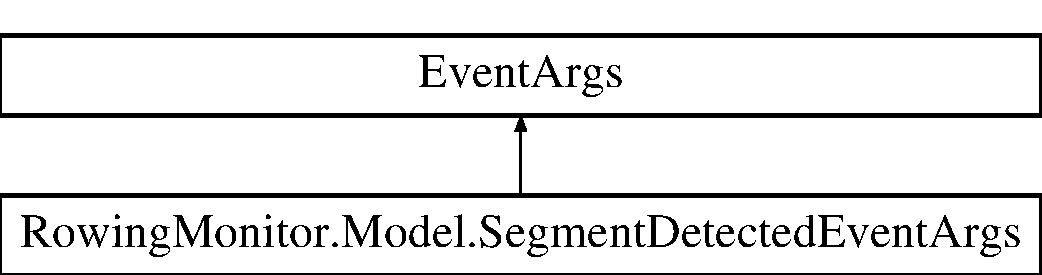
\includegraphics[height=2.000000cm]{class_rowing_monitor_1_1_model_1_1_segment_detected_event_args}
\end{center}
\end{figure}
\subsection*{Public Member Functions}
\begin{DoxyCompactItemize}
\item 
\hyperlink{class_rowing_monitor_1_1_model_1_1_segment_detected_event_args_ae0faa5e59bb3acdbfed39c7f1a44bd4d}{Segment\+Detected\+Event\+Args} (List$<$ \hyperlink{struct_rowing_monitor_1_1_model_1_1_util_1_1_segment_hit}{Segment\+Hit} $>$ hits)
\end{DoxyCompactItemize}
\subsection*{Properties}
\begin{DoxyCompactItemize}
\item 
List$<$ \hyperlink{struct_rowing_monitor_1_1_model_1_1_util_1_1_segment_hit}{Segment\+Hit} $>$ \hyperlink{class_rowing_monitor_1_1_model_1_1_segment_detected_event_args_aa2a7633ef1c061df79fb2932261e0359}{Hits}\hspace{0.3cm}{\ttfamily  \mbox{[}get\mbox{]}}
\end{DoxyCompactItemize}


\subsection{Detailed Description}
Represents the arguments for a detected segment event. 



\subsection{Constructor \& Destructor Documentation}
\mbox{\Hypertarget{class_rowing_monitor_1_1_model_1_1_segment_detected_event_args_ae0faa5e59bb3acdbfed39c7f1a44bd4d}\label{class_rowing_monitor_1_1_model_1_1_segment_detected_event_args_ae0faa5e59bb3acdbfed39c7f1a44bd4d}} 
\index{Rowing\+Monitor\+::\+Model\+::\+Segment\+Detected\+Event\+Args@{Rowing\+Monitor\+::\+Model\+::\+Segment\+Detected\+Event\+Args}!Segment\+Detected\+Event\+Args@{Segment\+Detected\+Event\+Args}}
\index{Segment\+Detected\+Event\+Args@{Segment\+Detected\+Event\+Args}!Rowing\+Monitor\+::\+Model\+::\+Segment\+Detected\+Event\+Args@{Rowing\+Monitor\+::\+Model\+::\+Segment\+Detected\+Event\+Args}}
\subsubsection{\texorpdfstring{Segment\+Detected\+Event\+Args()}{SegmentDetectedEventArgs()}}
{\footnotesize\ttfamily Rowing\+Monitor.\+Model.\+Segment\+Detected\+Event\+Args.\+Segment\+Detected\+Event\+Args (\begin{DoxyParamCaption}\item[{List$<$ \hyperlink{struct_rowing_monitor_1_1_model_1_1_util_1_1_segment_hit}{Segment\+Hit} $>$}]{hits }\end{DoxyParamCaption})}



\subsection{Property Documentation}
\mbox{\Hypertarget{class_rowing_monitor_1_1_model_1_1_segment_detected_event_args_aa2a7633ef1c061df79fb2932261e0359}\label{class_rowing_monitor_1_1_model_1_1_segment_detected_event_args_aa2a7633ef1c061df79fb2932261e0359}} 
\index{Rowing\+Monitor\+::\+Model\+::\+Segment\+Detected\+Event\+Args@{Rowing\+Monitor\+::\+Model\+::\+Segment\+Detected\+Event\+Args}!Hits@{Hits}}
\index{Hits@{Hits}!Rowing\+Monitor\+::\+Model\+::\+Segment\+Detected\+Event\+Args@{Rowing\+Monitor\+::\+Model\+::\+Segment\+Detected\+Event\+Args}}
\subsubsection{\texorpdfstring{Hits}{Hits}}
{\footnotesize\ttfamily List$<$\hyperlink{struct_rowing_monitor_1_1_model_1_1_util_1_1_segment_hit}{Segment\+Hit}$>$ Rowing\+Monitor.\+Model.\+Segment\+Detected\+Event\+Args.\+Hits\hspace{0.3cm}{\ttfamily [get]}}



The documentation for this class was generated from the following file\+:\begin{DoxyCompactItemize}
\item 
Model/\+Event\+Args/\hyperlink{_segment_detected_event_args_8cs}{Segment\+Detected\+Event\+Args.\+cs}\end{DoxyCompactItemize}

\hypertarget{class_rowing_monitor_1_1_model_1_1_pipeline_1_1_segment_detector}{}\section{Rowing\+Monitor.\+Model.\+Pipeline.\+Segment\+Detector Class Reference}
\label{class_rowing_monitor_1_1_model_1_1_pipeline_1_1_segment_detector}\index{Rowing\+Monitor.\+Model.\+Pipeline.\+Segment\+Detector@{Rowing\+Monitor.\+Model.\+Pipeline.\+Segment\+Detector}}
Inheritance diagram for Rowing\+Monitor.\+Model.\+Pipeline.\+Segment\+Detector\+:\begin{figure}[H]
\begin{center}
\leavevmode
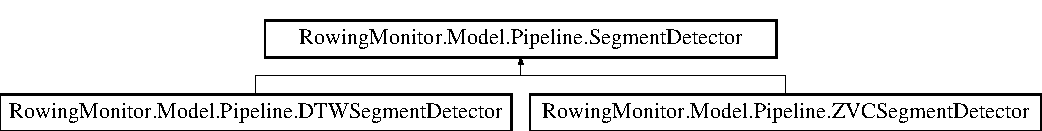
\includegraphics[height=1.755486cm]{class_rowing_monitor_1_1_model_1_1_pipeline_1_1_segment_detector}
\end{center}
\end{figure}
\subsection*{Public Member Functions}
\begin{DoxyCompactItemize}
\item 
delegate void \hyperlink{class_rowing_monitor_1_1_model_1_1_pipeline_1_1_segment_detector_aee5283f7fa49f68c5c4195449442093c}{Segment\+Detected\+Event\+Handler} (Object sender, \hyperlink{class_rowing_monitor_1_1_model_1_1_segment_detected_event_args}{Segment\+Detected\+Event\+Args} e)
\item 
abstract void \hyperlink{class_rowing_monitor_1_1_model_1_1_pipeline_1_1_segment_detector_a24dcb2926660a6218af3052f147d82da}{Update} (\hyperlink{struct_rowing_monitor_1_1_model_1_1_util_1_1_joint_data}{Joint\+Data} joint\+Data, Joint\+Type joint\+Type, String axis)
\item 
abstract List$<$ \hyperlink{struct_rowing_monitor_1_1_model_1_1_util_1_1_segment_hit}{Segment\+Hit} $>$ \hyperlink{class_rowing_monitor_1_1_model_1_1_pipeline_1_1_segment_detector_a28a3c23d7d350c0e37e9a58ff9a4e16b}{Detect} (\hyperlink{struct_rowing_monitor_1_1_model_1_1_util_1_1_joint_data}{Joint\+Data} joint\+Data, Joint\+Type joint\+Type, String axis)
\end{DoxyCompactItemize}
\subsection*{Protected Member Functions}
\begin{DoxyCompactItemize}
\item 
float \hyperlink{class_rowing_monitor_1_1_model_1_1_pipeline_1_1_segment_detector_a1f8ffebdfca18aa67a213ca817981161}{Get\+Joint\+Data\+Value} (\hyperlink{struct_rowing_monitor_1_1_model_1_1_util_1_1_joint_data}{Joint\+Data} joint\+Data, Joint\+Type joint\+Type, String axis)
\item 
virtual void \hyperlink{class_rowing_monitor_1_1_model_1_1_pipeline_1_1_segment_detector_a30d5b8752257a3992db11770506f6a8a}{On\+Segment\+Detected} (\hyperlink{class_rowing_monitor_1_1_model_1_1_segment_detected_event_args}{Segment\+Detected\+Event\+Args} e)
\end{DoxyCompactItemize}
\subsection*{Protected Attributes}
\begin{DoxyCompactItemize}
\item 
List$<$ \hyperlink{struct_rowing_monitor_1_1_model_1_1_util_1_1_segment_hit}{Segment\+Hit} $>$ \hyperlink{class_rowing_monitor_1_1_model_1_1_pipeline_1_1_segment_detector_a567492ea6e393bed7c946359cdf7c866}{hits} = new List$<$\hyperlink{struct_rowing_monitor_1_1_model_1_1_util_1_1_segment_hit}{Segment\+Hit}$>$()
\end{DoxyCompactItemize}
\subsection*{Properties}
\begin{DoxyCompactItemize}
\item 
Broadcast\+Block$<$ List$<$ \hyperlink{struct_rowing_monitor_1_1_model_1_1_util_1_1_segment_hit}{Segment\+Hit} $>$ $>$ \hyperlink{class_rowing_monitor_1_1_model_1_1_pipeline_1_1_segment_detector_a2f9933aa3e7251629d0b1676b73a336a}{Output}\hspace{0.3cm}{\ttfamily  \mbox{[}get, set\mbox{]}}
\item 
Joint\+Type \hyperlink{class_rowing_monitor_1_1_model_1_1_pipeline_1_1_segment_detector_a0bc85068e6ac401713535e38c0f1e18d}{Detection\+Joint\+Type}\hspace{0.3cm}{\ttfamily  \mbox{[}get, set\mbox{]}}
\item 
string \hyperlink{class_rowing_monitor_1_1_model_1_1_pipeline_1_1_segment_detector_ae8b2b75b70356efbe159de7427eb31fd}{Detection\+Axis}\hspace{0.3cm}{\ttfamily  \mbox{[}get, set\mbox{]}}
\item 
Action\+Block$<$ \hyperlink{struct_rowing_monitor_1_1_model_1_1_util_1_1_joint_data}{Joint\+Data} $>$ \hyperlink{class_rowing_monitor_1_1_model_1_1_pipeline_1_1_segment_detector_a1dff97a3144d7642595a8ce1fd4831a4}{Input}\hspace{0.3cm}{\ttfamily  \mbox{[}get, set\mbox{]}}
\end{DoxyCompactItemize}
\subsection*{Events}
\begin{DoxyCompactItemize}
\item 
\hyperlink{class_rowing_monitor_1_1_model_1_1_pipeline_1_1_segment_detector_aee5283f7fa49f68c5c4195449442093c}{Segment\+Detected\+Event\+Handler} \hyperlink{class_rowing_monitor_1_1_model_1_1_pipeline_1_1_segment_detector_aecedec106356c5d32e43e9c9471f12a3}{Segment\+Detected}
\end{DoxyCompactItemize}


\subsection{Member Function Documentation}
\mbox{\Hypertarget{class_rowing_monitor_1_1_model_1_1_pipeline_1_1_segment_detector_a28a3c23d7d350c0e37e9a58ff9a4e16b}\label{class_rowing_monitor_1_1_model_1_1_pipeline_1_1_segment_detector_a28a3c23d7d350c0e37e9a58ff9a4e16b}} 
\index{Rowing\+Monitor\+::\+Model\+::\+Pipeline\+::\+Segment\+Detector@{Rowing\+Monitor\+::\+Model\+::\+Pipeline\+::\+Segment\+Detector}!Detect@{Detect}}
\index{Detect@{Detect}!Rowing\+Monitor\+::\+Model\+::\+Pipeline\+::\+Segment\+Detector@{Rowing\+Monitor\+::\+Model\+::\+Pipeline\+::\+Segment\+Detector}}
\subsubsection{\texorpdfstring{Detect()}{Detect()}}
{\footnotesize\ttfamily abstract List$<$\hyperlink{struct_rowing_monitor_1_1_model_1_1_util_1_1_segment_hit}{Segment\+Hit}$>$ Rowing\+Monitor.\+Model.\+Pipeline.\+Segment\+Detector.\+Detect (\begin{DoxyParamCaption}\item[{\hyperlink{struct_rowing_monitor_1_1_model_1_1_util_1_1_joint_data}{Joint\+Data}}]{joint\+Data,  }\item[{Joint\+Type}]{joint\+Type,  }\item[{String}]{axis }\end{DoxyParamCaption})\hspace{0.3cm}{\ttfamily [pure virtual]}}

\mbox{\Hypertarget{class_rowing_monitor_1_1_model_1_1_pipeline_1_1_segment_detector_a1f8ffebdfca18aa67a213ca817981161}\label{class_rowing_monitor_1_1_model_1_1_pipeline_1_1_segment_detector_a1f8ffebdfca18aa67a213ca817981161}} 
\index{Rowing\+Monitor\+::\+Model\+::\+Pipeline\+::\+Segment\+Detector@{Rowing\+Monitor\+::\+Model\+::\+Pipeline\+::\+Segment\+Detector}!Get\+Joint\+Data\+Value@{Get\+Joint\+Data\+Value}}
\index{Get\+Joint\+Data\+Value@{Get\+Joint\+Data\+Value}!Rowing\+Monitor\+::\+Model\+::\+Pipeline\+::\+Segment\+Detector@{Rowing\+Monitor\+::\+Model\+::\+Pipeline\+::\+Segment\+Detector}}
\subsubsection{\texorpdfstring{Get\+Joint\+Data\+Value()}{GetJointDataValue()}}
{\footnotesize\ttfamily float Rowing\+Monitor.\+Model.\+Pipeline.\+Segment\+Detector.\+Get\+Joint\+Data\+Value (\begin{DoxyParamCaption}\item[{\hyperlink{struct_rowing_monitor_1_1_model_1_1_util_1_1_joint_data}{Joint\+Data}}]{joint\+Data,  }\item[{Joint\+Type}]{joint\+Type,  }\item[{String}]{axis }\end{DoxyParamCaption})\hspace{0.3cm}{\ttfamily [protected]}}

\mbox{\Hypertarget{class_rowing_monitor_1_1_model_1_1_pipeline_1_1_segment_detector_a30d5b8752257a3992db11770506f6a8a}\label{class_rowing_monitor_1_1_model_1_1_pipeline_1_1_segment_detector_a30d5b8752257a3992db11770506f6a8a}} 
\index{Rowing\+Monitor\+::\+Model\+::\+Pipeline\+::\+Segment\+Detector@{Rowing\+Monitor\+::\+Model\+::\+Pipeline\+::\+Segment\+Detector}!On\+Segment\+Detected@{On\+Segment\+Detected}}
\index{On\+Segment\+Detected@{On\+Segment\+Detected}!Rowing\+Monitor\+::\+Model\+::\+Pipeline\+::\+Segment\+Detector@{Rowing\+Monitor\+::\+Model\+::\+Pipeline\+::\+Segment\+Detector}}
\subsubsection{\texorpdfstring{On\+Segment\+Detected()}{OnSegmentDetected()}}
{\footnotesize\ttfamily virtual void Rowing\+Monitor.\+Model.\+Pipeline.\+Segment\+Detector.\+On\+Segment\+Detected (\begin{DoxyParamCaption}\item[{\hyperlink{class_rowing_monitor_1_1_model_1_1_segment_detected_event_args}{Segment\+Detected\+Event\+Args}}]{e }\end{DoxyParamCaption})\hspace{0.3cm}{\ttfamily [protected]}, {\ttfamily [virtual]}}



Reimplemented in \hyperlink{class_rowing_monitor_1_1_model_1_1_pipeline_1_1_z_v_c_segment_detector_a5eab838eda9f217722dfa05bc9d5095b}{Rowing\+Monitor.\+Model.\+Pipeline.\+Z\+V\+C\+Segment\+Detector}, and \hyperlink{class_rowing_monitor_1_1_model_1_1_pipeline_1_1_d_t_w_segment_detector_a6d2644f751e290cef82649c42becdd92}{Rowing\+Monitor.\+Model.\+Pipeline.\+D\+T\+W\+Segment\+Detector}.

\mbox{\Hypertarget{class_rowing_monitor_1_1_model_1_1_pipeline_1_1_segment_detector_aee5283f7fa49f68c5c4195449442093c}\label{class_rowing_monitor_1_1_model_1_1_pipeline_1_1_segment_detector_aee5283f7fa49f68c5c4195449442093c}} 
\index{Rowing\+Monitor\+::\+Model\+::\+Pipeline\+::\+Segment\+Detector@{Rowing\+Monitor\+::\+Model\+::\+Pipeline\+::\+Segment\+Detector}!Segment\+Detected\+Event\+Handler@{Segment\+Detected\+Event\+Handler}}
\index{Segment\+Detected\+Event\+Handler@{Segment\+Detected\+Event\+Handler}!Rowing\+Monitor\+::\+Model\+::\+Pipeline\+::\+Segment\+Detector@{Rowing\+Monitor\+::\+Model\+::\+Pipeline\+::\+Segment\+Detector}}
\subsubsection{\texorpdfstring{Segment\+Detected\+Event\+Handler()}{SegmentDetectedEventHandler()}}
{\footnotesize\ttfamily delegate void Rowing\+Monitor.\+Model.\+Pipeline.\+Segment\+Detector.\+Segment\+Detected\+Event\+Handler (\begin{DoxyParamCaption}\item[{Object}]{sender,  }\item[{\hyperlink{class_rowing_monitor_1_1_model_1_1_segment_detected_event_args}{Segment\+Detected\+Event\+Args}}]{e }\end{DoxyParamCaption})}

\mbox{\Hypertarget{class_rowing_monitor_1_1_model_1_1_pipeline_1_1_segment_detector_a24dcb2926660a6218af3052f147d82da}\label{class_rowing_monitor_1_1_model_1_1_pipeline_1_1_segment_detector_a24dcb2926660a6218af3052f147d82da}} 
\index{Rowing\+Monitor\+::\+Model\+::\+Pipeline\+::\+Segment\+Detector@{Rowing\+Monitor\+::\+Model\+::\+Pipeline\+::\+Segment\+Detector}!Update@{Update}}
\index{Update@{Update}!Rowing\+Monitor\+::\+Model\+::\+Pipeline\+::\+Segment\+Detector@{Rowing\+Monitor\+::\+Model\+::\+Pipeline\+::\+Segment\+Detector}}
\subsubsection{\texorpdfstring{Update()}{Update()}}
{\footnotesize\ttfamily abstract void Rowing\+Monitor.\+Model.\+Pipeline.\+Segment\+Detector.\+Update (\begin{DoxyParamCaption}\item[{\hyperlink{struct_rowing_monitor_1_1_model_1_1_util_1_1_joint_data}{Joint\+Data}}]{joint\+Data,  }\item[{Joint\+Type}]{joint\+Type,  }\item[{String}]{axis }\end{DoxyParamCaption})\hspace{0.3cm}{\ttfamily [pure virtual]}}



Implemented in \hyperlink{class_rowing_monitor_1_1_model_1_1_pipeline_1_1_z_v_c_segment_detector_a81c28e4ede1561c2fe1eca29f63f0767}{Rowing\+Monitor.\+Model.\+Pipeline.\+Z\+V\+C\+Segment\+Detector}.



\subsection{Member Data Documentation}
\mbox{\Hypertarget{class_rowing_monitor_1_1_model_1_1_pipeline_1_1_segment_detector_a567492ea6e393bed7c946359cdf7c866}\label{class_rowing_monitor_1_1_model_1_1_pipeline_1_1_segment_detector_a567492ea6e393bed7c946359cdf7c866}} 
\index{Rowing\+Monitor\+::\+Model\+::\+Pipeline\+::\+Segment\+Detector@{Rowing\+Monitor\+::\+Model\+::\+Pipeline\+::\+Segment\+Detector}!hits@{hits}}
\index{hits@{hits}!Rowing\+Monitor\+::\+Model\+::\+Pipeline\+::\+Segment\+Detector@{Rowing\+Monitor\+::\+Model\+::\+Pipeline\+::\+Segment\+Detector}}
\subsubsection{\texorpdfstring{hits}{hits}}
{\footnotesize\ttfamily List$<$\hyperlink{struct_rowing_monitor_1_1_model_1_1_util_1_1_segment_hit}{Segment\+Hit}$>$ Rowing\+Monitor.\+Model.\+Pipeline.\+Segment\+Detector.\+hits = new List$<$\hyperlink{struct_rowing_monitor_1_1_model_1_1_util_1_1_segment_hit}{Segment\+Hit}$>$()\hspace{0.3cm}{\ttfamily [protected]}}



\subsection{Property Documentation}
\mbox{\Hypertarget{class_rowing_monitor_1_1_model_1_1_pipeline_1_1_segment_detector_ae8b2b75b70356efbe159de7427eb31fd}\label{class_rowing_monitor_1_1_model_1_1_pipeline_1_1_segment_detector_ae8b2b75b70356efbe159de7427eb31fd}} 
\index{Rowing\+Monitor\+::\+Model\+::\+Pipeline\+::\+Segment\+Detector@{Rowing\+Monitor\+::\+Model\+::\+Pipeline\+::\+Segment\+Detector}!Detection\+Axis@{Detection\+Axis}}
\index{Detection\+Axis@{Detection\+Axis}!Rowing\+Monitor\+::\+Model\+::\+Pipeline\+::\+Segment\+Detector@{Rowing\+Monitor\+::\+Model\+::\+Pipeline\+::\+Segment\+Detector}}
\subsubsection{\texorpdfstring{Detection\+Axis}{DetectionAxis}}
{\footnotesize\ttfamily string Rowing\+Monitor.\+Model.\+Pipeline.\+Segment\+Detector.\+Detection\+Axis\hspace{0.3cm}{\ttfamily [get]}, {\ttfamily [set]}}

\mbox{\Hypertarget{class_rowing_monitor_1_1_model_1_1_pipeline_1_1_segment_detector_a0bc85068e6ac401713535e38c0f1e18d}\label{class_rowing_monitor_1_1_model_1_1_pipeline_1_1_segment_detector_a0bc85068e6ac401713535e38c0f1e18d}} 
\index{Rowing\+Monitor\+::\+Model\+::\+Pipeline\+::\+Segment\+Detector@{Rowing\+Monitor\+::\+Model\+::\+Pipeline\+::\+Segment\+Detector}!Detection\+Joint\+Type@{Detection\+Joint\+Type}}
\index{Detection\+Joint\+Type@{Detection\+Joint\+Type}!Rowing\+Monitor\+::\+Model\+::\+Pipeline\+::\+Segment\+Detector@{Rowing\+Monitor\+::\+Model\+::\+Pipeline\+::\+Segment\+Detector}}
\subsubsection{\texorpdfstring{Detection\+Joint\+Type}{DetectionJointType}}
{\footnotesize\ttfamily Joint\+Type Rowing\+Monitor.\+Model.\+Pipeline.\+Segment\+Detector.\+Detection\+Joint\+Type\hspace{0.3cm}{\ttfamily [get]}, {\ttfamily [set]}}

\mbox{\Hypertarget{class_rowing_monitor_1_1_model_1_1_pipeline_1_1_segment_detector_a1dff97a3144d7642595a8ce1fd4831a4}\label{class_rowing_monitor_1_1_model_1_1_pipeline_1_1_segment_detector_a1dff97a3144d7642595a8ce1fd4831a4}} 
\index{Rowing\+Monitor\+::\+Model\+::\+Pipeline\+::\+Segment\+Detector@{Rowing\+Monitor\+::\+Model\+::\+Pipeline\+::\+Segment\+Detector}!Input@{Input}}
\index{Input@{Input}!Rowing\+Monitor\+::\+Model\+::\+Pipeline\+::\+Segment\+Detector@{Rowing\+Monitor\+::\+Model\+::\+Pipeline\+::\+Segment\+Detector}}
\subsubsection{\texorpdfstring{Input}{Input}}
{\footnotesize\ttfamily Action\+Block$<$\hyperlink{struct_rowing_monitor_1_1_model_1_1_util_1_1_joint_data}{Joint\+Data}$>$ Rowing\+Monitor.\+Model.\+Pipeline.\+Segment\+Detector.\+Input\hspace{0.3cm}{\ttfamily [get]}, {\ttfamily [set]}}

\mbox{\Hypertarget{class_rowing_monitor_1_1_model_1_1_pipeline_1_1_segment_detector_a2f9933aa3e7251629d0b1676b73a336a}\label{class_rowing_monitor_1_1_model_1_1_pipeline_1_1_segment_detector_a2f9933aa3e7251629d0b1676b73a336a}} 
\index{Rowing\+Monitor\+::\+Model\+::\+Pipeline\+::\+Segment\+Detector@{Rowing\+Monitor\+::\+Model\+::\+Pipeline\+::\+Segment\+Detector}!Output@{Output}}
\index{Output@{Output}!Rowing\+Monitor\+::\+Model\+::\+Pipeline\+::\+Segment\+Detector@{Rowing\+Monitor\+::\+Model\+::\+Pipeline\+::\+Segment\+Detector}}
\subsubsection{\texorpdfstring{Output}{Output}}
{\footnotesize\ttfamily Broadcast\+Block$<$List$<$\hyperlink{struct_rowing_monitor_1_1_model_1_1_util_1_1_segment_hit}{Segment\+Hit}$>$ $>$ Rowing\+Monitor.\+Model.\+Pipeline.\+Segment\+Detector.\+Output\hspace{0.3cm}{\ttfamily [get]}, {\ttfamily [set]}}



\subsection{Event Documentation}
\mbox{\Hypertarget{class_rowing_monitor_1_1_model_1_1_pipeline_1_1_segment_detector_aecedec106356c5d32e43e9c9471f12a3}\label{class_rowing_monitor_1_1_model_1_1_pipeline_1_1_segment_detector_aecedec106356c5d32e43e9c9471f12a3}} 
\index{Rowing\+Monitor\+::\+Model\+::\+Pipeline\+::\+Segment\+Detector@{Rowing\+Monitor\+::\+Model\+::\+Pipeline\+::\+Segment\+Detector}!Segment\+Detected@{Segment\+Detected}}
\index{Segment\+Detected@{Segment\+Detected}!Rowing\+Monitor\+::\+Model\+::\+Pipeline\+::\+Segment\+Detector@{Rowing\+Monitor\+::\+Model\+::\+Pipeline\+::\+Segment\+Detector}}
\subsubsection{\texorpdfstring{Segment\+Detected}{SegmentDetected}}
{\footnotesize\ttfamily \hyperlink{class_rowing_monitor_1_1_model_1_1_pipeline_1_1_segment_detector_aee5283f7fa49f68c5c4195449442093c}{Segment\+Detected\+Event\+Handler} Rowing\+Monitor.\+Model.\+Pipeline.\+Segment\+Detector.\+Segment\+Detected}



The documentation for this class was generated from the following file\+:\begin{DoxyCompactItemize}
\item 
Model/\+Pipeline/\hyperlink{_segment_detector_8cs}{Segment\+Detector.\+cs}\end{DoxyCompactItemize}

\hypertarget{struct_rowing_monitor_1_1_model_1_1_util_1_1_segment_hit}{}\section{Rowing\+Monitor.\+Model.\+Util.\+Segment\+Hit Struct Reference}
\label{struct_rowing_monitor_1_1_model_1_1_util_1_1_segment_hit}\index{Rowing\+Monitor.\+Model.\+Util.\+Segment\+Hit@{Rowing\+Monitor.\+Model.\+Util.\+Segment\+Hit}}
\subsection*{Properties}
\begin{DoxyCompactItemize}
\item 
long \hyperlink{struct_rowing_monitor_1_1_model_1_1_util_1_1_segment_hit_aaf855f224da3b43af2ea5f7896914efb}{Index}\hspace{0.3cm}{\ttfamily  \mbox{[}get, set\mbox{]}}
\begin{DoxyCompactList}\small\item\em Index of the joint data that this hit belongs to. \end{DoxyCompactList}\item 
long \hyperlink{struct_rowing_monitor_1_1_model_1_1_util_1_1_segment_hit_ad943df68e8adfeaa2b76701701cef0df}{Detection\+Index}\hspace{0.3cm}{\ttfamily  \mbox{[}get, set\mbox{]}}
\begin{DoxyCompactList}\small\item\em Index of the joint data where this hit was detected. \end{DoxyCompactList}\item 
double \hyperlink{struct_rowing_monitor_1_1_model_1_1_util_1_1_segment_hit_ab40df6a59087cfd176f989111279a5e2}{Abs\+Timestamp}\hspace{0.3cm}{\ttfamily  \mbox{[}get, set\mbox{]}}
\begin{DoxyCompactList}\small\item\em Absolute timestamp of the joint data that this hit belongs to. \end{DoxyCompactList}\item 
double \hyperlink{struct_rowing_monitor_1_1_model_1_1_util_1_1_segment_hit_ab9778fc572f014c1d75de5898f8c83d2}{Detection\+Abs\+Timestamp}\hspace{0.3cm}{\ttfamily  \mbox{[}get, set\mbox{]}}
\begin{DoxyCompactList}\small\item\em Absolute timestamp of the joint data where this hit was detected. \end{DoxyCompactList}\item 
\hyperlink{namespace_rowing_monitor_1_1_model_1_1_util_a7135d50f11f02e6f0cb9680dc68dba56}{Hit\+Type} \hyperlink{struct_rowing_monitor_1_1_model_1_1_util_1_1_segment_hit_ab2a359ba79fbc8456596219484f2a159}{Hit\+Type}\hspace{0.3cm}{\ttfamily  \mbox{[}get, set\mbox{]}}
\begin{DoxyCompactList}\small\item\em Type of this hit in the context of a segment. \end{DoxyCompactList}\end{DoxyCompactItemize}


\subsection{Property Documentation}
\mbox{\Hypertarget{struct_rowing_monitor_1_1_model_1_1_util_1_1_segment_hit_ab40df6a59087cfd176f989111279a5e2}\label{struct_rowing_monitor_1_1_model_1_1_util_1_1_segment_hit_ab40df6a59087cfd176f989111279a5e2}} 
\index{Rowing\+Monitor\+::\+Model\+::\+Util\+::\+Segment\+Hit@{Rowing\+Monitor\+::\+Model\+::\+Util\+::\+Segment\+Hit}!Abs\+Timestamp@{Abs\+Timestamp}}
\index{Abs\+Timestamp@{Abs\+Timestamp}!Rowing\+Monitor\+::\+Model\+::\+Util\+::\+Segment\+Hit@{Rowing\+Monitor\+::\+Model\+::\+Util\+::\+Segment\+Hit}}
\subsubsection{\texorpdfstring{Abs\+Timestamp}{AbsTimestamp}}
{\footnotesize\ttfamily double Rowing\+Monitor.\+Model.\+Util.\+Segment\+Hit.\+Abs\+Timestamp\hspace{0.3cm}{\ttfamily [get]}, {\ttfamily [set]}}



Absolute timestamp of the joint data that this hit belongs to. 

\mbox{\Hypertarget{struct_rowing_monitor_1_1_model_1_1_util_1_1_segment_hit_ab9778fc572f014c1d75de5898f8c83d2}\label{struct_rowing_monitor_1_1_model_1_1_util_1_1_segment_hit_ab9778fc572f014c1d75de5898f8c83d2}} 
\index{Rowing\+Monitor\+::\+Model\+::\+Util\+::\+Segment\+Hit@{Rowing\+Monitor\+::\+Model\+::\+Util\+::\+Segment\+Hit}!Detection\+Abs\+Timestamp@{Detection\+Abs\+Timestamp}}
\index{Detection\+Abs\+Timestamp@{Detection\+Abs\+Timestamp}!Rowing\+Monitor\+::\+Model\+::\+Util\+::\+Segment\+Hit@{Rowing\+Monitor\+::\+Model\+::\+Util\+::\+Segment\+Hit}}
\subsubsection{\texorpdfstring{Detection\+Abs\+Timestamp}{DetectionAbsTimestamp}}
{\footnotesize\ttfamily double Rowing\+Monitor.\+Model.\+Util.\+Segment\+Hit.\+Detection\+Abs\+Timestamp\hspace{0.3cm}{\ttfamily [get]}, {\ttfamily [set]}}



Absolute timestamp of the joint data where this hit was detected. 

\mbox{\Hypertarget{struct_rowing_monitor_1_1_model_1_1_util_1_1_segment_hit_ad943df68e8adfeaa2b76701701cef0df}\label{struct_rowing_monitor_1_1_model_1_1_util_1_1_segment_hit_ad943df68e8adfeaa2b76701701cef0df}} 
\index{Rowing\+Monitor\+::\+Model\+::\+Util\+::\+Segment\+Hit@{Rowing\+Monitor\+::\+Model\+::\+Util\+::\+Segment\+Hit}!Detection\+Index@{Detection\+Index}}
\index{Detection\+Index@{Detection\+Index}!Rowing\+Monitor\+::\+Model\+::\+Util\+::\+Segment\+Hit@{Rowing\+Monitor\+::\+Model\+::\+Util\+::\+Segment\+Hit}}
\subsubsection{\texorpdfstring{Detection\+Index}{DetectionIndex}}
{\footnotesize\ttfamily long Rowing\+Monitor.\+Model.\+Util.\+Segment\+Hit.\+Detection\+Index\hspace{0.3cm}{\ttfamily [get]}, {\ttfamily [set]}}



Index of the joint data where this hit was detected. 

\mbox{\Hypertarget{struct_rowing_monitor_1_1_model_1_1_util_1_1_segment_hit_ab2a359ba79fbc8456596219484f2a159}\label{struct_rowing_monitor_1_1_model_1_1_util_1_1_segment_hit_ab2a359ba79fbc8456596219484f2a159}} 
\index{Rowing\+Monitor\+::\+Model\+::\+Util\+::\+Segment\+Hit@{Rowing\+Monitor\+::\+Model\+::\+Util\+::\+Segment\+Hit}!Hit\+Type@{Hit\+Type}}
\index{Hit\+Type@{Hit\+Type}!Rowing\+Monitor\+::\+Model\+::\+Util\+::\+Segment\+Hit@{Rowing\+Monitor\+::\+Model\+::\+Util\+::\+Segment\+Hit}}
\subsubsection{\texorpdfstring{Hit\+Type}{HitType}}
{\footnotesize\ttfamily \hyperlink{namespace_rowing_monitor_1_1_model_1_1_util_a7135d50f11f02e6f0cb9680dc68dba56}{Hit\+Type} Rowing\+Monitor.\+Model.\+Util.\+Segment\+Hit.\+Hit\+Type\hspace{0.3cm}{\ttfamily [get]}, {\ttfamily [set]}}



Type of this hit in the context of a segment. 

\mbox{\Hypertarget{struct_rowing_monitor_1_1_model_1_1_util_1_1_segment_hit_aaf855f224da3b43af2ea5f7896914efb}\label{struct_rowing_monitor_1_1_model_1_1_util_1_1_segment_hit_aaf855f224da3b43af2ea5f7896914efb}} 
\index{Rowing\+Monitor\+::\+Model\+::\+Util\+::\+Segment\+Hit@{Rowing\+Monitor\+::\+Model\+::\+Util\+::\+Segment\+Hit}!Index@{Index}}
\index{Index@{Index}!Rowing\+Monitor\+::\+Model\+::\+Util\+::\+Segment\+Hit@{Rowing\+Monitor\+::\+Model\+::\+Util\+::\+Segment\+Hit}}
\subsubsection{\texorpdfstring{Index}{Index}}
{\footnotesize\ttfamily long Rowing\+Monitor.\+Model.\+Util.\+Segment\+Hit.\+Index\hspace{0.3cm}{\ttfamily [get]}, {\ttfamily [set]}}



Index of the joint data that this hit belongs to. 



The documentation for this struct was generated from the following file\+:\begin{DoxyCompactItemize}
\item 
Model/\+Util/\hyperlink{_kinect_data_handler_8cs}{Kinect\+Data\+Handler.\+cs}\end{DoxyCompactItemize}

\hypertarget{class_rowing_monitor_1_1_model_1_1_util_1_1_segment_hit_handler}{}\section{Rowing\+Monitor.\+Model.\+Util.\+Segment\+Hit\+Handler Class Reference}
\label{class_rowing_monitor_1_1_model_1_1_util_1_1_segment_hit_handler}\index{Rowing\+Monitor.\+Model.\+Util.\+Segment\+Hit\+Handler@{Rowing\+Monitor.\+Model.\+Util.\+Segment\+Hit\+Handler}}
\subsection*{Static Public Member Functions}
\begin{DoxyCompactItemize}
\item 
static bool \hyperlink{class_rowing_monitor_1_1_model_1_1_util_1_1_segment_hit_handler_adbd44130a8d894cd7c21430c3eedf9e1}{Check\+If\+New\+Segment\+Started} (List$<$ \hyperlink{struct_rowing_monitor_1_1_model_1_1_util_1_1_segment_hit}{Segment\+Hit} $>$ hits)
\item 
static long \mbox{[}$\,$\mbox{]} \hyperlink{class_rowing_monitor_1_1_model_1_1_util_1_1_segment_hit_handler_a75d8b23514da843ef1eebf9e684f8094}{Get\+Last\+Segment\+Start\+End} (List$<$ \hyperlink{struct_rowing_monitor_1_1_model_1_1_util_1_1_segment_hit}{Segment\+Hit} $>$ hits)
\begin{DoxyCompactList}\small\item\em Return the bounding indices values of the last complete segment. \end{DoxyCompactList}\item 
static long \hyperlink{class_rowing_monitor_1_1_model_1_1_util_1_1_segment_hit_handler_ac73a1aebbe85844658b84fd48591c302}{Get\+Last\+Segment\+Internal} (List$<$ \hyperlink{struct_rowing_monitor_1_1_model_1_1_util_1_1_segment_hit}{Segment\+Hit} $>$ hits)
\begin{DoxyCompactList}\small\item\em Returns the index of the last detected internal segment hit. \end{DoxyCompactList}\end{DoxyCompactItemize}


\subsection{Member Function Documentation}
\mbox{\Hypertarget{class_rowing_monitor_1_1_model_1_1_util_1_1_segment_hit_handler_adbd44130a8d894cd7c21430c3eedf9e1}\label{class_rowing_monitor_1_1_model_1_1_util_1_1_segment_hit_handler_adbd44130a8d894cd7c21430c3eedf9e1}} 
\index{Rowing\+Monitor\+::\+Model\+::\+Util\+::\+Segment\+Hit\+Handler@{Rowing\+Monitor\+::\+Model\+::\+Util\+::\+Segment\+Hit\+Handler}!Check\+If\+New\+Segment\+Started@{Check\+If\+New\+Segment\+Started}}
\index{Check\+If\+New\+Segment\+Started@{Check\+If\+New\+Segment\+Started}!Rowing\+Monitor\+::\+Model\+::\+Util\+::\+Segment\+Hit\+Handler@{Rowing\+Monitor\+::\+Model\+::\+Util\+::\+Segment\+Hit\+Handler}}
\subsubsection{\texorpdfstring{Check\+If\+New\+Segment\+Started()}{CheckIfNewSegmentStarted()}}
{\footnotesize\ttfamily static bool Rowing\+Monitor.\+Model.\+Util.\+Segment\+Hit\+Handler.\+Check\+If\+New\+Segment\+Started (\begin{DoxyParamCaption}\item[{List$<$ \hyperlink{struct_rowing_monitor_1_1_model_1_1_util_1_1_segment_hit}{Segment\+Hit} $>$}]{hits }\end{DoxyParamCaption})\hspace{0.3cm}{\ttfamily [static]}}

\mbox{\Hypertarget{class_rowing_monitor_1_1_model_1_1_util_1_1_segment_hit_handler_ac73a1aebbe85844658b84fd48591c302}\label{class_rowing_monitor_1_1_model_1_1_util_1_1_segment_hit_handler_ac73a1aebbe85844658b84fd48591c302}} 
\index{Rowing\+Monitor\+::\+Model\+::\+Util\+::\+Segment\+Hit\+Handler@{Rowing\+Monitor\+::\+Model\+::\+Util\+::\+Segment\+Hit\+Handler}!Get\+Last\+Segment\+Internal@{Get\+Last\+Segment\+Internal}}
\index{Get\+Last\+Segment\+Internal@{Get\+Last\+Segment\+Internal}!Rowing\+Monitor\+::\+Model\+::\+Util\+::\+Segment\+Hit\+Handler@{Rowing\+Monitor\+::\+Model\+::\+Util\+::\+Segment\+Hit\+Handler}}
\subsubsection{\texorpdfstring{Get\+Last\+Segment\+Internal()}{GetLastSegmentInternal()}}
{\footnotesize\ttfamily static long Rowing\+Monitor.\+Model.\+Util.\+Segment\+Hit\+Handler.\+Get\+Last\+Segment\+Internal (\begin{DoxyParamCaption}\item[{List$<$ \hyperlink{struct_rowing_monitor_1_1_model_1_1_util_1_1_segment_hit}{Segment\+Hit} $>$}]{hits }\end{DoxyParamCaption})\hspace{0.3cm}{\ttfamily [static]}}



Returns the index of the last detected internal segment hit. 


\begin{DoxyParams}{Parameters}
{\em hits} & List of detected hits.\\
\hline
\end{DoxyParams}
\begin{DoxyReturn}{Returns}
Index of last detected internal segment hit.
\end{DoxyReturn}
\mbox{\Hypertarget{class_rowing_monitor_1_1_model_1_1_util_1_1_segment_hit_handler_a75d8b23514da843ef1eebf9e684f8094}\label{class_rowing_monitor_1_1_model_1_1_util_1_1_segment_hit_handler_a75d8b23514da843ef1eebf9e684f8094}} 
\index{Rowing\+Monitor\+::\+Model\+::\+Util\+::\+Segment\+Hit\+Handler@{Rowing\+Monitor\+::\+Model\+::\+Util\+::\+Segment\+Hit\+Handler}!Get\+Last\+Segment\+Start\+End@{Get\+Last\+Segment\+Start\+End}}
\index{Get\+Last\+Segment\+Start\+End@{Get\+Last\+Segment\+Start\+End}!Rowing\+Monitor\+::\+Model\+::\+Util\+::\+Segment\+Hit\+Handler@{Rowing\+Monitor\+::\+Model\+::\+Util\+::\+Segment\+Hit\+Handler}}
\subsubsection{\texorpdfstring{Get\+Last\+Segment\+Start\+End()}{GetLastSegmentStartEnd()}}
{\footnotesize\ttfamily static long \mbox{[}$\,$\mbox{]} Rowing\+Monitor.\+Model.\+Util.\+Segment\+Hit\+Handler.\+Get\+Last\+Segment\+Start\+End (\begin{DoxyParamCaption}\item[{List$<$ \hyperlink{struct_rowing_monitor_1_1_model_1_1_util_1_1_segment_hit}{Segment\+Hit} $>$}]{hits }\end{DoxyParamCaption})\hspace{0.3cm}{\ttfamily [static]}}



Return the bounding indices values of the last complete segment. 


\begin{DoxyParams}{Parameters}
{\em hits} & List of detected hits.\\
\hline
\end{DoxyParams}
\begin{DoxyReturn}{Returns}
Start an d end index of the lastdetected segment.
\end{DoxyReturn}


The documentation for this class was generated from the following file\+:\begin{DoxyCompactItemize}
\item 
Model/\+Util/\hyperlink{_segment_hit_handler_8cs}{Segment\+Hit\+Handler.\+cs}\end{DoxyCompactItemize}

\hypertarget{class_rowing_monitor_1_1_model_1_1_shifted_frame_arrived_event_args}{}\section{Rowing\+Monitor.\+Model.\+Shifted\+Frame\+Arrived\+Event\+Args Class Reference}
\label{class_rowing_monitor_1_1_model_1_1_shifted_frame_arrived_event_args}\index{Rowing\+Monitor.\+Model.\+Shifted\+Frame\+Arrived\+Event\+Args@{Rowing\+Monitor.\+Model.\+Shifted\+Frame\+Arrived\+Event\+Args}}


Represents the arguments for a shifted frame arrived event.  


Inheritance diagram for Rowing\+Monitor.\+Model.\+Shifted\+Frame\+Arrived\+Event\+Args\+:\begin{figure}[H]
\begin{center}
\leavevmode
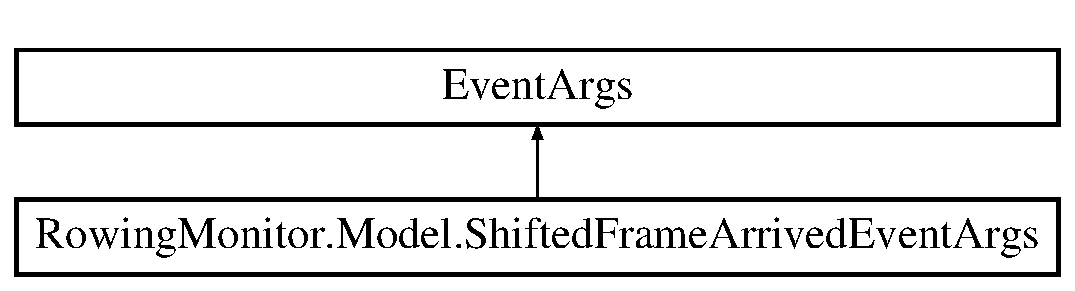
\includegraphics[height=2.000000cm]{class_rowing_monitor_1_1_model_1_1_shifted_frame_arrived_event_args}
\end{center}
\end{figure}
\subsection*{Public Member Functions}
\begin{DoxyCompactItemize}
\item 
\hyperlink{class_rowing_monitor_1_1_model_1_1_shifted_frame_arrived_event_args_a7ea2f2cc785f346a8fc51e770352ef2c}{Shifted\+Frame\+Arrived\+Event\+Args} (\hyperlink{struct_rowing_monitor_1_1_model_1_1_util_1_1_joint_data}{Joint\+Data} shifted\+Joint\+Data)
\end{DoxyCompactItemize}
\subsection*{Properties}
\begin{DoxyCompactItemize}
\item 
\hyperlink{struct_rowing_monitor_1_1_model_1_1_util_1_1_joint_data}{Joint\+Data} \hyperlink{class_rowing_monitor_1_1_model_1_1_shifted_frame_arrived_event_args_a668747182e00705fcaef8d16320ce730}{Shifted\+Joint\+Data}\hspace{0.3cm}{\ttfamily  \mbox{[}get\mbox{]}}
\end{DoxyCompactItemize}


\subsection{Detailed Description}
Represents the arguments for a shifted frame arrived event. 



\subsection{Constructor \& Destructor Documentation}
\mbox{\Hypertarget{class_rowing_monitor_1_1_model_1_1_shifted_frame_arrived_event_args_a7ea2f2cc785f346a8fc51e770352ef2c}\label{class_rowing_monitor_1_1_model_1_1_shifted_frame_arrived_event_args_a7ea2f2cc785f346a8fc51e770352ef2c}} 
\index{Rowing\+Monitor\+::\+Model\+::\+Shifted\+Frame\+Arrived\+Event\+Args@{Rowing\+Monitor\+::\+Model\+::\+Shifted\+Frame\+Arrived\+Event\+Args}!Shifted\+Frame\+Arrived\+Event\+Args@{Shifted\+Frame\+Arrived\+Event\+Args}}
\index{Shifted\+Frame\+Arrived\+Event\+Args@{Shifted\+Frame\+Arrived\+Event\+Args}!Rowing\+Monitor\+::\+Model\+::\+Shifted\+Frame\+Arrived\+Event\+Args@{Rowing\+Monitor\+::\+Model\+::\+Shifted\+Frame\+Arrived\+Event\+Args}}
\subsubsection{\texorpdfstring{Shifted\+Frame\+Arrived\+Event\+Args()}{ShiftedFrameArrivedEventArgs()}}
{\footnotesize\ttfamily Rowing\+Monitor.\+Model.\+Shifted\+Frame\+Arrived\+Event\+Args.\+Shifted\+Frame\+Arrived\+Event\+Args (\begin{DoxyParamCaption}\item[{\hyperlink{struct_rowing_monitor_1_1_model_1_1_util_1_1_joint_data}{Joint\+Data}}]{shifted\+Joint\+Data }\end{DoxyParamCaption})}



\subsection{Property Documentation}
\mbox{\Hypertarget{class_rowing_monitor_1_1_model_1_1_shifted_frame_arrived_event_args_a668747182e00705fcaef8d16320ce730}\label{class_rowing_monitor_1_1_model_1_1_shifted_frame_arrived_event_args_a668747182e00705fcaef8d16320ce730}} 
\index{Rowing\+Monitor\+::\+Model\+::\+Shifted\+Frame\+Arrived\+Event\+Args@{Rowing\+Monitor\+::\+Model\+::\+Shifted\+Frame\+Arrived\+Event\+Args}!Shifted\+Joint\+Data@{Shifted\+Joint\+Data}}
\index{Shifted\+Joint\+Data@{Shifted\+Joint\+Data}!Rowing\+Monitor\+::\+Model\+::\+Shifted\+Frame\+Arrived\+Event\+Args@{Rowing\+Monitor\+::\+Model\+::\+Shifted\+Frame\+Arrived\+Event\+Args}}
\subsubsection{\texorpdfstring{Shifted\+Joint\+Data}{ShiftedJointData}}
{\footnotesize\ttfamily \hyperlink{struct_rowing_monitor_1_1_model_1_1_util_1_1_joint_data}{Joint\+Data} Rowing\+Monitor.\+Model.\+Shifted\+Frame\+Arrived\+Event\+Args.\+Shifted\+Joint\+Data\hspace{0.3cm}{\ttfamily [get]}}



The documentation for this class was generated from the following file\+:\begin{DoxyCompactItemize}
\item 
Model/\+Event\+Args/\hyperlink{_shifted_frame_arrived_event_args_8cs}{Shifted\+Frame\+Arrived\+Event\+Args.\+cs}\end{DoxyCompactItemize}

\hypertarget{class_rowing_monitor_1_1_model_1_1_pipeline_1_1_shifter}{}\section{Rowing\+Monitor.\+Model.\+Pipeline.\+Shifter Class Reference}
\label{class_rowing_monitor_1_1_model_1_1_pipeline_1_1_shifter}\index{Rowing\+Monitor.\+Model.\+Pipeline.\+Shifter@{Rowing\+Monitor.\+Model.\+Pipeline.\+Shifter}}


Shifts the origin to the middle point between the foot joints plus an offset from foot to hip joint. Also rotates all joints until origin and hip joint form a horizontal line.  


\subsection*{Public Member Functions}
\begin{DoxyCompactItemize}
\item 
delegate void \hyperlink{class_rowing_monitor_1_1_model_1_1_pipeline_1_1_shifter_a348927ce21661a1658060d083a91bd61}{Shifted\+Frame\+Arrived\+Event\+Handler} (Object sender, \hyperlink{class_rowing_monitor_1_1_model_1_1_shifted_frame_arrived_event_args}{Shifted\+Frame\+Arrived\+Event\+Args} e)
\item 
\hyperlink{class_rowing_monitor_1_1_model_1_1_pipeline_1_1_shifter_a22e7862fcbc55f78166971743aba7a94}{Shifter} ()
\item 
\hyperlink{struct_rowing_monitor_1_1_model_1_1_util_1_1_joint_data}{Joint\+Data} \hyperlink{class_rowing_monitor_1_1_model_1_1_pipeline_1_1_shifter_ac48bc7448590a3926823feb882fa9042}{Shift\+And\+Rotate} (\hyperlink{struct_rowing_monitor_1_1_model_1_1_util_1_1_joint_data}{Joint\+Data} joint\+Data)
\item 
void \hyperlink{class_rowing_monitor_1_1_model_1_1_pipeline_1_1_shifter_ae34f476a6eee98adea44c3e0e72d6e70}{Updata} (\hyperlink{struct_rowing_monitor_1_1_model_1_1_util_1_1_joint_data}{Joint\+Data} joint\+Data)
\end{DoxyCompactItemize}
\subsection*{Properties}
\begin{DoxyCompactItemize}
\item 
Broadcast\+Block$<$ \hyperlink{struct_rowing_monitor_1_1_model_1_1_util_1_1_joint_data}{Joint\+Data} $>$ \hyperlink{class_rowing_monitor_1_1_model_1_1_pipeline_1_1_shifter_a6d1edcd6586e11141863498c7bddfc13}{Output}\hspace{0.3cm}{\ttfamily  \mbox{[}get, set\mbox{]}}
\item 
Action\+Block$<$ \hyperlink{struct_rowing_monitor_1_1_model_1_1_util_1_1_joint_data}{Joint\+Data} $>$ \hyperlink{class_rowing_monitor_1_1_model_1_1_pipeline_1_1_shifter_aa404f3bb229b6f57e5144f2a5c67bb43}{Input}\hspace{0.3cm}{\ttfamily  \mbox{[}get, set\mbox{]}}
\end{DoxyCompactItemize}
\subsection*{Events}
\begin{DoxyCompactItemize}
\item 
\hyperlink{class_rowing_monitor_1_1_model_1_1_pipeline_1_1_shifter_a348927ce21661a1658060d083a91bd61}{Shifted\+Frame\+Arrived\+Event\+Handler} \hyperlink{class_rowing_monitor_1_1_model_1_1_pipeline_1_1_shifter_afd44d987e237cb912776101166c9f14f}{Shifted\+Frame\+Arrived}
\end{DoxyCompactItemize}


\subsection{Detailed Description}
Shifts the origin to the middle point between the foot joints plus an offset from foot to hip joint. Also rotates all joints until origin and hip joint form a horizontal line. 



\subsection{Constructor \& Destructor Documentation}
\mbox{\Hypertarget{class_rowing_monitor_1_1_model_1_1_pipeline_1_1_shifter_a22e7862fcbc55f78166971743aba7a94}\label{class_rowing_monitor_1_1_model_1_1_pipeline_1_1_shifter_a22e7862fcbc55f78166971743aba7a94}} 
\index{Rowing\+Monitor\+::\+Model\+::\+Pipeline\+::\+Shifter@{Rowing\+Monitor\+::\+Model\+::\+Pipeline\+::\+Shifter}!Shifter@{Shifter}}
\index{Shifter@{Shifter}!Rowing\+Monitor\+::\+Model\+::\+Pipeline\+::\+Shifter@{Rowing\+Monitor\+::\+Model\+::\+Pipeline\+::\+Shifter}}
\subsubsection{\texorpdfstring{Shifter()}{Shifter()}}
{\footnotesize\ttfamily Rowing\+Monitor.\+Model.\+Pipeline.\+Shifter.\+Shifter (\begin{DoxyParamCaption}{ }\end{DoxyParamCaption})}



\subsection{Member Function Documentation}
\mbox{\Hypertarget{class_rowing_monitor_1_1_model_1_1_pipeline_1_1_shifter_ac48bc7448590a3926823feb882fa9042}\label{class_rowing_monitor_1_1_model_1_1_pipeline_1_1_shifter_ac48bc7448590a3926823feb882fa9042}} 
\index{Rowing\+Monitor\+::\+Model\+::\+Pipeline\+::\+Shifter@{Rowing\+Monitor\+::\+Model\+::\+Pipeline\+::\+Shifter}!Shift\+And\+Rotate@{Shift\+And\+Rotate}}
\index{Shift\+And\+Rotate@{Shift\+And\+Rotate}!Rowing\+Monitor\+::\+Model\+::\+Pipeline\+::\+Shifter@{Rowing\+Monitor\+::\+Model\+::\+Pipeline\+::\+Shifter}}
\subsubsection{\texorpdfstring{Shift\+And\+Rotate()}{ShiftAndRotate()}}
{\footnotesize\ttfamily \hyperlink{struct_rowing_monitor_1_1_model_1_1_util_1_1_joint_data}{Joint\+Data} Rowing\+Monitor.\+Model.\+Pipeline.\+Shifter.\+Shift\+And\+Rotate (\begin{DoxyParamCaption}\item[{\hyperlink{struct_rowing_monitor_1_1_model_1_1_util_1_1_joint_data}{Joint\+Data}}]{joint\+Data }\end{DoxyParamCaption})}

\mbox{\Hypertarget{class_rowing_monitor_1_1_model_1_1_pipeline_1_1_shifter_a348927ce21661a1658060d083a91bd61}\label{class_rowing_monitor_1_1_model_1_1_pipeline_1_1_shifter_a348927ce21661a1658060d083a91bd61}} 
\index{Rowing\+Monitor\+::\+Model\+::\+Pipeline\+::\+Shifter@{Rowing\+Monitor\+::\+Model\+::\+Pipeline\+::\+Shifter}!Shifted\+Frame\+Arrived\+Event\+Handler@{Shifted\+Frame\+Arrived\+Event\+Handler}}
\index{Shifted\+Frame\+Arrived\+Event\+Handler@{Shifted\+Frame\+Arrived\+Event\+Handler}!Rowing\+Monitor\+::\+Model\+::\+Pipeline\+::\+Shifter@{Rowing\+Monitor\+::\+Model\+::\+Pipeline\+::\+Shifter}}
\subsubsection{\texorpdfstring{Shifted\+Frame\+Arrived\+Event\+Handler()}{ShiftedFrameArrivedEventHandler()}}
{\footnotesize\ttfamily delegate void Rowing\+Monitor.\+Model.\+Pipeline.\+Shifter.\+Shifted\+Frame\+Arrived\+Event\+Handler (\begin{DoxyParamCaption}\item[{Object}]{sender,  }\item[{\hyperlink{class_rowing_monitor_1_1_model_1_1_shifted_frame_arrived_event_args}{Shifted\+Frame\+Arrived\+Event\+Args}}]{e }\end{DoxyParamCaption})}

\mbox{\Hypertarget{class_rowing_monitor_1_1_model_1_1_pipeline_1_1_shifter_ae34f476a6eee98adea44c3e0e72d6e70}\label{class_rowing_monitor_1_1_model_1_1_pipeline_1_1_shifter_ae34f476a6eee98adea44c3e0e72d6e70}} 
\index{Rowing\+Monitor\+::\+Model\+::\+Pipeline\+::\+Shifter@{Rowing\+Monitor\+::\+Model\+::\+Pipeline\+::\+Shifter}!Updata@{Updata}}
\index{Updata@{Updata}!Rowing\+Monitor\+::\+Model\+::\+Pipeline\+::\+Shifter@{Rowing\+Monitor\+::\+Model\+::\+Pipeline\+::\+Shifter}}
\subsubsection{\texorpdfstring{Updata()}{Updata()}}
{\footnotesize\ttfamily void Rowing\+Monitor.\+Model.\+Pipeline.\+Shifter.\+Updata (\begin{DoxyParamCaption}\item[{\hyperlink{struct_rowing_monitor_1_1_model_1_1_util_1_1_joint_data}{Joint\+Data}}]{joint\+Data }\end{DoxyParamCaption})}



\subsection{Property Documentation}
\mbox{\Hypertarget{class_rowing_monitor_1_1_model_1_1_pipeline_1_1_shifter_aa404f3bb229b6f57e5144f2a5c67bb43}\label{class_rowing_monitor_1_1_model_1_1_pipeline_1_1_shifter_aa404f3bb229b6f57e5144f2a5c67bb43}} 
\index{Rowing\+Monitor\+::\+Model\+::\+Pipeline\+::\+Shifter@{Rowing\+Monitor\+::\+Model\+::\+Pipeline\+::\+Shifter}!Input@{Input}}
\index{Input@{Input}!Rowing\+Monitor\+::\+Model\+::\+Pipeline\+::\+Shifter@{Rowing\+Monitor\+::\+Model\+::\+Pipeline\+::\+Shifter}}
\subsubsection{\texorpdfstring{Input}{Input}}
{\footnotesize\ttfamily Action\+Block$<$\hyperlink{struct_rowing_monitor_1_1_model_1_1_util_1_1_joint_data}{Joint\+Data}$>$ Rowing\+Monitor.\+Model.\+Pipeline.\+Shifter.\+Input\hspace{0.3cm}{\ttfamily [get]}, {\ttfamily [set]}}

\mbox{\Hypertarget{class_rowing_monitor_1_1_model_1_1_pipeline_1_1_shifter_a6d1edcd6586e11141863498c7bddfc13}\label{class_rowing_monitor_1_1_model_1_1_pipeline_1_1_shifter_a6d1edcd6586e11141863498c7bddfc13}} 
\index{Rowing\+Monitor\+::\+Model\+::\+Pipeline\+::\+Shifter@{Rowing\+Monitor\+::\+Model\+::\+Pipeline\+::\+Shifter}!Output@{Output}}
\index{Output@{Output}!Rowing\+Monitor\+::\+Model\+::\+Pipeline\+::\+Shifter@{Rowing\+Monitor\+::\+Model\+::\+Pipeline\+::\+Shifter}}
\subsubsection{\texorpdfstring{Output}{Output}}
{\footnotesize\ttfamily Broadcast\+Block$<$\hyperlink{struct_rowing_monitor_1_1_model_1_1_util_1_1_joint_data}{Joint\+Data}$>$ Rowing\+Monitor.\+Model.\+Pipeline.\+Shifter.\+Output\hspace{0.3cm}{\ttfamily [get]}, {\ttfamily [set]}}



\subsection{Event Documentation}
\mbox{\Hypertarget{class_rowing_monitor_1_1_model_1_1_pipeline_1_1_shifter_afd44d987e237cb912776101166c9f14f}\label{class_rowing_monitor_1_1_model_1_1_pipeline_1_1_shifter_afd44d987e237cb912776101166c9f14f}} 
\index{Rowing\+Monitor\+::\+Model\+::\+Pipeline\+::\+Shifter@{Rowing\+Monitor\+::\+Model\+::\+Pipeline\+::\+Shifter}!Shifted\+Frame\+Arrived@{Shifted\+Frame\+Arrived}}
\index{Shifted\+Frame\+Arrived@{Shifted\+Frame\+Arrived}!Rowing\+Monitor\+::\+Model\+::\+Pipeline\+::\+Shifter@{Rowing\+Monitor\+::\+Model\+::\+Pipeline\+::\+Shifter}}
\subsubsection{\texorpdfstring{Shifted\+Frame\+Arrived}{ShiftedFrameArrived}}
{\footnotesize\ttfamily \hyperlink{class_rowing_monitor_1_1_model_1_1_pipeline_1_1_shifter_a348927ce21661a1658060d083a91bd61}{Shifted\+Frame\+Arrived\+Event\+Handler} Rowing\+Monitor.\+Model.\+Pipeline.\+Shifter.\+Shifted\+Frame\+Arrived}



The documentation for this class was generated from the following file\+:\begin{DoxyCompactItemize}
\item 
Model/\+Pipeline/\hyperlink{_shifter_8cs}{Shifter.\+cs}\end{DoxyCompactItemize}

\hypertarget{class_rowing_monitor_1_1_model_1_1_util_1_1_simple_peak_detector}{}\section{Rowing\+Monitor.\+Model.\+Util.\+Simple\+Peak\+Detector Class Reference}
\label{class_rowing_monitor_1_1_model_1_1_util_1_1_simple_peak_detector}\index{Rowing\+Monitor.\+Model.\+Util.\+Simple\+Peak\+Detector@{Rowing\+Monitor.\+Model.\+Util.\+Simple\+Peak\+Detector}}


Detects the first maximum of a data series.  


\subsection*{Public Member Functions}
\begin{DoxyCompactItemize}
\item 
bool \hyperlink{class_rowing_monitor_1_1_model_1_1_util_1_1_simple_peak_detector_afbfd23663a323bf0efa3c99797549067}{Has\+Peak} (double new\+Value)
\item 
void \hyperlink{class_rowing_monitor_1_1_model_1_1_util_1_1_simple_peak_detector_a1205317942814083c99bbe88b8215676}{Reset} ()
\end{DoxyCompactItemize}


\subsection{Detailed Description}
Detects the first maximum of a data series. 



\subsection{Member Function Documentation}
\mbox{\Hypertarget{class_rowing_monitor_1_1_model_1_1_util_1_1_simple_peak_detector_afbfd23663a323bf0efa3c99797549067}\label{class_rowing_monitor_1_1_model_1_1_util_1_1_simple_peak_detector_afbfd23663a323bf0efa3c99797549067}} 
\index{Rowing\+Monitor\+::\+Model\+::\+Util\+::\+Simple\+Peak\+Detector@{Rowing\+Monitor\+::\+Model\+::\+Util\+::\+Simple\+Peak\+Detector}!Has\+Peak@{Has\+Peak}}
\index{Has\+Peak@{Has\+Peak}!Rowing\+Monitor\+::\+Model\+::\+Util\+::\+Simple\+Peak\+Detector@{Rowing\+Monitor\+::\+Model\+::\+Util\+::\+Simple\+Peak\+Detector}}
\subsubsection{\texorpdfstring{Has\+Peak()}{HasPeak()}}
{\footnotesize\ttfamily bool Rowing\+Monitor.\+Model.\+Util.\+Simple\+Peak\+Detector.\+Has\+Peak (\begin{DoxyParamCaption}\item[{double}]{new\+Value }\end{DoxyParamCaption})}

\mbox{\Hypertarget{class_rowing_monitor_1_1_model_1_1_util_1_1_simple_peak_detector_a1205317942814083c99bbe88b8215676}\label{class_rowing_monitor_1_1_model_1_1_util_1_1_simple_peak_detector_a1205317942814083c99bbe88b8215676}} 
\index{Rowing\+Monitor\+::\+Model\+::\+Util\+::\+Simple\+Peak\+Detector@{Rowing\+Monitor\+::\+Model\+::\+Util\+::\+Simple\+Peak\+Detector}!Reset@{Reset}}
\index{Reset@{Reset}!Rowing\+Monitor\+::\+Model\+::\+Util\+::\+Simple\+Peak\+Detector@{Rowing\+Monitor\+::\+Model\+::\+Util\+::\+Simple\+Peak\+Detector}}
\subsubsection{\texorpdfstring{Reset()}{Reset()}}
{\footnotesize\ttfamily void Rowing\+Monitor.\+Model.\+Util.\+Simple\+Peak\+Detector.\+Reset (\begin{DoxyParamCaption}{ }\end{DoxyParamCaption})}



The documentation for this class was generated from the following file\+:\begin{DoxyCompactItemize}
\item 
Model/\+Util/\hyperlink{_simple_peak_detector_8cs}{Simple\+Peak\+Detector.\+cs}\end{DoxyCompactItemize}

\hypertarget{class_rowing_monitor_1_1_model_1_1_pipeline_1_1_skeleton_frontal_display}{}\section{Rowing\+Monitor.\+Model.\+Pipeline.\+Skeleton\+Frontal\+Display Class Reference}
\label{class_rowing_monitor_1_1_model_1_1_pipeline_1_1_skeleton_frontal_display}\index{Rowing\+Monitor.\+Model.\+Pipeline.\+Skeleton\+Frontal\+Display@{Rowing\+Monitor.\+Model.\+Pipeline.\+Skeleton\+Frontal\+Display}}
\subsection*{Public Member Functions}
\begin{DoxyCompactItemize}
\item 
void \hyperlink{class_rowing_monitor_1_1_model_1_1_pipeline_1_1_skeleton_frontal_display_ae55122ec00fa8ea4a95037c3cb4d8580}{Render} ()
\item 
\hyperlink{class_rowing_monitor_1_1_model_1_1_pipeline_1_1_skeleton_frontal_display_a74506876336e434a4ed20c3e0d7fd86e}{Skeleton\+Frontal\+Display} (Coordinate\+Mapper mapper, Frame\+Description depth\+Frame, Frame\+Description color\+Frame)
\item 
virtual void \hyperlink{class_rowing_monitor_1_1_model_1_1_pipeline_1_1_skeleton_frontal_display_a698babc7b0ee287fd25de6e784b242ab}{Update\+Skeleton} (I\+Read\+Only\+Dictionary$<$ Joint\+Type, Joint $>$ joints)
\begin{DoxyCompactList}\small\item\em Updates the view with new data. \end{DoxyCompactList}\item 
void \hyperlink{class_rowing_monitor_1_1_model_1_1_pipeline_1_1_skeleton_frontal_display_af4c354d73bb82b2bb35a8eefe1dd3851}{Update\+Color\+Image} (Writeable\+Bitmap color\+Image)
\end{DoxyCompactItemize}
\subsection*{Protected Member Functions}
\begin{DoxyCompactItemize}
\item 
void \hyperlink{class_rowing_monitor_1_1_model_1_1_pipeline_1_1_skeleton_frontal_display_a4f24762b003e94837e955d31f81c0499}{Draw\+Body} (I\+Read\+Only\+Dictionary$<$ Joint\+Type, Joint $>$ joints, I\+Dictionary$<$ Joint\+Type, Point $>$ joint\+Points, Drawing\+Context drawing\+Context)
\begin{DoxyCompactList}\small\item\em Draws a body \end{DoxyCompactList}\end{DoxyCompactItemize}
\subsection*{Protected Attributes}
\begin{DoxyCompactItemize}
\item 
const float \hyperlink{class_rowing_monitor_1_1_model_1_1_pipeline_1_1_skeleton_frontal_display_a4d83794bd1edce81b5162cf7389485a3}{Inferred\+Z\+Position\+Clamp} = 0.\+1f
\begin{DoxyCompactList}\small\item\em Constant for clamping Z values of camera space points from being negative \end{DoxyCompactList}\end{DoxyCompactItemize}
\subsection*{Properties}
\begin{DoxyCompactItemize}
\item 
Action\+Block$<$ \hyperlink{struct_rowing_monitor_1_1_model_1_1_util_1_1_joint_data}{Joint\+Data} $>$ \hyperlink{class_rowing_monitor_1_1_model_1_1_pipeline_1_1_skeleton_frontal_display_ad010abf35902ed0b8bb6ded6a2f6a395}{Skeleton\+Block}\hspace{0.3cm}{\ttfamily  \mbox{[}get, set\mbox{]}}
\item 
Action\+Block$<$ Writeable\+Bitmap $>$ \hyperlink{class_rowing_monitor_1_1_model_1_1_pipeline_1_1_skeleton_frontal_display_a1bc8a2facef1ae045fea7c21c637e6ee}{Color\+Image\+Block}\hspace{0.3cm}{\ttfamily  \mbox{[}get, set\mbox{]}}
\item 
\hyperlink{class_rowing_monitor_1_1_view_1_1_skeleton_frontal_view}{Skeleton\+Frontal\+View} \hyperlink{class_rowing_monitor_1_1_model_1_1_pipeline_1_1_skeleton_frontal_display_a8be39be7a7348b853f17e4fbd59e8530}{View}\hspace{0.3cm}{\ttfamily  \mbox{[}get, set\mbox{]}}
\end{DoxyCompactItemize}


\subsection{Constructor \& Destructor Documentation}
\mbox{\Hypertarget{class_rowing_monitor_1_1_model_1_1_pipeline_1_1_skeleton_frontal_display_a74506876336e434a4ed20c3e0d7fd86e}\label{class_rowing_monitor_1_1_model_1_1_pipeline_1_1_skeleton_frontal_display_a74506876336e434a4ed20c3e0d7fd86e}} 
\index{Rowing\+Monitor\+::\+Model\+::\+Pipeline\+::\+Skeleton\+Frontal\+Display@{Rowing\+Monitor\+::\+Model\+::\+Pipeline\+::\+Skeleton\+Frontal\+Display}!Skeleton\+Frontal\+Display@{Skeleton\+Frontal\+Display}}
\index{Skeleton\+Frontal\+Display@{Skeleton\+Frontal\+Display}!Rowing\+Monitor\+::\+Model\+::\+Pipeline\+::\+Skeleton\+Frontal\+Display@{Rowing\+Monitor\+::\+Model\+::\+Pipeline\+::\+Skeleton\+Frontal\+Display}}
\subsubsection{\texorpdfstring{Skeleton\+Frontal\+Display()}{SkeletonFrontalDisplay()}}
{\footnotesize\ttfamily Rowing\+Monitor.\+Model.\+Pipeline.\+Skeleton\+Frontal\+Display.\+Skeleton\+Frontal\+Display (\begin{DoxyParamCaption}\item[{Coordinate\+Mapper}]{mapper,  }\item[{Frame\+Description}]{depth\+Frame,  }\item[{Frame\+Description}]{color\+Frame }\end{DoxyParamCaption})}



\subsection{Member Function Documentation}
\mbox{\Hypertarget{class_rowing_monitor_1_1_model_1_1_pipeline_1_1_skeleton_frontal_display_a4f24762b003e94837e955d31f81c0499}\label{class_rowing_monitor_1_1_model_1_1_pipeline_1_1_skeleton_frontal_display_a4f24762b003e94837e955d31f81c0499}} 
\index{Rowing\+Monitor\+::\+Model\+::\+Pipeline\+::\+Skeleton\+Frontal\+Display@{Rowing\+Monitor\+::\+Model\+::\+Pipeline\+::\+Skeleton\+Frontal\+Display}!Draw\+Body@{Draw\+Body}}
\index{Draw\+Body@{Draw\+Body}!Rowing\+Monitor\+::\+Model\+::\+Pipeline\+::\+Skeleton\+Frontal\+Display@{Rowing\+Monitor\+::\+Model\+::\+Pipeline\+::\+Skeleton\+Frontal\+Display}}
\subsubsection{\texorpdfstring{Draw\+Body()}{DrawBody()}}
{\footnotesize\ttfamily void Rowing\+Monitor.\+Model.\+Pipeline.\+Skeleton\+Frontal\+Display.\+Draw\+Body (\begin{DoxyParamCaption}\item[{I\+Read\+Only\+Dictionary$<$ Joint\+Type, Joint $>$}]{joints,  }\item[{I\+Dictionary$<$ Joint\+Type, Point $>$}]{joint\+Points,  }\item[{Drawing\+Context}]{drawing\+Context }\end{DoxyParamCaption})\hspace{0.3cm}{\ttfamily [protected]}}



Draws a body 


\begin{DoxyParams}{Parameters}
{\em joints} & joints to draw\\
\hline
{\em joint\+Points} & translated positions of joints to draw\\
\hline
{\em drawing\+Context} & drawing context to draw to\\
\hline
\end{DoxyParams}
\mbox{\Hypertarget{class_rowing_monitor_1_1_model_1_1_pipeline_1_1_skeleton_frontal_display_ae55122ec00fa8ea4a95037c3cb4d8580}\label{class_rowing_monitor_1_1_model_1_1_pipeline_1_1_skeleton_frontal_display_ae55122ec00fa8ea4a95037c3cb4d8580}} 
\index{Rowing\+Monitor\+::\+Model\+::\+Pipeline\+::\+Skeleton\+Frontal\+Display@{Rowing\+Monitor\+::\+Model\+::\+Pipeline\+::\+Skeleton\+Frontal\+Display}!Render@{Render}}
\index{Render@{Render}!Rowing\+Monitor\+::\+Model\+::\+Pipeline\+::\+Skeleton\+Frontal\+Display@{Rowing\+Monitor\+::\+Model\+::\+Pipeline\+::\+Skeleton\+Frontal\+Display}}
\subsubsection{\texorpdfstring{Render()}{Render()}}
{\footnotesize\ttfamily void Rowing\+Monitor.\+Model.\+Pipeline.\+Skeleton\+Frontal\+Display.\+Render (\begin{DoxyParamCaption}{ }\end{DoxyParamCaption})}

\mbox{\Hypertarget{class_rowing_monitor_1_1_model_1_1_pipeline_1_1_skeleton_frontal_display_af4c354d73bb82b2bb35a8eefe1dd3851}\label{class_rowing_monitor_1_1_model_1_1_pipeline_1_1_skeleton_frontal_display_af4c354d73bb82b2bb35a8eefe1dd3851}} 
\index{Rowing\+Monitor\+::\+Model\+::\+Pipeline\+::\+Skeleton\+Frontal\+Display@{Rowing\+Monitor\+::\+Model\+::\+Pipeline\+::\+Skeleton\+Frontal\+Display}!Update\+Color\+Image@{Update\+Color\+Image}}
\index{Update\+Color\+Image@{Update\+Color\+Image}!Rowing\+Monitor\+::\+Model\+::\+Pipeline\+::\+Skeleton\+Frontal\+Display@{Rowing\+Monitor\+::\+Model\+::\+Pipeline\+::\+Skeleton\+Frontal\+Display}}
\subsubsection{\texorpdfstring{Update\+Color\+Image()}{UpdateColorImage()}}
{\footnotesize\ttfamily void Rowing\+Monitor.\+Model.\+Pipeline.\+Skeleton\+Frontal\+Display.\+Update\+Color\+Image (\begin{DoxyParamCaption}\item[{Writeable\+Bitmap}]{color\+Image }\end{DoxyParamCaption})}

\mbox{\Hypertarget{class_rowing_monitor_1_1_model_1_1_pipeline_1_1_skeleton_frontal_display_a698babc7b0ee287fd25de6e784b242ab}\label{class_rowing_monitor_1_1_model_1_1_pipeline_1_1_skeleton_frontal_display_a698babc7b0ee287fd25de6e784b242ab}} 
\index{Rowing\+Monitor\+::\+Model\+::\+Pipeline\+::\+Skeleton\+Frontal\+Display@{Rowing\+Monitor\+::\+Model\+::\+Pipeline\+::\+Skeleton\+Frontal\+Display}!Update\+Skeleton@{Update\+Skeleton}}
\index{Update\+Skeleton@{Update\+Skeleton}!Rowing\+Monitor\+::\+Model\+::\+Pipeline\+::\+Skeleton\+Frontal\+Display@{Rowing\+Monitor\+::\+Model\+::\+Pipeline\+::\+Skeleton\+Frontal\+Display}}
\subsubsection{\texorpdfstring{Update\+Skeleton()}{UpdateSkeleton()}}
{\footnotesize\ttfamily virtual void Rowing\+Monitor.\+Model.\+Pipeline.\+Skeleton\+Frontal\+Display.\+Update\+Skeleton (\begin{DoxyParamCaption}\item[{I\+Read\+Only\+Dictionary$<$ Joint\+Type, Joint $>$}]{joints }\end{DoxyParamCaption})\hspace{0.3cm}{\ttfamily [virtual]}}



Updates the view with new data. 



\subsection{Member Data Documentation}
\mbox{\Hypertarget{class_rowing_monitor_1_1_model_1_1_pipeline_1_1_skeleton_frontal_display_a4d83794bd1edce81b5162cf7389485a3}\label{class_rowing_monitor_1_1_model_1_1_pipeline_1_1_skeleton_frontal_display_a4d83794bd1edce81b5162cf7389485a3}} 
\index{Rowing\+Monitor\+::\+Model\+::\+Pipeline\+::\+Skeleton\+Frontal\+Display@{Rowing\+Monitor\+::\+Model\+::\+Pipeline\+::\+Skeleton\+Frontal\+Display}!Inferred\+Z\+Position\+Clamp@{Inferred\+Z\+Position\+Clamp}}
\index{Inferred\+Z\+Position\+Clamp@{Inferred\+Z\+Position\+Clamp}!Rowing\+Monitor\+::\+Model\+::\+Pipeline\+::\+Skeleton\+Frontal\+Display@{Rowing\+Monitor\+::\+Model\+::\+Pipeline\+::\+Skeleton\+Frontal\+Display}}
\subsubsection{\texorpdfstring{Inferred\+Z\+Position\+Clamp}{InferredZPositionClamp}}
{\footnotesize\ttfamily const float Rowing\+Monitor.\+Model.\+Pipeline.\+Skeleton\+Frontal\+Display.\+Inferred\+Z\+Position\+Clamp = 0.\+1f\hspace{0.3cm}{\ttfamily [protected]}}



Constant for clamping Z values of camera space points from being negative 



\subsection{Property Documentation}
\mbox{\Hypertarget{class_rowing_monitor_1_1_model_1_1_pipeline_1_1_skeleton_frontal_display_a1bc8a2facef1ae045fea7c21c637e6ee}\label{class_rowing_monitor_1_1_model_1_1_pipeline_1_1_skeleton_frontal_display_a1bc8a2facef1ae045fea7c21c637e6ee}} 
\index{Rowing\+Monitor\+::\+Model\+::\+Pipeline\+::\+Skeleton\+Frontal\+Display@{Rowing\+Monitor\+::\+Model\+::\+Pipeline\+::\+Skeleton\+Frontal\+Display}!Color\+Image\+Block@{Color\+Image\+Block}}
\index{Color\+Image\+Block@{Color\+Image\+Block}!Rowing\+Monitor\+::\+Model\+::\+Pipeline\+::\+Skeleton\+Frontal\+Display@{Rowing\+Monitor\+::\+Model\+::\+Pipeline\+::\+Skeleton\+Frontal\+Display}}
\subsubsection{\texorpdfstring{Color\+Image\+Block}{ColorImageBlock}}
{\footnotesize\ttfamily Action\+Block$<$Writeable\+Bitmap$>$ Rowing\+Monitor.\+Model.\+Pipeline.\+Skeleton\+Frontal\+Display.\+Color\+Image\+Block\hspace{0.3cm}{\ttfamily [get]}, {\ttfamily [set]}}

\mbox{\Hypertarget{class_rowing_monitor_1_1_model_1_1_pipeline_1_1_skeleton_frontal_display_ad010abf35902ed0b8bb6ded6a2f6a395}\label{class_rowing_monitor_1_1_model_1_1_pipeline_1_1_skeleton_frontal_display_ad010abf35902ed0b8bb6ded6a2f6a395}} 
\index{Rowing\+Monitor\+::\+Model\+::\+Pipeline\+::\+Skeleton\+Frontal\+Display@{Rowing\+Monitor\+::\+Model\+::\+Pipeline\+::\+Skeleton\+Frontal\+Display}!Skeleton\+Block@{Skeleton\+Block}}
\index{Skeleton\+Block@{Skeleton\+Block}!Rowing\+Monitor\+::\+Model\+::\+Pipeline\+::\+Skeleton\+Frontal\+Display@{Rowing\+Monitor\+::\+Model\+::\+Pipeline\+::\+Skeleton\+Frontal\+Display}}
\subsubsection{\texorpdfstring{Skeleton\+Block}{SkeletonBlock}}
{\footnotesize\ttfamily Action\+Block$<$\hyperlink{struct_rowing_monitor_1_1_model_1_1_util_1_1_joint_data}{Joint\+Data}$>$ Rowing\+Monitor.\+Model.\+Pipeline.\+Skeleton\+Frontal\+Display.\+Skeleton\+Block\hspace{0.3cm}{\ttfamily [get]}, {\ttfamily [set]}}

\mbox{\Hypertarget{class_rowing_monitor_1_1_model_1_1_pipeline_1_1_skeleton_frontal_display_a8be39be7a7348b853f17e4fbd59e8530}\label{class_rowing_monitor_1_1_model_1_1_pipeline_1_1_skeleton_frontal_display_a8be39be7a7348b853f17e4fbd59e8530}} 
\index{Rowing\+Monitor\+::\+Model\+::\+Pipeline\+::\+Skeleton\+Frontal\+Display@{Rowing\+Monitor\+::\+Model\+::\+Pipeline\+::\+Skeleton\+Frontal\+Display}!View@{View}}
\index{View@{View}!Rowing\+Monitor\+::\+Model\+::\+Pipeline\+::\+Skeleton\+Frontal\+Display@{Rowing\+Monitor\+::\+Model\+::\+Pipeline\+::\+Skeleton\+Frontal\+Display}}
\subsubsection{\texorpdfstring{View}{View}}
{\footnotesize\ttfamily \hyperlink{class_rowing_monitor_1_1_view_1_1_skeleton_frontal_view}{Skeleton\+Frontal\+View} Rowing\+Monitor.\+Model.\+Pipeline.\+Skeleton\+Frontal\+Display.\+View\hspace{0.3cm}{\ttfamily [get]}, {\ttfamily [set]}}



The documentation for this class was generated from the following file\+:\begin{DoxyCompactItemize}
\item 
Model/\+Pipeline/\hyperlink{_skeleton_frontal_display_8cs}{Skeleton\+Frontal\+Display.\+cs}\end{DoxyCompactItemize}

\hypertarget{class_rowing_monitor_1_1_view_1_1_skeleton_frontal_view}{}\section{Rowing\+Monitor.\+View.\+Skeleton\+Frontal\+View Class Reference}
\label{class_rowing_monitor_1_1_view_1_1_skeleton_frontal_view}\index{Rowing\+Monitor.\+View.\+Skeleton\+Frontal\+View@{Rowing\+Monitor.\+View.\+Skeleton\+Frontal\+View}}


\hyperlink{class_rowing_monitor_1_1_view_1_1_skeleton_frontal_view}{Skeleton\+Frontal\+View}  


Inheritance diagram for Rowing\+Monitor.\+View.\+Skeleton\+Frontal\+View\+:\begin{figure}[H]
\begin{center}
\leavevmode
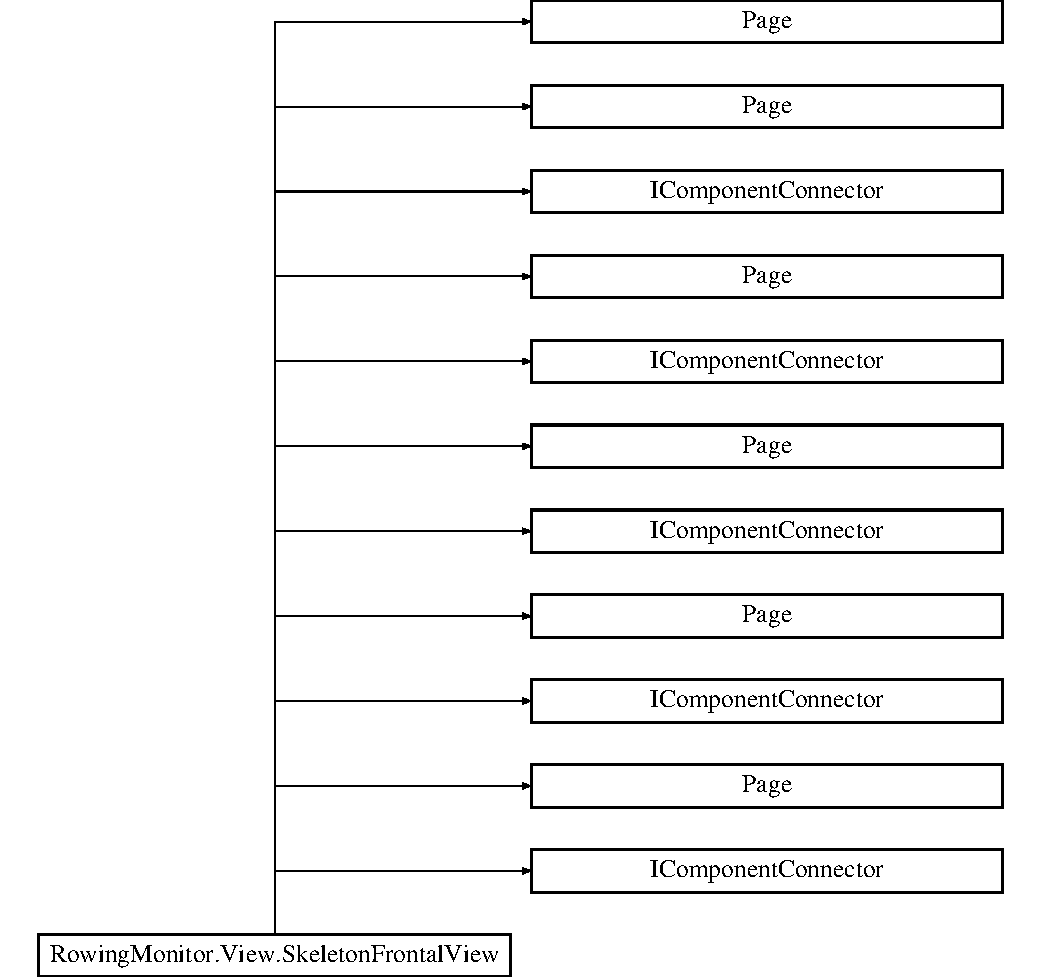
\includegraphics[height=12.000000cm]{class_rowing_monitor_1_1_view_1_1_skeleton_frontal_view}
\end{center}
\end{figure}
\subsection*{Public Member Functions}
\begin{DoxyCompactItemize}
\item 
void \hyperlink{class_rowing_monitor_1_1_view_1_1_skeleton_frontal_view_a47e693425fedb725291469b158ff9625}{Initialize\+Component} ()
\begin{DoxyCompactList}\small\item\em Initialize\+Component \end{DoxyCompactList}\item 
void \hyperlink{class_rowing_monitor_1_1_view_1_1_skeleton_frontal_view_a47e693425fedb725291469b158ff9625}{Initialize\+Component} ()
\begin{DoxyCompactList}\small\item\em Initialize\+Component \end{DoxyCompactList}\item 
void \hyperlink{class_rowing_monitor_1_1_view_1_1_skeleton_frontal_view_a47e693425fedb725291469b158ff9625}{Initialize\+Component} ()
\begin{DoxyCompactList}\small\item\em Initialize\+Component \end{DoxyCompactList}\item 
void \hyperlink{class_rowing_monitor_1_1_view_1_1_skeleton_frontal_view_a47e693425fedb725291469b158ff9625}{Initialize\+Component} ()
\begin{DoxyCompactList}\small\item\em Initialize\+Component \end{DoxyCompactList}\item 
void \hyperlink{class_rowing_monitor_1_1_view_1_1_skeleton_frontal_view_a47e693425fedb725291469b158ff9625}{Initialize\+Component} ()
\begin{DoxyCompactList}\small\item\em Initialize\+Component \end{DoxyCompactList}\item 
\hyperlink{class_rowing_monitor_1_1_view_1_1_skeleton_frontal_view_a7ebe4cc1a0aa4d317d2f15b99ebada40}{Skeleton\+Frontal\+View} ()
\end{DoxyCompactItemize}


\subsection{Detailed Description}
\hyperlink{class_rowing_monitor_1_1_view_1_1_skeleton_frontal_view}{Skeleton\+Frontal\+View} 

Interaktionslogik für Skeleton\+Frontal\+View.\+xaml 

\subsection{Constructor \& Destructor Documentation}
\mbox{\Hypertarget{class_rowing_monitor_1_1_view_1_1_skeleton_frontal_view_a7ebe4cc1a0aa4d317d2f15b99ebada40}\label{class_rowing_monitor_1_1_view_1_1_skeleton_frontal_view_a7ebe4cc1a0aa4d317d2f15b99ebada40}} 
\index{Rowing\+Monitor\+::\+View\+::\+Skeleton\+Frontal\+View@{Rowing\+Monitor\+::\+View\+::\+Skeleton\+Frontal\+View}!Skeleton\+Frontal\+View@{Skeleton\+Frontal\+View}}
\index{Skeleton\+Frontal\+View@{Skeleton\+Frontal\+View}!Rowing\+Monitor\+::\+View\+::\+Skeleton\+Frontal\+View@{Rowing\+Monitor\+::\+View\+::\+Skeleton\+Frontal\+View}}
\subsubsection{\texorpdfstring{Skeleton\+Frontal\+View()}{SkeletonFrontalView()}}
{\footnotesize\ttfamily Rowing\+Monitor.\+View.\+Skeleton\+Frontal\+View.\+Skeleton\+Frontal\+View (\begin{DoxyParamCaption}{ }\end{DoxyParamCaption})}



\subsection{Member Function Documentation}
\mbox{\Hypertarget{class_rowing_monitor_1_1_view_1_1_skeleton_frontal_view_a47e693425fedb725291469b158ff9625}\label{class_rowing_monitor_1_1_view_1_1_skeleton_frontal_view_a47e693425fedb725291469b158ff9625}} 
\index{Rowing\+Monitor\+::\+View\+::\+Skeleton\+Frontal\+View@{Rowing\+Monitor\+::\+View\+::\+Skeleton\+Frontal\+View}!Initialize\+Component@{Initialize\+Component}}
\index{Initialize\+Component@{Initialize\+Component}!Rowing\+Monitor\+::\+View\+::\+Skeleton\+Frontal\+View@{Rowing\+Monitor\+::\+View\+::\+Skeleton\+Frontal\+View}}
\subsubsection{\texorpdfstring{Initialize\+Component()}{InitializeComponent()}\hspace{0.1cm}{\footnotesize\ttfamily [1/5]}}
{\footnotesize\ttfamily void Rowing\+Monitor.\+View.\+Skeleton\+Frontal\+View.\+Initialize\+Component (\begin{DoxyParamCaption}{ }\end{DoxyParamCaption})}



Initialize\+Component 

\mbox{\Hypertarget{class_rowing_monitor_1_1_view_1_1_skeleton_frontal_view_a47e693425fedb725291469b158ff9625}\label{class_rowing_monitor_1_1_view_1_1_skeleton_frontal_view_a47e693425fedb725291469b158ff9625}} 
\index{Rowing\+Monitor\+::\+View\+::\+Skeleton\+Frontal\+View@{Rowing\+Monitor\+::\+View\+::\+Skeleton\+Frontal\+View}!Initialize\+Component@{Initialize\+Component}}
\index{Initialize\+Component@{Initialize\+Component}!Rowing\+Monitor\+::\+View\+::\+Skeleton\+Frontal\+View@{Rowing\+Monitor\+::\+View\+::\+Skeleton\+Frontal\+View}}
\subsubsection{\texorpdfstring{Initialize\+Component()}{InitializeComponent()}\hspace{0.1cm}{\footnotesize\ttfamily [2/5]}}
{\footnotesize\ttfamily void Rowing\+Monitor.\+View.\+Skeleton\+Frontal\+View.\+Initialize\+Component (\begin{DoxyParamCaption}{ }\end{DoxyParamCaption})}



Initialize\+Component 

\mbox{\Hypertarget{class_rowing_monitor_1_1_view_1_1_skeleton_frontal_view_a47e693425fedb725291469b158ff9625}\label{class_rowing_monitor_1_1_view_1_1_skeleton_frontal_view_a47e693425fedb725291469b158ff9625}} 
\index{Rowing\+Monitor\+::\+View\+::\+Skeleton\+Frontal\+View@{Rowing\+Monitor\+::\+View\+::\+Skeleton\+Frontal\+View}!Initialize\+Component@{Initialize\+Component}}
\index{Initialize\+Component@{Initialize\+Component}!Rowing\+Monitor\+::\+View\+::\+Skeleton\+Frontal\+View@{Rowing\+Monitor\+::\+View\+::\+Skeleton\+Frontal\+View}}
\subsubsection{\texorpdfstring{Initialize\+Component()}{InitializeComponent()}\hspace{0.1cm}{\footnotesize\ttfamily [3/5]}}
{\footnotesize\ttfamily void Rowing\+Monitor.\+View.\+Skeleton\+Frontal\+View.\+Initialize\+Component (\begin{DoxyParamCaption}{ }\end{DoxyParamCaption})}



Initialize\+Component 

\mbox{\Hypertarget{class_rowing_monitor_1_1_view_1_1_skeleton_frontal_view_a47e693425fedb725291469b158ff9625}\label{class_rowing_monitor_1_1_view_1_1_skeleton_frontal_view_a47e693425fedb725291469b158ff9625}} 
\index{Rowing\+Monitor\+::\+View\+::\+Skeleton\+Frontal\+View@{Rowing\+Monitor\+::\+View\+::\+Skeleton\+Frontal\+View}!Initialize\+Component@{Initialize\+Component}}
\index{Initialize\+Component@{Initialize\+Component}!Rowing\+Monitor\+::\+View\+::\+Skeleton\+Frontal\+View@{Rowing\+Monitor\+::\+View\+::\+Skeleton\+Frontal\+View}}
\subsubsection{\texorpdfstring{Initialize\+Component()}{InitializeComponent()}\hspace{0.1cm}{\footnotesize\ttfamily [4/5]}}
{\footnotesize\ttfamily void Rowing\+Monitor.\+View.\+Skeleton\+Frontal\+View.\+Initialize\+Component (\begin{DoxyParamCaption}{ }\end{DoxyParamCaption})}



Initialize\+Component 

\mbox{\Hypertarget{class_rowing_monitor_1_1_view_1_1_skeleton_frontal_view_a47e693425fedb725291469b158ff9625}\label{class_rowing_monitor_1_1_view_1_1_skeleton_frontal_view_a47e693425fedb725291469b158ff9625}} 
\index{Rowing\+Monitor\+::\+View\+::\+Skeleton\+Frontal\+View@{Rowing\+Monitor\+::\+View\+::\+Skeleton\+Frontal\+View}!Initialize\+Component@{Initialize\+Component}}
\index{Initialize\+Component@{Initialize\+Component}!Rowing\+Monitor\+::\+View\+::\+Skeleton\+Frontal\+View@{Rowing\+Monitor\+::\+View\+::\+Skeleton\+Frontal\+View}}
\subsubsection{\texorpdfstring{Initialize\+Component()}{InitializeComponent()}\hspace{0.1cm}{\footnotesize\ttfamily [5/5]}}
{\footnotesize\ttfamily void Rowing\+Monitor.\+View.\+Skeleton\+Frontal\+View.\+Initialize\+Component (\begin{DoxyParamCaption}{ }\end{DoxyParamCaption})}



Initialize\+Component 



The documentation for this class was generated from the following files\+:\begin{DoxyCompactItemize}
\item 
obj/\+Debug/\+View/\hyperlink{_skeleton_frontal_view_01-_01_kopieren_8g_8i_8cs}{Skeleton\+Frontal\+View -\/ Kopieren.\+g.\+i.\+cs}\item 
obj/\+Debug/\+View/\hyperlink{_debug_2_view_2_skeleton_frontal_view_8g_8cs}{Skeleton\+Frontal\+View.\+g.\+cs}\item 
obj/\+Debug/\+View/\hyperlink{_debug_2_view_2_skeleton_frontal_view_8g_8i_8cs}{Skeleton\+Frontal\+View.\+g.\+i.\+cs}\item 
View/\hyperlink{_skeleton_frontal_view_8xaml_8cs}{Skeleton\+Frontal\+View.\+xaml.\+cs}\end{DoxyCompactItemize}

\hypertarget{class_rowing_monitor_1_1_view_model_1_1_skeleton_frontal_view_model}{}\section{Rowing\+Monitor.\+View\+Model.\+Skeleton\+Frontal\+View\+Model Class Reference}
\label{class_rowing_monitor_1_1_view_model_1_1_skeleton_frontal_view_model}\index{Rowing\+Monitor.\+View\+Model.\+Skeleton\+Frontal\+View\+Model@{Rowing\+Monitor.\+View\+Model.\+Skeleton\+Frontal\+View\+Model}}
Inheritance diagram for Rowing\+Monitor.\+View\+Model.\+Skeleton\+Frontal\+View\+Model\+:\begin{figure}[H]
\begin{center}
\leavevmode
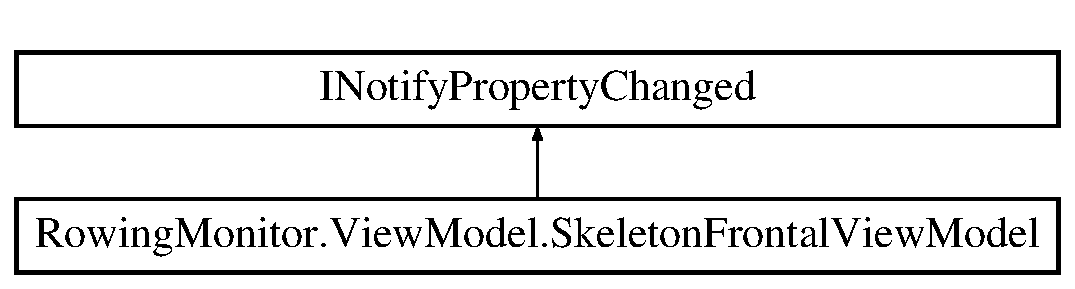
\includegraphics[height=2.000000cm]{class_rowing_monitor_1_1_view_model_1_1_skeleton_frontal_view_model}
\end{center}
\end{figure}
\subsection*{Public Member Functions}
\begin{DoxyCompactItemize}
\item 
\hyperlink{class_rowing_monitor_1_1_view_model_1_1_skeleton_frontal_view_model_a44e3840c22cac26b53fc49f5fa590e7e}{Skeleton\+Frontal\+View\+Model} ()
\item 
void \hyperlink{class_rowing_monitor_1_1_view_model_1_1_skeleton_frontal_view_model_a3b92b388570f66ea804bf228560e0406}{Render} ()
\item 
void \hyperlink{class_rowing_monitor_1_1_view_model_1_1_skeleton_frontal_view_model_a4e8bdb2b5d7464ee464fa35a540a7f9c}{Update\+Skeleton\+Image} (Drawing\+Image skeleton\+Image\+Source)
\item 
void \hyperlink{class_rowing_monitor_1_1_view_model_1_1_skeleton_frontal_view_model_a069c37a99bcce8ffa762892987886f19}{Update\+Color\+Image} (Image\+Source color\+Image\+Source)
\end{DoxyCompactItemize}
\subsection*{Properties}
\begin{DoxyCompactItemize}
\item 
Image\+Source \hyperlink{class_rowing_monitor_1_1_view_model_1_1_skeleton_frontal_view_model_a91b53739cf7c3904497a1d9a34fd6962}{Color\+Image\+Source}\hspace{0.3cm}{\ttfamily  \mbox{[}get, set\mbox{]}}
\item 
Image\+Source \hyperlink{class_rowing_monitor_1_1_view_model_1_1_skeleton_frontal_view_model_a2ab711486ceab54b30c19cc8a349e3f8}{Skeleton\+Image\+Source}\hspace{0.3cm}{\ttfamily  \mbox{[}get, set\mbox{]}}
\end{DoxyCompactItemize}
\subsection*{Events}
\begin{DoxyCompactItemize}
\item 
Property\+Changed\+Event\+Handler \hyperlink{class_rowing_monitor_1_1_view_model_1_1_skeleton_frontal_view_model_a0eab183b09804fc0b512bfaf6ac9ab9c}{Property\+Changed}
\end{DoxyCompactItemize}


\subsection{Constructor \& Destructor Documentation}
\mbox{\Hypertarget{class_rowing_monitor_1_1_view_model_1_1_skeleton_frontal_view_model_a44e3840c22cac26b53fc49f5fa590e7e}\label{class_rowing_monitor_1_1_view_model_1_1_skeleton_frontal_view_model_a44e3840c22cac26b53fc49f5fa590e7e}} 
\index{Rowing\+Monitor\+::\+View\+Model\+::\+Skeleton\+Frontal\+View\+Model@{Rowing\+Monitor\+::\+View\+Model\+::\+Skeleton\+Frontal\+View\+Model}!Skeleton\+Frontal\+View\+Model@{Skeleton\+Frontal\+View\+Model}}
\index{Skeleton\+Frontal\+View\+Model@{Skeleton\+Frontal\+View\+Model}!Rowing\+Monitor\+::\+View\+Model\+::\+Skeleton\+Frontal\+View\+Model@{Rowing\+Monitor\+::\+View\+Model\+::\+Skeleton\+Frontal\+View\+Model}}
\subsubsection{\texorpdfstring{Skeleton\+Frontal\+View\+Model()}{SkeletonFrontalViewModel()}}
{\footnotesize\ttfamily Rowing\+Monitor.\+View\+Model.\+Skeleton\+Frontal\+View\+Model.\+Skeleton\+Frontal\+View\+Model (\begin{DoxyParamCaption}{ }\end{DoxyParamCaption})}



\subsection{Member Function Documentation}
\mbox{\Hypertarget{class_rowing_monitor_1_1_view_model_1_1_skeleton_frontal_view_model_a3b92b388570f66ea804bf228560e0406}\label{class_rowing_monitor_1_1_view_model_1_1_skeleton_frontal_view_model_a3b92b388570f66ea804bf228560e0406}} 
\index{Rowing\+Monitor\+::\+View\+Model\+::\+Skeleton\+Frontal\+View\+Model@{Rowing\+Monitor\+::\+View\+Model\+::\+Skeleton\+Frontal\+View\+Model}!Render@{Render}}
\index{Render@{Render}!Rowing\+Monitor\+::\+View\+Model\+::\+Skeleton\+Frontal\+View\+Model@{Rowing\+Monitor\+::\+View\+Model\+::\+Skeleton\+Frontal\+View\+Model}}
\subsubsection{\texorpdfstring{Render()}{Render()}}
{\footnotesize\ttfamily void Rowing\+Monitor.\+View\+Model.\+Skeleton\+Frontal\+View\+Model.\+Render (\begin{DoxyParamCaption}{ }\end{DoxyParamCaption})}

\mbox{\Hypertarget{class_rowing_monitor_1_1_view_model_1_1_skeleton_frontal_view_model_a069c37a99bcce8ffa762892987886f19}\label{class_rowing_monitor_1_1_view_model_1_1_skeleton_frontal_view_model_a069c37a99bcce8ffa762892987886f19}} 
\index{Rowing\+Monitor\+::\+View\+Model\+::\+Skeleton\+Frontal\+View\+Model@{Rowing\+Monitor\+::\+View\+Model\+::\+Skeleton\+Frontal\+View\+Model}!Update\+Color\+Image@{Update\+Color\+Image}}
\index{Update\+Color\+Image@{Update\+Color\+Image}!Rowing\+Monitor\+::\+View\+Model\+::\+Skeleton\+Frontal\+View\+Model@{Rowing\+Monitor\+::\+View\+Model\+::\+Skeleton\+Frontal\+View\+Model}}
\subsubsection{\texorpdfstring{Update\+Color\+Image()}{UpdateColorImage()}}
{\footnotesize\ttfamily void Rowing\+Monitor.\+View\+Model.\+Skeleton\+Frontal\+View\+Model.\+Update\+Color\+Image (\begin{DoxyParamCaption}\item[{Image\+Source}]{color\+Image\+Source }\end{DoxyParamCaption})}

\mbox{\Hypertarget{class_rowing_monitor_1_1_view_model_1_1_skeleton_frontal_view_model_a4e8bdb2b5d7464ee464fa35a540a7f9c}\label{class_rowing_monitor_1_1_view_model_1_1_skeleton_frontal_view_model_a4e8bdb2b5d7464ee464fa35a540a7f9c}} 
\index{Rowing\+Monitor\+::\+View\+Model\+::\+Skeleton\+Frontal\+View\+Model@{Rowing\+Monitor\+::\+View\+Model\+::\+Skeleton\+Frontal\+View\+Model}!Update\+Skeleton\+Image@{Update\+Skeleton\+Image}}
\index{Update\+Skeleton\+Image@{Update\+Skeleton\+Image}!Rowing\+Monitor\+::\+View\+Model\+::\+Skeleton\+Frontal\+View\+Model@{Rowing\+Monitor\+::\+View\+Model\+::\+Skeleton\+Frontal\+View\+Model}}
\subsubsection{\texorpdfstring{Update\+Skeleton\+Image()}{UpdateSkeletonImage()}}
{\footnotesize\ttfamily void Rowing\+Monitor.\+View\+Model.\+Skeleton\+Frontal\+View\+Model.\+Update\+Skeleton\+Image (\begin{DoxyParamCaption}\item[{Drawing\+Image}]{skeleton\+Image\+Source }\end{DoxyParamCaption})}



\subsection{Property Documentation}
\mbox{\Hypertarget{class_rowing_monitor_1_1_view_model_1_1_skeleton_frontal_view_model_a91b53739cf7c3904497a1d9a34fd6962}\label{class_rowing_monitor_1_1_view_model_1_1_skeleton_frontal_view_model_a91b53739cf7c3904497a1d9a34fd6962}} 
\index{Rowing\+Monitor\+::\+View\+Model\+::\+Skeleton\+Frontal\+View\+Model@{Rowing\+Monitor\+::\+View\+Model\+::\+Skeleton\+Frontal\+View\+Model}!Color\+Image\+Source@{Color\+Image\+Source}}
\index{Color\+Image\+Source@{Color\+Image\+Source}!Rowing\+Monitor\+::\+View\+Model\+::\+Skeleton\+Frontal\+View\+Model@{Rowing\+Monitor\+::\+View\+Model\+::\+Skeleton\+Frontal\+View\+Model}}
\subsubsection{\texorpdfstring{Color\+Image\+Source}{ColorImageSource}}
{\footnotesize\ttfamily Image\+Source Rowing\+Monitor.\+View\+Model.\+Skeleton\+Frontal\+View\+Model.\+Color\+Image\+Source\hspace{0.3cm}{\ttfamily [get]}, {\ttfamily [set]}}

\mbox{\Hypertarget{class_rowing_monitor_1_1_view_model_1_1_skeleton_frontal_view_model_a2ab711486ceab54b30c19cc8a349e3f8}\label{class_rowing_monitor_1_1_view_model_1_1_skeleton_frontal_view_model_a2ab711486ceab54b30c19cc8a349e3f8}} 
\index{Rowing\+Monitor\+::\+View\+Model\+::\+Skeleton\+Frontal\+View\+Model@{Rowing\+Monitor\+::\+View\+Model\+::\+Skeleton\+Frontal\+View\+Model}!Skeleton\+Image\+Source@{Skeleton\+Image\+Source}}
\index{Skeleton\+Image\+Source@{Skeleton\+Image\+Source}!Rowing\+Monitor\+::\+View\+Model\+::\+Skeleton\+Frontal\+View\+Model@{Rowing\+Monitor\+::\+View\+Model\+::\+Skeleton\+Frontal\+View\+Model}}
\subsubsection{\texorpdfstring{Skeleton\+Image\+Source}{SkeletonImageSource}}
{\footnotesize\ttfamily Image\+Source Rowing\+Monitor.\+View\+Model.\+Skeleton\+Frontal\+View\+Model.\+Skeleton\+Image\+Source\hspace{0.3cm}{\ttfamily [get]}, {\ttfamily [set]}}



\subsection{Event Documentation}
\mbox{\Hypertarget{class_rowing_monitor_1_1_view_model_1_1_skeleton_frontal_view_model_a0eab183b09804fc0b512bfaf6ac9ab9c}\label{class_rowing_monitor_1_1_view_model_1_1_skeleton_frontal_view_model_a0eab183b09804fc0b512bfaf6ac9ab9c}} 
\index{Rowing\+Monitor\+::\+View\+Model\+::\+Skeleton\+Frontal\+View\+Model@{Rowing\+Monitor\+::\+View\+Model\+::\+Skeleton\+Frontal\+View\+Model}!Property\+Changed@{Property\+Changed}}
\index{Property\+Changed@{Property\+Changed}!Rowing\+Monitor\+::\+View\+Model\+::\+Skeleton\+Frontal\+View\+Model@{Rowing\+Monitor\+::\+View\+Model\+::\+Skeleton\+Frontal\+View\+Model}}
\subsubsection{\texorpdfstring{Property\+Changed}{PropertyChanged}}
{\footnotesize\ttfamily Property\+Changed\+Event\+Handler Rowing\+Monitor.\+View\+Model.\+Skeleton\+Frontal\+View\+Model.\+Property\+Changed}



The documentation for this class was generated from the following file\+:\begin{DoxyCompactItemize}
\item 
View\+Model/\hyperlink{_skeleton_frontal_view_model_8cs}{Skeleton\+Frontal\+View\+Model.\+cs}\end{DoxyCompactItemize}

\hypertarget{class_rowing_monitor_1_1_model_1_1_pipeline_1_1_skeleton_side_display}{}\section{Rowing\+Monitor.\+Model.\+Pipeline.\+Skeleton\+Side\+Display Class Reference}
\label{class_rowing_monitor_1_1_model_1_1_pipeline_1_1_skeleton_side_display}\index{Rowing\+Monitor.\+Model.\+Pipeline.\+Skeleton\+Side\+Display@{Rowing\+Monitor.\+Model.\+Pipeline.\+Skeleton\+Side\+Display}}
\subsection*{Public Member Functions}
\begin{DoxyCompactItemize}
\item 
\hyperlink{class_rowing_monitor_1_1_model_1_1_pipeline_1_1_skeleton_side_display_aa9cea6100e45eb5dd9ce60141287659d}{Skeleton\+Side\+Display} ()
\item 
void \hyperlink{class_rowing_monitor_1_1_model_1_1_pipeline_1_1_skeleton_side_display_a5957c0188fc2ceabae1e20f0d8c2c057}{Render} ()
\item 
virtual void \hyperlink{class_rowing_monitor_1_1_model_1_1_pipeline_1_1_skeleton_side_display_a3bd1bbfaa2c32be913414b1e4cd8a32d}{Update\+Skeleton} (I\+Read\+Only\+Dictionary$<$ Joint\+Type, Joint $>$ joints)
\begin{DoxyCompactList}\small\item\em Updates the view with new data. \end{DoxyCompactList}\end{DoxyCompactItemize}
\subsection*{Protected Member Functions}
\begin{DoxyCompactItemize}
\item 
void \hyperlink{class_rowing_monitor_1_1_model_1_1_pipeline_1_1_skeleton_side_display_af2a9cdb39da2e18683de666a255e5015}{Draw\+Body} (I\+Read\+Only\+Dictionary$<$ Joint\+Type, Joint $>$ joints, I\+Dictionary$<$ Joint\+Type, Point $>$ joint\+Points, Drawing\+Context drawing\+Context)
\begin{DoxyCompactList}\small\item\em Draws a body \end{DoxyCompactList}\end{DoxyCompactItemize}
\subsection*{Protected Attributes}
\begin{DoxyCompactItemize}
\item 
const float \hyperlink{class_rowing_monitor_1_1_model_1_1_pipeline_1_1_skeleton_side_display_a1d54abd0be96b596c42bdf768df42b5d}{Inferred\+Z\+Position\+Clamp} = 0.\+1f
\begin{DoxyCompactList}\small\item\em Constant for clamping Z values of camera space points from being negative \end{DoxyCompactList}\end{DoxyCompactItemize}
\subsection*{Properties}
\begin{DoxyCompactItemize}
\item 
Action\+Block$<$ \hyperlink{struct_rowing_monitor_1_1_model_1_1_util_1_1_joint_data}{Joint\+Data} $>$ \hyperlink{class_rowing_monitor_1_1_model_1_1_pipeline_1_1_skeleton_side_display_a6b8216c1f921a661999c1f9e419a70b1}{Skeleton\+Block}\hspace{0.3cm}{\ttfamily  \mbox{[}get, set\mbox{]}}
\item 
\hyperlink{class_rowing_monitor_1_1_view_1_1_skeleton_side_view}{Skeleton\+Side\+View} \hyperlink{class_rowing_monitor_1_1_model_1_1_pipeline_1_1_skeleton_side_display_ad3a2bc2fd40be1be27bc7a6e081e4993}{View}\hspace{0.3cm}{\ttfamily  \mbox{[}get, set\mbox{]}}
\item 
float \hyperlink{class_rowing_monitor_1_1_model_1_1_pipeline_1_1_skeleton_side_display_a0d3755d630c80878a72d5f7ef598983f}{Area\+Width}\hspace{0.3cm}{\ttfamily  \mbox{[}get, set\mbox{]}}
\item 
bool \hyperlink{class_rowing_monitor_1_1_model_1_1_pipeline_1_1_skeleton_side_display_a09ff87b46af582c486dab5ed3bab5aec}{Show\+Hand\+Trajectory}\hspace{0.3cm}{\ttfamily  \mbox{[}get, set\mbox{]}}
\item 
bool \hyperlink{class_rowing_monitor_1_1_model_1_1_pipeline_1_1_skeleton_side_display_a0d609dc0262350737aaf01b5e4588076}{Show\+Body\+C\+O\+M\+Trajectory}\hspace{0.3cm}{\ttfamily  \mbox{[}get, set\mbox{]}}
\item 
bool \hyperlink{class_rowing_monitor_1_1_model_1_1_pipeline_1_1_skeleton_side_display_a0c914a7629c874ae9b23137754938959}{Show\+Foot\+Hip\+Connection}\hspace{0.3cm}{\ttfamily  \mbox{[}get, set\mbox{]}}
\item 
bool \hyperlink{class_rowing_monitor_1_1_model_1_1_pipeline_1_1_skeleton_side_display_a9e69f5b1f04aea33ec07b36236989f58}{Show\+Knee\+Trajectory}\hspace{0.3cm}{\ttfamily  \mbox{[}get, set\mbox{]}}
\end{DoxyCompactItemize}


\subsection{Constructor \& Destructor Documentation}
\mbox{\Hypertarget{class_rowing_monitor_1_1_model_1_1_pipeline_1_1_skeleton_side_display_aa9cea6100e45eb5dd9ce60141287659d}\label{class_rowing_monitor_1_1_model_1_1_pipeline_1_1_skeleton_side_display_aa9cea6100e45eb5dd9ce60141287659d}} 
\index{Rowing\+Monitor\+::\+Model\+::\+Pipeline\+::\+Skeleton\+Side\+Display@{Rowing\+Monitor\+::\+Model\+::\+Pipeline\+::\+Skeleton\+Side\+Display}!Skeleton\+Side\+Display@{Skeleton\+Side\+Display}}
\index{Skeleton\+Side\+Display@{Skeleton\+Side\+Display}!Rowing\+Monitor\+::\+Model\+::\+Pipeline\+::\+Skeleton\+Side\+Display@{Rowing\+Monitor\+::\+Model\+::\+Pipeline\+::\+Skeleton\+Side\+Display}}
\subsubsection{\texorpdfstring{Skeleton\+Side\+Display()}{SkeletonSideDisplay()}}
{\footnotesize\ttfamily Rowing\+Monitor.\+Model.\+Pipeline.\+Skeleton\+Side\+Display.\+Skeleton\+Side\+Display (\begin{DoxyParamCaption}{ }\end{DoxyParamCaption})}



\subsection{Member Function Documentation}
\mbox{\Hypertarget{class_rowing_monitor_1_1_model_1_1_pipeline_1_1_skeleton_side_display_af2a9cdb39da2e18683de666a255e5015}\label{class_rowing_monitor_1_1_model_1_1_pipeline_1_1_skeleton_side_display_af2a9cdb39da2e18683de666a255e5015}} 
\index{Rowing\+Monitor\+::\+Model\+::\+Pipeline\+::\+Skeleton\+Side\+Display@{Rowing\+Monitor\+::\+Model\+::\+Pipeline\+::\+Skeleton\+Side\+Display}!Draw\+Body@{Draw\+Body}}
\index{Draw\+Body@{Draw\+Body}!Rowing\+Monitor\+::\+Model\+::\+Pipeline\+::\+Skeleton\+Side\+Display@{Rowing\+Monitor\+::\+Model\+::\+Pipeline\+::\+Skeleton\+Side\+Display}}
\subsubsection{\texorpdfstring{Draw\+Body()}{DrawBody()}}
{\footnotesize\ttfamily void Rowing\+Monitor.\+Model.\+Pipeline.\+Skeleton\+Side\+Display.\+Draw\+Body (\begin{DoxyParamCaption}\item[{I\+Read\+Only\+Dictionary$<$ Joint\+Type, Joint $>$}]{joints,  }\item[{I\+Dictionary$<$ Joint\+Type, Point $>$}]{joint\+Points,  }\item[{Drawing\+Context}]{drawing\+Context }\end{DoxyParamCaption})\hspace{0.3cm}{\ttfamily [protected]}}



Draws a body 


\begin{DoxyParams}{Parameters}
{\em joints} & joints to draw\\
\hline
{\em joint\+Points} & translated positions of joints to draw\\
\hline
{\em drawing\+Context} & drawing context to draw to\\
\hline
\end{DoxyParams}
\mbox{\Hypertarget{class_rowing_monitor_1_1_model_1_1_pipeline_1_1_skeleton_side_display_a5957c0188fc2ceabae1e20f0d8c2c057}\label{class_rowing_monitor_1_1_model_1_1_pipeline_1_1_skeleton_side_display_a5957c0188fc2ceabae1e20f0d8c2c057}} 
\index{Rowing\+Monitor\+::\+Model\+::\+Pipeline\+::\+Skeleton\+Side\+Display@{Rowing\+Monitor\+::\+Model\+::\+Pipeline\+::\+Skeleton\+Side\+Display}!Render@{Render}}
\index{Render@{Render}!Rowing\+Monitor\+::\+Model\+::\+Pipeline\+::\+Skeleton\+Side\+Display@{Rowing\+Monitor\+::\+Model\+::\+Pipeline\+::\+Skeleton\+Side\+Display}}
\subsubsection{\texorpdfstring{Render()}{Render()}}
{\footnotesize\ttfamily void Rowing\+Monitor.\+Model.\+Pipeline.\+Skeleton\+Side\+Display.\+Render (\begin{DoxyParamCaption}{ }\end{DoxyParamCaption})}

\mbox{\Hypertarget{class_rowing_monitor_1_1_model_1_1_pipeline_1_1_skeleton_side_display_a3bd1bbfaa2c32be913414b1e4cd8a32d}\label{class_rowing_monitor_1_1_model_1_1_pipeline_1_1_skeleton_side_display_a3bd1bbfaa2c32be913414b1e4cd8a32d}} 
\index{Rowing\+Monitor\+::\+Model\+::\+Pipeline\+::\+Skeleton\+Side\+Display@{Rowing\+Monitor\+::\+Model\+::\+Pipeline\+::\+Skeleton\+Side\+Display}!Update\+Skeleton@{Update\+Skeleton}}
\index{Update\+Skeleton@{Update\+Skeleton}!Rowing\+Monitor\+::\+Model\+::\+Pipeline\+::\+Skeleton\+Side\+Display@{Rowing\+Monitor\+::\+Model\+::\+Pipeline\+::\+Skeleton\+Side\+Display}}
\subsubsection{\texorpdfstring{Update\+Skeleton()}{UpdateSkeleton()}}
{\footnotesize\ttfamily virtual void Rowing\+Monitor.\+Model.\+Pipeline.\+Skeleton\+Side\+Display.\+Update\+Skeleton (\begin{DoxyParamCaption}\item[{I\+Read\+Only\+Dictionary$<$ Joint\+Type, Joint $>$}]{joints }\end{DoxyParamCaption})\hspace{0.3cm}{\ttfamily [virtual]}}



Updates the view with new data. 



\subsection{Member Data Documentation}
\mbox{\Hypertarget{class_rowing_monitor_1_1_model_1_1_pipeline_1_1_skeleton_side_display_a1d54abd0be96b596c42bdf768df42b5d}\label{class_rowing_monitor_1_1_model_1_1_pipeline_1_1_skeleton_side_display_a1d54abd0be96b596c42bdf768df42b5d}} 
\index{Rowing\+Monitor\+::\+Model\+::\+Pipeline\+::\+Skeleton\+Side\+Display@{Rowing\+Monitor\+::\+Model\+::\+Pipeline\+::\+Skeleton\+Side\+Display}!Inferred\+Z\+Position\+Clamp@{Inferred\+Z\+Position\+Clamp}}
\index{Inferred\+Z\+Position\+Clamp@{Inferred\+Z\+Position\+Clamp}!Rowing\+Monitor\+::\+Model\+::\+Pipeline\+::\+Skeleton\+Side\+Display@{Rowing\+Monitor\+::\+Model\+::\+Pipeline\+::\+Skeleton\+Side\+Display}}
\subsubsection{\texorpdfstring{Inferred\+Z\+Position\+Clamp}{InferredZPositionClamp}}
{\footnotesize\ttfamily const float Rowing\+Monitor.\+Model.\+Pipeline.\+Skeleton\+Side\+Display.\+Inferred\+Z\+Position\+Clamp = 0.\+1f\hspace{0.3cm}{\ttfamily [protected]}}



Constant for clamping Z values of camera space points from being negative 



\subsection{Property Documentation}
\mbox{\Hypertarget{class_rowing_monitor_1_1_model_1_1_pipeline_1_1_skeleton_side_display_a0d3755d630c80878a72d5f7ef598983f}\label{class_rowing_monitor_1_1_model_1_1_pipeline_1_1_skeleton_side_display_a0d3755d630c80878a72d5f7ef598983f}} 
\index{Rowing\+Monitor\+::\+Model\+::\+Pipeline\+::\+Skeleton\+Side\+Display@{Rowing\+Monitor\+::\+Model\+::\+Pipeline\+::\+Skeleton\+Side\+Display}!Area\+Width@{Area\+Width}}
\index{Area\+Width@{Area\+Width}!Rowing\+Monitor\+::\+Model\+::\+Pipeline\+::\+Skeleton\+Side\+Display@{Rowing\+Monitor\+::\+Model\+::\+Pipeline\+::\+Skeleton\+Side\+Display}}
\subsubsection{\texorpdfstring{Area\+Width}{AreaWidth}}
{\footnotesize\ttfamily float Rowing\+Monitor.\+Model.\+Pipeline.\+Skeleton\+Side\+Display.\+Area\+Width\hspace{0.3cm}{\ttfamily [get]}, {\ttfamily [set]}}

\mbox{\Hypertarget{class_rowing_monitor_1_1_model_1_1_pipeline_1_1_skeleton_side_display_a0d609dc0262350737aaf01b5e4588076}\label{class_rowing_monitor_1_1_model_1_1_pipeline_1_1_skeleton_side_display_a0d609dc0262350737aaf01b5e4588076}} 
\index{Rowing\+Monitor\+::\+Model\+::\+Pipeline\+::\+Skeleton\+Side\+Display@{Rowing\+Monitor\+::\+Model\+::\+Pipeline\+::\+Skeleton\+Side\+Display}!Show\+Body\+C\+O\+M\+Trajectory@{Show\+Body\+C\+O\+M\+Trajectory}}
\index{Show\+Body\+C\+O\+M\+Trajectory@{Show\+Body\+C\+O\+M\+Trajectory}!Rowing\+Monitor\+::\+Model\+::\+Pipeline\+::\+Skeleton\+Side\+Display@{Rowing\+Monitor\+::\+Model\+::\+Pipeline\+::\+Skeleton\+Side\+Display}}
\subsubsection{\texorpdfstring{Show\+Body\+C\+O\+M\+Trajectory}{ShowBodyCOMTrajectory}}
{\footnotesize\ttfamily bool Rowing\+Monitor.\+Model.\+Pipeline.\+Skeleton\+Side\+Display.\+Show\+Body\+C\+O\+M\+Trajectory\hspace{0.3cm}{\ttfamily [get]}, {\ttfamily [set]}}

\mbox{\Hypertarget{class_rowing_monitor_1_1_model_1_1_pipeline_1_1_skeleton_side_display_a0c914a7629c874ae9b23137754938959}\label{class_rowing_monitor_1_1_model_1_1_pipeline_1_1_skeleton_side_display_a0c914a7629c874ae9b23137754938959}} 
\index{Rowing\+Monitor\+::\+Model\+::\+Pipeline\+::\+Skeleton\+Side\+Display@{Rowing\+Monitor\+::\+Model\+::\+Pipeline\+::\+Skeleton\+Side\+Display}!Show\+Foot\+Hip\+Connection@{Show\+Foot\+Hip\+Connection}}
\index{Show\+Foot\+Hip\+Connection@{Show\+Foot\+Hip\+Connection}!Rowing\+Monitor\+::\+Model\+::\+Pipeline\+::\+Skeleton\+Side\+Display@{Rowing\+Monitor\+::\+Model\+::\+Pipeline\+::\+Skeleton\+Side\+Display}}
\subsubsection{\texorpdfstring{Show\+Foot\+Hip\+Connection}{ShowFootHipConnection}}
{\footnotesize\ttfamily bool Rowing\+Monitor.\+Model.\+Pipeline.\+Skeleton\+Side\+Display.\+Show\+Foot\+Hip\+Connection\hspace{0.3cm}{\ttfamily [get]}, {\ttfamily [set]}}

\mbox{\Hypertarget{class_rowing_monitor_1_1_model_1_1_pipeline_1_1_skeleton_side_display_a09ff87b46af582c486dab5ed3bab5aec}\label{class_rowing_monitor_1_1_model_1_1_pipeline_1_1_skeleton_side_display_a09ff87b46af582c486dab5ed3bab5aec}} 
\index{Rowing\+Monitor\+::\+Model\+::\+Pipeline\+::\+Skeleton\+Side\+Display@{Rowing\+Monitor\+::\+Model\+::\+Pipeline\+::\+Skeleton\+Side\+Display}!Show\+Hand\+Trajectory@{Show\+Hand\+Trajectory}}
\index{Show\+Hand\+Trajectory@{Show\+Hand\+Trajectory}!Rowing\+Monitor\+::\+Model\+::\+Pipeline\+::\+Skeleton\+Side\+Display@{Rowing\+Monitor\+::\+Model\+::\+Pipeline\+::\+Skeleton\+Side\+Display}}
\subsubsection{\texorpdfstring{Show\+Hand\+Trajectory}{ShowHandTrajectory}}
{\footnotesize\ttfamily bool Rowing\+Monitor.\+Model.\+Pipeline.\+Skeleton\+Side\+Display.\+Show\+Hand\+Trajectory\hspace{0.3cm}{\ttfamily [get]}, {\ttfamily [set]}}

\mbox{\Hypertarget{class_rowing_monitor_1_1_model_1_1_pipeline_1_1_skeleton_side_display_a9e69f5b1f04aea33ec07b36236989f58}\label{class_rowing_monitor_1_1_model_1_1_pipeline_1_1_skeleton_side_display_a9e69f5b1f04aea33ec07b36236989f58}} 
\index{Rowing\+Monitor\+::\+Model\+::\+Pipeline\+::\+Skeleton\+Side\+Display@{Rowing\+Monitor\+::\+Model\+::\+Pipeline\+::\+Skeleton\+Side\+Display}!Show\+Knee\+Trajectory@{Show\+Knee\+Trajectory}}
\index{Show\+Knee\+Trajectory@{Show\+Knee\+Trajectory}!Rowing\+Monitor\+::\+Model\+::\+Pipeline\+::\+Skeleton\+Side\+Display@{Rowing\+Monitor\+::\+Model\+::\+Pipeline\+::\+Skeleton\+Side\+Display}}
\subsubsection{\texorpdfstring{Show\+Knee\+Trajectory}{ShowKneeTrajectory}}
{\footnotesize\ttfamily bool Rowing\+Monitor.\+Model.\+Pipeline.\+Skeleton\+Side\+Display.\+Show\+Knee\+Trajectory\hspace{0.3cm}{\ttfamily [get]}, {\ttfamily [set]}}

\mbox{\Hypertarget{class_rowing_monitor_1_1_model_1_1_pipeline_1_1_skeleton_side_display_a6b8216c1f921a661999c1f9e419a70b1}\label{class_rowing_monitor_1_1_model_1_1_pipeline_1_1_skeleton_side_display_a6b8216c1f921a661999c1f9e419a70b1}} 
\index{Rowing\+Monitor\+::\+Model\+::\+Pipeline\+::\+Skeleton\+Side\+Display@{Rowing\+Monitor\+::\+Model\+::\+Pipeline\+::\+Skeleton\+Side\+Display}!Skeleton\+Block@{Skeleton\+Block}}
\index{Skeleton\+Block@{Skeleton\+Block}!Rowing\+Monitor\+::\+Model\+::\+Pipeline\+::\+Skeleton\+Side\+Display@{Rowing\+Monitor\+::\+Model\+::\+Pipeline\+::\+Skeleton\+Side\+Display}}
\subsubsection{\texorpdfstring{Skeleton\+Block}{SkeletonBlock}}
{\footnotesize\ttfamily Action\+Block$<$\hyperlink{struct_rowing_monitor_1_1_model_1_1_util_1_1_joint_data}{Joint\+Data}$>$ Rowing\+Monitor.\+Model.\+Pipeline.\+Skeleton\+Side\+Display.\+Skeleton\+Block\hspace{0.3cm}{\ttfamily [get]}, {\ttfamily [set]}}

\mbox{\Hypertarget{class_rowing_monitor_1_1_model_1_1_pipeline_1_1_skeleton_side_display_ad3a2bc2fd40be1be27bc7a6e081e4993}\label{class_rowing_monitor_1_1_model_1_1_pipeline_1_1_skeleton_side_display_ad3a2bc2fd40be1be27bc7a6e081e4993}} 
\index{Rowing\+Monitor\+::\+Model\+::\+Pipeline\+::\+Skeleton\+Side\+Display@{Rowing\+Monitor\+::\+Model\+::\+Pipeline\+::\+Skeleton\+Side\+Display}!View@{View}}
\index{View@{View}!Rowing\+Monitor\+::\+Model\+::\+Pipeline\+::\+Skeleton\+Side\+Display@{Rowing\+Monitor\+::\+Model\+::\+Pipeline\+::\+Skeleton\+Side\+Display}}
\subsubsection{\texorpdfstring{View}{View}}
{\footnotesize\ttfamily \hyperlink{class_rowing_monitor_1_1_view_1_1_skeleton_side_view}{Skeleton\+Side\+View} Rowing\+Monitor.\+Model.\+Pipeline.\+Skeleton\+Side\+Display.\+View\hspace{0.3cm}{\ttfamily [get]}, {\ttfamily [set]}}



The documentation for this class was generated from the following file\+:\begin{DoxyCompactItemize}
\item 
Model/\+Pipeline/\hyperlink{_skeleton_side_display_8cs}{Skeleton\+Side\+Display.\+cs}\end{DoxyCompactItemize}

\hypertarget{class_rowing_monitor_1_1_view_1_1_skeleton_side_view}{}\section{Rowing\+Monitor.\+View.\+Skeleton\+Side\+View Class Reference}
\label{class_rowing_monitor_1_1_view_1_1_skeleton_side_view}\index{Rowing\+Monitor.\+View.\+Skeleton\+Side\+View@{Rowing\+Monitor.\+View.\+Skeleton\+Side\+View}}


\hyperlink{class_rowing_monitor_1_1_view_1_1_skeleton_side_view}{Skeleton\+Side\+View}  


Inheritance diagram for Rowing\+Monitor.\+View.\+Skeleton\+Side\+View\+:\begin{figure}[H]
\begin{center}
\leavevmode
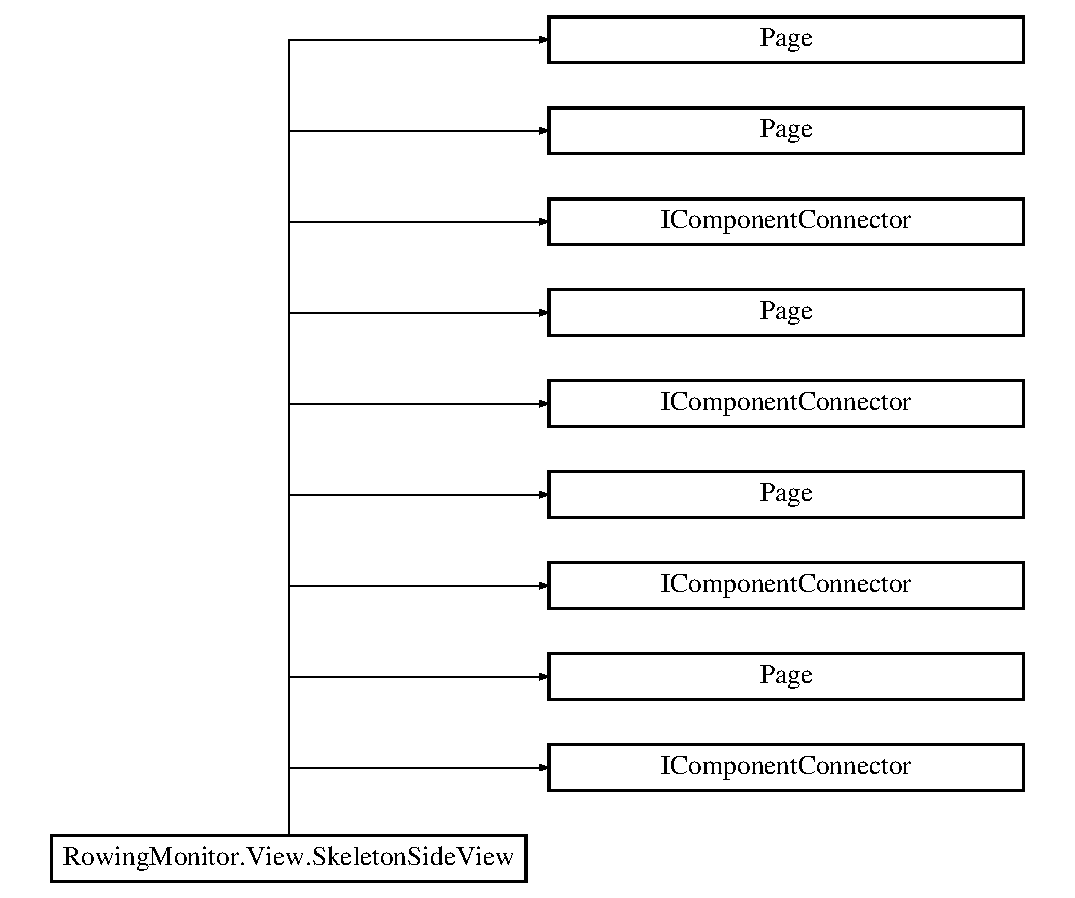
\includegraphics[height=10.000000cm]{class_rowing_monitor_1_1_view_1_1_skeleton_side_view}
\end{center}
\end{figure}
\subsection*{Public Member Functions}
\begin{DoxyCompactItemize}
\item 
void \hyperlink{class_rowing_monitor_1_1_view_1_1_skeleton_side_view_ae823832e7aa40c2585f66c0939c83040}{Initialize\+Component} ()
\begin{DoxyCompactList}\small\item\em Initialize\+Component \end{DoxyCompactList}\item 
void \hyperlink{class_rowing_monitor_1_1_view_1_1_skeleton_side_view_ae823832e7aa40c2585f66c0939c83040}{Initialize\+Component} ()
\begin{DoxyCompactList}\small\item\em Initialize\+Component \end{DoxyCompactList}\item 
void \hyperlink{class_rowing_monitor_1_1_view_1_1_skeleton_side_view_ae823832e7aa40c2585f66c0939c83040}{Initialize\+Component} ()
\begin{DoxyCompactList}\small\item\em Initialize\+Component \end{DoxyCompactList}\item 
void \hyperlink{class_rowing_monitor_1_1_view_1_1_skeleton_side_view_ae823832e7aa40c2585f66c0939c83040}{Initialize\+Component} ()
\begin{DoxyCompactList}\small\item\em Initialize\+Component \end{DoxyCompactList}\item 
\hyperlink{class_rowing_monitor_1_1_view_1_1_skeleton_side_view_ac992a058049b0260d490432660e52650}{Skeleton\+Side\+View} ()
\end{DoxyCompactItemize}


\subsection{Detailed Description}
\hyperlink{class_rowing_monitor_1_1_view_1_1_skeleton_side_view}{Skeleton\+Side\+View} 

Interaktionslogik für Skeleton\+Frontal\+View.\+xaml 

\subsection{Constructor \& Destructor Documentation}
\mbox{\Hypertarget{class_rowing_monitor_1_1_view_1_1_skeleton_side_view_ac992a058049b0260d490432660e52650}\label{class_rowing_monitor_1_1_view_1_1_skeleton_side_view_ac992a058049b0260d490432660e52650}} 
\index{Rowing\+Monitor\+::\+View\+::\+Skeleton\+Side\+View@{Rowing\+Monitor\+::\+View\+::\+Skeleton\+Side\+View}!Skeleton\+Side\+View@{Skeleton\+Side\+View}}
\index{Skeleton\+Side\+View@{Skeleton\+Side\+View}!Rowing\+Monitor\+::\+View\+::\+Skeleton\+Side\+View@{Rowing\+Monitor\+::\+View\+::\+Skeleton\+Side\+View}}
\subsubsection{\texorpdfstring{Skeleton\+Side\+View()}{SkeletonSideView()}}
{\footnotesize\ttfamily Rowing\+Monitor.\+View.\+Skeleton\+Side\+View.\+Skeleton\+Side\+View (\begin{DoxyParamCaption}{ }\end{DoxyParamCaption})}



\subsection{Member Function Documentation}
\mbox{\Hypertarget{class_rowing_monitor_1_1_view_1_1_skeleton_side_view_ae823832e7aa40c2585f66c0939c83040}\label{class_rowing_monitor_1_1_view_1_1_skeleton_side_view_ae823832e7aa40c2585f66c0939c83040}} 
\index{Rowing\+Monitor\+::\+View\+::\+Skeleton\+Side\+View@{Rowing\+Monitor\+::\+View\+::\+Skeleton\+Side\+View}!Initialize\+Component@{Initialize\+Component}}
\index{Initialize\+Component@{Initialize\+Component}!Rowing\+Monitor\+::\+View\+::\+Skeleton\+Side\+View@{Rowing\+Monitor\+::\+View\+::\+Skeleton\+Side\+View}}
\subsubsection{\texorpdfstring{Initialize\+Component()}{InitializeComponent()}\hspace{0.1cm}{\footnotesize\ttfamily [1/4]}}
{\footnotesize\ttfamily void Rowing\+Monitor.\+View.\+Skeleton\+Side\+View.\+Initialize\+Component (\begin{DoxyParamCaption}{ }\end{DoxyParamCaption})}



Initialize\+Component 

\mbox{\Hypertarget{class_rowing_monitor_1_1_view_1_1_skeleton_side_view_ae823832e7aa40c2585f66c0939c83040}\label{class_rowing_monitor_1_1_view_1_1_skeleton_side_view_ae823832e7aa40c2585f66c0939c83040}} 
\index{Rowing\+Monitor\+::\+View\+::\+Skeleton\+Side\+View@{Rowing\+Monitor\+::\+View\+::\+Skeleton\+Side\+View}!Initialize\+Component@{Initialize\+Component}}
\index{Initialize\+Component@{Initialize\+Component}!Rowing\+Monitor\+::\+View\+::\+Skeleton\+Side\+View@{Rowing\+Monitor\+::\+View\+::\+Skeleton\+Side\+View}}
\subsubsection{\texorpdfstring{Initialize\+Component()}{InitializeComponent()}\hspace{0.1cm}{\footnotesize\ttfamily [2/4]}}
{\footnotesize\ttfamily void Rowing\+Monitor.\+View.\+Skeleton\+Side\+View.\+Initialize\+Component (\begin{DoxyParamCaption}{ }\end{DoxyParamCaption})}



Initialize\+Component 

\mbox{\Hypertarget{class_rowing_monitor_1_1_view_1_1_skeleton_side_view_ae823832e7aa40c2585f66c0939c83040}\label{class_rowing_monitor_1_1_view_1_1_skeleton_side_view_ae823832e7aa40c2585f66c0939c83040}} 
\index{Rowing\+Monitor\+::\+View\+::\+Skeleton\+Side\+View@{Rowing\+Monitor\+::\+View\+::\+Skeleton\+Side\+View}!Initialize\+Component@{Initialize\+Component}}
\index{Initialize\+Component@{Initialize\+Component}!Rowing\+Monitor\+::\+View\+::\+Skeleton\+Side\+View@{Rowing\+Monitor\+::\+View\+::\+Skeleton\+Side\+View}}
\subsubsection{\texorpdfstring{Initialize\+Component()}{InitializeComponent()}\hspace{0.1cm}{\footnotesize\ttfamily [3/4]}}
{\footnotesize\ttfamily void Rowing\+Monitor.\+View.\+Skeleton\+Side\+View.\+Initialize\+Component (\begin{DoxyParamCaption}{ }\end{DoxyParamCaption})}



Initialize\+Component 

\mbox{\Hypertarget{class_rowing_monitor_1_1_view_1_1_skeleton_side_view_ae823832e7aa40c2585f66c0939c83040}\label{class_rowing_monitor_1_1_view_1_1_skeleton_side_view_ae823832e7aa40c2585f66c0939c83040}} 
\index{Rowing\+Monitor\+::\+View\+::\+Skeleton\+Side\+View@{Rowing\+Monitor\+::\+View\+::\+Skeleton\+Side\+View}!Initialize\+Component@{Initialize\+Component}}
\index{Initialize\+Component@{Initialize\+Component}!Rowing\+Monitor\+::\+View\+::\+Skeleton\+Side\+View@{Rowing\+Monitor\+::\+View\+::\+Skeleton\+Side\+View}}
\subsubsection{\texorpdfstring{Initialize\+Component()}{InitializeComponent()}\hspace{0.1cm}{\footnotesize\ttfamily [4/4]}}
{\footnotesize\ttfamily void Rowing\+Monitor.\+View.\+Skeleton\+Side\+View.\+Initialize\+Component (\begin{DoxyParamCaption}{ }\end{DoxyParamCaption})}



Initialize\+Component 



The documentation for this class was generated from the following files\+:\begin{DoxyCompactItemize}
\item 
obj/\+Debug/\+View/\hyperlink{_debug_2_view_2_skeleton_side_view_8g_8cs}{Skeleton\+Side\+View.\+g.\+cs}\item 
obj/\+Debug/\+View/\hyperlink{_debug_2_view_2_skeleton_side_view_8g_8i_8cs}{Skeleton\+Side\+View.\+g.\+i.\+cs}\item 
View/\hyperlink{_skeleton_side_view_8xaml_8cs}{Skeleton\+Side\+View.\+xaml.\+cs}\end{DoxyCompactItemize}

\hypertarget{class_rowing_monitor_1_1_view_model_1_1_skeleton_side_view_model}{}\section{Rowing\+Monitor.\+View\+Model.\+Skeleton\+Side\+View\+Model Class Reference}
\label{class_rowing_monitor_1_1_view_model_1_1_skeleton_side_view_model}\index{Rowing\+Monitor.\+View\+Model.\+Skeleton\+Side\+View\+Model@{Rowing\+Monitor.\+View\+Model.\+Skeleton\+Side\+View\+Model}}
Inheritance diagram for Rowing\+Monitor.\+View\+Model.\+Skeleton\+Side\+View\+Model\+:\begin{figure}[H]
\begin{center}
\leavevmode
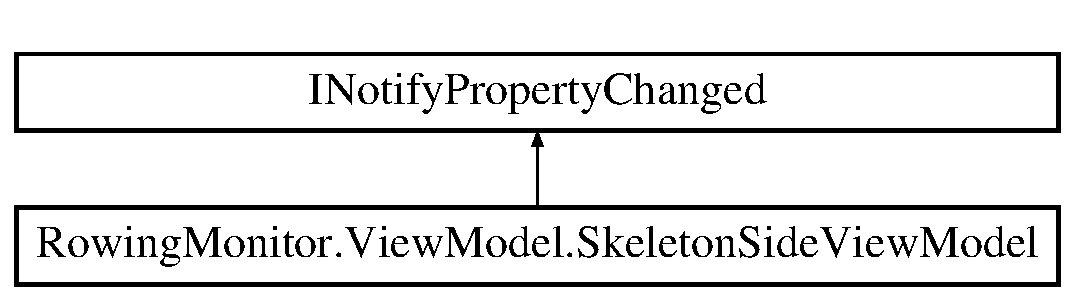
\includegraphics[height=2.000000cm]{class_rowing_monitor_1_1_view_model_1_1_skeleton_side_view_model}
\end{center}
\end{figure}
\subsection*{Public Member Functions}
\begin{DoxyCompactItemize}
\item 
\hyperlink{class_rowing_monitor_1_1_view_model_1_1_skeleton_side_view_model_aaf6f6d342b3351dfb98a8ba2a9936576}{Skeleton\+Side\+View\+Model} ()
\item 
void \hyperlink{class_rowing_monitor_1_1_view_model_1_1_skeleton_side_view_model_a3df8c93f7db5e5508fa9e219731aac91}{Render} ()
\item 
void \hyperlink{class_rowing_monitor_1_1_view_model_1_1_skeleton_side_view_model_a7dd65caa2dce80fa0761deb9601aabc1}{Update\+Skeleton\+Image} (Drawing\+Image skeleton\+Image\+Source)
\end{DoxyCompactItemize}
\subsection*{Properties}
\begin{DoxyCompactItemize}
\item 
Image\+Source \hyperlink{class_rowing_monitor_1_1_view_model_1_1_skeleton_side_view_model_a7e03d4603839dcdc9d5d4185b8deb496}{Skeleton\+Image\+Source}\hspace{0.3cm}{\ttfamily  \mbox{[}get, set\mbox{]}}
\item 
\hyperlink{class_rowing_monitor_1_1_model_1_1_pipeline_1_1_skeleton_side_display}{Skeleton\+Side\+Display} \hyperlink{class_rowing_monitor_1_1_view_model_1_1_skeleton_side_view_model_a57efea54b412831f6940cd8e5e8c101e}{Model}\hspace{0.3cm}{\ttfamily  \mbox{[}get, set\mbox{]}}
\end{DoxyCompactItemize}
\subsection*{Events}
\begin{DoxyCompactItemize}
\item 
Property\+Changed\+Event\+Handler \hyperlink{class_rowing_monitor_1_1_view_model_1_1_skeleton_side_view_model_a55f1fd445df598e35e9d6e1caf98a24d}{Property\+Changed}
\end{DoxyCompactItemize}


\subsection{Constructor \& Destructor Documentation}
\mbox{\Hypertarget{class_rowing_monitor_1_1_view_model_1_1_skeleton_side_view_model_aaf6f6d342b3351dfb98a8ba2a9936576}\label{class_rowing_monitor_1_1_view_model_1_1_skeleton_side_view_model_aaf6f6d342b3351dfb98a8ba2a9936576}} 
\index{Rowing\+Monitor\+::\+View\+Model\+::\+Skeleton\+Side\+View\+Model@{Rowing\+Monitor\+::\+View\+Model\+::\+Skeleton\+Side\+View\+Model}!Skeleton\+Side\+View\+Model@{Skeleton\+Side\+View\+Model}}
\index{Skeleton\+Side\+View\+Model@{Skeleton\+Side\+View\+Model}!Rowing\+Monitor\+::\+View\+Model\+::\+Skeleton\+Side\+View\+Model@{Rowing\+Monitor\+::\+View\+Model\+::\+Skeleton\+Side\+View\+Model}}
\subsubsection{\texorpdfstring{Skeleton\+Side\+View\+Model()}{SkeletonSideViewModel()}}
{\footnotesize\ttfamily Rowing\+Monitor.\+View\+Model.\+Skeleton\+Side\+View\+Model.\+Skeleton\+Side\+View\+Model (\begin{DoxyParamCaption}{ }\end{DoxyParamCaption})}



\subsection{Member Function Documentation}
\mbox{\Hypertarget{class_rowing_monitor_1_1_view_model_1_1_skeleton_side_view_model_a3df8c93f7db5e5508fa9e219731aac91}\label{class_rowing_monitor_1_1_view_model_1_1_skeleton_side_view_model_a3df8c93f7db5e5508fa9e219731aac91}} 
\index{Rowing\+Monitor\+::\+View\+Model\+::\+Skeleton\+Side\+View\+Model@{Rowing\+Monitor\+::\+View\+Model\+::\+Skeleton\+Side\+View\+Model}!Render@{Render}}
\index{Render@{Render}!Rowing\+Monitor\+::\+View\+Model\+::\+Skeleton\+Side\+View\+Model@{Rowing\+Monitor\+::\+View\+Model\+::\+Skeleton\+Side\+View\+Model}}
\subsubsection{\texorpdfstring{Render()}{Render()}}
{\footnotesize\ttfamily void Rowing\+Monitor.\+View\+Model.\+Skeleton\+Side\+View\+Model.\+Render (\begin{DoxyParamCaption}{ }\end{DoxyParamCaption})}

\mbox{\Hypertarget{class_rowing_monitor_1_1_view_model_1_1_skeleton_side_view_model_a7dd65caa2dce80fa0761deb9601aabc1}\label{class_rowing_monitor_1_1_view_model_1_1_skeleton_side_view_model_a7dd65caa2dce80fa0761deb9601aabc1}} 
\index{Rowing\+Monitor\+::\+View\+Model\+::\+Skeleton\+Side\+View\+Model@{Rowing\+Monitor\+::\+View\+Model\+::\+Skeleton\+Side\+View\+Model}!Update\+Skeleton\+Image@{Update\+Skeleton\+Image}}
\index{Update\+Skeleton\+Image@{Update\+Skeleton\+Image}!Rowing\+Monitor\+::\+View\+Model\+::\+Skeleton\+Side\+View\+Model@{Rowing\+Monitor\+::\+View\+Model\+::\+Skeleton\+Side\+View\+Model}}
\subsubsection{\texorpdfstring{Update\+Skeleton\+Image()}{UpdateSkeletonImage()}}
{\footnotesize\ttfamily void Rowing\+Monitor.\+View\+Model.\+Skeleton\+Side\+View\+Model.\+Update\+Skeleton\+Image (\begin{DoxyParamCaption}\item[{Drawing\+Image}]{skeleton\+Image\+Source }\end{DoxyParamCaption})}



\subsection{Property Documentation}
\mbox{\Hypertarget{class_rowing_monitor_1_1_view_model_1_1_skeleton_side_view_model_a57efea54b412831f6940cd8e5e8c101e}\label{class_rowing_monitor_1_1_view_model_1_1_skeleton_side_view_model_a57efea54b412831f6940cd8e5e8c101e}} 
\index{Rowing\+Monitor\+::\+View\+Model\+::\+Skeleton\+Side\+View\+Model@{Rowing\+Monitor\+::\+View\+Model\+::\+Skeleton\+Side\+View\+Model}!Model@{Model}}
\index{Model@{Model}!Rowing\+Monitor\+::\+View\+Model\+::\+Skeleton\+Side\+View\+Model@{Rowing\+Monitor\+::\+View\+Model\+::\+Skeleton\+Side\+View\+Model}}
\subsubsection{\texorpdfstring{Model}{Model}}
{\footnotesize\ttfamily \hyperlink{class_rowing_monitor_1_1_model_1_1_pipeline_1_1_skeleton_side_display}{Skeleton\+Side\+Display} Rowing\+Monitor.\+View\+Model.\+Skeleton\+Side\+View\+Model.\+Model\hspace{0.3cm}{\ttfamily [get]}, {\ttfamily [set]}}

\mbox{\Hypertarget{class_rowing_monitor_1_1_view_model_1_1_skeleton_side_view_model_a7e03d4603839dcdc9d5d4185b8deb496}\label{class_rowing_monitor_1_1_view_model_1_1_skeleton_side_view_model_a7e03d4603839dcdc9d5d4185b8deb496}} 
\index{Rowing\+Monitor\+::\+View\+Model\+::\+Skeleton\+Side\+View\+Model@{Rowing\+Monitor\+::\+View\+Model\+::\+Skeleton\+Side\+View\+Model}!Skeleton\+Image\+Source@{Skeleton\+Image\+Source}}
\index{Skeleton\+Image\+Source@{Skeleton\+Image\+Source}!Rowing\+Monitor\+::\+View\+Model\+::\+Skeleton\+Side\+View\+Model@{Rowing\+Monitor\+::\+View\+Model\+::\+Skeleton\+Side\+View\+Model}}
\subsubsection{\texorpdfstring{Skeleton\+Image\+Source}{SkeletonImageSource}}
{\footnotesize\ttfamily Image\+Source Rowing\+Monitor.\+View\+Model.\+Skeleton\+Side\+View\+Model.\+Skeleton\+Image\+Source\hspace{0.3cm}{\ttfamily [get]}, {\ttfamily [set]}}



\subsection{Event Documentation}
\mbox{\Hypertarget{class_rowing_monitor_1_1_view_model_1_1_skeleton_side_view_model_a55f1fd445df598e35e9d6e1caf98a24d}\label{class_rowing_monitor_1_1_view_model_1_1_skeleton_side_view_model_a55f1fd445df598e35e9d6e1caf98a24d}} 
\index{Rowing\+Monitor\+::\+View\+Model\+::\+Skeleton\+Side\+View\+Model@{Rowing\+Monitor\+::\+View\+Model\+::\+Skeleton\+Side\+View\+Model}!Property\+Changed@{Property\+Changed}}
\index{Property\+Changed@{Property\+Changed}!Rowing\+Monitor\+::\+View\+Model\+::\+Skeleton\+Side\+View\+Model@{Rowing\+Monitor\+::\+View\+Model\+::\+Skeleton\+Side\+View\+Model}}
\subsubsection{\texorpdfstring{Property\+Changed}{PropertyChanged}}
{\footnotesize\ttfamily Property\+Changed\+Event\+Handler Rowing\+Monitor.\+View\+Model.\+Skeleton\+Side\+View\+Model.\+Property\+Changed}



The documentation for this class was generated from the following file\+:\begin{DoxyCompactItemize}
\item 
View\+Model/\hyperlink{_skeleton_side_view_model_8cs}{Skeleton\+Side\+View\+Model.\+cs}\end{DoxyCompactItemize}

\hypertarget{class_rowing_monitor_1_1_model_1_1_smoothed_frame_arrived_event_args}{}\section{Rowing\+Monitor.\+Model.\+Smoothed\+Frame\+Arrived\+Event\+Args Class Reference}
\label{class_rowing_monitor_1_1_model_1_1_smoothed_frame_arrived_event_args}\index{Rowing\+Monitor.\+Model.\+Smoothed\+Frame\+Arrived\+Event\+Args@{Rowing\+Monitor.\+Model.\+Smoothed\+Frame\+Arrived\+Event\+Args}}


Represents the arguments for a smoothed joint data arrived event.  


Inheritance diagram for Rowing\+Monitor.\+Model.\+Smoothed\+Frame\+Arrived\+Event\+Args\+:\begin{figure}[H]
\begin{center}
\leavevmode
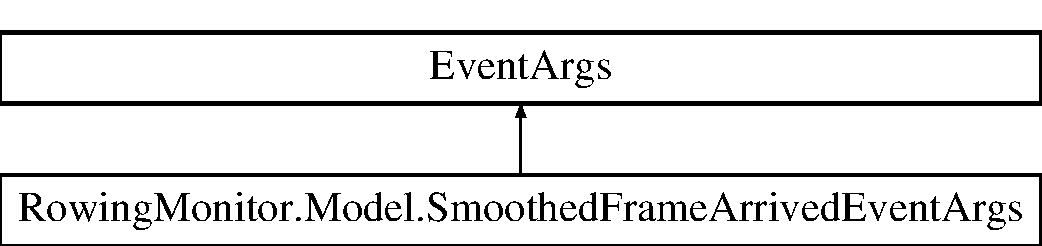
\includegraphics[height=2.000000cm]{class_rowing_monitor_1_1_model_1_1_smoothed_frame_arrived_event_args}
\end{center}
\end{figure}
\subsection*{Public Member Functions}
\begin{DoxyCompactItemize}
\item 
\hyperlink{class_rowing_monitor_1_1_model_1_1_smoothed_frame_arrived_event_args_a923725ca3400f634d0ce4a01c03388e7}{Smoothed\+Frame\+Arrived\+Event\+Args} (\hyperlink{struct_rowing_monitor_1_1_model_1_1_util_1_1_joint_data}{Joint\+Data} raw\+Joint\+Data, \hyperlink{struct_rowing_monitor_1_1_model_1_1_util_1_1_joint_data}{Joint\+Data} smoothed\+Joint\+Data)
\end{DoxyCompactItemize}
\subsection*{Properties}
\begin{DoxyCompactItemize}
\item 
\hyperlink{struct_rowing_monitor_1_1_model_1_1_util_1_1_joint_data}{Joint\+Data} \hyperlink{class_rowing_monitor_1_1_model_1_1_smoothed_frame_arrived_event_args_ae8c8a6d20114b898e9192ed282393178}{Raw\+Joint\+Data}\hspace{0.3cm}{\ttfamily  \mbox{[}get\mbox{]}}
\item 
\hyperlink{struct_rowing_monitor_1_1_model_1_1_util_1_1_joint_data}{Joint\+Data} \hyperlink{class_rowing_monitor_1_1_model_1_1_smoothed_frame_arrived_event_args_adee9a15912d769914f058a7e984948d6}{Smoothed\+Joint\+Data}\hspace{0.3cm}{\ttfamily  \mbox{[}get\mbox{]}}
\end{DoxyCompactItemize}


\subsection{Detailed Description}
Represents the arguments for a smoothed joint data arrived event. 



\subsection{Constructor \& Destructor Documentation}
\mbox{\Hypertarget{class_rowing_monitor_1_1_model_1_1_smoothed_frame_arrived_event_args_a923725ca3400f634d0ce4a01c03388e7}\label{class_rowing_monitor_1_1_model_1_1_smoothed_frame_arrived_event_args_a923725ca3400f634d0ce4a01c03388e7}} 
\index{Rowing\+Monitor\+::\+Model\+::\+Smoothed\+Frame\+Arrived\+Event\+Args@{Rowing\+Monitor\+::\+Model\+::\+Smoothed\+Frame\+Arrived\+Event\+Args}!Smoothed\+Frame\+Arrived\+Event\+Args@{Smoothed\+Frame\+Arrived\+Event\+Args}}
\index{Smoothed\+Frame\+Arrived\+Event\+Args@{Smoothed\+Frame\+Arrived\+Event\+Args}!Rowing\+Monitor\+::\+Model\+::\+Smoothed\+Frame\+Arrived\+Event\+Args@{Rowing\+Monitor\+::\+Model\+::\+Smoothed\+Frame\+Arrived\+Event\+Args}}
\subsubsection{\texorpdfstring{Smoothed\+Frame\+Arrived\+Event\+Args()}{SmoothedFrameArrivedEventArgs()}}
{\footnotesize\ttfamily Rowing\+Monitor.\+Model.\+Smoothed\+Frame\+Arrived\+Event\+Args.\+Smoothed\+Frame\+Arrived\+Event\+Args (\begin{DoxyParamCaption}\item[{\hyperlink{struct_rowing_monitor_1_1_model_1_1_util_1_1_joint_data}{Joint\+Data}}]{raw\+Joint\+Data,  }\item[{\hyperlink{struct_rowing_monitor_1_1_model_1_1_util_1_1_joint_data}{Joint\+Data}}]{smoothed\+Joint\+Data }\end{DoxyParamCaption})}



\subsection{Property Documentation}
\mbox{\Hypertarget{class_rowing_monitor_1_1_model_1_1_smoothed_frame_arrived_event_args_ae8c8a6d20114b898e9192ed282393178}\label{class_rowing_monitor_1_1_model_1_1_smoothed_frame_arrived_event_args_ae8c8a6d20114b898e9192ed282393178}} 
\index{Rowing\+Monitor\+::\+Model\+::\+Smoothed\+Frame\+Arrived\+Event\+Args@{Rowing\+Monitor\+::\+Model\+::\+Smoothed\+Frame\+Arrived\+Event\+Args}!Raw\+Joint\+Data@{Raw\+Joint\+Data}}
\index{Raw\+Joint\+Data@{Raw\+Joint\+Data}!Rowing\+Monitor\+::\+Model\+::\+Smoothed\+Frame\+Arrived\+Event\+Args@{Rowing\+Monitor\+::\+Model\+::\+Smoothed\+Frame\+Arrived\+Event\+Args}}
\subsubsection{\texorpdfstring{Raw\+Joint\+Data}{RawJointData}}
{\footnotesize\ttfamily \hyperlink{struct_rowing_monitor_1_1_model_1_1_util_1_1_joint_data}{Joint\+Data} Rowing\+Monitor.\+Model.\+Smoothed\+Frame\+Arrived\+Event\+Args.\+Raw\+Joint\+Data\hspace{0.3cm}{\ttfamily [get]}}

\mbox{\Hypertarget{class_rowing_monitor_1_1_model_1_1_smoothed_frame_arrived_event_args_adee9a15912d769914f058a7e984948d6}\label{class_rowing_monitor_1_1_model_1_1_smoothed_frame_arrived_event_args_adee9a15912d769914f058a7e984948d6}} 
\index{Rowing\+Monitor\+::\+Model\+::\+Smoothed\+Frame\+Arrived\+Event\+Args@{Rowing\+Monitor\+::\+Model\+::\+Smoothed\+Frame\+Arrived\+Event\+Args}!Smoothed\+Joint\+Data@{Smoothed\+Joint\+Data}}
\index{Smoothed\+Joint\+Data@{Smoothed\+Joint\+Data}!Rowing\+Monitor\+::\+Model\+::\+Smoothed\+Frame\+Arrived\+Event\+Args@{Rowing\+Monitor\+::\+Model\+::\+Smoothed\+Frame\+Arrived\+Event\+Args}}
\subsubsection{\texorpdfstring{Smoothed\+Joint\+Data}{SmoothedJointData}}
{\footnotesize\ttfamily \hyperlink{struct_rowing_monitor_1_1_model_1_1_util_1_1_joint_data}{Joint\+Data} Rowing\+Monitor.\+Model.\+Smoothed\+Frame\+Arrived\+Event\+Args.\+Smoothed\+Joint\+Data\hspace{0.3cm}{\ttfamily [get]}}



The documentation for this class was generated from the following file\+:\begin{DoxyCompactItemize}
\item 
Model/\+Event\+Args/\hyperlink{_smoothed_frame_arrived_event_args_8cs}{Smoothed\+Frame\+Arrived\+Event\+Args.\+cs}\end{DoxyCompactItemize}

\hypertarget{class_rowing_monitor_1_1_model_1_1_pipeline_1_1_smoothing_filter}{}\section{Rowing\+Monitor.\+Model.\+Pipeline.\+Smoothing\+Filter Class Reference}
\label{class_rowing_monitor_1_1_model_1_1_pipeline_1_1_smoothing_filter}\index{Rowing\+Monitor.\+Model.\+Pipeline.\+Smoothing\+Filter@{Rowing\+Monitor.\+Model.\+Pipeline.\+Smoothing\+Filter}}
Inheritance diagram for Rowing\+Monitor.\+Model.\+Pipeline.\+Smoothing\+Filter\+:\begin{figure}[H]
\begin{center}
\leavevmode
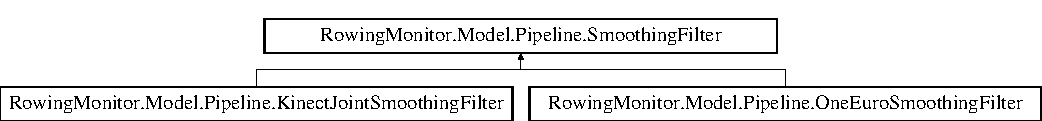
\includegraphics[height=1.623188cm]{class_rowing_monitor_1_1_model_1_1_pipeline_1_1_smoothing_filter}
\end{center}
\end{figure}
\subsection*{Public Member Functions}
\begin{DoxyCompactItemize}
\item 
delegate void \hyperlink{class_rowing_monitor_1_1_model_1_1_pipeline_1_1_smoothing_filter_af8a8a5758bd7a174033f698dcb1b93b2}{Smoothed\+Frame\+Arrived\+Event\+Handler} (Object sender, \hyperlink{class_rowing_monitor_1_1_model_1_1_smoothed_frame_arrived_event_args}{Smoothed\+Frame\+Arrived\+Event\+Args} e)
\item 
abstract \hyperlink{struct_rowing_monitor_1_1_model_1_1_util_1_1_joint_data}{Joint\+Data} \hyperlink{class_rowing_monitor_1_1_model_1_1_pipeline_1_1_smoothing_filter_a65ba6a5a48fbf5a51fb564dbeefc95fe}{Smooth} (\hyperlink{struct_rowing_monitor_1_1_model_1_1_util_1_1_joint_data}{Joint\+Data} joint\+Data)
\item 
abstract void \hyperlink{class_rowing_monitor_1_1_model_1_1_pipeline_1_1_smoothing_filter_a6f017782fee0747d4ece9ec3ffea6115}{Update} (\hyperlink{struct_rowing_monitor_1_1_model_1_1_util_1_1_joint_data}{Joint\+Data} joint\+Data)
\end{DoxyCompactItemize}
\subsection*{Protected Member Functions}
\begin{DoxyCompactItemize}
\item 
virtual void \hyperlink{class_rowing_monitor_1_1_model_1_1_pipeline_1_1_smoothing_filter_ac47b399ad4ae1ad899f5e571d6f6c05c}{On\+Smoothed\+Frame\+Finished} (\hyperlink{class_rowing_monitor_1_1_model_1_1_smoothed_frame_arrived_event_args}{Smoothed\+Frame\+Arrived\+Event\+Args} e)
\end{DoxyCompactItemize}
\subsection*{Properties}
\begin{DoxyCompactItemize}
\item 
Broadcast\+Block$<$ \hyperlink{struct_rowing_monitor_1_1_model_1_1_util_1_1_joint_data}{Joint\+Data} $>$ \hyperlink{class_rowing_monitor_1_1_model_1_1_pipeline_1_1_smoothing_filter_a3151be406d68f220c45b674df65f0df5}{Output}\hspace{0.3cm}{\ttfamily  \mbox{[}get, set\mbox{]}}
\item 
\hyperlink{namespace_rowing_monitor_1_1_model_1_1_util_a01e1a06061533b246feb7421c9d0107f}{Data\+Stream\+Type} \hyperlink{class_rowing_monitor_1_1_model_1_1_pipeline_1_1_smoothing_filter_a25304d8ea2f3e1f80ab786fb40bca304}{Output\+Data\+Stream\+Type}\hspace{0.3cm}{\ttfamily  \mbox{[}get, set\mbox{]}}
\item 
Action\+Block$<$ \hyperlink{struct_rowing_monitor_1_1_model_1_1_util_1_1_joint_data}{Joint\+Data} $>$ \hyperlink{class_rowing_monitor_1_1_model_1_1_pipeline_1_1_smoothing_filter_a92bef5838dd409b0795f5b94c1ea45d5}{Input}\hspace{0.3cm}{\ttfamily  \mbox{[}get, set\mbox{]}}
\end{DoxyCompactItemize}
\subsection*{Events}
\begin{DoxyCompactItemize}
\item 
\hyperlink{class_rowing_monitor_1_1_model_1_1_pipeline_1_1_smoothing_filter_af8a8a5758bd7a174033f698dcb1b93b2}{Smoothed\+Frame\+Arrived\+Event\+Handler} \hyperlink{class_rowing_monitor_1_1_model_1_1_pipeline_1_1_smoothing_filter_adfb76570d0a85e7cfd41d16121ce7a56}{Smoothed\+Frame\+Arrived}
\end{DoxyCompactItemize}


\subsection{Member Function Documentation}
\mbox{\Hypertarget{class_rowing_monitor_1_1_model_1_1_pipeline_1_1_smoothing_filter_ac47b399ad4ae1ad899f5e571d6f6c05c}\label{class_rowing_monitor_1_1_model_1_1_pipeline_1_1_smoothing_filter_ac47b399ad4ae1ad899f5e571d6f6c05c}} 
\index{Rowing\+Monitor\+::\+Model\+::\+Pipeline\+::\+Smoothing\+Filter@{Rowing\+Monitor\+::\+Model\+::\+Pipeline\+::\+Smoothing\+Filter}!On\+Smoothed\+Frame\+Finished@{On\+Smoothed\+Frame\+Finished}}
\index{On\+Smoothed\+Frame\+Finished@{On\+Smoothed\+Frame\+Finished}!Rowing\+Monitor\+::\+Model\+::\+Pipeline\+::\+Smoothing\+Filter@{Rowing\+Monitor\+::\+Model\+::\+Pipeline\+::\+Smoothing\+Filter}}
\subsubsection{\texorpdfstring{On\+Smoothed\+Frame\+Finished()}{OnSmoothedFrameFinished()}}
{\footnotesize\ttfamily virtual void Rowing\+Monitor.\+Model.\+Pipeline.\+Smoothing\+Filter.\+On\+Smoothed\+Frame\+Finished (\begin{DoxyParamCaption}\item[{\hyperlink{class_rowing_monitor_1_1_model_1_1_smoothed_frame_arrived_event_args}{Smoothed\+Frame\+Arrived\+Event\+Args}}]{e }\end{DoxyParamCaption})\hspace{0.3cm}{\ttfamily [protected]}, {\ttfamily [virtual]}}



Reimplemented in \hyperlink{class_rowing_monitor_1_1_model_1_1_pipeline_1_1_kinect_joint_smoothing_filter_a944294caee0b2b26c0023a1c2d0c1a67}{Rowing\+Monitor.\+Model.\+Pipeline.\+Kinect\+Joint\+Smoothing\+Filter}, and \hyperlink{class_rowing_monitor_1_1_model_1_1_pipeline_1_1_one_euro_smoothing_filter_ab4f64e95b9e02fb1562aeee79a75e695}{Rowing\+Monitor.\+Model.\+Pipeline.\+One\+Euro\+Smoothing\+Filter}.

\mbox{\Hypertarget{class_rowing_monitor_1_1_model_1_1_pipeline_1_1_smoothing_filter_a65ba6a5a48fbf5a51fb564dbeefc95fe}\label{class_rowing_monitor_1_1_model_1_1_pipeline_1_1_smoothing_filter_a65ba6a5a48fbf5a51fb564dbeefc95fe}} 
\index{Rowing\+Monitor\+::\+Model\+::\+Pipeline\+::\+Smoothing\+Filter@{Rowing\+Monitor\+::\+Model\+::\+Pipeline\+::\+Smoothing\+Filter}!Smooth@{Smooth}}
\index{Smooth@{Smooth}!Rowing\+Monitor\+::\+Model\+::\+Pipeline\+::\+Smoothing\+Filter@{Rowing\+Monitor\+::\+Model\+::\+Pipeline\+::\+Smoothing\+Filter}}
\subsubsection{\texorpdfstring{Smooth()}{Smooth()}}
{\footnotesize\ttfamily abstract \hyperlink{struct_rowing_monitor_1_1_model_1_1_util_1_1_joint_data}{Joint\+Data} Rowing\+Monitor.\+Model.\+Pipeline.\+Smoothing\+Filter.\+Smooth (\begin{DoxyParamCaption}\item[{\hyperlink{struct_rowing_monitor_1_1_model_1_1_util_1_1_joint_data}{Joint\+Data}}]{joint\+Data }\end{DoxyParamCaption})\hspace{0.3cm}{\ttfamily [pure virtual]}}



Implemented in \hyperlink{class_rowing_monitor_1_1_model_1_1_pipeline_1_1_kinect_joint_smoothing_filter_a31ee74610f6c7de082306691f59d2f1c}{Rowing\+Monitor.\+Model.\+Pipeline.\+Kinect\+Joint\+Smoothing\+Filter}, and \hyperlink{class_rowing_monitor_1_1_model_1_1_pipeline_1_1_one_euro_smoothing_filter_afd860237def583deb4499bc3c9fac868}{Rowing\+Monitor.\+Model.\+Pipeline.\+One\+Euro\+Smoothing\+Filter}.

\mbox{\Hypertarget{class_rowing_monitor_1_1_model_1_1_pipeline_1_1_smoothing_filter_af8a8a5758bd7a174033f698dcb1b93b2}\label{class_rowing_monitor_1_1_model_1_1_pipeline_1_1_smoothing_filter_af8a8a5758bd7a174033f698dcb1b93b2}} 
\index{Rowing\+Monitor\+::\+Model\+::\+Pipeline\+::\+Smoothing\+Filter@{Rowing\+Monitor\+::\+Model\+::\+Pipeline\+::\+Smoothing\+Filter}!Smoothed\+Frame\+Arrived\+Event\+Handler@{Smoothed\+Frame\+Arrived\+Event\+Handler}}
\index{Smoothed\+Frame\+Arrived\+Event\+Handler@{Smoothed\+Frame\+Arrived\+Event\+Handler}!Rowing\+Monitor\+::\+Model\+::\+Pipeline\+::\+Smoothing\+Filter@{Rowing\+Monitor\+::\+Model\+::\+Pipeline\+::\+Smoothing\+Filter}}
\subsubsection{\texorpdfstring{Smoothed\+Frame\+Arrived\+Event\+Handler()}{SmoothedFrameArrivedEventHandler()}}
{\footnotesize\ttfamily delegate void Rowing\+Monitor.\+Model.\+Pipeline.\+Smoothing\+Filter.\+Smoothed\+Frame\+Arrived\+Event\+Handler (\begin{DoxyParamCaption}\item[{Object}]{sender,  }\item[{\hyperlink{class_rowing_monitor_1_1_model_1_1_smoothed_frame_arrived_event_args}{Smoothed\+Frame\+Arrived\+Event\+Args}}]{e }\end{DoxyParamCaption})}

\mbox{\Hypertarget{class_rowing_monitor_1_1_model_1_1_pipeline_1_1_smoothing_filter_a6f017782fee0747d4ece9ec3ffea6115}\label{class_rowing_monitor_1_1_model_1_1_pipeline_1_1_smoothing_filter_a6f017782fee0747d4ece9ec3ffea6115}} 
\index{Rowing\+Monitor\+::\+Model\+::\+Pipeline\+::\+Smoothing\+Filter@{Rowing\+Monitor\+::\+Model\+::\+Pipeline\+::\+Smoothing\+Filter}!Update@{Update}}
\index{Update@{Update}!Rowing\+Monitor\+::\+Model\+::\+Pipeline\+::\+Smoothing\+Filter@{Rowing\+Monitor\+::\+Model\+::\+Pipeline\+::\+Smoothing\+Filter}}
\subsubsection{\texorpdfstring{Update()}{Update()}}
{\footnotesize\ttfamily abstract void Rowing\+Monitor.\+Model.\+Pipeline.\+Smoothing\+Filter.\+Update (\begin{DoxyParamCaption}\item[{\hyperlink{struct_rowing_monitor_1_1_model_1_1_util_1_1_joint_data}{Joint\+Data}}]{joint\+Data }\end{DoxyParamCaption})\hspace{0.3cm}{\ttfamily [pure virtual]}}



Implemented in \hyperlink{class_rowing_monitor_1_1_model_1_1_pipeline_1_1_kinect_joint_smoothing_filter_a93cb6db0e00796dd2791789e472457b5}{Rowing\+Monitor.\+Model.\+Pipeline.\+Kinect\+Joint\+Smoothing\+Filter}, and \hyperlink{class_rowing_monitor_1_1_model_1_1_pipeline_1_1_one_euro_smoothing_filter_a2e518ce98440b3004aaf1af9a4eba399}{Rowing\+Monitor.\+Model.\+Pipeline.\+One\+Euro\+Smoothing\+Filter}.



\subsection{Property Documentation}
\mbox{\Hypertarget{class_rowing_monitor_1_1_model_1_1_pipeline_1_1_smoothing_filter_a92bef5838dd409b0795f5b94c1ea45d5}\label{class_rowing_monitor_1_1_model_1_1_pipeline_1_1_smoothing_filter_a92bef5838dd409b0795f5b94c1ea45d5}} 
\index{Rowing\+Monitor\+::\+Model\+::\+Pipeline\+::\+Smoothing\+Filter@{Rowing\+Monitor\+::\+Model\+::\+Pipeline\+::\+Smoothing\+Filter}!Input@{Input}}
\index{Input@{Input}!Rowing\+Monitor\+::\+Model\+::\+Pipeline\+::\+Smoothing\+Filter@{Rowing\+Monitor\+::\+Model\+::\+Pipeline\+::\+Smoothing\+Filter}}
\subsubsection{\texorpdfstring{Input}{Input}}
{\footnotesize\ttfamily Action\+Block$<$\hyperlink{struct_rowing_monitor_1_1_model_1_1_util_1_1_joint_data}{Joint\+Data}$>$ Rowing\+Monitor.\+Model.\+Pipeline.\+Smoothing\+Filter.\+Input\hspace{0.3cm}{\ttfamily [get]}, {\ttfamily [set]}}

\mbox{\Hypertarget{class_rowing_monitor_1_1_model_1_1_pipeline_1_1_smoothing_filter_a3151be406d68f220c45b674df65f0df5}\label{class_rowing_monitor_1_1_model_1_1_pipeline_1_1_smoothing_filter_a3151be406d68f220c45b674df65f0df5}} 
\index{Rowing\+Monitor\+::\+Model\+::\+Pipeline\+::\+Smoothing\+Filter@{Rowing\+Monitor\+::\+Model\+::\+Pipeline\+::\+Smoothing\+Filter}!Output@{Output}}
\index{Output@{Output}!Rowing\+Monitor\+::\+Model\+::\+Pipeline\+::\+Smoothing\+Filter@{Rowing\+Monitor\+::\+Model\+::\+Pipeline\+::\+Smoothing\+Filter}}
\subsubsection{\texorpdfstring{Output}{Output}}
{\footnotesize\ttfamily Broadcast\+Block$<$\hyperlink{struct_rowing_monitor_1_1_model_1_1_util_1_1_joint_data}{Joint\+Data}$>$ Rowing\+Monitor.\+Model.\+Pipeline.\+Smoothing\+Filter.\+Output\hspace{0.3cm}{\ttfamily [get]}, {\ttfamily [set]}}

\mbox{\Hypertarget{class_rowing_monitor_1_1_model_1_1_pipeline_1_1_smoothing_filter_a25304d8ea2f3e1f80ab786fb40bca304}\label{class_rowing_monitor_1_1_model_1_1_pipeline_1_1_smoothing_filter_a25304d8ea2f3e1f80ab786fb40bca304}} 
\index{Rowing\+Monitor\+::\+Model\+::\+Pipeline\+::\+Smoothing\+Filter@{Rowing\+Monitor\+::\+Model\+::\+Pipeline\+::\+Smoothing\+Filter}!Output\+Data\+Stream\+Type@{Output\+Data\+Stream\+Type}}
\index{Output\+Data\+Stream\+Type@{Output\+Data\+Stream\+Type}!Rowing\+Monitor\+::\+Model\+::\+Pipeline\+::\+Smoothing\+Filter@{Rowing\+Monitor\+::\+Model\+::\+Pipeline\+::\+Smoothing\+Filter}}
\subsubsection{\texorpdfstring{Output\+Data\+Stream\+Type}{OutputDataStreamType}}
{\footnotesize\ttfamily \hyperlink{namespace_rowing_monitor_1_1_model_1_1_util_a01e1a06061533b246feb7421c9d0107f}{Data\+Stream\+Type} Rowing\+Monitor.\+Model.\+Pipeline.\+Smoothing\+Filter.\+Output\+Data\+Stream\+Type\hspace{0.3cm}{\ttfamily [get]}, {\ttfamily [set]}}



\subsection{Event Documentation}
\mbox{\Hypertarget{class_rowing_monitor_1_1_model_1_1_pipeline_1_1_smoothing_filter_adfb76570d0a85e7cfd41d16121ce7a56}\label{class_rowing_monitor_1_1_model_1_1_pipeline_1_1_smoothing_filter_adfb76570d0a85e7cfd41d16121ce7a56}} 
\index{Rowing\+Monitor\+::\+Model\+::\+Pipeline\+::\+Smoothing\+Filter@{Rowing\+Monitor\+::\+Model\+::\+Pipeline\+::\+Smoothing\+Filter}!Smoothed\+Frame\+Arrived@{Smoothed\+Frame\+Arrived}}
\index{Smoothed\+Frame\+Arrived@{Smoothed\+Frame\+Arrived}!Rowing\+Monitor\+::\+Model\+::\+Pipeline\+::\+Smoothing\+Filter@{Rowing\+Monitor\+::\+Model\+::\+Pipeline\+::\+Smoothing\+Filter}}
\subsubsection{\texorpdfstring{Smoothed\+Frame\+Arrived}{SmoothedFrameArrived}}
{\footnotesize\ttfamily \hyperlink{class_rowing_monitor_1_1_model_1_1_pipeline_1_1_smoothing_filter_af8a8a5758bd7a174033f698dcb1b93b2}{Smoothed\+Frame\+Arrived\+Event\+Handler} Rowing\+Monitor.\+Model.\+Pipeline.\+Smoothing\+Filter.\+Smoothed\+Frame\+Arrived}



The documentation for this class was generated from the following file\+:\begin{DoxyCompactItemize}
\item 
Model/\+Pipeline/\hyperlink{_smoothing_filter_8cs}{Smoothing\+Filter.\+cs}\end{DoxyCompactItemize}

\hypertarget{struct_rowing_monitor_1_1_model_1_1_util_1_1_subsequence}{}\section{Rowing\+Monitor.\+Model.\+Util.\+Subsequence Struct Reference}
\label{struct_rowing_monitor_1_1_model_1_1_util_1_1_subsequence}\index{Rowing\+Monitor.\+Model.\+Util.\+Subsequence@{Rowing\+Monitor.\+Model.\+Util.\+Subsequence}}


\hyperlink{struct_rowing_monitor_1_1_model_1_1_util_1_1_subsequence}{Subsequence} in a data stream which suits a given template.  


\subsection*{Properties}
\begin{DoxyCompactItemize}
\item 
double \hyperlink{struct_rowing_monitor_1_1_model_1_1_util_1_1_subsequence_a9f07ec73d4dcc7cb1d9e97f7e979fcc1}{Distance}\hspace{0.3cm}{\ttfamily  \mbox{[}get, set\mbox{]}}
\begin{DoxyCompactList}\small\item\em Calculates distance between the template and the data stream. \end{DoxyCompactList}\item 
int \hyperlink{struct_rowing_monitor_1_1_model_1_1_util_1_1_subsequence_af085c001955793f45836d6c1cf3d4882}{T\+Start}\hspace{0.3cm}{\ttfamily  \mbox{[}get, set\mbox{]}}
\begin{DoxyCompactList}\small\item\em Starttime of data stream which fits to the template. \end{DoxyCompactList}\item 
int \hyperlink{struct_rowing_monitor_1_1_model_1_1_util_1_1_subsequence_a839b2f62176c2546a8e0d42b87801954}{T\+End}\hspace{0.3cm}{\ttfamily  \mbox{[}get, set\mbox{]}}
\begin{DoxyCompactList}\small\item\em Endtime of data stream which fits to the template. \end{DoxyCompactList}\item 
\hyperlink{namespace_rowing_monitor_1_1_model_1_1_util_a248a257b884983ed79c45a8b34ee9580}{Subsequence\+Status} \hyperlink{struct_rowing_monitor_1_1_model_1_1_util_1_1_subsequence_a437775e5f7ee4b63b6a33a01ef46bf0c}{Status}\hspace{0.3cm}{\ttfamily  \mbox{[}get, set\mbox{]}}
\begin{DoxyCompactList}\small\item\em Status of detected subsequence. \end{DoxyCompactList}\item 
int \hyperlink{struct_rowing_monitor_1_1_model_1_1_util_1_1_subsequence_aaaed8840b79d2c683073ecf408bc6d51}{T\+Detected}\hspace{0.3cm}{\ttfamily  \mbox{[}get, set\mbox{]}}
\begin{DoxyCompactList}\small\item\em Time of detection. \end{DoxyCompactList}\end{DoxyCompactItemize}


\subsection{Detailed Description}
\hyperlink{struct_rowing_monitor_1_1_model_1_1_util_1_1_subsequence}{Subsequence} in a data stream which suits a given template. 



\subsection{Property Documentation}
\mbox{\Hypertarget{struct_rowing_monitor_1_1_model_1_1_util_1_1_subsequence_a9f07ec73d4dcc7cb1d9e97f7e979fcc1}\label{struct_rowing_monitor_1_1_model_1_1_util_1_1_subsequence_a9f07ec73d4dcc7cb1d9e97f7e979fcc1}} 
\index{Rowing\+Monitor\+::\+Model\+::\+Util\+::\+Subsequence@{Rowing\+Monitor\+::\+Model\+::\+Util\+::\+Subsequence}!Distance@{Distance}}
\index{Distance@{Distance}!Rowing\+Monitor\+::\+Model\+::\+Util\+::\+Subsequence@{Rowing\+Monitor\+::\+Model\+::\+Util\+::\+Subsequence}}
\subsubsection{\texorpdfstring{Distance}{Distance}}
{\footnotesize\ttfamily double Rowing\+Monitor.\+Model.\+Util.\+Subsequence.\+Distance\hspace{0.3cm}{\ttfamily [get]}, {\ttfamily [set]}}



Calculates distance between the template and the data stream. 

\mbox{\Hypertarget{struct_rowing_monitor_1_1_model_1_1_util_1_1_subsequence_a437775e5f7ee4b63b6a33a01ef46bf0c}\label{struct_rowing_monitor_1_1_model_1_1_util_1_1_subsequence_a437775e5f7ee4b63b6a33a01ef46bf0c}} 
\index{Rowing\+Monitor\+::\+Model\+::\+Util\+::\+Subsequence@{Rowing\+Monitor\+::\+Model\+::\+Util\+::\+Subsequence}!Status@{Status}}
\index{Status@{Status}!Rowing\+Monitor\+::\+Model\+::\+Util\+::\+Subsequence@{Rowing\+Monitor\+::\+Model\+::\+Util\+::\+Subsequence}}
\subsubsection{\texorpdfstring{Status}{Status}}
{\footnotesize\ttfamily \hyperlink{namespace_rowing_monitor_1_1_model_1_1_util_a248a257b884983ed79c45a8b34ee9580}{Subsequence\+Status} Rowing\+Monitor.\+Model.\+Util.\+Subsequence.\+Status\hspace{0.3cm}{\ttfamily [get]}, {\ttfamily [set]}}



Status of detected subsequence. 

\mbox{\Hypertarget{struct_rowing_monitor_1_1_model_1_1_util_1_1_subsequence_aaaed8840b79d2c683073ecf408bc6d51}\label{struct_rowing_monitor_1_1_model_1_1_util_1_1_subsequence_aaaed8840b79d2c683073ecf408bc6d51}} 
\index{Rowing\+Monitor\+::\+Model\+::\+Util\+::\+Subsequence@{Rowing\+Monitor\+::\+Model\+::\+Util\+::\+Subsequence}!T\+Detected@{T\+Detected}}
\index{T\+Detected@{T\+Detected}!Rowing\+Monitor\+::\+Model\+::\+Util\+::\+Subsequence@{Rowing\+Monitor\+::\+Model\+::\+Util\+::\+Subsequence}}
\subsubsection{\texorpdfstring{T\+Detected}{TDetected}}
{\footnotesize\ttfamily int Rowing\+Monitor.\+Model.\+Util.\+Subsequence.\+T\+Detected\hspace{0.3cm}{\ttfamily [get]}, {\ttfamily [set]}}



Time of detection. 

\mbox{\Hypertarget{struct_rowing_monitor_1_1_model_1_1_util_1_1_subsequence_a839b2f62176c2546a8e0d42b87801954}\label{struct_rowing_monitor_1_1_model_1_1_util_1_1_subsequence_a839b2f62176c2546a8e0d42b87801954}} 
\index{Rowing\+Monitor\+::\+Model\+::\+Util\+::\+Subsequence@{Rowing\+Monitor\+::\+Model\+::\+Util\+::\+Subsequence}!T\+End@{T\+End}}
\index{T\+End@{T\+End}!Rowing\+Monitor\+::\+Model\+::\+Util\+::\+Subsequence@{Rowing\+Monitor\+::\+Model\+::\+Util\+::\+Subsequence}}
\subsubsection{\texorpdfstring{T\+End}{TEnd}}
{\footnotesize\ttfamily int Rowing\+Monitor.\+Model.\+Util.\+Subsequence.\+T\+End\hspace{0.3cm}{\ttfamily [get]}, {\ttfamily [set]}}



Endtime of data stream which fits to the template. 

\mbox{\Hypertarget{struct_rowing_monitor_1_1_model_1_1_util_1_1_subsequence_af085c001955793f45836d6c1cf3d4882}\label{struct_rowing_monitor_1_1_model_1_1_util_1_1_subsequence_af085c001955793f45836d6c1cf3d4882}} 
\index{Rowing\+Monitor\+::\+Model\+::\+Util\+::\+Subsequence@{Rowing\+Monitor\+::\+Model\+::\+Util\+::\+Subsequence}!T\+Start@{T\+Start}}
\index{T\+Start@{T\+Start}!Rowing\+Monitor\+::\+Model\+::\+Util\+::\+Subsequence@{Rowing\+Monitor\+::\+Model\+::\+Util\+::\+Subsequence}}
\subsubsection{\texorpdfstring{T\+Start}{TStart}}
{\footnotesize\ttfamily int Rowing\+Monitor.\+Model.\+Util.\+Subsequence.\+T\+Start\hspace{0.3cm}{\ttfamily [get]}, {\ttfamily [set]}}



Starttime of data stream which fits to the template. 



The documentation for this struct was generated from the following file\+:\begin{DoxyCompactItemize}
\item 
Model/\+Util/\hyperlink{_subsequence_d_t_w_8cs}{Subsequence\+D\+T\+W.\+cs}\end{DoxyCompactItemize}

\hypertarget{class_rowing_monitor_1_1_model_1_1_util_1_1_subsequence_d_t_w}{}\section{Rowing\+Monitor.\+Model.\+Util.\+Subsequence\+D\+TW Class Reference}
\label{class_rowing_monitor_1_1_model_1_1_util_1_1_subsequence_d_t_w}\index{Rowing\+Monitor.\+Model.\+Util.\+Subsequence\+D\+TW@{Rowing\+Monitor.\+Model.\+Util.\+Subsequence\+D\+TW}}


Compares an online data stream with a template stream. Uses the S\+P\+R\+I\+NG D\+TW algorithm.  


\subsection*{Public Member Functions}
\begin{DoxyCompactItemize}
\item 
\hyperlink{class_rowing_monitor_1_1_model_1_1_util_1_1_subsequence_d_t_w_a16ee898f6e11aee3d1b3ccfb482cdddb}{Subsequence\+D\+TW} (List$<$ double $>$ template, float distance\+Threshold, int minimum\+Subsequence\+Length=2)
\begin{DoxyCompactList}\small\item\em Creates a new instance of the \hyperlink{class_rowing_monitor_1_1_model_1_1_util_1_1_subsequence_d_t_w}{Subsequence\+D\+TW} class. \end{DoxyCompactList}\item 
\hyperlink{struct_rowing_monitor_1_1_model_1_1_util_1_1_subsequence}{Subsequence} \hyperlink{class_rowing_monitor_1_1_model_1_1_util_1_1_subsequence_d_t_w_a2aa9afce49cbb11a86ee3e5791397416}{compare\+Data\+Stream} (double xT, int t)
\begin{DoxyCompactList}\small\item\em Compare the value x at time t of the data stream with the template. Returns an unset, not optimal or optimal subsequence with its distance, starttime and endtime. Uses the S\+P\+R\+I\+NG D\+TW algorithm. \end{DoxyCompactList}\end{DoxyCompactItemize}


\subsection{Detailed Description}
Compares an online data stream with a template stream. Uses the S\+P\+R\+I\+NG D\+TW algorithm. 



\subsection{Constructor \& Destructor Documentation}
\mbox{\Hypertarget{class_rowing_monitor_1_1_model_1_1_util_1_1_subsequence_d_t_w_a16ee898f6e11aee3d1b3ccfb482cdddb}\label{class_rowing_monitor_1_1_model_1_1_util_1_1_subsequence_d_t_w_a16ee898f6e11aee3d1b3ccfb482cdddb}} 
\index{Rowing\+Monitor\+::\+Model\+::\+Util\+::\+Subsequence\+D\+TW@{Rowing\+Monitor\+::\+Model\+::\+Util\+::\+Subsequence\+D\+TW}!Subsequence\+D\+TW@{Subsequence\+D\+TW}}
\index{Subsequence\+D\+TW@{Subsequence\+D\+TW}!Rowing\+Monitor\+::\+Model\+::\+Util\+::\+Subsequence\+D\+TW@{Rowing\+Monitor\+::\+Model\+::\+Util\+::\+Subsequence\+D\+TW}}
\subsubsection{\texorpdfstring{Subsequence\+D\+T\+W()}{SubsequenceDTW()}}
{\footnotesize\ttfamily Rowing\+Monitor.\+Model.\+Util.\+Subsequence\+D\+T\+W.\+Subsequence\+D\+TW (\begin{DoxyParamCaption}\item[{List$<$ double $>$}]{template,  }\item[{float}]{distance\+Threshold,  }\item[{int}]{minimum\+Subsequence\+Length = {\ttfamily 2} }\end{DoxyParamCaption})}



Creates a new instance of the \hyperlink{class_rowing_monitor_1_1_model_1_1_util_1_1_subsequence_d_t_w}{Subsequence\+D\+TW} class. 


\begin{DoxyParams}{Parameters}
{\em template} & \\
\hline
\end{DoxyParams}
Template stream for comparison. 
\begin{DoxyParams}{Parameters}
{\em distance\+Threshold} & \\
\hline
\end{DoxyParams}
Distance threshold which describes the maximum distance that reports a detected subsequence. 
\begin{DoxyParams}{Parameters}
{\em minimum\+Subsequence\+Length} & \\
\hline
\end{DoxyParams}
Minimum length of a detected subsequence. 

\subsection{Member Function Documentation}
\mbox{\Hypertarget{class_rowing_monitor_1_1_model_1_1_util_1_1_subsequence_d_t_w_a2aa9afce49cbb11a86ee3e5791397416}\label{class_rowing_monitor_1_1_model_1_1_util_1_1_subsequence_d_t_w_a2aa9afce49cbb11a86ee3e5791397416}} 
\index{Rowing\+Monitor\+::\+Model\+::\+Util\+::\+Subsequence\+D\+TW@{Rowing\+Monitor\+::\+Model\+::\+Util\+::\+Subsequence\+D\+TW}!compare\+Data\+Stream@{compare\+Data\+Stream}}
\index{compare\+Data\+Stream@{compare\+Data\+Stream}!Rowing\+Monitor\+::\+Model\+::\+Util\+::\+Subsequence\+D\+TW@{Rowing\+Monitor\+::\+Model\+::\+Util\+::\+Subsequence\+D\+TW}}
\subsubsection{\texorpdfstring{compare\+Data\+Stream()}{compareDataStream()}}
{\footnotesize\ttfamily \hyperlink{struct_rowing_monitor_1_1_model_1_1_util_1_1_subsequence}{Subsequence} Rowing\+Monitor.\+Model.\+Util.\+Subsequence\+D\+T\+W.\+compare\+Data\+Stream (\begin{DoxyParamCaption}\item[{double}]{xT,  }\item[{int}]{t }\end{DoxyParamCaption})}



Compare the value x at time t of the data stream with the template. Returns an unset, not optimal or optimal subsequence with its distance, starttime and endtime. Uses the S\+P\+R\+I\+NG D\+TW algorithm. 


\begin{DoxyParams}{Parameters}
{\em xT} & \\
\hline
\end{DoxyParams}
Value x of data stream at time t. 
\begin{DoxyParams}{Parameters}
{\em t} & \\
\hline
\end{DoxyParams}
Time t of value x. Time starts with 1. \begin{DoxyReturn}{Returns}

\end{DoxyReturn}
A subsequence with its distance, starttime and endtime. 

The documentation for this class was generated from the following file\+:\begin{DoxyCompactItemize}
\item 
Model/\+Util/\hyperlink{_subsequence_d_t_w_8cs}{Subsequence\+D\+T\+W.\+cs}\end{DoxyCompactItemize}

\hypertarget{class_rowing_monitor_1_1_view_1_1_trainee_view}{}\section{Rowing\+Monitor.\+View.\+Trainee\+View Class Reference}
\label{class_rowing_monitor_1_1_view_1_1_trainee_view}\index{Rowing\+Monitor.\+View.\+Trainee\+View@{Rowing\+Monitor.\+View.\+Trainee\+View}}


\hyperlink{class_rowing_monitor_1_1_view_1_1_trainee_view}{Trainee\+View}  


Inheritance diagram for Rowing\+Monitor.\+View.\+Trainee\+View\+:\begin{figure}[H]
\begin{center}
\leavevmode
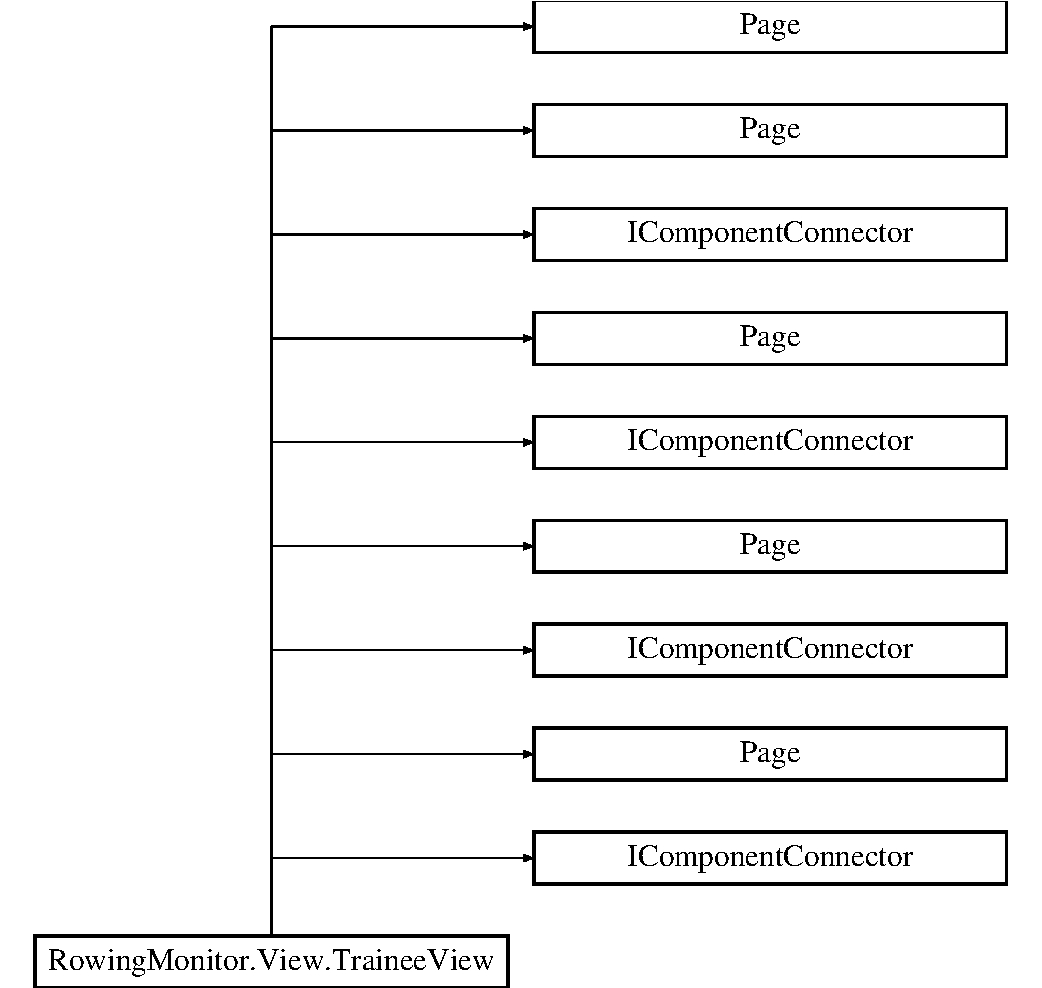
\includegraphics[height=10.000000cm]{class_rowing_monitor_1_1_view_1_1_trainee_view}
\end{center}
\end{figure}
\subsection*{Public Member Functions}
\begin{DoxyCompactItemize}
\item 
void \hyperlink{class_rowing_monitor_1_1_view_1_1_trainee_view_aafd3b2c6136bc2da309abd7b3706619a}{Initialize\+Component} ()
\begin{DoxyCompactList}\small\item\em Initialize\+Component \end{DoxyCompactList}\item 
void \hyperlink{class_rowing_monitor_1_1_view_1_1_trainee_view_aafd3b2c6136bc2da309abd7b3706619a}{Initialize\+Component} ()
\begin{DoxyCompactList}\small\item\em Initialize\+Component \end{DoxyCompactList}\item 
void \hyperlink{class_rowing_monitor_1_1_view_1_1_trainee_view_aafd3b2c6136bc2da309abd7b3706619a}{Initialize\+Component} ()
\begin{DoxyCompactList}\small\item\em Initialize\+Component \end{DoxyCompactList}\item 
void \hyperlink{class_rowing_monitor_1_1_view_1_1_trainee_view_aafd3b2c6136bc2da309abd7b3706619a}{Initialize\+Component} ()
\begin{DoxyCompactList}\small\item\em Initialize\+Component \end{DoxyCompactList}\item 
\hyperlink{class_rowing_monitor_1_1_view_1_1_trainee_view_a55adf0bf6d8b9506ff25ce04432badb6}{Trainee\+View} ()
\end{DoxyCompactItemize}


\subsection{Detailed Description}
\hyperlink{class_rowing_monitor_1_1_view_1_1_trainee_view}{Trainee\+View} 

Interaktionslogik für Trainee\+View.\+xaml 

\subsection{Constructor \& Destructor Documentation}
\mbox{\Hypertarget{class_rowing_monitor_1_1_view_1_1_trainee_view_a55adf0bf6d8b9506ff25ce04432badb6}\label{class_rowing_monitor_1_1_view_1_1_trainee_view_a55adf0bf6d8b9506ff25ce04432badb6}} 
\index{Rowing\+Monitor\+::\+View\+::\+Trainee\+View@{Rowing\+Monitor\+::\+View\+::\+Trainee\+View}!Trainee\+View@{Trainee\+View}}
\index{Trainee\+View@{Trainee\+View}!Rowing\+Monitor\+::\+View\+::\+Trainee\+View@{Rowing\+Monitor\+::\+View\+::\+Trainee\+View}}
\subsubsection{\texorpdfstring{Trainee\+View()}{TraineeView()}}
{\footnotesize\ttfamily Rowing\+Monitor.\+View.\+Trainee\+View.\+Trainee\+View (\begin{DoxyParamCaption}{ }\end{DoxyParamCaption})}



\subsection{Member Function Documentation}
\mbox{\Hypertarget{class_rowing_monitor_1_1_view_1_1_trainee_view_aafd3b2c6136bc2da309abd7b3706619a}\label{class_rowing_monitor_1_1_view_1_1_trainee_view_aafd3b2c6136bc2da309abd7b3706619a}} 
\index{Rowing\+Monitor\+::\+View\+::\+Trainee\+View@{Rowing\+Monitor\+::\+View\+::\+Trainee\+View}!Initialize\+Component@{Initialize\+Component}}
\index{Initialize\+Component@{Initialize\+Component}!Rowing\+Monitor\+::\+View\+::\+Trainee\+View@{Rowing\+Monitor\+::\+View\+::\+Trainee\+View}}
\subsubsection{\texorpdfstring{Initialize\+Component()}{InitializeComponent()}\hspace{0.1cm}{\footnotesize\ttfamily [1/4]}}
{\footnotesize\ttfamily void Rowing\+Monitor.\+View.\+Trainee\+View.\+Initialize\+Component (\begin{DoxyParamCaption}{ }\end{DoxyParamCaption})}



Initialize\+Component 

\mbox{\Hypertarget{class_rowing_monitor_1_1_view_1_1_trainee_view_aafd3b2c6136bc2da309abd7b3706619a}\label{class_rowing_monitor_1_1_view_1_1_trainee_view_aafd3b2c6136bc2da309abd7b3706619a}} 
\index{Rowing\+Monitor\+::\+View\+::\+Trainee\+View@{Rowing\+Monitor\+::\+View\+::\+Trainee\+View}!Initialize\+Component@{Initialize\+Component}}
\index{Initialize\+Component@{Initialize\+Component}!Rowing\+Monitor\+::\+View\+::\+Trainee\+View@{Rowing\+Monitor\+::\+View\+::\+Trainee\+View}}
\subsubsection{\texorpdfstring{Initialize\+Component()}{InitializeComponent()}\hspace{0.1cm}{\footnotesize\ttfamily [2/4]}}
{\footnotesize\ttfamily void Rowing\+Monitor.\+View.\+Trainee\+View.\+Initialize\+Component (\begin{DoxyParamCaption}{ }\end{DoxyParamCaption})}



Initialize\+Component 

\mbox{\Hypertarget{class_rowing_monitor_1_1_view_1_1_trainee_view_aafd3b2c6136bc2da309abd7b3706619a}\label{class_rowing_monitor_1_1_view_1_1_trainee_view_aafd3b2c6136bc2da309abd7b3706619a}} 
\index{Rowing\+Monitor\+::\+View\+::\+Trainee\+View@{Rowing\+Monitor\+::\+View\+::\+Trainee\+View}!Initialize\+Component@{Initialize\+Component}}
\index{Initialize\+Component@{Initialize\+Component}!Rowing\+Monitor\+::\+View\+::\+Trainee\+View@{Rowing\+Monitor\+::\+View\+::\+Trainee\+View}}
\subsubsection{\texorpdfstring{Initialize\+Component()}{InitializeComponent()}\hspace{0.1cm}{\footnotesize\ttfamily [3/4]}}
{\footnotesize\ttfamily void Rowing\+Monitor.\+View.\+Trainee\+View.\+Initialize\+Component (\begin{DoxyParamCaption}{ }\end{DoxyParamCaption})}



Initialize\+Component 

\mbox{\Hypertarget{class_rowing_monitor_1_1_view_1_1_trainee_view_aafd3b2c6136bc2da309abd7b3706619a}\label{class_rowing_monitor_1_1_view_1_1_trainee_view_aafd3b2c6136bc2da309abd7b3706619a}} 
\index{Rowing\+Monitor\+::\+View\+::\+Trainee\+View@{Rowing\+Monitor\+::\+View\+::\+Trainee\+View}!Initialize\+Component@{Initialize\+Component}}
\index{Initialize\+Component@{Initialize\+Component}!Rowing\+Monitor\+::\+View\+::\+Trainee\+View@{Rowing\+Monitor\+::\+View\+::\+Trainee\+View}}
\subsubsection{\texorpdfstring{Initialize\+Component()}{InitializeComponent()}\hspace{0.1cm}{\footnotesize\ttfamily [4/4]}}
{\footnotesize\ttfamily void Rowing\+Monitor.\+View.\+Trainee\+View.\+Initialize\+Component (\begin{DoxyParamCaption}{ }\end{DoxyParamCaption})}



Initialize\+Component 



The documentation for this class was generated from the following files\+:\begin{DoxyCompactItemize}
\item 
obj/\+Debug/\+View/\hyperlink{_debug_2_view_2_trainee_view_8g_8cs}{Trainee\+View.\+g.\+cs}\item 
obj/\+Debug/\+View/\hyperlink{_debug_2_view_2_trainee_view_8g_8i_8cs}{Trainee\+View.\+g.\+i.\+cs}\item 
View/\hyperlink{_trainee_view_8xaml_8cs}{Trainee\+View.\+xaml.\+cs}\end{DoxyCompactItemize}

\hypertarget{class_rowing_monitor_1_1_view_model_1_1_trainee_view_model}{}\section{Rowing\+Monitor.\+View\+Model.\+Trainee\+View\+Model Class Reference}
\label{class_rowing_monitor_1_1_view_model_1_1_trainee_view_model}\index{Rowing\+Monitor.\+View\+Model.\+Trainee\+View\+Model@{Rowing\+Monitor.\+View\+Model.\+Trainee\+View\+Model}}
Inheritance diagram for Rowing\+Monitor.\+View\+Model.\+Trainee\+View\+Model\+:\begin{figure}[H]
\begin{center}
\leavevmode
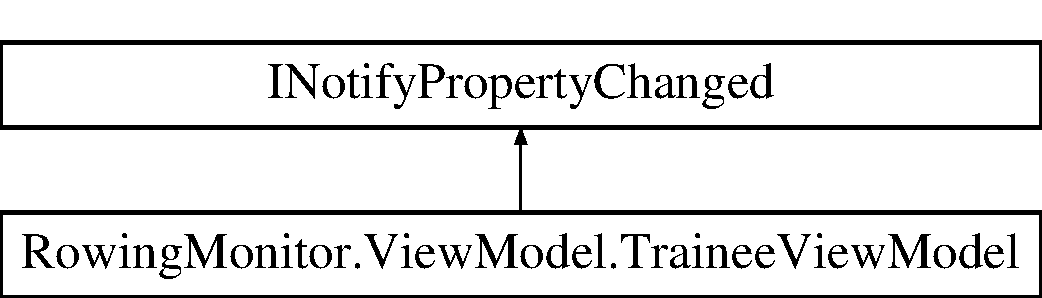
\includegraphics[height=2.000000cm]{class_rowing_monitor_1_1_view_model_1_1_trainee_view_model}
\end{center}
\end{figure}
\subsection*{Public Member Functions}
\begin{DoxyCompactItemize}
\item 
\hyperlink{class_rowing_monitor_1_1_view_model_1_1_trainee_view_model_a97f8f56fd0414366f18cf93c041ac107}{Trainee\+View\+Model} ()
\item 
void \hyperlink{class_rowing_monitor_1_1_view_model_1_1_trainee_view_model_a9ca701305abf7846b36efd285d0acc71}{View\+Loaded} ()
\item 
void \hyperlink{class_rowing_monitor_1_1_view_model_1_1_trainee_view_model_a404af3ee49d67f777876beae5b4397c1}{View\+Unloaded} ()
\end{DoxyCompactItemize}
\subsection*{Properties}
\begin{DoxyCompactItemize}
\item 
string \hyperlink{class_rowing_monitor_1_1_view_model_1_1_trainee_view_model_aeb6c056cdfa3855f42ae5954ea11f20d}{Session\+Time}\hspace{0.3cm}{\ttfamily  \mbox{[}get, set\mbox{]}}
\item 
string \hyperlink{class_rowing_monitor_1_1_view_model_1_1_trainee_view_model_a931c2a2c640cf7d42cfb29d1e21049af}{Stroke\+Count}\hspace{0.3cm}{\ttfamily  \mbox{[}get, set\mbox{]}}
\item 
string \hyperlink{class_rowing_monitor_1_1_view_model_1_1_trainee_view_model_ac4d37599e83e9a8a79f4f101d61c1223}{Stroke\+Rate}\hspace{0.3cm}{\ttfamily  \mbox{[}get, set\mbox{]}}
\item 
string \hyperlink{class_rowing_monitor_1_1_view_model_1_1_trainee_view_model_abeea8b0717e76fcb5bb300ba96f50b2b}{Mean\+Stroke\+Length}\hspace{0.3cm}{\ttfamily  \mbox{[}get, set\mbox{]}}
\item 
string \hyperlink{class_rowing_monitor_1_1_view_model_1_1_trainee_view_model_a3528ab6aaf531da1b58fbcb841bf6289}{Mean\+Seat\+Travel}\hspace{0.3cm}{\ttfamily  \mbox{[}get, set\mbox{]}}
\item 
string \hyperlink{class_rowing_monitor_1_1_view_model_1_1_trainee_view_model_a3b991710dd1abe5a0292242d84b751bb}{Mean\+Stroke\+Time}\hspace{0.3cm}{\ttfamily  \mbox{[}get, set\mbox{]}}
\item 
Grid \hyperlink{class_rowing_monitor_1_1_view_model_1_1_trainee_view_model_a4fab1e779e1336f06f79849e2128459d}{Main\+Grid}\hspace{0.3cm}{\ttfamily  \mbox{[}get, set\mbox{]}}
\end{DoxyCompactItemize}
\subsection*{Events}
\begin{DoxyCompactItemize}
\item 
Property\+Changed\+Event\+Handler \hyperlink{class_rowing_monitor_1_1_view_model_1_1_trainee_view_model_a33d6d8137f217e3c51d97e8f6b871ab8}{Property\+Changed}
\end{DoxyCompactItemize}


\subsection{Constructor \& Destructor Documentation}
\mbox{\Hypertarget{class_rowing_monitor_1_1_view_model_1_1_trainee_view_model_a97f8f56fd0414366f18cf93c041ac107}\label{class_rowing_monitor_1_1_view_model_1_1_trainee_view_model_a97f8f56fd0414366f18cf93c041ac107}} 
\index{Rowing\+Monitor\+::\+View\+Model\+::\+Trainee\+View\+Model@{Rowing\+Monitor\+::\+View\+Model\+::\+Trainee\+View\+Model}!Trainee\+View\+Model@{Trainee\+View\+Model}}
\index{Trainee\+View\+Model@{Trainee\+View\+Model}!Rowing\+Monitor\+::\+View\+Model\+::\+Trainee\+View\+Model@{Rowing\+Monitor\+::\+View\+Model\+::\+Trainee\+View\+Model}}
\subsubsection{\texorpdfstring{Trainee\+View\+Model()}{TraineeViewModel()}}
{\footnotesize\ttfamily Rowing\+Monitor.\+View\+Model.\+Trainee\+View\+Model.\+Trainee\+View\+Model (\begin{DoxyParamCaption}{ }\end{DoxyParamCaption})}



\subsection{Member Function Documentation}
\mbox{\Hypertarget{class_rowing_monitor_1_1_view_model_1_1_trainee_view_model_a9ca701305abf7846b36efd285d0acc71}\label{class_rowing_monitor_1_1_view_model_1_1_trainee_view_model_a9ca701305abf7846b36efd285d0acc71}} 
\index{Rowing\+Monitor\+::\+View\+Model\+::\+Trainee\+View\+Model@{Rowing\+Monitor\+::\+View\+Model\+::\+Trainee\+View\+Model}!View\+Loaded@{View\+Loaded}}
\index{View\+Loaded@{View\+Loaded}!Rowing\+Monitor\+::\+View\+Model\+::\+Trainee\+View\+Model@{Rowing\+Monitor\+::\+View\+Model\+::\+Trainee\+View\+Model}}
\subsubsection{\texorpdfstring{View\+Loaded()}{ViewLoaded()}}
{\footnotesize\ttfamily void Rowing\+Monitor.\+View\+Model.\+Trainee\+View\+Model.\+View\+Loaded (\begin{DoxyParamCaption}{ }\end{DoxyParamCaption})}

\mbox{\Hypertarget{class_rowing_monitor_1_1_view_model_1_1_trainee_view_model_a404af3ee49d67f777876beae5b4397c1}\label{class_rowing_monitor_1_1_view_model_1_1_trainee_view_model_a404af3ee49d67f777876beae5b4397c1}} 
\index{Rowing\+Monitor\+::\+View\+Model\+::\+Trainee\+View\+Model@{Rowing\+Monitor\+::\+View\+Model\+::\+Trainee\+View\+Model}!View\+Unloaded@{View\+Unloaded}}
\index{View\+Unloaded@{View\+Unloaded}!Rowing\+Monitor\+::\+View\+Model\+::\+Trainee\+View\+Model@{Rowing\+Monitor\+::\+View\+Model\+::\+Trainee\+View\+Model}}
\subsubsection{\texorpdfstring{View\+Unloaded()}{ViewUnloaded()}}
{\footnotesize\ttfamily void Rowing\+Monitor.\+View\+Model.\+Trainee\+View\+Model.\+View\+Unloaded (\begin{DoxyParamCaption}{ }\end{DoxyParamCaption})}



\subsection{Property Documentation}
\mbox{\Hypertarget{class_rowing_monitor_1_1_view_model_1_1_trainee_view_model_a4fab1e779e1336f06f79849e2128459d}\label{class_rowing_monitor_1_1_view_model_1_1_trainee_view_model_a4fab1e779e1336f06f79849e2128459d}} 
\index{Rowing\+Monitor\+::\+View\+Model\+::\+Trainee\+View\+Model@{Rowing\+Monitor\+::\+View\+Model\+::\+Trainee\+View\+Model}!Main\+Grid@{Main\+Grid}}
\index{Main\+Grid@{Main\+Grid}!Rowing\+Monitor\+::\+View\+Model\+::\+Trainee\+View\+Model@{Rowing\+Monitor\+::\+View\+Model\+::\+Trainee\+View\+Model}}
\subsubsection{\texorpdfstring{Main\+Grid}{MainGrid}}
{\footnotesize\ttfamily Grid Rowing\+Monitor.\+View\+Model.\+Trainee\+View\+Model.\+Main\+Grid\hspace{0.3cm}{\ttfamily [get]}, {\ttfamily [set]}}

\mbox{\Hypertarget{class_rowing_monitor_1_1_view_model_1_1_trainee_view_model_a3528ab6aaf531da1b58fbcb841bf6289}\label{class_rowing_monitor_1_1_view_model_1_1_trainee_view_model_a3528ab6aaf531da1b58fbcb841bf6289}} 
\index{Rowing\+Monitor\+::\+View\+Model\+::\+Trainee\+View\+Model@{Rowing\+Monitor\+::\+View\+Model\+::\+Trainee\+View\+Model}!Mean\+Seat\+Travel@{Mean\+Seat\+Travel}}
\index{Mean\+Seat\+Travel@{Mean\+Seat\+Travel}!Rowing\+Monitor\+::\+View\+Model\+::\+Trainee\+View\+Model@{Rowing\+Monitor\+::\+View\+Model\+::\+Trainee\+View\+Model}}
\subsubsection{\texorpdfstring{Mean\+Seat\+Travel}{MeanSeatTravel}}
{\footnotesize\ttfamily string Rowing\+Monitor.\+View\+Model.\+Trainee\+View\+Model.\+Mean\+Seat\+Travel\hspace{0.3cm}{\ttfamily [get]}, {\ttfamily [set]}}

\mbox{\Hypertarget{class_rowing_monitor_1_1_view_model_1_1_trainee_view_model_abeea8b0717e76fcb5bb300ba96f50b2b}\label{class_rowing_monitor_1_1_view_model_1_1_trainee_view_model_abeea8b0717e76fcb5bb300ba96f50b2b}} 
\index{Rowing\+Monitor\+::\+View\+Model\+::\+Trainee\+View\+Model@{Rowing\+Monitor\+::\+View\+Model\+::\+Trainee\+View\+Model}!Mean\+Stroke\+Length@{Mean\+Stroke\+Length}}
\index{Mean\+Stroke\+Length@{Mean\+Stroke\+Length}!Rowing\+Monitor\+::\+View\+Model\+::\+Trainee\+View\+Model@{Rowing\+Monitor\+::\+View\+Model\+::\+Trainee\+View\+Model}}
\subsubsection{\texorpdfstring{Mean\+Stroke\+Length}{MeanStrokeLength}}
{\footnotesize\ttfamily string Rowing\+Monitor.\+View\+Model.\+Trainee\+View\+Model.\+Mean\+Stroke\+Length\hspace{0.3cm}{\ttfamily [get]}, {\ttfamily [set]}}

\mbox{\Hypertarget{class_rowing_monitor_1_1_view_model_1_1_trainee_view_model_a3b991710dd1abe5a0292242d84b751bb}\label{class_rowing_monitor_1_1_view_model_1_1_trainee_view_model_a3b991710dd1abe5a0292242d84b751bb}} 
\index{Rowing\+Monitor\+::\+View\+Model\+::\+Trainee\+View\+Model@{Rowing\+Monitor\+::\+View\+Model\+::\+Trainee\+View\+Model}!Mean\+Stroke\+Time@{Mean\+Stroke\+Time}}
\index{Mean\+Stroke\+Time@{Mean\+Stroke\+Time}!Rowing\+Monitor\+::\+View\+Model\+::\+Trainee\+View\+Model@{Rowing\+Monitor\+::\+View\+Model\+::\+Trainee\+View\+Model}}
\subsubsection{\texorpdfstring{Mean\+Stroke\+Time}{MeanStrokeTime}}
{\footnotesize\ttfamily string Rowing\+Monitor.\+View\+Model.\+Trainee\+View\+Model.\+Mean\+Stroke\+Time\hspace{0.3cm}{\ttfamily [get]}, {\ttfamily [set]}}

\mbox{\Hypertarget{class_rowing_monitor_1_1_view_model_1_1_trainee_view_model_aeb6c056cdfa3855f42ae5954ea11f20d}\label{class_rowing_monitor_1_1_view_model_1_1_trainee_view_model_aeb6c056cdfa3855f42ae5954ea11f20d}} 
\index{Rowing\+Monitor\+::\+View\+Model\+::\+Trainee\+View\+Model@{Rowing\+Monitor\+::\+View\+Model\+::\+Trainee\+View\+Model}!Session\+Time@{Session\+Time}}
\index{Session\+Time@{Session\+Time}!Rowing\+Monitor\+::\+View\+Model\+::\+Trainee\+View\+Model@{Rowing\+Monitor\+::\+View\+Model\+::\+Trainee\+View\+Model}}
\subsubsection{\texorpdfstring{Session\+Time}{SessionTime}}
{\footnotesize\ttfamily string Rowing\+Monitor.\+View\+Model.\+Trainee\+View\+Model.\+Session\+Time\hspace{0.3cm}{\ttfamily [get]}, {\ttfamily [set]}}

\mbox{\Hypertarget{class_rowing_monitor_1_1_view_model_1_1_trainee_view_model_a931c2a2c640cf7d42cfb29d1e21049af}\label{class_rowing_monitor_1_1_view_model_1_1_trainee_view_model_a931c2a2c640cf7d42cfb29d1e21049af}} 
\index{Rowing\+Monitor\+::\+View\+Model\+::\+Trainee\+View\+Model@{Rowing\+Monitor\+::\+View\+Model\+::\+Trainee\+View\+Model}!Stroke\+Count@{Stroke\+Count}}
\index{Stroke\+Count@{Stroke\+Count}!Rowing\+Monitor\+::\+View\+Model\+::\+Trainee\+View\+Model@{Rowing\+Monitor\+::\+View\+Model\+::\+Trainee\+View\+Model}}
\subsubsection{\texorpdfstring{Stroke\+Count}{StrokeCount}}
{\footnotesize\ttfamily string Rowing\+Monitor.\+View\+Model.\+Trainee\+View\+Model.\+Stroke\+Count\hspace{0.3cm}{\ttfamily [get]}, {\ttfamily [set]}}

\mbox{\Hypertarget{class_rowing_monitor_1_1_view_model_1_1_trainee_view_model_ac4d37599e83e9a8a79f4f101d61c1223}\label{class_rowing_monitor_1_1_view_model_1_1_trainee_view_model_ac4d37599e83e9a8a79f4f101d61c1223}} 
\index{Rowing\+Monitor\+::\+View\+Model\+::\+Trainee\+View\+Model@{Rowing\+Monitor\+::\+View\+Model\+::\+Trainee\+View\+Model}!Stroke\+Rate@{Stroke\+Rate}}
\index{Stroke\+Rate@{Stroke\+Rate}!Rowing\+Monitor\+::\+View\+Model\+::\+Trainee\+View\+Model@{Rowing\+Monitor\+::\+View\+Model\+::\+Trainee\+View\+Model}}
\subsubsection{\texorpdfstring{Stroke\+Rate}{StrokeRate}}
{\footnotesize\ttfamily string Rowing\+Monitor.\+View\+Model.\+Trainee\+View\+Model.\+Stroke\+Rate\hspace{0.3cm}{\ttfamily [get]}, {\ttfamily [set]}}



\subsection{Event Documentation}
\mbox{\Hypertarget{class_rowing_monitor_1_1_view_model_1_1_trainee_view_model_a33d6d8137f217e3c51d97e8f6b871ab8}\label{class_rowing_monitor_1_1_view_model_1_1_trainee_view_model_a33d6d8137f217e3c51d97e8f6b871ab8}} 
\index{Rowing\+Monitor\+::\+View\+Model\+::\+Trainee\+View\+Model@{Rowing\+Monitor\+::\+View\+Model\+::\+Trainee\+View\+Model}!Property\+Changed@{Property\+Changed}}
\index{Property\+Changed@{Property\+Changed}!Rowing\+Monitor\+::\+View\+Model\+::\+Trainee\+View\+Model@{Rowing\+Monitor\+::\+View\+Model\+::\+Trainee\+View\+Model}}
\subsubsection{\texorpdfstring{Property\+Changed}{PropertyChanged}}
{\footnotesize\ttfamily Property\+Changed\+Event\+Handler Rowing\+Monitor.\+View\+Model.\+Trainee\+View\+Model.\+Property\+Changed}



The documentation for this class was generated from the following file\+:\begin{DoxyCompactItemize}
\item 
View\+Model/\hyperlink{_trainee_view_model_8cs}{Trainee\+View\+Model.\+cs}\end{DoxyCompactItemize}

\hypertarget{struct_rowing_monitor_1_1_model_1_1_pipeline_1_1_kinect_joint_smoothing_filter_1_1_t_r_a_n_s_f_o9fb8ee9e37e15ee7ab8d318a72b8984e}{}\section{Rowing\+Monitor.\+Model.\+Pipeline.\+Kinect\+Joint\+Smoothing\+Filter.\+T\+R\+A\+N\+S\+F\+O\+R\+M\+\_\+\+S\+M\+O\+O\+T\+H\+\_\+\+P\+A\+R\+A\+M\+E\+T\+E\+RS Struct Reference}
\label{struct_rowing_monitor_1_1_model_1_1_pipeline_1_1_kinect_joint_smoothing_filter_1_1_t_r_a_n_s_f_o9fb8ee9e37e15ee7ab8d318a72b8984e}\index{Rowing\+Monitor.\+Model.\+Pipeline.\+Kinect\+Joint\+Smoothing\+Filter.\+T\+R\+A\+N\+S\+F\+O\+R\+M\+\_\+\+S\+M\+O\+O\+T\+H\+\_\+\+P\+A\+R\+A\+M\+E\+T\+E\+RS@{Rowing\+Monitor.\+Model.\+Pipeline.\+Kinect\+Joint\+Smoothing\+Filter.\+T\+R\+A\+N\+S\+F\+O\+R\+M\+\_\+\+S\+M\+O\+O\+T\+H\+\_\+\+P\+A\+R\+A\+M\+E\+T\+E\+RS}}
\subsection*{Public Attributes}
\begin{DoxyCompactItemize}
\item 
float \hyperlink{struct_rowing_monitor_1_1_model_1_1_pipeline_1_1_kinect_joint_smoothing_filter_1_1_t_r_a_n_s_f_o9fb8ee9e37e15ee7ab8d318a72b8984e_a5fd02a9b999cbcc12ad1a22763adb8cd}{f\+Smoothing}
\item 
float \hyperlink{struct_rowing_monitor_1_1_model_1_1_pipeline_1_1_kinect_joint_smoothing_filter_1_1_t_r_a_n_s_f_o9fb8ee9e37e15ee7ab8d318a72b8984e_a7303c0fbcd8a80670f7ddd5f46c0d49c}{f\+Correction}
\item 
float \hyperlink{struct_rowing_monitor_1_1_model_1_1_pipeline_1_1_kinect_joint_smoothing_filter_1_1_t_r_a_n_s_f_o9fb8ee9e37e15ee7ab8d318a72b8984e_a4cc3828d097b5b63f71f004f2034ba79}{f\+Prediction}
\item 
float \hyperlink{struct_rowing_monitor_1_1_model_1_1_pipeline_1_1_kinect_joint_smoothing_filter_1_1_t_r_a_n_s_f_o9fb8ee9e37e15ee7ab8d318a72b8984e_aa4a54259125f5677ef2b7a149402e268}{f\+Jitter\+Radius}
\item 
float \hyperlink{struct_rowing_monitor_1_1_model_1_1_pipeline_1_1_kinect_joint_smoothing_filter_1_1_t_r_a_n_s_f_o9fb8ee9e37e15ee7ab8d318a72b8984e_a01f36a8e40cd63c55161e3df85de9196}{f\+Max\+Deviation\+Radius}
\end{DoxyCompactItemize}


\subsection{Member Data Documentation}
\mbox{\Hypertarget{struct_rowing_monitor_1_1_model_1_1_pipeline_1_1_kinect_joint_smoothing_filter_1_1_t_r_a_n_s_f_o9fb8ee9e37e15ee7ab8d318a72b8984e_a7303c0fbcd8a80670f7ddd5f46c0d49c}\label{struct_rowing_monitor_1_1_model_1_1_pipeline_1_1_kinect_joint_smoothing_filter_1_1_t_r_a_n_s_f_o9fb8ee9e37e15ee7ab8d318a72b8984e_a7303c0fbcd8a80670f7ddd5f46c0d49c}} 
\index{Rowing\+Monitor\+::\+Model\+::\+Pipeline\+::\+Kinect\+Joint\+Smoothing\+Filter\+::\+T\+R\+A\+N\+S\+F\+O\+R\+M\+\_\+\+S\+M\+O\+O\+T\+H\+\_\+\+P\+A\+R\+A\+M\+E\+T\+E\+RS@{Rowing\+Monitor\+::\+Model\+::\+Pipeline\+::\+Kinect\+Joint\+Smoothing\+Filter\+::\+T\+R\+A\+N\+S\+F\+O\+R\+M\+\_\+\+S\+M\+O\+O\+T\+H\+\_\+\+P\+A\+R\+A\+M\+E\+T\+E\+RS}!f\+Correction@{f\+Correction}}
\index{f\+Correction@{f\+Correction}!Rowing\+Monitor\+::\+Model\+::\+Pipeline\+::\+Kinect\+Joint\+Smoothing\+Filter\+::\+T\+R\+A\+N\+S\+F\+O\+R\+M\+\_\+\+S\+M\+O\+O\+T\+H\+\_\+\+P\+A\+R\+A\+M\+E\+T\+E\+RS@{Rowing\+Monitor\+::\+Model\+::\+Pipeline\+::\+Kinect\+Joint\+Smoothing\+Filter\+::\+T\+R\+A\+N\+S\+F\+O\+R\+M\+\_\+\+S\+M\+O\+O\+T\+H\+\_\+\+P\+A\+R\+A\+M\+E\+T\+E\+RS}}
\subsubsection{\texorpdfstring{f\+Correction}{fCorrection}}
{\footnotesize\ttfamily float Rowing\+Monitor.\+Model.\+Pipeline.\+Kinect\+Joint\+Smoothing\+Filter.\+T\+R\+A\+N\+S\+F\+O\+R\+M\+\_\+\+S\+M\+O\+O\+T\+H\+\_\+\+P\+A\+R\+A\+M\+E\+T\+E\+R\+S.\+f\+Correction}

\mbox{\Hypertarget{struct_rowing_monitor_1_1_model_1_1_pipeline_1_1_kinect_joint_smoothing_filter_1_1_t_r_a_n_s_f_o9fb8ee9e37e15ee7ab8d318a72b8984e_aa4a54259125f5677ef2b7a149402e268}\label{struct_rowing_monitor_1_1_model_1_1_pipeline_1_1_kinect_joint_smoothing_filter_1_1_t_r_a_n_s_f_o9fb8ee9e37e15ee7ab8d318a72b8984e_aa4a54259125f5677ef2b7a149402e268}} 
\index{Rowing\+Monitor\+::\+Model\+::\+Pipeline\+::\+Kinect\+Joint\+Smoothing\+Filter\+::\+T\+R\+A\+N\+S\+F\+O\+R\+M\+\_\+\+S\+M\+O\+O\+T\+H\+\_\+\+P\+A\+R\+A\+M\+E\+T\+E\+RS@{Rowing\+Monitor\+::\+Model\+::\+Pipeline\+::\+Kinect\+Joint\+Smoothing\+Filter\+::\+T\+R\+A\+N\+S\+F\+O\+R\+M\+\_\+\+S\+M\+O\+O\+T\+H\+\_\+\+P\+A\+R\+A\+M\+E\+T\+E\+RS}!f\+Jitter\+Radius@{f\+Jitter\+Radius}}
\index{f\+Jitter\+Radius@{f\+Jitter\+Radius}!Rowing\+Monitor\+::\+Model\+::\+Pipeline\+::\+Kinect\+Joint\+Smoothing\+Filter\+::\+T\+R\+A\+N\+S\+F\+O\+R\+M\+\_\+\+S\+M\+O\+O\+T\+H\+\_\+\+P\+A\+R\+A\+M\+E\+T\+E\+RS@{Rowing\+Monitor\+::\+Model\+::\+Pipeline\+::\+Kinect\+Joint\+Smoothing\+Filter\+::\+T\+R\+A\+N\+S\+F\+O\+R\+M\+\_\+\+S\+M\+O\+O\+T\+H\+\_\+\+P\+A\+R\+A\+M\+E\+T\+E\+RS}}
\subsubsection{\texorpdfstring{f\+Jitter\+Radius}{fJitterRadius}}
{\footnotesize\ttfamily float Rowing\+Monitor.\+Model.\+Pipeline.\+Kinect\+Joint\+Smoothing\+Filter.\+T\+R\+A\+N\+S\+F\+O\+R\+M\+\_\+\+S\+M\+O\+O\+T\+H\+\_\+\+P\+A\+R\+A\+M\+E\+T\+E\+R\+S.\+f\+Jitter\+Radius}

\mbox{\Hypertarget{struct_rowing_monitor_1_1_model_1_1_pipeline_1_1_kinect_joint_smoothing_filter_1_1_t_r_a_n_s_f_o9fb8ee9e37e15ee7ab8d318a72b8984e_a01f36a8e40cd63c55161e3df85de9196}\label{struct_rowing_monitor_1_1_model_1_1_pipeline_1_1_kinect_joint_smoothing_filter_1_1_t_r_a_n_s_f_o9fb8ee9e37e15ee7ab8d318a72b8984e_a01f36a8e40cd63c55161e3df85de9196}} 
\index{Rowing\+Monitor\+::\+Model\+::\+Pipeline\+::\+Kinect\+Joint\+Smoothing\+Filter\+::\+T\+R\+A\+N\+S\+F\+O\+R\+M\+\_\+\+S\+M\+O\+O\+T\+H\+\_\+\+P\+A\+R\+A\+M\+E\+T\+E\+RS@{Rowing\+Monitor\+::\+Model\+::\+Pipeline\+::\+Kinect\+Joint\+Smoothing\+Filter\+::\+T\+R\+A\+N\+S\+F\+O\+R\+M\+\_\+\+S\+M\+O\+O\+T\+H\+\_\+\+P\+A\+R\+A\+M\+E\+T\+E\+RS}!f\+Max\+Deviation\+Radius@{f\+Max\+Deviation\+Radius}}
\index{f\+Max\+Deviation\+Radius@{f\+Max\+Deviation\+Radius}!Rowing\+Monitor\+::\+Model\+::\+Pipeline\+::\+Kinect\+Joint\+Smoothing\+Filter\+::\+T\+R\+A\+N\+S\+F\+O\+R\+M\+\_\+\+S\+M\+O\+O\+T\+H\+\_\+\+P\+A\+R\+A\+M\+E\+T\+E\+RS@{Rowing\+Monitor\+::\+Model\+::\+Pipeline\+::\+Kinect\+Joint\+Smoothing\+Filter\+::\+T\+R\+A\+N\+S\+F\+O\+R\+M\+\_\+\+S\+M\+O\+O\+T\+H\+\_\+\+P\+A\+R\+A\+M\+E\+T\+E\+RS}}
\subsubsection{\texorpdfstring{f\+Max\+Deviation\+Radius}{fMaxDeviationRadius}}
{\footnotesize\ttfamily float Rowing\+Monitor.\+Model.\+Pipeline.\+Kinect\+Joint\+Smoothing\+Filter.\+T\+R\+A\+N\+S\+F\+O\+R\+M\+\_\+\+S\+M\+O\+O\+T\+H\+\_\+\+P\+A\+R\+A\+M\+E\+T\+E\+R\+S.\+f\+Max\+Deviation\+Radius}

\mbox{\Hypertarget{struct_rowing_monitor_1_1_model_1_1_pipeline_1_1_kinect_joint_smoothing_filter_1_1_t_r_a_n_s_f_o9fb8ee9e37e15ee7ab8d318a72b8984e_a4cc3828d097b5b63f71f004f2034ba79}\label{struct_rowing_monitor_1_1_model_1_1_pipeline_1_1_kinect_joint_smoothing_filter_1_1_t_r_a_n_s_f_o9fb8ee9e37e15ee7ab8d318a72b8984e_a4cc3828d097b5b63f71f004f2034ba79}} 
\index{Rowing\+Monitor\+::\+Model\+::\+Pipeline\+::\+Kinect\+Joint\+Smoothing\+Filter\+::\+T\+R\+A\+N\+S\+F\+O\+R\+M\+\_\+\+S\+M\+O\+O\+T\+H\+\_\+\+P\+A\+R\+A\+M\+E\+T\+E\+RS@{Rowing\+Monitor\+::\+Model\+::\+Pipeline\+::\+Kinect\+Joint\+Smoothing\+Filter\+::\+T\+R\+A\+N\+S\+F\+O\+R\+M\+\_\+\+S\+M\+O\+O\+T\+H\+\_\+\+P\+A\+R\+A\+M\+E\+T\+E\+RS}!f\+Prediction@{f\+Prediction}}
\index{f\+Prediction@{f\+Prediction}!Rowing\+Monitor\+::\+Model\+::\+Pipeline\+::\+Kinect\+Joint\+Smoothing\+Filter\+::\+T\+R\+A\+N\+S\+F\+O\+R\+M\+\_\+\+S\+M\+O\+O\+T\+H\+\_\+\+P\+A\+R\+A\+M\+E\+T\+E\+RS@{Rowing\+Monitor\+::\+Model\+::\+Pipeline\+::\+Kinect\+Joint\+Smoothing\+Filter\+::\+T\+R\+A\+N\+S\+F\+O\+R\+M\+\_\+\+S\+M\+O\+O\+T\+H\+\_\+\+P\+A\+R\+A\+M\+E\+T\+E\+RS}}
\subsubsection{\texorpdfstring{f\+Prediction}{fPrediction}}
{\footnotesize\ttfamily float Rowing\+Monitor.\+Model.\+Pipeline.\+Kinect\+Joint\+Smoothing\+Filter.\+T\+R\+A\+N\+S\+F\+O\+R\+M\+\_\+\+S\+M\+O\+O\+T\+H\+\_\+\+P\+A\+R\+A\+M\+E\+T\+E\+R\+S.\+f\+Prediction}

\mbox{\Hypertarget{struct_rowing_monitor_1_1_model_1_1_pipeline_1_1_kinect_joint_smoothing_filter_1_1_t_r_a_n_s_f_o9fb8ee9e37e15ee7ab8d318a72b8984e_a5fd02a9b999cbcc12ad1a22763adb8cd}\label{struct_rowing_monitor_1_1_model_1_1_pipeline_1_1_kinect_joint_smoothing_filter_1_1_t_r_a_n_s_f_o9fb8ee9e37e15ee7ab8d318a72b8984e_a5fd02a9b999cbcc12ad1a22763adb8cd}} 
\index{Rowing\+Monitor\+::\+Model\+::\+Pipeline\+::\+Kinect\+Joint\+Smoothing\+Filter\+::\+T\+R\+A\+N\+S\+F\+O\+R\+M\+\_\+\+S\+M\+O\+O\+T\+H\+\_\+\+P\+A\+R\+A\+M\+E\+T\+E\+RS@{Rowing\+Monitor\+::\+Model\+::\+Pipeline\+::\+Kinect\+Joint\+Smoothing\+Filter\+::\+T\+R\+A\+N\+S\+F\+O\+R\+M\+\_\+\+S\+M\+O\+O\+T\+H\+\_\+\+P\+A\+R\+A\+M\+E\+T\+E\+RS}!f\+Smoothing@{f\+Smoothing}}
\index{f\+Smoothing@{f\+Smoothing}!Rowing\+Monitor\+::\+Model\+::\+Pipeline\+::\+Kinect\+Joint\+Smoothing\+Filter\+::\+T\+R\+A\+N\+S\+F\+O\+R\+M\+\_\+\+S\+M\+O\+O\+T\+H\+\_\+\+P\+A\+R\+A\+M\+E\+T\+E\+RS@{Rowing\+Monitor\+::\+Model\+::\+Pipeline\+::\+Kinect\+Joint\+Smoothing\+Filter\+::\+T\+R\+A\+N\+S\+F\+O\+R\+M\+\_\+\+S\+M\+O\+O\+T\+H\+\_\+\+P\+A\+R\+A\+M\+E\+T\+E\+RS}}
\subsubsection{\texorpdfstring{f\+Smoothing}{fSmoothing}}
{\footnotesize\ttfamily float Rowing\+Monitor.\+Model.\+Pipeline.\+Kinect\+Joint\+Smoothing\+Filter.\+T\+R\+A\+N\+S\+F\+O\+R\+M\+\_\+\+S\+M\+O\+O\+T\+H\+\_\+\+P\+A\+R\+A\+M\+E\+T\+E\+R\+S.\+f\+Smoothing}



The documentation for this struct was generated from the following file\+:\begin{DoxyCompactItemize}
\item 
Model/\+Pipeline/\hyperlink{_kinect_joint_smoothing_filter_8cs}{Kinect\+Joint\+Smoothing\+Filter.\+cs}\end{DoxyCompactItemize}

\hypertarget{class_rowing_monitor_1_1_model_1_1_pipeline_1_1_trunk_angle_display}{}\section{Rowing\+Monitor.\+Model.\+Pipeline.\+Trunk\+Angle\+Display Class Reference}
\label{class_rowing_monitor_1_1_model_1_1_pipeline_1_1_trunk_angle_display}\index{Rowing\+Monitor.\+Model.\+Pipeline.\+Trunk\+Angle\+Display@{Rowing\+Monitor.\+Model.\+Pipeline.\+Trunk\+Angle\+Display}}
\subsection*{Public Member Functions}
\begin{DoxyCompactItemize}
\item 
\hyperlink{class_rowing_monitor_1_1_model_1_1_pipeline_1_1_trunk_angle_display_aa821fa5b4473ec7cc3ce2947fb9b4b73}{Trunk\+Angle\+Display} ()
\item 
void \hyperlink{class_rowing_monitor_1_1_model_1_1_pipeline_1_1_trunk_angle_display_a3f82a22f8d195e8285ec1008514b8a3a}{Render} ()
\end{DoxyCompactItemize}
\subsection*{Properties}
\begin{DoxyCompactItemize}
\item 
Action\+Block$<$ \hyperlink{struct_rowing_monitor_1_1_model_1_1_util_1_1_joint_data}{Joint\+Data} $>$ \hyperlink{class_rowing_monitor_1_1_model_1_1_pipeline_1_1_trunk_angle_display_a2bbac9839cfa5977f133be79c3c47754}{Input}\hspace{0.3cm}{\ttfamily  \mbox{[}get, set\mbox{]}}
\item 
\hyperlink{class_rowing_monitor_1_1_view_1_1_trunk_angle_view}{Trunk\+Angle\+View} \hyperlink{class_rowing_monitor_1_1_model_1_1_pipeline_1_1_trunk_angle_display_ac0578beabcf4ec767137c3e7b9d50493}{View}\hspace{0.3cm}{\ttfamily  \mbox{[}get, set\mbox{]}}
\end{DoxyCompactItemize}


\subsection{Constructor \& Destructor Documentation}
\mbox{\Hypertarget{class_rowing_monitor_1_1_model_1_1_pipeline_1_1_trunk_angle_display_aa821fa5b4473ec7cc3ce2947fb9b4b73}\label{class_rowing_monitor_1_1_model_1_1_pipeline_1_1_trunk_angle_display_aa821fa5b4473ec7cc3ce2947fb9b4b73}} 
\index{Rowing\+Monitor\+::\+Model\+::\+Pipeline\+::\+Trunk\+Angle\+Display@{Rowing\+Monitor\+::\+Model\+::\+Pipeline\+::\+Trunk\+Angle\+Display}!Trunk\+Angle\+Display@{Trunk\+Angle\+Display}}
\index{Trunk\+Angle\+Display@{Trunk\+Angle\+Display}!Rowing\+Monitor\+::\+Model\+::\+Pipeline\+::\+Trunk\+Angle\+Display@{Rowing\+Monitor\+::\+Model\+::\+Pipeline\+::\+Trunk\+Angle\+Display}}
\subsubsection{\texorpdfstring{Trunk\+Angle\+Display()}{TrunkAngleDisplay()}}
{\footnotesize\ttfamily Rowing\+Monitor.\+Model.\+Pipeline.\+Trunk\+Angle\+Display.\+Trunk\+Angle\+Display (\begin{DoxyParamCaption}{ }\end{DoxyParamCaption})}



\subsection{Member Function Documentation}
\mbox{\Hypertarget{class_rowing_monitor_1_1_model_1_1_pipeline_1_1_trunk_angle_display_a3f82a22f8d195e8285ec1008514b8a3a}\label{class_rowing_monitor_1_1_model_1_1_pipeline_1_1_trunk_angle_display_a3f82a22f8d195e8285ec1008514b8a3a}} 
\index{Rowing\+Monitor\+::\+Model\+::\+Pipeline\+::\+Trunk\+Angle\+Display@{Rowing\+Monitor\+::\+Model\+::\+Pipeline\+::\+Trunk\+Angle\+Display}!Render@{Render}}
\index{Render@{Render}!Rowing\+Monitor\+::\+Model\+::\+Pipeline\+::\+Trunk\+Angle\+Display@{Rowing\+Monitor\+::\+Model\+::\+Pipeline\+::\+Trunk\+Angle\+Display}}
\subsubsection{\texorpdfstring{Render()}{Render()}}
{\footnotesize\ttfamily void Rowing\+Monitor.\+Model.\+Pipeline.\+Trunk\+Angle\+Display.\+Render (\begin{DoxyParamCaption}{ }\end{DoxyParamCaption})}



\subsection{Property Documentation}
\mbox{\Hypertarget{class_rowing_monitor_1_1_model_1_1_pipeline_1_1_trunk_angle_display_a2bbac9839cfa5977f133be79c3c47754}\label{class_rowing_monitor_1_1_model_1_1_pipeline_1_1_trunk_angle_display_a2bbac9839cfa5977f133be79c3c47754}} 
\index{Rowing\+Monitor\+::\+Model\+::\+Pipeline\+::\+Trunk\+Angle\+Display@{Rowing\+Monitor\+::\+Model\+::\+Pipeline\+::\+Trunk\+Angle\+Display}!Input@{Input}}
\index{Input@{Input}!Rowing\+Monitor\+::\+Model\+::\+Pipeline\+::\+Trunk\+Angle\+Display@{Rowing\+Monitor\+::\+Model\+::\+Pipeline\+::\+Trunk\+Angle\+Display}}
\subsubsection{\texorpdfstring{Input}{Input}}
{\footnotesize\ttfamily Action\+Block$<$\hyperlink{struct_rowing_monitor_1_1_model_1_1_util_1_1_joint_data}{Joint\+Data}$>$ Rowing\+Monitor.\+Model.\+Pipeline.\+Trunk\+Angle\+Display.\+Input\hspace{0.3cm}{\ttfamily [get]}, {\ttfamily [set]}}

\mbox{\Hypertarget{class_rowing_monitor_1_1_model_1_1_pipeline_1_1_trunk_angle_display_ac0578beabcf4ec767137c3e7b9d50493}\label{class_rowing_monitor_1_1_model_1_1_pipeline_1_1_trunk_angle_display_ac0578beabcf4ec767137c3e7b9d50493}} 
\index{Rowing\+Monitor\+::\+Model\+::\+Pipeline\+::\+Trunk\+Angle\+Display@{Rowing\+Monitor\+::\+Model\+::\+Pipeline\+::\+Trunk\+Angle\+Display}!View@{View}}
\index{View@{View}!Rowing\+Monitor\+::\+Model\+::\+Pipeline\+::\+Trunk\+Angle\+Display@{Rowing\+Monitor\+::\+Model\+::\+Pipeline\+::\+Trunk\+Angle\+Display}}
\subsubsection{\texorpdfstring{View}{View}}
{\footnotesize\ttfamily \hyperlink{class_rowing_monitor_1_1_view_1_1_trunk_angle_view}{Trunk\+Angle\+View} Rowing\+Monitor.\+Model.\+Pipeline.\+Trunk\+Angle\+Display.\+View\hspace{0.3cm}{\ttfamily [get]}, {\ttfamily [set]}}



The documentation for this class was generated from the following file\+:\begin{DoxyCompactItemize}
\item 
Model/\+Pipeline/\hyperlink{_trunk_angle_display_8cs}{Trunk\+Angle\+Display.\+cs}\end{DoxyCompactItemize}

\hypertarget{class_rowing_monitor_1_1_view_1_1_trunk_angle_view}{}\section{Rowing\+Monitor.\+View.\+Trunk\+Angle\+View Class Reference}
\label{class_rowing_monitor_1_1_view_1_1_trunk_angle_view}\index{Rowing\+Monitor.\+View.\+Trunk\+Angle\+View@{Rowing\+Monitor.\+View.\+Trunk\+Angle\+View}}


\hyperlink{class_rowing_monitor_1_1_view_1_1_trunk_angle_view}{Trunk\+Angle\+View}  


Inheritance diagram for Rowing\+Monitor.\+View.\+Trunk\+Angle\+View\+:\begin{figure}[H]
\begin{center}
\leavevmode
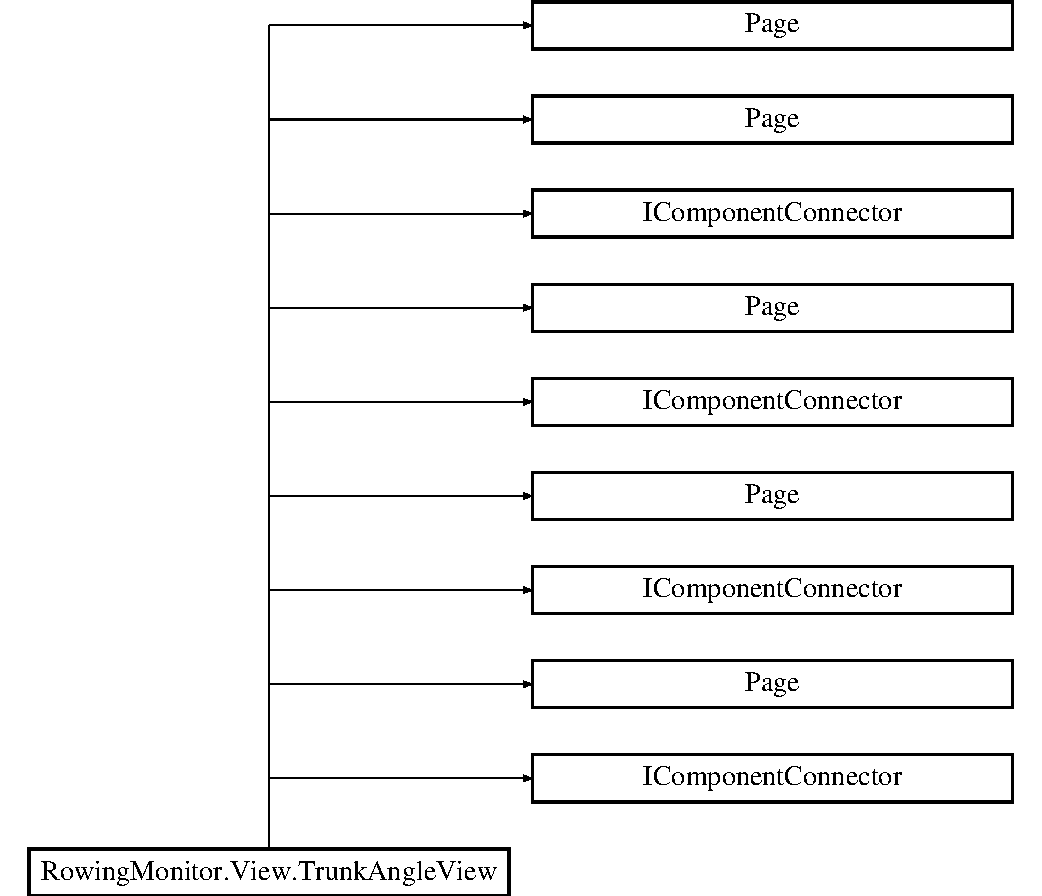
\includegraphics[height=10.000000cm]{class_rowing_monitor_1_1_view_1_1_trunk_angle_view}
\end{center}
\end{figure}
\subsection*{Public Member Functions}
\begin{DoxyCompactItemize}
\item 
void \hyperlink{class_rowing_monitor_1_1_view_1_1_trunk_angle_view_a0bb4fedfe9f2b058a0ee1ae5841242ce}{Initialize\+Component} ()
\begin{DoxyCompactList}\small\item\em Initialize\+Component \end{DoxyCompactList}\item 
void \hyperlink{class_rowing_monitor_1_1_view_1_1_trunk_angle_view_a0bb4fedfe9f2b058a0ee1ae5841242ce}{Initialize\+Component} ()
\begin{DoxyCompactList}\small\item\em Initialize\+Component \end{DoxyCompactList}\item 
void \hyperlink{class_rowing_monitor_1_1_view_1_1_trunk_angle_view_a0bb4fedfe9f2b058a0ee1ae5841242ce}{Initialize\+Component} ()
\begin{DoxyCompactList}\small\item\em Initialize\+Component \end{DoxyCompactList}\item 
void \hyperlink{class_rowing_monitor_1_1_view_1_1_trunk_angle_view_a0bb4fedfe9f2b058a0ee1ae5841242ce}{Initialize\+Component} ()
\begin{DoxyCompactList}\small\item\em Initialize\+Component \end{DoxyCompactList}\item 
\hyperlink{class_rowing_monitor_1_1_view_1_1_trunk_angle_view_a4a7e7129a25cf8a329e1b0744594f436}{Trunk\+Angle\+View} ()
\end{DoxyCompactItemize}


\subsection{Detailed Description}
\hyperlink{class_rowing_monitor_1_1_view_1_1_trunk_angle_view}{Trunk\+Angle\+View} 

Interaktionslogik für Trunk\+Angle\+View.\+xaml 

\subsection{Constructor \& Destructor Documentation}
\mbox{\Hypertarget{class_rowing_monitor_1_1_view_1_1_trunk_angle_view_a4a7e7129a25cf8a329e1b0744594f436}\label{class_rowing_monitor_1_1_view_1_1_trunk_angle_view_a4a7e7129a25cf8a329e1b0744594f436}} 
\index{Rowing\+Monitor\+::\+View\+::\+Trunk\+Angle\+View@{Rowing\+Monitor\+::\+View\+::\+Trunk\+Angle\+View}!Trunk\+Angle\+View@{Trunk\+Angle\+View}}
\index{Trunk\+Angle\+View@{Trunk\+Angle\+View}!Rowing\+Monitor\+::\+View\+::\+Trunk\+Angle\+View@{Rowing\+Monitor\+::\+View\+::\+Trunk\+Angle\+View}}
\subsubsection{\texorpdfstring{Trunk\+Angle\+View()}{TrunkAngleView()}}
{\footnotesize\ttfamily Rowing\+Monitor.\+View.\+Trunk\+Angle\+View.\+Trunk\+Angle\+View (\begin{DoxyParamCaption}{ }\end{DoxyParamCaption})}



\subsection{Member Function Documentation}
\mbox{\Hypertarget{class_rowing_monitor_1_1_view_1_1_trunk_angle_view_a0bb4fedfe9f2b058a0ee1ae5841242ce}\label{class_rowing_monitor_1_1_view_1_1_trunk_angle_view_a0bb4fedfe9f2b058a0ee1ae5841242ce}} 
\index{Rowing\+Monitor\+::\+View\+::\+Trunk\+Angle\+View@{Rowing\+Monitor\+::\+View\+::\+Trunk\+Angle\+View}!Initialize\+Component@{Initialize\+Component}}
\index{Initialize\+Component@{Initialize\+Component}!Rowing\+Monitor\+::\+View\+::\+Trunk\+Angle\+View@{Rowing\+Monitor\+::\+View\+::\+Trunk\+Angle\+View}}
\subsubsection{\texorpdfstring{Initialize\+Component()}{InitializeComponent()}\hspace{0.1cm}{\footnotesize\ttfamily [1/4]}}
{\footnotesize\ttfamily void Rowing\+Monitor.\+View.\+Trunk\+Angle\+View.\+Initialize\+Component (\begin{DoxyParamCaption}{ }\end{DoxyParamCaption})}



Initialize\+Component 

\mbox{\Hypertarget{class_rowing_monitor_1_1_view_1_1_trunk_angle_view_a0bb4fedfe9f2b058a0ee1ae5841242ce}\label{class_rowing_monitor_1_1_view_1_1_trunk_angle_view_a0bb4fedfe9f2b058a0ee1ae5841242ce}} 
\index{Rowing\+Monitor\+::\+View\+::\+Trunk\+Angle\+View@{Rowing\+Monitor\+::\+View\+::\+Trunk\+Angle\+View}!Initialize\+Component@{Initialize\+Component}}
\index{Initialize\+Component@{Initialize\+Component}!Rowing\+Monitor\+::\+View\+::\+Trunk\+Angle\+View@{Rowing\+Monitor\+::\+View\+::\+Trunk\+Angle\+View}}
\subsubsection{\texorpdfstring{Initialize\+Component()}{InitializeComponent()}\hspace{0.1cm}{\footnotesize\ttfamily [2/4]}}
{\footnotesize\ttfamily void Rowing\+Monitor.\+View.\+Trunk\+Angle\+View.\+Initialize\+Component (\begin{DoxyParamCaption}{ }\end{DoxyParamCaption})}



Initialize\+Component 

\mbox{\Hypertarget{class_rowing_monitor_1_1_view_1_1_trunk_angle_view_a0bb4fedfe9f2b058a0ee1ae5841242ce}\label{class_rowing_monitor_1_1_view_1_1_trunk_angle_view_a0bb4fedfe9f2b058a0ee1ae5841242ce}} 
\index{Rowing\+Monitor\+::\+View\+::\+Trunk\+Angle\+View@{Rowing\+Monitor\+::\+View\+::\+Trunk\+Angle\+View}!Initialize\+Component@{Initialize\+Component}}
\index{Initialize\+Component@{Initialize\+Component}!Rowing\+Monitor\+::\+View\+::\+Trunk\+Angle\+View@{Rowing\+Monitor\+::\+View\+::\+Trunk\+Angle\+View}}
\subsubsection{\texorpdfstring{Initialize\+Component()}{InitializeComponent()}\hspace{0.1cm}{\footnotesize\ttfamily [3/4]}}
{\footnotesize\ttfamily void Rowing\+Monitor.\+View.\+Trunk\+Angle\+View.\+Initialize\+Component (\begin{DoxyParamCaption}{ }\end{DoxyParamCaption})}



Initialize\+Component 

\mbox{\Hypertarget{class_rowing_monitor_1_1_view_1_1_trunk_angle_view_a0bb4fedfe9f2b058a0ee1ae5841242ce}\label{class_rowing_monitor_1_1_view_1_1_trunk_angle_view_a0bb4fedfe9f2b058a0ee1ae5841242ce}} 
\index{Rowing\+Monitor\+::\+View\+::\+Trunk\+Angle\+View@{Rowing\+Monitor\+::\+View\+::\+Trunk\+Angle\+View}!Initialize\+Component@{Initialize\+Component}}
\index{Initialize\+Component@{Initialize\+Component}!Rowing\+Monitor\+::\+View\+::\+Trunk\+Angle\+View@{Rowing\+Monitor\+::\+View\+::\+Trunk\+Angle\+View}}
\subsubsection{\texorpdfstring{Initialize\+Component()}{InitializeComponent()}\hspace{0.1cm}{\footnotesize\ttfamily [4/4]}}
{\footnotesize\ttfamily void Rowing\+Monitor.\+View.\+Trunk\+Angle\+View.\+Initialize\+Component (\begin{DoxyParamCaption}{ }\end{DoxyParamCaption})}



Initialize\+Component 



The documentation for this class was generated from the following files\+:\begin{DoxyCompactItemize}
\item 
obj/\+Debug/\+View/\hyperlink{_debug_2_view_2_trunk_angle_view_8g_8cs}{Trunk\+Angle\+View.\+g.\+cs}\item 
obj/\+Debug/\+View/\hyperlink{_debug_2_view_2_trunk_angle_view_8g_8i_8cs}{Trunk\+Angle\+View.\+g.\+i.\+cs}\item 
View/\hyperlink{_trunk_angle_view_8xaml_8cs}{Trunk\+Angle\+View.\+xaml.\+cs}\end{DoxyCompactItemize}

\hypertarget{class_rowing_monitor_1_1_view_model_1_1_trunk_angle_view_model}{}\section{Rowing\+Monitor.\+View\+Model.\+Trunk\+Angle\+View\+Model Class Reference}
\label{class_rowing_monitor_1_1_view_model_1_1_trunk_angle_view_model}\index{Rowing\+Monitor.\+View\+Model.\+Trunk\+Angle\+View\+Model@{Rowing\+Monitor.\+View\+Model.\+Trunk\+Angle\+View\+Model}}
Inheritance diagram for Rowing\+Monitor.\+View\+Model.\+Trunk\+Angle\+View\+Model\+:\begin{figure}[H]
\begin{center}
\leavevmode
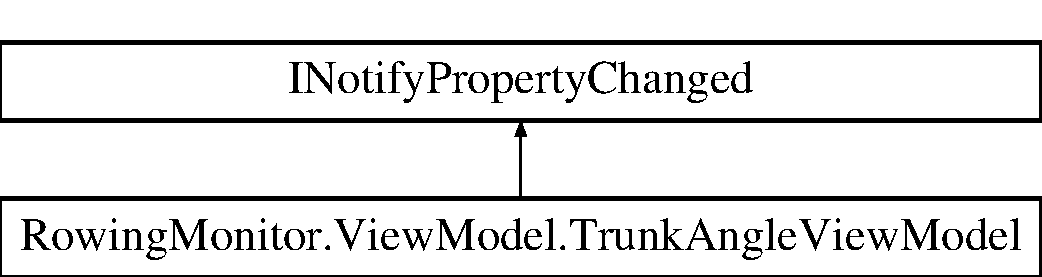
\includegraphics[height=2.000000cm]{class_rowing_monitor_1_1_view_model_1_1_trunk_angle_view_model}
\end{center}
\end{figure}
\subsection*{Public Member Functions}
\begin{DoxyCompactItemize}
\item 
\hyperlink{class_rowing_monitor_1_1_view_model_1_1_trunk_angle_view_model_a66b6cf452c62d64c865b7fdda61edbcb}{Trunk\+Angle\+View\+Model} ()
\item 
void \hyperlink{class_rowing_monitor_1_1_view_model_1_1_trunk_angle_view_model_ad6a2b70f86e46a2c60b90a77fa57e645}{Render} (double catch\+Trunk\+Angle, double finish\+Trunk\+Angle, double trunk\+Angle)
\end{DoxyCompactItemize}
\subsection*{Properties}
\begin{DoxyCompactItemize}
\item 
double \hyperlink{class_rowing_monitor_1_1_view_model_1_1_trunk_angle_view_model_a64fc2e1372e05c65cd17f24a142f2783}{Catch\+Trunk\+Angle}\hspace{0.3cm}{\ttfamily  \mbox{[}get, set\mbox{]}}
\item 
double \hyperlink{class_rowing_monitor_1_1_view_model_1_1_trunk_angle_view_model_a2eeeab2ed9f562381aff8e7d8f8e19c6}{Finish\+Trunk\+Angle}\hspace{0.3cm}{\ttfamily  \mbox{[}get, set\mbox{]}}
\item 
double \hyperlink{class_rowing_monitor_1_1_view_model_1_1_trunk_angle_view_model_af5df9632377df43618457ce9743e2793}{Trunk\+Angle}\hspace{0.3cm}{\ttfamily  \mbox{[}get, set\mbox{]}}
\item 
string \hyperlink{class_rowing_monitor_1_1_view_model_1_1_trunk_angle_view_model_a696475d48415b0f2d9574d9189eac534}{Catch\+Trunk\+Angle\+String}\hspace{0.3cm}{\ttfamily  \mbox{[}get, set\mbox{]}}
\item 
string \hyperlink{class_rowing_monitor_1_1_view_model_1_1_trunk_angle_view_model_a655f421edb6375f54ae79af3207014cd}{Finish\+Trunk\+Angle\+String}\hspace{0.3cm}{\ttfamily  \mbox{[}get, set\mbox{]}}
\item 
string \hyperlink{class_rowing_monitor_1_1_view_model_1_1_trunk_angle_view_model_adfd95524f3e943d219f72ffee09a9040}{Trunk\+Angle\+String}\hspace{0.3cm}{\ttfamily  \mbox{[}get, set\mbox{]}}
\end{DoxyCompactItemize}
\subsection*{Events}
\begin{DoxyCompactItemize}
\item 
Property\+Changed\+Event\+Handler \hyperlink{class_rowing_monitor_1_1_view_model_1_1_trunk_angle_view_model_afbf525541d69036a9e40d427d08084c1}{Property\+Changed}
\end{DoxyCompactItemize}


\subsection{Constructor \& Destructor Documentation}
\mbox{\Hypertarget{class_rowing_monitor_1_1_view_model_1_1_trunk_angle_view_model_a66b6cf452c62d64c865b7fdda61edbcb}\label{class_rowing_monitor_1_1_view_model_1_1_trunk_angle_view_model_a66b6cf452c62d64c865b7fdda61edbcb}} 
\index{Rowing\+Monitor\+::\+View\+Model\+::\+Trunk\+Angle\+View\+Model@{Rowing\+Monitor\+::\+View\+Model\+::\+Trunk\+Angle\+View\+Model}!Trunk\+Angle\+View\+Model@{Trunk\+Angle\+View\+Model}}
\index{Trunk\+Angle\+View\+Model@{Trunk\+Angle\+View\+Model}!Rowing\+Monitor\+::\+View\+Model\+::\+Trunk\+Angle\+View\+Model@{Rowing\+Monitor\+::\+View\+Model\+::\+Trunk\+Angle\+View\+Model}}
\subsubsection{\texorpdfstring{Trunk\+Angle\+View\+Model()}{TrunkAngleViewModel()}}
{\footnotesize\ttfamily Rowing\+Monitor.\+View\+Model.\+Trunk\+Angle\+View\+Model.\+Trunk\+Angle\+View\+Model (\begin{DoxyParamCaption}{ }\end{DoxyParamCaption})}



\subsection{Member Function Documentation}
\mbox{\Hypertarget{class_rowing_monitor_1_1_view_model_1_1_trunk_angle_view_model_ad6a2b70f86e46a2c60b90a77fa57e645}\label{class_rowing_monitor_1_1_view_model_1_1_trunk_angle_view_model_ad6a2b70f86e46a2c60b90a77fa57e645}} 
\index{Rowing\+Monitor\+::\+View\+Model\+::\+Trunk\+Angle\+View\+Model@{Rowing\+Monitor\+::\+View\+Model\+::\+Trunk\+Angle\+View\+Model}!Render@{Render}}
\index{Render@{Render}!Rowing\+Monitor\+::\+View\+Model\+::\+Trunk\+Angle\+View\+Model@{Rowing\+Monitor\+::\+View\+Model\+::\+Trunk\+Angle\+View\+Model}}
\subsubsection{\texorpdfstring{Render()}{Render()}}
{\footnotesize\ttfamily void Rowing\+Monitor.\+View\+Model.\+Trunk\+Angle\+View\+Model.\+Render (\begin{DoxyParamCaption}\item[{double}]{catch\+Trunk\+Angle,  }\item[{double}]{finish\+Trunk\+Angle,  }\item[{double}]{trunk\+Angle }\end{DoxyParamCaption})}



\subsection{Property Documentation}
\mbox{\Hypertarget{class_rowing_monitor_1_1_view_model_1_1_trunk_angle_view_model_a64fc2e1372e05c65cd17f24a142f2783}\label{class_rowing_monitor_1_1_view_model_1_1_trunk_angle_view_model_a64fc2e1372e05c65cd17f24a142f2783}} 
\index{Rowing\+Monitor\+::\+View\+Model\+::\+Trunk\+Angle\+View\+Model@{Rowing\+Monitor\+::\+View\+Model\+::\+Trunk\+Angle\+View\+Model}!Catch\+Trunk\+Angle@{Catch\+Trunk\+Angle}}
\index{Catch\+Trunk\+Angle@{Catch\+Trunk\+Angle}!Rowing\+Monitor\+::\+View\+Model\+::\+Trunk\+Angle\+View\+Model@{Rowing\+Monitor\+::\+View\+Model\+::\+Trunk\+Angle\+View\+Model}}
\subsubsection{\texorpdfstring{Catch\+Trunk\+Angle}{CatchTrunkAngle}}
{\footnotesize\ttfamily double Rowing\+Monitor.\+View\+Model.\+Trunk\+Angle\+View\+Model.\+Catch\+Trunk\+Angle\hspace{0.3cm}{\ttfamily [get]}, {\ttfamily [set]}}

\mbox{\Hypertarget{class_rowing_monitor_1_1_view_model_1_1_trunk_angle_view_model_a696475d48415b0f2d9574d9189eac534}\label{class_rowing_monitor_1_1_view_model_1_1_trunk_angle_view_model_a696475d48415b0f2d9574d9189eac534}} 
\index{Rowing\+Monitor\+::\+View\+Model\+::\+Trunk\+Angle\+View\+Model@{Rowing\+Monitor\+::\+View\+Model\+::\+Trunk\+Angle\+View\+Model}!Catch\+Trunk\+Angle\+String@{Catch\+Trunk\+Angle\+String}}
\index{Catch\+Trunk\+Angle\+String@{Catch\+Trunk\+Angle\+String}!Rowing\+Monitor\+::\+View\+Model\+::\+Trunk\+Angle\+View\+Model@{Rowing\+Monitor\+::\+View\+Model\+::\+Trunk\+Angle\+View\+Model}}
\subsubsection{\texorpdfstring{Catch\+Trunk\+Angle\+String}{CatchTrunkAngleString}}
{\footnotesize\ttfamily string Rowing\+Monitor.\+View\+Model.\+Trunk\+Angle\+View\+Model.\+Catch\+Trunk\+Angle\+String\hspace{0.3cm}{\ttfamily [get]}, {\ttfamily [set]}}

\mbox{\Hypertarget{class_rowing_monitor_1_1_view_model_1_1_trunk_angle_view_model_a2eeeab2ed9f562381aff8e7d8f8e19c6}\label{class_rowing_monitor_1_1_view_model_1_1_trunk_angle_view_model_a2eeeab2ed9f562381aff8e7d8f8e19c6}} 
\index{Rowing\+Monitor\+::\+View\+Model\+::\+Trunk\+Angle\+View\+Model@{Rowing\+Monitor\+::\+View\+Model\+::\+Trunk\+Angle\+View\+Model}!Finish\+Trunk\+Angle@{Finish\+Trunk\+Angle}}
\index{Finish\+Trunk\+Angle@{Finish\+Trunk\+Angle}!Rowing\+Monitor\+::\+View\+Model\+::\+Trunk\+Angle\+View\+Model@{Rowing\+Monitor\+::\+View\+Model\+::\+Trunk\+Angle\+View\+Model}}
\subsubsection{\texorpdfstring{Finish\+Trunk\+Angle}{FinishTrunkAngle}}
{\footnotesize\ttfamily double Rowing\+Monitor.\+View\+Model.\+Trunk\+Angle\+View\+Model.\+Finish\+Trunk\+Angle\hspace{0.3cm}{\ttfamily [get]}, {\ttfamily [set]}}

\mbox{\Hypertarget{class_rowing_monitor_1_1_view_model_1_1_trunk_angle_view_model_a655f421edb6375f54ae79af3207014cd}\label{class_rowing_monitor_1_1_view_model_1_1_trunk_angle_view_model_a655f421edb6375f54ae79af3207014cd}} 
\index{Rowing\+Monitor\+::\+View\+Model\+::\+Trunk\+Angle\+View\+Model@{Rowing\+Monitor\+::\+View\+Model\+::\+Trunk\+Angle\+View\+Model}!Finish\+Trunk\+Angle\+String@{Finish\+Trunk\+Angle\+String}}
\index{Finish\+Trunk\+Angle\+String@{Finish\+Trunk\+Angle\+String}!Rowing\+Monitor\+::\+View\+Model\+::\+Trunk\+Angle\+View\+Model@{Rowing\+Monitor\+::\+View\+Model\+::\+Trunk\+Angle\+View\+Model}}
\subsubsection{\texorpdfstring{Finish\+Trunk\+Angle\+String}{FinishTrunkAngleString}}
{\footnotesize\ttfamily string Rowing\+Monitor.\+View\+Model.\+Trunk\+Angle\+View\+Model.\+Finish\+Trunk\+Angle\+String\hspace{0.3cm}{\ttfamily [get]}, {\ttfamily [set]}}

\mbox{\Hypertarget{class_rowing_monitor_1_1_view_model_1_1_trunk_angle_view_model_af5df9632377df43618457ce9743e2793}\label{class_rowing_monitor_1_1_view_model_1_1_trunk_angle_view_model_af5df9632377df43618457ce9743e2793}} 
\index{Rowing\+Monitor\+::\+View\+Model\+::\+Trunk\+Angle\+View\+Model@{Rowing\+Monitor\+::\+View\+Model\+::\+Trunk\+Angle\+View\+Model}!Trunk\+Angle@{Trunk\+Angle}}
\index{Trunk\+Angle@{Trunk\+Angle}!Rowing\+Monitor\+::\+View\+Model\+::\+Trunk\+Angle\+View\+Model@{Rowing\+Monitor\+::\+View\+Model\+::\+Trunk\+Angle\+View\+Model}}
\subsubsection{\texorpdfstring{Trunk\+Angle}{TrunkAngle}}
{\footnotesize\ttfamily double Rowing\+Monitor.\+View\+Model.\+Trunk\+Angle\+View\+Model.\+Trunk\+Angle\hspace{0.3cm}{\ttfamily [get]}, {\ttfamily [set]}}

\mbox{\Hypertarget{class_rowing_monitor_1_1_view_model_1_1_trunk_angle_view_model_adfd95524f3e943d219f72ffee09a9040}\label{class_rowing_monitor_1_1_view_model_1_1_trunk_angle_view_model_adfd95524f3e943d219f72ffee09a9040}} 
\index{Rowing\+Monitor\+::\+View\+Model\+::\+Trunk\+Angle\+View\+Model@{Rowing\+Monitor\+::\+View\+Model\+::\+Trunk\+Angle\+View\+Model}!Trunk\+Angle\+String@{Trunk\+Angle\+String}}
\index{Trunk\+Angle\+String@{Trunk\+Angle\+String}!Rowing\+Monitor\+::\+View\+Model\+::\+Trunk\+Angle\+View\+Model@{Rowing\+Monitor\+::\+View\+Model\+::\+Trunk\+Angle\+View\+Model}}
\subsubsection{\texorpdfstring{Trunk\+Angle\+String}{TrunkAngleString}}
{\footnotesize\ttfamily string Rowing\+Monitor.\+View\+Model.\+Trunk\+Angle\+View\+Model.\+Trunk\+Angle\+String\hspace{0.3cm}{\ttfamily [get]}, {\ttfamily [set]}}



\subsection{Event Documentation}
\mbox{\Hypertarget{class_rowing_monitor_1_1_view_model_1_1_trunk_angle_view_model_afbf525541d69036a9e40d427d08084c1}\label{class_rowing_monitor_1_1_view_model_1_1_trunk_angle_view_model_afbf525541d69036a9e40d427d08084c1}} 
\index{Rowing\+Monitor\+::\+View\+Model\+::\+Trunk\+Angle\+View\+Model@{Rowing\+Monitor\+::\+View\+Model\+::\+Trunk\+Angle\+View\+Model}!Property\+Changed@{Property\+Changed}}
\index{Property\+Changed@{Property\+Changed}!Rowing\+Monitor\+::\+View\+Model\+::\+Trunk\+Angle\+View\+Model@{Rowing\+Monitor\+::\+View\+Model\+::\+Trunk\+Angle\+View\+Model}}
\subsubsection{\texorpdfstring{Property\+Changed}{PropertyChanged}}
{\footnotesize\ttfamily Property\+Changed\+Event\+Handler Rowing\+Monitor.\+View\+Model.\+Trunk\+Angle\+View\+Model.\+Property\+Changed}



The documentation for this class was generated from the following file\+:\begin{DoxyCompactItemize}
\item 
View\+Model/\hyperlink{_trunk_angle_view_model_8cs}{Trunk\+Angle\+View\+Model.\+cs}\end{DoxyCompactItemize}

\hypertarget{class_rowing_monitor_1_1_model_1_1_pipeline_1_1_velocity_calculator}{}\section{Rowing\+Monitor.\+Model.\+Pipeline.\+Velocity\+Calculator Class Reference}
\label{class_rowing_monitor_1_1_model_1_1_pipeline_1_1_velocity_calculator}\index{Rowing\+Monitor.\+Model.\+Pipeline.\+Velocity\+Calculator@{Rowing\+Monitor.\+Model.\+Pipeline.\+Velocity\+Calculator}}
\subsection*{Public Member Functions}
\begin{DoxyCompactItemize}
\item 
delegate void \hyperlink{class_rowing_monitor_1_1_model_1_1_pipeline_1_1_velocity_calculator_a8788be37e2e5ff495980455003f16b94}{Calculated\+Frame\+Arrived\+Event\+Handler} (Object sender, \hyperlink{class_rowing_monitor_1_1_model_1_1_calculated_frame_arrived_event_args}{Calculated\+Frame\+Arrived\+Event\+Args} e)
\item 
\hyperlink{class_rowing_monitor_1_1_model_1_1_pipeline_1_1_velocity_calculator_acb35632a51a3bdcb33410a46ed7ac210}{Velocity\+Calculator} ()
\item 
void \hyperlink{class_rowing_monitor_1_1_model_1_1_pipeline_1_1_velocity_calculator_a6e39f143e7cbb1c99eb6f74734dc3be3}{Update} (\hyperlink{struct_rowing_monitor_1_1_model_1_1_util_1_1_joint_data}{Joint\+Data} joint\+Data)
\item 
\hyperlink{struct_rowing_monitor_1_1_model_1_1_util_1_1_joint_data}{Joint\+Data} \hyperlink{class_rowing_monitor_1_1_model_1_1_pipeline_1_1_velocity_calculator_a679bdfdc1c2c8886cbf5dd329c7f5ee6}{Calculate\+Velocity} (\hyperlink{struct_rowing_monitor_1_1_model_1_1_util_1_1_joint_data}{Joint\+Data} joint\+Data)
\begin{DoxyCompactList}\small\item\em Calculates the velocity as 1st derivative (gradient) of position. Calculation needs one frame as buffer. \end{DoxyCompactList}\end{DoxyCompactItemize}
\subsection*{Properties}
\begin{DoxyCompactItemize}
\item 
Broadcast\+Block$<$ \hyperlink{struct_rowing_monitor_1_1_model_1_1_util_1_1_joint_data}{Joint\+Data} $>$ \hyperlink{class_rowing_monitor_1_1_model_1_1_pipeline_1_1_velocity_calculator_ac10c38181683a7ec3493d5bb590b9d06}{Output}\hspace{0.3cm}{\ttfamily  \mbox{[}get, set\mbox{]}}
\item 
Action\+Block$<$ \hyperlink{struct_rowing_monitor_1_1_model_1_1_util_1_1_joint_data}{Joint\+Data} $>$ \hyperlink{class_rowing_monitor_1_1_model_1_1_pipeline_1_1_velocity_calculator_a4088ab5421155308f4c0a2cc5eb2a3da}{Input}\hspace{0.3cm}{\ttfamily  \mbox{[}get, set\mbox{]}}
\end{DoxyCompactItemize}
\subsection*{Events}
\begin{DoxyCompactItemize}
\item 
\hyperlink{class_rowing_monitor_1_1_model_1_1_pipeline_1_1_velocity_calculator_a8788be37e2e5ff495980455003f16b94}{Calculated\+Frame\+Arrived\+Event\+Handler} \hyperlink{class_rowing_monitor_1_1_model_1_1_pipeline_1_1_velocity_calculator_ad0b95bfb006ea268ea476f1da13bc7da}{Calculated\+Frame\+Arrived}
\end{DoxyCompactItemize}


\subsection{Constructor \& Destructor Documentation}
\mbox{\Hypertarget{class_rowing_monitor_1_1_model_1_1_pipeline_1_1_velocity_calculator_acb35632a51a3bdcb33410a46ed7ac210}\label{class_rowing_monitor_1_1_model_1_1_pipeline_1_1_velocity_calculator_acb35632a51a3bdcb33410a46ed7ac210}} 
\index{Rowing\+Monitor\+::\+Model\+::\+Pipeline\+::\+Velocity\+Calculator@{Rowing\+Monitor\+::\+Model\+::\+Pipeline\+::\+Velocity\+Calculator}!Velocity\+Calculator@{Velocity\+Calculator}}
\index{Velocity\+Calculator@{Velocity\+Calculator}!Rowing\+Monitor\+::\+Model\+::\+Pipeline\+::\+Velocity\+Calculator@{Rowing\+Monitor\+::\+Model\+::\+Pipeline\+::\+Velocity\+Calculator}}
\subsubsection{\texorpdfstring{Velocity\+Calculator()}{VelocityCalculator()}}
{\footnotesize\ttfamily Rowing\+Monitor.\+Model.\+Pipeline.\+Velocity\+Calculator.\+Velocity\+Calculator (\begin{DoxyParamCaption}{ }\end{DoxyParamCaption})}



\subsection{Member Function Documentation}
\mbox{\Hypertarget{class_rowing_monitor_1_1_model_1_1_pipeline_1_1_velocity_calculator_a8788be37e2e5ff495980455003f16b94}\label{class_rowing_monitor_1_1_model_1_1_pipeline_1_1_velocity_calculator_a8788be37e2e5ff495980455003f16b94}} 
\index{Rowing\+Monitor\+::\+Model\+::\+Pipeline\+::\+Velocity\+Calculator@{Rowing\+Monitor\+::\+Model\+::\+Pipeline\+::\+Velocity\+Calculator}!Calculated\+Frame\+Arrived\+Event\+Handler@{Calculated\+Frame\+Arrived\+Event\+Handler}}
\index{Calculated\+Frame\+Arrived\+Event\+Handler@{Calculated\+Frame\+Arrived\+Event\+Handler}!Rowing\+Monitor\+::\+Model\+::\+Pipeline\+::\+Velocity\+Calculator@{Rowing\+Monitor\+::\+Model\+::\+Pipeline\+::\+Velocity\+Calculator}}
\subsubsection{\texorpdfstring{Calculated\+Frame\+Arrived\+Event\+Handler()}{CalculatedFrameArrivedEventHandler()}}
{\footnotesize\ttfamily delegate void Rowing\+Monitor.\+Model.\+Pipeline.\+Velocity\+Calculator.\+Calculated\+Frame\+Arrived\+Event\+Handler (\begin{DoxyParamCaption}\item[{Object}]{sender,  }\item[{\hyperlink{class_rowing_monitor_1_1_model_1_1_calculated_frame_arrived_event_args}{Calculated\+Frame\+Arrived\+Event\+Args}}]{e }\end{DoxyParamCaption})}

\mbox{\Hypertarget{class_rowing_monitor_1_1_model_1_1_pipeline_1_1_velocity_calculator_a679bdfdc1c2c8886cbf5dd329c7f5ee6}\label{class_rowing_monitor_1_1_model_1_1_pipeline_1_1_velocity_calculator_a679bdfdc1c2c8886cbf5dd329c7f5ee6}} 
\index{Rowing\+Monitor\+::\+Model\+::\+Pipeline\+::\+Velocity\+Calculator@{Rowing\+Monitor\+::\+Model\+::\+Pipeline\+::\+Velocity\+Calculator}!Calculate\+Velocity@{Calculate\+Velocity}}
\index{Calculate\+Velocity@{Calculate\+Velocity}!Rowing\+Monitor\+::\+Model\+::\+Pipeline\+::\+Velocity\+Calculator@{Rowing\+Monitor\+::\+Model\+::\+Pipeline\+::\+Velocity\+Calculator}}
\subsubsection{\texorpdfstring{Calculate\+Velocity()}{CalculateVelocity()}}
{\footnotesize\ttfamily \hyperlink{struct_rowing_monitor_1_1_model_1_1_util_1_1_joint_data}{Joint\+Data} Rowing\+Monitor.\+Model.\+Pipeline.\+Velocity\+Calculator.\+Calculate\+Velocity (\begin{DoxyParamCaption}\item[{\hyperlink{struct_rowing_monitor_1_1_model_1_1_util_1_1_joint_data}{Joint\+Data}}]{joint\+Data }\end{DoxyParamCaption})}



Calculates the velocity as 1st derivative (gradient) of position. Calculation needs one frame as buffer. 


\begin{DoxyParams}{Parameters}
{\em joint\+Data} & \\
\hline
\end{DoxyParams}
\mbox{\Hypertarget{class_rowing_monitor_1_1_model_1_1_pipeline_1_1_velocity_calculator_a6e39f143e7cbb1c99eb6f74734dc3be3}\label{class_rowing_monitor_1_1_model_1_1_pipeline_1_1_velocity_calculator_a6e39f143e7cbb1c99eb6f74734dc3be3}} 
\index{Rowing\+Monitor\+::\+Model\+::\+Pipeline\+::\+Velocity\+Calculator@{Rowing\+Monitor\+::\+Model\+::\+Pipeline\+::\+Velocity\+Calculator}!Update@{Update}}
\index{Update@{Update}!Rowing\+Monitor\+::\+Model\+::\+Pipeline\+::\+Velocity\+Calculator@{Rowing\+Monitor\+::\+Model\+::\+Pipeline\+::\+Velocity\+Calculator}}
\subsubsection{\texorpdfstring{Update()}{Update()}}
{\footnotesize\ttfamily void Rowing\+Monitor.\+Model.\+Pipeline.\+Velocity\+Calculator.\+Update (\begin{DoxyParamCaption}\item[{\hyperlink{struct_rowing_monitor_1_1_model_1_1_util_1_1_joint_data}{Joint\+Data}}]{joint\+Data }\end{DoxyParamCaption})}



\subsection{Property Documentation}
\mbox{\Hypertarget{class_rowing_monitor_1_1_model_1_1_pipeline_1_1_velocity_calculator_a4088ab5421155308f4c0a2cc5eb2a3da}\label{class_rowing_monitor_1_1_model_1_1_pipeline_1_1_velocity_calculator_a4088ab5421155308f4c0a2cc5eb2a3da}} 
\index{Rowing\+Monitor\+::\+Model\+::\+Pipeline\+::\+Velocity\+Calculator@{Rowing\+Monitor\+::\+Model\+::\+Pipeline\+::\+Velocity\+Calculator}!Input@{Input}}
\index{Input@{Input}!Rowing\+Monitor\+::\+Model\+::\+Pipeline\+::\+Velocity\+Calculator@{Rowing\+Monitor\+::\+Model\+::\+Pipeline\+::\+Velocity\+Calculator}}
\subsubsection{\texorpdfstring{Input}{Input}}
{\footnotesize\ttfamily Action\+Block$<$\hyperlink{struct_rowing_monitor_1_1_model_1_1_util_1_1_joint_data}{Joint\+Data}$>$ Rowing\+Monitor.\+Model.\+Pipeline.\+Velocity\+Calculator.\+Input\hspace{0.3cm}{\ttfamily [get]}, {\ttfamily [set]}}

\mbox{\Hypertarget{class_rowing_monitor_1_1_model_1_1_pipeline_1_1_velocity_calculator_ac10c38181683a7ec3493d5bb590b9d06}\label{class_rowing_monitor_1_1_model_1_1_pipeline_1_1_velocity_calculator_ac10c38181683a7ec3493d5bb590b9d06}} 
\index{Rowing\+Monitor\+::\+Model\+::\+Pipeline\+::\+Velocity\+Calculator@{Rowing\+Monitor\+::\+Model\+::\+Pipeline\+::\+Velocity\+Calculator}!Output@{Output}}
\index{Output@{Output}!Rowing\+Monitor\+::\+Model\+::\+Pipeline\+::\+Velocity\+Calculator@{Rowing\+Monitor\+::\+Model\+::\+Pipeline\+::\+Velocity\+Calculator}}
\subsubsection{\texorpdfstring{Output}{Output}}
{\footnotesize\ttfamily Broadcast\+Block$<$\hyperlink{struct_rowing_monitor_1_1_model_1_1_util_1_1_joint_data}{Joint\+Data}$>$ Rowing\+Monitor.\+Model.\+Pipeline.\+Velocity\+Calculator.\+Output\hspace{0.3cm}{\ttfamily [get]}, {\ttfamily [set]}}



\subsection{Event Documentation}
\mbox{\Hypertarget{class_rowing_monitor_1_1_model_1_1_pipeline_1_1_velocity_calculator_ad0b95bfb006ea268ea476f1da13bc7da}\label{class_rowing_monitor_1_1_model_1_1_pipeline_1_1_velocity_calculator_ad0b95bfb006ea268ea476f1da13bc7da}} 
\index{Rowing\+Monitor\+::\+Model\+::\+Pipeline\+::\+Velocity\+Calculator@{Rowing\+Monitor\+::\+Model\+::\+Pipeline\+::\+Velocity\+Calculator}!Calculated\+Frame\+Arrived@{Calculated\+Frame\+Arrived}}
\index{Calculated\+Frame\+Arrived@{Calculated\+Frame\+Arrived}!Rowing\+Monitor\+::\+Model\+::\+Pipeline\+::\+Velocity\+Calculator@{Rowing\+Monitor\+::\+Model\+::\+Pipeline\+::\+Velocity\+Calculator}}
\subsubsection{\texorpdfstring{Calculated\+Frame\+Arrived}{CalculatedFrameArrived}}
{\footnotesize\ttfamily \hyperlink{class_rowing_monitor_1_1_model_1_1_pipeline_1_1_velocity_calculator_a8788be37e2e5ff495980455003f16b94}{Calculated\+Frame\+Arrived\+Event\+Handler} Rowing\+Monitor.\+Model.\+Pipeline.\+Velocity\+Calculator.\+Calculated\+Frame\+Arrived}



The documentation for this class was generated from the following file\+:\begin{DoxyCompactItemize}
\item 
Model/\+Pipeline/\hyperlink{_velocity_calculator_8cs}{Velocity\+Calculator.\+cs}\end{DoxyCompactItemize}

\hypertarget{class_rowing_monitor_1_1_model_1_1_pipeline_1_1_z_v_c_segment_detector}{}\section{Rowing\+Monitor.\+Model.\+Pipeline.\+Z\+V\+C\+Segment\+Detector Class Reference}
\label{class_rowing_monitor_1_1_model_1_1_pipeline_1_1_z_v_c_segment_detector}\index{Rowing\+Monitor.\+Model.\+Pipeline.\+Z\+V\+C\+Segment\+Detector@{Rowing\+Monitor.\+Model.\+Pipeline.\+Z\+V\+C\+Segment\+Detector}}
Inheritance diagram for Rowing\+Monitor.\+Model.\+Pipeline.\+Z\+V\+C\+Segment\+Detector\+:\begin{figure}[H]
\begin{center}
\leavevmode
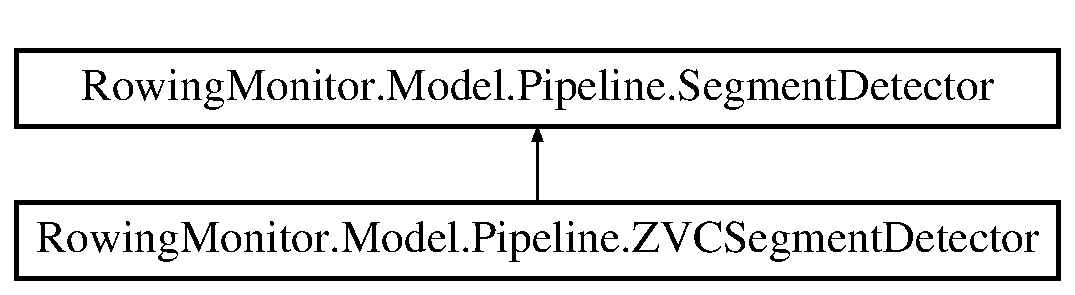
\includegraphics[height=2.000000cm]{class_rowing_monitor_1_1_model_1_1_pipeline_1_1_z_v_c_segment_detector}
\end{center}
\end{figure}
\subsection*{Public Member Functions}
\begin{DoxyCompactItemize}
\item 
\hyperlink{class_rowing_monitor_1_1_model_1_1_pipeline_1_1_z_v_c_segment_detector_ae8612877f3f7310db743529f61547616}{Z\+V\+C\+Segment\+Detector} (int minimum\+Hit\+Gap, bool start\+Segment\+With\+Rising\+Velocity=true)
\begin{DoxyCompactList}\small\item\em Creates a new zero velocity segment detector. \end{DoxyCompactList}\item 
override void \hyperlink{class_rowing_monitor_1_1_model_1_1_pipeline_1_1_z_v_c_segment_detector_a81c28e4ede1561c2fe1eca29f63f0767}{Update} (\hyperlink{struct_rowing_monitor_1_1_model_1_1_util_1_1_joint_data}{Joint\+Data} joint\+Data, Joint\+Type joint\+Type, String axis)
\item 
override List$<$ \hyperlink{struct_rowing_monitor_1_1_model_1_1_util_1_1_segment_hit}{Segment\+Hit} $>$ \hyperlink{class_rowing_monitor_1_1_model_1_1_pipeline_1_1_z_v_c_segment_detector_afc9e7a0ab77b102a7fcd1bb3d216763d}{Detect} (\hyperlink{struct_rowing_monitor_1_1_model_1_1_util_1_1_joint_data}{Joint\+Data} joint\+Data, Joint\+Type joint\+Type, string axis)
\end{DoxyCompactItemize}
\subsection*{Protected Member Functions}
\begin{DoxyCompactItemize}
\item 
override void \hyperlink{class_rowing_monitor_1_1_model_1_1_pipeline_1_1_z_v_c_segment_detector_a5eab838eda9f217722dfa05bc9d5095b}{On\+Segment\+Detected} (\hyperlink{class_rowing_monitor_1_1_model_1_1_segment_detected_event_args}{Segment\+Detected\+Event\+Args} e)
\end{DoxyCompactItemize}
\subsection*{Additional Inherited Members}


\subsection{Constructor \& Destructor Documentation}
\mbox{\Hypertarget{class_rowing_monitor_1_1_model_1_1_pipeline_1_1_z_v_c_segment_detector_ae8612877f3f7310db743529f61547616}\label{class_rowing_monitor_1_1_model_1_1_pipeline_1_1_z_v_c_segment_detector_ae8612877f3f7310db743529f61547616}} 
\index{Rowing\+Monitor\+::\+Model\+::\+Pipeline\+::\+Z\+V\+C\+Segment\+Detector@{Rowing\+Monitor\+::\+Model\+::\+Pipeline\+::\+Z\+V\+C\+Segment\+Detector}!Z\+V\+C\+Segment\+Detector@{Z\+V\+C\+Segment\+Detector}}
\index{Z\+V\+C\+Segment\+Detector@{Z\+V\+C\+Segment\+Detector}!Rowing\+Monitor\+::\+Model\+::\+Pipeline\+::\+Z\+V\+C\+Segment\+Detector@{Rowing\+Monitor\+::\+Model\+::\+Pipeline\+::\+Z\+V\+C\+Segment\+Detector}}
\subsubsection{\texorpdfstring{Z\+V\+C\+Segment\+Detector()}{ZVCSegmentDetector()}}
{\footnotesize\ttfamily Rowing\+Monitor.\+Model.\+Pipeline.\+Z\+V\+C\+Segment\+Detector.\+Z\+V\+C\+Segment\+Detector (\begin{DoxyParamCaption}\item[{int}]{minimum\+Hit\+Gap,  }\item[{bool}]{start\+Segment\+With\+Rising\+Velocity = {\ttfamily true} }\end{DoxyParamCaption})}



Creates a new zero velocity segment detector. 


\begin{DoxyParams}{Parameters}
{\em minimum\+Hit\+Gap} & Minimum count ouf indices between two hits.\\
\hline
{\em start\+Segment\+With\+Rising\+Velocity} & Define if the start/end point of a segment has a rising or falling slope\\
\hline
\end{DoxyParams}


\subsection{Member Function Documentation}
\mbox{\Hypertarget{class_rowing_monitor_1_1_model_1_1_pipeline_1_1_z_v_c_segment_detector_afc9e7a0ab77b102a7fcd1bb3d216763d}\label{class_rowing_monitor_1_1_model_1_1_pipeline_1_1_z_v_c_segment_detector_afc9e7a0ab77b102a7fcd1bb3d216763d}} 
\index{Rowing\+Monitor\+::\+Model\+::\+Pipeline\+::\+Z\+V\+C\+Segment\+Detector@{Rowing\+Monitor\+::\+Model\+::\+Pipeline\+::\+Z\+V\+C\+Segment\+Detector}!Detect@{Detect}}
\index{Detect@{Detect}!Rowing\+Monitor\+::\+Model\+::\+Pipeline\+::\+Z\+V\+C\+Segment\+Detector@{Rowing\+Monitor\+::\+Model\+::\+Pipeline\+::\+Z\+V\+C\+Segment\+Detector}}
\subsubsection{\texorpdfstring{Detect()}{Detect()}}
{\footnotesize\ttfamily override List$<$\hyperlink{struct_rowing_monitor_1_1_model_1_1_util_1_1_segment_hit}{Segment\+Hit}$>$ Rowing\+Monitor.\+Model.\+Pipeline.\+Z\+V\+C\+Segment\+Detector.\+Detect (\begin{DoxyParamCaption}\item[{\hyperlink{struct_rowing_monitor_1_1_model_1_1_util_1_1_joint_data}{Joint\+Data}}]{joint\+Data,  }\item[{Joint\+Type}]{joint\+Type,  }\item[{string}]{axis }\end{DoxyParamCaption})}

\mbox{\Hypertarget{class_rowing_monitor_1_1_model_1_1_pipeline_1_1_z_v_c_segment_detector_a5eab838eda9f217722dfa05bc9d5095b}\label{class_rowing_monitor_1_1_model_1_1_pipeline_1_1_z_v_c_segment_detector_a5eab838eda9f217722dfa05bc9d5095b}} 
\index{Rowing\+Monitor\+::\+Model\+::\+Pipeline\+::\+Z\+V\+C\+Segment\+Detector@{Rowing\+Monitor\+::\+Model\+::\+Pipeline\+::\+Z\+V\+C\+Segment\+Detector}!On\+Segment\+Detected@{On\+Segment\+Detected}}
\index{On\+Segment\+Detected@{On\+Segment\+Detected}!Rowing\+Monitor\+::\+Model\+::\+Pipeline\+::\+Z\+V\+C\+Segment\+Detector@{Rowing\+Monitor\+::\+Model\+::\+Pipeline\+::\+Z\+V\+C\+Segment\+Detector}}
\subsubsection{\texorpdfstring{On\+Segment\+Detected()}{OnSegmentDetected()}}
{\footnotesize\ttfamily override void Rowing\+Monitor.\+Model.\+Pipeline.\+Z\+V\+C\+Segment\+Detector.\+On\+Segment\+Detected (\begin{DoxyParamCaption}\item[{\hyperlink{class_rowing_monitor_1_1_model_1_1_segment_detected_event_args}{Segment\+Detected\+Event\+Args}}]{e }\end{DoxyParamCaption})\hspace{0.3cm}{\ttfamily [protected]}, {\ttfamily [virtual]}}



Reimplemented from \hyperlink{class_rowing_monitor_1_1_model_1_1_pipeline_1_1_segment_detector_a30d5b8752257a3992db11770506f6a8a}{Rowing\+Monitor.\+Model.\+Pipeline.\+Segment\+Detector}.

\mbox{\Hypertarget{class_rowing_monitor_1_1_model_1_1_pipeline_1_1_z_v_c_segment_detector_a81c28e4ede1561c2fe1eca29f63f0767}\label{class_rowing_monitor_1_1_model_1_1_pipeline_1_1_z_v_c_segment_detector_a81c28e4ede1561c2fe1eca29f63f0767}} 
\index{Rowing\+Monitor\+::\+Model\+::\+Pipeline\+::\+Z\+V\+C\+Segment\+Detector@{Rowing\+Monitor\+::\+Model\+::\+Pipeline\+::\+Z\+V\+C\+Segment\+Detector}!Update@{Update}}
\index{Update@{Update}!Rowing\+Monitor\+::\+Model\+::\+Pipeline\+::\+Z\+V\+C\+Segment\+Detector@{Rowing\+Monitor\+::\+Model\+::\+Pipeline\+::\+Z\+V\+C\+Segment\+Detector}}
\subsubsection{\texorpdfstring{Update()}{Update()}}
{\footnotesize\ttfamily override void Rowing\+Monitor.\+Model.\+Pipeline.\+Z\+V\+C\+Segment\+Detector.\+Update (\begin{DoxyParamCaption}\item[{\hyperlink{struct_rowing_monitor_1_1_model_1_1_util_1_1_joint_data}{Joint\+Data}}]{joint\+Data,  }\item[{Joint\+Type}]{joint\+Type,  }\item[{String}]{axis }\end{DoxyParamCaption})\hspace{0.3cm}{\ttfamily [virtual]}}



Implements \hyperlink{class_rowing_monitor_1_1_model_1_1_pipeline_1_1_segment_detector_a24dcb2926660a6218af3052f147d82da}{Rowing\+Monitor.\+Model.\+Pipeline.\+Segment\+Detector}.



The documentation for this class was generated from the following file\+:\begin{DoxyCompactItemize}
\item 
Model/\+Pipeline/\hyperlink{_z_v_c_segment_detector_8cs}{Z\+V\+C\+Segment\+Detector.\+cs}\end{DoxyCompactItemize}

\chapter{File Documentation}
\hypertarget{_app_8xaml_8cs}{}\section{App.\+xaml.\+cs File Reference}
\label{_app_8xaml_8cs}\index{App.\+xaml.\+cs@{App.\+xaml.\+cs}}
\subsection*{Classes}
\begin{DoxyCompactItemize}
\item 
class \hyperlink{class_rowing_monitor_1_1_app}{Rowing\+Monitor.\+App}
\begin{DoxyCompactList}\small\item\em Interaktionslogik für \char`\"{}\+App.\+xaml\char`\"{} \end{DoxyCompactList}\end{DoxyCompactItemize}
\subsection*{Namespaces}
\begin{DoxyCompactItemize}
\item 
namespace \hyperlink{namespace_rowing_monitor}{Rowing\+Monitor}
\end{DoxyCompactItemize}

\hypertarget{_main_window_8xaml_8cs}{}\section{Main\+Window.\+xaml.\+cs File Reference}
\label{_main_window_8xaml_8cs}\index{Main\+Window.\+xaml.\+cs@{Main\+Window.\+xaml.\+cs}}
\subsection*{Classes}
\begin{DoxyCompactItemize}
\item 
class \hyperlink{class_rowing_monitor_1_1_main_window}{Rowing\+Monitor.\+Main\+Window}
\begin{DoxyCompactList}\small\item\em Interaktionslogik für Main\+Window.\+xaml \end{DoxyCompactList}\end{DoxyCompactItemize}
\subsection*{Namespaces}
\begin{DoxyCompactItemize}
\item 
namespace \hyperlink{namespace_rowing_monitor}{Rowing\+Monitor}
\end{DoxyCompactItemize}

\hypertarget{_calculated_frame_arrived_event_args_8cs}{}\section{Model/\+Event\+Args/\+Calculated\+Frame\+Arrived\+Event\+Args.cs File Reference}
\label{_calculated_frame_arrived_event_args_8cs}\index{Model/\+Event\+Args/\+Calculated\+Frame\+Arrived\+Event\+Args.\+cs@{Model/\+Event\+Args/\+Calculated\+Frame\+Arrived\+Event\+Args.\+cs}}
\subsection*{Classes}
\begin{DoxyCompactItemize}
\item 
class \hyperlink{class_rowing_monitor_1_1_model_1_1_calculated_frame_arrived_event_args}{Rowing\+Monitor.\+Model.\+Calculated\+Frame\+Arrived\+Event\+Args}
\begin{DoxyCompactList}\small\item\em Represents the arguments for a calculated frame arrived event. \end{DoxyCompactList}\end{DoxyCompactItemize}
\subsection*{Namespaces}
\begin{DoxyCompactItemize}
\item 
namespace \hyperlink{namespace_rowing_monitor_1_1_model}{Rowing\+Monitor.\+Model}
\end{DoxyCompactItemize}

\hypertarget{_color_frame_arrived_event_args_8cs}{}\section{Model/\+Event\+Args/\+Color\+Frame\+Arrived\+Event\+Args.cs File Reference}
\label{_color_frame_arrived_event_args_8cs}\index{Model/\+Event\+Args/\+Color\+Frame\+Arrived\+Event\+Args.\+cs@{Model/\+Event\+Args/\+Color\+Frame\+Arrived\+Event\+Args.\+cs}}
\subsection*{Classes}
\begin{DoxyCompactItemize}
\item 
class \hyperlink{class_rowing_monitor_1_1_model_1_1_color_frame_arrived_event_args}{Rowing\+Monitor.\+Model.\+Color\+Frame\+Arrived\+Event\+Args}
\begin{DoxyCompactList}\small\item\em Represents the arguments for a \hyperlink{class_rowing_monitor_1_1_model_1_1_kinect_reader}{Kinect\+Reader}\textquotesingle{}s Color\+Frame\+Arrived event. \end{DoxyCompactList}\end{DoxyCompactItemize}
\subsection*{Namespaces}
\begin{DoxyCompactItemize}
\item 
namespace \hyperlink{namespace_rowing_monitor_1_1_model}{Rowing\+Monitor.\+Model}
\end{DoxyCompactItemize}

\hypertarget{_kinect_frame_arrived_event_args_8cs}{}\section{Model/\+Event\+Args/\+Kinect\+Frame\+Arrived\+Event\+Args.cs File Reference}
\label{_kinect_frame_arrived_event_args_8cs}\index{Model/\+Event\+Args/\+Kinect\+Frame\+Arrived\+Event\+Args.\+cs@{Model/\+Event\+Args/\+Kinect\+Frame\+Arrived\+Event\+Args.\+cs}}
\subsection*{Classes}
\begin{DoxyCompactItemize}
\item 
class \hyperlink{class_rowing_monitor_1_1_model_1_1_kinect_frame_arrived_event_args}{Rowing\+Monitor.\+Model.\+Kinect\+Frame\+Arrived\+Event\+Args}
\begin{DoxyCompactList}\small\item\em Represents the arguments for a Kinect\+Reader\textquotesingle{}s Frame\+Arrived event. \end{DoxyCompactList}\end{DoxyCompactItemize}
\subsection*{Namespaces}
\begin{DoxyCompactItemize}
\item 
namespace \hyperlink{namespace_rowing_monitor_1_1_model}{Rowing\+Monitor.\+Model}
\end{DoxyCompactItemize}

\hypertarget{_kleshnev_event_args_8cs}{}\section{Model/\+Event\+Args/\+Kleshnev\+Event\+Args.cs File Reference}
\label{_kleshnev_event_args_8cs}\index{Model/\+Event\+Args/\+Kleshnev\+Event\+Args.\+cs@{Model/\+Event\+Args/\+Kleshnev\+Event\+Args.\+cs}}
\subsection*{Classes}
\begin{DoxyCompactItemize}
\item 
class \hyperlink{class_rowing_monitor_1_1_model_1_1_kleshnev_event_args}{Rowing\+Monitor.\+Model.\+Kleshnev\+Event\+Args}
\begin{DoxyCompactList}\small\item\em Represents the arguments for a finished Kleshnev analysis. \end{DoxyCompactList}\end{DoxyCompactItemize}
\subsection*{Namespaces}
\begin{DoxyCompactItemize}
\item 
namespace \hyperlink{namespace_rowing_monitor_1_1_model}{Rowing\+Monitor.\+Model}
\end{DoxyCompactItemize}

\hypertarget{_segment_detected_event_args_8cs}{}\section{Model/\+Event\+Args/\+Segment\+Detected\+Event\+Args.cs File Reference}
\label{_segment_detected_event_args_8cs}\index{Model/\+Event\+Args/\+Segment\+Detected\+Event\+Args.\+cs@{Model/\+Event\+Args/\+Segment\+Detected\+Event\+Args.\+cs}}
\subsection*{Classes}
\begin{DoxyCompactItemize}
\item 
class \hyperlink{class_rowing_monitor_1_1_model_1_1_segment_detected_event_args}{Rowing\+Monitor.\+Model.\+Segment\+Detected\+Event\+Args}
\begin{DoxyCompactList}\small\item\em Represents the arguments for a detected segment event. \end{DoxyCompactList}\end{DoxyCompactItemize}
\subsection*{Namespaces}
\begin{DoxyCompactItemize}
\item 
namespace \hyperlink{namespace_rowing_monitor_1_1_model}{Rowing\+Monitor.\+Model}
\end{DoxyCompactItemize}

\hypertarget{_shifted_frame_arrived_event_args_8cs}{}\section{Model/\+Event\+Args/\+Shifted\+Frame\+Arrived\+Event\+Args.cs File Reference}
\label{_shifted_frame_arrived_event_args_8cs}\index{Model/\+Event\+Args/\+Shifted\+Frame\+Arrived\+Event\+Args.\+cs@{Model/\+Event\+Args/\+Shifted\+Frame\+Arrived\+Event\+Args.\+cs}}
\subsection*{Classes}
\begin{DoxyCompactItemize}
\item 
class \hyperlink{class_rowing_monitor_1_1_model_1_1_shifted_frame_arrived_event_args}{Rowing\+Monitor.\+Model.\+Shifted\+Frame\+Arrived\+Event\+Args}
\begin{DoxyCompactList}\small\item\em Represents the arguments for a shifted frame arrived event. \end{DoxyCompactList}\end{DoxyCompactItemize}
\subsection*{Namespaces}
\begin{DoxyCompactItemize}
\item 
namespace \hyperlink{namespace_rowing_monitor_1_1_model}{Rowing\+Monitor.\+Model}
\end{DoxyCompactItemize}

\hypertarget{_smoothed_frame_arrived_event_args_8cs}{}\section{Model/\+Event\+Args/\+Smoothed\+Frame\+Arrived\+Event\+Args.cs File Reference}
\label{_smoothed_frame_arrived_event_args_8cs}\index{Model/\+Event\+Args/\+Smoothed\+Frame\+Arrived\+Event\+Args.\+cs@{Model/\+Event\+Args/\+Smoothed\+Frame\+Arrived\+Event\+Args.\+cs}}
\subsection*{Classes}
\begin{DoxyCompactItemize}
\item 
class \hyperlink{class_rowing_monitor_1_1_model_1_1_smoothed_frame_arrived_event_args}{Rowing\+Monitor.\+Model.\+Smoothed\+Frame\+Arrived\+Event\+Args}
\begin{DoxyCompactList}\small\item\em Represents the arguments for a smoothed joint data arrived event. \end{DoxyCompactList}\end{DoxyCompactItemize}
\subsection*{Namespaces}
\begin{DoxyCompactItemize}
\item 
namespace \hyperlink{namespace_rowing_monitor_1_1_model}{Rowing\+Monitor.\+Model}
\end{DoxyCompactItemize}

\hypertarget{_d_t_w_segment_detector_8cs}{}\section{Model/\+Pipeline/\+D\+T\+W\+Segment\+Detector.cs File Reference}
\label{_d_t_w_segment_detector_8cs}\index{Model/\+Pipeline/\+D\+T\+W\+Segment\+Detector.\+cs@{Model/\+Pipeline/\+D\+T\+W\+Segment\+Detector.\+cs}}
\subsection*{Classes}
\begin{DoxyCompactItemize}
\item 
class \hyperlink{class_rowing_monitor_1_1_model_1_1_pipeline_1_1_d_t_w_segment_detector}{Rowing\+Monitor.\+Model.\+Pipeline.\+D\+T\+W\+Segment\+Detector}
\end{DoxyCompactItemize}
\subsection*{Namespaces}
\begin{DoxyCompactItemize}
\item 
namespace \hyperlink{namespace_rowing_monitor_1_1_model_1_1_pipeline}{Rowing\+Monitor.\+Model.\+Pipeline}
\end{DoxyCompactItemize}

\hypertarget{_joint_data_plot_8cs}{}\section{Model/\+Pipeline/\+Joint\+Data\+Plot.cs File Reference}
\label{_joint_data_plot_8cs}\index{Model/\+Pipeline/\+Joint\+Data\+Plot.\+cs@{Model/\+Pipeline/\+Joint\+Data\+Plot.\+cs}}
\subsection*{Classes}
\begin{DoxyCompactItemize}
\item 
class \hyperlink{class_rowing_monitor_1_1_model_1_1_pipeline_1_1_joint_data_plot}{Rowing\+Monitor.\+Model.\+Pipeline.\+Joint\+Data\+Plot}
\end{DoxyCompactItemize}
\subsection*{Namespaces}
\begin{DoxyCompactItemize}
\item 
namespace \hyperlink{namespace_rowing_monitor_1_1_model_1_1_pipeline}{Rowing\+Monitor.\+Model.\+Pipeline}
\end{DoxyCompactItemize}

\hypertarget{_kinect_joint_smoothing_filter_8cs}{}\section{Model/\+Pipeline/\+Kinect\+Joint\+Smoothing\+Filter.cs File Reference}
\label{_kinect_joint_smoothing_filter_8cs}\index{Model/\+Pipeline/\+Kinect\+Joint\+Smoothing\+Filter.\+cs@{Model/\+Pipeline/\+Kinect\+Joint\+Smoothing\+Filter.\+cs}}
\subsection*{Classes}
\begin{DoxyCompactItemize}
\item 
class \hyperlink{class_rowing_monitor_1_1_model_1_1_pipeline_1_1_kinect_joint_smoothing_filter}{Rowing\+Monitor.\+Model.\+Pipeline.\+Kinect\+Joint\+Smoothing\+Filter}
\begin{DoxyCompactList}\small\item\em Adapted default Kinect smoothing filter to work with the pipeline. \href{https://social.msdn.microsoft.com/Forums/en-US/ffbc8ec7-7551-4462-88aa-2fab69eac38f/joint-smoothing-code-c-errors-in-kinectjointfilter-class?forum=kinectv2sdk}{\tt https\+://social.\+msdn.\+microsoft.\+com/\+Forums/en-\/\+U\+S/ffbc8ec7-\/7551-\/4462-\/88aa-\/2fab69eac38f/joint-\/smoothing-\/code-\/c-\/errors-\/in-\/kinectjointfilter-\/class?forum=kinectv2sdk} \end{DoxyCompactList}\item 
struct \hyperlink{struct_rowing_monitor_1_1_model_1_1_pipeline_1_1_kinect_joint_smoothing_filter_1_1_t_r_a_n_s_f_o9fb8ee9e37e15ee7ab8d318a72b8984e}{Rowing\+Monitor.\+Model.\+Pipeline.\+Kinect\+Joint\+Smoothing\+Filter.\+T\+R\+A\+N\+S\+F\+O\+R\+M\+\_\+\+S\+M\+O\+O\+T\+H\+\_\+\+P\+A\+R\+A\+M\+E\+T\+E\+RS}
\item 
class \hyperlink{class_rowing_monitor_1_1_model_1_1_pipeline_1_1_kinect_joint_smoothing_filter_1_1_filter_double_exponential_data}{Rowing\+Monitor.\+Model.\+Pipeline.\+Kinect\+Joint\+Smoothing\+Filter.\+Filter\+Double\+Exponential\+Data}
\end{DoxyCompactItemize}
\subsection*{Namespaces}
\begin{DoxyCompactItemize}
\item 
namespace \hyperlink{namespace_rowing_monitor_1_1_model_1_1_pipeline}{Rowing\+Monitor.\+Model.\+Pipeline}
\end{DoxyCompactItemize}

\hypertarget{_kinect_reader_8cs}{}\section{Model/\+Pipeline/\+Kinect\+Reader.cs File Reference}
\label{_kinect_reader_8cs}\index{Model/\+Pipeline/\+Kinect\+Reader.\+cs@{Model/\+Pipeline/\+Kinect\+Reader.\+cs}}
\subsection*{Classes}
\begin{DoxyCompactItemize}
\item 
class \hyperlink{class_rowing_monitor_1_1_model_1_1_kinect_reader}{Rowing\+Monitor.\+Model.\+Kinect\+Reader}
\begin{DoxyCompactList}\small\item\em The \hyperlink{class_rowing_monitor_1_1_model_1_1_kinect_reader}{Kinect\+Reader} class connects the application to the Kinect device. \end{DoxyCompactList}\end{DoxyCompactItemize}
\subsection*{Namespaces}
\begin{DoxyCompactItemize}
\item 
namespace \hyperlink{namespace_rowing_monitor_1_1_model}{Rowing\+Monitor.\+Model}
\end{DoxyCompactItemize}

\hypertarget{_kleshnev_plot_8cs}{}\section{Model/\+Pipeline/\+Kleshnev\+Plot.cs File Reference}
\label{_kleshnev_plot_8cs}\index{Model/\+Pipeline/\+Kleshnev\+Plot.\+cs@{Model/\+Pipeline/\+Kleshnev\+Plot.\+cs}}
\subsection*{Classes}
\begin{DoxyCompactItemize}
\item 
class \hyperlink{class_rowing_monitor_1_1_model_1_1_pipeline_1_1_kleshnev_plot}{Rowing\+Monitor.\+Model.\+Pipeline.\+Kleshnev\+Plot}
\end{DoxyCompactItemize}
\subsection*{Namespaces}
\begin{DoxyCompactItemize}
\item 
namespace \hyperlink{namespace_rowing_monitor_1_1_model_1_1_pipeline}{Rowing\+Monitor.\+Model.\+Pipeline}
\end{DoxyCompactItemize}

\hypertarget{_kleshnev_velocity_calculator_8cs}{}\section{Model/\+Pipeline/\+Kleshnev\+Velocity\+Calculator.cs File Reference}
\label{_kleshnev_velocity_calculator_8cs}\index{Model/\+Pipeline/\+Kleshnev\+Velocity\+Calculator.\+cs@{Model/\+Pipeline/\+Kleshnev\+Velocity\+Calculator.\+cs}}
\subsection*{Classes}
\begin{DoxyCompactItemize}
\item 
class \hyperlink{class_rowing_monitor_1_1_model_1_1_pipeline_1_1_kleshnev_velocity_calculator}{Rowing\+Monitor.\+Model.\+Pipeline.\+Kleshnev\+Velocity\+Calculator}
\item 
struct \hyperlink{struct_rowing_monitor_1_1_model_1_1_pipeline_1_1_kleshnev_data}{Rowing\+Monitor.\+Model.\+Pipeline.\+Kleshnev\+Data}
\end{DoxyCompactItemize}
\subsection*{Namespaces}
\begin{DoxyCompactItemize}
\item 
namespace \hyperlink{namespace_rowing_monitor_1_1_model_1_1_pipeline}{Rowing\+Monitor.\+Model.\+Pipeline}
\end{DoxyCompactItemize}

\hypertarget{_one_euro_smoothing_filter_8cs}{}\section{Model/\+Pipeline/\+One\+Euro\+Smoothing\+Filter.cs File Reference}
\label{_one_euro_smoothing_filter_8cs}\index{Model/\+Pipeline/\+One\+Euro\+Smoothing\+Filter.\+cs@{Model/\+Pipeline/\+One\+Euro\+Smoothing\+Filter.\+cs}}
\subsection*{Classes}
\begin{DoxyCompactItemize}
\item 
class \hyperlink{class_rowing_monitor_1_1_model_1_1_pipeline_1_1_one_euro_smoothing_filter}{Rowing\+Monitor.\+Model.\+Pipeline.\+One\+Euro\+Smoothing\+Filter}
\end{DoxyCompactItemize}
\subsection*{Namespaces}
\begin{DoxyCompactItemize}
\item 
namespace \hyperlink{namespace_rowing_monitor_1_1_model_1_1_pipeline}{Rowing\+Monitor.\+Model.\+Pipeline}
\end{DoxyCompactItemize}

\hypertarget{_rowing_meta_data_calculator_8_calculations_8cs}{}\section{Model/\+Pipeline/\+Rowing\+Meta\+Data\+Calculator.Calculations.\+cs File Reference}
\label{_rowing_meta_data_calculator_8_calculations_8cs}\index{Model/\+Pipeline/\+Rowing\+Meta\+Data\+Calculator.\+Calculations.\+cs@{Model/\+Pipeline/\+Rowing\+Meta\+Data\+Calculator.\+Calculations.\+cs}}
\subsection*{Classes}
\begin{DoxyCompactItemize}
\item 
class \hyperlink{class_rowing_monitor_1_1_model_1_1_pipeline_1_1_rowing_meta_data_calculator}{Rowing\+Monitor.\+Model.\+Pipeline.\+Rowing\+Meta\+Data\+Calculator}
\begin{DoxyCompactList}\small\item\em Calculates all needed rowing analysis values and makes them accessible to the pipeline. \end{DoxyCompactList}\end{DoxyCompactItemize}
\subsection*{Namespaces}
\begin{DoxyCompactItemize}
\item 
namespace \hyperlink{namespace_rowing_monitor_1_1_model_1_1_pipeline}{Rowing\+Monitor.\+Model.\+Pipeline}
\end{DoxyCompactItemize}

\hypertarget{_rowing_meta_data_calculator_8cs}{}\section{Model/\+Pipeline/\+Rowing\+Meta\+Data\+Calculator.cs File Reference}
\label{_rowing_meta_data_calculator_8cs}\index{Model/\+Pipeline/\+Rowing\+Meta\+Data\+Calculator.\+cs@{Model/\+Pipeline/\+Rowing\+Meta\+Data\+Calculator.\+cs}}
\subsection*{Classes}
\begin{DoxyCompactItemize}
\item 
class \hyperlink{class_rowing_monitor_1_1_model_1_1_pipeline_1_1_rowing_meta_data_calculator}{Rowing\+Monitor.\+Model.\+Pipeline.\+Rowing\+Meta\+Data\+Calculator}
\begin{DoxyCompactList}\small\item\em Calculates all needed rowing analysis values and makes them accessible to the pipeline. \end{DoxyCompactList}\end{DoxyCompactItemize}
\subsection*{Namespaces}
\begin{DoxyCompactItemize}
\item 
namespace \hyperlink{namespace_rowing_monitor_1_1_model_1_1_pipeline}{Rowing\+Monitor.\+Model.\+Pipeline}
\end{DoxyCompactItemize}

\hypertarget{_rowing_meta_data_debug_display_8cs}{}\section{Model/\+Pipeline/\+Rowing\+Meta\+Data\+Debug\+Display.cs File Reference}
\label{_rowing_meta_data_debug_display_8cs}\index{Model/\+Pipeline/\+Rowing\+Meta\+Data\+Debug\+Display.\+cs@{Model/\+Pipeline/\+Rowing\+Meta\+Data\+Debug\+Display.\+cs}}
\subsection*{Classes}
\begin{DoxyCompactItemize}
\item 
class \hyperlink{class_rowing_monitor_1_1_model_1_1_pipeline_1_1_rowing_meta_data_debug_display}{Rowing\+Monitor.\+Model.\+Pipeline.\+Rowing\+Meta\+Data\+Debug\+Display}
\end{DoxyCompactItemize}
\subsection*{Namespaces}
\begin{DoxyCompactItemize}
\item 
namespace \hyperlink{namespace_rowing_monitor_1_1_model_1_1_pipeline}{Rowing\+Monitor.\+Model.\+Pipeline}
\end{DoxyCompactItemize}

\hypertarget{_rowing_meta_data_widgets_display_8cs}{}\section{Model/\+Pipeline/\+Rowing\+Meta\+Data\+Widgets\+Display.cs File Reference}
\label{_rowing_meta_data_widgets_display_8cs}\index{Model/\+Pipeline/\+Rowing\+Meta\+Data\+Widgets\+Display.\+cs@{Model/\+Pipeline/\+Rowing\+Meta\+Data\+Widgets\+Display.\+cs}}
\subsection*{Classes}
\begin{DoxyCompactItemize}
\item 
class \hyperlink{class_rowing_monitor_1_1_model_1_1_pipeline_1_1_rowing_meta_data_widgets_display}{Rowing\+Monitor.\+Model.\+Pipeline.\+Rowing\+Meta\+Data\+Widgets\+Display}
\end{DoxyCompactItemize}
\subsection*{Namespaces}
\begin{DoxyCompactItemize}
\item 
namespace \hyperlink{namespace_rowing_monitor_1_1_model_1_1_pipeline}{Rowing\+Monitor.\+Model.\+Pipeline}
\end{DoxyCompactItemize}

\hypertarget{_rowing_sonification_8cs}{}\section{Model/\+Pipeline/\+Rowing\+Sonification.cs File Reference}
\label{_rowing_sonification_8cs}\index{Model/\+Pipeline/\+Rowing\+Sonification.\+cs@{Model/\+Pipeline/\+Rowing\+Sonification.\+cs}}
\subsection*{Classes}
\begin{DoxyCompactItemize}
\item 
class \hyperlink{class_rowing_monitor_1_1_model_1_1_pipeline_1_1_rowing_sonification}{Rowing\+Monitor.\+Model.\+Pipeline.\+Rowing\+Sonification}
\end{DoxyCompactItemize}
\subsection*{Namespaces}
\begin{DoxyCompactItemize}
\item 
namespace \hyperlink{namespace_rowing_monitor_1_1_model_1_1_pipeline}{Rowing\+Monitor.\+Model.\+Pipeline}
\end{DoxyCompactItemize}

\hypertarget{_segment_detector_8cs}{}\section{Model/\+Pipeline/\+Segment\+Detector.cs File Reference}
\label{_segment_detector_8cs}\index{Model/\+Pipeline/\+Segment\+Detector.\+cs@{Model/\+Pipeline/\+Segment\+Detector.\+cs}}
\subsection*{Classes}
\begin{DoxyCompactItemize}
\item 
class \hyperlink{class_rowing_monitor_1_1_model_1_1_pipeline_1_1_segment_detector}{Rowing\+Monitor.\+Model.\+Pipeline.\+Segment\+Detector}
\end{DoxyCompactItemize}
\subsection*{Namespaces}
\begin{DoxyCompactItemize}
\item 
namespace \hyperlink{namespace_rowing_monitor_1_1_model_1_1_pipeline}{Rowing\+Monitor.\+Model.\+Pipeline}
\end{DoxyCompactItemize}

\hypertarget{_shifter_8cs}{}\section{Model/\+Pipeline/\+Shifter.cs File Reference}
\label{_shifter_8cs}\index{Model/\+Pipeline/\+Shifter.\+cs@{Model/\+Pipeline/\+Shifter.\+cs}}
\subsection*{Classes}
\begin{DoxyCompactItemize}
\item 
class \hyperlink{class_rowing_monitor_1_1_model_1_1_shifter}{Rowing\+Monitor.\+Model.\+Shifter}
\begin{DoxyCompactList}\small\item\em Shifts the origin to the middle point between the foot ankle joints. Also rotates all joints until origin and hip joint form a horizontal line. \end{DoxyCompactList}\end{DoxyCompactItemize}
\subsection*{Namespaces}
\begin{DoxyCompactItemize}
\item 
namespace \hyperlink{namespace_rowing_monitor_1_1_model}{Rowing\+Monitor.\+Model}
\end{DoxyCompactItemize}

\hypertarget{_skeleton_frontal_display_8cs}{}\section{Model/\+Pipeline/\+Skeleton\+Frontal\+Display.cs File Reference}
\label{_skeleton_frontal_display_8cs}\index{Model/\+Pipeline/\+Skeleton\+Frontal\+Display.\+cs@{Model/\+Pipeline/\+Skeleton\+Frontal\+Display.\+cs}}
\subsection*{Classes}
\begin{DoxyCompactItemize}
\item 
class \hyperlink{class_rowing_monitor_1_1_model_1_1_pipeline_1_1_skeleton_frontal_display}{Rowing\+Monitor.\+Model.\+Pipeline.\+Skeleton\+Frontal\+Display}
\end{DoxyCompactItemize}
\subsection*{Namespaces}
\begin{DoxyCompactItemize}
\item 
namespace \hyperlink{namespace_rowing_monitor_1_1_model_1_1_pipeline}{Rowing\+Monitor.\+Model.\+Pipeline}
\end{DoxyCompactItemize}

\hypertarget{_skeleton_side_display_8cs}{}\section{Model/\+Pipeline/\+Skeleton\+Side\+Display.cs File Reference}
\label{_skeleton_side_display_8cs}\index{Model/\+Pipeline/\+Skeleton\+Side\+Display.\+cs@{Model/\+Pipeline/\+Skeleton\+Side\+Display.\+cs}}
\subsection*{Classes}
\begin{DoxyCompactItemize}
\item 
class \hyperlink{class_rowing_monitor_1_1_model_1_1_pipeline_1_1_skeleton_side_display}{Rowing\+Monitor.\+Model.\+Pipeline.\+Skeleton\+Side\+Display}
\end{DoxyCompactItemize}
\subsection*{Namespaces}
\begin{DoxyCompactItemize}
\item 
namespace \hyperlink{namespace_rowing_monitor_1_1_model_1_1_pipeline}{Rowing\+Monitor.\+Model.\+Pipeline}
\end{DoxyCompactItemize}

\hypertarget{_smoothing_filter_8cs}{}\section{Model/\+Pipeline/\+Smoothing\+Filter.cs File Reference}
\label{_smoothing_filter_8cs}\index{Model/\+Pipeline/\+Smoothing\+Filter.\+cs@{Model/\+Pipeline/\+Smoothing\+Filter.\+cs}}
\subsection*{Classes}
\begin{DoxyCompactItemize}
\item 
class \hyperlink{class_rowing_monitor_1_1_model_1_1_pipeline_1_1_smoothing_filter}{Rowing\+Monitor.\+Model.\+Pipeline.\+Smoothing\+Filter}
\end{DoxyCompactItemize}
\subsection*{Namespaces}
\begin{DoxyCompactItemize}
\item 
namespace \hyperlink{namespace_rowing_monitor_1_1_model_1_1_pipeline}{Rowing\+Monitor.\+Model.\+Pipeline}
\end{DoxyCompactItemize}

\hypertarget{_trunk_angle_display_8cs}{}\section{Model/\+Pipeline/\+Trunk\+Angle\+Display.cs File Reference}
\label{_trunk_angle_display_8cs}\index{Model/\+Pipeline/\+Trunk\+Angle\+Display.\+cs@{Model/\+Pipeline/\+Trunk\+Angle\+Display.\+cs}}
\subsection*{Classes}
\begin{DoxyCompactItemize}
\item 
class \hyperlink{class_rowing_monitor_1_1_model_1_1_pipeline_1_1_trunk_angle_display}{Rowing\+Monitor.\+Model.\+Pipeline.\+Trunk\+Angle\+Display}
\end{DoxyCompactItemize}
\subsection*{Namespaces}
\begin{DoxyCompactItemize}
\item 
namespace \hyperlink{namespace_rowing_monitor_1_1_model_1_1_pipeline}{Rowing\+Monitor.\+Model.\+Pipeline}
\end{DoxyCompactItemize}

\hypertarget{_velocity_calculator_8cs}{}\section{Model/\+Pipeline/\+Velocity\+Calculator.cs File Reference}
\label{_velocity_calculator_8cs}\index{Model/\+Pipeline/\+Velocity\+Calculator.\+cs@{Model/\+Pipeline/\+Velocity\+Calculator.\+cs}}
\subsection*{Classes}
\begin{DoxyCompactItemize}
\item 
class \hyperlink{class_rowing_monitor_1_1_model_1_1_velocity_calculator}{Rowing\+Monitor.\+Model.\+Velocity\+Calculator}
\end{DoxyCompactItemize}
\subsection*{Namespaces}
\begin{DoxyCompactItemize}
\item 
namespace \hyperlink{namespace_rowing_monitor_1_1_model}{Rowing\+Monitor.\+Model}
\end{DoxyCompactItemize}

\hypertarget{_z_v_c_segment_detector_8cs}{}\section{Model/\+Pipeline/\+Z\+V\+C\+Segment\+Detector.cs File Reference}
\label{_z_v_c_segment_detector_8cs}\index{Model/\+Pipeline/\+Z\+V\+C\+Segment\+Detector.\+cs@{Model/\+Pipeline/\+Z\+V\+C\+Segment\+Detector.\+cs}}
\subsection*{Classes}
\begin{DoxyCompactItemize}
\item 
class \hyperlink{class_rowing_monitor_1_1_model_1_1_pipeline_1_1_z_v_c_segment_detector}{Rowing\+Monitor.\+Model.\+Pipeline.\+Z\+V\+C\+Segment\+Detector}
\end{DoxyCompactItemize}
\subsection*{Namespaces}
\begin{DoxyCompactItemize}
\item 
namespace \hyperlink{namespace_rowing_monitor_1_1_model_1_1_pipeline}{Rowing\+Monitor.\+Model.\+Pipeline}
\end{DoxyCompactItemize}

\hypertarget{_body_not_fully_tracked_exception_8cs}{}\section{Model/\+Util/\+Body\+Not\+Fully\+Tracked\+Exception.cs File Reference}
\label{_body_not_fully_tracked_exception_8cs}\index{Model/\+Util/\+Body\+Not\+Fully\+Tracked\+Exception.\+cs@{Model/\+Util/\+Body\+Not\+Fully\+Tracked\+Exception.\+cs}}
\subsection*{Classes}
\begin{DoxyCompactItemize}
\item 
class \hyperlink{class_rowing_monitor_1_1_model_1_1_body_not_fully_tracked_exception}{Rowing\+Monitor.\+Model.\+Body\+Not\+Fully\+Tracked\+Exception}
\end{DoxyCompactItemize}
\subsection*{Namespaces}
\begin{DoxyCompactItemize}
\item 
namespace \hyperlink{namespace_rowing_monitor_1_1_model}{Rowing\+Monitor.\+Model}
\end{DoxyCompactItemize}

\hypertarget{_circular_buffer_8cs}{}\section{Model/\+Util/\+Circular\+Buffer.cs File Reference}
\label{_circular_buffer_8cs}\index{Model/\+Util/\+Circular\+Buffer.\+cs@{Model/\+Util/\+Circular\+Buffer.\+cs}}
\subsection*{Classes}
\begin{DoxyCompactItemize}
\item 
class \hyperlink{class_rowing_monitor_1_1_model_1_1_util_1_1_circular_buffer}{Rowing\+Monitor.\+Model.\+Util.\+Circular\+Buffer}
\begin{DoxyCompactList}\small\item\em A F\+I\+FO buffer which overwrites old values if the size is reached. \end{DoxyCompactList}\end{DoxyCompactItemize}
\subsection*{Namespaces}
\begin{DoxyCompactItemize}
\item 
namespace \hyperlink{namespace_rowing_monitor_1_1_model_1_1_util}{Rowing\+Monitor.\+Model.\+Util}
\end{DoxyCompactItemize}

\hypertarget{_curve_fitting_8cs}{}\section{Model/\+Util/\+Curve\+Fitting.cs File Reference}
\label{_curve_fitting_8cs}\index{Model/\+Util/\+Curve\+Fitting.\+cs@{Model/\+Util/\+Curve\+Fitting.\+cs}}
\subsection*{Classes}
\begin{DoxyCompactItemize}
\item 
class \hyperlink{class_rowing_monitor_1_1_model_1_1_util_1_1_curve_fitting}{Rowing\+Monitor.\+Model.\+Util.\+Curve\+Fitting}
\item 
struct \hyperlink{struct_rowing_monitor_1_1_model_1_1_util_1_1_curve_fitting_1_1_quadratic_function_parameters}{Rowing\+Monitor.\+Model.\+Util.\+Curve\+Fitting.\+Quadratic\+Function\+Parameters}
\end{DoxyCompactItemize}
\subsection*{Namespaces}
\begin{DoxyCompactItemize}
\item 
namespace \hyperlink{namespace_rowing_monitor_1_1_model_1_1_util}{Rowing\+Monitor.\+Model.\+Util}
\end{DoxyCompactItemize}

\hypertarget{_degrees_8cs}{}\section{Model/\+Util/\+Degrees.cs File Reference}
\label{_degrees_8cs}\index{Model/\+Util/\+Degrees.\+cs@{Model/\+Util/\+Degrees.\+cs}}
\subsection*{Classes}
\begin{DoxyCompactItemize}
\item 
class \hyperlink{class_rowing_monitor_1_1_model_1_1_util_1_1_degrees}{Rowing\+Monitor.\+Model.\+Util.\+Degrees}
\end{DoxyCompactItemize}
\subsection*{Namespaces}
\begin{DoxyCompactItemize}
\item 
namespace \hyperlink{namespace_rowing_monitor_1_1_model_1_1_util}{Rowing\+Monitor.\+Model.\+Util}
\end{DoxyCompactItemize}

\hypertarget{_enums_8cs}{}\section{Model/\+Util/\+Enums.cs File Reference}
\label{_enums_8cs}\index{Model/\+Util/\+Enums.\+cs@{Model/\+Util/\+Enums.\+cs}}
\subsection*{Namespaces}
\begin{DoxyCompactItemize}
\item 
namespace \hyperlink{namespace_rowing_monitor_1_1_model_1_1_util}{Rowing\+Monitor.\+Model.\+Util}
\end{DoxyCompactItemize}
\subsection*{Enumerations}
\begin{DoxyCompactItemize}
\item 
enum \hyperlink{namespace_rowing_monitor_1_1_model_1_1_util_a45e0956b123d438555a1cb3997bd5cb4}{Rowing\+Monitor.\+Model.\+Util.\+Kleshnev\+Velocity\+Type} \{ \newline
\hyperlink{namespace_rowing_monitor_1_1_model_1_1_util_a45e0956b123d438555a1cb3997bd5cb4a48423a9049b3065103ef1026a5fa08e5}{Rowing\+Monitor.\+Model.\+Util.\+Kleshnev\+Velocity\+Type.\+Legs}, 
\hyperlink{namespace_rowing_monitor_1_1_model_1_1_util_a45e0956b123d438555a1cb3997bd5cb4a8cc7cabb86c405ff4b9a8304df00225b}{Rowing\+Monitor.\+Model.\+Util.\+Kleshnev\+Velocity\+Type.\+Handle\+Right}, 
\hyperlink{namespace_rowing_monitor_1_1_model_1_1_util_a45e0956b123d438555a1cb3997bd5cb4a240cd8a689b226c49ae924e1a01970c3}{Rowing\+Monitor.\+Model.\+Util.\+Kleshnev\+Velocity\+Type.\+Handle\+Left}, 
\hyperlink{namespace_rowing_monitor_1_1_model_1_1_util_a45e0956b123d438555a1cb3997bd5cb4afa4543063c32652d93dff5ff09898ab1}{Rowing\+Monitor.\+Model.\+Util.\+Kleshnev\+Velocity\+Type.\+Trunk}, 
\newline
\hyperlink{namespace_rowing_monitor_1_1_model_1_1_util_a45e0956b123d438555a1cb3997bd5cb4a7bb1decf951096846e969d3e41525500}{Rowing\+Monitor.\+Model.\+Util.\+Kleshnev\+Velocity\+Type.\+Arms\+Right}, 
\hyperlink{namespace_rowing_monitor_1_1_model_1_1_util_a45e0956b123d438555a1cb3997bd5cb4ac18c5d5152ddb36c4fb869a27ba05efa}{Rowing\+Monitor.\+Model.\+Util.\+Kleshnev\+Velocity\+Type.\+Arms\+Left}
 \}
\item 
enum \hyperlink{namespace_rowing_monitor_1_1_model_1_1_util_a01e1a06061533b246feb7421c9d0107f}{Rowing\+Monitor.\+Model.\+Util.\+Data\+Stream\+Type} \{ \newline
\hyperlink{namespace_rowing_monitor_1_1_model_1_1_util_a01e1a06061533b246feb7421c9d0107fa1a271ffa218a9b8369f32a2c00b566d3}{Rowing\+Monitor.\+Model.\+Util.\+Data\+Stream\+Type.\+Raw\+Position}, 
\hyperlink{namespace_rowing_monitor_1_1_model_1_1_util_a01e1a06061533b246feb7421c9d0107fafc36d596856e041f000cd516b1bfa80f}{Rowing\+Monitor.\+Model.\+Util.\+Data\+Stream\+Type.\+Smoothed\+Position}, 
\hyperlink{namespace_rowing_monitor_1_1_model_1_1_util_a01e1a06061533b246feb7421c9d0107fae51bf1c2de9a9d12c48fb091f0a19d1e}{Rowing\+Monitor.\+Model.\+Util.\+Data\+Stream\+Type.\+Shifted\+Position}, 
\hyperlink{namespace_rowing_monitor_1_1_model_1_1_util_a01e1a06061533b246feb7421c9d0107fa88156d46910a2d733443c339a9231d12}{Rowing\+Monitor.\+Model.\+Util.\+Data\+Stream\+Type.\+Velocity}, 
\newline
\hyperlink{namespace_rowing_monitor_1_1_model_1_1_util_a01e1a06061533b246feb7421c9d0107fa147a03fd666321d0ee5c79a002f85433}{Rowing\+Monitor.\+Model.\+Util.\+Data\+Stream\+Type.\+Segment\+Hits}, 
\hyperlink{namespace_rowing_monitor_1_1_model_1_1_util_a01e1a06061533b246feb7421c9d0107fad27e9b47a8967b14df36cf8c7811c883}{Rowing\+Monitor.\+Model.\+Util.\+Data\+Stream\+Type.\+Kleshnev\+Velocity}, 
\hyperlink{namespace_rowing_monitor_1_1_model_1_1_util_a01e1a06061533b246feb7421c9d0107fa9d3bbe2cf44b2a4f2766035cf66affe1}{Rowing\+Monitor.\+Model.\+Util.\+Data\+Stream\+Type.\+Kleshnev\+Peak}, 
\hyperlink{namespace_rowing_monitor_1_1_model_1_1_util_a01e1a06061533b246feb7421c9d0107fa6311ae17c1ee52b36e68aaf4ad066387}{Rowing\+Monitor.\+Model.\+Util.\+Data\+Stream\+Type.\+Other}
 \}
\item 
enum \hyperlink{namespace_rowing_monitor_1_1_model_1_1_util_a7135d50f11f02e6f0cb9680dc68dba56}{Rowing\+Monitor.\+Model.\+Util.\+Hit\+Type} \{ \hyperlink{namespace_rowing_monitor_1_1_model_1_1_util_a7135d50f11f02e6f0cb9680dc68dba56af1028e55b5ecef0c2dd53768ad212182}{Rowing\+Monitor.\+Model.\+Util.\+Hit\+Type.\+Segment\+Start}, 
\hyperlink{namespace_rowing_monitor_1_1_model_1_1_util_a7135d50f11f02e6f0cb9680dc68dba56a9f45120e6ec846521e3b6b55e2dcc665}{Rowing\+Monitor.\+Model.\+Util.\+Hit\+Type.\+Segment\+Internal}, 
\hyperlink{namespace_rowing_monitor_1_1_model_1_1_util_a7135d50f11f02e6f0cb9680dc68dba56aae19ae84ffd1b96e67e533a405e4cda7}{Rowing\+Monitor.\+Model.\+Util.\+Hit\+Type.\+Segment\+End}, 
\hyperlink{namespace_rowing_monitor_1_1_model_1_1_util_a7135d50f11f02e6f0cb9680dc68dba56a1899bd0fcd7cf17807c2b09bacce7881}{Rowing\+Monitor.\+Model.\+Util.\+Hit\+Type.\+Segment\+End\+Start}
 \}
\item 
enum \hyperlink{namespace_rowing_monitor_1_1_model_1_1_util_aab07192bda8b488e80710841de62e4df}{Rowing\+Monitor.\+Model.\+Util.\+Segment\+State} \{ \hyperlink{namespace_rowing_monitor_1_1_model_1_1_util_aab07192bda8b488e80710841de62e4dfa196f9202d8d6092d9d7dc486b768f220}{Rowing\+Monitor.\+Model.\+Util.\+Segment\+State.\+Segment\+Started}, 
\hyperlink{namespace_rowing_monitor_1_1_model_1_1_util_aab07192bda8b488e80710841de62e4dfa33f6dd1661b3df1911d267491d6f5eb1}{Rowing\+Monitor.\+Model.\+Util.\+Segment\+State.\+Segment\+Ended}, 
\hyperlink{namespace_rowing_monitor_1_1_model_1_1_util_aab07192bda8b488e80710841de62e4dfa79af1a8ea8d63169379023f139962520}{Rowing\+Monitor.\+Model.\+Util.\+Segment\+State.\+No\+Segment}
 \}
\end{DoxyCompactItemize}

\hypertarget{_joint_data_handler_8cs}{}\section{Model/\+Util/\+Joint\+Data\+Handler.cs File Reference}
\label{_joint_data_handler_8cs}\index{Model/\+Util/\+Joint\+Data\+Handler.\+cs@{Model/\+Util/\+Joint\+Data\+Handler.\+cs}}
\subsection*{Classes}
\begin{DoxyCompactItemize}
\item 
class \hyperlink{class_rowing_monitor_1_1_model_1_1_util_1_1_joint_data_handler}{Rowing\+Monitor.\+Model.\+Util.\+Joint\+Data\+Handler}
\item 
struct \hyperlink{struct_rowing_monitor_1_1_model_1_1_util_1_1_joint_data}{Rowing\+Monitor.\+Model.\+Util.\+Joint\+Data}
\end{DoxyCompactItemize}
\subsection*{Namespaces}
\begin{DoxyCompactItemize}
\item 
namespace \hyperlink{namespace_rowing_monitor_1_1_model_1_1_util}{Rowing\+Monitor.\+Model.\+Util}
\end{DoxyCompactItemize}

\hypertarget{_logger_8cs}{}\section{Model/\+Util/\+Logger.cs File Reference}
\label{_logger_8cs}\index{Model/\+Util/\+Logger.\+cs@{Model/\+Util/\+Logger.\+cs}}
\subsection*{Classes}
\begin{DoxyCompactItemize}
\item 
class \hyperlink{class_rowing_monitor_1_1_model_1_1_util_1_1_logger}{Rowing\+Monitor.\+Model.\+Util.\+Logger}
\end{DoxyCompactItemize}
\subsection*{Namespaces}
\begin{DoxyCompactItemize}
\item 
namespace \hyperlink{namespace_rowing_monitor_1_1_model_1_1_util}{Rowing\+Monitor.\+Model.\+Util}
\end{DoxyCompactItemize}

\hypertarget{_low_pass_filter_8cs}{}\section{Model/\+Util/\+Low\+Pass\+Filter.cs File Reference}
\label{_low_pass_filter_8cs}\index{Model/\+Util/\+Low\+Pass\+Filter.\+cs@{Model/\+Util/\+Low\+Pass\+Filter.\+cs}}
\subsection*{Classes}
\begin{DoxyCompactItemize}
\item 
class \hyperlink{class_rowing_monitor_1_1_model_1_1_low_pass_filter}{Rowing\+Monitor.\+Model.\+Low\+Pass\+Filter}
\end{DoxyCompactItemize}
\subsection*{Namespaces}
\begin{DoxyCompactItemize}
\item 
namespace \hyperlink{namespace_rowing_monitor_1_1_model}{Rowing\+Monitor.\+Model}
\end{DoxyCompactItemize}

\hypertarget{_one_euro_filter_8cs}{}\section{Model/\+Util/\+One\+Euro\+Filter.cs File Reference}
\label{_one_euro_filter_8cs}\index{Model/\+Util/\+One\+Euro\+Filter.\+cs@{Model/\+Util/\+One\+Euro\+Filter.\+cs}}
\subsection*{Classes}
\begin{DoxyCompactItemize}
\item 
class \hyperlink{class_rowing_monitor_1_1_model_1_1_util_1_1_one_euro_filter}{Rowing\+Monitor.\+Model.\+Util.\+One\+Euro\+Filter}
\item 
class \hyperlink{class_rowing_monitor_1_1_model_1_1_util_1_1_lowpass_filter}{Rowing\+Monitor.\+Model.\+Util.\+Lowpass\+Filter}
\end{DoxyCompactItemize}
\subsection*{Namespaces}
\begin{DoxyCompactItemize}
\item 
namespace \hyperlink{namespace_rowing_monitor_1_1_model_1_1_util}{Rowing\+Monitor.\+Model.\+Util}
\end{DoxyCompactItemize}

\hypertarget{_plot_data_handler_8cs}{}\section{Model/\+Util/\+Plot\+Data\+Handler.cs File Reference}
\label{_plot_data_handler_8cs}\index{Model/\+Util/\+Plot\+Data\+Handler.\+cs@{Model/\+Util/\+Plot\+Data\+Handler.\+cs}}
\subsection*{Classes}
\begin{DoxyCompactItemize}
\item 
class \hyperlink{class_rowing_monitor_1_1_model_1_1_util_1_1_plot_data_handler}{Rowing\+Monitor.\+Model.\+Util.\+Plot\+Data\+Handler}
\item 
struct \hyperlink{struct_rowing_monitor_1_1_model_1_1_util_1_1_plot_data}{Rowing\+Monitor.\+Model.\+Util.\+Plot\+Data}
\end{DoxyCompactItemize}
\subsection*{Namespaces}
\begin{DoxyCompactItemize}
\item 
namespace \hyperlink{namespace_rowing_monitor_1_1_model_1_1_util}{Rowing\+Monitor.\+Model.\+Util}
\end{DoxyCompactItemize}

\hypertarget{_relay_command_8cs}{}\section{Model/\+Util/\+Relay\+Command.cs File Reference}
\label{_relay_command_8cs}\index{Model/\+Util/\+Relay\+Command.\+cs@{Model/\+Util/\+Relay\+Command.\+cs}}
\subsection*{Classes}
\begin{DoxyCompactItemize}
\item 
class \hyperlink{class_rowing_monitor_1_1_relay_command}{Rowing\+Monitor.\+Relay\+Command}
\end{DoxyCompactItemize}
\subsection*{Namespaces}
\begin{DoxyCompactItemize}
\item 
namespace \hyperlink{namespace_rowing_monitor}{Rowing\+Monitor}
\end{DoxyCompactItemize}

\hypertarget{_rowing_meta_data_handler_8cs}{}\section{Model/\+Util/\+Rowing\+Meta\+Data\+Handler.cs File Reference}
\label{_rowing_meta_data_handler_8cs}\index{Model/\+Util/\+Rowing\+Meta\+Data\+Handler.\+cs@{Model/\+Util/\+Rowing\+Meta\+Data\+Handler.\+cs}}
\subsection*{Classes}
\begin{DoxyCompactItemize}
\item 
class \hyperlink{class_rowing_monitor_1_1_model_1_1_util_1_1_rowing_meta_data_handler}{Rowing\+Monitor.\+Model.\+Util.\+Rowing\+Meta\+Data\+Handler}
\item 
struct \hyperlink{struct_rowing_monitor_1_1_model_1_1_util_1_1_rowing_meta_data}{Rowing\+Monitor.\+Model.\+Util.\+Rowing\+Meta\+Data}
\begin{DoxyCompactList}\small\item\em Calculated meta data that describes the current rowing session. \end{DoxyCompactList}\end{DoxyCompactItemize}
\subsection*{Namespaces}
\begin{DoxyCompactItemize}
\item 
namespace \hyperlink{namespace_rowing_monitor_1_1_model_1_1_util}{Rowing\+Monitor.\+Model.\+Util}
\end{DoxyCompactItemize}

\hypertarget{_segment_hit_handler_8cs}{}\section{Model/\+Util/\+Segment\+Hit\+Handler.cs File Reference}
\label{_segment_hit_handler_8cs}\index{Model/\+Util/\+Segment\+Hit\+Handler.\+cs@{Model/\+Util/\+Segment\+Hit\+Handler.\+cs}}
\subsection*{Classes}
\begin{DoxyCompactItemize}
\item 
class \hyperlink{class_rowing_monitor_1_1_model_1_1_util_1_1_segment_hit_handler}{Rowing\+Monitor.\+Model.\+Util.\+Segment\+Hit\+Handler}
\item 
struct \hyperlink{struct_rowing_monitor_1_1_model_1_1_util_1_1_segment_hit}{Rowing\+Monitor.\+Model.\+Util.\+Segment\+Hit}
\end{DoxyCompactItemize}
\subsection*{Namespaces}
\begin{DoxyCompactItemize}
\item 
namespace \hyperlink{namespace_rowing_monitor_1_1_model_1_1_util}{Rowing\+Monitor.\+Model.\+Util}
\end{DoxyCompactItemize}

\hypertarget{_simple_peak_detector_8cs}{}\section{Model/\+Util/\+Simple\+Peak\+Detector.cs File Reference}
\label{_simple_peak_detector_8cs}\index{Model/\+Util/\+Simple\+Peak\+Detector.\+cs@{Model/\+Util/\+Simple\+Peak\+Detector.\+cs}}
\subsection*{Classes}
\begin{DoxyCompactItemize}
\item 
class \hyperlink{class_rowing_monitor_1_1_model_1_1_util_1_1_simple_peak_detector}{Rowing\+Monitor.\+Model.\+Util.\+Simple\+Peak\+Detector}
\begin{DoxyCompactList}\small\item\em Detects the first maximum of a data series. \end{DoxyCompactList}\end{DoxyCompactItemize}
\subsection*{Namespaces}
\begin{DoxyCompactItemize}
\item 
namespace \hyperlink{namespace_rowing_monitor_1_1_model_1_1_util}{Rowing\+Monitor.\+Model.\+Util}
\end{DoxyCompactItemize}

\hypertarget{_subsequence_d_t_w_8cs}{}\section{Model/\+Util/\+Subsequence\+D\+TW.cs File Reference}
\label{_subsequence_d_t_w_8cs}\index{Model/\+Util/\+Subsequence\+D\+T\+W.\+cs@{Model/\+Util/\+Subsequence\+D\+T\+W.\+cs}}
\subsection*{Classes}
\begin{DoxyCompactItemize}
\item 
class \hyperlink{class_rowing_monitor_1_1_model_1_1_util_1_1_subsequence_d_t_w}{Rowing\+Monitor.\+Model.\+Util.\+Subsequence\+D\+TW}
\begin{DoxyCompactList}\small\item\em Compares an online data stream with a template stream. Uses the S\+P\+R\+I\+NG D\+TW algorithm. \end{DoxyCompactList}\item 
struct \hyperlink{struct_rowing_monitor_1_1_model_1_1_util_1_1_subsequence}{Rowing\+Monitor.\+Model.\+Util.\+Subsequence}
\begin{DoxyCompactList}\small\item\em \hyperlink{struct_rowing_monitor_1_1_model_1_1_util_1_1_subsequence}{Subsequence} in a data stream which suits a given template. \end{DoxyCompactList}\end{DoxyCompactItemize}
\subsection*{Namespaces}
\begin{DoxyCompactItemize}
\item 
namespace \hyperlink{namespace_rowing_monitor_1_1_model_1_1_util}{Rowing\+Monitor.\+Model.\+Util}
\end{DoxyCompactItemize}
\subsection*{Enumerations}
\begin{DoxyCompactItemize}
\item 
enum \hyperlink{namespace_rowing_monitor_1_1_model_1_1_util_a248a257b884983ed79c45a8b34ee9580}{Rowing\+Monitor.\+Model.\+Util.\+Subsequence\+Status} \{ \hyperlink{namespace_rowing_monitor_1_1_model_1_1_util_a248a257b884983ed79c45a8b34ee9580a1c250a21210b7b88a14db9a0cbe71162}{Rowing\+Monitor.\+Model.\+Util.\+Subsequence\+Status.\+N\+O\+T\+\_\+\+S\+ET}, 
\hyperlink{namespace_rowing_monitor_1_1_model_1_1_util_a248a257b884983ed79c45a8b34ee9580a2a13cf4c2d798c8dd4b2c9622dad4a2d}{Rowing\+Monitor.\+Model.\+Util.\+Subsequence\+Status.\+N\+O\+T\+\_\+\+O\+P\+T\+I\+M\+AL}, 
\hyperlink{namespace_rowing_monitor_1_1_model_1_1_util_a248a257b884983ed79c45a8b34ee9580af00c8dbdd6e1f11bdae06be94277d293}{Rowing\+Monitor.\+Model.\+Util.\+Subsequence\+Status.\+O\+P\+T\+I\+M\+AL}
 \}\begin{DoxyCompactList}\small\item\em Status of detected subsequence. \end{DoxyCompactList}
\end{DoxyCompactItemize}

\hypertarget{_debug_2_app_8g_8cs}{}\section{obj/\+Debug/\+App.g.\+cs File Reference}
\label{_debug_2_app_8g_8cs}\index{obj/\+Debug/\+App.\+g.\+cs@{obj/\+Debug/\+App.\+g.\+cs}}
\subsection*{Classes}
\begin{DoxyCompactItemize}
\item 
class \hyperlink{class_rowing_monitor_1_1_app}{Rowing\+Monitor.\+App}
\begin{DoxyCompactList}\small\item\em Interaktionslogik für \char`\"{}\+App.\+xaml\char`\"{} \end{DoxyCompactList}\end{DoxyCompactItemize}
\subsection*{Namespaces}
\begin{DoxyCompactItemize}
\item 
namespace \hyperlink{namespace_rowing_monitor}{Rowing\+Monitor}
\end{DoxyCompactItemize}

\hypertarget{_release_2_app_8g_8cs}{}\section{obj/\+Release/\+App.g.\+cs File Reference}
\label{_release_2_app_8g_8cs}\index{obj/\+Release/\+App.\+g.\+cs@{obj/\+Release/\+App.\+g.\+cs}}
\subsection*{Classes}
\begin{DoxyCompactItemize}
\item 
class \hyperlink{class_rowing_monitor_1_1_app}{Rowing\+Monitor.\+App}
\begin{DoxyCompactList}\small\item\em Interaktionslogik für \char`\"{}\+App.\+xaml\char`\"{} \end{DoxyCompactList}\end{DoxyCompactItemize}
\subsection*{Namespaces}
\begin{DoxyCompactItemize}
\item 
namespace \hyperlink{namespace_rowing_monitor}{Rowing\+Monitor}
\end{DoxyCompactItemize}

\hypertarget{_debug_2_app_8g_8i_8cs}{}\section{obj/\+Debug/\+App.g.\+i.\+cs File Reference}
\label{_debug_2_app_8g_8i_8cs}\index{obj/\+Debug/\+App.\+g.\+i.\+cs@{obj/\+Debug/\+App.\+g.\+i.\+cs}}
\subsection*{Classes}
\begin{DoxyCompactItemize}
\item 
class \hyperlink{class_rowing_monitor_1_1_app}{Rowing\+Monitor.\+App}
\begin{DoxyCompactList}\small\item\em Interaktionslogik für \char`\"{}\+App.\+xaml\char`\"{} \end{DoxyCompactList}\end{DoxyCompactItemize}
\subsection*{Namespaces}
\begin{DoxyCompactItemize}
\item 
namespace \hyperlink{namespace_rowing_monitor}{Rowing\+Monitor}
\end{DoxyCompactItemize}

\hypertarget{_release_2_app_8g_8i_8cs}{}\section{obj/\+Release/\+App.g.\+i.\+cs File Reference}
\label{_release_2_app_8g_8i_8cs}\index{obj/\+Release/\+App.\+g.\+i.\+cs@{obj/\+Release/\+App.\+g.\+i.\+cs}}
\subsection*{Classes}
\begin{DoxyCompactItemize}
\item 
class \hyperlink{class_rowing_monitor_1_1_app}{Rowing\+Monitor.\+App}
\begin{DoxyCompactList}\small\item\em Interaktionslogik für \char`\"{}\+App.\+xaml\char`\"{} \end{DoxyCompactList}\end{DoxyCompactItemize}
\subsection*{Namespaces}
\begin{DoxyCompactItemize}
\item 
namespace \hyperlink{namespace_rowing_monitor}{Rowing\+Monitor}
\end{DoxyCompactItemize}

\hypertarget{_frontal_skeleton_view_8g_8i_8cs}{}\section{obj/\+Debug/\+Frontal\+Skeleton\+View.g.\+i.\+cs File Reference}
\label{_frontal_skeleton_view_8g_8i_8cs}\index{obj/\+Debug/\+Frontal\+Skeleton\+View.\+g.\+i.\+cs@{obj/\+Debug/\+Frontal\+Skeleton\+View.\+g.\+i.\+cs}}
\subsection*{Classes}
\begin{DoxyCompactItemize}
\item 
class \hyperlink{class_rowing_monitor_1_1_frontal_skeleton_view}{Rowing\+Monitor.\+Frontal\+Skeleton\+View}
\begin{DoxyCompactList}\small\item\em \hyperlink{class_rowing_monitor_1_1_frontal_skeleton_view}{Frontal\+Skeleton\+View} \end{DoxyCompactList}\end{DoxyCompactItemize}
\subsection*{Namespaces}
\begin{DoxyCompactItemize}
\item 
namespace \hyperlink{namespace_rowing_monitor}{Rowing\+Monitor}
\end{DoxyCompactItemize}

\hypertarget{_debug_2_generated_internal_type_helper_8g_8cs}{}\section{obj/\+Debug/\+Generated\+Internal\+Type\+Helper.g.\+cs File Reference}
\label{_debug_2_generated_internal_type_helper_8g_8cs}\index{obj/\+Debug/\+Generated\+Internal\+Type\+Helper.\+g.\+cs@{obj/\+Debug/\+Generated\+Internal\+Type\+Helper.\+g.\+cs}}
\subsection*{Classes}
\begin{DoxyCompactItemize}
\item 
class \hyperlink{class_xaml_generated_namespace_1_1_generated_internal_type_helper}{Xaml\+Generated\+Namespace.\+Generated\+Internal\+Type\+Helper}
\begin{DoxyCompactList}\small\item\em \hyperlink{class_xaml_generated_namespace_1_1_generated_internal_type_helper}{Generated\+Internal\+Type\+Helper} \end{DoxyCompactList}\end{DoxyCompactItemize}
\subsection*{Namespaces}
\begin{DoxyCompactItemize}
\item 
namespace \hyperlink{namespace_xaml_generated_namespace}{Xaml\+Generated\+Namespace}
\end{DoxyCompactItemize}

\hypertarget{_release_2_generated_internal_type_helper_8g_8cs}{}\section{obj/\+Release/\+Generated\+Internal\+Type\+Helper.g.\+cs File Reference}
\label{_release_2_generated_internal_type_helper_8g_8cs}\index{obj/\+Release/\+Generated\+Internal\+Type\+Helper.\+g.\+cs@{obj/\+Release/\+Generated\+Internal\+Type\+Helper.\+g.\+cs}}
\subsection*{Classes}
\begin{DoxyCompactItemize}
\item 
class \hyperlink{class_xaml_generated_namespace_1_1_generated_internal_type_helper}{Xaml\+Generated\+Namespace.\+Generated\+Internal\+Type\+Helper}
\begin{DoxyCompactList}\small\item\em \hyperlink{class_xaml_generated_namespace_1_1_generated_internal_type_helper}{Generated\+Internal\+Type\+Helper} \end{DoxyCompactList}\end{DoxyCompactItemize}
\subsection*{Namespaces}
\begin{DoxyCompactItemize}
\item 
namespace \hyperlink{namespace_xaml_generated_namespace}{Xaml\+Generated\+Namespace}
\end{DoxyCompactItemize}

\hypertarget{_debug_2_generated_internal_type_helper_8g_8i_8cs}{}\section{obj/\+Debug/\+Generated\+Internal\+Type\+Helper.g.\+i.\+cs File Reference}
\label{_debug_2_generated_internal_type_helper_8g_8i_8cs}\index{obj/\+Debug/\+Generated\+Internal\+Type\+Helper.\+g.\+i.\+cs@{obj/\+Debug/\+Generated\+Internal\+Type\+Helper.\+g.\+i.\+cs}}
\subsection*{Classes}
\begin{DoxyCompactItemize}
\item 
class \hyperlink{class_xaml_generated_namespace_1_1_generated_internal_type_helper}{Xaml\+Generated\+Namespace.\+Generated\+Internal\+Type\+Helper}
\begin{DoxyCompactList}\small\item\em \hyperlink{class_xaml_generated_namespace_1_1_generated_internal_type_helper}{Generated\+Internal\+Type\+Helper} \end{DoxyCompactList}\end{DoxyCompactItemize}
\subsection*{Namespaces}
\begin{DoxyCompactItemize}
\item 
namespace \hyperlink{namespace_xaml_generated_namespace}{Xaml\+Generated\+Namespace}
\end{DoxyCompactItemize}

\hypertarget{_release_2_generated_internal_type_helper_8g_8i_8cs}{}\section{obj/\+Release/\+Generated\+Internal\+Type\+Helper.g.\+i.\+cs File Reference}
\label{_release_2_generated_internal_type_helper_8g_8i_8cs}\index{obj/\+Release/\+Generated\+Internal\+Type\+Helper.\+g.\+i.\+cs@{obj/\+Release/\+Generated\+Internal\+Type\+Helper.\+g.\+i.\+cs}}
\subsection*{Classes}
\begin{DoxyCompactItemize}
\item 
class \hyperlink{class_xaml_generated_namespace_1_1_generated_internal_type_helper}{Xaml\+Generated\+Namespace.\+Generated\+Internal\+Type\+Helper}
\begin{DoxyCompactList}\small\item\em \hyperlink{class_xaml_generated_namespace_1_1_generated_internal_type_helper}{Generated\+Internal\+Type\+Helper} \end{DoxyCompactList}\end{DoxyCompactItemize}
\subsection*{Namespaces}
\begin{DoxyCompactItemize}
\item 
namespace \hyperlink{namespace_xaml_generated_namespace}{Xaml\+Generated\+Namespace}
\end{DoxyCompactItemize}

\hypertarget{_joint_data_plot_8g_8i_8cs}{}\section{obj/\+Debug/\+Joint\+Data\+Plot.g.\+i.\+cs File Reference}
\label{_joint_data_plot_8g_8i_8cs}\index{obj/\+Debug/\+Joint\+Data\+Plot.\+g.\+i.\+cs@{obj/\+Debug/\+Joint\+Data\+Plot.\+g.\+i.\+cs}}
\subsection*{Classes}
\begin{DoxyCompactItemize}
\item 
class \hyperlink{class_rowing_monitor_1_1_joint_data_plot}{Rowing\+Monitor.\+Joint\+Data\+Plot}
\begin{DoxyCompactList}\small\item\em \hyperlink{class_rowing_monitor_1_1_joint_data_plot}{Joint\+Data\+Plot} \end{DoxyCompactList}\end{DoxyCompactItemize}
\subsection*{Namespaces}
\begin{DoxyCompactItemize}
\item 
namespace \hyperlink{namespace_rowing_monitor}{Rowing\+Monitor}
\end{DoxyCompactItemize}

\hypertarget{_debug_2_joint_data_plot_view_8g_8i_8cs}{}\section{obj/\+Debug/\+Joint\+Data\+Plot\+View.g.\+i.\+cs File Reference}
\label{_debug_2_joint_data_plot_view_8g_8i_8cs}\index{obj/\+Debug/\+Joint\+Data\+Plot\+View.\+g.\+i.\+cs@{obj/\+Debug/\+Joint\+Data\+Plot\+View.\+g.\+i.\+cs}}
\subsection*{Classes}
\begin{DoxyCompactItemize}
\item 
class \hyperlink{class_rowing_monitor_1_1_joint_data_plot}{Rowing\+Monitor.\+Joint\+Data\+Plot}
\begin{DoxyCompactList}\small\item\em \hyperlink{class_rowing_monitor_1_1_joint_data_plot}{Joint\+Data\+Plot} \end{DoxyCompactList}\end{DoxyCompactItemize}
\subsection*{Namespaces}
\begin{DoxyCompactItemize}
\item 
namespace \hyperlink{namespace_rowing_monitor}{Rowing\+Monitor}
\end{DoxyCompactItemize}

\hypertarget{_debug_2_view_2_joint_data_plot_view_8g_8i_8cs}{}\section{obj/\+Debug/\+View/\+Joint\+Data\+Plot\+View.g.\+i.\+cs File Reference}
\label{_debug_2_view_2_joint_data_plot_view_8g_8i_8cs}\index{obj/\+Debug/\+View/\+Joint\+Data\+Plot\+View.\+g.\+i.\+cs@{obj/\+Debug/\+View/\+Joint\+Data\+Plot\+View.\+g.\+i.\+cs}}
\subsection*{Classes}
\begin{DoxyCompactItemize}
\item 
class \hyperlink{class_rowing_monitor_1_1_view_1_1_joint_data_plot_view}{Rowing\+Monitor.\+View.\+Joint\+Data\+Plot\+View}
\begin{DoxyCompactList}\small\item\em \hyperlink{class_rowing_monitor_1_1_view_1_1_joint_data_plot_view}{Joint\+Data\+Plot\+View} \end{DoxyCompactList}\end{DoxyCompactItemize}
\subsection*{Namespaces}
\begin{DoxyCompactItemize}
\item 
namespace \hyperlink{namespace_rowing_monitor_1_1_view}{Rowing\+Monitor.\+View}
\end{DoxyCompactItemize}

\hypertarget{_release_2_view_2_joint_data_plot_view_8g_8i_8cs}{}\section{obj/\+Release/\+View/\+Joint\+Data\+Plot\+View.g.\+i.\+cs File Reference}
\label{_release_2_view_2_joint_data_plot_view_8g_8i_8cs}\index{obj/\+Release/\+View/\+Joint\+Data\+Plot\+View.\+g.\+i.\+cs@{obj/\+Release/\+View/\+Joint\+Data\+Plot\+View.\+g.\+i.\+cs}}
\subsection*{Classes}
\begin{DoxyCompactItemize}
\item 
class \hyperlink{class_rowing_monitor_1_1_view_1_1_joint_data_plot_view}{Rowing\+Monitor.\+View.\+Joint\+Data\+Plot\+View}
\begin{DoxyCompactList}\small\item\em \hyperlink{class_rowing_monitor_1_1_view_1_1_joint_data_plot_view}{Joint\+Data\+Plot\+View} \end{DoxyCompactList}\end{DoxyCompactItemize}
\subsection*{Namespaces}
\begin{DoxyCompactItemize}
\item 
namespace \hyperlink{namespace_rowing_monitor_1_1_view}{Rowing\+Monitor.\+View}
\end{DoxyCompactItemize}

\hypertarget{_debug_2_kinect2_row___content_8g_8cs}{}\section{obj/\+Debug/\+Kinect2\+Row\+\_\+\+Content.g.\+cs File Reference}
\label{_debug_2_kinect2_row___content_8g_8cs}\index{obj/\+Debug/\+Kinect2\+Row\+\_\+\+Content.\+g.\+cs@{obj/\+Debug/\+Kinect2\+Row\+\_\+\+Content.\+g.\+cs}}

\hypertarget{_release_2_kinect2_row___content_8g_8cs}{}\section{obj/\+Release/\+Kinect2\+Row\+\_\+\+Content.g.\+cs File Reference}
\label{_release_2_kinect2_row___content_8g_8cs}\index{obj/\+Release/\+Kinect2\+Row\+\_\+\+Content.\+g.\+cs@{obj/\+Release/\+Kinect2\+Row\+\_\+\+Content.\+g.\+cs}}

\hypertarget{_debug_2_kinect2_row___content_8g_8i_8cs}{}\section{obj/\+Debug/\+Kinect2\+Row\+\_\+\+Content.g.\+i.\+cs File Reference}
\label{_debug_2_kinect2_row___content_8g_8i_8cs}\index{obj/\+Debug/\+Kinect2\+Row\+\_\+\+Content.\+g.\+i.\+cs@{obj/\+Debug/\+Kinect2\+Row\+\_\+\+Content.\+g.\+i.\+cs}}

\hypertarget{_release_2_kinect2_row___content_8g_8i_8cs}{}\section{obj/\+Release/\+Kinect2\+Row\+\_\+\+Content.g.\+i.\+cs File Reference}
\label{_release_2_kinect2_row___content_8g_8i_8cs}\index{obj/\+Release/\+Kinect2\+Row\+\_\+\+Content.\+g.\+i.\+cs@{obj/\+Release/\+Kinect2\+Row\+\_\+\+Content.\+g.\+i.\+cs}}

\hypertarget{_debug_2_main_window_8g_8cs}{}\section{obj/\+Debug/\+Main\+Window.g.\+cs File Reference}
\label{_debug_2_main_window_8g_8cs}\index{obj/\+Debug/\+Main\+Window.\+g.\+cs@{obj/\+Debug/\+Main\+Window.\+g.\+cs}}
\subsection*{Classes}
\begin{DoxyCompactItemize}
\item 
class \hyperlink{class_rowing_monitor_1_1_main_window}{Rowing\+Monitor.\+Main\+Window}
\begin{DoxyCompactList}\small\item\em Interaktionslogik für Main\+Window.\+xaml \end{DoxyCompactList}\end{DoxyCompactItemize}
\subsection*{Namespaces}
\begin{DoxyCompactItemize}
\item 
namespace \hyperlink{namespace_rowing_monitor}{Rowing\+Monitor}
\end{DoxyCompactItemize}

\hypertarget{_release_2_main_window_8g_8cs}{}\section{obj/\+Release/\+Main\+Window.g.\+cs File Reference}
\label{_release_2_main_window_8g_8cs}\index{obj/\+Release/\+Main\+Window.\+g.\+cs@{obj/\+Release/\+Main\+Window.\+g.\+cs}}
\subsection*{Classes}
\begin{DoxyCompactItemize}
\item 
class \hyperlink{class_rowing_monitor_1_1_main_window}{Rowing\+Monitor.\+Main\+Window}
\begin{DoxyCompactList}\small\item\em Interaktionslogik für Main\+Window.\+xaml \end{DoxyCompactList}\end{DoxyCompactItemize}
\subsection*{Namespaces}
\begin{DoxyCompactItemize}
\item 
namespace \hyperlink{namespace_rowing_monitor}{Rowing\+Monitor}
\end{DoxyCompactItemize}

\hypertarget{_debug_2_main_window_8g_8i_8cs}{}\section{obj/\+Debug/\+Main\+Window.g.\+i.\+cs File Reference}
\label{_debug_2_main_window_8g_8i_8cs}\index{obj/\+Debug/\+Main\+Window.\+g.\+i.\+cs@{obj/\+Debug/\+Main\+Window.\+g.\+i.\+cs}}
\subsection*{Classes}
\begin{DoxyCompactItemize}
\item 
class \hyperlink{class_rowing_monitor_1_1_main_window}{Rowing\+Monitor.\+Main\+Window}
\begin{DoxyCompactList}\small\item\em Interaktionslogik für Main\+Window.\+xaml \end{DoxyCompactList}\end{DoxyCompactItemize}
\subsection*{Namespaces}
\begin{DoxyCompactItemize}
\item 
namespace \hyperlink{namespace_rowing_monitor}{Rowing\+Monitor}
\end{DoxyCompactItemize}

\hypertarget{_release_2_main_window_8g_8i_8cs}{}\section{obj/\+Release/\+Main\+Window.g.\+i.\+cs File Reference}
\label{_release_2_main_window_8g_8i_8cs}\index{obj/\+Release/\+Main\+Window.\+g.\+i.\+cs@{obj/\+Release/\+Main\+Window.\+g.\+i.\+cs}}
\subsection*{Classes}
\begin{DoxyCompactItemize}
\item 
class \hyperlink{class_rowing_monitor_1_1_main_window}{Rowing\+Monitor.\+Main\+Window}
\begin{DoxyCompactList}\small\item\em Interaktionslogik für Main\+Window.\+xaml \end{DoxyCompactList}\end{DoxyCompactItemize}
\subsection*{Namespaces}
\begin{DoxyCompactItemize}
\item 
namespace \hyperlink{namespace_rowing_monitor}{Rowing\+Monitor}
\end{DoxyCompactItemize}

\hypertarget{_debug_2_rowing_monitor___content_8g_8i_8cs}{}\section{obj/\+Debug/\+Rowing\+Monitor\+\_\+\+Content.g.\+i.\+cs File Reference}
\label{_debug_2_rowing_monitor___content_8g_8i_8cs}\index{obj/\+Debug/\+Rowing\+Monitor\+\_\+\+Content.\+g.\+i.\+cs@{obj/\+Debug/\+Rowing\+Monitor\+\_\+\+Content.\+g.\+i.\+cs}}

\hypertarget{_release_2_rowing_monitor___content_8g_8i_8cs}{}\section{obj/\+Release/\+Rowing\+Monitor\+\_\+\+Content.g.\+i.\+cs File Reference}
\label{_release_2_rowing_monitor___content_8g_8i_8cs}\index{obj/\+Release/\+Rowing\+Monitor\+\_\+\+Content.\+g.\+i.\+cs@{obj/\+Release/\+Rowing\+Monitor\+\_\+\+Content.\+g.\+i.\+cs}}

\hypertarget{_debug_2_rowing_monitor_window_8g_8cs}{}\section{obj/\+Debug/\+Rowing\+Monitor\+Window.g.\+cs File Reference}
\label{_debug_2_rowing_monitor_window_8g_8cs}\index{obj/\+Debug/\+Rowing\+Monitor\+Window.\+g.\+cs@{obj/\+Debug/\+Rowing\+Monitor\+Window.\+g.\+cs}}
\subsection*{Classes}
\begin{DoxyCompactItemize}
\item 
class \hyperlink{class_rowing_monitor_1_1_rowing_monitor_window}{Rowing\+Monitor.\+Rowing\+Monitor\+Window}
\begin{DoxyCompactList}\small\item\em \hyperlink{class_rowing_monitor_1_1_rowing_monitor_window}{Rowing\+Monitor\+Window} \end{DoxyCompactList}\end{DoxyCompactItemize}
\subsection*{Namespaces}
\begin{DoxyCompactItemize}
\item 
namespace \hyperlink{namespace_rowing_monitor}{Rowing\+Monitor}
\end{DoxyCompactItemize}

\hypertarget{_release_2_rowing_monitor_window_8g_8cs}{}\section{obj/\+Release/\+Rowing\+Monitor\+Window.g.\+cs File Reference}
\label{_release_2_rowing_monitor_window_8g_8cs}\index{obj/\+Release/\+Rowing\+Monitor\+Window.\+g.\+cs@{obj/\+Release/\+Rowing\+Monitor\+Window.\+g.\+cs}}
\subsection*{Classes}
\begin{DoxyCompactItemize}
\item 
class \hyperlink{class_rowing_monitor_1_1_rowing_monitor_window}{Rowing\+Monitor.\+Rowing\+Monitor\+Window}
\begin{DoxyCompactList}\small\item\em \hyperlink{class_rowing_monitor_1_1_rowing_monitor_window}{Rowing\+Monitor\+Window} \end{DoxyCompactList}\end{DoxyCompactItemize}
\subsection*{Namespaces}
\begin{DoxyCompactItemize}
\item 
namespace \hyperlink{namespace_rowing_monitor}{Rowing\+Monitor}
\end{DoxyCompactItemize}

\hypertarget{_debug_2_rowing_monitor_window_8g_8i_8cs}{}\section{obj/\+Debug/\+Rowing\+Monitor\+Window.g.\+i.\+cs File Reference}
\label{_debug_2_rowing_monitor_window_8g_8i_8cs}\index{obj/\+Debug/\+Rowing\+Monitor\+Window.\+g.\+i.\+cs@{obj/\+Debug/\+Rowing\+Monitor\+Window.\+g.\+i.\+cs}}
\subsection*{Classes}
\begin{DoxyCompactItemize}
\item 
class \hyperlink{class_rowing_monitor_1_1_rowing_monitor_window}{Rowing\+Monitor.\+Rowing\+Monitor\+Window}
\begin{DoxyCompactList}\small\item\em \hyperlink{class_rowing_monitor_1_1_rowing_monitor_window}{Rowing\+Monitor\+Window} \end{DoxyCompactList}\end{DoxyCompactItemize}
\subsection*{Namespaces}
\begin{DoxyCompactItemize}
\item 
namespace \hyperlink{namespace_rowing_monitor}{Rowing\+Monitor}
\end{DoxyCompactItemize}

\hypertarget{_release_2_rowing_monitor_window_8g_8i_8cs}{}\section{obj/\+Release/\+Rowing\+Monitor\+Window.g.\+i.\+cs File Reference}
\label{_release_2_rowing_monitor_window_8g_8i_8cs}\index{obj/\+Release/\+Rowing\+Monitor\+Window.\+g.\+i.\+cs@{obj/\+Release/\+Rowing\+Monitor\+Window.\+g.\+i.\+cs}}
\subsection*{Classes}
\begin{DoxyCompactItemize}
\item 
class \hyperlink{class_rowing_monitor_1_1_rowing_monitor_window}{Rowing\+Monitor.\+Rowing\+Monitor\+Window}
\begin{DoxyCompactList}\small\item\em \hyperlink{class_rowing_monitor_1_1_rowing_monitor_window}{Rowing\+Monitor\+Window} \end{DoxyCompactList}\end{DoxyCompactItemize}
\subsection*{Namespaces}
\begin{DoxyCompactItemize}
\item 
namespace \hyperlink{namespace_rowing_monitor}{Rowing\+Monitor}
\end{DoxyCompactItemize}

\hypertarget{_debug_2_temporary_generated_file__036_c0_b5_b-1481-4323-8_d20-8_f5_a_d_c_b23_d92_8cs}{}\section{obj/\+Debug/\+Temporary\+Generated\+File\+\_\+036\+C0\+B5\+B-\/1481-\/4323-\/8\+D20-\/8\+F5\+A\+D\+C\+B23\+D92.cs File Reference}
\label{_debug_2_temporary_generated_file__036_c0_b5_b-1481-4323-8_d20-8_f5_a_d_c_b23_d92_8cs}\index{obj/\+Debug/\+Temporary\+Generated\+File\+\_\+036\+C0\+B5\+B-\/1481-\/4323-\/8\+D20-\/8\+F5\+A\+D\+C\+B23\+D92.\+cs@{obj/\+Debug/\+Temporary\+Generated\+File\+\_\+036\+C0\+B5\+B-\/1481-\/4323-\/8\+D20-\/8\+F5\+A\+D\+C\+B23\+D92.\+cs}}

\hypertarget{_release_2_temporary_generated_file__036_c0_b5_b-1481-4323-8_d20-8_f5_a_d_c_b23_d92_8cs}{}\section{obj/\+Release/\+Temporary\+Generated\+File\+\_\+036\+C0\+B5\+B-\/1481-\/4323-\/8\+D20-\/8\+F5\+A\+D\+C\+B23\+D92.cs File Reference}
\label{_release_2_temporary_generated_file__036_c0_b5_b-1481-4323-8_d20-8_f5_a_d_c_b23_d92_8cs}\index{obj/\+Release/\+Temporary\+Generated\+File\+\_\+036\+C0\+B5\+B-\/1481-\/4323-\/8\+D20-\/8\+F5\+A\+D\+C\+B23\+D92.\+cs@{obj/\+Release/\+Temporary\+Generated\+File\+\_\+036\+C0\+B5\+B-\/1481-\/4323-\/8\+D20-\/8\+F5\+A\+D\+C\+B23\+D92.\+cs}}

\hypertarget{_debug_2_temporary_generated_file__5937a670-0e60-4077-877b-f7221da3dda1_8cs}{}\section{obj/\+Debug/\+Temporary\+Generated\+File\+\_\+5937a670-\/0e60-\/4077-\/877b-\/f7221da3dda1.cs File Reference}
\label{_debug_2_temporary_generated_file__5937a670-0e60-4077-877b-f7221da3dda1_8cs}\index{obj/\+Debug/\+Temporary\+Generated\+File\+\_\+5937a670-\/0e60-\/4077-\/877b-\/f7221da3dda1.\+cs@{obj/\+Debug/\+Temporary\+Generated\+File\+\_\+5937a670-\/0e60-\/4077-\/877b-\/f7221da3dda1.\+cs}}

\hypertarget{_release_2_temporary_generated_file__5937a670-0e60-4077-877b-f7221da3dda1_8cs}{}\section{obj/\+Release/\+Temporary\+Generated\+File\+\_\+5937a670-\/0e60-\/4077-\/877b-\/f7221da3dda1.cs File Reference}
\label{_release_2_temporary_generated_file__5937a670-0e60-4077-877b-f7221da3dda1_8cs}\index{obj/\+Release/\+Temporary\+Generated\+File\+\_\+5937a670-\/0e60-\/4077-\/877b-\/f7221da3dda1.\+cs@{obj/\+Release/\+Temporary\+Generated\+File\+\_\+5937a670-\/0e60-\/4077-\/877b-\/f7221da3dda1.\+cs}}

\hypertarget{_debug_2_temporary_generated_file___e7_a71_f73-0_f8_d-4_b9_b-_b56_e-8_e70_b10_b_c5_d3_8cs}{}\section{obj/\+Debug/\+Temporary\+Generated\+File\+\_\+\+E7\+A71\+F73-\/0\+F8\+D-\/4\+B9\+B-\/\+B56\+E-\/8\+E70\+B10\+B\+C5\+D3.cs File Reference}
\label{_debug_2_temporary_generated_file___e7_a71_f73-0_f8_d-4_b9_b-_b56_e-8_e70_b10_b_c5_d3_8cs}\index{obj/\+Debug/\+Temporary\+Generated\+File\+\_\+\+E7\+A71\+F73-\/0\+F8\+D-\/4\+B9\+B-\/\+B56\+E-\/8\+E70\+B10\+B\+C5\+D3.\+cs@{obj/\+Debug/\+Temporary\+Generated\+File\+\_\+\+E7\+A71\+F73-\/0\+F8\+D-\/4\+B9\+B-\/\+B56\+E-\/8\+E70\+B10\+B\+C5\+D3.\+cs}}

\hypertarget{_release_2_temporary_generated_file___e7_a71_f73-0_f8_d-4_b9_b-_b56_e-8_e70_b10_b_c5_d3_8cs}{}\section{obj/\+Release/\+Temporary\+Generated\+File\+\_\+\+E7\+A71\+F73-\/0\+F8\+D-\/4\+B9\+B-\/\+B56\+E-\/8\+E70\+B10\+B\+C5\+D3.cs File Reference}
\label{_release_2_temporary_generated_file___e7_a71_f73-0_f8_d-4_b9_b-_b56_e-8_e70_b10_b_c5_d3_8cs}\index{obj/\+Release/\+Temporary\+Generated\+File\+\_\+\+E7\+A71\+F73-\/0\+F8\+D-\/4\+B9\+B-\/\+B56\+E-\/8\+E70\+B10\+B\+C5\+D3.\+cs@{obj/\+Release/\+Temporary\+Generated\+File\+\_\+\+E7\+A71\+F73-\/0\+F8\+D-\/4\+B9\+B-\/\+B56\+E-\/8\+E70\+B10\+B\+C5\+D3.\+cs}}

\hypertarget{_debug_2_view_2_coach_view_8g_8cs}{}\section{obj/\+Debug/\+View/\+Coach\+View.g.\+cs File Reference}
\label{_debug_2_view_2_coach_view_8g_8cs}\index{obj/\+Debug/\+View/\+Coach\+View.\+g.\+cs@{obj/\+Debug/\+View/\+Coach\+View.\+g.\+cs}}
\subsection*{Classes}
\begin{DoxyCompactItemize}
\item 
class \hyperlink{class_rowing_monitor_1_1_view_1_1_coach_view}{Rowing\+Monitor.\+View.\+Coach\+View}
\begin{DoxyCompactList}\small\item\em \hyperlink{class_rowing_monitor_1_1_view_1_1_coach_view}{Coach\+View} \end{DoxyCompactList}\end{DoxyCompactItemize}
\subsection*{Namespaces}
\begin{DoxyCompactItemize}
\item 
namespace \hyperlink{namespace_rowing_monitor_1_1_view}{Rowing\+Monitor.\+View}
\end{DoxyCompactItemize}

\hypertarget{_release_2_view_2_coach_view_8g_8cs}{}\section{obj/\+Release/\+View/\+Coach\+View.g.\+cs File Reference}
\label{_release_2_view_2_coach_view_8g_8cs}\index{obj/\+Release/\+View/\+Coach\+View.\+g.\+cs@{obj/\+Release/\+View/\+Coach\+View.\+g.\+cs}}
\subsection*{Classes}
\begin{DoxyCompactItemize}
\item 
class \hyperlink{class_rowing_monitor_1_1_view_1_1_coach_view}{Rowing\+Monitor.\+View.\+Coach\+View}
\begin{DoxyCompactList}\small\item\em \hyperlink{class_rowing_monitor_1_1_view_1_1_coach_view}{Coach\+View} \end{DoxyCompactList}\end{DoxyCompactItemize}
\subsection*{Namespaces}
\begin{DoxyCompactItemize}
\item 
namespace \hyperlink{namespace_rowing_monitor_1_1_view}{Rowing\+Monitor.\+View}
\end{DoxyCompactItemize}

\hypertarget{_debug_2_view_2_coach_view_8g_8i_8cs}{}\section{obj/\+Debug/\+View/\+Coach\+View.g.\+i.\+cs File Reference}
\label{_debug_2_view_2_coach_view_8g_8i_8cs}\index{obj/\+Debug/\+View/\+Coach\+View.\+g.\+i.\+cs@{obj/\+Debug/\+View/\+Coach\+View.\+g.\+i.\+cs}}
\subsection*{Classes}
\begin{DoxyCompactItemize}
\item 
class \hyperlink{class_rowing_monitor_1_1_view_1_1_coach_view}{Rowing\+Monitor.\+View.\+Coach\+View}
\begin{DoxyCompactList}\small\item\em \hyperlink{class_rowing_monitor_1_1_view_1_1_coach_view}{Coach\+View} \end{DoxyCompactList}\end{DoxyCompactItemize}
\subsection*{Namespaces}
\begin{DoxyCompactItemize}
\item 
namespace \hyperlink{namespace_rowing_monitor_1_1_view}{Rowing\+Monitor.\+View}
\end{DoxyCompactItemize}

\hypertarget{_release_2_view_2_coach_view_8g_8i_8cs}{}\section{obj/\+Release/\+View/\+Coach\+View.g.\+i.\+cs File Reference}
\label{_release_2_view_2_coach_view_8g_8i_8cs}\index{obj/\+Release/\+View/\+Coach\+View.\+g.\+i.\+cs@{obj/\+Release/\+View/\+Coach\+View.\+g.\+i.\+cs}}
\subsection*{Classes}
\begin{DoxyCompactItemize}
\item 
class \hyperlink{class_rowing_monitor_1_1_view_1_1_coach_view}{Rowing\+Monitor.\+View.\+Coach\+View}
\begin{DoxyCompactList}\small\item\em \hyperlink{class_rowing_monitor_1_1_view_1_1_coach_view}{Coach\+View} \end{DoxyCompactList}\end{DoxyCompactItemize}
\subsection*{Namespaces}
\begin{DoxyCompactItemize}
\item 
namespace \hyperlink{namespace_rowing_monitor_1_1_view}{Rowing\+Monitor.\+View}
\end{DoxyCompactItemize}

\hypertarget{_debug_2_view_2_debug_view_8g_8cs}{}\section{obj/\+Debug/\+View/\+Debug\+View.g.\+cs File Reference}
\label{_debug_2_view_2_debug_view_8g_8cs}\index{obj/\+Debug/\+View/\+Debug\+View.\+g.\+cs@{obj/\+Debug/\+View/\+Debug\+View.\+g.\+cs}}
\subsection*{Classes}
\begin{DoxyCompactItemize}
\item 
class \hyperlink{class_rowing_monitor_1_1_view_1_1_debug_view}{Rowing\+Monitor.\+View.\+Debug\+View}
\begin{DoxyCompactList}\small\item\em \hyperlink{class_rowing_monitor_1_1_view_1_1_debug_view}{Debug\+View} \end{DoxyCompactList}\end{DoxyCompactItemize}
\subsection*{Namespaces}
\begin{DoxyCompactItemize}
\item 
namespace \hyperlink{namespace_rowing_monitor_1_1_view}{Rowing\+Monitor.\+View}
\end{DoxyCompactItemize}

\hypertarget{_release_2_view_2_debug_view_8g_8cs}{}\section{obj/\+Release/\+View/\+Debug\+View.g.\+cs File Reference}
\label{_release_2_view_2_debug_view_8g_8cs}\index{obj/\+Release/\+View/\+Debug\+View.\+g.\+cs@{obj/\+Release/\+View/\+Debug\+View.\+g.\+cs}}
\subsection*{Classes}
\begin{DoxyCompactItemize}
\item 
class \hyperlink{class_rowing_monitor_1_1_view_1_1_debug_view}{Rowing\+Monitor.\+View.\+Debug\+View}
\begin{DoxyCompactList}\small\item\em \hyperlink{class_rowing_monitor_1_1_view_1_1_debug_view}{Debug\+View} \end{DoxyCompactList}\end{DoxyCompactItemize}
\subsection*{Namespaces}
\begin{DoxyCompactItemize}
\item 
namespace \hyperlink{namespace_rowing_monitor_1_1_view}{Rowing\+Monitor.\+View}
\end{DoxyCompactItemize}

\hypertarget{_debug_2_view_2_debug_view_8g_8i_8cs}{}\section{obj/\+Debug/\+View/\+Debug\+View.g.\+i.\+cs File Reference}
\label{_debug_2_view_2_debug_view_8g_8i_8cs}\index{obj/\+Debug/\+View/\+Debug\+View.\+g.\+i.\+cs@{obj/\+Debug/\+View/\+Debug\+View.\+g.\+i.\+cs}}
\subsection*{Classes}
\begin{DoxyCompactItemize}
\item 
class \hyperlink{class_rowing_monitor_1_1_view_1_1_debug_view}{Rowing\+Monitor.\+View.\+Debug\+View}
\begin{DoxyCompactList}\small\item\em \hyperlink{class_rowing_monitor_1_1_view_1_1_debug_view}{Debug\+View} \end{DoxyCompactList}\end{DoxyCompactItemize}
\subsection*{Namespaces}
\begin{DoxyCompactItemize}
\item 
namespace \hyperlink{namespace_rowing_monitor_1_1_view}{Rowing\+Monitor.\+View}
\end{DoxyCompactItemize}

\hypertarget{_release_2_view_2_debug_view_8g_8i_8cs}{}\section{obj/\+Release/\+View/\+Debug\+View.g.\+i.\+cs File Reference}
\label{_release_2_view_2_debug_view_8g_8i_8cs}\index{obj/\+Release/\+View/\+Debug\+View.\+g.\+i.\+cs@{obj/\+Release/\+View/\+Debug\+View.\+g.\+i.\+cs}}
\subsection*{Classes}
\begin{DoxyCompactItemize}
\item 
class \hyperlink{class_rowing_monitor_1_1_view_1_1_debug_view}{Rowing\+Monitor.\+View.\+Debug\+View}
\begin{DoxyCompactList}\small\item\em \hyperlink{class_rowing_monitor_1_1_view_1_1_debug_view}{Debug\+View} \end{DoxyCompactList}\end{DoxyCompactItemize}
\subsection*{Namespaces}
\begin{DoxyCompactItemize}
\item 
namespace \hyperlink{namespace_rowing_monitor_1_1_view}{Rowing\+Monitor.\+View}
\end{DoxyCompactItemize}

\hypertarget{_debug_2_view_2_home_view_8g_8cs}{}\section{obj/\+Debug/\+View/\+Home\+View.g.\+cs File Reference}
\label{_debug_2_view_2_home_view_8g_8cs}\index{obj/\+Debug/\+View/\+Home\+View.\+g.\+cs@{obj/\+Debug/\+View/\+Home\+View.\+g.\+cs}}
\subsection*{Classes}
\begin{DoxyCompactItemize}
\item 
class \hyperlink{class_rowing_monitor_1_1_view_1_1_home_view}{Rowing\+Monitor.\+View.\+Home\+View}
\begin{DoxyCompactList}\small\item\em \hyperlink{class_rowing_monitor_1_1_view_1_1_home_view}{Home\+View} \end{DoxyCompactList}\end{DoxyCompactItemize}
\subsection*{Namespaces}
\begin{DoxyCompactItemize}
\item 
namespace \hyperlink{namespace_rowing_monitor_1_1_view}{Rowing\+Monitor.\+View}
\end{DoxyCompactItemize}

\hypertarget{_release_2_view_2_home_view_8g_8cs}{}\section{obj/\+Release/\+View/\+Home\+View.g.\+cs File Reference}
\label{_release_2_view_2_home_view_8g_8cs}\index{obj/\+Release/\+View/\+Home\+View.\+g.\+cs@{obj/\+Release/\+View/\+Home\+View.\+g.\+cs}}
\subsection*{Classes}
\begin{DoxyCompactItemize}
\item 
class \hyperlink{class_rowing_monitor_1_1_view_1_1_home_view}{Rowing\+Monitor.\+View.\+Home\+View}
\begin{DoxyCompactList}\small\item\em \hyperlink{class_rowing_monitor_1_1_view_1_1_home_view}{Home\+View} \end{DoxyCompactList}\end{DoxyCompactItemize}
\subsection*{Namespaces}
\begin{DoxyCompactItemize}
\item 
namespace \hyperlink{namespace_rowing_monitor_1_1_view}{Rowing\+Monitor.\+View}
\end{DoxyCompactItemize}

\hypertarget{_debug_2_view_2_home_view_8g_8i_8cs}{}\section{obj/\+Debug/\+View/\+Home\+View.g.\+i.\+cs File Reference}
\label{_debug_2_view_2_home_view_8g_8i_8cs}\index{obj/\+Debug/\+View/\+Home\+View.\+g.\+i.\+cs@{obj/\+Debug/\+View/\+Home\+View.\+g.\+i.\+cs}}
\subsection*{Classes}
\begin{DoxyCompactItemize}
\item 
class \hyperlink{class_rowing_monitor_1_1_view_1_1_home_view}{Rowing\+Monitor.\+View.\+Home\+View}
\begin{DoxyCompactList}\small\item\em \hyperlink{class_rowing_monitor_1_1_view_1_1_home_view}{Home\+View} \end{DoxyCompactList}\end{DoxyCompactItemize}
\subsection*{Namespaces}
\begin{DoxyCompactItemize}
\item 
namespace \hyperlink{namespace_rowing_monitor_1_1_view}{Rowing\+Monitor.\+View}
\end{DoxyCompactItemize}

\hypertarget{_release_2_view_2_home_view_8g_8i_8cs}{}\section{obj/\+Release/\+View/\+Home\+View.g.\+i.\+cs File Reference}
\label{_release_2_view_2_home_view_8g_8i_8cs}\index{obj/\+Release/\+View/\+Home\+View.\+g.\+i.\+cs@{obj/\+Release/\+View/\+Home\+View.\+g.\+i.\+cs}}
\subsection*{Classes}
\begin{DoxyCompactItemize}
\item 
class \hyperlink{class_rowing_monitor_1_1_view_1_1_home_view}{Rowing\+Monitor.\+View.\+Home\+View}
\begin{DoxyCompactList}\small\item\em \hyperlink{class_rowing_monitor_1_1_view_1_1_home_view}{Home\+View} \end{DoxyCompactList}\end{DoxyCompactItemize}
\subsection*{Namespaces}
\begin{DoxyCompactItemize}
\item 
namespace \hyperlink{namespace_rowing_monitor_1_1_view}{Rowing\+Monitor.\+View}
\end{DoxyCompactItemize}

\hypertarget{_debug_2_view_2_joint_data_plot_view_8g_8cs}{}\section{obj/\+Debug/\+View/\+Joint\+Data\+Plot\+View.g.\+cs File Reference}
\label{_debug_2_view_2_joint_data_plot_view_8g_8cs}\index{obj/\+Debug/\+View/\+Joint\+Data\+Plot\+View.\+g.\+cs@{obj/\+Debug/\+View/\+Joint\+Data\+Plot\+View.\+g.\+cs}}
\subsection*{Classes}
\begin{DoxyCompactItemize}
\item 
class \hyperlink{class_rowing_monitor_1_1_view_1_1_joint_data_plot_view}{Rowing\+Monitor.\+View.\+Joint\+Data\+Plot\+View}
\begin{DoxyCompactList}\small\item\em \hyperlink{class_rowing_monitor_1_1_view_1_1_joint_data_plot_view}{Joint\+Data\+Plot\+View} \end{DoxyCompactList}\end{DoxyCompactItemize}
\subsection*{Namespaces}
\begin{DoxyCompactItemize}
\item 
namespace \hyperlink{namespace_rowing_monitor_1_1_view}{Rowing\+Monitor.\+View}
\end{DoxyCompactItemize}

\hypertarget{_release_2_view_2_joint_data_plot_view_8g_8cs}{}\section{obj/\+Release/\+View/\+Joint\+Data\+Plot\+View.g.\+cs File Reference}
\label{_release_2_view_2_joint_data_plot_view_8g_8cs}\index{obj/\+Release/\+View/\+Joint\+Data\+Plot\+View.\+g.\+cs@{obj/\+Release/\+View/\+Joint\+Data\+Plot\+View.\+g.\+cs}}
\subsection*{Classes}
\begin{DoxyCompactItemize}
\item 
class \hyperlink{class_rowing_monitor_1_1_view_1_1_joint_data_plot_view}{Rowing\+Monitor.\+View.\+Joint\+Data\+Plot\+View}
\begin{DoxyCompactList}\small\item\em \hyperlink{class_rowing_monitor_1_1_view_1_1_joint_data_plot_view}{Joint\+Data\+Plot\+View} \end{DoxyCompactList}\end{DoxyCompactItemize}
\subsection*{Namespaces}
\begin{DoxyCompactItemize}
\item 
namespace \hyperlink{namespace_rowing_monitor_1_1_view}{Rowing\+Monitor.\+View}
\end{DoxyCompactItemize}

\hypertarget{_debug_2_view_2_kleshnev_plot_view_8g_8cs}{}\section{obj/\+Debug/\+View/\+Kleshnev\+Plot\+View.g.\+cs File Reference}
\label{_debug_2_view_2_kleshnev_plot_view_8g_8cs}\index{obj/\+Debug/\+View/\+Kleshnev\+Plot\+View.\+g.\+cs@{obj/\+Debug/\+View/\+Kleshnev\+Plot\+View.\+g.\+cs}}
\subsection*{Classes}
\begin{DoxyCompactItemize}
\item 
class \hyperlink{class_rowing_monitor_1_1_view_1_1_kleshnev_plot_view}{Rowing\+Monitor.\+View.\+Kleshnev\+Plot\+View}
\begin{DoxyCompactList}\small\item\em \hyperlink{class_rowing_monitor_1_1_view_1_1_kleshnev_plot_view}{Kleshnev\+Plot\+View} \end{DoxyCompactList}\end{DoxyCompactItemize}
\subsection*{Namespaces}
\begin{DoxyCompactItemize}
\item 
namespace \hyperlink{namespace_rowing_monitor_1_1_view}{Rowing\+Monitor.\+View}
\end{DoxyCompactItemize}

\hypertarget{_release_2_view_2_kleshnev_plot_view_8g_8cs}{}\section{obj/\+Release/\+View/\+Kleshnev\+Plot\+View.g.\+cs File Reference}
\label{_release_2_view_2_kleshnev_plot_view_8g_8cs}\index{obj/\+Release/\+View/\+Kleshnev\+Plot\+View.\+g.\+cs@{obj/\+Release/\+View/\+Kleshnev\+Plot\+View.\+g.\+cs}}
\subsection*{Classes}
\begin{DoxyCompactItemize}
\item 
class \hyperlink{class_rowing_monitor_1_1_view_1_1_kleshnev_plot_view}{Rowing\+Monitor.\+View.\+Kleshnev\+Plot\+View}
\begin{DoxyCompactList}\small\item\em \hyperlink{class_rowing_monitor_1_1_view_1_1_kleshnev_plot_view}{Kleshnev\+Plot\+View} \end{DoxyCompactList}\end{DoxyCompactItemize}
\subsection*{Namespaces}
\begin{DoxyCompactItemize}
\item 
namespace \hyperlink{namespace_rowing_monitor_1_1_view}{Rowing\+Monitor.\+View}
\end{DoxyCompactItemize}

\hypertarget{_debug_2_view_2_kleshnev_plot_view_8g_8i_8cs}{}\section{obj/\+Debug/\+View/\+Kleshnev\+Plot\+View.g.\+i.\+cs File Reference}
\label{_debug_2_view_2_kleshnev_plot_view_8g_8i_8cs}\index{obj/\+Debug/\+View/\+Kleshnev\+Plot\+View.\+g.\+i.\+cs@{obj/\+Debug/\+View/\+Kleshnev\+Plot\+View.\+g.\+i.\+cs}}
\subsection*{Classes}
\begin{DoxyCompactItemize}
\item 
class \hyperlink{class_rowing_monitor_1_1_view_1_1_kleshnev_plot_view}{Rowing\+Monitor.\+View.\+Kleshnev\+Plot\+View}
\begin{DoxyCompactList}\small\item\em \hyperlink{class_rowing_monitor_1_1_view_1_1_kleshnev_plot_view}{Kleshnev\+Plot\+View} \end{DoxyCompactList}\end{DoxyCompactItemize}
\subsection*{Namespaces}
\begin{DoxyCompactItemize}
\item 
namespace \hyperlink{namespace_rowing_monitor_1_1_view}{Rowing\+Monitor.\+View}
\end{DoxyCompactItemize}

\hypertarget{_release_2_view_2_kleshnev_plot_view_8g_8i_8cs}{}\section{obj/\+Release/\+View/\+Kleshnev\+Plot\+View.g.\+i.\+cs File Reference}
\label{_release_2_view_2_kleshnev_plot_view_8g_8i_8cs}\index{obj/\+Release/\+View/\+Kleshnev\+Plot\+View.\+g.\+i.\+cs@{obj/\+Release/\+View/\+Kleshnev\+Plot\+View.\+g.\+i.\+cs}}
\subsection*{Classes}
\begin{DoxyCompactItemize}
\item 
class \hyperlink{class_rowing_monitor_1_1_view_1_1_kleshnev_plot_view}{Rowing\+Monitor.\+View.\+Kleshnev\+Plot\+View}
\begin{DoxyCompactList}\small\item\em \hyperlink{class_rowing_monitor_1_1_view_1_1_kleshnev_plot_view}{Kleshnev\+Plot\+View} \end{DoxyCompactList}\end{DoxyCompactItemize}
\subsection*{Namespaces}
\begin{DoxyCompactItemize}
\item 
namespace \hyperlink{namespace_rowing_monitor_1_1_view}{Rowing\+Monitor.\+View}
\end{DoxyCompactItemize}

\hypertarget{_page1_8g_8i_8cs}{}\section{obj/\+Debug/\+View/\+Page1.g.\+i.\+cs File Reference}
\label{_page1_8g_8i_8cs}\index{obj/\+Debug/\+View/\+Page1.\+g.\+i.\+cs@{obj/\+Debug/\+View/\+Page1.\+g.\+i.\+cs}}
\subsection*{Classes}
\begin{DoxyCompactItemize}
\item 
class \hyperlink{class_rowing_monitor_1_1_view_1_1_page1}{Rowing\+Monitor.\+View.\+Page1}
\begin{DoxyCompactList}\small\item\em \hyperlink{class_rowing_monitor_1_1_view_1_1_page1}{Page1} \end{DoxyCompactList}\end{DoxyCompactItemize}
\subsection*{Namespaces}
\begin{DoxyCompactItemize}
\item 
namespace \hyperlink{namespace_rowing_monitor_1_1_view}{Rowing\+Monitor.\+View}
\end{DoxyCompactItemize}

\hypertarget{_debug_2_view_2_rowing_meta_data_debug_view_8g_8cs}{}\section{obj/\+Debug/\+View/\+Rowing\+Meta\+Data\+Debug\+View.g.\+cs File Reference}
\label{_debug_2_view_2_rowing_meta_data_debug_view_8g_8cs}\index{obj/\+Debug/\+View/\+Rowing\+Meta\+Data\+Debug\+View.\+g.\+cs@{obj/\+Debug/\+View/\+Rowing\+Meta\+Data\+Debug\+View.\+g.\+cs}}
\subsection*{Classes}
\begin{DoxyCompactItemize}
\item 
class \hyperlink{class_rowing_monitor_1_1_view_1_1_rowing_meta_data_debug_view}{Rowing\+Monitor.\+View.\+Rowing\+Meta\+Data\+Debug\+View}
\begin{DoxyCompactList}\small\item\em \hyperlink{class_rowing_monitor_1_1_view_1_1_rowing_meta_data_debug_view}{Rowing\+Meta\+Data\+Debug\+View} \end{DoxyCompactList}\end{DoxyCompactItemize}
\subsection*{Namespaces}
\begin{DoxyCompactItemize}
\item 
namespace \hyperlink{namespace_rowing_monitor_1_1_view}{Rowing\+Monitor.\+View}
\end{DoxyCompactItemize}

\hypertarget{_release_2_view_2_rowing_meta_data_debug_view_8g_8cs}{}\section{obj/\+Release/\+View/\+Rowing\+Meta\+Data\+Debug\+View.g.\+cs File Reference}
\label{_release_2_view_2_rowing_meta_data_debug_view_8g_8cs}\index{obj/\+Release/\+View/\+Rowing\+Meta\+Data\+Debug\+View.\+g.\+cs@{obj/\+Release/\+View/\+Rowing\+Meta\+Data\+Debug\+View.\+g.\+cs}}
\subsection*{Classes}
\begin{DoxyCompactItemize}
\item 
class \hyperlink{class_rowing_monitor_1_1_view_1_1_rowing_meta_data_debug_view}{Rowing\+Monitor.\+View.\+Rowing\+Meta\+Data\+Debug\+View}
\begin{DoxyCompactList}\small\item\em \hyperlink{class_rowing_monitor_1_1_view_1_1_rowing_meta_data_debug_view}{Rowing\+Meta\+Data\+Debug\+View} \end{DoxyCompactList}\end{DoxyCompactItemize}
\subsection*{Namespaces}
\begin{DoxyCompactItemize}
\item 
namespace \hyperlink{namespace_rowing_monitor_1_1_view}{Rowing\+Monitor.\+View}
\end{DoxyCompactItemize}

\hypertarget{_debug_2_view_2_rowing_meta_data_debug_view_8g_8i_8cs}{}\section{obj/\+Debug/\+View/\+Rowing\+Meta\+Data\+Debug\+View.g.\+i.\+cs File Reference}
\label{_debug_2_view_2_rowing_meta_data_debug_view_8g_8i_8cs}\index{obj/\+Debug/\+View/\+Rowing\+Meta\+Data\+Debug\+View.\+g.\+i.\+cs@{obj/\+Debug/\+View/\+Rowing\+Meta\+Data\+Debug\+View.\+g.\+i.\+cs}}
\subsection*{Classes}
\begin{DoxyCompactItemize}
\item 
class \hyperlink{class_rowing_monitor_1_1_view_1_1_rowing_meta_data_debug_view}{Rowing\+Monitor.\+View.\+Rowing\+Meta\+Data\+Debug\+View}
\begin{DoxyCompactList}\small\item\em \hyperlink{class_rowing_monitor_1_1_view_1_1_rowing_meta_data_debug_view}{Rowing\+Meta\+Data\+Debug\+View} \end{DoxyCompactList}\end{DoxyCompactItemize}
\subsection*{Namespaces}
\begin{DoxyCompactItemize}
\item 
namespace \hyperlink{namespace_rowing_monitor_1_1_view}{Rowing\+Monitor.\+View}
\end{DoxyCompactItemize}

\hypertarget{_release_2_view_2_rowing_meta_data_debug_view_8g_8i_8cs}{}\section{obj/\+Release/\+View/\+Rowing\+Meta\+Data\+Debug\+View.g.\+i.\+cs File Reference}
\label{_release_2_view_2_rowing_meta_data_debug_view_8g_8i_8cs}\index{obj/\+Release/\+View/\+Rowing\+Meta\+Data\+Debug\+View.\+g.\+i.\+cs@{obj/\+Release/\+View/\+Rowing\+Meta\+Data\+Debug\+View.\+g.\+i.\+cs}}
\subsection*{Classes}
\begin{DoxyCompactItemize}
\item 
class \hyperlink{class_rowing_monitor_1_1_view_1_1_rowing_meta_data_debug_view}{Rowing\+Monitor.\+View.\+Rowing\+Meta\+Data\+Debug\+View}
\begin{DoxyCompactList}\small\item\em \hyperlink{class_rowing_monitor_1_1_view_1_1_rowing_meta_data_debug_view}{Rowing\+Meta\+Data\+Debug\+View} \end{DoxyCompactList}\end{DoxyCompactItemize}
\subsection*{Namespaces}
\begin{DoxyCompactItemize}
\item 
namespace \hyperlink{namespace_rowing_monitor_1_1_view}{Rowing\+Monitor.\+View}
\end{DoxyCompactItemize}

\hypertarget{_rowing_meta_data_view_8g_8i_8cs}{}\section{obj/\+Debug/\+View/\+Rowing\+Meta\+Data\+View.g.\+i.\+cs File Reference}
\label{_rowing_meta_data_view_8g_8i_8cs}\index{obj/\+Debug/\+View/\+Rowing\+Meta\+Data\+View.\+g.\+i.\+cs@{obj/\+Debug/\+View/\+Rowing\+Meta\+Data\+View.\+g.\+i.\+cs}}
\subsection*{Classes}
\begin{DoxyCompactItemize}
\item 
class \hyperlink{class_rowing_monitor_1_1_view_1_1_rowing_meta_data_view}{Rowing\+Monitor.\+View.\+Rowing\+Meta\+Data\+View}
\begin{DoxyCompactList}\small\item\em \hyperlink{class_rowing_monitor_1_1_view_1_1_rowing_meta_data_view}{Rowing\+Meta\+Data\+View} \end{DoxyCompactList}\end{DoxyCompactItemize}
\subsection*{Namespaces}
\begin{DoxyCompactItemize}
\item 
namespace \hyperlink{namespace_rowing_monitor_1_1_view}{Rowing\+Monitor.\+View}
\end{DoxyCompactItemize}

\hypertarget{_debug_2_view_2_rowing_meta_data_widgets_view_8g_8cs}{}\section{obj/\+Debug/\+View/\+Rowing\+Meta\+Data\+Widgets\+View.g.\+cs File Reference}
\label{_debug_2_view_2_rowing_meta_data_widgets_view_8g_8cs}\index{obj/\+Debug/\+View/\+Rowing\+Meta\+Data\+Widgets\+View.\+g.\+cs@{obj/\+Debug/\+View/\+Rowing\+Meta\+Data\+Widgets\+View.\+g.\+cs}}
\subsection*{Classes}
\begin{DoxyCompactItemize}
\item 
class \hyperlink{class_rowing_monitor_1_1_view_1_1_rowing_meta_data_widgets_view}{Rowing\+Monitor.\+View.\+Rowing\+Meta\+Data\+Widgets\+View}
\begin{DoxyCompactList}\small\item\em \hyperlink{class_rowing_monitor_1_1_view_1_1_rowing_meta_data_widgets_view}{Rowing\+Meta\+Data\+Widgets\+View} \end{DoxyCompactList}\end{DoxyCompactItemize}
\subsection*{Namespaces}
\begin{DoxyCompactItemize}
\item 
namespace \hyperlink{namespace_rowing_monitor_1_1_view}{Rowing\+Monitor.\+View}
\end{DoxyCompactItemize}

\hypertarget{_release_2_view_2_rowing_meta_data_widgets_view_8g_8cs}{}\section{obj/\+Release/\+View/\+Rowing\+Meta\+Data\+Widgets\+View.g.\+cs File Reference}
\label{_release_2_view_2_rowing_meta_data_widgets_view_8g_8cs}\index{obj/\+Release/\+View/\+Rowing\+Meta\+Data\+Widgets\+View.\+g.\+cs@{obj/\+Release/\+View/\+Rowing\+Meta\+Data\+Widgets\+View.\+g.\+cs}}
\subsection*{Classes}
\begin{DoxyCompactItemize}
\item 
class \hyperlink{class_rowing_monitor_1_1_view_1_1_rowing_meta_data_widgets_view}{Rowing\+Monitor.\+View.\+Rowing\+Meta\+Data\+Widgets\+View}
\begin{DoxyCompactList}\small\item\em \hyperlink{class_rowing_monitor_1_1_view_1_1_rowing_meta_data_widgets_view}{Rowing\+Meta\+Data\+Widgets\+View} \end{DoxyCompactList}\end{DoxyCompactItemize}
\subsection*{Namespaces}
\begin{DoxyCompactItemize}
\item 
namespace \hyperlink{namespace_rowing_monitor_1_1_view}{Rowing\+Monitor.\+View}
\end{DoxyCompactItemize}

\hypertarget{_debug_2_view_2_rowing_meta_data_widgets_view_8g_8i_8cs}{}\section{obj/\+Debug/\+View/\+Rowing\+Meta\+Data\+Widgets\+View.g.\+i.\+cs File Reference}
\label{_debug_2_view_2_rowing_meta_data_widgets_view_8g_8i_8cs}\index{obj/\+Debug/\+View/\+Rowing\+Meta\+Data\+Widgets\+View.\+g.\+i.\+cs@{obj/\+Debug/\+View/\+Rowing\+Meta\+Data\+Widgets\+View.\+g.\+i.\+cs}}
\subsection*{Classes}
\begin{DoxyCompactItemize}
\item 
class \hyperlink{class_rowing_monitor_1_1_view_1_1_rowing_meta_data_widgets_view}{Rowing\+Monitor.\+View.\+Rowing\+Meta\+Data\+Widgets\+View}
\begin{DoxyCompactList}\small\item\em \hyperlink{class_rowing_monitor_1_1_view_1_1_rowing_meta_data_widgets_view}{Rowing\+Meta\+Data\+Widgets\+View} \end{DoxyCompactList}\end{DoxyCompactItemize}
\subsection*{Namespaces}
\begin{DoxyCompactItemize}
\item 
namespace \hyperlink{namespace_rowing_monitor_1_1_view}{Rowing\+Monitor.\+View}
\end{DoxyCompactItemize}

\hypertarget{_release_2_view_2_rowing_meta_data_widgets_view_8g_8i_8cs}{}\section{obj/\+Release/\+View/\+Rowing\+Meta\+Data\+Widgets\+View.g.\+i.\+cs File Reference}
\label{_release_2_view_2_rowing_meta_data_widgets_view_8g_8i_8cs}\index{obj/\+Release/\+View/\+Rowing\+Meta\+Data\+Widgets\+View.\+g.\+i.\+cs@{obj/\+Release/\+View/\+Rowing\+Meta\+Data\+Widgets\+View.\+g.\+i.\+cs}}
\subsection*{Classes}
\begin{DoxyCompactItemize}
\item 
class \hyperlink{class_rowing_monitor_1_1_view_1_1_rowing_meta_data_widgets_view}{Rowing\+Monitor.\+View.\+Rowing\+Meta\+Data\+Widgets\+View}
\begin{DoxyCompactList}\small\item\em \hyperlink{class_rowing_monitor_1_1_view_1_1_rowing_meta_data_widgets_view}{Rowing\+Meta\+Data\+Widgets\+View} \end{DoxyCompactList}\end{DoxyCompactItemize}
\subsection*{Namespaces}
\begin{DoxyCompactItemize}
\item 
namespace \hyperlink{namespace_rowing_monitor_1_1_view}{Rowing\+Monitor.\+View}
\end{DoxyCompactItemize}

\hypertarget{_skeleton_frontal_view_01-_01_kopieren_8g_8i_8cs}{}\section{obj/\+Debug/\+View/\+Skeleton\+Frontal\+View -\/ Kopieren.\+g.\+i.\+cs File Reference}
\label{_skeleton_frontal_view_01-_01_kopieren_8g_8i_8cs}\index{obj/\+Debug/\+View/\+Skeleton\+Frontal\+View -\/ Kopieren.\+g.\+i.\+cs@{obj/\+Debug/\+View/\+Skeleton\+Frontal\+View -\/ Kopieren.\+g.\+i.\+cs}}
\subsection*{Classes}
\begin{DoxyCompactItemize}
\item 
class \hyperlink{class_rowing_monitor_1_1_view_1_1_skeleton_frontal_view}{Rowing\+Monitor.\+View.\+Skeleton\+Frontal\+View}
\begin{DoxyCompactList}\small\item\em \hyperlink{class_rowing_monitor_1_1_view_1_1_skeleton_frontal_view}{Skeleton\+Frontal\+View} \end{DoxyCompactList}\end{DoxyCompactItemize}
\subsection*{Namespaces}
\begin{DoxyCompactItemize}
\item 
namespace \hyperlink{namespace_rowing_monitor_1_1_view}{Rowing\+Monitor.\+View}
\end{DoxyCompactItemize}

\hypertarget{_debug_2_view_2_skeleton_frontal_view_8g_8cs}{}\section{obj/\+Debug/\+View/\+Skeleton\+Frontal\+View.g.\+cs File Reference}
\label{_debug_2_view_2_skeleton_frontal_view_8g_8cs}\index{obj/\+Debug/\+View/\+Skeleton\+Frontal\+View.\+g.\+cs@{obj/\+Debug/\+View/\+Skeleton\+Frontal\+View.\+g.\+cs}}
\subsection*{Classes}
\begin{DoxyCompactItemize}
\item 
class \hyperlink{class_rowing_monitor_1_1_view_1_1_skeleton_frontal_view}{Rowing\+Monitor.\+View.\+Skeleton\+Frontal\+View}
\begin{DoxyCompactList}\small\item\em \hyperlink{class_rowing_monitor_1_1_view_1_1_skeleton_frontal_view}{Skeleton\+Frontal\+View} \end{DoxyCompactList}\end{DoxyCompactItemize}
\subsection*{Namespaces}
\begin{DoxyCompactItemize}
\item 
namespace \hyperlink{namespace_rowing_monitor_1_1_view}{Rowing\+Monitor.\+View}
\end{DoxyCompactItemize}

\hypertarget{_release_2_view_2_skeleton_frontal_view_8g_8cs}{}\section{obj/\+Release/\+View/\+Skeleton\+Frontal\+View.g.\+cs File Reference}
\label{_release_2_view_2_skeleton_frontal_view_8g_8cs}\index{obj/\+Release/\+View/\+Skeleton\+Frontal\+View.\+g.\+cs@{obj/\+Release/\+View/\+Skeleton\+Frontal\+View.\+g.\+cs}}
\subsection*{Classes}
\begin{DoxyCompactItemize}
\item 
class \hyperlink{class_rowing_monitor_1_1_view_1_1_skeleton_frontal_view}{Rowing\+Monitor.\+View.\+Skeleton\+Frontal\+View}
\begin{DoxyCompactList}\small\item\em \hyperlink{class_rowing_monitor_1_1_view_1_1_skeleton_frontal_view}{Skeleton\+Frontal\+View} \end{DoxyCompactList}\end{DoxyCompactItemize}
\subsection*{Namespaces}
\begin{DoxyCompactItemize}
\item 
namespace \hyperlink{namespace_rowing_monitor_1_1_view}{Rowing\+Monitor.\+View}
\end{DoxyCompactItemize}

\hypertarget{_debug_2_view_2_skeleton_frontal_view_8g_8i_8cs}{}\section{obj/\+Debug/\+View/\+Skeleton\+Frontal\+View.g.\+i.\+cs File Reference}
\label{_debug_2_view_2_skeleton_frontal_view_8g_8i_8cs}\index{obj/\+Debug/\+View/\+Skeleton\+Frontal\+View.\+g.\+i.\+cs@{obj/\+Debug/\+View/\+Skeleton\+Frontal\+View.\+g.\+i.\+cs}}
\subsection*{Classes}
\begin{DoxyCompactItemize}
\item 
class \hyperlink{class_rowing_monitor_1_1_view_1_1_skeleton_frontal_view}{Rowing\+Monitor.\+View.\+Skeleton\+Frontal\+View}
\begin{DoxyCompactList}\small\item\em \hyperlink{class_rowing_monitor_1_1_view_1_1_skeleton_frontal_view}{Skeleton\+Frontal\+View} \end{DoxyCompactList}\end{DoxyCompactItemize}
\subsection*{Namespaces}
\begin{DoxyCompactItemize}
\item 
namespace \hyperlink{namespace_rowing_monitor_1_1_view}{Rowing\+Monitor.\+View}
\end{DoxyCompactItemize}

\hypertarget{_release_2_view_2_skeleton_frontal_view_8g_8i_8cs}{}\section{obj/\+Release/\+View/\+Skeleton\+Frontal\+View.g.\+i.\+cs File Reference}
\label{_release_2_view_2_skeleton_frontal_view_8g_8i_8cs}\index{obj/\+Release/\+View/\+Skeleton\+Frontal\+View.\+g.\+i.\+cs@{obj/\+Release/\+View/\+Skeleton\+Frontal\+View.\+g.\+i.\+cs}}
\subsection*{Classes}
\begin{DoxyCompactItemize}
\item 
class \hyperlink{class_rowing_monitor_1_1_view_1_1_skeleton_frontal_view}{Rowing\+Monitor.\+View.\+Skeleton\+Frontal\+View}
\begin{DoxyCompactList}\small\item\em \hyperlink{class_rowing_monitor_1_1_view_1_1_skeleton_frontal_view}{Skeleton\+Frontal\+View} \end{DoxyCompactList}\end{DoxyCompactItemize}
\subsection*{Namespaces}
\begin{DoxyCompactItemize}
\item 
namespace \hyperlink{namespace_rowing_monitor_1_1_view}{Rowing\+Monitor.\+View}
\end{DoxyCompactItemize}

\hypertarget{_debug_2_view_2_skeleton_side_view_8g_8cs}{}\section{obj/\+Debug/\+View/\+Skeleton\+Side\+View.g.\+cs File Reference}
\label{_debug_2_view_2_skeleton_side_view_8g_8cs}\index{obj/\+Debug/\+View/\+Skeleton\+Side\+View.\+g.\+cs@{obj/\+Debug/\+View/\+Skeleton\+Side\+View.\+g.\+cs}}
\subsection*{Classes}
\begin{DoxyCompactItemize}
\item 
class \hyperlink{class_rowing_monitor_1_1_view_1_1_skeleton_side_view}{Rowing\+Monitor.\+View.\+Skeleton\+Side\+View}
\begin{DoxyCompactList}\small\item\em \hyperlink{class_rowing_monitor_1_1_view_1_1_skeleton_side_view}{Skeleton\+Side\+View} \end{DoxyCompactList}\end{DoxyCompactItemize}
\subsection*{Namespaces}
\begin{DoxyCompactItemize}
\item 
namespace \hyperlink{namespace_rowing_monitor_1_1_view}{Rowing\+Monitor.\+View}
\end{DoxyCompactItemize}

\hypertarget{_release_2_view_2_skeleton_side_view_8g_8cs}{}\section{obj/\+Release/\+View/\+Skeleton\+Side\+View.g.\+cs File Reference}
\label{_release_2_view_2_skeleton_side_view_8g_8cs}\index{obj/\+Release/\+View/\+Skeleton\+Side\+View.\+g.\+cs@{obj/\+Release/\+View/\+Skeleton\+Side\+View.\+g.\+cs}}
\subsection*{Classes}
\begin{DoxyCompactItemize}
\item 
class \hyperlink{class_rowing_monitor_1_1_view_1_1_skeleton_side_view}{Rowing\+Monitor.\+View.\+Skeleton\+Side\+View}
\begin{DoxyCompactList}\small\item\em \hyperlink{class_rowing_monitor_1_1_view_1_1_skeleton_side_view}{Skeleton\+Side\+View} \end{DoxyCompactList}\end{DoxyCompactItemize}
\subsection*{Namespaces}
\begin{DoxyCompactItemize}
\item 
namespace \hyperlink{namespace_rowing_monitor_1_1_view}{Rowing\+Monitor.\+View}
\end{DoxyCompactItemize}

\hypertarget{_debug_2_view_2_skeleton_side_view_8g_8i_8cs}{}\section{obj/\+Debug/\+View/\+Skeleton\+Side\+View.g.\+i.\+cs File Reference}
\label{_debug_2_view_2_skeleton_side_view_8g_8i_8cs}\index{obj/\+Debug/\+View/\+Skeleton\+Side\+View.\+g.\+i.\+cs@{obj/\+Debug/\+View/\+Skeleton\+Side\+View.\+g.\+i.\+cs}}
\subsection*{Classes}
\begin{DoxyCompactItemize}
\item 
class \hyperlink{class_rowing_monitor_1_1_view_1_1_skeleton_side_view}{Rowing\+Monitor.\+View.\+Skeleton\+Side\+View}
\begin{DoxyCompactList}\small\item\em \hyperlink{class_rowing_monitor_1_1_view_1_1_skeleton_side_view}{Skeleton\+Side\+View} \end{DoxyCompactList}\end{DoxyCompactItemize}
\subsection*{Namespaces}
\begin{DoxyCompactItemize}
\item 
namespace \hyperlink{namespace_rowing_monitor_1_1_view}{Rowing\+Monitor.\+View}
\end{DoxyCompactItemize}

\hypertarget{_release_2_view_2_skeleton_side_view_8g_8i_8cs}{}\section{obj/\+Release/\+View/\+Skeleton\+Side\+View.g.\+i.\+cs File Reference}
\label{_release_2_view_2_skeleton_side_view_8g_8i_8cs}\index{obj/\+Release/\+View/\+Skeleton\+Side\+View.\+g.\+i.\+cs@{obj/\+Release/\+View/\+Skeleton\+Side\+View.\+g.\+i.\+cs}}
\subsection*{Classes}
\begin{DoxyCompactItemize}
\item 
class \hyperlink{class_rowing_monitor_1_1_view_1_1_skeleton_side_view}{Rowing\+Monitor.\+View.\+Skeleton\+Side\+View}
\begin{DoxyCompactList}\small\item\em \hyperlink{class_rowing_monitor_1_1_view_1_1_skeleton_side_view}{Skeleton\+Side\+View} \end{DoxyCompactList}\end{DoxyCompactItemize}
\subsection*{Namespaces}
\begin{DoxyCompactItemize}
\item 
namespace \hyperlink{namespace_rowing_monitor_1_1_view}{Rowing\+Monitor.\+View}
\end{DoxyCompactItemize}

\hypertarget{_debug_2_view_2_trainee_view_8g_8cs}{}\section{obj/\+Debug/\+View/\+Trainee\+View.g.\+cs File Reference}
\label{_debug_2_view_2_trainee_view_8g_8cs}\index{obj/\+Debug/\+View/\+Trainee\+View.\+g.\+cs@{obj/\+Debug/\+View/\+Trainee\+View.\+g.\+cs}}
\subsection*{Classes}
\begin{DoxyCompactItemize}
\item 
class \hyperlink{class_rowing_monitor_1_1_view_1_1_trainee_view}{Rowing\+Monitor.\+View.\+Trainee\+View}
\begin{DoxyCompactList}\small\item\em \hyperlink{class_rowing_monitor_1_1_view_1_1_trainee_view}{Trainee\+View} \end{DoxyCompactList}\end{DoxyCompactItemize}
\subsection*{Namespaces}
\begin{DoxyCompactItemize}
\item 
namespace \hyperlink{namespace_rowing_monitor_1_1_view}{Rowing\+Monitor.\+View}
\end{DoxyCompactItemize}

\hypertarget{_release_2_view_2_trainee_view_8g_8cs}{}\section{obj/\+Release/\+View/\+Trainee\+View.g.\+cs File Reference}
\label{_release_2_view_2_trainee_view_8g_8cs}\index{obj/\+Release/\+View/\+Trainee\+View.\+g.\+cs@{obj/\+Release/\+View/\+Trainee\+View.\+g.\+cs}}
\subsection*{Classes}
\begin{DoxyCompactItemize}
\item 
class \hyperlink{class_rowing_monitor_1_1_view_1_1_trainee_view}{Rowing\+Monitor.\+View.\+Trainee\+View}
\begin{DoxyCompactList}\small\item\em \hyperlink{class_rowing_monitor_1_1_view_1_1_trainee_view}{Trainee\+View} \end{DoxyCompactList}\end{DoxyCompactItemize}
\subsection*{Namespaces}
\begin{DoxyCompactItemize}
\item 
namespace \hyperlink{namespace_rowing_monitor_1_1_view}{Rowing\+Monitor.\+View}
\end{DoxyCompactItemize}

\hypertarget{_debug_2_view_2_trainee_view_8g_8i_8cs}{}\section{obj/\+Debug/\+View/\+Trainee\+View.g.\+i.\+cs File Reference}
\label{_debug_2_view_2_trainee_view_8g_8i_8cs}\index{obj/\+Debug/\+View/\+Trainee\+View.\+g.\+i.\+cs@{obj/\+Debug/\+View/\+Trainee\+View.\+g.\+i.\+cs}}
\subsection*{Classes}
\begin{DoxyCompactItemize}
\item 
class \hyperlink{class_rowing_monitor_1_1_view_1_1_trainee_view}{Rowing\+Monitor.\+View.\+Trainee\+View}
\begin{DoxyCompactList}\small\item\em \hyperlink{class_rowing_monitor_1_1_view_1_1_trainee_view}{Trainee\+View} \end{DoxyCompactList}\end{DoxyCompactItemize}
\subsection*{Namespaces}
\begin{DoxyCompactItemize}
\item 
namespace \hyperlink{namespace_rowing_monitor_1_1_view}{Rowing\+Monitor.\+View}
\end{DoxyCompactItemize}

\hypertarget{_release_2_view_2_trainee_view_8g_8i_8cs}{}\section{obj/\+Release/\+View/\+Trainee\+View.g.\+i.\+cs File Reference}
\label{_release_2_view_2_trainee_view_8g_8i_8cs}\index{obj/\+Release/\+View/\+Trainee\+View.\+g.\+i.\+cs@{obj/\+Release/\+View/\+Trainee\+View.\+g.\+i.\+cs}}
\subsection*{Classes}
\begin{DoxyCompactItemize}
\item 
class \hyperlink{class_rowing_monitor_1_1_view_1_1_trainee_view}{Rowing\+Monitor.\+View.\+Trainee\+View}
\begin{DoxyCompactList}\small\item\em \hyperlink{class_rowing_monitor_1_1_view_1_1_trainee_view}{Trainee\+View} \end{DoxyCompactList}\end{DoxyCompactItemize}
\subsection*{Namespaces}
\begin{DoxyCompactItemize}
\item 
namespace \hyperlink{namespace_rowing_monitor_1_1_view}{Rowing\+Monitor.\+View}
\end{DoxyCompactItemize}

\hypertarget{_debug_2_view_2_trunk_angle_view_8g_8cs}{}\section{obj/\+Debug/\+View/\+Trunk\+Angle\+View.g.\+cs File Reference}
\label{_debug_2_view_2_trunk_angle_view_8g_8cs}\index{obj/\+Debug/\+View/\+Trunk\+Angle\+View.\+g.\+cs@{obj/\+Debug/\+View/\+Trunk\+Angle\+View.\+g.\+cs}}
\subsection*{Classes}
\begin{DoxyCompactItemize}
\item 
class \hyperlink{class_rowing_monitor_1_1_view_1_1_trunk_angle_view}{Rowing\+Monitor.\+View.\+Trunk\+Angle\+View}
\begin{DoxyCompactList}\small\item\em \hyperlink{class_rowing_monitor_1_1_view_1_1_trunk_angle_view}{Trunk\+Angle\+View} \end{DoxyCompactList}\end{DoxyCompactItemize}
\subsection*{Namespaces}
\begin{DoxyCompactItemize}
\item 
namespace \hyperlink{namespace_rowing_monitor_1_1_view}{Rowing\+Monitor.\+View}
\end{DoxyCompactItemize}

\hypertarget{_release_2_view_2_trunk_angle_view_8g_8cs}{}\section{obj/\+Release/\+View/\+Trunk\+Angle\+View.g.\+cs File Reference}
\label{_release_2_view_2_trunk_angle_view_8g_8cs}\index{obj/\+Release/\+View/\+Trunk\+Angle\+View.\+g.\+cs@{obj/\+Release/\+View/\+Trunk\+Angle\+View.\+g.\+cs}}
\subsection*{Classes}
\begin{DoxyCompactItemize}
\item 
class \hyperlink{class_rowing_monitor_1_1_view_1_1_trunk_angle_view}{Rowing\+Monitor.\+View.\+Trunk\+Angle\+View}
\begin{DoxyCompactList}\small\item\em \hyperlink{class_rowing_monitor_1_1_view_1_1_trunk_angle_view}{Trunk\+Angle\+View} \end{DoxyCompactList}\end{DoxyCompactItemize}
\subsection*{Namespaces}
\begin{DoxyCompactItemize}
\item 
namespace \hyperlink{namespace_rowing_monitor_1_1_view}{Rowing\+Monitor.\+View}
\end{DoxyCompactItemize}

\hypertarget{_debug_2_view_2_trunk_angle_view_8g_8i_8cs}{}\section{obj/\+Debug/\+View/\+Trunk\+Angle\+View.g.\+i.\+cs File Reference}
\label{_debug_2_view_2_trunk_angle_view_8g_8i_8cs}\index{obj/\+Debug/\+View/\+Trunk\+Angle\+View.\+g.\+i.\+cs@{obj/\+Debug/\+View/\+Trunk\+Angle\+View.\+g.\+i.\+cs}}
\subsection*{Classes}
\begin{DoxyCompactItemize}
\item 
class \hyperlink{class_rowing_monitor_1_1_view_1_1_trunk_angle_view}{Rowing\+Monitor.\+View.\+Trunk\+Angle\+View}
\begin{DoxyCompactList}\small\item\em \hyperlink{class_rowing_monitor_1_1_view_1_1_trunk_angle_view}{Trunk\+Angle\+View} \end{DoxyCompactList}\end{DoxyCompactItemize}
\subsection*{Namespaces}
\begin{DoxyCompactItemize}
\item 
namespace \hyperlink{namespace_rowing_monitor_1_1_view}{Rowing\+Monitor.\+View}
\end{DoxyCompactItemize}

\hypertarget{_release_2_view_2_trunk_angle_view_8g_8i_8cs}{}\section{obj/\+Release/\+View/\+Trunk\+Angle\+View.g.\+i.\+cs File Reference}
\label{_release_2_view_2_trunk_angle_view_8g_8i_8cs}\index{obj/\+Release/\+View/\+Trunk\+Angle\+View.\+g.\+i.\+cs@{obj/\+Release/\+View/\+Trunk\+Angle\+View.\+g.\+i.\+cs}}
\subsection*{Classes}
\begin{DoxyCompactItemize}
\item 
class \hyperlink{class_rowing_monitor_1_1_view_1_1_trunk_angle_view}{Rowing\+Monitor.\+View.\+Trunk\+Angle\+View}
\begin{DoxyCompactList}\small\item\em \hyperlink{class_rowing_monitor_1_1_view_1_1_trunk_angle_view}{Trunk\+Angle\+View} \end{DoxyCompactList}\end{DoxyCompactItemize}
\subsection*{Namespaces}
\begin{DoxyCompactItemize}
\item 
namespace \hyperlink{namespace_rowing_monitor_1_1_view}{Rowing\+Monitor.\+View}
\end{DoxyCompactItemize}

\hypertarget{_assembly_info_8cs}{}\section{Properties/\+Assembly\+Info.cs File Reference}
\label{_assembly_info_8cs}\index{Properties/\+Assembly\+Info.\+cs@{Properties/\+Assembly\+Info.\+cs}}

\hypertarget{_resources_8de-_d_e_8_designer_8cs}{}\section{Properties/\+Resources.de-\/\+DE.Designer.\+cs File Reference}
\label{_resources_8de-_d_e_8_designer_8cs}\index{Properties/\+Resources.\+de-\/\+D\+E.\+Designer.\+cs@{Properties/\+Resources.\+de-\/\+D\+E.\+Designer.\+cs}}

\hypertarget{_resources_8_designer_8cs}{}\section{Properties/\+Resources.Designer.\+cs File Reference}
\label{_resources_8_designer_8cs}\index{Properties/\+Resources.\+Designer.\+cs@{Properties/\+Resources.\+Designer.\+cs}}
\subsection*{Classes}
\begin{DoxyCompactItemize}
\item 
class {\bfseries Rowing\+Monitor.\+Properties.\+Resources}
\begin{DoxyCompactList}\small\item\em Eine stark typisierte Ressourcenklasse zum Suchen von lokalisierten Zeichenfolgen usw. \end{DoxyCompactList}\end{DoxyCompactItemize}
\subsection*{Namespaces}
\begin{DoxyCompactItemize}
\item 
namespace \hyperlink{namespace_rowing_monitor_1_1_properties}{Rowing\+Monitor.\+Properties}
\end{DoxyCompactItemize}

\hypertarget{_settings_8_designer_8cs}{}\section{Properties/\+Settings.Designer.\+cs File Reference}
\label{_settings_8_designer_8cs}\index{Properties/\+Settings.\+Designer.\+cs@{Properties/\+Settings.\+Designer.\+cs}}
\subsection*{Classes}
\begin{DoxyCompactItemize}
\item 
class {\bfseries Rowing\+Monitor.\+Properties.\+Settings}
\end{DoxyCompactItemize}
\subsection*{Namespaces}
\begin{DoxyCompactItemize}
\item 
namespace \hyperlink{namespace_rowing_monitor_1_1_properties}{Rowing\+Monitor.\+Properties}
\end{DoxyCompactItemize}

\hypertarget{_coach_view_8xaml_8cs}{}\section{View/\+Coach\+View.xaml.\+cs File Reference}
\label{_coach_view_8xaml_8cs}\index{View/\+Coach\+View.\+xaml.\+cs@{View/\+Coach\+View.\+xaml.\+cs}}
\subsection*{Classes}
\begin{DoxyCompactItemize}
\item 
class \hyperlink{class_rowing_monitor_1_1_view_1_1_coach_view}{Rowing\+Monitor.\+View.\+Coach\+View}
\begin{DoxyCompactList}\small\item\em \hyperlink{class_rowing_monitor_1_1_view_1_1_coach_view}{Coach\+View} \end{DoxyCompactList}\end{DoxyCompactItemize}
\subsection*{Namespaces}
\begin{DoxyCompactItemize}
\item 
namespace \hyperlink{namespace_rowing_monitor_1_1_view}{Rowing\+Monitor.\+View}
\end{DoxyCompactItemize}

\hypertarget{_debug_view_8xaml_8cs}{}\section{View/\+Debug\+View.xaml.\+cs File Reference}
\label{_debug_view_8xaml_8cs}\index{View/\+Debug\+View.\+xaml.\+cs@{View/\+Debug\+View.\+xaml.\+cs}}
\subsection*{Classes}
\begin{DoxyCompactItemize}
\item 
class \hyperlink{class_rowing_monitor_1_1_view_1_1_debug_view}{Rowing\+Monitor.\+View.\+Debug\+View}
\begin{DoxyCompactList}\small\item\em \hyperlink{class_rowing_monitor_1_1_view_1_1_debug_view}{Debug\+View} \end{DoxyCompactList}\end{DoxyCompactItemize}
\subsection*{Namespaces}
\begin{DoxyCompactItemize}
\item 
namespace \hyperlink{namespace_rowing_monitor_1_1_view}{Rowing\+Monitor.\+View}
\end{DoxyCompactItemize}

\hypertarget{_home_view_8xaml_8cs}{}\section{View/\+Home\+View.xaml.\+cs File Reference}
\label{_home_view_8xaml_8cs}\index{View/\+Home\+View.\+xaml.\+cs@{View/\+Home\+View.\+xaml.\+cs}}
\subsection*{Classes}
\begin{DoxyCompactItemize}
\item 
class \hyperlink{class_rowing_monitor_1_1_view_1_1_home_view}{Rowing\+Monitor.\+View.\+Home\+View}
\begin{DoxyCompactList}\small\item\em \hyperlink{class_rowing_monitor_1_1_view_1_1_home_view}{Home\+View} \end{DoxyCompactList}\end{DoxyCompactItemize}
\subsection*{Namespaces}
\begin{DoxyCompactItemize}
\item 
namespace \hyperlink{namespace_rowing_monitor_1_1_view}{Rowing\+Monitor.\+View}
\end{DoxyCompactItemize}

\hypertarget{_joint_data_plot_view_8xaml_8cs}{}\section{View/\+Joint\+Data\+Plot\+View.xaml.\+cs File Reference}
\label{_joint_data_plot_view_8xaml_8cs}\index{View/\+Joint\+Data\+Plot\+View.\+xaml.\+cs@{View/\+Joint\+Data\+Plot\+View.\+xaml.\+cs}}
\subsection*{Classes}
\begin{DoxyCompactItemize}
\item 
class \hyperlink{class_rowing_monitor_1_1_view_1_1_joint_data_plot_view}{Rowing\+Monitor.\+View.\+Joint\+Data\+Plot\+View}
\begin{DoxyCompactList}\small\item\em \hyperlink{class_rowing_monitor_1_1_view_1_1_joint_data_plot_view}{Joint\+Data\+Plot\+View} \end{DoxyCompactList}\end{DoxyCompactItemize}
\subsection*{Namespaces}
\begin{DoxyCompactItemize}
\item 
namespace \hyperlink{namespace_rowing_monitor_1_1_view}{Rowing\+Monitor.\+View}
\end{DoxyCompactItemize}

\hypertarget{_kleshnev_plot_view_8xaml_8cs}{}\section{View/\+Kleshnev\+Plot\+View.xaml.\+cs File Reference}
\label{_kleshnev_plot_view_8xaml_8cs}\index{View/\+Kleshnev\+Plot\+View.\+xaml.\+cs@{View/\+Kleshnev\+Plot\+View.\+xaml.\+cs}}
\subsection*{Classes}
\begin{DoxyCompactItemize}
\item 
class \hyperlink{class_rowing_monitor_1_1_view_1_1_kleshnev_plot_view}{Rowing\+Monitor.\+View.\+Kleshnev\+Plot\+View}
\begin{DoxyCompactList}\small\item\em \hyperlink{class_rowing_monitor_1_1_view_1_1_kleshnev_plot_view}{Kleshnev\+Plot\+View} \end{DoxyCompactList}\end{DoxyCompactItemize}
\subsection*{Namespaces}
\begin{DoxyCompactItemize}
\item 
namespace \hyperlink{namespace_rowing_monitor_1_1_view}{Rowing\+Monitor.\+View}
\end{DoxyCompactItemize}

\hypertarget{_rowing_meta_data_debug_view_8xaml_8cs}{}\section{View/\+Rowing\+Meta\+Data\+Debug\+View.xaml.\+cs File Reference}
\label{_rowing_meta_data_debug_view_8xaml_8cs}\index{View/\+Rowing\+Meta\+Data\+Debug\+View.\+xaml.\+cs@{View/\+Rowing\+Meta\+Data\+Debug\+View.\+xaml.\+cs}}
\subsection*{Classes}
\begin{DoxyCompactItemize}
\item 
class \hyperlink{class_rowing_monitor_1_1_view_1_1_rowing_meta_data_debug_view}{Rowing\+Monitor.\+View.\+Rowing\+Meta\+Data\+Debug\+View}
\begin{DoxyCompactList}\small\item\em \hyperlink{class_rowing_monitor_1_1_view_1_1_rowing_meta_data_debug_view}{Rowing\+Meta\+Data\+Debug\+View} \end{DoxyCompactList}\end{DoxyCompactItemize}
\subsection*{Namespaces}
\begin{DoxyCompactItemize}
\item 
namespace \hyperlink{namespace_rowing_monitor_1_1_view}{Rowing\+Monitor.\+View}
\end{DoxyCompactItemize}

\hypertarget{_rowing_meta_data_widgets_view_8xaml_8cs}{}\section{View/\+Rowing\+Meta\+Data\+Widgets\+View.xaml.\+cs File Reference}
\label{_rowing_meta_data_widgets_view_8xaml_8cs}\index{View/\+Rowing\+Meta\+Data\+Widgets\+View.\+xaml.\+cs@{View/\+Rowing\+Meta\+Data\+Widgets\+View.\+xaml.\+cs}}
\subsection*{Classes}
\begin{DoxyCompactItemize}
\item 
class \hyperlink{class_rowing_monitor_1_1_view_1_1_rowing_meta_data_widgets_view}{Rowing\+Monitor.\+View.\+Rowing\+Meta\+Data\+Widgets\+View}
\begin{DoxyCompactList}\small\item\em \hyperlink{class_rowing_monitor_1_1_view_1_1_rowing_meta_data_widgets_view}{Rowing\+Meta\+Data\+Widgets\+View} \end{DoxyCompactList}\end{DoxyCompactItemize}
\subsection*{Namespaces}
\begin{DoxyCompactItemize}
\item 
namespace \hyperlink{namespace_rowing_monitor_1_1_view}{Rowing\+Monitor.\+View}
\end{DoxyCompactItemize}

\hypertarget{_skeleton_frontal_view_8xaml_8cs}{}\section{View/\+Skeleton\+Frontal\+View.xaml.\+cs File Reference}
\label{_skeleton_frontal_view_8xaml_8cs}\index{View/\+Skeleton\+Frontal\+View.\+xaml.\+cs@{View/\+Skeleton\+Frontal\+View.\+xaml.\+cs}}
\subsection*{Classes}
\begin{DoxyCompactItemize}
\item 
class \hyperlink{class_rowing_monitor_1_1_view_1_1_skeleton_frontal_view}{Rowing\+Monitor.\+View.\+Skeleton\+Frontal\+View}
\begin{DoxyCompactList}\small\item\em \hyperlink{class_rowing_monitor_1_1_view_1_1_skeleton_frontal_view}{Skeleton\+Frontal\+View} \end{DoxyCompactList}\end{DoxyCompactItemize}
\subsection*{Namespaces}
\begin{DoxyCompactItemize}
\item 
namespace \hyperlink{namespace_rowing_monitor_1_1_view}{Rowing\+Monitor.\+View}
\end{DoxyCompactItemize}

\hypertarget{_skeleton_side_view_8xaml_8cs}{}\section{View/\+Skeleton\+Side\+View.xaml.\+cs File Reference}
\label{_skeleton_side_view_8xaml_8cs}\index{View/\+Skeleton\+Side\+View.\+xaml.\+cs@{View/\+Skeleton\+Side\+View.\+xaml.\+cs}}
\subsection*{Classes}
\begin{DoxyCompactItemize}
\item 
class \hyperlink{class_rowing_monitor_1_1_view_1_1_skeleton_side_view}{Rowing\+Monitor.\+View.\+Skeleton\+Side\+View}
\begin{DoxyCompactList}\small\item\em \hyperlink{class_rowing_monitor_1_1_view_1_1_skeleton_side_view}{Skeleton\+Side\+View} \end{DoxyCompactList}\end{DoxyCompactItemize}
\subsection*{Namespaces}
\begin{DoxyCompactItemize}
\item 
namespace \hyperlink{namespace_rowing_monitor_1_1_view}{Rowing\+Monitor.\+View}
\end{DoxyCompactItemize}

\hypertarget{_trainee_view_8xaml_8cs}{}\section{View/\+Trainee\+View.xaml.\+cs File Reference}
\label{_trainee_view_8xaml_8cs}\index{View/\+Trainee\+View.\+xaml.\+cs@{View/\+Trainee\+View.\+xaml.\+cs}}
\subsection*{Classes}
\begin{DoxyCompactItemize}
\item 
class \hyperlink{class_rowing_monitor_1_1_view_1_1_trainee_view}{Rowing\+Monitor.\+View.\+Trainee\+View}
\begin{DoxyCompactList}\small\item\em \hyperlink{class_rowing_monitor_1_1_view_1_1_trainee_view}{Trainee\+View} \end{DoxyCompactList}\end{DoxyCompactItemize}
\subsection*{Namespaces}
\begin{DoxyCompactItemize}
\item 
namespace \hyperlink{namespace_rowing_monitor_1_1_view}{Rowing\+Monitor.\+View}
\end{DoxyCompactItemize}

\hypertarget{_trunk_angle_view_8xaml_8cs}{}\section{View/\+Trunk\+Angle\+View.xaml.\+cs File Reference}
\label{_trunk_angle_view_8xaml_8cs}\index{View/\+Trunk\+Angle\+View.\+xaml.\+cs@{View/\+Trunk\+Angle\+View.\+xaml.\+cs}}
\subsection*{Classes}
\begin{DoxyCompactItemize}
\item 
class \hyperlink{class_rowing_monitor_1_1_view_1_1_trunk_angle_view}{Rowing\+Monitor.\+View.\+Trunk\+Angle\+View}
\begin{DoxyCompactList}\small\item\em \hyperlink{class_rowing_monitor_1_1_view_1_1_trunk_angle_view}{Trunk\+Angle\+View} \end{DoxyCompactList}\end{DoxyCompactItemize}
\subsection*{Namespaces}
\begin{DoxyCompactItemize}
\item 
namespace \hyperlink{namespace_rowing_monitor_1_1_view}{Rowing\+Monitor.\+View}
\end{DoxyCompactItemize}

\hypertarget{_coach_view_model_8cs}{}\section{View\+Model/\+Coach\+View\+Model.cs File Reference}
\label{_coach_view_model_8cs}\index{View\+Model/\+Coach\+View\+Model.\+cs@{View\+Model/\+Coach\+View\+Model.\+cs}}
\subsection*{Classes}
\begin{DoxyCompactItemize}
\item 
class \hyperlink{class_rowing_monitor_1_1_view_model_1_1_coach_view_model}{Rowing\+Monitor.\+View\+Model.\+Coach\+View\+Model}
\end{DoxyCompactItemize}
\subsection*{Namespaces}
\begin{DoxyCompactItemize}
\item 
namespace \hyperlink{namespace_rowing_monitor_1_1_view_model}{Rowing\+Monitor.\+View\+Model}
\end{DoxyCompactItemize}

\hypertarget{_debug_view_model_8cs}{}\section{View\+Model/\+Debug\+View\+Model.cs File Reference}
\label{_debug_view_model_8cs}\index{View\+Model/\+Debug\+View\+Model.\+cs@{View\+Model/\+Debug\+View\+Model.\+cs}}
\subsection*{Classes}
\begin{DoxyCompactItemize}
\item 
class \hyperlink{class_rowing_monitor_1_1_view_model_1_1_debug_view_model}{Rowing\+Monitor.\+View\+Model.\+Debug\+View\+Model}
\end{DoxyCompactItemize}
\subsection*{Namespaces}
\begin{DoxyCompactItemize}
\item 
namespace \hyperlink{namespace_rowing_monitor_1_1_view_model}{Rowing\+Monitor.\+View\+Model}
\end{DoxyCompactItemize}

\hypertarget{_home_view_model_8cs}{}\section{View\+Model/\+Home\+View\+Model.cs File Reference}
\label{_home_view_model_8cs}\index{View\+Model/\+Home\+View\+Model.\+cs@{View\+Model/\+Home\+View\+Model.\+cs}}
\subsection*{Classes}
\begin{DoxyCompactItemize}
\item 
class \hyperlink{class_rowing_monitor_1_1_view_model_1_1_home_view_model}{Rowing\+Monitor.\+View\+Model.\+Home\+View\+Model}
\end{DoxyCompactItemize}
\subsection*{Namespaces}
\begin{DoxyCompactItemize}
\item 
namespace \hyperlink{namespace_rowing_monitor_1_1_view_model}{Rowing\+Monitor.\+View\+Model}
\end{DoxyCompactItemize}

\hypertarget{_joint_data_plot_view_model_8cs}{}\section{View\+Model/\+Joint\+Data\+Plot\+View\+Model.cs File Reference}
\label{_joint_data_plot_view_model_8cs}\index{View\+Model/\+Joint\+Data\+Plot\+View\+Model.\+cs@{View\+Model/\+Joint\+Data\+Plot\+View\+Model.\+cs}}
\subsection*{Classes}
\begin{DoxyCompactItemize}
\item 
class \hyperlink{class_rowing_monitor_1_1_view_model_1_1_joint_data_plot_view_model}{Rowing\+Monitor.\+View\+Model.\+Joint\+Data\+Plot\+View\+Model}
\end{DoxyCompactItemize}
\subsection*{Namespaces}
\begin{DoxyCompactItemize}
\item 
namespace \hyperlink{namespace_rowing_monitor_1_1_view_model}{Rowing\+Monitor.\+View\+Model}
\end{DoxyCompactItemize}

\hypertarget{_kleshnev_plot_view_model_8cs}{}\section{View\+Model/\+Kleshnev\+Plot\+View\+Model.cs File Reference}
\label{_kleshnev_plot_view_model_8cs}\index{View\+Model/\+Kleshnev\+Plot\+View\+Model.\+cs@{View\+Model/\+Kleshnev\+Plot\+View\+Model.\+cs}}
\subsection*{Classes}
\begin{DoxyCompactItemize}
\item 
class \hyperlink{class_rowing_monitor_1_1_view_model_1_1_kleshnev_plot_view_model}{Rowing\+Monitor.\+View\+Model.\+Kleshnev\+Plot\+View\+Model}
\end{DoxyCompactItemize}
\subsection*{Namespaces}
\begin{DoxyCompactItemize}
\item 
namespace \hyperlink{namespace_rowing_monitor_1_1_view_model}{Rowing\+Monitor.\+View\+Model}
\end{DoxyCompactItemize}

\hypertarget{_rowing_meta_data_debug_view_model_8cs}{}\section{View\+Model/\+Rowing\+Meta\+Data\+Debug\+View\+Model.cs File Reference}
\label{_rowing_meta_data_debug_view_model_8cs}\index{View\+Model/\+Rowing\+Meta\+Data\+Debug\+View\+Model.\+cs@{View\+Model/\+Rowing\+Meta\+Data\+Debug\+View\+Model.\+cs}}
\subsection*{Classes}
\begin{DoxyCompactItemize}
\item 
class \hyperlink{class_rowing_monitor_1_1_view_model_1_1_rowing_meta_data_debug_view_model}{Rowing\+Monitor.\+View\+Model.\+Rowing\+Meta\+Data\+Debug\+View\+Model}
\end{DoxyCompactItemize}
\subsection*{Namespaces}
\begin{DoxyCompactItemize}
\item 
namespace \hyperlink{namespace_rowing_monitor_1_1_view_model}{Rowing\+Monitor.\+View\+Model}
\end{DoxyCompactItemize}

\hypertarget{_rowing_meta_data_widgets_view_model_8cs}{}\section{View\+Model/\+Rowing\+Meta\+Data\+Widgets\+View\+Model.cs File Reference}
\label{_rowing_meta_data_widgets_view_model_8cs}\index{View\+Model/\+Rowing\+Meta\+Data\+Widgets\+View\+Model.\+cs@{View\+Model/\+Rowing\+Meta\+Data\+Widgets\+View\+Model.\+cs}}
\subsection*{Classes}
\begin{DoxyCompactItemize}
\item 
class \hyperlink{class_rowing_monitor_1_1_view_model_1_1_rowing_meta_data_widgets_view_model}{Rowing\+Monitor.\+View\+Model.\+Rowing\+Meta\+Data\+Widgets\+View\+Model}
\end{DoxyCompactItemize}
\subsection*{Namespaces}
\begin{DoxyCompactItemize}
\item 
namespace \hyperlink{namespace_rowing_monitor_1_1_view_model}{Rowing\+Monitor.\+View\+Model}
\end{DoxyCompactItemize}

\hypertarget{_skeleton_frontal_view_model_8cs}{}\section{View\+Model/\+Skeleton\+Frontal\+View\+Model.cs File Reference}
\label{_skeleton_frontal_view_model_8cs}\index{View\+Model/\+Skeleton\+Frontal\+View\+Model.\+cs@{View\+Model/\+Skeleton\+Frontal\+View\+Model.\+cs}}
\subsection*{Classes}
\begin{DoxyCompactItemize}
\item 
class \hyperlink{class_rowing_monitor_1_1_view_model_1_1_skeleton_frontal_view_model}{Rowing\+Monitor.\+View\+Model.\+Skeleton\+Frontal\+View\+Model}
\end{DoxyCompactItemize}
\subsection*{Namespaces}
\begin{DoxyCompactItemize}
\item 
namespace \hyperlink{namespace_rowing_monitor_1_1_view_model}{Rowing\+Monitor.\+View\+Model}
\end{DoxyCompactItemize}

\hypertarget{_skeleton_side_view_model_8cs}{}\section{View\+Model/\+Skeleton\+Side\+View\+Model.cs File Reference}
\label{_skeleton_side_view_model_8cs}\index{View\+Model/\+Skeleton\+Side\+View\+Model.\+cs@{View\+Model/\+Skeleton\+Side\+View\+Model.\+cs}}
\subsection*{Classes}
\begin{DoxyCompactItemize}
\item 
class \hyperlink{class_rowing_monitor_1_1_view_model_1_1_skeleton_side_view_model}{Rowing\+Monitor.\+View\+Model.\+Skeleton\+Side\+View\+Model}
\end{DoxyCompactItemize}
\subsection*{Namespaces}
\begin{DoxyCompactItemize}
\item 
namespace \hyperlink{namespace_rowing_monitor_1_1_view_model}{Rowing\+Monitor.\+View\+Model}
\end{DoxyCompactItemize}

\hypertarget{_trainee_view_model_8cs}{}\section{View\+Model/\+Trainee\+View\+Model.cs File Reference}
\label{_trainee_view_model_8cs}\index{View\+Model/\+Trainee\+View\+Model.\+cs@{View\+Model/\+Trainee\+View\+Model.\+cs}}
\subsection*{Classes}
\begin{DoxyCompactItemize}
\item 
class \hyperlink{class_rowing_monitor_1_1_view_model_1_1_trainee_view_model}{Rowing\+Monitor.\+View\+Model.\+Trainee\+View\+Model}
\end{DoxyCompactItemize}
\subsection*{Namespaces}
\begin{DoxyCompactItemize}
\item 
namespace \hyperlink{namespace_rowing_monitor_1_1_view_model}{Rowing\+Monitor.\+View\+Model}
\end{DoxyCompactItemize}

\hypertarget{_trunk_angle_view_model_8cs}{}\section{View\+Model/\+Trunk\+Angle\+View\+Model.cs File Reference}
\label{_trunk_angle_view_model_8cs}\index{View\+Model/\+Trunk\+Angle\+View\+Model.\+cs@{View\+Model/\+Trunk\+Angle\+View\+Model.\+cs}}
\subsection*{Classes}
\begin{DoxyCompactItemize}
\item 
class \hyperlink{class_rowing_monitor_1_1_view_model_1_1_trunk_angle_view_model}{Rowing\+Monitor.\+View\+Model.\+Trunk\+Angle\+View\+Model}
\end{DoxyCompactItemize}
\subsection*{Namespaces}
\begin{DoxyCompactItemize}
\item 
namespace \hyperlink{namespace_rowing_monitor_1_1_view_model}{Rowing\+Monitor.\+View\+Model}
\end{DoxyCompactItemize}

%--- End generated contents ---

% Index
\backmatter
\newpage
\phantomsection
\clearemptydoublepage
\addcontentsline{toc}{chapter}{Index}
\printindex

\end{document}
